% Options for packages loaded elsewhere
\PassOptionsToPackage{unicode}{hyperref}
\PassOptionsToPackage{hyphens}{url}
\PassOptionsToPackage{dvipsnames,svgnames,x11names}{xcolor}
%
\documentclass[
]{scrbook}
\usepackage{amsmath,amssymb}
\usepackage{lmodern}
\usepackage{iftex}
\ifPDFTeX
  \usepackage[T1]{fontenc}
  \usepackage[utf8]{inputenc}
  \usepackage{textcomp} % provide euro and other symbols
\else % if luatex or xetex
  \usepackage{unicode-math}
  \defaultfontfeatures{Scale=MatchLowercase}
  \defaultfontfeatures[\rmfamily]{Ligatures=TeX,Scale=1}
\fi
% Use upquote if available, for straight quotes in verbatim environments
\IfFileExists{upquote.sty}{\usepackage{upquote}}{}
\IfFileExists{microtype.sty}{% use microtype if available
  \usepackage[]{microtype}
  \UseMicrotypeSet[protrusion]{basicmath} % disable protrusion for tt fonts
}{}
\makeatletter
\@ifundefined{KOMAClassName}{% if non-KOMA class
  \IfFileExists{parskip.sty}{%
    \usepackage{parskip}
  }{% else
    \setlength{\parindent}{0pt}
    \setlength{\parskip}{6pt plus 2pt minus 1pt}}
}{% if KOMA class
  \KOMAoptions{parskip=half}}
\makeatother
\usepackage{xcolor}
\IfFileExists{xurl.sty}{\usepackage{xurl}}{} % add URL line breaks if available
\IfFileExists{bookmark.sty}{\usepackage{bookmark}}{\usepackage{hyperref}}
\hypersetup{
  pdftitle={mlr3 book},
  pdfauthor={Marc Becker; Martin Binder; Bernd Bischl; Lars Kotthoff; Michel Lang; Florian Pfisterer; Nicholas G. Reich; Jakob Richter; Patrick Schratz; Raphael Sonabend; Damir Pulatov},
  colorlinks=true,
  linkcolor={Maroon},
  filecolor={Maroon},
  citecolor={Blue},
  urlcolor={Blue},
  pdfcreator={LaTeX via pandoc}}
\urlstyle{same} % disable monospaced font for URLs
\usepackage{color}
\usepackage{fancyvrb}
\newcommand{\VerbBar}{|}
\newcommand{\VERB}{\Verb[commandchars=\\\{\}]}
\DefineVerbatimEnvironment{Highlighting}{Verbatim}{commandchars=\\\{\}}
% Add ',fontsize=\small' for more characters per line
\usepackage{framed}
\definecolor{shadecolor}{RGB}{248,248,248}
\newenvironment{Shaded}{\begin{snugshade}}{\end{snugshade}}
\newcommand{\AlertTok}[1]{\textcolor[rgb]{0.94,0.16,0.16}{#1}}
\newcommand{\AnnotationTok}[1]{\textcolor[rgb]{0.56,0.35,0.01}{\textbf{\textit{#1}}}}
\newcommand{\AttributeTok}[1]{\textcolor[rgb]{0.77,0.63,0.00}{#1}}
\newcommand{\BaseNTok}[1]{\textcolor[rgb]{0.00,0.00,0.81}{#1}}
\newcommand{\BuiltInTok}[1]{#1}
\newcommand{\CharTok}[1]{\textcolor[rgb]{0.31,0.60,0.02}{#1}}
\newcommand{\CommentTok}[1]{\textcolor[rgb]{0.56,0.35,0.01}{\textit{#1}}}
\newcommand{\CommentVarTok}[1]{\textcolor[rgb]{0.56,0.35,0.01}{\textbf{\textit{#1}}}}
\newcommand{\ConstantTok}[1]{\textcolor[rgb]{0.00,0.00,0.00}{#1}}
\newcommand{\ControlFlowTok}[1]{\textcolor[rgb]{0.13,0.29,0.53}{\textbf{#1}}}
\newcommand{\DataTypeTok}[1]{\textcolor[rgb]{0.13,0.29,0.53}{#1}}
\newcommand{\DecValTok}[1]{\textcolor[rgb]{0.00,0.00,0.81}{#1}}
\newcommand{\DocumentationTok}[1]{\textcolor[rgb]{0.56,0.35,0.01}{\textbf{\textit{#1}}}}
\newcommand{\ErrorTok}[1]{\textcolor[rgb]{0.64,0.00,0.00}{\textbf{#1}}}
\newcommand{\ExtensionTok}[1]{#1}
\newcommand{\FloatTok}[1]{\textcolor[rgb]{0.00,0.00,0.81}{#1}}
\newcommand{\FunctionTok}[1]{\textcolor[rgb]{0.00,0.00,0.00}{#1}}
\newcommand{\ImportTok}[1]{#1}
\newcommand{\InformationTok}[1]{\textcolor[rgb]{0.56,0.35,0.01}{\textbf{\textit{#1}}}}
\newcommand{\KeywordTok}[1]{\textcolor[rgb]{0.13,0.29,0.53}{\textbf{#1}}}
\newcommand{\NormalTok}[1]{#1}
\newcommand{\OperatorTok}[1]{\textcolor[rgb]{0.81,0.36,0.00}{\textbf{#1}}}
\newcommand{\OtherTok}[1]{\textcolor[rgb]{0.56,0.35,0.01}{#1}}
\newcommand{\PreprocessorTok}[1]{\textcolor[rgb]{0.56,0.35,0.01}{\textit{#1}}}
\newcommand{\RegionMarkerTok}[1]{#1}
\newcommand{\SpecialCharTok}[1]{\textcolor[rgb]{0.00,0.00,0.00}{#1}}
\newcommand{\SpecialStringTok}[1]{\textcolor[rgb]{0.31,0.60,0.02}{#1}}
\newcommand{\StringTok}[1]{\textcolor[rgb]{0.31,0.60,0.02}{#1}}
\newcommand{\VariableTok}[1]{\textcolor[rgb]{0.00,0.00,0.00}{#1}}
\newcommand{\VerbatimStringTok}[1]{\textcolor[rgb]{0.31,0.60,0.02}{#1}}
\newcommand{\WarningTok}[1]{\textcolor[rgb]{0.56,0.35,0.01}{\textbf{\textit{#1}}}}
\usepackage{longtable,booktabs,array}
\usepackage{calc} % for calculating minipage widths
% Correct order of tables after \paragraph or \subparagraph
\usepackage{etoolbox}
\makeatletter
\patchcmd\longtable{\par}{\if@noskipsec\mbox{}\fi\par}{}{}
\makeatother
% Allow footnotes in longtable head/foot
\IfFileExists{footnotehyper.sty}{\usepackage{footnotehyper}}{\usepackage{footnote}}
\makesavenoteenv{longtable}
\usepackage{graphicx}
\makeatletter
\def\maxwidth{\ifdim\Gin@nat@width>\linewidth\linewidth\else\Gin@nat@width\fi}
\def\maxheight{\ifdim\Gin@nat@height>\textheight\textheight\else\Gin@nat@height\fi}
\makeatother
% Scale images if necessary, so that they will not overflow the page
% margins by default, and it is still possible to overwrite the defaults
% using explicit options in \includegraphics[width, height, ...]{}
\setkeys{Gin}{width=\maxwidth,height=\maxheight,keepaspectratio}
% Set default figure placement to htbp
\makeatletter
\def\fps@figure{htbp}
\makeatother
\setlength{\emergencystretch}{3em} % prevent overfull lines
\providecommand{\tightlist}{%
  \setlength{\itemsep}{0pt}\setlength{\parskip}{0pt}}
\setcounter{secnumdepth}{5}
\newlength{\cslhangindent}
\setlength{\cslhangindent}{1.5em}
\newlength{\csllabelwidth}
\setlength{\csllabelwidth}{3em}
\newlength{\cslentryspacingunit} % times entry-spacing
\setlength{\cslentryspacingunit}{\parskip}
\newenvironment{CSLReferences}[2] % #1 hanging-ident, #2 entry spacing
 {% don't indent paragraphs
  \setlength{\parindent}{0pt}
  % turn on hanging indent if param 1 is 1
  \ifodd #1
  \let\oldpar\par
  \def\par{\hangindent=\cslhangindent\oldpar}
  \fi
  % set entry spacing
  \setlength{\parskip}{#2\cslentryspacingunit}
 }%
 {}
\usepackage{calc}
\newcommand{\CSLBlock}[1]{#1\hfill\break}
\newcommand{\CSLLeftMargin}[1]{\parbox[t]{\csllabelwidth}{#1}}
\newcommand{\CSLRightInline}[1]{\parbox[t]{\linewidth - \csllabelwidth}{#1}\break}
\newcommand{\CSLIndent}[1]{\hspace{\cslhangindent}#1}
% general koma settings
\KOMAoptions{twoside=false, paper=a4, DIV=14, toc=bibliography }

% header and footer
\usepackage[autooneside=false,automark]{scrlayer-scrpage}
\clearpairofpagestyles
\KOMAoptions{headsepline = true}
\ihead{\leftmark}
\ohead{\rightmark}
\cfoot{\pagemark}

\usepackage{lmodern}
\usepackage{float}
\usepackage{booktabs}
\usepackage{longtable}
\usepackage[bf,singlelinecheck=off]{caption}
\usepackage{textcomp} % for real copyright sign

\setcounter{secnumdepth}{3}

\ifxetex
  \usepackage{letltxmacro}
  \setlength{\XeTeXLinkMargin}{1pt}
  \LetLtxMacro\SavedIncludeGraphics\includegraphics
  \def\includegraphics#1#{% #1 catches optional stuff (star/opt. arg.)
    \IncludeGraphicsAux{#1}%
  }%
  \newcommand*{\IncludeGraphicsAux}[2]{%
    \XeTeXLinkBox{%
      \SavedIncludeGraphics#1{#2}%
    }%
  }%
\fi


% ============= Hyperlinks Setup =============

% ogccolorlinks = farbige links für PC-Version, beim drucken schwarz
%
\usepackage[dvipsnames]{xcolor}
\newcommand\myshade{85}
\colorlet{mylinkcolor}{violet}
\colorlet{myurlcolor}{BurntOrange}

\usepackage{hyperref}
\hypersetup{
    hyperfootnotes=false,
    colorlinks=true,
    linktocpage=true,
    pdftitle={mlr3 manual},
    pdfauthor={mlr-org team},
    linkcolor=[RGB]{3,99,142}, % mlr blue
    urlcolor=myurlcolor!\myshade!black
}

\urlstyle{tt}

\renewenvironment{Shaded} {\begin{snugshade}\small} {\end{snugshade}}

\titlehead{\centering\includegraphics[width=6cm]{images/logo.pdf}}

\makeatletter
\newenvironment{kframe}{%
\medskip{}
\setlength{\fboxsep}{.8em}
 \def\at@end@of@kframe{}%
 \ifinner\ifhmode%
  \def\at@end@of@kframe{\end{minipage}}%
  \begin{minipage}{\columnwidth}%
 \fi\fi%
 \def\FrameCommand##1{\hskip\@totalleftmargin \hskip-\fboxsep
 \colorbox{shadecolor}{##1}\hskip-\fboxsep
     % There is no \\@totalrightmargin, so:
     \hskip-\linewidth \hskip-\@totalleftmargin \hskip\columnwidth}%
 \MakeFramed {\advance\hsize-\width
   \@totalleftmargin\z@ \linewidth\hsize
   \@setminipage}}%
 {\par\unskip\endMakeFramed%
 \at@end@of@kframe}
\makeatother

\newenvironment{rmdblock}[1]
  {
  \begin{itemize}
  \renewcommand{\labelitemi}{
    \raisebox{-.7\height}[0pt][0pt]{
      {\setkeys{Gin}{width=3em,keepaspectratio}\includegraphics{images/#1}}
    }
  }
  \setlength{\fboxsep}{1em}
  \begin{kframe}
  \item
  }
  {
  \end{kframe}
  \end{itemize}
  }

\newenvironment{rmdnote}
  {\begin{rmdblock}{note}}
  {\end{rmdblock}}
\newenvironment{rmdcaution}
  {\begin{rmdblock}{caution}}
  {\end{rmdblock}}
\newenvironment{rmdimportant}
  {\begin{rmdblock}{important}}
  {\end{rmdblock}}
\newenvironment{rmdtip}
  {\begin{rmdblock}{tip}}
  {\end{rmdblock}}
\newenvironment{rmdwarning}
  {\begin{rmdblock}{warning}}
  {\end{rmdblock}}
\ifLuaTeX
  \usepackage{selnolig}  % disable illegal ligatures
\fi

\title{mlr3 book}
\author{Marc Becker \and Martin Binder \and Bernd Bischl \and Lars Kotthoff \and Michel Lang \and Florian Pfisterer \and Nicholas G. Reich \and Jakob Richter \and Patrick Schratz \and Raphael Sonabend \and Damir Pulatov}
\date{2021-12-22}

\begin{document}
\maketitle

{
\hypersetup{linkcolor=}
\setcounter{tocdepth}{1}
\tableofcontents
}
\hypertarget{quickstart}{%
\chapter*{Quickstart}\label{quickstart}}
\addcontentsline{toc}{chapter}{Quickstart}

If you haven't installed \href{https://mlr3.mlr-org.com}{mlr3} already, do so now:

\begin{Shaded}
\begin{Highlighting}[]
\FunctionTok{install.packages}\NormalTok{(}\StringTok{"mlr3"}\NormalTok{)}
\end{Highlighting}
\end{Shaded}

As a 30-second introductory example, we will train a decision tree model on the first 120 rows of iris data set and make predictions on the final 30, measuring the accuracy of the trained model.

\begin{Shaded}
\begin{Highlighting}[]
\FunctionTok{library}\NormalTok{(}\StringTok{"mlr3"}\NormalTok{)}
\NormalTok{task }\OtherTok{=} \FunctionTok{tsk}\NormalTok{(}\StringTok{"iris"}\NormalTok{)}
\NormalTok{learner }\OtherTok{=} \FunctionTok{lrn}\NormalTok{(}\StringTok{"classif.rpart"}\NormalTok{)}

\CommentTok{\# train a model of this learner for a subset of the task}
\NormalTok{learner}\SpecialCharTok{$}\FunctionTok{train}\NormalTok{(task, }\AttributeTok{row\_ids =} \DecValTok{1}\SpecialCharTok{:}\DecValTok{120}\NormalTok{)}
\CommentTok{\# this is what the decision tree looks like}
\NormalTok{learner}\SpecialCharTok{$}\NormalTok{model}
\end{Highlighting}
\end{Shaded}

\begin{verbatim}
## n= 120 
## 
## node), split, n, loss, yval, (yprob)
##       * denotes terminal node
## 
## 1) root 120 70 setosa (0.41667 0.41667 0.16667)  
##   2) Petal.Length< 2.45 50  0 setosa (1.00000 0.00000 0.00000) *
##   3) Petal.Length>=2.45 70 20 versicolor (0.00000 0.71429 0.28571)  
##     6) Petal.Length< 4.95 49  1 versicolor (0.00000 0.97959 0.02041) *
##     7) Petal.Length>=4.95 21  2 virginica (0.00000 0.09524 0.90476) *
\end{verbatim}

\begin{Shaded}
\begin{Highlighting}[]
\NormalTok{predictions }\OtherTok{=}\NormalTok{ learner}\SpecialCharTok{$}\FunctionTok{predict}\NormalTok{(task, }\AttributeTok{row\_ids =} \DecValTok{121}\SpecialCharTok{:}\DecValTok{150}\NormalTok{)}
\NormalTok{predictions}
\end{Highlighting}
\end{Shaded}

\begin{verbatim}
## <PredictionClassif> for 30 observations:
##     row_ids     truth   response
##         121 virginica  virginica
##         122 virginica versicolor
##         123 virginica  virginica
## ---                             
##         148 virginica  virginica
##         149 virginica  virginica
##         150 virginica  virginica
\end{verbatim}

\begin{Shaded}
\begin{Highlighting}[]
\CommentTok{\# accuracy of our model on the test set of the final 30 rows}
\NormalTok{predictions}\SpecialCharTok{$}\FunctionTok{score}\NormalTok{(}\FunctionTok{msr}\NormalTok{(}\StringTok{"classif.acc"}\NormalTok{))}
\end{Highlighting}
\end{Shaded}

\begin{verbatim}
## classif.acc 
##      0.8333
\end{verbatim}

More examples can be found in the \href{https://mlr3gallery.mlr-org.com}{mlr3gallery}, a collection of use cases and examples.

We highly recommend to keep some of our \href{https://cheatsheets.mlr-org.com}{cheatsheets} handy while learning \href{https://mlr3.mlr-org.com}{mlr3}.

\hypertarget{introduction}{%
\chapter{Introduction and Overview}\label{introduction}}

The \href{https://mlr3.mlr-org.com}{mlr3} (\protect\hyperlink{ref-mlr3}{Lang et al. 2019}) package and \href{https://github.com/mlr-org/mlr3/wiki/Extension-Packages}{ecosystem} provide a generic, object-oriented, and extensible framework for \protect\hyperlink{tasks}{classification}, \protect\hyperlink{tasks}{regression}, \protect\hyperlink{survival}{survival analysis}, and other machine learning tasks for the R language (\protect\hyperlink{ref-R}{R Core Team 2019}).
We do not implement any \protect\hyperlink{learners}{learners} ourselves, but provide a unified interface to many existing learners in R.
This unified interface provides functionality to extend and combine existing \protect\hyperlink{learners}{learners}, intelligently select and tune the most appropriate technique for a \protect\hyperlink{tasks}{task}, and perform large-scale comparisons that enable meta-learning.
Examples of this advanced functionality include \protect\hyperlink{tuning}{hyperparameter tuning} and \protect\hyperlink{fs}{feature selection}. \protect\hyperlink{parallelization}{Parallelization} of many operations is natively supported.

\textbf{Target Audience}

We expect that users of \href{https://mlr3.mlr-org.com}{mlr3} have at least basic knowledge of machine learning and R.
The later chapters of this book describe advanced functionality that requires more advanced knowledge of both.
\href{https://mlr3.mlr-org.com}{mlr3} is suitable for complex projects that use advanced functionality as well as one-liners to quickly prototype specific tasks.

\href{https://mlr3.mlr-org.com}{mlr3} provides a domain-specific language for machine learning in R.
We target both \textbf{practitioners} who want to quickly apply machine learning algorithms and \textbf{researchers} who want to implement, benchmark, and compare their new methods in a structured environment.
The package is a complete rewrite of an earlier version of \href{https://mlr.mlr-org.com}{mlr} that leverages many years of experience to provide a state-of-the-art system that is easy to use and extend.

\textbf{Why a Rewrite?}

\href{https://mlr.mlr-org.com}{mlr} (\protect\hyperlink{ref-mlr}{Bischl et al. 2016}) was first released to \href{https://cran.r-project.org}{CRAN} in 2013, with the core design and architecture dating back much further.
Over time, the addition of many features has led to a considerably more complex design that made it harder to build, maintain, and extend than we had hoped for.
With hindsight, we saw that some design and architecture choices in \href{https://mlr.mlr-org.com}{mlr} made it difficult to support new features, in particular with respect to pipelines.
Furthermore, the R ecosystem as well as helpful packages such as \href{https://cran.r-project.org/package=data.table}{data.table} have undergone major changes in the meantime.
It would have been nearly impossible to integrate all of these changes into the original design of \href{https://mlr.mlr-org.com}{mlr}.
Instead, we decided to start working on a reimplementation in 2018, which resulted in the first release of \href{https://mlr3.mlr-org.com}{mlr3} on CRAN in July 2019.
The new design and the integration of further and newly-developed R packages (especially \href{https://cran.r-project.org/package=R6}{R6}, \href{https://cran.r-project.org/package=future}{future}, and \href{https://cran.r-project.org/package=data.table}{data.table}) makes \href{https://mlr3.mlr-org.com}{mlr3} much easier to use, maintain, and more efficient compared to its predecessor \href{https://mlr.mlr-org.com}{mlr}.

\textbf{Design Principles}

We follow these general design principles in the \href{https://mlr3.mlr-org.com}{mlr3} package and ecosystem.

\begin{itemize}
\tightlist
\item
  Backend over frontend.
  Most packages of the \href{https://mlr3.mlr-org.com}{mlr3} ecosystem focus on processing and transforming data, applying machine learning algorithms, and computing results.
  We do not provide graphical user interfaces (GUIs); visualizations of data and results are provided in extra packages.
\item
  Embrace \href{https://cran.r-project.org/package=R6}{R6} for a clean, object-oriented design, object state-changes, and reference semantics.
\item
  Embrace \href{https://cran.r-project.org/package=data.table}{data.table} for fast and convenient data frame computations.
\item
  Unify container and result classes as much as possible and provide result data in \texttt{data.table}s.
  This considerably simplifies the API and allows easy selection and ``split-apply-combine'' (aggregation) operations.
  We combine \texttt{data.table} and \texttt{R6} to place references to non-atomic and compound objects in tables and make heavy use of list columns.
\item
  Defensive programming and type safety.
  All user input is checked with \href{https://cran.r-project.org/package=checkmate}{\texttt{checkmate}} (\protect\hyperlink{ref-checkmate}{Lang 2017}).
  Return types are documented, and mechanisms popular in base R which ``simplify'' the result unpredictably (e.g., \texttt{sapply()} or the \texttt{drop} argument in \texttt{{[}.data.frame}) are avoided.
\item
  Be light on dependencies.
  One of the main maintenance burdens for \href{https://mlr.mlr-org.com}{mlr} was to keep up with changing learner interfaces and behavior of the many packages it depended on.
  We require far fewer packages in \href{https://mlr3.mlr-org.com}{mlr3} to make installation and maintenance easier.
\end{itemize}

\textbf{Package Ecosystem}

\href{https://mlr3.mlr-org.com}{mlr3} builds upon the following packages not developed by core members of the \href{https://mlr3.mlr-org.com}{mlr3} team:

\begin{itemize}
\tightlist
\item
  \href{https://cran.r-project.org/package=R6}{R6}:
  Reference class objects.
\item
  \href{https://cran.r-project.org/package=data.table}{data.table}:
  Extension of R's \texttt{data.frame}.
\item
  \href{https://cran.r-project.org/package=digest}{digest}:
  Hash digests.
\item
  \href{https://cran.r-project.org/package=uuid}{uuid}:
  Unique string identifiers.
\item
  \href{https://cran.r-project.org/package=lgr}{lgr}:
  Logging facility.
\item
  \href{https://cran.r-project.org/package=mlbench}{mlbench}:
  A collection of machine learning data sets.
\end{itemize}

All these packages are well curated and mature; we expect no problems with dependencies.
Additionally, we suggest the following packages for extra functionality:

\begin{itemize}
\tightlist
\item
  For \protect\hyperlink{parallelization}{parallelization}: \href{https://cran.r-project.org/package=future}{future} / \href{https://cran.r-project.org/package=future.apply}{future.apply}.
\item
  For \protect\hyperlink{progress-bars}{progress bars}: \href{https://cran.r-project.org/package=progressr}{progressr}.
\item
  For \protect\hyperlink{error-handling}{capturing output, warnings, and exceptions}: \href{https://cran.r-project.org/package=evaluate}{evaluate} or \href{https://cran.r-project.org/package=callr}{callr}.
\end{itemize}

The \href{https://mlr3.mlr-org.com}{mlr3} package itself provides the base functionality that the rest of ecosystem rely on and some of the fundamental building blocks for machine learning.
The following packages extend \href{https://mlr3.mlr-org.com}{mlr3} with capabilities for preprocessing, pipelining, visualizations, additional learners, additional task types, and more:

To view the mlr3verse image for an overview of the mlr3 package ecosystem, follow this link: \url{https://raw.githubusercontent.com/mlr-org/mlr3/master/man/figures/mlr3verse.svg}.

A complete list with links to the repositories for the respective packages can be found on the \href{https://github.com/mlr-org/mlr3/wiki/Extension-Packages}{wiki page for extension packages}.

\hypertarget{basics}{%
\chapter{Basics}\label{basics}}

This chapter will teach you the essential building blocks of \href{https://mlr3.mlr-org.com}{mlr3}, as well as its \href{https://cran.r-project.org/package=R6}{R6} classes and operations used for machine learning.
A typical machine learning workflow looks like this:

\begin{center}\includegraphics{images/ml_abstraction} \end{center}

The data, which \href{https://mlr3.mlr-org.com}{mlr3} encapsulates in \protect\hyperlink{tasks}{tasks}, is split into non-overlapping training and test sets.
As we are interested in models that extrapolate to new data rather than just memorizing the training data, the separate test data allows to objectively evaluate models with respect to generalization.
The training data is given to a machine learning algorithm, which we call a \protect\hyperlink{learners}{learner} in \href{https://mlr3.mlr-org.com}{mlr3}.
The \protect\hyperlink{learners}{learner} uses the training data to build a model of the relationship of the input features to the output target values.
This model is then used to produce \protect\hyperlink{predicting}{predictions} on the test data, which are compared to the ground truth values to assess the quality of the model.
\href{https://mlr3.mlr-org.com}{mlr3} offers a number of different \protect\hyperlink{measure}{measures} to quantify how well a model performs based on the difference between predicted and actual values.
Usually, this \protect\hyperlink{measure}{measure} is a numeric score.

The process of splitting up data into training and test sets, building a model, and evaluating it can be repeated several times, \protect\hyperlink{resampling}{resampling} different training and test sets from the original data each time.
Multiple \protect\hyperlink{resampling}{resampling iterations} allow us to get a better and less biased generalizable performance estimate for a particular type of model.
As data are usually partitioned randomly into training and test sets, a single split can for example produce trainng and test sets that are very different, hence creating to the misleading impression that the particular type of model does not perform well.

In many cases, this simple workflow is not sufficient to deal with real-world data, which may require normalization, imputation of missing values, or feature selection.
We will cover more complex workflows that allow to do this and even more later in the book.

This chapter covers the following topics:

\textbf{Tasks}

Tasks encapsulate the data with meta-information, such as the name of the prediction target column.
We cover how to:

\begin{itemize}
\tightlist
\item
  access \protect\hyperlink{tasks-predefined}{predefined tasks},
\item
  specify a \protect\hyperlink{tasks-types}{task type},
\item
  create a \protect\hyperlink{tasks-creation}{task},
\item
  work with a task's \protect\hyperlink{tasks-api}{API},
\item
  assign roles to \protect\hyperlink{tasks-roles}{rows and columns} of a task,
\item
  implement \protect\hyperlink{tasks-mutators}{task mutators}, and
\item
  \protect\hyperlink{tasks-retrieving}{retrieve the data} that is stored in a task.
\end{itemize}

\textbf{Learners}

\protect\hyperlink{learners}{Learners} encapsulate machine learning algorithms to train models and make predictions for a \protect\hyperlink{tasks}{task}.
These are provided other packages.
We cover how to:

\begin{itemize}
\tightlist
\item
  access the set of \protect\hyperlink{predefined-learners}{classification and regression learners} that come with mlr3 and retrieve a specific learner (more types of learners are covered later in the book),
\item
  access the set of \protect\hyperlink{learner-api}{hyperparameter values} of a learner and modify them.
\end{itemize}

How to extend learners and implement your own is covered in a supplemental \protect\hyperlink{extending-learners}{advanced technical section}.

\textbf{Train and predict}

The section on the \protect\hyperlink{train-predict}{train and predict methods} illustrates how to use \protect\hyperlink{tasks}{tasks} and \protect\hyperlink{learners}{learners} to train a model and make \protect\hyperlink{predicting}{predictions} on a new data set.
In particular, we cover how to:

\begin{itemize}
\tightlist
\item
  properly set up \protect\hyperlink{train-predict-objects}{tasks} and \protect\hyperlink{train-predict-objects}{learners} for training and prediction,
\item
  set up \protect\hyperlink{split-data}{train and test splits} for a task,
\item
  \protect\hyperlink{training}{train} the learner on the training set to produce a model,
\item
  run the model on the test set to produce \protect\hyperlink{predicting}{predictions}, and
\item
  assess the \protect\hyperlink{measure}{performance} of the model by comparing predicted and actual values.
\end{itemize}

\(~~~~~~~~~~~\)

Before we get into the details of how to use \href{https://mlr3.mlr-org.com}{mlr3} for machine learning, we give a brief introduction to R6 as it is a relatively new part of R.
\href{https://mlr3.mlr-org.com}{mlr3} heavily relies on R6 and all basic building blocks it provides are R6 classes:

\begin{itemize}
\tightlist
\item
  \protect\hyperlink{tasks}{tasks},
\item
  \protect\hyperlink{learners}{learners},
\item
  \protect\hyperlink{list-measures}{measures}, and
\item
  \protect\hyperlink{resampling}{resamplings}.
\end{itemize}

\hypertarget{r6}{%
\section{Quick R6 Intro for Beginners}\label{r6}}

\href{https://cran.r-project.org/package=R6}{R6} is one of R's more recent dialects for object-oriented programming (OO).
It addresses shortcomings of earlier OO implementations in R, such as S3, which we used in \href{https://mlr.mlr-org.com}{mlr}.
If you have done any object-oriented programming before, R6 should feel familiar.
We focus on the parts of R6 that you need to know to use \href{https://mlr3.mlr-org.com}{mlr3} here.

\begin{itemize}
\tightlist
\item
  Objects are created by calling the constructor of an \href{https://www.rdocumentation.org/packages/R6/topics/R6Class}{\texttt{R6::R6Class()}} object, specifically the initialization method \texttt{\$new()}.
  For example, \texttt{foo\ =\ Foo\$new(bar\ =\ 1)} creates a new object of class \texttt{Foo}, setting the \texttt{bar} argument of the constructor to the value \texttt{1}.
  Most objects in mlr3 are created through special functions (e.g.~\texttt{lrn("regr.rpart")}) that encapsulate this and are also referred to as \emph{sugar functions}.
\item
  Objects have mutable state that is encapsulated in their fields, which can be accessed through the dollar operator.
  We can access the \texttt{bar} value in the \texttt{foo} variable from above through \texttt{foo\$bar} and set its value by assigning the field, e.g.~\texttt{foo\$bar\ =\ 2}.
\item
  In addition to fields, objects expose methods that allow to inspect the object's state, retrieve information, or perform an action that changes the internal state of the object.
  For example, the \texttt{\$train} method of a learner changes the internal state of the learner by building and storing a trained model, which can then be used to make predictions, given data.
\item
  Objects can have public and private fields and methods.
  The public fields and methods define the API to interact with the object.
  Private methods are only relevant for you if you want to extend mlr3, e.g.~with new learners.
\item
  R6 objects are internally environments, and as such have reference semantics.
  For example, \texttt{foo2\ =\ foo} does not create a copy of \texttt{foo} in \texttt{foo2}, but another reference to the same actual object.
  Setting \texttt{foo\$bar\ =\ 3} will also change \texttt{foo2\$bar} to \texttt{3} and vice versa.
\item
  To copy an object, use the \texttt{\$clone()} method and the \texttt{deep\ =\ TRUE} argument for nested objects, for example, \texttt{foo2\ =\ foo\$clone(deep\ =\ TRUE)}.
\end{itemize}

For more details on R6, have a look at the excellent \href{https://r6.r-lib.org/}{R6 vignettes}, especially the \href{https://r6.r-lib.org/articles/Introduction.html}{introduction}.

\hypertarget{tasks}{%
\section{Tasks}\label{tasks}}

Tasks are objects that contain the (usually tabular) data and additional meta-data to define a machine learning problem.
The meta-data is, for example, the name of the target variable for supervised machine learning problems, or the type of the dataset (e.g.~a \emph{spatial} or \emph{survival}).
This information is used by specific operations that can be performed on a task.

\hypertarget{tasks-types}{%
\subsection{Task Types}\label{tasks-types}}

To create a task from a \href{https://www.rdocumentation.org/packages/base/topics/data.frame}{\texttt{data.frame()}}, \href{https://www.rdocumentation.org/packages/data.table/topics/data.table-package}{\texttt{data.table()}} or \href{https://www.rdocumentation.org/packages/Matrix/topics/Matrix}{\texttt{Matrix()}}, you first need to select the right task type:

\begin{itemize}
\item
  \textbf{Classification Task}: The target is a label (stored as \texttt{character()}or\texttt{factor()}) with only relatively few distinct values → \href{https://mlr3.mlr-org.com/reference/TaskClassif.html}{\texttt{TaskClassif}}.
\item
  \textbf{Regression Task}: The target is a numeric quantity (stored as \texttt{integer()} or \texttt{double()}) → \href{https://mlr3.mlr-org.com/reference/TaskRegr.html}{\texttt{TaskRegr}}.
\item
  \textbf{Survival Task}: The target is the (right-censored) time to an event. More censoring types are currently in development → \href{https://mlr3proba.mlr-org.com/reference/TaskSurv.html}{\texttt{mlr3proba::TaskSurv}} in add-on package \href{https://mlr3proba.mlr-org.com}{mlr3proba}.
\item
  \textbf{Density Task}: An unsupervised task to estimate the density → \href{https://mlr3proba.mlr-org.com/reference/TaskDens.html}{\texttt{mlr3proba::TaskDens}} in add-on package \href{https://mlr3proba.mlr-org.com}{mlr3proba}.
\item
  \textbf{Cluster Task}: An unsupervised task type; there is no target and the aim is to identify similar groups within the feature space → \href{https://mlr3cluster.mlr-org.com/reference/TaskClust.html}{\texttt{mlr3cluster::TaskClust}} in add-on package \href{https://mlr3cluster.mlr-org.com}{mlr3cluster}.
\item
  \textbf{Spatial Task}: Observations in the task have spatio-temporal information (e.g.~coordinates) → \href{https://www.rdocumentation.org/packages/mlr3spatiotempcv/topics/TaskRegrST}{\texttt{mlr3spatiotempcv::TaskRegrST}} or \href{https://www.rdocumentation.org/packages/mlr3spatiotempcv/topics/TaskClassifST}{\texttt{mlr3spatiotempcv::TaskClassifST}} in add-on package \href{https://mlr3spatiotempcv.mlr-org.com}{mlr3spatiotempcv}.
\item
  \textbf{Ordinal Regression Task}: The target is ordinal → \texttt{TaskOrdinal} in add-on package \href{https://github.com/mlr-org/mlr3ordinal}{mlr3ordinal} (still in development).
\end{itemize}

\hypertarget{tasks-creation}{%
\subsection{Task Creation}\label{tasks-creation}}

As an example, we will create a regression task using the \href{https://www.rdocumentation.org/packages/datasets/topics/mtcars}{\texttt{mtcars}} data set from the package \texttt{datasets}.
It contains characteristics for different types of cars, along with their fuel consumption.
We predict the numeric target variable \texttt{"mpg"} (miles per gallon).
We only consider the first two features in the dataset for brevity.

First, we load and prepare the data, outputting it as a string to get a better idea of what it looks like.

\begin{Shaded}
\begin{Highlighting}[]
\FunctionTok{data}\NormalTok{(}\StringTok{"mtcars"}\NormalTok{, }\AttributeTok{package =} \StringTok{"datasets"}\NormalTok{)}
\NormalTok{data }\OtherTok{=}\NormalTok{ mtcars[, }\DecValTok{1}\SpecialCharTok{:}\DecValTok{3}\NormalTok{]}
\FunctionTok{str}\NormalTok{(data)}
\end{Highlighting}
\end{Shaded}

\begin{verbatim}
## 'data.frame':    32 obs. of  3 variables:
##  $ mpg : num  21 21 22.8 21.4 18.7 18.1 14.3 24.4 22.8 19.2 ...
##  $ cyl : num  6 6 4 6 8 6 8 4 4 6 ...
##  $ disp: num  160 160 108 258 360 ...
\end{verbatim}

Next, we create a regression task, i.e.~we construct a new instance of the R6 class \href{https://mlr3.mlr-org.com/reference/TaskRegr.html}{\texttt{TaskRegr}}.
Usually, this is done by calling the constructor \texttt{TaskRegr\$new()}.
Instead, we are calling the converter \href{https://mlr3.mlr-org.com/reference/as_task_regr.html}{\texttt{as\_task\_regr()}} to convert our \texttt{data.frame()} stored in the variable \texttt{data} to a task and provide the following information:

\begin{enumerate}
\def\labelenumi{\arabic{enumi}.}
\tightlist
\item
  \texttt{x}: Object to convert. Works for \texttt{data.frame()}/\texttt{data.table()}/\texttt{tibble()} abstract data backends implemented in the class \href{https://mlr3.mlr-org.com/reference/DataBackendDataTable.html}{\texttt{DataBackendDataTable}}.
  The latter allows to connect to out-of-memory storage systems like SQL servers via the extension package \href{https://mlr3db.mlr-org.com}{mlr3db}.
\item
  \texttt{target}: The name of the prediction target column for the regression problem.
\item
  \texttt{id} (optional): An arbitrary identifier for the task, used in plots and summaries.
  If not provided, the deparsed name of \texttt{x} will be used.
\end{enumerate}

\begin{Shaded}
\begin{Highlighting}[]
\FunctionTok{library}\NormalTok{(}\StringTok{"mlr3"}\NormalTok{)}

\NormalTok{task\_mtcars }\OtherTok{=} \FunctionTok{as\_task\_regr}\NormalTok{(data, }\AttributeTok{target =} \StringTok{"mpg"}\NormalTok{, }\AttributeTok{id =} \StringTok{"cars"}\NormalTok{)}
\FunctionTok{print}\NormalTok{(task\_mtcars)}
\end{Highlighting}
\end{Shaded}

\begin{verbatim}
## <TaskRegr:cars> (32 x 3)
## * Target: mpg
## * Properties: -
## * Features (2):
##   - dbl (2): cyl, disp
\end{verbatim}

The \texttt{print()} method gives a short summary of the task:
It has 32 observations and 3 columns, of which 2 are features.

We can also plot the task using the \href{https://mlr3viz.mlr-org.com}{mlr3viz} package, which gives a graphical summary of its properties:

\begin{Shaded}
\begin{Highlighting}[]
\FunctionTok{library}\NormalTok{(}\StringTok{"mlr3viz"}\NormalTok{)}
\FunctionTok{autoplot}\NormalTok{(task\_mtcars, }\AttributeTok{type =} \StringTok{"pairs"}\NormalTok{)}
\end{Highlighting}
\end{Shaded}

\begin{center}\includegraphics{02-basics-tasks_files/figure-latex/02-basics-tasks-003-1} \end{center}

Note that instead of loading all the extension packages individually, it is often more convenient to load the \href{https://mlr3verse.mlr-org.com}{mlr3verse} package instead.
\texttt{mlr3verse} imports most \texttt{mlr3} packages and re-exports functions which are used for common machine learning and data science tasks.

\hypertarget{tasks-predefined}{%
\subsection{Predefined tasks}\label{tasks-predefined}}

\href{https://mlr3.mlr-org.com}{mlr3} includes a few predefined machine learning tasks.
All tasks are stored in an R6 \href{https://mlr3misc.mlr-org.com/reference/Dictionary.html}{\texttt{Dictionary}} (a key-value store) named \href{https://mlr3.mlr-org.com/reference/mlr_tasks.html}{\texttt{mlr\_tasks}}.
Printing it gives the keys (the names of the datasets):

\begin{Shaded}
\begin{Highlighting}[]
\NormalTok{mlr\_tasks}
\end{Highlighting}
\end{Shaded}

\begin{verbatim}
## <DictionaryTask> with 11 stored values
## Keys: boston_housing, breast_cancer, german_credit, iris, mtcars,
##   penguins, pima, sonar, spam, wine, zoo
\end{verbatim}

We can get a more informative summary of the example tasks by converting the dictionary to a \href{https://www.rdocumentation.org/packages/data.table/topics/data.table-package}{\texttt{data.table()}} object:

\begin{Shaded}
\begin{Highlighting}[]
\FunctionTok{as.data.table}\NormalTok{(mlr\_tasks)}
\end{Highlighting}
\end{Shaded}

\begin{verbatim}
##                key task_type nrow ncol properties lgl int dbl chr fct ord pxc
##  1: boston_housing      regr  506   19              0   3  13   0   2   0   0
##  2:  breast_cancer   classif  683   10   twoclass   0   0   0   0   0   9   0
##  3:  german_credit   classif 1000   21   twoclass   0   3   0   0  14   3   0
##  4:           iris   classif  150    5 multiclass   0   0   4   0   0   0   0
##  5:         mtcars      regr   32   11              0   0  10   0   0   0   0
##  6:       penguins   classif  344    8 multiclass   0   3   2   0   2   0   0
##  7:           pima   classif  768    9   twoclass   0   0   8   0   0   0   0
##  8:          sonar   classif  208   61   twoclass   0   0  60   0   0   0   0
##  9:           spam   classif 4601   58   twoclass   0   0  57   0   0   0   0
## 10:           wine   classif  178   14 multiclass   0   2  11   0   0   0   0
## 11:            zoo   classif  101   17 multiclass  15   1   0   0   0   0   0
\end{verbatim}

Above, the columns \texttt{"lgl"} (\href{https://www.rdocumentation.org/packages/base/topics/logical}{\texttt{logical}}), \texttt{"int"} (\href{https://www.rdocumentation.org/packages/base/topics/integer}{\texttt{integer}}), \texttt{"dbl"} (\href{https://www.rdocumentation.org/packages/base/topics/double}{\texttt{double}}), \texttt{"chr"} (\href{https://www.rdocumentation.org/packages/base/topics/character}{\texttt{character}}), \texttt{"fct"} (\href{https://www.rdocumentation.org/packages/base/topics/factor}{\texttt{factor}}), \texttt{"ord"} (\href{https://www.rdocumentation.org/packages/base/topics/factor}{\texttt{ordered\ factor}}) and \texttt{"pxc"} (\href{https://www.rdocumentation.org/packages/base/topics/DateTimeClasses}{\texttt{POSIXct}} time) show the number of features in the task of the respective type.

To get a task from the dictionary, use the \texttt{\$get()} method from the \texttt{mlr\_tasks} class and assign the return value to a new variable
As getting a task from a dictionary is a very common problem, \texttt{mlr3} provides the shortcut function \href{https://mlr3.mlr-org.com/reference/mlr_sugar.html}{\texttt{tsk()}}.
Here, we retrieve the \href{https://mlr3.mlr-org.com/reference/mlr_tasks_penguins.html}{\texttt{palmer\ penguins\ task}}, which is provided by the package \href{https://cran.r-project.org/package=palmerpenguins}{palmerpenguins}:

\begin{Shaded}
\begin{Highlighting}[]
\NormalTok{task\_penguins }\OtherTok{=} \FunctionTok{tsk}\NormalTok{(}\StringTok{"penguins"}\NormalTok{)}
\FunctionTok{print}\NormalTok{(task\_penguins)}
\end{Highlighting}
\end{Shaded}

\begin{verbatim}
## <TaskClassif:penguins> (344 x 8)
## * Target: species
## * Properties: multiclass
## * Features (7):
##   - int (3): body_mass, flipper_length, year
##   - dbl (2): bill_depth, bill_length
##   - fct (2): island, sex
\end{verbatim}

Note that loading extension packages can add to dictionaries such as \href{https://mlr3.mlr-org.com/reference/mlr_tasks.html}{\texttt{mlr\_tasks}}.
For example, \href{https://mlr3data.mlr-org.com}{mlr3data} adds some more example and toy tasks for regression and classification, and \href{https://mlr3proba.mlr-org.com}{mlr3proba} adds survival and density estimation tasks.
Both packages are loaded automatically when the \href{https://mlr3verse.mlr-org.com}{mlr3verse} package is loaded:

\begin{Shaded}
\begin{Highlighting}[]
\FunctionTok{library}\NormalTok{(}\StringTok{"mlr3verse"}\NormalTok{)}
\FunctionTok{as.data.table}\NormalTok{(mlr\_tasks)[, }\DecValTok{1}\SpecialCharTok{:}\DecValTok{4}\NormalTok{]}
\end{Highlighting}
\end{Shaded}

\begin{verbatim}
##                key task_type  nrow ncol
##  1:           actg      surv  1151   13
##  2:   bike_sharing      regr 17379   14
##  3: boston_housing      regr   506   19
##  4:  breast_cancer   classif   683   10
##  5:       faithful      dens   272    1
##  6:           gbcs      surv   686   10
##  7:  german_credit   classif  1000   21
##  8:          grace      surv  1000    8
##  9:           ilpd   classif   583   11
## 10:           iris   classif   150    5
## 11:     kc_housing      regr 21613   20
## 12:           lung      surv   228   10
## 13:      moneyball      regr  1232   15
## 14:         mtcars      regr    32   11
## 15:      optdigits   classif  5620   65
## 16:       penguins   classif   344    8
## 17:           pima   classif   768    9
## 18:         precip      dens    70    1
## 19:           rats      surv   300    5
## 20:          sonar   classif   208   61
## 21:           spam   classif  4601   58
## 22:        titanic   classif  1309   11
## 23:   unemployment      surv  3343    6
## 24:      usarrests     clust    50    4
## 25:           whas      surv   481   11
## 26:           wine   classif   178   14
## 27:            zoo   classif   101   17
##                key task_type  nrow ncol
\end{verbatim}

To get more information about a particular task, the corresponding man page can be found under \texttt{mlr\_tasks\_{[}id{]}}, e.g.~\href{https://mlr3.mlr-org.com/reference/mlr_tasks_german_credit.html}{\texttt{mlr\_tasks\_german\_credit}}:

\begin{Shaded}
\begin{Highlighting}[]
\FunctionTok{help}\NormalTok{(}\StringTok{"mlr\_tasks\_german\_credit"}\NormalTok{)}
\end{Highlighting}
\end{Shaded}

\hypertarget{tasks-api}{%
\subsection{Task API}\label{tasks-api}}

All properties and characteristics of tasks can be queried using the task's public fields and methods (see \href{https://mlr3.mlr-org.com/reference/Task.html}{\texttt{Task}}).
Methods can also be used to change the stored data and the behavior of the task.

\hypertarget{tasks-retrieving}{%
\subsubsection{Retrieving Data}\label{tasks-retrieving}}

The data stored in a task can be retrieved directly from fields, for example for \texttt{task\_mtcars} that we defined above we can get the number of rows and columns:

\begin{Shaded}
\begin{Highlighting}[]
\NormalTok{task\_mtcars}
\end{Highlighting}
\end{Shaded}

\begin{verbatim}
## <TaskRegr:cars> (32 x 3)
## * Target: mpg
## * Properties: -
## * Features (2):
##   - dbl (2): cyl, disp
\end{verbatim}

\begin{Shaded}
\begin{Highlighting}[]
\NormalTok{task\_mtcars}\SpecialCharTok{$}\NormalTok{nrow}
\end{Highlighting}
\end{Shaded}

\begin{verbatim}
## [1] 32
\end{verbatim}

\begin{Shaded}
\begin{Highlighting}[]
\NormalTok{task\_mtcars}\SpecialCharTok{$}\NormalTok{ncol}
\end{Highlighting}
\end{Shaded}

\begin{verbatim}
## [1] 3
\end{verbatim}

More information can be obtained through methods of the object, for example:

\begin{Shaded}
\begin{Highlighting}[]
\NormalTok{task\_mtcars}\SpecialCharTok{$}\FunctionTok{data}\NormalTok{()}
\end{Highlighting}
\end{Shaded}

\begin{verbatim}
##      mpg cyl  disp
##  1: 21.0   6 160.0
##  2: 21.0   6 160.0
##  3: 22.8   4 108.0
##  4: 21.4   6 258.0
##  5: 18.7   8 360.0
##  6: 18.1   6 225.0
##  7: 14.3   8 360.0
##  8: 24.4   4 146.7
##  9: 22.8   4 140.8
## 10: 19.2   6 167.6
## 11: 17.8   6 167.6
## 12: 16.4   8 275.8
## 13: 17.3   8 275.8
## 14: 15.2   8 275.8
## 15: 10.4   8 472.0
## 16: 10.4   8 460.0
## 17: 14.7   8 440.0
## 18: 32.4   4  78.7
## 19: 30.4   4  75.7
## 20: 33.9   4  71.1
## 21: 21.5   4 120.1
## 22: 15.5   8 318.0
## 23: 15.2   8 304.0
## 24: 13.3   8 350.0
## 25: 19.2   8 400.0
## 26: 27.3   4  79.0
## 27: 26.0   4 120.3
## 28: 30.4   4  95.1
## 29: 15.8   8 351.0
## 30: 19.7   6 145.0
## 31: 15.0   8 301.0
## 32: 21.4   4 121.0
##      mpg cyl  disp
\end{verbatim}

In \href{https://mlr3.mlr-org.com}{mlr3}, each row (observation) has a unique identifier, stored as an \texttt{integer()}.
These can be passed as arguments to the \texttt{\$data()} method to select specific rows:

\begin{Shaded}
\begin{Highlighting}[]
\FunctionTok{head}\NormalTok{(task\_mtcars}\SpecialCharTok{$}\NormalTok{row\_ids)}
\end{Highlighting}
\end{Shaded}

\begin{verbatim}
## [1] 1 2 3 4 5 6
\end{verbatim}

\begin{Shaded}
\begin{Highlighting}[]
\CommentTok{\# retrieve data for rows with IDs 1, 5, and 10}
\NormalTok{task\_mtcars}\SpecialCharTok{$}\FunctionTok{data}\NormalTok{(}\AttributeTok{rows =} \FunctionTok{c}\NormalTok{(}\DecValTok{1}\NormalTok{, }\DecValTok{5}\NormalTok{, }\DecValTok{10}\NormalTok{))}
\end{Highlighting}
\end{Shaded}

\begin{verbatim}
##     mpg cyl  disp
## 1: 21.0   6 160.0
## 2: 18.7   8 360.0
## 3: 19.2   6 167.6
\end{verbatim}

Note that although the row IDs are typically just the sequence from \texttt{1} to \texttt{nrow(data)}, they are only guaranteed to be unique natural numbers.
Keep that in mind, especially if you work with data stored in a real data base management system (see \protect\hyperlink{backends}{backends}).

Similarly to row IDs, target and feature columns also have unique identifiers, i.e.~names (stored as \texttt{character()}).
Their names can be accessed via the public slots \texttt{\$feature\_names} and \texttt{\$target\_names}.
Here, ``target'' refers to the variable we want to predict and ``feature'' to the predictors for the task.
The target will usually be only a single name.

\begin{Shaded}
\begin{Highlighting}[]
\NormalTok{task\_mtcars}\SpecialCharTok{$}\NormalTok{feature\_names}
\end{Highlighting}
\end{Shaded}

\begin{verbatim}
## [1] "cyl"  "disp"
\end{verbatim}

\begin{Shaded}
\begin{Highlighting}[]
\NormalTok{task\_mtcars}\SpecialCharTok{$}\NormalTok{target\_names}
\end{Highlighting}
\end{Shaded}

\begin{verbatim}
## [1] "mpg"
\end{verbatim}

The \texttt{row\_ids} and column names can be combined when selecting a subset of the data:

\begin{Shaded}
\begin{Highlighting}[]
\CommentTok{\# retrieve data for rows 1, 5, and 10 and only select column "mpg"}
\NormalTok{task\_mtcars}\SpecialCharTok{$}\FunctionTok{data}\NormalTok{(}\AttributeTok{rows =} \FunctionTok{c}\NormalTok{(}\DecValTok{1}\NormalTok{, }\DecValTok{5}\NormalTok{, }\DecValTok{10}\NormalTok{), }\AttributeTok{cols =} \StringTok{"mpg"}\NormalTok{)}
\end{Highlighting}
\end{Shaded}

\begin{verbatim}
##     mpg
## 1: 21.0
## 2: 18.7
## 3: 19.2
\end{verbatim}

To extract the complete data from the task, one can also simply convert it to a \texttt{data.table}:

\begin{Shaded}
\begin{Highlighting}[]
\CommentTok{\# show summary of entire data}
\FunctionTok{summary}\NormalTok{(}\FunctionTok{as.data.table}\NormalTok{(task\_mtcars))}
\end{Highlighting}
\end{Shaded}

\begin{verbatim}
##       mpg            cyl            disp      
##  Min.   :10.4   Min.   :4.00   Min.   : 71.1  
##  1st Qu.:15.4   1st Qu.:4.00   1st Qu.:120.8  
##  Median :19.2   Median :6.00   Median :196.3  
##  Mean   :20.1   Mean   :6.19   Mean   :230.7  
##  3rd Qu.:22.8   3rd Qu.:8.00   3rd Qu.:326.0  
##  Max.   :33.9   Max.   :8.00   Max.   :472.0
\end{verbatim}

\hypertarget{binary-classification}{%
\subsubsection{Binary classification}\label{binary-classification}}

Classification problems with a target variable with only two classes are called binary classification tasks.
They are special in the sense that one of these classes is denoted \emph{positive} and the other one \emph{negative}.
You can specify the \emph{positive class} within the \href{https://mlr3.mlr-org.com/reference/TaskClassif.html}{\texttt{classification\ task}} object during task creation.
If not explicitly set during construction, the positive class defaults to the first level of the target variable.

\begin{Shaded}
\begin{Highlighting}[]
\CommentTok{\# during construction}
\FunctionTok{data}\NormalTok{(}\StringTok{"Sonar"}\NormalTok{, }\AttributeTok{package =} \StringTok{"mlbench"}\NormalTok{)}
\NormalTok{task }\OtherTok{=} \FunctionTok{as\_task\_classif}\NormalTok{(Sonar, }\AttributeTok{target =} \StringTok{"Class"}\NormalTok{, }\AttributeTok{positive =} \StringTok{"R"}\NormalTok{)}

\CommentTok{\# switch positive class to level \textquotesingle{}M\textquotesingle{}}
\NormalTok{task}\SpecialCharTok{$}\NormalTok{positive }\OtherTok{=} \StringTok{"M"}
\end{Highlighting}
\end{Shaded}

\hypertarget{tasks-roles}{%
\subsubsection{Roles (Rows and Columns)}\label{tasks-roles}}

We have seen that during task creation, target and feature roles are assigned to columns.
Target refers to the variable we want to predict and features are the predictors (also called co-variates) for the target.
It is possible to assign different roles to rows and columns.
These roles affect the behavior of the task for different operations.
For other possible roles and their meaning, see the documentation of \href{https://mlr3.mlr-org.com/reference/Task.html}{\texttt{Task}}.

For example, the previously-constructed \texttt{task\_mtcars} task has the following column roles:

\begin{Shaded}
\begin{Highlighting}[]
\FunctionTok{print}\NormalTok{(task\_mtcars}\SpecialCharTok{$}\NormalTok{col\_roles)}
\end{Highlighting}
\end{Shaded}

\begin{verbatim}
## $feature
## [1] "cyl"  "disp"
## 
## $target
## [1] "mpg"
## 
## $name
## character(0)
## 
## $order
## character(0)
## 
## $stratum
## character(0)
## 
## $group
## character(0)
## 
## $weight
## character(0)
\end{verbatim}

Columns can have no role (they are ignored) or have multiple roles.
To add the row names of \texttt{task\_mtcars} as an additional feature, we first add them to the underlying data as regular column and then recreate the task with the new column.

\begin{Shaded}
\begin{Highlighting}[]
\CommentTok{\# with \textasciigrave{}keep.rownames\textasciigrave{}, data.table stores the row names in an extra column "rn"}
\NormalTok{data }\OtherTok{=} \FunctionTok{as.data.table}\NormalTok{(datasets}\SpecialCharTok{::}\NormalTok{mtcars[, }\DecValTok{1}\SpecialCharTok{:}\DecValTok{3}\NormalTok{], }\AttributeTok{keep.rownames =} \ConstantTok{TRUE}\NormalTok{)}
\NormalTok{task\_mtcars }\OtherTok{=} \FunctionTok{as\_task\_regr}\NormalTok{(data, }\AttributeTok{target =} \StringTok{"mpg"}\NormalTok{, }\AttributeTok{id =} \StringTok{"cars"}\NormalTok{)}

\CommentTok{\# there is a new feature called "rn"}
\NormalTok{task\_mtcars}\SpecialCharTok{$}\NormalTok{feature\_names}
\end{Highlighting}
\end{Shaded}

\begin{verbatim}
## [1] "cyl"  "disp" "rn"
\end{verbatim}

The row names are now a feature whose values are stored in the column \texttt{"rn"}.
We include this column here for educational purposes only.
Generally speaking, there is no point in having a feature that uniquely identifies each row.
Furthermore, the character data type will cause problems with many types of machine learning algorithms.

The identifier may be useful to label points in plots, for example to identify outliers.
To achieve this, we will change the role of the \texttt{rn} column by removing it from the list of features and assign the new role \texttt{"name"}.
There are two ways to do this:

\begin{enumerate}
\def\labelenumi{\arabic{enumi}.}
\tightlist
\item
  Use the \href{https://mlr3.mlr-org.com/reference/Task.html}{\texttt{Task}} method \texttt{\$set\_col\_roles()} (recommended).
\item
  Simply modify the field \texttt{\$col\_roles}, which is a named list of vectors of column names.
  Each vector in this list corresponds to a column role, and the column names contained in that vector have that role.
\end{enumerate}

Supported column roles can be found in the manual of \href{https://mlr3.mlr-org.com/reference/Task.html}{\texttt{Task}}, or just by printing the names of the field \texttt{\$col\_roles}:

\begin{Shaded}
\begin{Highlighting}[]
\CommentTok{\# supported column roles, see ?Task}
\FunctionTok{names}\NormalTok{(task\_mtcars}\SpecialCharTok{$}\NormalTok{col\_roles)}
\end{Highlighting}
\end{Shaded}

\begin{verbatim}
## [1] "feature" "target"  "name"    "order"   "stratum" "group"   "weight"
\end{verbatim}

\begin{Shaded}
\begin{Highlighting}[]
\CommentTok{\# assign column "rn" the role "name", remove from other roles}
\NormalTok{task\_mtcars}\SpecialCharTok{$}\FunctionTok{set\_col\_roles}\NormalTok{(}\StringTok{"rn"}\NormalTok{, }\AttributeTok{roles =} \StringTok{"name"}\NormalTok{)}

\CommentTok{\# note that "rn" not listed as feature anymore}
\NormalTok{task\_mtcars}\SpecialCharTok{$}\NormalTok{feature\_names}
\end{Highlighting}
\end{Shaded}

\begin{verbatim}
## [1] "cyl"  "disp"
\end{verbatim}

\begin{Shaded}
\begin{Highlighting}[]
\CommentTok{\# "rn" also does not appear anymore when we access the data}
\NormalTok{task\_mtcars}\SpecialCharTok{$}\FunctionTok{data}\NormalTok{(}\AttributeTok{rows =} \DecValTok{1}\SpecialCharTok{:}\DecValTok{2}\NormalTok{)}
\end{Highlighting}
\end{Shaded}

\begin{verbatim}
##    mpg cyl disp
## 1:  21   6  160
## 2:  21   6  160
\end{verbatim}

Changing the role does not change the underlying data, it just updates the view on it.
The data is not copied in the code above.
The view is changed in-place though, i.e.~the task object itself is modified.

Just like columns, it is also possible to assign different roles to rows.

Rows can have two different roles:

\begin{enumerate}
\def\labelenumi{\arabic{enumi}.}
\item
  Role \texttt{use}:
  Rows that are generally available for model fitting (although they may also be used as test set in resampling).
  This role is the default role.
\item
  Role \texttt{validation}:
  Rows that are not used for training.
  Rows that have missing values in the target column during task creation are automatically set to the validation role.
\end{enumerate}

There are several reasons to hold some observations back or treat them differently:

\begin{enumerate}
\def\labelenumi{\arabic{enumi}.}
\tightlist
\item
  It is often good practice to validate the final model on an external validation set to identify possible overfitting.
\item
  Some observations may be unlabeled, e.g.~in competitions like \href{https://www.kaggle.com/}{Kaggle}.
\end{enumerate}

These observations cannot be used for training a model, but can be used to get predictions.

\hypertarget{tasks-mutators}{%
\subsubsection{Task Mutators}\label{tasks-mutators}}

As shown above, modifying \texttt{\$col\_roles} or \texttt{\$row\_roles} (either via \texttt{set\_col\_roles()}/\texttt{set\_row\_roles()} or directly by modifying the named list) changes the view on the data.
The additional convenience method \texttt{\$filter()} subsets the current view based on row IDs and \texttt{\$select()} subsets the view based on feature names.

\begin{Shaded}
\begin{Highlighting}[]
\NormalTok{task\_penguins }\OtherTok{=} \FunctionTok{tsk}\NormalTok{(}\StringTok{"penguins"}\NormalTok{)}
\NormalTok{task\_penguins}\SpecialCharTok{$}\FunctionTok{select}\NormalTok{(}\FunctionTok{c}\NormalTok{(}\StringTok{"body\_mass"}\NormalTok{, }\StringTok{"flipper\_length"}\NormalTok{)) }\CommentTok{\# keep only these features}
\NormalTok{task\_penguins}\SpecialCharTok{$}\FunctionTok{filter}\NormalTok{(}\DecValTok{1}\SpecialCharTok{:}\DecValTok{3}\NormalTok{) }\CommentTok{\# keep only these rows}
\NormalTok{task\_penguins}\SpecialCharTok{$}\FunctionTok{head}\NormalTok{()}
\end{Highlighting}
\end{Shaded}

\begin{verbatim}
##    species body_mass flipper_length
## 1:  Adelie      3750            181
## 2:  Adelie      3800            186
## 3:  Adelie      3250            195
\end{verbatim}

While the methods above allow us to subset the data, the methods \texttt{\$rbind()} and \texttt{\$cbind()} allow to add extra rows and columns to a task.
Again, the original data is not changed.
The additional rows or columns are only added to the view of the data.

\begin{Shaded}
\begin{Highlighting}[]
\NormalTok{task\_penguins}\SpecialCharTok{$}\FunctionTok{cbind}\NormalTok{(}\FunctionTok{data.frame}\NormalTok{(}\AttributeTok{letters =}\NormalTok{ letters[}\DecValTok{1}\SpecialCharTok{:}\DecValTok{3}\NormalTok{])) }\CommentTok{\# add column letters}
\NormalTok{task\_penguins}\SpecialCharTok{$}\FunctionTok{head}\NormalTok{()}
\end{Highlighting}
\end{Shaded}

\begin{verbatim}
##    species body_mass flipper_length letters
## 1:  Adelie      3750            181       a
## 2:  Adelie      3800            186       b
## 3:  Adelie      3250            195       c
\end{verbatim}

\hypertarget{autoplot-task}{%
\subsection{Plotting Tasks}\label{autoplot-task}}

The \href{https://mlr3viz.mlr-org.com}{mlr3viz} package provides plotting facilities for many classes implemented in \href{https://mlr3.mlr-org.com}{mlr3}.
The available plot types depend on the class, but all plots are returned as \href{https://cran.r-project.org/package=ggplot2}{ggplot2} objects which can be easily customized.

For classification tasks (inheriting from \href{https://mlr3.mlr-org.com/reference/TaskClassif.html}{\texttt{TaskClassif}}), see the documentation of \href{https://mlr3viz.mlr-org.com/reference/autoplot.TaskClassif.html}{\texttt{mlr3viz::autoplot.TaskClassif}} for the implemented plot types.
Here are some examples to get an impression:

\begin{Shaded}
\begin{Highlighting}[]
\FunctionTok{library}\NormalTok{(}\StringTok{"mlr3viz"}\NormalTok{)}

\CommentTok{\# get the pima indians task}
\NormalTok{task }\OtherTok{=} \FunctionTok{tsk}\NormalTok{(}\StringTok{"pima"}\NormalTok{)}

\CommentTok{\# subset task to only use the 3 first features}
\NormalTok{task}\SpecialCharTok{$}\FunctionTok{select}\NormalTok{(}\FunctionTok{head}\NormalTok{(task}\SpecialCharTok{$}\NormalTok{feature\_names, }\DecValTok{3}\NormalTok{))}

\CommentTok{\# default plot: class frequencies}
\FunctionTok{autoplot}\NormalTok{(task)}
\end{Highlighting}
\end{Shaded}

\begin{center}\includegraphics{02-basics-tasks_files/figure-latex/02-basics-tasks-019-1} \end{center}

\begin{Shaded}
\begin{Highlighting}[]
\CommentTok{\# pairs plot (requires package GGally)}
\FunctionTok{autoplot}\NormalTok{(task, }\AttributeTok{type =} \StringTok{"pairs"}\NormalTok{)}
\end{Highlighting}
\end{Shaded}

\begin{center}\includegraphics{02-basics-tasks_files/figure-latex/02-basics-tasks-019-2} \end{center}

\begin{Shaded}
\begin{Highlighting}[]
\CommentTok{\# duo plot (requires package GGally)}
\FunctionTok{autoplot}\NormalTok{(task, }\AttributeTok{type =} \StringTok{"duo"}\NormalTok{)}
\end{Highlighting}
\end{Shaded}

\begin{center}\includegraphics{02-basics-tasks_files/figure-latex/02-basics-tasks-019-3} \end{center}

Of course, you can do the same for regression tasks (inheriting from \href{https://mlr3.mlr-org.com/reference/TaskRegr.html}{\texttt{TaskRegr}}) as documented in \href{https://mlr3viz.mlr-org.com/reference/autoplot.TaskRegr.html}{\texttt{mlr3viz::autoplot.TaskRegr}}:

\begin{Shaded}
\begin{Highlighting}[]
\FunctionTok{library}\NormalTok{(}\StringTok{"mlr3viz"}\NormalTok{)}

\CommentTok{\# get the complete mtcars task}
\NormalTok{task }\OtherTok{=} \FunctionTok{tsk}\NormalTok{(}\StringTok{"mtcars"}\NormalTok{)}

\CommentTok{\# subset task to only use the 3 first features}
\NormalTok{task}\SpecialCharTok{$}\FunctionTok{select}\NormalTok{(}\FunctionTok{head}\NormalTok{(task}\SpecialCharTok{$}\NormalTok{feature\_names, }\DecValTok{3}\NormalTok{))}

\CommentTok{\# default plot: boxplot of target variable}
\FunctionTok{autoplot}\NormalTok{(task)}
\end{Highlighting}
\end{Shaded}

\begin{center}\includegraphics{02-basics-tasks_files/figure-latex/02-basics-tasks-020-1} \end{center}

\begin{Shaded}
\begin{Highlighting}[]
\CommentTok{\# pairs plot (requires package GGally)}
\FunctionTok{autoplot}\NormalTok{(task, }\AttributeTok{type =} \StringTok{"pairs"}\NormalTok{)}
\end{Highlighting}
\end{Shaded}

\begin{center}\includegraphics{02-basics-tasks_files/figure-latex/02-basics-tasks-020-2} \end{center}

\hypertarget{learners}{%
\section{Learners}\label{learners}}

Objects of class \href{https://mlr3.mlr-org.com/reference/Learner.html}{\texttt{Learner}} provide a unified interface to many popular machine learning algorithms in R.
They consist of methods to train and predict a model for a \href{https://mlr3.mlr-org.com/reference/Task.html}{\texttt{Task}} and provide meta-information about the learners, such as the hyperparameters (which control the behavior of the learner) you can set.

The base class of each learner is \href{https://mlr3.mlr-org.com/reference/Learner.html}{\texttt{Learner}}, specialized for regression as \href{https://mlr3.mlr-org.com/reference/LearnerRegr.html}{\texttt{LearnerRegr}} and for classification as \href{https://mlr3.mlr-org.com/reference/LearnerClassif.html}{\texttt{LearnerClassif}}.
Other types of learners, provided by extension packages, also inherit from the \href{https://mlr3.mlr-org.com/reference/Learner.html}{\texttt{Learner}} base class, e.g.~\href{https://mlr3proba.mlr-org.com/reference/LearnerSurv.html}{\texttt{mlr3proba::LearnerSurv}} or \href{https://mlr3cluster.mlr-org.com/reference/LearnerClust.html}{\texttt{mlr3cluster::LearnerClust}}.
In contrast to \href{https://mlr3.mlr-org.com/reference/Task.html}{\texttt{Task}}s, the creation of a custom Learner is usually not required and a more advanced topic.
Hence, we refer the reader to Section \ref{extending-learners} and proceed with an overview of the interface of already implemented learners.

All Learners work in a two-stage procedure:

\begin{center}\includegraphics{images/learner} \end{center}

\begin{itemize}
\tightlist
\item
  \textbf{training step}: The training data (features and target) is passed to the Learner's \texttt{\$train()} function which trains and stores a model, i.e.~the relationship of the target and features.
\item
  \textbf{predict step}: The new data, usually a different slice of the original data than used for training, is passed to the \texttt{\$predict()} method of the Learner.
  The model trained in the first step is used to predict the missing target, e.g.~labels for classification problems or the numerical value for regression problems.
\end{itemize}

\hypertarget{predefined-learners}{%
\subsection{Predefined Learners}\label{predefined-learners}}

The \texttt{mlr3} package ships with the following set of classification and regression learners.
We deliberately keep this small to avoid unnecessary dependencies:

\begin{itemize}
\tightlist
\item
  \href{https://mlr3.mlr-org.com/reference/mlr_learners_classif.featureless.html}{\texttt{mlr\_learners\_classif.featureless}}: Simple baseline classification learner (inheriting from \href{https://mlr3.mlr-org.com/reference/LearnerClassif.html}{\texttt{LearnerClassif}}).
  The default is to predict the label that is most frequent in the training set every time.
\item
  \href{https://mlr3.mlr-org.com/reference/mlr_learners_regr.featureless.html}{\texttt{mlr\_learners\_regr.featureless}}: Simple baseline regression learner (inheriting from \href{https://mlr3.mlr-org.com/reference/LearnerRegr.html}{\texttt{LearnerRegr}}).
  The default is to predict the mean of the target in training set every time.
\item
  \href{https://mlr3.mlr-org.com/reference/mlr_learners_classif.rpart.html}{\texttt{mlr\_learners\_classif.rpart}}: Single classification tree from package \href{https://cran.r-project.org/package=rpart}{rpart}.
\item
  \href{https://mlr3.mlr-org.com/reference/mlr_learners_regr.rpart.html}{\texttt{mlr\_learners\_regr.rpart}}: Single regression tree from package \href{https://cran.r-project.org/package=rpart}{rpart}.
\end{itemize}

This set of baseline learners is usually insufficient for a real data analysis.
Thus, we have cherry-picked implementations of the most popular machine learning method and collected them in the \href{https://mlr3learners.mlr-org.com}{mlr3learners} package:

\begin{itemize}
\tightlist
\item
  Linear and logistic regression
\item
  Penalized Generalized Linear Models
\item
  \(k\)-Nearest Neighbors regression and classification
\item
  Kriging
\item
  Linear and Quadratic Discriminant Analysis
\item
  Naive Bayes
\item
  Support-Vector machines
\item
  Gradient Boosting
\item
  Random Forests for regression, classification and survival
\end{itemize}

More machine learning methods and alternative implementations are collected in the \href{https://github.com/mlr-org/mlr3extralearners/}{mlr3extralearners repository}.

\begin{rmdnote}
A full list of implemented learners across all packages is given in
\href{https://mlr3extralearners.mlr-org.com/articles/learners/list_learners.html}{this
interactive list} and also via
\texttt{mlr3extralearners::list\_mlr3learners()}.
\end{rmdnote}

\begin{Shaded}
\begin{Highlighting}[]
\FunctionTok{head}\NormalTok{(mlr3extralearners}\SpecialCharTok{::}\FunctionTok{list\_mlr3learners}\NormalTok{()) }\CommentTok{\# show first six learners}
\end{Highlighting}
\end{Shaded}

\begin{verbatim}
##          name   class                 id      mlr3_package
## 1: AdaBoostM1 classif classif.AdaBoostM1 mlr3extralearners
## 2:       bart classif       classif.bart mlr3extralearners
## 3:        C50 classif        classif.C50 mlr3extralearners
## 4:   catboost classif   classif.catboost mlr3extralearners
## 5:    cforest classif    classif.cforest mlr3extralearners
## 6:      ctree classif      classif.ctree mlr3extralearners
##                                required_packages
## 1:                  mlr3,mlr3extralearners,RWeka
## 2:                 mlr3,mlr3extralearners,dbarts
## 3:                    mlr3,mlr3extralearners,C50
## 4:               mlr3,mlr3extralearners,catboost
## 5: mlr3,mlr3extralearners,partykit,sandwich,coin
## 6: mlr3,mlr3extralearners,partykit,sandwich,coin
##                                         properties
## 1:                             multiclass,twoclass
## 2:                                twoclass,weights
## 3:            missings,multiclass,twoclass,weights
## 4: importance,missings,multiclass,twoclass,weights
## 5:           multiclass,oob_error,twoclass,weights
## 6:                     multiclass,twoclass,weights
##                     feature_types predict_types
## 1: numeric,factor,ordered,integer response,prob
## 2: integer,numeric,factor,ordered response,prob
## 3:         numeric,factor,ordered response,prob
## 4:         numeric,factor,ordered response,prob
## 5: integer,numeric,factor,ordered response,prob
## 6: integer,numeric,factor,ordered response,prob
\end{verbatim}

The full list of learners uses a large number of extra packages, which sometimes break.
We check the status of each learner's integration automatically, the latest build status of all learners is shown \href{https://mlr3extralearners.mlr-org.com/articles/learners/learner_status.html}{here}.

To get one of the predefined learners, you need to access the \href{https://mlr3.mlr-org.com/reference/mlr_learners.html}{\texttt{mlr\_learners}} \href{https://mlr3misc.mlr-org.com/reference/Dictionary.html}{\texttt{Dictionary}} which, similar to \href{https://mlr3.mlr-org.com/reference/mlr_tasks.html}{\texttt{mlr\_tasks}}, is automatically populated with more learners by extension packages.

\begin{Shaded}
\begin{Highlighting}[]
\CommentTok{\# load most mlr3 packages to populate the dictionary}
\FunctionTok{library}\NormalTok{(}\StringTok{"mlr3verse"}\NormalTok{)}
\NormalTok{mlr\_learners}
\end{Highlighting}
\end{Shaded}

\begin{verbatim}
## <DictionaryLearner> with 136 stored values
## Keys: classif.AdaBoostM1, classif.bart, classif.C50, classif.catboost,
##   classif.cforest, classif.ctree, classif.cv_glmnet, classif.debug,
##   classif.earth, classif.extratrees, classif.featureless, classif.fnn,
##   classif.gam, classif.gamboost, classif.gausspr, classif.gbm,
##   classif.glmboost, classif.glmnet, classif.IBk, classif.J48,
##   classif.JRip, classif.kknn, classif.ksvm, classif.lda,
##   classif.liblinear, classif.lightgbm, classif.LMT, classif.log_reg,
##   classif.lssvm, classif.mob, classif.multinom, classif.naive_bayes,
##   classif.nnet, classif.OneR, classif.PART, classif.qda,
##   classif.randomForest, classif.ranger, classif.rfsrc, classif.rpart,
##   classif.svm, classif.xgboost, clust.agnes, clust.ap, clust.cmeans,
##   clust.cobweb, clust.dbscan, clust.diana, clust.em, clust.fanny,
##   clust.featureless, clust.ff, clust.hclust, clust.kkmeans,
##   clust.kmeans, clust.MBatchKMeans, clust.meanshift, clust.pam,
##   clust.SimpleKMeans, clust.xmeans, dens.hist, dens.kde, dens.kde_kd,
##   dens.kde_ks, dens.locfit, dens.logspline, dens.mixed, dens.nonpar,
##   dens.pen, dens.plug, dens.spline, regr.bart, regr.catboost,
##   regr.cforest, regr.ctree, regr.cubist, regr.cv_glmnet, regr.debug,
##   regr.earth, regr.extratrees, regr.featureless, regr.fnn, regr.gam,
##   regr.gamboost, regr.gausspr, regr.gbm, regr.glm, regr.glmboost,
##   regr.glmnet, regr.IBk, regr.kknn, regr.km, regr.ksvm, regr.liblinear,
##   regr.lightgbm, regr.lm, regr.M5Rules, regr.mars, regr.mob,
##   regr.randomForest, regr.ranger, regr.rfsrc, regr.rpart, regr.rvm,
##   regr.svm, regr.xgboost, surv.akritas, surv.blackboost, surv.cforest,
##   surv.coxboost, surv.coxph, surv.coxtime, surv.ctree,
##   surv.cv_coxboost, surv.cv_glmnet, surv.deephit, surv.deepsurv,
##   surv.dnnsurv, surv.flexible, surv.gamboost, surv.gbm, surv.glmboost,
##   surv.glmnet, surv.kaplan, surv.loghaz, surv.mboost, surv.nelson,
##   surv.obliqueRSF, surv.parametric, surv.pchazard, surv.penalized,
##   surv.ranger, surv.rfsrc, surv.rpart, surv.svm, surv.xgboost
\end{verbatim}

To obtain an object from the dictionary you can also use the shortcut function \href{https://mlr3.mlr-org.com/reference/mlr_sugar.html}{\texttt{lrn()}} or the generic \texttt{mlr\_learners\$get()} method, e.g.~\texttt{lrn("classif.rpart")}.

\hypertarget{learner-api}{%
\subsection{Learner API}\label{learner-api}}

Each learner provides the following meta-information:

\begin{itemize}
\tightlist
\item
  \texttt{feature\_types}: the type of features the learner can deal with.
\item
  \texttt{packages}: the packages required to train a model with this learner and make predictions.
\item
  \texttt{properties}: additional properties and capabilities.
  For example, a learner has the property ``missings'' if it is able to handle missing feature values, and ``importance'' if it computes and allows to extract data on the relative importance of the features.
  A complete list of these is available in the \href{https://mlr3.mlr-org.com/reference/mlr_reflections.html\#examples}{mlr3 reference}.
\item
  \texttt{predict\_types}: possible prediction types. For example, a classification learner can predict labels (``response'') or probabilities (``prob''). For a complete list of possible predict types see the \href{https://mlr3.mlr-org.com/reference/mlr_reflections.html\#examples}{mlr3 reference}.
\end{itemize}

You can retrieve a specific learner using its ID:

\begin{Shaded}
\begin{Highlighting}[]
\NormalTok{learner }\OtherTok{=} \FunctionTok{lrn}\NormalTok{(}\StringTok{"classif.rpart"}\NormalTok{)}
\FunctionTok{print}\NormalTok{(learner)}
\end{Highlighting}
\end{Shaded}

\begin{verbatim}
## <LearnerClassifRpart:classif.rpart>
## * Model: -
## * Parameters: xval=0
## * Packages: mlr3, rpart
## * Predict Type: response
## * Feature types: logical, integer, numeric, factor, ordered
## * Properties: importance, missings, multiclass, selected_features,
##   twoclass, weights
\end{verbatim}

Each learner has hyperparameters that control its behavior, for example the minimum number of samples in the leaf of a decision tree, or whether to provide verbose output durning training.
Setting hyperparameters to values appropriate for a given machine learning task is crucial.
The field \texttt{param\_set} stores a description of the hyperparameters the learner has, their ranges, defaults, and current values:

\begin{Shaded}
\begin{Highlighting}[]
\NormalTok{learner}\SpecialCharTok{$}\NormalTok{param\_set}
\end{Highlighting}
\end{Shaded}

\begin{verbatim}
## <ParamSet>
##                 id    class lower upper nlevels        default value
##  1:             cp ParamDbl     0     1     Inf           0.01      
##  2:     keep_model ParamLgl    NA    NA       2          FALSE      
##  3:     maxcompete ParamInt     0   Inf     Inf              4      
##  4:       maxdepth ParamInt     1    30      30             30      
##  5:   maxsurrogate ParamInt     0   Inf     Inf              5      
##  6:      minbucket ParamInt     1   Inf     Inf <NoDefault[3]>      
##  7:       minsplit ParamInt     1   Inf     Inf             20      
##  8: surrogatestyle ParamInt     0     1       2              0      
##  9:   usesurrogate ParamInt     0     2       3              2      
## 10:           xval ParamInt     0   Inf     Inf             10     0
\end{verbatim}

The set of current hyperparameter values is stored in the \texttt{values} field of the \texttt{param\_set} field.
You can change the current hyperparameter values by assigning a named list to this field:

\begin{Shaded}
\begin{Highlighting}[]
\NormalTok{learner}\SpecialCharTok{$}\NormalTok{param\_set}\SpecialCharTok{$}\NormalTok{values }\OtherTok{=} \FunctionTok{list}\NormalTok{(}\AttributeTok{cp =} \FloatTok{0.01}\NormalTok{, }\AttributeTok{xval =} \DecValTok{0}\NormalTok{)}
\NormalTok{learner}
\end{Highlighting}
\end{Shaded}

\begin{verbatim}
## <LearnerClassifRpart:classif.rpart>
## * Model: -
## * Parameters: cp=0.01, xval=0
## * Packages: mlr3, rpart
## * Predict Type: response
## * Feature types: logical, integer, numeric, factor, ordered
## * Properties: importance, missings, multiclass, selected_features,
##   twoclass, weights
\end{verbatim}

Note that this operation overwrites all previously set parameters.
You can also get the current set of hyperparameter values, modify it, and write it back to the learner:

\begin{Shaded}
\begin{Highlighting}[]
\NormalTok{pv }\OtherTok{=}\NormalTok{ learner}\SpecialCharTok{$}\NormalTok{param\_set}\SpecialCharTok{$}\NormalTok{values}
\NormalTok{pv}\SpecialCharTok{$}\NormalTok{cp }\OtherTok{=} \FloatTok{0.02}
\NormalTok{learner}\SpecialCharTok{$}\NormalTok{param\_set}\SpecialCharTok{$}\NormalTok{values }\OtherTok{=}\NormalTok{ pv}
\end{Highlighting}
\end{Shaded}

This sets \texttt{cp} to \texttt{0.02} but keeps any other values that were set previously.

Note that the \href{https://mlr3.mlr-org.com/reference/mlr_sugar.html}{\texttt{lrn()}} function also accepts additional arguments to update hyperparameters or set fields of the learner in one go:

\begin{Shaded}
\begin{Highlighting}[]
\NormalTok{learner }\OtherTok{=} \FunctionTok{lrn}\NormalTok{(}\StringTok{"classif.rpart"}\NormalTok{, }\AttributeTok{id =} \StringTok{"rp"}\NormalTok{, }\AttributeTok{cp =} \FloatTok{0.001}\NormalTok{)}
\NormalTok{learner}\SpecialCharTok{$}\NormalTok{id}
\end{Highlighting}
\end{Shaded}

\begin{verbatim}
## [1] "rp"
\end{verbatim}

\begin{Shaded}
\begin{Highlighting}[]
\NormalTok{learner}\SpecialCharTok{$}\NormalTok{param\_set}\SpecialCharTok{$}\NormalTok{values}
\end{Highlighting}
\end{Shaded}

\begin{verbatim}
## $xval
## [1] 0
## 
## $cp
## [1] 0.001
\end{verbatim}

More on this is discussed in the section on \href{https://mlr3book.mlr-org.com/optimization.html\#tuning}{Hyperparameter Tuning}.

\hypertarget{thresholding}{%
\subsubsection{Thresholding}\label{thresholding}}

Models trained on binary classification tasks that predict the probability for the positive class usually use a simple rule to determine the predicted class label: if the probability is more than 50\%, predict the positive label, otherwise predict the negative label.
In some cases you may want to adjust this threshold, for example if the classes are very unbalanced (i.e.~one is much more prevalent than the other).

In the example below, we change the threshold to 0.2, which improves the True Positive Rate (TPR).
Note that while the new threshold classifies more observations from the positive class correctly, the True Negative Rate (TNR) decreases.
Depending on the application, this may or may not be desired.

\begin{Shaded}
\begin{Highlighting}[]
\FunctionTok{data}\NormalTok{(}\StringTok{"Sonar"}\NormalTok{, }\AttributeTok{package =} \StringTok{"mlbench"}\NormalTok{)}
\NormalTok{task }\OtherTok{=} \FunctionTok{as\_task\_classif}\NormalTok{(Sonar, }\AttributeTok{target =} \StringTok{"Class"}\NormalTok{, }\AttributeTok{positive =} \StringTok{"M"}\NormalTok{)}
\NormalTok{learner }\OtherTok{=} \FunctionTok{lrn}\NormalTok{(}\StringTok{"classif.rpart"}\NormalTok{, }\AttributeTok{predict\_type =} \StringTok{"prob"}\NormalTok{)}
\NormalTok{pred }\OtherTok{=}\NormalTok{ learner}\SpecialCharTok{$}\FunctionTok{train}\NormalTok{(task)}\SpecialCharTok{$}\FunctionTok{predict}\NormalTok{(task)}

\NormalTok{measures }\OtherTok{=} \FunctionTok{msrs}\NormalTok{(}\FunctionTok{c}\NormalTok{(}\StringTok{"classif.tpr"}\NormalTok{, }\StringTok{"classif.tnr"}\NormalTok{)) }\CommentTok{\# use msrs() to get a list of multiple measures}
\NormalTok{pred}\SpecialCharTok{$}\NormalTok{confusion}
\end{Highlighting}
\end{Shaded}

\begin{verbatim}
##         truth
## response  M  R
##        M 95 10
##        R 16 87
\end{verbatim}

\begin{Shaded}
\begin{Highlighting}[]
\NormalTok{pred}\SpecialCharTok{$}\FunctionTok{score}\NormalTok{(measures)}
\end{Highlighting}
\end{Shaded}

\begin{verbatim}
## classif.tpr classif.tnr 
##      0.8559      0.8969
\end{verbatim}

\begin{Shaded}
\begin{Highlighting}[]
\NormalTok{pred}\SpecialCharTok{$}\FunctionTok{set\_threshold}\NormalTok{(}\FloatTok{0.2}\NormalTok{)}
\NormalTok{pred}\SpecialCharTok{$}\NormalTok{confusion}
\end{Highlighting}
\end{Shaded}

\begin{verbatim}
##         truth
## response   M   R
##        M 104  25
##        R   7  72
\end{verbatim}

\begin{Shaded}
\begin{Highlighting}[]
\NormalTok{pred}\SpecialCharTok{$}\FunctionTok{score}\NormalTok{(measures)}
\end{Highlighting}
\end{Shaded}

\begin{verbatim}
## classif.tpr classif.tnr 
##      0.9369      0.7423
\end{verbatim}

Thresholds can be tuned automatically with respect to a performance measure with the \href{https://mlr3pipelines.mlr-org.com}{mlr3pipelines} package, i.e.~using \href{https://mlr3pipelines.mlr-org.com/reference/mlr_pipeops_tunethreshold.html}{\texttt{PipeOpTuneThreshold}}.

\hypertarget{train-predict}{%
\section{Train, Predict, Assess Performance}\label{train-predict}}

In this section, we explain how \protect\hyperlink{tasks}{tasks} and \protect\hyperlink{learners}{learners} can be used to train a model and predict on a new dataset.
The concept is demonstrated on a supervised classification task using the \href{https://mlr3.mlr-org.com/reference/mlr_tasks_penguins.html}{\texttt{penguins}} dataset and the \href{https://mlr3.mlr-org.com/reference/mlr_learners_classif.rpart.html}{\texttt{rpart}} learner, which builds a single classification tree.

Training a \protect\hyperlink{learners}{learner} means fitting a model to a given data set -- essentially an optimization problem that determines the best parameters (not hyperparameters!) of the model given the data.
We then \protect\hyperlink{predicting}{predict} the label for observations that the model has not seen during training.
These \protect\hyperlink{predicting}{predictions} are compared to the ground truth values in order to assess the predictive performance of the model.

\hypertarget{train-predict-objects}{%
\subsection{Creating Task and Learner Objects}\label{train-predict-objects}}

First of all, we load the \href{https://mlr3verse.mlr-org.com}{mlr3verse} package, which will load all other packages we need here.

\begin{Shaded}
\begin{Highlighting}[]
\FunctionTok{library}\NormalTok{(}\StringTok{"mlr3verse"}\NormalTok{)}
\end{Highlighting}
\end{Shaded}

Now, we retrieve the task and the learner from \href{https://mlr3.mlr-org.com/reference/mlr_tasks.html}{\texttt{mlr\_tasks}} (with shortcut \href{https://mlr3.mlr-org.com/reference/mlr_sugar.html}{\texttt{tsk()}}) and \href{https://mlr3.mlr-org.com/reference/mlr_learners.html}{\texttt{mlr\_learners}} (with shortcut \href{https://mlr3.mlr-org.com/reference/mlr_sugar.html}{\texttt{lrn()}}), respectively:

\begin{Shaded}
\begin{Highlighting}[]
\NormalTok{task }\OtherTok{=} \FunctionTok{tsk}\NormalTok{(}\StringTok{"penguins"}\NormalTok{)}
\NormalTok{learner }\OtherTok{=} \FunctionTok{lrn}\NormalTok{(}\StringTok{"classif.rpart"}\NormalTok{)}
\end{Highlighting}
\end{Shaded}

\hypertarget{split-data}{%
\subsection{Setting up the train/test splits of the data}\label{split-data}}

It is common to train on a majority of the data, to give the learner a better chance of fitting a good model.
Here we use 80\% of all available observations to train and predict on the remaining 20\%.
For this purpose, we create two index vectors:

\begin{Shaded}
\begin{Highlighting}[]
\NormalTok{train\_set }\OtherTok{=} \FunctionTok{sample}\NormalTok{(task}\SpecialCharTok{$}\NormalTok{nrow, }\FloatTok{0.8} \SpecialCharTok{*}\NormalTok{ task}\SpecialCharTok{$}\NormalTok{nrow)}
\NormalTok{test\_set }\OtherTok{=} \FunctionTok{setdiff}\NormalTok{(}\FunctionTok{seq\_len}\NormalTok{(task}\SpecialCharTok{$}\NormalTok{nrow), train\_set)}
\end{Highlighting}
\end{Shaded}

In Section \ref{resampling} we will learn how mlr3 can automatically create training and test sets based on different \protect\hyperlink{resampling}{resampling} strategies.

\hypertarget{training}{%
\subsection{Training the learner}\label{training}}

The field \texttt{\$model} stores the model that is produced in the training step.
Before the \texttt{\$train()} method is called on a learner object, this field is \texttt{NULL}:

\begin{Shaded}
\begin{Highlighting}[]
\NormalTok{learner}\SpecialCharTok{$}\NormalTok{model}
\end{Highlighting}
\end{Shaded}

\begin{verbatim}
## NULL
\end{verbatim}

Now we fit the classification tree using the training set of the task by calling the \texttt{\$train()} method of \texttt{learner}:

\begin{Shaded}
\begin{Highlighting}[]
\NormalTok{learner}\SpecialCharTok{$}\FunctionTok{train}\NormalTok{(task, }\AttributeTok{row\_ids =}\NormalTok{ train\_set)}
\end{Highlighting}
\end{Shaded}

This operation modifies the learner in-place by adding the fitted model to the existing object.
We can now access the stored model via the field \texttt{\$model}:

\begin{Shaded}
\begin{Highlighting}[]
\FunctionTok{print}\NormalTok{(learner}\SpecialCharTok{$}\NormalTok{model)}
\end{Highlighting}
\end{Shaded}

\begin{verbatim}
## n= 275 
## 
## node), split, n, loss, yval, (yprob)
##       * denotes terminal node
## 
## 1) root 275 151 Adelie (0.450909 0.178182 0.370909)  
##   2) flipper_length< 206.5 172  49 Adelie (0.715116 0.279070 0.005814)  
##     4) bill_length< 43.35 124   5 Adelie (0.959677 0.040323 0.000000) *
##     5) bill_length>=43.35 48   5 Chinstrap (0.083333 0.895833 0.020833) *
##   3) flipper_length>=206.5 103   2 Gentoo (0.009709 0.009709 0.980583) *
\end{verbatim}

Inspecting the output, we see that the learner has identified features in the task that are predictive of the class (the type of penguin) and uses them to partition observations in the tree.
There are additional details on how the data is partitioned across branches of the tree; the textual representation of the model depends on the type of learner.
For more information on this particular type of model, see \href{https://www.rdocumentation.org/packages/rpart/topics/print.rpart}{\texttt{rpart::print.rpart()}}.

\hypertarget{predicting}{%
\subsection{Predicting}\label{predicting}}

After the model has been fitted to the training data, we use the test set for prediction.
Remember that we \protect\hyperlink{split-data}{initially split the data} in \texttt{train\_set} and \texttt{test\_set}.

\begin{Shaded}
\begin{Highlighting}[]
\NormalTok{prediction }\OtherTok{=}\NormalTok{ learner}\SpecialCharTok{$}\FunctionTok{predict}\NormalTok{(task, }\AttributeTok{row\_ids =}\NormalTok{ test\_set)}
\FunctionTok{print}\NormalTok{(prediction)}
\end{Highlighting}
\end{Shaded}

\begin{verbatim}
## <PredictionClassif> for 69 observations:
##     row_ids     truth  response
##           4    Adelie    Adelie
##          12    Adelie    Adelie
##          16    Adelie    Adelie
## ---                            
##         339 Chinstrap Chinstrap
##         340 Chinstrap    Gentoo
##         343 Chinstrap    Gentoo
\end{verbatim}

The \texttt{\$predict()} method of the \href{https://mlr3.mlr-org.com/reference/Learner.html}{\texttt{Learner}} returns a \href{https://mlr3.mlr-org.com/reference/Prediction.html}{\texttt{Prediction}} object.
More precisely, a \href{https://mlr3.mlr-org.com/reference/LearnerClassif.html}{\texttt{LearnerClassif}} returns a \href{https://mlr3.mlr-org.com/reference/PredictionClassif.html}{\texttt{PredictionClassif}} object.

A prediction objects holds the row IDs of the test data, the respective true label of the target column and the respective predictions.
The simplest way to extract this information is by converting the \href{https://mlr3.mlr-org.com/reference/Prediction.html}{\texttt{Prediction}} object to a \texttt{data.table()}:

\begin{Shaded}
\begin{Highlighting}[]
\FunctionTok{head}\NormalTok{(}\FunctionTok{as.data.table}\NormalTok{(prediction)) }\CommentTok{\# show first six predictions}
\end{Highlighting}
\end{Shaded}

\begin{verbatim}
##    row_ids  truth response
## 1:       4 Adelie   Adelie
## 2:      12 Adelie   Adelie
## 3:      16 Adelie   Adelie
## 4:      23 Adelie   Adelie
## 5:      30 Adelie   Adelie
## 6:      31 Adelie   Adelie
\end{verbatim}

For classification, you can also extract the confusion matrix:

\begin{Shaded}
\begin{Highlighting}[]
\NormalTok{prediction}\SpecialCharTok{$}\NormalTok{confusion}
\end{Highlighting}
\end{Shaded}

\begin{verbatim}
##            truth
## response    Adelie Chinstrap Gentoo
##   Adelie        27         0      0
##   Chinstrap      0        15      0
##   Gentoo         1         4     22
\end{verbatim}

The confusion matrix shows, for each class, how many observations were predicted to be in that class and how many were actually in it (more information on \href{https://en.wikipedia.org/wiki/Confusion_matrix}{Wikipedia}).
The entries along the diagonal denote the correctly classified observations.
In this case, we can see that our classifier is really quite good and correctly predicting almost all observations.

\hypertarget{predict-type}{%
\subsection{Changing the Predict Type}\label{predict-type}}

Classification learners default to predicting the class label.
However, many classifiers additionally also tell you how sure they are about the predicted label by providing posterior probabilities for the classes.
To predict these probabilities, the \texttt{predict\_type} field of a \href{https://mlr3.mlr-org.com/reference/LearnerClassif.html}{\texttt{LearnerClassif}} must be changed from \texttt{"response"} (the default) to \texttt{"prob"} before training:

\begin{Shaded}
\begin{Highlighting}[]
\NormalTok{learner}\SpecialCharTok{$}\NormalTok{predict\_type }\OtherTok{=} \StringTok{"prob"}

\CommentTok{\# re{-}fit the model}
\NormalTok{learner}\SpecialCharTok{$}\FunctionTok{train}\NormalTok{(task, }\AttributeTok{row\_ids =}\NormalTok{ train\_set)}

\CommentTok{\# rebuild prediction object}
\NormalTok{prediction }\OtherTok{=}\NormalTok{ learner}\SpecialCharTok{$}\FunctionTok{predict}\NormalTok{(task, }\AttributeTok{row\_ids =}\NormalTok{ test\_set)}
\end{Highlighting}
\end{Shaded}

The prediction object now contains probabilities for all class labels in addition to the predicted label (the one with the highest probability):

\begin{Shaded}
\begin{Highlighting}[]
\CommentTok{\# data.table conversion}
\FunctionTok{head}\NormalTok{(}\FunctionTok{as.data.table}\NormalTok{(prediction)) }\CommentTok{\# show first six}
\end{Highlighting}
\end{Shaded}

\begin{verbatim}
##    row_ids  truth response prob.Adelie prob.Chinstrap prob.Gentoo
## 1:       4 Adelie   Adelie      0.9597        0.04032           0
## 2:      12 Adelie   Adelie      0.9597        0.04032           0
## 3:      16 Adelie   Adelie      0.9597        0.04032           0
## 4:      23 Adelie   Adelie      0.9597        0.04032           0
## 5:      30 Adelie   Adelie      0.9597        0.04032           0
## 6:      31 Adelie   Adelie      0.9597        0.04032           0
\end{verbatim}

\begin{Shaded}
\begin{Highlighting}[]
\CommentTok{\# directly access the predicted labels:}
\FunctionTok{head}\NormalTok{(prediction}\SpecialCharTok{$}\NormalTok{response)}
\end{Highlighting}
\end{Shaded}

\begin{verbatim}
## [1] Adelie Adelie Adelie Adelie Adelie Adelie
## Levels: Adelie Chinstrap Gentoo
\end{verbatim}

\begin{Shaded}
\begin{Highlighting}[]
\CommentTok{\# directly access the matrix of probabilities:}
\FunctionTok{head}\NormalTok{(prediction}\SpecialCharTok{$}\NormalTok{prob)}
\end{Highlighting}
\end{Shaded}

\begin{verbatim}
##      Adelie Chinstrap Gentoo
## [1,] 0.9597   0.04032      0
## [2,] 0.9597   0.04032      0
## [3,] 0.9597   0.04032      0
## [4,] 0.9597   0.04032      0
## [5,] 0.9597   0.04032      0
## [6,] 0.9597   0.04032      0
\end{verbatim}

Similarly to predicting probabilities for classification, many \href{https://mlr3.mlr-org.com/reference/LearnerRegr.html}{\texttt{regression\ learners}} support the extraction of standard error estimates for predictions by setting the predict type to \texttt{"se"}.

\hypertarget{autoplot-prediction}{%
\subsection{Plotting Predictions}\label{autoplot-prediction}}

Similarly to \protect\hyperlink{autoplot-task}{plotting tasks}, \href{https://mlr3viz.mlr-org.com}{mlr3viz} provides an \href{https://www.rdocumentation.org/packages/ggplot2/topics/autoplot}{\texttt{autoplot()}} method for \href{https://mlr3.mlr-org.com/reference/Prediction.html}{\texttt{Prediction}} objects.
All available types are listed in the manual pages for \href{https://mlr3viz.mlr-org.com/reference/autoplot.PredictionClassif.html}{\texttt{autoplot.PredictionClassif()}}, \href{https://mlr3viz.mlr-org.com/reference/autoplot.PredictionRegr.html}{\texttt{autoplot.PredictionRegr()}} and the other prediction types (defined by extension packages).

\begin{Shaded}
\begin{Highlighting}[]
\NormalTok{task }\OtherTok{=} \FunctionTok{tsk}\NormalTok{(}\StringTok{"penguins"}\NormalTok{)}
\NormalTok{learner }\OtherTok{=} \FunctionTok{lrn}\NormalTok{(}\StringTok{"classif.rpart"}\NormalTok{, }\AttributeTok{predict\_type =} \StringTok{"prob"}\NormalTok{)}
\NormalTok{learner}\SpecialCharTok{$}\FunctionTok{train}\NormalTok{(task)}
\NormalTok{prediction }\OtherTok{=}\NormalTok{ learner}\SpecialCharTok{$}\FunctionTok{predict}\NormalTok{(task)}
\FunctionTok{autoplot}\NormalTok{(prediction)}
\end{Highlighting}
\end{Shaded}

\begin{center}\includegraphics{02-basics-train-predict_files/figure-latex/02-basics-train-predict-013-1} \end{center}

\hypertarget{measure}{%
\subsection{Performance assessment}\label{measure}}

The last step of modeling is usually assessing the performance of the trained model.
We have already had a look at this with the confusion matrix, but it is often convenient to quantify the performance of a model with a single number.
The exact nature of this comparison is defined by a measure, which is given by a \href{https://mlr3.mlr-org.com/reference/Measure.html}{\texttt{Measure}} object.
Note that if the prediction was made on a dataset without the target column, i.e.~without known true labels, then no performance can be calculated.

Available measures are stored in \href{https://mlr3.mlr-org.com/reference/mlr_measures.html}{\texttt{mlr\_measures}} (with convenience getter function \href{https://mlr3.mlr-org.com/reference/mlr_sugar.html}{\texttt{msr()}}):

\begin{Shaded}
\begin{Highlighting}[]
\NormalTok{mlr\_measures}
\end{Highlighting}
\end{Shaded}

\begin{verbatim}
## <DictionaryMeasure> with 87 stored values
## Keys: aic, bic, classif.acc, classif.auc, classif.bacc, classif.bbrier,
##   classif.ce, classif.costs, classif.dor, classif.fbeta, classif.fdr,
##   classif.fn, classif.fnr, classif.fomr, classif.fp, classif.fpr,
##   classif.logloss, classif.mbrier, classif.mcc, classif.npv,
##   classif.ppv, classif.prauc, classif.precision, classif.recall,
##   classif.sensitivity, classif.specificity, classif.tn, classif.tnr,
##   classif.tp, classif.tpr, clust.ch, clust.db, clust.dunn,
##   clust.silhouette, clust.wss, debug, dens.logloss, oob_error,
##   regr.bias, regr.ktau, regr.mae, regr.mape, regr.maxae, regr.medae,
##   regr.medse, regr.mse, regr.msle, regr.pbias, regr.rae, regr.rmse,
##   regr.rmsle, regr.rrse, regr.rse, regr.rsq, regr.sae, regr.smape,
##   regr.srho, regr.sse, selected_features, sim.jaccard, sim.phi,
##   surv.brier, surv.calib_alpha, surv.calib_beta, surv.chambless_auc,
##   surv.cindex, surv.dcalib, surv.graf, surv.hung_auc, surv.intlogloss,
##   surv.logloss, surv.mae, surv.mse, surv.nagelk_r2, surv.oquigley_r2,
##   surv.rmse, surv.schmid, surv.song_auc, surv.song_tnr, surv.song_tpr,
##   surv.uno_auc, surv.uno_tnr, surv.uno_tpr, surv.xu_r2, time_both,
##   time_predict, time_train
\end{verbatim}

We choose accuracy (\href{https://mlr3.mlr-org.com/reference/mlr_measures_classif.acc.html}{\texttt{classif.acc}}) as our specific performance measure here and call the method \texttt{\$score()} of the \texttt{prediction} object to quantify the predictive performance of our model.

\begin{Shaded}
\begin{Highlighting}[]
\NormalTok{measure }\OtherTok{=} \FunctionTok{msr}\NormalTok{(}\StringTok{"classif.acc"}\NormalTok{)}
\FunctionTok{print}\NormalTok{(measure)}
\end{Highlighting}
\end{Shaded}

\begin{verbatim}
## <MeasureClassifSimple:classif.acc>
## * Packages: mlr3, mlr3measures
## * Range: [0, 1]
## * Minimize: FALSE
## * Average: macro
## * Parameters: list()
## * Properties: -
## * Predict type: response
\end{verbatim}

\begin{Shaded}
\begin{Highlighting}[]
\NormalTok{prediction}\SpecialCharTok{$}\FunctionTok{score}\NormalTok{(measure)}
\end{Highlighting}
\end{Shaded}

\begin{verbatim}
## classif.acc 
##      0.9651
\end{verbatim}

Note that if no measure is specified, classification defaults to classification error (\href{https://mlr3.mlr-org.com/reference/mlr_measures_classif.ce.html}{\texttt{classif.ce}}, the inverse of accuracy) and regression to the mean squared error (\href{https://mlr3.mlr-org.com/reference/mlr_measures_regr.mse.html}{\texttt{regr.mse}}).

\hypertarget{perf-eval-cmp}{%
\chapter{Performance Evaluation and Comparison}\label{perf-eval-cmp}}

Now that we are familiar with the basics of how to create tasks and learners, how to fit models, and do some basic performance evaluation, let's have a look at some of the details, and in particular how \href{https://mlr3.mlr-org.com}{mlr3} makes it easy to perform many common machine learning steps.

We will cover the following topics:

\textbf{Binary classification and ROC curves}

\protect\hyperlink{binary-classification}{Binary classification} is a special case of classification where the target variable to predict has only two possible values.
In this case, additional considerations apply; in particular \protect\hyperlink{binary-roc}{ROC curves} and the threshold of where to predict one class versus the other.

\textbf{Resampling}

A \protect\hyperlink{resampling}{resampling} is a method to create training and test splits.
We cover how to

\begin{itemize}
\tightlist
\item
  access and select \protect\hyperlink{resampling-settings}{resampling strategies},
\item
  instantiate the \protect\hyperlink{resampling-inst}{split into training and test sets} by applying the resampling, and
\item
  execute the resampling to obtain \protect\hyperlink{resampling-exec}{results}.
\end{itemize}

Additional information on resampling can be found in the section about \protect\hyperlink{nested-resampling}{nested resampling} and in the chapter on \protect\hyperlink{optimization}{model optimization}.

\textbf{Benchmarking}

\protect\hyperlink{benchmarking}{Benchmarking} is used to compare the performance of different models, for example models trained with different learners, on different tasks, or with different resampling methods.
This is usually done to get an overview of how different methods perform across different tasks.
We cover how to

\begin{itemize}
\tightlist
\item
  create a \protect\hyperlink{bm-design}{benchmarking design},
\item
  \protect\hyperlink{bm-exec}{execute a design} and aggregate results, and
\item
  \protect\hyperlink{bm-resamp}{convert benchmarking objects} to other types of objects that can be used for different purposes.
\end{itemize}

\hypertarget{binary-roc}{%
\section{ROC Curve and Thresholds}\label{binary-roc}}

As we have seen before, binary classification is special because of the presence of a positive and negative class and a threshold probability to ditinguish between the two.
ROC Analysis, which stands for receiver operating characteristics, applies specifically to this case and allows to get a better picture of the trade offs when choosing between the two classes.
We saw earlier that one can retrieve the confusion matrix of a \href{https://mlr3.mlr-org.com/reference/Prediction.html}{\texttt{Prediction}} by accessing the \texttt{\$confusion} field:

\begin{Shaded}
\begin{Highlighting}[]
\FunctionTok{data}\NormalTok{(}\StringTok{"Sonar"}\NormalTok{, }\AttributeTok{package =} \StringTok{"mlbench"}\NormalTok{)}
\NormalTok{task }\OtherTok{=} \FunctionTok{as\_task\_classif}\NormalTok{(Sonar, }\AttributeTok{target =} \StringTok{"Class"}\NormalTok{, }\AttributeTok{positive =} \StringTok{"M"}\NormalTok{)}

\NormalTok{learner }\OtherTok{=} \FunctionTok{lrn}\NormalTok{(}\StringTok{"classif.rpart"}\NormalTok{, }\AttributeTok{predict\_type =} \StringTok{"prob"}\NormalTok{)}
\NormalTok{pred }\OtherTok{=}\NormalTok{ learner}\SpecialCharTok{$}\FunctionTok{train}\NormalTok{(task)}\SpecialCharTok{$}\FunctionTok{predict}\NormalTok{(task)}
\NormalTok{C }\OtherTok{=}\NormalTok{ pred}\SpecialCharTok{$}\NormalTok{confusion}
\FunctionTok{print}\NormalTok{(C)}
\end{Highlighting}
\end{Shaded}

\begin{verbatim}
##         truth
## response  M  R
##        M 95 10
##        R 16 87
\end{verbatim}

The upper left quandrant denotes the number of times our model predicted the positive class and was correct about it.
Similarly, the lower right quadrant denotes the number of times our model predicted the negative class and was also correct about it.
Together, the elements on the diagonal are called True Positives (TP) and True Negatives (TN).
The upper right quadrant denotes the number of times we falsely predicted a positive label, and is called False Positives (FP).
The lower left quadrant is called False Negatives (FN).

We can derive the following performance metrics from the confusion matrix:

\begin{itemize}
\tightlist
\item
  \textbf{True Positive Rate (TPR)}: How many of the true positives did we predict as positive?
\item
  \textbf{True Negative Rate (TNR)}: How many of the true negatives did we predict as negative?
\item
  \textbf{Positive Predictive Value PPV}: If we predict positive how likely is it a true positive?
\item
  \textbf{Negative Predictive Value NPV}: If we predict negative how likely is it a true negative?
\end{itemize}

It is difficult to achieve a high TPR and low FPR at the same time.
We can characterize the behavior of a binary classifier for different thresholds by plotting the TPR and FPR values -- this is the ROC curve.
The best classifier lies on the top-left corner -- the TPR is 1 and the FPR is 0.
The worst classifier lies at the diagonal.
Classifiers on the diagonal produce labels essentially randomly (possibly with different proportions).
For example, if each positive \(x\) will be randomly classified with 25\% as ``positive'', we get a TPR of 0.25.
If we assign each negative \(x\) randomly to ``positive'' we get a FPR of 0.25.
In practice, we should never obtain a classifier below the diagonal -- ROC curves for different labels are symmetric with respect to the diagonal, so a curve below the diagonal would indicate that the positive and negative class labels have been switched by the classifier.

For \texttt{mlr3} prediction objects, the ROC curve can easily be created with \href{https://mlr3viz.mlr-org.com}{mlr3viz} which relies on the \href{https://cran.r-project.org/package=precrec}{precrec} to calculate and plot ROC curves:

\begin{Shaded}
\begin{Highlighting}[]
\FunctionTok{library}\NormalTok{(}\StringTok{"mlr3viz"}\NormalTok{)}

\CommentTok{\# TPR vs FPR / Sensitivity vs (1 {-} Specificity)}
\FunctionTok{autoplot}\NormalTok{(pred, }\AttributeTok{type =} \StringTok{"roc"}\NormalTok{)}
\end{Highlighting}
\end{Shaded}

\begin{center}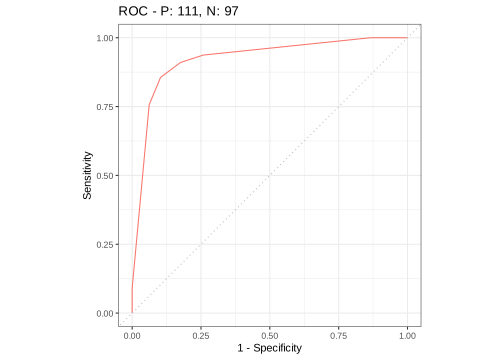
\includegraphics{03-perf-binary_files/figure-latex/binary-roc-1-1} \end{center}

We can also plot the precision-recall curve (PPV vs.~TPR).
The main difference between ROC curves and precision-recall curves (PRC) is that the number of true-negative results is not used for making a PRC.
PRCs are preferred over ROC curves for imbalanced populations.

\begin{Shaded}
\begin{Highlighting}[]
\CommentTok{\# Precision vs Recall}
\FunctionTok{autoplot}\NormalTok{(pred, }\AttributeTok{type =} \StringTok{"prc"}\NormalTok{)}
\end{Highlighting}
\end{Shaded}

\begin{center}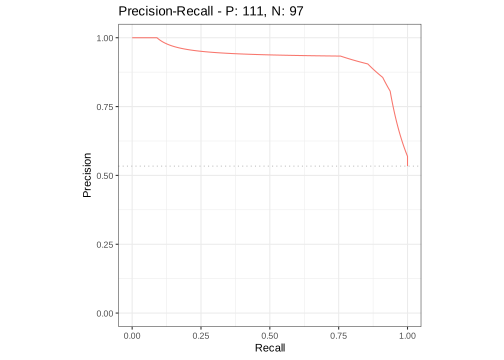
\includegraphics{03-perf-binary_files/figure-latex/binary-roc-2-1} \end{center}

\hypertarget{resampling}{%
\section{Resampling}\label{resampling}}

When evaluating the performance of a model, we are interested in its generalization performance -- how well will it perform on new data that has not been seen during training?
We can estimate the generalization performance by evaluating a model on a test set, as we have done above, that was created to contain only observations that are not contained in the training set.
There are many different strategies for partitioning a data set into training and test; in \texttt{mlr3} we call these strategies ``resampling''.
\texttt{mlr3} includes the following predefined \protect\hyperlink{resampling}{resampling} strategies:

\begin{itemize}
\tightlist
\item
  \href{https://mlr3.mlr-org.com/reference/mlr_resamplings_cv.html}{\texttt{cross\ validation}} (\texttt{"cv"}),
\item
  \href{https://mlr3.mlr-org.com/reference/mlr_resamplings_loo.html}{\texttt{leave-one-out\ cross\ validation}} (\texttt{"loo"}),
\item
  \href{https://mlr3.mlr-org.com/reference/mlr_resamplings_repeated_cv.html}{\texttt{repeated\ cross\ validation}} (\texttt{"repeated\_cv"}),
\item
  \href{https://mlr3.mlr-org.com/reference/mlr_resamplings_bootstrap.html}{\texttt{bootstrapping}} (\texttt{"bootstrap"}),
\item
  \href{https://mlr3.mlr-org.com/reference/mlr_resamplings_subsampling.html}{\texttt{subsampling}} (\texttt{"subsampling"}),
\item
  \href{https://mlr3.mlr-org.com/reference/mlr_resamplings_holdout.html}{\texttt{holdout}} (\texttt{"holdout"}),
\item
  \href{https://mlr3.mlr-org.com/reference/mlr_resamplings_insample.html}{\texttt{in-sample\ resampling}} (\texttt{"insample"}), and
\item
  \href{https://mlr3.mlr-org.com/reference/mlr_resamplings_custom.html}{\texttt{custom\ resampling}} (\texttt{"custom"}).
\end{itemize}

In particular, it is often desirable to repeatedly split the entire data in different ways to ensure that a ``lucky'' or ``unlucky'' split does not bias the generalization performance estimate.
Without resampling strategies like the ones we provide here, this is a tedious and error-prone process.

The following sections provide guidance on how to select a resampling strategy and how to use it.

Here is a graphical illustration of the resampling process in general:

\begin{center}\includegraphics{images/ml_abstraction} \end{center}

\hypertarget{resampling-settings}{%
\subsection{Settings}\label{resampling-settings}}

We will use the \href{https://mlr3.mlr-org.com/reference/mlr_tasks_penguins.html}{\texttt{penguins}} task and a simple classification tree from the \href{https://cran.r-project.org/package=rpart}{rpart} package as an example here.

\begin{Shaded}
\begin{Highlighting}[]
\FunctionTok{library}\NormalTok{(}\StringTok{"mlr3verse"}\NormalTok{)}

\NormalTok{task }\OtherTok{=} \FunctionTok{tsk}\NormalTok{(}\StringTok{"penguins"}\NormalTok{)}
\NormalTok{learner }\OtherTok{=} \FunctionTok{lrn}\NormalTok{(}\StringTok{"classif.rpart"}\NormalTok{)}
\end{Highlighting}
\end{Shaded}

When performing resampling with a dataset, we first need to define which approach should be used.
\href{https://mlr3.mlr-org.com}{mlr3} resampling strategies and their parameters can be queried by looking at the \texttt{data.table} output of the \texttt{mlr\_resamplings} dictionary; this also lists the parameters that can be changed to affect the behavior of each strategy:

\begin{Shaded}
\begin{Highlighting}[]
\FunctionTok{as.data.table}\NormalTok{(mlr\_resamplings)}
\end{Highlighting}
\end{Shaded}

\begin{verbatim}
##            key        params iters
## 1:   bootstrap ratio,repeats    30
## 2:      custom                  NA
## 3:   custom_cv                  NA
## 4:          cv         folds    10
## 5:     holdout         ratio     1
## 6:    insample                   1
## 7:         loo                  NA
## 8: repeated_cv folds,repeats   100
## 9: subsampling ratio,repeats    30
\end{verbatim}

Additional resampling methods for special use cases are available via extension packages, such as \href{https://github.com/mlr-org/mlr3spatiotemporal}{mlr3spatiotemporal} for spatial data.

What we showed in the \protect\hyperlink{train-predict}{train/predict/score} part is the equivalent of holdout resampling, done manually, so let's consider this one first.
We can retrieve elements from the dictionary \href{https://mlr3.mlr-org.com/reference/mlr_resamplings.html}{\texttt{mlr\_resamplings}} via \texttt{\$get()} or the convenience function \href{https://mlr3.mlr-org.com/reference/mlr_sugar.html}{\texttt{rsmp()}}:

\begin{Shaded}
\begin{Highlighting}[]
\NormalTok{resampling }\OtherTok{=} \FunctionTok{rsmp}\NormalTok{(}\StringTok{"holdout"}\NormalTok{)}
\FunctionTok{print}\NormalTok{(resampling)}
\end{Highlighting}
\end{Shaded}

\begin{verbatim}
## <ResamplingHoldout> with 1 iterations
## * Instantiated: FALSE
## * Parameters: ratio=0.6667
\end{verbatim}

Note that the \texttt{\$is\_instantiated} field is set to \texttt{FALSE}.
This means we did not actually apply the strategy to a dataset yet.

By default we get a .66/.33 split of the data into training and test.
There are two ways in which this ratio can be changed:

\begin{enumerate}
\def\labelenumi{\arabic{enumi}.}
\tightlist
\item
  Overwriting the slot in \texttt{\$param\_set\$values} using a named list:
\end{enumerate}

\begin{Shaded}
\begin{Highlighting}[]
\NormalTok{resampling}\SpecialCharTok{$}\NormalTok{param\_set}\SpecialCharTok{$}\NormalTok{values }\OtherTok{=} \FunctionTok{list}\NormalTok{(}\AttributeTok{ratio =} \FloatTok{0.8}\NormalTok{)}
\end{Highlighting}
\end{Shaded}

\begin{enumerate}
\def\labelenumi{\arabic{enumi}.}
\setcounter{enumi}{1}
\tightlist
\item
  Specifying the resampling parameters directly during construction:
\end{enumerate}

\begin{Shaded}
\begin{Highlighting}[]
\FunctionTok{rsmp}\NormalTok{(}\StringTok{"holdout"}\NormalTok{, }\AttributeTok{ratio =} \FloatTok{0.8}\NormalTok{)}
\end{Highlighting}
\end{Shaded}

\begin{verbatim}
## <ResamplingHoldout> with 1 iterations
## * Instantiated: FALSE
## * Parameters: ratio=0.8
\end{verbatim}

\hypertarget{resampling-inst}{%
\subsection{Instantiation}\label{resampling-inst}}

So far we have only chosen a resampling strategy; we now need to instantiate it with data.

To actually perform the splitting and obtain indices for the training and the test split, the resampling needs a \href{https://mlr3.mlr-org.com/reference/Task.html}{\texttt{Task}}.
By calling the method \texttt{instantiate()}, we split the indices of the data into indices for training and test sets.
These resulting indices are stored in the \href{https://mlr3.mlr-org.com/reference/Resampling.html}{\texttt{Resampling}} objects.

\begin{Shaded}
\begin{Highlighting}[]
\NormalTok{resampling}\SpecialCharTok{$}\FunctionTok{instantiate}\NormalTok{(task)}
\FunctionTok{str}\NormalTok{(resampling}\SpecialCharTok{$}\FunctionTok{train\_set}\NormalTok{(}\DecValTok{1}\NormalTok{))}
\end{Highlighting}
\end{Shaded}

\begin{verbatim}
##  int [1:275] 1 3 4 5 6 7 9 11 12 13 ...
\end{verbatim}

\begin{Shaded}
\begin{Highlighting}[]
\FunctionTok{str}\NormalTok{(resampling}\SpecialCharTok{$}\FunctionTok{test\_set}\NormalTok{(}\DecValTok{1}\NormalTok{))}
\end{Highlighting}
\end{Shaded}

\begin{verbatim}
##  int [1:69] 2 8 10 18 21 22 26 28 29 42 ...
\end{verbatim}

Note that if you want to compare multiple \protect\hyperlink{learners}{Learners} in a fair manner, using the same instantiated resampling for each learner is mandatory, such that each learner gets exactly the same training data and the performance of the trained model is evaluated in exactly the same test set.
A way to greatly simplify the comparison of multiple learners is discussed in the \protect\hyperlink{benchmarking}{section on benchmarking}.

\hypertarget{resampling-exec}{%
\subsection{Execution}\label{resampling-exec}}

With a \href{https://mlr3.mlr-org.com/reference/Task.html}{\texttt{Task}}, a \href{https://mlr3.mlr-org.com/reference/Learner.html}{\texttt{Learner}}, and a \href{https://mlr3.mlr-org.com/reference/Resampling.html}{\texttt{Resampling}} object we can call \href{https://mlr3.mlr-org.com/reference/resample.html}{\texttt{resample()}}, which fits the learner on the training set and evaluates it on the test set.
This may happen multiple times, depending on the given resampling strategy.
The result of running the \href{https://mlr3.mlr-org.com/reference/resample.html}{\texttt{resample()}} function is a \href{https://mlr3.mlr-org.com/reference/ResampleResult.html}{\texttt{ResampleResult}} object.
We can tell \href{https://mlr3.mlr-org.com/reference/resample.html}{\texttt{resample()}} to keep the fitted models (for example for later inspection) by setting the \texttt{store\_models} option to \texttt{TRUE}and then starting the computation:

\begin{Shaded}
\begin{Highlighting}[]
\NormalTok{task }\OtherTok{=} \FunctionTok{tsk}\NormalTok{(}\StringTok{"penguins"}\NormalTok{)}
\NormalTok{learner }\OtherTok{=} \FunctionTok{lrn}\NormalTok{(}\StringTok{"classif.rpart"}\NormalTok{, }\AttributeTok{maxdepth =} \DecValTok{3}\NormalTok{, }\AttributeTok{predict\_type =} \StringTok{"prob"}\NormalTok{)}
\NormalTok{resampling }\OtherTok{=} \FunctionTok{rsmp}\NormalTok{(}\StringTok{"cv"}\NormalTok{, }\AttributeTok{folds =} \DecValTok{3}\NormalTok{)}

\NormalTok{rr }\OtherTok{=} \FunctionTok{resample}\NormalTok{(task, learner, resampling, }\AttributeTok{store\_models =} \ConstantTok{TRUE}\NormalTok{)}
\FunctionTok{print}\NormalTok{(rr)}
\end{Highlighting}
\end{Shaded}

\begin{verbatim}
## <ResampleResult> of 3 iterations
## * Task: penguins
## * Learner: classif.rpart
## * Warnings: 0 in 0 iterations
## * Errors: 0 in 0 iterations
\end{verbatim}

Here we use a three-fold cross-validation resampling, which trains and evaluates on three different training and test sets.
The returned \href{https://mlr3.mlr-org.com/reference/ResampleResult.html}{\texttt{ResampleResult}}, stored as \texttt{rr}, provides various getters to access and aggregate the stored information.
Here are a few examples:

\begin{itemize}
\item
  Calculate the average performance across all resampling iterations, in terms of classification error:

\begin{Shaded}
\begin{Highlighting}[]
\NormalTok{rr}\SpecialCharTok{$}\FunctionTok{aggregate}\NormalTok{(}\FunctionTok{msr}\NormalTok{(}\StringTok{"classif.ce"}\NormalTok{))}
\end{Highlighting}
\end{Shaded}

\begin{verbatim}
## classif.ce 
##     0.0552
\end{verbatim}
\item
  Extract the performance for the individual resampling iterations:

\begin{Shaded}
\begin{Highlighting}[]
\NormalTok{rr}\SpecialCharTok{$}\FunctionTok{score}\NormalTok{(}\FunctionTok{msr}\NormalTok{(}\StringTok{"classif.ce"}\NormalTok{))}
\end{Highlighting}
\end{Shaded}

\begin{verbatim}
##                 task  task_id                   learner    learner_id
## 1: <TaskClassif[49]> penguins <LearnerClassifRpart[37]> classif.rpart
## 2: <TaskClassif[49]> penguins <LearnerClassifRpart[37]> classif.rpart
## 3: <TaskClassif[49]> penguins <LearnerClassifRpart[37]> classif.rpart
##            resampling resampling_id iteration              prediction
## 1: <ResamplingCV[19]>            cv         1 <PredictionClassif[20]>
## 2: <ResamplingCV[19]>            cv         2 <PredictionClassif[20]>
## 3: <ResamplingCV[19]>            cv         3 <PredictionClassif[20]>
##    classif.ce
## 1:    0.05217
## 2:    0.06957
## 3:    0.04386
\end{verbatim}

  This is useful to check if one (or more) of the iterations are very different from the average.
\item
  Check for warnings or errors:

\begin{Shaded}
\begin{Highlighting}[]
\NormalTok{rr}\SpecialCharTok{$}\NormalTok{warnings}
\end{Highlighting}
\end{Shaded}

\begin{verbatim}
## Empty data.table (0 rows and 2 cols): iteration,msg
\end{verbatim}

\begin{Shaded}
\begin{Highlighting}[]
\NormalTok{rr}\SpecialCharTok{$}\NormalTok{errors}
\end{Highlighting}
\end{Shaded}

\begin{verbatim}
## Empty data.table (0 rows and 2 cols): iteration,msg
\end{verbatim}
\item
  Extract and inspect the resampling splits; this allows to see in detail which observations were used for what purpose when:

\begin{Shaded}
\begin{Highlighting}[]
\NormalTok{rr}\SpecialCharTok{$}\NormalTok{resampling}
\end{Highlighting}
\end{Shaded}

\begin{verbatim}
## <ResamplingCV> with 3 iterations
## * Instantiated: TRUE
## * Parameters: folds=3
\end{verbatim}

\begin{Shaded}
\begin{Highlighting}[]
\NormalTok{rr}\SpecialCharTok{$}\NormalTok{resampling}\SpecialCharTok{$}\NormalTok{iters}
\end{Highlighting}
\end{Shaded}

\begin{verbatim}
## [1] 3
\end{verbatim}

\begin{Shaded}
\begin{Highlighting}[]
\FunctionTok{str}\NormalTok{(rr}\SpecialCharTok{$}\NormalTok{resampling}\SpecialCharTok{$}\FunctionTok{test\_set}\NormalTok{(}\DecValTok{1}\NormalTok{))}
\end{Highlighting}
\end{Shaded}

\begin{verbatim}
##  int [1:115] 5 6 7 12 14 16 22 23 27 29 ...
\end{verbatim}

\begin{Shaded}
\begin{Highlighting}[]
\FunctionTok{str}\NormalTok{(rr}\SpecialCharTok{$}\NormalTok{resampling}\SpecialCharTok{$}\FunctionTok{train\_set}\NormalTok{(}\DecValTok{1}\NormalTok{))}
\end{Highlighting}
\end{Shaded}

\begin{verbatim}
##  int [1:229] 1 2 3 4 8 9 11 13 15 18 ...
\end{verbatim}
\item
  Retrieve the model trained in a specific iteration and inspect it, for example to investigate why the performance in this iteration was very different from the average:

\begin{Shaded}
\begin{Highlighting}[]
\NormalTok{lrn }\OtherTok{=}\NormalTok{ rr}\SpecialCharTok{$}\NormalTok{learners[[}\DecValTok{1}\NormalTok{]]}
\NormalTok{lrn}\SpecialCharTok{$}\NormalTok{model}
\end{Highlighting}
\end{Shaded}

\begin{verbatim}
## n= 229 
## 
## node), split, n, loss, yval, (yprob)
##       * denotes terminal node
## 
## 1) root 229 127 Adelie (0.445415 0.179039 0.375546)  
##   2) flipper_length< 206.5 139  39 Adelie (0.719424 0.273381 0.007194)  
##     4) bill_length< 44.2 101   3 Adelie (0.970297 0.029703 0.000000) *
##     5) bill_length>=44.2 38   3 Chinstrap (0.052632 0.921053 0.026316) *
##   3) flipper_length>=206.5 90   5 Gentoo (0.022222 0.033333 0.944444) *
\end{verbatim}
\item
  Extract the individual predictions:

\begin{Shaded}
\begin{Highlighting}[]
\NormalTok{rr}\SpecialCharTok{$}\FunctionTok{prediction}\NormalTok{() }\CommentTok{\# all predictions merged into a single Prediction object}
\end{Highlighting}
\end{Shaded}

\begin{verbatim}
## <PredictionClassif> for 344 observations:
##     row_ids     truth  response prob.Adelie prob.Chinstrap prob.Gentoo
##           5    Adelie    Adelie     0.97030        0.02970     0.00000
##           6    Adelie    Adelie     0.97030        0.02970     0.00000
##           7    Adelie    Adelie     0.97030        0.02970     0.00000
## ---                                                                   
##         340 Chinstrap    Gentoo     0.01299        0.02597     0.96104
##         343 Chinstrap    Gentoo     0.01299        0.02597     0.96104
##         344 Chinstrap Chinstrap     0.09756        0.87805     0.02439
\end{verbatim}

\begin{Shaded}
\begin{Highlighting}[]
\NormalTok{rr}\SpecialCharTok{$}\FunctionTok{predictions}\NormalTok{()[[}\DecValTok{1}\NormalTok{]] }\CommentTok{\# predictions of first resampling iteration}
\end{Highlighting}
\end{Shaded}

\begin{verbatim}
## <PredictionClassif> for 115 observations:
##     row_ids     truth  response prob.Adelie prob.Chinstrap prob.Gentoo
##           5    Adelie    Adelie     0.97030         0.0297     0.00000
##           6    Adelie    Adelie     0.97030         0.0297     0.00000
##           7    Adelie    Adelie     0.97030         0.0297     0.00000
## ---                                                                   
##         338 Chinstrap Chinstrap     0.05263         0.9211     0.02632
##         341 Chinstrap    Adelie     0.97030         0.0297     0.00000
##         342 Chinstrap Chinstrap     0.05263         0.9211     0.02632
\end{verbatim}
\item
  Filter the result to only keep specified resampling iterations:

\begin{Shaded}
\begin{Highlighting}[]
\NormalTok{rr}\SpecialCharTok{$}\FunctionTok{filter}\NormalTok{(}\FunctionTok{c}\NormalTok{(}\DecValTok{1}\NormalTok{, }\DecValTok{3}\NormalTok{))}
\FunctionTok{print}\NormalTok{(rr)}
\end{Highlighting}
\end{Shaded}

\begin{verbatim}
## <ResampleResult> of 2 iterations
## * Task: penguins
## * Learner: classif.rpart
## * Warnings: 0 in 0 iterations
## * Errors: 0 in 0 iterations
\end{verbatim}
\end{itemize}

\hypertarget{resamp-custom}{%
\subsection{Custom resampling}\label{resamp-custom}}

Sometimes it is necessary to perform resampling with custom splits, e.g.~to reproduce results reported in a study.
A manual resampling instance can be created using the \texttt{"custom"} template.

\begin{Shaded}
\begin{Highlighting}[]
\NormalTok{resampling }\OtherTok{=} \FunctionTok{rsmp}\NormalTok{(}\StringTok{"custom"}\NormalTok{)}
\NormalTok{resampling}\SpecialCharTok{$}\FunctionTok{instantiate}\NormalTok{(task,}
  \AttributeTok{train =} \FunctionTok{list}\NormalTok{(}\FunctionTok{c}\NormalTok{(}\DecValTok{1}\SpecialCharTok{:}\DecValTok{10}\NormalTok{, }\DecValTok{51}\SpecialCharTok{:}\DecValTok{60}\NormalTok{, }\DecValTok{101}\SpecialCharTok{:}\DecValTok{110}\NormalTok{)),}
  \AttributeTok{test =} \FunctionTok{list}\NormalTok{(}\FunctionTok{c}\NormalTok{(}\DecValTok{11}\SpecialCharTok{:}\DecValTok{20}\NormalTok{, }\DecValTok{61}\SpecialCharTok{:}\DecValTok{70}\NormalTok{, }\DecValTok{111}\SpecialCharTok{:}\DecValTok{120}\NormalTok{))}
\NormalTok{)}
\NormalTok{resampling}\SpecialCharTok{$}\NormalTok{iters}
\end{Highlighting}
\end{Shaded}

\begin{verbatim}
## [1] 1
\end{verbatim}

\begin{Shaded}
\begin{Highlighting}[]
\NormalTok{resampling}\SpecialCharTok{$}\FunctionTok{train\_set}\NormalTok{(}\DecValTok{1}\NormalTok{)}
\end{Highlighting}
\end{Shaded}

\begin{verbatim}
##  [1]   1   2   3   4   5   6   7   8   9  10  51  52  53  54  55  56  57  58  59
## [20]  60 101 102 103 104 105 106 107 108 109 110
\end{verbatim}

\begin{Shaded}
\begin{Highlighting}[]
\NormalTok{resampling}\SpecialCharTok{$}\FunctionTok{test\_set}\NormalTok{(}\DecValTok{1}\NormalTok{)}
\end{Highlighting}
\end{Shaded}

\begin{verbatim}
##  [1]  11  12  13  14  15  16  17  18  19  20  61  62  63  64  65  66  67  68  69
## [20]  70 111 112 113 114 115 116 117 118 119 120
\end{verbatim}

\hypertarget{resampling-with-predefined-groups}{%
\subsection{Resampling with (predefined) groups}\label{resampling-with-predefined-groups}}

In some cases, it is desirable to keep observations together, i.e.~to not separate them into training and test set.
This can be defined through the column role \texttt{"group"} during Task creation, i.e.~a special column in the data specifies the groups (see also the \href{https://mlr3.mlr-org.com/reference/Resampling.html\#grouping-blocking}{help page} on this column role).
In \texttt{mlr} this was called ``blocking''.
See also the mlr3gallery post on \href{https://mlr3gallery.mlr-org.com/posts/2020-03-30-stratification-blocking/}{this topic} for a practical example.

\hypertarget{autoplot-resampleresult}{%
\subsection{Plotting Resample Results}\label{autoplot-resampleresult}}

\href{https://mlr3viz.mlr-org.com}{mlr3viz} provides a \href{https://www.rdocumentation.org/packages/ggplot2/topics/autoplot}{\texttt{autoplot()}} method for resampling results.
As an example, we create a binary classification task with two features, perform a resampling with a 10-fold cross-validation and visualize the results:

\begin{Shaded}
\begin{Highlighting}[]
\NormalTok{task }\OtherTok{=} \FunctionTok{tsk}\NormalTok{(}\StringTok{"pima"}\NormalTok{)}
\NormalTok{task}\SpecialCharTok{$}\FunctionTok{select}\NormalTok{(}\FunctionTok{c}\NormalTok{(}\StringTok{"glucose"}\NormalTok{, }\StringTok{"mass"}\NormalTok{))}
\NormalTok{learner }\OtherTok{=} \FunctionTok{lrn}\NormalTok{(}\StringTok{"classif.rpart"}\NormalTok{, }\AttributeTok{predict\_type =} \StringTok{"prob"}\NormalTok{)}
\NormalTok{rr }\OtherTok{=} \FunctionTok{resample}\NormalTok{(task, learner, }\FunctionTok{rsmp}\NormalTok{(}\StringTok{"cv"}\NormalTok{), }\AttributeTok{store\_models =} \ConstantTok{TRUE}\NormalTok{)}

\CommentTok{\# boxplot of AUC values across the 10 folds}
\FunctionTok{autoplot}\NormalTok{(rr, }\AttributeTok{measure =} \FunctionTok{msr}\NormalTok{(}\StringTok{"classif.auc"}\NormalTok{))}
\end{Highlighting}
\end{Shaded}

\begin{center}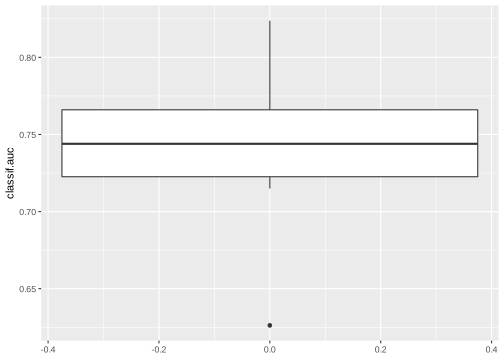
\includegraphics{03-perf-resampling_files/figure-latex/02-basics-resampling-017-1} \end{center}

\begin{Shaded}
\begin{Highlighting}[]
\CommentTok{\# ROC curve, averaged over 10 folds}
\FunctionTok{autoplot}\NormalTok{(rr, }\AttributeTok{type =} \StringTok{"roc"}\NormalTok{)}
\end{Highlighting}
\end{Shaded}

\begin{center}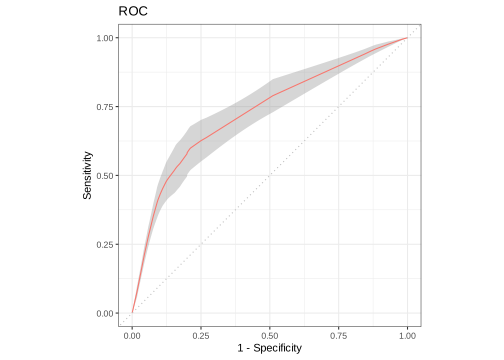
\includegraphics{03-perf-resampling_files/figure-latex/02-basics-resampling-017-2} \end{center}

We can also plot the predictions of individual models:

\begin{Shaded}
\begin{Highlighting}[]
\CommentTok{\# learner predictions for the first fold}
\NormalTok{rr}\SpecialCharTok{$}\FunctionTok{filter}\NormalTok{(}\DecValTok{1}\NormalTok{)}
\FunctionTok{autoplot}\NormalTok{(rr, }\AttributeTok{type =} \StringTok{"prediction"}\NormalTok{)}
\end{Highlighting}
\end{Shaded}

\begin{verbatim}
## Warning: Removed 1 rows containing missing values (geom_point).
\end{verbatim}

\begin{center}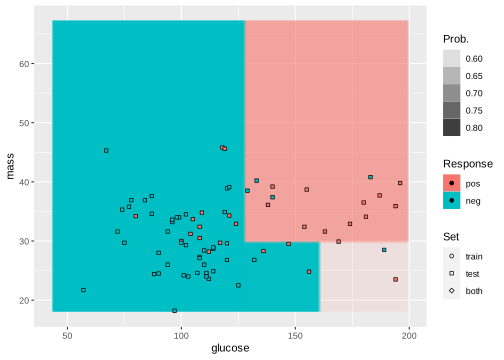
\includegraphics{03-perf-resampling_files/figure-latex/02-basics-resampling-017-1-1} \end{center}

All available plot types are listed on the manual page of \href{https://mlr3viz.mlr-org.com/reference/autoplot.ResampleResult.html}{\texttt{autoplot.ResampleResult()}}.

\hypertarget{benchmarking}{%
\section{Benchmarking}\label{benchmarking}}

Comparing the performance of different learners on multiple tasks and/or different resampling schemes is a common task.
This operation is usually referred to as ``benchmarking'' in the field of machine learning.
The \href{https://mlr3.mlr-org.com}{mlr3} package offers the \href{https://mlr3.mlr-org.com/reference/benchmark.html}{\texttt{benchmark()}} convenience function that takes care of most of the work of repeatedly training and evaluating models under the same conditions.

\hypertarget{bm-design}{%
\subsection{Design Creation}\label{bm-design}}

Benchmark experiments in \texttt{mlr3} are specified through a design.
Such a design is essentially a table of scenarios to be evaluated; in particular unique combinations of \href{https://mlr3.mlr-org.com/reference/Task.html}{\texttt{Task}}, \href{https://mlr3.mlr-org.com/reference/Learner.html}{\texttt{Learner}} and \href{https://mlr3.mlr-org.com/reference/Resampling.html}{\texttt{Resampling}} triplets.

We use the \href{https://mlr3.mlr-org.com/reference/benchmark_grid.html}{\texttt{benchmark\_grid()}} function to create an exhaustive design (that evaluates each learner on each task with each resampling) and instantiate the resampling properly, so that all learners are executed on the same train/test split for each tasks.
We set the learners to predict probabilities and also tell them to predict for the observations of the training set (by setting \texttt{predict\_sets} to \texttt{c("train",\ "test")}).
Additionally, we use \href{https://mlr3.mlr-org.com/reference/mlr_sugar.html}{\texttt{tsks()}}, \href{https://mlr3.mlr-org.com/reference/mlr_sugar.html}{\texttt{lrns()}}, and \href{https://mlr3.mlr-org.com/reference/mlr_sugar.html}{\texttt{rsmps()}} to retrieve lists of \href{https://mlr3.mlr-org.com/reference/Task.html}{\texttt{Task}}, \href{https://mlr3.mlr-org.com/reference/Learner.html}{\texttt{Learner}} and \href{https://mlr3.mlr-org.com/reference/Resampling.html}{\texttt{Resampling}} in the same fashion as \href{https://mlr3.mlr-org.com/reference/mlr_sugar.html}{\texttt{tsk()}}, \href{https://mlr3.mlr-org.com/reference/mlr_sugar.html}{\texttt{lrn()}} and \href{https://mlr3.mlr-org.com/reference/mlr_sugar.html}{\texttt{rsmp()}}.

\begin{Shaded}
\begin{Highlighting}[]
\FunctionTok{library}\NormalTok{(}\StringTok{"mlr3verse"}\NormalTok{)}

\NormalTok{design }\OtherTok{=} \FunctionTok{benchmark\_grid}\NormalTok{(}
  \AttributeTok{tasks =} \FunctionTok{tsks}\NormalTok{(}\FunctionTok{c}\NormalTok{(}\StringTok{"spam"}\NormalTok{, }\StringTok{"german\_credit"}\NormalTok{, }\StringTok{"sonar"}\NormalTok{)),}
  \AttributeTok{learners =} \FunctionTok{lrns}\NormalTok{(}\FunctionTok{c}\NormalTok{(}\StringTok{"classif.ranger"}\NormalTok{, }\StringTok{"classif.rpart"}\NormalTok{, }\StringTok{"classif.featureless"}\NormalTok{),}
    \AttributeTok{predict\_type =} \StringTok{"prob"}\NormalTok{, }\AttributeTok{predict\_sets =} \FunctionTok{c}\NormalTok{(}\StringTok{"train"}\NormalTok{, }\StringTok{"test"}\NormalTok{)),}
  \AttributeTok{resamplings =} \FunctionTok{rsmps}\NormalTok{(}\StringTok{"cv"}\NormalTok{, }\AttributeTok{folds =} \DecValTok{3}\NormalTok{)}
\NormalTok{)}
\FunctionTok{print}\NormalTok{(design)}
\end{Highlighting}
\end{Shaded}

\begin{verbatim}
##                 task                         learner         resampling
## 1: <TaskClassif[49]>      <LearnerClassifRanger[37]> <ResamplingCV[19]>
## 2: <TaskClassif[49]>       <LearnerClassifRpart[37]> <ResamplingCV[19]>
## 3: <TaskClassif[49]> <LearnerClassifFeatureless[37]> <ResamplingCV[19]>
## 4: <TaskClassif[49]>      <LearnerClassifRanger[37]> <ResamplingCV[19]>
## 5: <TaskClassif[49]>       <LearnerClassifRpart[37]> <ResamplingCV[19]>
## 6: <TaskClassif[49]> <LearnerClassifFeatureless[37]> <ResamplingCV[19]>
## 7: <TaskClassif[49]>      <LearnerClassifRanger[37]> <ResamplingCV[19]>
## 8: <TaskClassif[49]>       <LearnerClassifRpart[37]> <ResamplingCV[19]>
## 9: <TaskClassif[49]> <LearnerClassifFeatureless[37]> <ResamplingCV[19]>
\end{verbatim}

The created \texttt{design} can be passed to \href{https://mlr3.mlr-org.com/reference/benchmark.html}{\texttt{benchmark()}} to start the computation.
It is also possible to create a custom design manually, for example to exclude certain task-learner combinations.
However, if you create a custom task with \texttt{data.table()}, the train/test splits will be different for each row of the design if you do not \protect\hyperlink{resampling-inst}{\textbf{manually instantiate}} the resampling before creating the design.
See the help page on \href{https://mlr3.mlr-org.com/reference/benchmark_grid.html}{\texttt{benchmark\_grid()}} for an example.

\hypertarget{bm-exec}{%
\subsection{Execution and Aggregation of Results}\label{bm-exec}}

After the \protect\hyperlink{bm-design}{benchmark design} is ready, we can call \href{https://mlr3.mlr-org.com/reference/benchmark.html}{\texttt{benchmark()}} on it:

\begin{Shaded}
\begin{Highlighting}[]
\NormalTok{bmr }\OtherTok{=} \FunctionTok{benchmark}\NormalTok{(design)}
\end{Highlighting}
\end{Shaded}

Note that we did not have to instantiate the resampling manually.
\href{https://mlr3.mlr-org.com/reference/benchmark_grid.html}{\texttt{benchmark\_grid()}} took care of it for us: each resampling strategy is instantiated once for each task during the construction of the exhaustive grid.

Once the benchmarking is done (and, depending on the size of your design, this can take quite some time), we can aggregate the performance with \texttt{\$aggregate()}.
We create two measures to calculate the area under the curve (AUC) for the training and the test set:

\begin{Shaded}
\begin{Highlighting}[]
\NormalTok{measures }\OtherTok{=} \FunctionTok{list}\NormalTok{(}
  \FunctionTok{msr}\NormalTok{(}\StringTok{"classif.auc"}\NormalTok{, }\AttributeTok{predict\_sets =} \StringTok{"train"}\NormalTok{, }\AttributeTok{id =} \StringTok{"auc\_train"}\NormalTok{),}
  \FunctionTok{msr}\NormalTok{(}\StringTok{"classif.auc"}\NormalTok{, }\AttributeTok{id =} \StringTok{"auc\_test"}\NormalTok{)}
\NormalTok{)}

\NormalTok{tab }\OtherTok{=}\NormalTok{ bmr}\SpecialCharTok{$}\FunctionTok{aggregate}\NormalTok{(measures)}
\FunctionTok{print}\NormalTok{(tab)}
\end{Highlighting}
\end{Shaded}

\begin{verbatim}
##    nr      resample_result       task_id          learner_id resampling_id
## 1:  1 <ResampleResult[22]>          spam      classif.ranger            cv
## 2:  2 <ResampleResult[22]>          spam       classif.rpart            cv
## 3:  3 <ResampleResult[22]>          spam classif.featureless            cv
## 4:  4 <ResampleResult[22]> german_credit      classif.ranger            cv
## 5:  5 <ResampleResult[22]> german_credit       classif.rpart            cv
## 6:  6 <ResampleResult[22]> german_credit classif.featureless            cv
## 7:  7 <ResampleResult[22]>         sonar      classif.ranger            cv
## 8:  8 <ResampleResult[22]>         sonar       classif.rpart            cv
## 9:  9 <ResampleResult[22]>         sonar classif.featureless            cv
##    iters auc_train auc_test
## 1:     3    0.9995   0.9847
## 2:     3    0.9124   0.8957
## 3:     3    0.5000   0.5000
## 4:     3    0.9987   0.7919
## 5:     3    0.8172   0.7075
## 6:     3    0.5000   0.5000
## 7:     3    1.0000   0.9063
## 8:     3    0.8759   0.6972
## 9:     3    0.5000   0.5000
\end{verbatim}

We can aggregate the results even further.
For example, we might be interested to know which learner performed best across all tasks.
Simply aggregating the performances with the mean is usually not statistically sound.
Instead, we calculate the rank statistic for each learner, grouped by task.
Then the calculated ranks, grouped by learner, are aggregated with the \href{https://cran.r-project.org/package=data.table}{data.table} package.
As larger AUC scores are better, we multiply the values by \(-1\) such that the best learner has a rank of \(1\).

\begin{Shaded}
\begin{Highlighting}[]
\FunctionTok{library}\NormalTok{(}\StringTok{"data.table"}\NormalTok{)}
\CommentTok{\# group by levels of task\_id, return columns:}
\CommentTok{\# {-} learner\_id}
\CommentTok{\# {-} rank of col \textquotesingle{}{-}auc\_train\textquotesingle{} (per level of learner\_id)}
\CommentTok{\# {-} rank of col \textquotesingle{}{-}auc\_test\textquotesingle{} (per level of learner\_id)}
\NormalTok{ranks }\OtherTok{=}\NormalTok{ tab[, .(learner\_id, }\AttributeTok{rank\_train =} \FunctionTok{rank}\NormalTok{(}\SpecialCharTok{{-}}\NormalTok{auc\_train), }\AttributeTok{rank\_test =} \FunctionTok{rank}\NormalTok{(}\SpecialCharTok{{-}}\NormalTok{auc\_test)), by }\OtherTok{=}\NormalTok{ task\_id]}
\FunctionTok{print}\NormalTok{(ranks)}
\end{Highlighting}
\end{Shaded}

\begin{verbatim}
##          task_id          learner_id rank_train rank_test
## 1:          spam      classif.ranger          1         1
## 2:          spam       classif.rpart          2         2
## 3:          spam classif.featureless          3         3
## 4: german_credit      classif.ranger          1         1
## 5: german_credit       classif.rpart          2         2
## 6: german_credit classif.featureless          3         3
## 7:         sonar      classif.ranger          1         1
## 8:         sonar       classif.rpart          2         2
## 9:         sonar classif.featureless          3         3
\end{verbatim}

\begin{Shaded}
\begin{Highlighting}[]
\CommentTok{\# group by levels of learner\_id, return columns:}
\CommentTok{\# {-} mean rank of col \textquotesingle{}rank\_train\textquotesingle{} (per level of learner\_id)}
\CommentTok{\# {-} mean rank of col \textquotesingle{}rank\_test\textquotesingle{} (per level of learner\_id)}
\NormalTok{ranks }\OtherTok{=}\NormalTok{ ranks[, .(}\AttributeTok{mrank\_train =} \FunctionTok{mean}\NormalTok{(rank\_train), }\AttributeTok{mrank\_test =} \FunctionTok{mean}\NormalTok{(rank\_test)), by }\OtherTok{=}\NormalTok{ learner\_id]}

\CommentTok{\# print the final table, ordered by mean rank of AUC test}
\NormalTok{ranks[}\FunctionTok{order}\NormalTok{(mrank\_test)]}
\end{Highlighting}
\end{Shaded}

\begin{verbatim}
##             learner_id mrank_train mrank_test
## 1:      classif.ranger           1          1
## 2:       classif.rpart           2          2
## 3: classif.featureless           3          3
\end{verbatim}

Unsurprisingly, the featureless learner is worse overall.
The winner is the classification forest, which outperforms a single classification tree.

\hypertarget{autoplot-benchmarkresult}{%
\subsection{Plotting Benchmark Results}\label{autoplot-benchmarkresult}}

Similar to \protect\hyperlink{autoplot-task}{tasks}, \protect\hyperlink{autoplot-prediction}{predictions}, or \protect\hyperlink{autoplot-resampleresult}{resample results}, \href{https://mlr3viz.mlr-org.com}{mlr3viz} also provides a \href{https://www.rdocumentation.org/packages/ggplot2/topics/autoplot}{\texttt{autoplot()}} method for benchmark results.

\begin{Shaded}
\begin{Highlighting}[]
\FunctionTok{autoplot}\NormalTok{(bmr) }\SpecialCharTok{+}\NormalTok{ ggplot2}\SpecialCharTok{::}\FunctionTok{theme}\NormalTok{(}\AttributeTok{axis.text.x =}\NormalTok{ ggplot2}\SpecialCharTok{::}\FunctionTok{element\_text}\NormalTok{(}\AttributeTok{angle =} \DecValTok{45}\NormalTok{, }\AttributeTok{hjust =} \DecValTok{1}\NormalTok{))}
\end{Highlighting}
\end{Shaded}

\begin{center}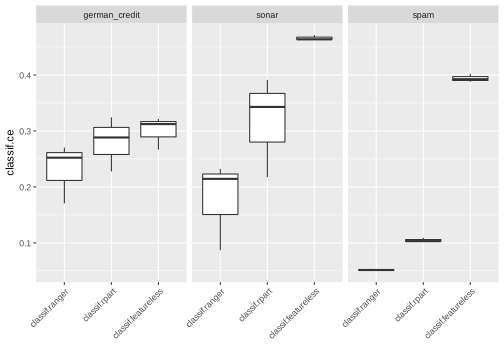
\includegraphics{03-perf-benchmarking_files/figure-latex/02-basics-benchmarking-005-1} \end{center}

Such a plot gives a nice overview of the overall performance and how learners compare on different tasks in an intuitive way.

We can also plot ROC (receiver operating characteristics) curves.
We filter the \href{https://mlr3.mlr-org.com/reference/BenchmarkResult.html}{\texttt{BenchmarkResult}} to only contain a single \href{https://mlr3.mlr-org.com/reference/Task.html}{\texttt{Task}}, then we simply plot the result:

\begin{Shaded}
\begin{Highlighting}[]
\NormalTok{bmr\_small }\OtherTok{=}\NormalTok{ bmr}\SpecialCharTok{$}\FunctionTok{clone}\NormalTok{()}\SpecialCharTok{$}\FunctionTok{filter}\NormalTok{(}\AttributeTok{task\_id =} \StringTok{"german\_credit"}\NormalTok{)}
\FunctionTok{autoplot}\NormalTok{(bmr\_small, }\AttributeTok{type =} \StringTok{"roc"}\NormalTok{)}
\end{Highlighting}
\end{Shaded}

\begin{center}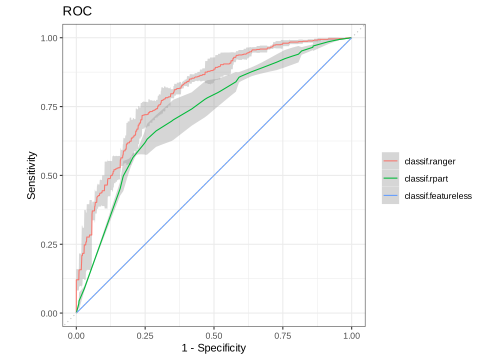
\includegraphics{03-perf-benchmarking_files/figure-latex/02-basics-benchmarking-006-1} \end{center}

All available plot types are listed on the manual page of \href{https://mlr3viz.mlr-org.com/reference/autoplot.BenchmarkResult.html}{\texttt{autoplot.BenchmarkResult()}}.

\hypertarget{bm-resamp}{%
\subsection{Extracting ResampleResults}\label{bm-resamp}}

A \href{https://mlr3.mlr-org.com/reference/BenchmarkResult.html}{\texttt{BenchmarkResult}} object is essentially a collection of multiple \href{https://mlr3.mlr-org.com/reference/ResampleResult.html}{\texttt{ResampleResult}} objects.
As these are stored in a column of the aggregated \texttt{data.table()}, we can easily extract them:

\begin{Shaded}
\begin{Highlighting}[]
\NormalTok{tab }\OtherTok{=}\NormalTok{ bmr}\SpecialCharTok{$}\FunctionTok{aggregate}\NormalTok{(measures)}
\NormalTok{rr }\OtherTok{=}\NormalTok{ tab[task\_id }\SpecialCharTok{==} \StringTok{"german\_credit"} \SpecialCharTok{\&}\NormalTok{ learner\_id }\SpecialCharTok{==} \StringTok{"classif.ranger"}\NormalTok{]}\SpecialCharTok{$}\NormalTok{resample\_result[[}\DecValTok{1}\NormalTok{]]}
\FunctionTok{print}\NormalTok{(rr)}
\end{Highlighting}
\end{Shaded}

\begin{verbatim}
## <ResampleResult> of 3 iterations
## * Task: german_credit
## * Learner: classif.ranger
## * Warnings: 0 in 0 iterations
## * Errors: 0 in 0 iterations
\end{verbatim}

We can now investigate this resampling and even single resampling iterations using one of the approaches shown in \protect\hyperlink{resampling}{the previous section}:

\begin{Shaded}
\begin{Highlighting}[]
\NormalTok{measure }\OtherTok{=} \FunctionTok{msr}\NormalTok{(}\StringTok{"classif.auc"}\NormalTok{)}
\NormalTok{rr}\SpecialCharTok{$}\FunctionTok{aggregate}\NormalTok{(measure)}
\end{Highlighting}
\end{Shaded}

\begin{verbatim}
## classif.auc 
##      0.7919
\end{verbatim}

\begin{Shaded}
\begin{Highlighting}[]
\CommentTok{\# get the iteration with worst AUC}
\NormalTok{perf }\OtherTok{=}\NormalTok{ rr}\SpecialCharTok{$}\FunctionTok{score}\NormalTok{(measure)}
\NormalTok{i }\OtherTok{=} \FunctionTok{which.min}\NormalTok{(perf}\SpecialCharTok{$}\NormalTok{classif.auc)}

\CommentTok{\# get the corresponding learner and training set}
\FunctionTok{print}\NormalTok{(rr}\SpecialCharTok{$}\NormalTok{learners[[i]])}
\end{Highlighting}
\end{Shaded}

\begin{verbatim}
## <LearnerClassifRanger:classif.ranger>
## * Model: -
## * Parameters: num.threads=1
## * Packages: mlr3, mlr3learners, ranger
## * Predict Type: prob
## * Feature types: logical, integer, numeric, character, factor, ordered
## * Properties: hotstart_backward, importance, multiclass, oob_error,
##   twoclass, weights
\end{verbatim}

\begin{Shaded}
\begin{Highlighting}[]
\FunctionTok{head}\NormalTok{(rr}\SpecialCharTok{$}\NormalTok{resampling}\SpecialCharTok{$}\FunctionTok{train\_set}\NormalTok{(i))}
\end{Highlighting}
\end{Shaded}

\begin{verbatim}
## [1]  3  4  7 10 12 13
\end{verbatim}

\hypertarget{converting-and-merging}{%
\subsection{Converting and Merging}\label{converting-and-merging}}

A \href{https://mlr3.mlr-org.com/reference/ResampleResult.html}{\texttt{ResampleResult}} can be converted to a \href{https://mlr3.mlr-org.com/reference/BenchmarkResult.html}{\texttt{BenchmarkResult}} with the function \href{https://mlr3.mlr-org.com/reference/as_benchmark_result.html}{\texttt{as\_benchmark\_result()}}.
We can also merge two \href{https://mlr3.mlr-org.com/reference/BenchmarkResult.html}{\texttt{BenchmarkResults}} into a larger result object, for example for two related benchmarks that were done on different machines.

\begin{Shaded}
\begin{Highlighting}[]
\NormalTok{task }\OtherTok{=} \FunctionTok{tsk}\NormalTok{(}\StringTok{"iris"}\NormalTok{)}
\NormalTok{resampling }\OtherTok{=} \FunctionTok{rsmp}\NormalTok{(}\StringTok{"holdout"}\NormalTok{)}\SpecialCharTok{$}\FunctionTok{instantiate}\NormalTok{(task)}

\NormalTok{rr1 }\OtherTok{=} \FunctionTok{resample}\NormalTok{(task, }\FunctionTok{lrn}\NormalTok{(}\StringTok{"classif.rpart"}\NormalTok{), resampling)}
\NormalTok{rr2 }\OtherTok{=} \FunctionTok{resample}\NormalTok{(task, }\FunctionTok{lrn}\NormalTok{(}\StringTok{"classif.featureless"}\NormalTok{), resampling)}

\CommentTok{\# Cast both ResampleResults to BenchmarkResults}
\NormalTok{bmr1 }\OtherTok{=} \FunctionTok{as\_benchmark\_result}\NormalTok{(rr1)}
\NormalTok{bmr2 }\OtherTok{=} \FunctionTok{as\_benchmark\_result}\NormalTok{(rr2)}

\CommentTok{\# Merge 2nd BMR into the first BMR}
\NormalTok{bmr1}\SpecialCharTok{$}\FunctionTok{combine}\NormalTok{(bmr2)}

\NormalTok{bmr1}
\end{Highlighting}
\end{Shaded}

\begin{verbatim}
## <BenchmarkResult> of 2 rows with 2 resampling runs
##  nr task_id          learner_id resampling_id iters warnings errors
##   1    iris       classif.rpart       holdout     1        0      0
##   2    iris classif.featureless       holdout     1        0      0
\end{verbatim}

\hypertarget{optimization}{%
\chapter{Model Optimization}\label{optimization}}

In machine learning, when you are dissatisfied with the performance of a model, you might ask yourself how to best improve the model:
* Can it be improved by tweaking the hyperparameters of the learner, i.e.~the configuration options that affect its behavior?
* Or, should you just use a completely different learner for this particular task?
This chapter might help answer this question.

\textbf{Model Tuning}

Machine learning algorithms have default values set for their hyperparameters.
In many cases, these hyperparameters need to be changed by the user to achieve optimal performance on the given dataset.
While you can certainly search for hyperparameter settings that improve performance manually, we do not recommend this approach as it is tedious and rarely leads to the best performance.
Fortunately, the \texttt{mlr3} ecosystem provides packages and tools for automated tuning.
In order to tune a machine learning algorithm, you have to specify (1) the \protect\hyperlink{tuning-optimization}{search space}, (2) the \protect\hyperlink{tuning-algorithms}{optimization algorithm} (i.e.~tuning method), (3) an evaluation method (i.e.~a resampling strategy), and (4) a performance measure.

In the \protect\hyperlink{tuning}{tuning} part, we will have a look at:

\begin{itemize}
\tightlist
\item
  empirically sound \protect\hyperlink{tuning}{hyperparameter tuning},
\item
  selecting the \protect\hyperlink{tuning-optimization}{optimizing algorithm},
\item
  defining \protect\hyperlink{searchspace}{search spaces concisely},
\item
  \protect\hyperlink{tuning-triggering}{triggering} the tuning, and
\item
  \protect\hyperlink{autotuner}{automating} tuning.
\end{itemize}

We will use the \href{https://mlr3tuning.mlr-org.com}{mlr3tuning} package, which supports common tuning operations.

\textbf{Feature Selection}

Tuning the hyperparameters is only one way of improving the performance of your model.
The second part of this chapter explains \protect\hyperlink{fs}{feature selection}, also known as variable or descriptor selection.
\protect\hyperlink{fs}{Feature selection} is the process of finding the feature subset that is most relevant with respect to the prediction or for which the learner fits a model with the highest performance.
Apart from improving model performance, there are additional reasons to perform feature selection:

\begin{itemize}
\tightlist
\item
  enhance the interpretability of the model,
\item
  speed up model fitting, or
\item
  eliminate the need to collect lots of expensive features.
\end{itemize}

Here, we mostly focus on feature selection as a means for improving model performance.

There are different approaches to identify the relevant features.
In the \protect\hyperlink{fs}{feature selection} part, we describe three methods:

\begin{itemize}
\tightlist
\item
  \protect\hyperlink{fs-filter}{Filter} algorithms select features independently of the learner by scoring the different features.
\item
  \protect\hyperlink{fs-var-imp-filters}{Variable importance filters} select features that are important according the model induced by a learner.
\item
  \protect\hyperlink{fs-wrapper}{Wrapper methods} iteratively select features to optimize a performance measure, each time fitting and evaluating a model with a different subset of features.
\end{itemize}

Note that filters operate independently of learners.
Variable importance filters rely on the learner to extract information on feature importance from a trained model, for example by inspecting a learned decision tree and returning the features that are used in the first few levels.
The obtained importance values can be used to subset the data, which can then be used to train a learner.
Wrapper methods can be used with any learner but need to train the learner potentially many times, making this the most expensive method.

\textbf{Nested Resampling}

For hyperparameter tuning, a normal resampling (e.g.~a cross-validation) is no longer sufficient to ensure an unbiased evaluation.
Consider the following thought experiment to gain intuition for why this is the case.
Suppose a learner has a hyperparameter that has no real effect on the fitted model, but only introduces random noise into the predictions.
Evaluating different values for this hyperparameter, one will show the best performance (purely randomly).
This is the hyperparameter value that will be chosen as the best, although the hyperparameter has no real effect.
To discover this, another separate validation set is required -- it will reveal that the ``optimized'' setting really does not perform better than anything else.

We need a nested resampling to ensure unbiased estimates of the generalization error during hyperparameter optimization.
We discuss the following aspects in this part:

\begin{itemize}
\tightlist
\item
  \protect\hyperlink{nested-resampling}{Inner and outer resampling strategies} in nested resampling.
\item
  The \protect\hyperlink{nested-resamp-exec}{execution} of nested resampling.
\item
  The \protect\hyperlink{nested-resamp-eval}{evaluation} of resampling iterations.
\end{itemize}

\hypertarget{tuning}{%
\section{Hyperparameter Tuning}\label{tuning}}

Hyperparameters are the parameters of the learners that control how a model is fit to the data.
They are sometimes called second-level or second-order parameters of machine learning -- the parameters of the \emph{models} are the first-order parameters and ``fit'' to the data during model training.
The hyerparameters of a learner can have a major impact on the performance of a learned model, but are often only optimized in an ad-hoc manner or not at all.
This process is often called model `tuning'.

Hyperparameter tuning is supported via the \href{https://mlr3tuning.mlr-org.com}{mlr3tuning} extension package.
Below you can find an illustration of the general process:

\begin{center}\includegraphics{images/tuning_process} \end{center}

At the heart of \href{https://mlr3tuning.mlr-org.com}{mlr3tuning} are the R6 classes

\begin{itemize}
\tightlist
\item
  \href{https://mlr3tuning.mlr-org.com/reference/TuningInstanceSingleCrit.html}{\texttt{TuningInstanceSingleCrit}}, \href{https://mlr3tuning.mlr-org.com/reference/TuningInstanceMultiCrit.html}{\texttt{TuningInstanceMultiCrit}} to describe the tuning problem and store the results, and
\item
  \href{https://mlr3tuning.mlr-org.com/reference/Tuner.html}{\texttt{Tuner}} as the base class for implementations of tuning algorithms.
\end{itemize}

\hypertarget{tuning-optimization}{%
\subsection{\texorpdfstring{The \texttt{TuningInstance*} Classes}{The TuningInstance* Classes}}\label{tuning-optimization}}

We will examine the optimization of a simple classification tree on the \href{https://mlr3.mlr-org.com/reference/mlr_tasks_pima.html}{\texttt{Pima\ Indian\ Diabetes}} data set as an introductory example here.

\begin{Shaded}
\begin{Highlighting}[]
\FunctionTok{library}\NormalTok{(}\StringTok{"mlr3verse"}\NormalTok{)}
\NormalTok{task }\OtherTok{=} \FunctionTok{tsk}\NormalTok{(}\StringTok{"pima"}\NormalTok{)}
\FunctionTok{print}\NormalTok{(task)}
\end{Highlighting}
\end{Shaded}

\begin{verbatim}
## <TaskClassif:pima> (768 x 9)
## * Target: diabetes
## * Properties: twoclass
## * Features (8):
##   - dbl (8): age, glucose, insulin, mass, pedigree, pregnant, pressure,
##     triceps
\end{verbatim}

We use the \href{https://cran.r-project.org/package=rpart}{rpart} classification tree and choose a subset of the hyperparameters we want to tune.
This is often referred to as the ``tuning space''.
First, let's look at all the hyperparameters that are available.
Information on what they do can be found in \href{https://www.rdocumentation.org/packages/rpart/topics/rpart.control}{\texttt{the\ documentation\ of\ the\ learner}}.

\begin{Shaded}
\begin{Highlighting}[]
\NormalTok{learner }\OtherTok{=} \FunctionTok{lrn}\NormalTok{(}\StringTok{"classif.rpart"}\NormalTok{)}
\NormalTok{learner}\SpecialCharTok{$}\NormalTok{param\_set}
\end{Highlighting}
\end{Shaded}

\begin{verbatim}
## <ParamSet>
##                 id    class lower upper nlevels        default value
##  1:             cp ParamDbl     0     1     Inf           0.01      
##  2:     keep_model ParamLgl    NA    NA       2          FALSE      
##  3:     maxcompete ParamInt     0   Inf     Inf              4      
##  4:       maxdepth ParamInt     1    30      30             30      
##  5:   maxsurrogate ParamInt     0   Inf     Inf              5      
##  6:      minbucket ParamInt     1   Inf     Inf <NoDefault[3]>      
##  7:       minsplit ParamInt     1   Inf     Inf             20      
##  8: surrogatestyle ParamInt     0     1       2              0      
##  9:   usesurrogate ParamInt     0     2       3              2      
## 10:           xval ParamInt     0   Inf     Inf             10     0
\end{verbatim}

Here, we opt to tune two hyperparameters:

\begin{itemize}
\tightlist
\item
  The complexity hyperparameter \texttt{cp} that controls when the learner considers introducing another branch.
\item
  The \texttt{minsplit} hyperparameter that controls how many observations must be present in a leaf for another split to be attempted.
\end{itemize}

The tuning space needs to be bounded with lower and upper bounds for the values of the hyperparameters:

\begin{Shaded}
\begin{Highlighting}[]
\NormalTok{search\_space }\OtherTok{=} \FunctionTok{ps}\NormalTok{(}
  \AttributeTok{cp =} \FunctionTok{p\_dbl}\NormalTok{(}\AttributeTok{lower =} \FloatTok{0.001}\NormalTok{, }\AttributeTok{upper =} \FloatTok{0.1}\NormalTok{),}
  \AttributeTok{minsplit =} \FunctionTok{p\_int}\NormalTok{(}\AttributeTok{lower =} \DecValTok{1}\NormalTok{, }\AttributeTok{upper =} \DecValTok{10}\NormalTok{)}
\NormalTok{)}
\NormalTok{search\_space}
\end{Highlighting}
\end{Shaded}

\begin{verbatim}
## <ParamSet>
##          id    class lower upper nlevels        default value
## 1:       cp ParamDbl 0.001   0.1     Inf <NoDefault[3]>      
## 2: minsplit ParamInt 1.000  10.0      10 <NoDefault[3]>
\end{verbatim}

The bounds are usually set based on experience.

Next, we need to specify how to evaluate the performance of a trained model.
For this, we need to choose a \href{https://mlr3.mlr-org.com/reference/Resampling.html}{\texttt{resampling\ strategy}} and a \href{https://mlr3.mlr-org.com/reference/Measure.html}{\texttt{performance\ measure}}.

\begin{Shaded}
\begin{Highlighting}[]
\NormalTok{hout }\OtherTok{=} \FunctionTok{rsmp}\NormalTok{(}\StringTok{"holdout"}\NormalTok{)}
\NormalTok{measure }\OtherTok{=} \FunctionTok{msr}\NormalTok{(}\StringTok{"classif.ce"}\NormalTok{)}
\end{Highlighting}
\end{Shaded}

Finally, we have to specify the budget available for tuning.
This is a crucial step, as exhaustively evaluating all possible hyperparameter configurations is usually not feasible.
\texttt{mlr3} allows to specify complex termination criteria by selecting one of the available \href{https://bbotk.mlr-org.com/reference/Terminator.html}{\texttt{Terminators}}:

\begin{itemize}
\tightlist
\item
  Terminate after a given time (\href{https://bbotk.mlr-org.com/reference/mlr_terminators_clock_time.html}{\texttt{TerminatorClockTime}}).
\item
  Terminate after a given number of iterations (\href{https://bbotk.mlr-org.com/reference/mlr_terminators_evals.html}{\texttt{TerminatorEvals}}).
\item
  Terminate after a specific performance has been reached (\href{https://bbotk.mlr-org.com/reference/mlr_terminators_perf_reached.html}{\texttt{TerminatorPerfReached}}).
\item
  Terminate when tuning does find a better configuration for a given number of iterations (\href{https://bbotk.mlr-org.com/reference/mlr_terminators_stagnation.html}{\texttt{TerminatorStagnation}}).
\item
  A combination of the above in an \emph{ALL} or \emph{ANY} fashion (\href{https://bbotk.mlr-org.com/reference/mlr_terminators_combo.html}{\texttt{TerminatorCombo}}).
\end{itemize}

For this short introduction, we specify a budget of 20 iterations and then put everything together into a \href{https://mlr3tuning.mlr-org.com/reference/TuningInstanceSingleCrit.html}{\texttt{TuningInstanceSingleCrit}}:

\begin{Shaded}
\begin{Highlighting}[]
\FunctionTok{library}\NormalTok{(}\StringTok{"mlr3tuning"}\NormalTok{)}
\end{Highlighting}
\end{Shaded}

\begin{verbatim}
## Loading required package: paradox
\end{verbatim}

\begin{Shaded}
\begin{Highlighting}[]
\NormalTok{evals20 }\OtherTok{=} \FunctionTok{trm}\NormalTok{(}\StringTok{"evals"}\NormalTok{, }\AttributeTok{n\_evals =} \DecValTok{20}\NormalTok{)}

\NormalTok{instance }\OtherTok{=}\NormalTok{ TuningInstanceSingleCrit}\SpecialCharTok{$}\FunctionTok{new}\NormalTok{(}
  \AttributeTok{task =}\NormalTok{ task,}
  \AttributeTok{learner =}\NormalTok{ learner,}
  \AttributeTok{resampling =}\NormalTok{ hout,}
  \AttributeTok{measure =}\NormalTok{ measure,}
  \AttributeTok{search\_space =}\NormalTok{ search\_space,}
  \AttributeTok{terminator =}\NormalTok{ evals20}
\NormalTok{)}
\NormalTok{instance}
\end{Highlighting}
\end{Shaded}

\begin{verbatim}
## <TuningInstanceSingleCrit>
## * State:  Not optimized
## * Objective: <ObjectiveTuning:classif.rpart_on_pima>
## * Search Space:
## <ParamSet>
##          id    class lower upper nlevels        default value
## 1:       cp ParamDbl 0.001   0.1     Inf <NoDefault[3]>      
## 2: minsplit ParamInt 1.000  10.0      10 <NoDefault[3]>      
## * Terminator: <TerminatorEvals>
## * Terminated: FALSE
## * Archive:
## <ArchiveTuning>
## Null data.table (0 rows and 0 cols)
\end{verbatim}

To start the tuning, we still need to select how the optimization should take place.
In other words, we need to choose the \textbf{optimization algorithm} via the \href{https://mlr3tuning.mlr-org.com/reference/Tuner.html}{\texttt{Tuner}} class.

\hypertarget{tuning-algorithms}{%
\subsection{\texorpdfstring{The \texttt{Tuner} Class}{The Tuner Class}}\label{tuning-algorithms}}

The following algorithms are currently implemented in \href{https://mlr3tuning.mlr-org.com}{mlr3tuning}:

\begin{itemize}
\tightlist
\item
  Grid Search (\href{https://mlr3tuning.mlr-org.com/reference/mlr_tuners_grid_search.html}{\texttt{TunerGridSearch}})
\item
  Random Search (\href{https://mlr3tuning.mlr-org.com/reference/mlr_tuners_random_search.html}{\texttt{TunerRandomSearch}}) (\protect\hyperlink{ref-bergstra2012}{Bergstra and Bengio 2012})
\item
  Generalized Simulated Annealing (\href{https://mlr3tuning.mlr-org.com/reference/mlr_tuners_gensa.html}{\texttt{TunerGenSA}})
\item
  Non-Linear Optimization (\href{https://mlr3tuning.mlr-org.com/reference/mlr_tuners_nloptr.html}{\texttt{TunerNLoptr}})
\end{itemize}

If you're interested in learning more about these approaches, the \href{https://en.wikipedia.org/wiki/Hyperparameter_optimization}{Wikipedia page on hyperparameter optimization} is a good place to start.

In this example, we will use a simple grid search with a grid resolution of 5.

\begin{Shaded}
\begin{Highlighting}[]
\NormalTok{tuner }\OtherTok{=} \FunctionTok{tnr}\NormalTok{(}\StringTok{"grid\_search"}\NormalTok{, }\AttributeTok{resolution =} \DecValTok{5}\NormalTok{)}
\end{Highlighting}
\end{Shaded}

As we have only numeric parameters, \href{https://mlr3tuning.mlr-org.com/reference/mlr_tuners_grid_search.html}{\texttt{TunerGridSearch}} will create an equidistant grid between the respective upper and lower bounds.
Our two-dimensional grid of resolution 5 consists of \(5^2 = 25\) configurations.
Each configuration is a distinct setting of hyperparameter values for the previously defined \href{https://mlr3.mlr-org.com/reference/Learner.html}{\texttt{Learner}} which is then fitted to the task and evaluated using the provided \href{https://mlr3.mlr-org.com/reference/Resampling.html}{\texttt{Resampling}}.
All configurations will be examined by the tuner (in a random order), until either all configurations are evaluated or the \href{https://bbotk.mlr-org.com/reference/Terminator.html}{\texttt{Terminator}} signals that the budget is exhausted, i.e.~here the tuner will stop after evaluating 20 of the 25 total configurations.

\hypertarget{tuning-triggering}{%
\subsection{Triggering the Tuning}\label{tuning-triggering}}

To start the tuning, we simply pass the \href{https://mlr3tuning.mlr-org.com/reference/TuningInstanceSingleCrit.html}{\texttt{TuningInstanceSingleCrit}} to the \texttt{\$optimize()} method of the initialized \href{https://mlr3tuning.mlr-org.com/reference/Tuner.html}{\texttt{Tuner}}.
The tuner proceeds as follows:

\begin{enumerate}
\def\labelenumi{\arabic{enumi}.}
\tightlist
\item
  The \href{https://mlr3tuning.mlr-org.com/reference/Tuner.html}{\texttt{Tuner}} proposes at least one hyperparameter configuration to evaluate (the \href{https://mlr3tuning.mlr-org.com/reference/Tuner.html}{\texttt{Tuner}} may propose multiple points to be able to evaluate them in parallel, which can be controlled via the setting \texttt{batch\_size}).
\item
  For each configuration, the given \href{https://mlr3.mlr-org.com/reference/Learner.html}{\texttt{Learner}} is fitted on the \href{https://mlr3.mlr-org.com/reference/Task.html}{\texttt{Task}} and evaluated using the provided \href{https://mlr3.mlr-org.com/reference/Resampling.html}{\texttt{Resampling}}.
  All evaluations are stored in the archive of the \href{https://mlr3tuning.mlr-org.com/reference/TuningInstanceSingleCrit.html}{\texttt{TuningInstanceSingleCrit}}.
\item
  The \href{https://bbotk.mlr-org.com/reference/Terminator.html}{\texttt{Terminator}} is queried if the budget is exhausted.
  If the budget is not exhausted, go back to 1), else terminate.
\item
  Determine the configurations with the best observed performance from the archive.
\item
  Store the best configurations as result in the tuning instance object.
  The best hyperparameter settings (\texttt{\$result\_learner\_param\_vals}) and the corresponding measured performance (\texttt{\$result\_y}) can be retrieved from the tuning instance.
\end{enumerate}

\begin{Shaded}
\begin{Highlighting}[]
\NormalTok{tuner}\SpecialCharTok{$}\FunctionTok{optimize}\NormalTok{(instance)}
\end{Highlighting}
\end{Shaded}

\begin{verbatim}
## INFO  [23:57:44.927] [bbotk] Starting to optimize 2 parameter(s) with '<OptimizerGridSearch>' and '<TerminatorEvals> [n_evals=20, k=0]' 
## INFO  [23:57:44.960] [bbotk] Evaluating 1 configuration(s) 
## INFO  [23:57:45.112] [bbotk] Result of batch 1: 
## INFO  [23:57:45.114] [bbotk]     cp minsplit classif.ce runtime_learners 
## INFO  [23:57:45.114] [bbotk]  0.001        3     0.2773            0.021 
## INFO  [23:57:45.114] [bbotk]                                 uhash 
## INFO  [23:57:45.114] [bbotk]  84d614d2-558f-4602-b600-5892ec7dcafb 
## INFO  [23:57:45.116] [bbotk] Evaluating 1 configuration(s) 
## INFO  [23:57:45.195] [bbotk] Result of batch 2: 
## INFO  [23:57:45.197] [bbotk]      cp minsplit classif.ce runtime_learners 
## INFO  [23:57:45.197] [bbotk]  0.0505        8     0.2578            0.013 
## INFO  [23:57:45.197] [bbotk]                                 uhash 
## INFO  [23:57:45.197] [bbotk]  4e0fa9e9-6c83-4807-a981-c6b435e3af90 
## INFO  [23:57:45.198] [bbotk] Evaluating 1 configuration(s) 
## INFO  [23:57:45.289] [bbotk] Result of batch 3: 
## INFO  [23:57:45.290] [bbotk]      cp minsplit classif.ce runtime_learners 
## INFO  [23:57:45.290] [bbotk]  0.0505       10     0.2578            0.013 
## INFO  [23:57:45.290] [bbotk]                                 uhash 
## INFO  [23:57:45.290] [bbotk]  660c6d6d-fa9f-4420-9f39-86aaf6855355 
## INFO  [23:57:45.292] [bbotk] Evaluating 1 configuration(s) 
## INFO  [23:57:45.371] [bbotk] Result of batch 4: 
## INFO  [23:57:45.373] [bbotk]     cp minsplit classif.ce runtime_learners 
## INFO  [23:57:45.373] [bbotk]  0.001        5     0.2461            0.012 
## INFO  [23:57:45.373] [bbotk]                                 uhash 
## INFO  [23:57:45.373] [bbotk]  981dbd4c-4df3-45bb-9e2e-71d88d806758 
## INFO  [23:57:45.374] [bbotk] Evaluating 1 configuration(s) 
## INFO  [23:57:45.453] [bbotk] Result of batch 5: 
## INFO  [23:57:45.454] [bbotk]      cp minsplit classif.ce runtime_learners 
## INFO  [23:57:45.454] [bbotk]  0.0505        3     0.2578            0.012 
## INFO  [23:57:45.454] [bbotk]                                 uhash 
## INFO  [23:57:45.454] [bbotk]  23fcec2c-671a-4222-9760-8b85c29d496a 
## INFO  [23:57:45.456] [bbotk] Evaluating 1 configuration(s) 
## INFO  [23:57:45.541] [bbotk] Result of batch 6: 
## INFO  [23:57:45.542] [bbotk]      cp minsplit classif.ce runtime_learners 
## INFO  [23:57:45.542] [bbotk]  0.0505        1     0.2578            0.012 
## INFO  [23:57:45.542] [bbotk]                                 uhash 
## INFO  [23:57:45.542] [bbotk]  a6915a5a-682a-4353-88ec-daed5e542444 
## INFO  [23:57:45.544] [bbotk] Evaluating 1 configuration(s) 
## INFO  [23:57:45.621] [bbotk] Result of batch 7: 
## INFO  [23:57:45.622] [bbotk]   cp minsplit classif.ce runtime_learners                                uhash 
## INFO  [23:57:45.622] [bbotk]  0.1        1     0.2578            0.012 810524c4-ce53-49e8-bcdb-79b70d08be44 
## INFO  [23:57:45.624] [bbotk] Evaluating 1 configuration(s) 
## INFO  [23:57:45.701] [bbotk] Result of batch 8: 
## INFO  [23:57:45.703] [bbotk]       cp minsplit classif.ce runtime_learners 
## INFO  [23:57:45.703] [bbotk]  0.02575        8     0.2383            0.013 
## INFO  [23:57:45.703] [bbotk]                                 uhash 
## INFO  [23:57:45.703] [bbotk]  86a2df95-80fc-4887-8253-dd99f54ca0ab 
## INFO  [23:57:45.705] [bbotk] Evaluating 1 configuration(s) 
## INFO  [23:57:45.790] [bbotk] Result of batch 9: 
## INFO  [23:57:45.792] [bbotk]      cp minsplit classif.ce runtime_learners 
## INFO  [23:57:45.792] [bbotk]  0.0505        5     0.2578            0.012 
## INFO  [23:57:45.792] [bbotk]                                 uhash 
## INFO  [23:57:45.792] [bbotk]  b4fa2302-743f-47a1-8590-71abe9bf33c0 
## INFO  [23:57:45.794] [bbotk] Evaluating 1 configuration(s) 
## INFO  [23:57:45.871] [bbotk] Result of batch 10: 
## INFO  [23:57:45.873] [bbotk]       cp minsplit classif.ce runtime_learners 
## INFO  [23:57:45.873] [bbotk]  0.02575        1     0.2383            0.011 
## INFO  [23:57:45.873] [bbotk]                                 uhash 
## INFO  [23:57:45.873] [bbotk]  44b60a1f-6a91-48a1-bd20-f7df2ed6d1fd 
## INFO  [23:57:45.874] [bbotk] Evaluating 1 configuration(s) 
## INFO  [23:57:45.952] [bbotk] Result of batch 11: 
## INFO  [23:57:45.954] [bbotk]       cp minsplit classif.ce runtime_learners 
## INFO  [23:57:45.954] [bbotk]  0.02575        5     0.2383            0.011 
## INFO  [23:57:45.954] [bbotk]                                 uhash 
## INFO  [23:57:45.954] [bbotk]  a1030c64-9e3a-448d-adf9-3e5b4cb2efee 
## INFO  [23:57:45.955] [bbotk] Evaluating 1 configuration(s) 
## INFO  [23:57:46.043] [bbotk] Result of batch 12: 
## INFO  [23:57:46.045] [bbotk]     cp minsplit classif.ce runtime_learners 
## INFO  [23:57:46.045] [bbotk]  0.001        1     0.2773            0.015 
## INFO  [23:57:46.045] [bbotk]                                 uhash 
## INFO  [23:57:46.045] [bbotk]  e8b747f8-6d2a-45c9-b062-816f8f2c08cb 
## INFO  [23:57:46.047] [bbotk] Evaluating 1 configuration(s) 
## INFO  [23:57:46.123] [bbotk] Result of batch 13: 
## INFO  [23:57:46.125] [bbotk]       cp minsplit classif.ce runtime_learners 
## INFO  [23:57:46.125] [bbotk]  0.07525        3     0.2578            0.012 
## INFO  [23:57:46.125] [bbotk]                                 uhash 
## INFO  [23:57:46.125] [bbotk]  e3052962-d079-4598-a20a-cb603e7dfd52 
## INFO  [23:57:46.126] [bbotk] Evaluating 1 configuration(s) 
## INFO  [23:57:46.203] [bbotk] Result of batch 14: 
## INFO  [23:57:46.205] [bbotk]   cp minsplit classif.ce runtime_learners                                uhash 
## INFO  [23:57:46.205] [bbotk]  0.1       10     0.2578            0.011 b9c1eac4-067f-4e6d-8273-b1e32d113fee 
## INFO  [23:57:46.207] [bbotk] Evaluating 1 configuration(s) 
## INFO  [23:57:46.292] [bbotk] Result of batch 15: 
## INFO  [23:57:46.294] [bbotk]       cp minsplit classif.ce runtime_learners 
## INFO  [23:57:46.294] [bbotk]  0.02575       10     0.2383            0.011 
## INFO  [23:57:46.294] [bbotk]                                 uhash 
## INFO  [23:57:46.294] [bbotk]  d1b7855c-9098-4da4-a306-1bc873ae28cf 
## INFO  [23:57:46.295] [bbotk] Evaluating 1 configuration(s) 
## INFO  [23:57:46.371] [bbotk] Result of batch 16: 
## INFO  [23:57:46.373] [bbotk]   cp minsplit classif.ce runtime_learners                                uhash 
## INFO  [23:57:46.373] [bbotk]  0.1        8     0.2578            0.012 fa8ee412-3673-4a18-8434-67c489b54abd 
## INFO  [23:57:46.374] [bbotk] Evaluating 1 configuration(s) 
## INFO  [23:57:46.452] [bbotk] Result of batch 17: 
## INFO  [23:57:46.454] [bbotk]       cp minsplit classif.ce runtime_learners 
## INFO  [23:57:46.454] [bbotk]  0.07525        1     0.2578            0.013 
## INFO  [23:57:46.454] [bbotk]                                 uhash 
## INFO  [23:57:46.454] [bbotk]  2d0950b9-dd59-46ed-9d9a-f2d5e384cf36 
## INFO  [23:57:46.455] [bbotk] Evaluating 1 configuration(s) 
## INFO  [23:57:46.542] [bbotk] Result of batch 18: 
## INFO  [23:57:46.544] [bbotk]   cp minsplit classif.ce runtime_learners                                uhash 
## INFO  [23:57:46.544] [bbotk]  0.1        5     0.2578            0.013 b3dd7bce-d18e-47ea-a075-9907999e71b8 
## INFO  [23:57:46.546] [bbotk] Evaluating 1 configuration(s) 
## INFO  [23:57:46.623] [bbotk] Result of batch 19: 
## INFO  [23:57:46.625] [bbotk]       cp minsplit classif.ce runtime_learners 
## INFO  [23:57:46.625] [bbotk]  0.07525        5     0.2578            0.011 
## INFO  [23:57:46.625] [bbotk]                                 uhash 
## INFO  [23:57:46.625] [bbotk]  e409b1b0-0bd0-4bec-a058-c70fcd746f35 
## INFO  [23:57:46.627] [bbotk] Evaluating 1 configuration(s) 
## INFO  [23:57:46.707] [bbotk] Result of batch 20: 
## INFO  [23:57:46.709] [bbotk]   cp minsplit classif.ce runtime_learners                                uhash 
## INFO  [23:57:46.709] [bbotk]  0.1        3     0.2578            0.012 840c5937-6182-4fc4-83ff-809fb58dbb55 
## INFO  [23:57:46.715] [bbotk] Finished optimizing after 20 evaluation(s) 
## INFO  [23:57:46.716] [bbotk] Result: 
## INFO  [23:57:46.717] [bbotk]       cp minsplit learner_param_vals  x_domain classif.ce 
## INFO  [23:57:46.717] [bbotk]  0.02575        8          <list[3]> <list[2]>     0.2383
\end{verbatim}

\begin{verbatim}
##         cp minsplit learner_param_vals  x_domain classif.ce
## 1: 0.02575        8          <list[3]> <list[2]>     0.2383
\end{verbatim}

\begin{Shaded}
\begin{Highlighting}[]
\NormalTok{instance}\SpecialCharTok{$}\NormalTok{result\_learner\_param\_vals}
\end{Highlighting}
\end{Shaded}

\begin{verbatim}
## $xval
## [1] 0
## 
## $cp
## [1] 0.02575
## 
## $minsplit
## [1] 8
\end{verbatim}

\begin{Shaded}
\begin{Highlighting}[]
\NormalTok{instance}\SpecialCharTok{$}\NormalTok{result\_y}
\end{Highlighting}
\end{Shaded}

\begin{verbatim}
## classif.ce 
##     0.2383
\end{verbatim}

You can investigate all of the evaluations that were performed; they are stored in the archive of the \href{https://mlr3tuning.mlr-org.com/reference/TuningInstanceSingleCrit.html}{\texttt{TuningInstanceSingleCrit}} and can be accessed by using \texttt{as.data.table()}:

\begin{Shaded}
\begin{Highlighting}[]
\FunctionTok{as.data.table}\NormalTok{(instance}\SpecialCharTok{$}\NormalTok{archive)}
\end{Highlighting}
\end{Shaded}

\begin{verbatim}
##          cp minsplit classif.ce x_domain_cp x_domain_minsplit runtime_learners
##  1: 0.00100        3     0.2773     0.00100                 3            0.021
##  2: 0.05050        8     0.2578     0.05050                 8            0.013
##  3: 0.05050       10     0.2578     0.05050                10            0.013
##  4: 0.00100        5     0.2461     0.00100                 5            0.012
##  5: 0.05050        3     0.2578     0.05050                 3            0.012
##  6: 0.05050        1     0.2578     0.05050                 1            0.012
##  7: 0.10000        1     0.2578     0.10000                 1            0.012
##  8: 0.02575        8     0.2383     0.02575                 8            0.013
##  9: 0.05050        5     0.2578     0.05050                 5            0.012
## 10: 0.02575        1     0.2383     0.02575                 1            0.011
## 11: 0.02575        5     0.2383     0.02575                 5            0.011
## 12: 0.00100        1     0.2773     0.00100                 1            0.015
## 13: 0.07525        3     0.2578     0.07525                 3            0.012
## 14: 0.10000       10     0.2578     0.10000                10            0.011
## 15: 0.02575       10     0.2383     0.02575                10            0.011
## 16: 0.10000        8     0.2578     0.10000                 8            0.012
## 17: 0.07525        1     0.2578     0.07525                 1            0.013
## 18: 0.10000        5     0.2578     0.10000                 5            0.013
## 19: 0.07525        5     0.2578     0.07525                 5            0.011
## 20: 0.10000        3     0.2578     0.10000                 3            0.012
##               timestamp batch_nr      resample_result
##  1: 2021-12-22 23:57:45        1 <ResampleResult[22]>
##  2: 2021-12-22 23:57:45        2 <ResampleResult[22]>
##  3: 2021-12-22 23:57:45        3 <ResampleResult[22]>
##  4: 2021-12-22 23:57:45        4 <ResampleResult[22]>
##  5: 2021-12-22 23:57:45        5 <ResampleResult[22]>
##  6: 2021-12-22 23:57:45        6 <ResampleResult[22]>
##  7: 2021-12-22 23:57:45        7 <ResampleResult[22]>
##  8: 2021-12-22 23:57:45        8 <ResampleResult[22]>
##  9: 2021-12-22 23:57:45        9 <ResampleResult[22]>
## 10: 2021-12-22 23:57:45       10 <ResampleResult[22]>
## 11: 2021-12-22 23:57:45       11 <ResampleResult[22]>
## 12: 2021-12-22 23:57:46       12 <ResampleResult[22]>
## 13: 2021-12-22 23:57:46       13 <ResampleResult[22]>
## 14: 2021-12-22 23:57:46       14 <ResampleResult[22]>
## 15: 2021-12-22 23:57:46       15 <ResampleResult[22]>
## 16: 2021-12-22 23:57:46       16 <ResampleResult[22]>
## 17: 2021-12-22 23:57:46       17 <ResampleResult[22]>
## 18: 2021-12-22 23:57:46       18 <ResampleResult[22]>
## 19: 2021-12-22 23:57:46       19 <ResampleResult[22]>
## 20: 2021-12-22 23:57:46       20 <ResampleResult[22]>
\end{verbatim}

Altogether, the grid search evaluated 20/25 different hyperparameter configurations in a random order before the \href{https://bbotk.mlr-org.com/reference/Terminator.html}{\texttt{Terminator}} stopped the tuning. In this example there were multiple configurations with the same best classification error, and without other criteria, the first one was returned. You may want to choose the configuration with the lowest classification error as well as time to train the model or some other combination of criteria for hyper parameter selection. You can do this with \href{https://mlr3tuning.mlr-org.com/reference/TuningInstanceMultiCrit.html}{\texttt{TuningInstanceMultiCrit}}, \protect\hyperlink{mult-measures-tuning}{Tuning with Multiple Performance Measures}.

The associated resampling iterations can be accessed in the \href{https://mlr3.mlr-org.com/reference/BenchmarkResult.html}{\texttt{BenchmarkResult}} of the tuning instance:

\begin{Shaded}
\begin{Highlighting}[]
\NormalTok{instance}\SpecialCharTok{$}\NormalTok{archive}\SpecialCharTok{$}\NormalTok{benchmark\_result}
\end{Highlighting}
\end{Shaded}

\begin{verbatim}
## <BenchmarkResult> of 20 rows with 20 resampling runs
##  nr task_id    learner_id resampling_id iters warnings errors
##   1    pima classif.rpart       holdout     1        0      0
##   2    pima classif.rpart       holdout     1        0      0
##   3    pima classif.rpart       holdout     1        0      0
##   4    pima classif.rpart       holdout     1        0      0
##   5    pima classif.rpart       holdout     1        0      0
##   6    pima classif.rpart       holdout     1        0      0
##   7    pima classif.rpart       holdout     1        0      0
##   8    pima classif.rpart       holdout     1        0      0
##   9    pima classif.rpart       holdout     1        0      0
##  10    pima classif.rpart       holdout     1        0      0
##  11    pima classif.rpart       holdout     1        0      0
##  12    pima classif.rpart       holdout     1        0      0
##  13    pima classif.rpart       holdout     1        0      0
##  14    pima classif.rpart       holdout     1        0      0
##  15    pima classif.rpart       holdout     1        0      0
##  16    pima classif.rpart       holdout     1        0      0
##  17    pima classif.rpart       holdout     1        0      0
##  18    pima classif.rpart       holdout     1        0      0
##  19    pima classif.rpart       holdout     1        0      0
##  20    pima classif.rpart       holdout     1        0      0
\end{verbatim}

The \texttt{uhash} column links the resampling iterations to the evaluated configurations stored in \texttt{instance\$archive\$data}. This allows e.g.~to score the included \href{https://mlr3.mlr-org.com/reference/ResampleResult.html}{\texttt{ResampleResult}}s on a different performance measure.

\begin{Shaded}
\begin{Highlighting}[]
\NormalTok{instance}\SpecialCharTok{$}\NormalTok{archive}\SpecialCharTok{$}\NormalTok{benchmark\_result}\SpecialCharTok{$}\FunctionTok{score}\NormalTok{(}\FunctionTok{msr}\NormalTok{(}\StringTok{"classif.acc"}\NormalTok{))}
\end{Highlighting}
\end{Shaded}

\begin{verbatim}
##                                    uhash nr              task task_id
##  1: 84d614d2-558f-4602-b600-5892ec7dcafb  1 <TaskClassif[49]>    pima
##  2: 4e0fa9e9-6c83-4807-a981-c6b435e3af90  2 <TaskClassif[49]>    pima
##  3: 660c6d6d-fa9f-4420-9f39-86aaf6855355  3 <TaskClassif[49]>    pima
##  4: 981dbd4c-4df3-45bb-9e2e-71d88d806758  4 <TaskClassif[49]>    pima
##  5: 23fcec2c-671a-4222-9760-8b85c29d496a  5 <TaskClassif[49]>    pima
##  6: a6915a5a-682a-4353-88ec-daed5e542444  6 <TaskClassif[49]>    pima
##  7: 810524c4-ce53-49e8-bcdb-79b70d08be44  7 <TaskClassif[49]>    pima
##  8: 86a2df95-80fc-4887-8253-dd99f54ca0ab  8 <TaskClassif[49]>    pima
##  9: b4fa2302-743f-47a1-8590-71abe9bf33c0  9 <TaskClassif[49]>    pima
## 10: 44b60a1f-6a91-48a1-bd20-f7df2ed6d1fd 10 <TaskClassif[49]>    pima
## 11: a1030c64-9e3a-448d-adf9-3e5b4cb2efee 11 <TaskClassif[49]>    pima
## 12: e8b747f8-6d2a-45c9-b062-816f8f2c08cb 12 <TaskClassif[49]>    pima
## 13: e3052962-d079-4598-a20a-cb603e7dfd52 13 <TaskClassif[49]>    pima
## 14: b9c1eac4-067f-4e6d-8273-b1e32d113fee 14 <TaskClassif[49]>    pima
## 15: d1b7855c-9098-4da4-a306-1bc873ae28cf 15 <TaskClassif[49]>    pima
## 16: fa8ee412-3673-4a18-8434-67c489b54abd 16 <TaskClassif[49]>    pima
## 17: 2d0950b9-dd59-46ed-9d9a-f2d5e384cf36 17 <TaskClassif[49]>    pima
## 18: b3dd7bce-d18e-47ea-a075-9907999e71b8 18 <TaskClassif[49]>    pima
## 19: e409b1b0-0bd0-4bec-a058-c70fcd746f35 19 <TaskClassif[49]>    pima
## 20: 840c5937-6182-4fc4-83ff-809fb58dbb55 20 <TaskClassif[49]>    pima
##                       learner    learner_id              resampling
##  1: <LearnerClassifRpart[37]> classif.rpart <ResamplingHoldout[19]>
##  2: <LearnerClassifRpart[37]> classif.rpart <ResamplingHoldout[19]>
##  3: <LearnerClassifRpart[37]> classif.rpart <ResamplingHoldout[19]>
##  4: <LearnerClassifRpart[37]> classif.rpart <ResamplingHoldout[19]>
##  5: <LearnerClassifRpart[37]> classif.rpart <ResamplingHoldout[19]>
##  6: <LearnerClassifRpart[37]> classif.rpart <ResamplingHoldout[19]>
##  7: <LearnerClassifRpart[37]> classif.rpart <ResamplingHoldout[19]>
##  8: <LearnerClassifRpart[37]> classif.rpart <ResamplingHoldout[19]>
##  9: <LearnerClassifRpart[37]> classif.rpart <ResamplingHoldout[19]>
## 10: <LearnerClassifRpart[37]> classif.rpart <ResamplingHoldout[19]>
## 11: <LearnerClassifRpart[37]> classif.rpart <ResamplingHoldout[19]>
## 12: <LearnerClassifRpart[37]> classif.rpart <ResamplingHoldout[19]>
## 13: <LearnerClassifRpart[37]> classif.rpart <ResamplingHoldout[19]>
## 14: <LearnerClassifRpart[37]> classif.rpart <ResamplingHoldout[19]>
## 15: <LearnerClassifRpart[37]> classif.rpart <ResamplingHoldout[19]>
## 16: <LearnerClassifRpart[37]> classif.rpart <ResamplingHoldout[19]>
## 17: <LearnerClassifRpart[37]> classif.rpart <ResamplingHoldout[19]>
## 18: <LearnerClassifRpart[37]> classif.rpart <ResamplingHoldout[19]>
## 19: <LearnerClassifRpart[37]> classif.rpart <ResamplingHoldout[19]>
## 20: <LearnerClassifRpart[37]> classif.rpart <ResamplingHoldout[19]>
##     resampling_id iteration              prediction classif.acc
##  1:       holdout         1 <PredictionClassif[20]>      0.7227
##  2:       holdout         1 <PredictionClassif[20]>      0.7422
##  3:       holdout         1 <PredictionClassif[20]>      0.7422
##  4:       holdout         1 <PredictionClassif[20]>      0.7539
##  5:       holdout         1 <PredictionClassif[20]>      0.7422
##  6:       holdout         1 <PredictionClassif[20]>      0.7422
##  7:       holdout         1 <PredictionClassif[20]>      0.7422
##  8:       holdout         1 <PredictionClassif[20]>      0.7617
##  9:       holdout         1 <PredictionClassif[20]>      0.7422
## 10:       holdout         1 <PredictionClassif[20]>      0.7617
## 11:       holdout         1 <PredictionClassif[20]>      0.7617
## 12:       holdout         1 <PredictionClassif[20]>      0.7227
## 13:       holdout         1 <PredictionClassif[20]>      0.7422
## 14:       holdout         1 <PredictionClassif[20]>      0.7422
## 15:       holdout         1 <PredictionClassif[20]>      0.7617
## 16:       holdout         1 <PredictionClassif[20]>      0.7422
## 17:       holdout         1 <PredictionClassif[20]>      0.7422
## 18:       holdout         1 <PredictionClassif[20]>      0.7422
## 19:       holdout         1 <PredictionClassif[20]>      0.7422
## 20:       holdout         1 <PredictionClassif[20]>      0.7422
\end{verbatim}

Now we can take the optimized hyperparameters, set them for the previously-created \href{https://mlr3.mlr-org.com/reference/Learner.html}{\texttt{Learner}}, and train it on the full dataset.

\begin{Shaded}
\begin{Highlighting}[]
\NormalTok{learner}\SpecialCharTok{$}\NormalTok{param\_set}\SpecialCharTok{$}\NormalTok{values }\OtherTok{=}\NormalTok{ instance}\SpecialCharTok{$}\NormalTok{result\_learner\_param\_vals}
\NormalTok{learner}\SpecialCharTok{$}\FunctionTok{train}\NormalTok{(task)}
\end{Highlighting}
\end{Shaded}

The trained model can now be used to make a prediction on new, external data.
Note that predicting on observations present in the \texttt{task} should be avoided because the model has seen these observations already during tuning and training and therefore performance values would be statistically biased -- the resulting performance measure would be over-optimistic.
To get statistically unbiased performance estimates for a given task, \protect\hyperlink{nested-resampling}{nested resampling} is required.

\hypertarget{mult-measures-tuning}{%
\subsection{Tuning with Multiple Performance Measures}\label{mult-measures-tuning}}

When tuning, you might want to use multiple criteria to find the best configuration of hyperparameters. For example, you might want the configuration with the lowest classification error and lowest time to train the model. The full list of performance measures can be found \href{https://mlr3.mlr-org.com/reference/mlr_measures.html}{here}.

Continuing the above example and tuning the same hyperparameters:

\begin{itemize}
\tightlist
\item
  The complexity hyperparameter \texttt{cp} that controls when the learner considers introducing another branch.
\item
  The \texttt{minsplit} hyperparameter that controls how many observations must be present in a leaf for another split to be attempted.
\end{itemize}

The tuning process is identical to the previous example, however, this time we will specify two \href{https://mlr3.mlr-org.com/reference/Measure.html}{\texttt{performance\ measures}}, classification error and time to train the model (\texttt{time\_train}).

\begin{Shaded}
\begin{Highlighting}[]
\NormalTok{measures }\OtherTok{=} \FunctionTok{msrs}\NormalTok{(}\FunctionTok{c}\NormalTok{(}\StringTok{"classif.ce"}\NormalTok{, }\StringTok{"time\_train"}\NormalTok{))}
\end{Highlighting}
\end{Shaded}

Instead of creating a new \href{https://mlr3tuning.mlr-org.com/reference/TuningInstanceSingleCrit.html}{\texttt{TuningInstanceSingleCrit}} with a single measure, we create a new \href{https://mlr3tuning.mlr-org.com/reference/TuningInstanceMultiCrit.html}{\texttt{TuningInstanceMultiCrit}} with the two measures we are interested in here. Otherwise, it is the same as above.

\begin{Shaded}
\begin{Highlighting}[]
\FunctionTok{library}\NormalTok{(}\StringTok{"mlr3tuning"}\NormalTok{)}

\NormalTok{evals20 }\OtherTok{=} \FunctionTok{trm}\NormalTok{(}\StringTok{"evals"}\NormalTok{, }\AttributeTok{n\_evals =} \DecValTok{20}\NormalTok{)}

\NormalTok{instance }\OtherTok{=}\NormalTok{ TuningInstanceMultiCrit}\SpecialCharTok{$}\FunctionTok{new}\NormalTok{(}
  \AttributeTok{task =}\NormalTok{ task,}
  \AttributeTok{learner =}\NormalTok{ learner,}
  \AttributeTok{resampling =}\NormalTok{ hout,}
  \AttributeTok{measures =}\NormalTok{ measures,}
  \AttributeTok{search\_space =}\NormalTok{ search\_space,}
  \AttributeTok{terminator =}\NormalTok{ evals20}
\NormalTok{)}
\NormalTok{instance}
\end{Highlighting}
\end{Shaded}

\begin{verbatim}
## <TuningInstanceMultiCrit>
## * State:  Not optimized
## * Objective: <ObjectiveTuning:classif.rpart_on_pima>
## * Search Space:
## <ParamSet>
##          id    class lower upper nlevels        default value
## 1:       cp ParamDbl 0.001   0.1     Inf <NoDefault[3]>      
## 2: minsplit ParamInt 1.000  10.0      10 <NoDefault[3]>      
## * Terminator: <TerminatorEvals>
## * Terminated: FALSE
## * Archive:
## <ArchiveTuning>
## Null data.table (0 rows and 0 cols)
\end{verbatim}

After triggering the tuning, we will have the configuration with the best classification error and time to train the model.

\begin{Shaded}
\begin{Highlighting}[]
\NormalTok{tuner}\SpecialCharTok{$}\FunctionTok{optimize}\NormalTok{(instance)}
\end{Highlighting}
\end{Shaded}

\begin{verbatim}
## INFO  [23:57:47.282] [bbotk] Starting to optimize 2 parameter(s) with '<OptimizerGridSearch>' and '<TerminatorEvals> [n_evals=20, k=0]' 
## INFO  [23:57:47.285] [bbotk] Evaluating 1 configuration(s) 
## INFO  [23:57:47.365] [bbotk] Result of batch 1: 
## INFO  [23:57:47.367] [bbotk]       cp minsplit classif.ce time_train runtime_learners 
## INFO  [23:57:47.367] [bbotk]  0.02575        5     0.2383          0            0.012 
## INFO  [23:57:47.367] [bbotk]                                 uhash 
## INFO  [23:57:47.367] [bbotk]  531782d6-a242-4c01-857f-477d76561c3d 
## INFO  [23:57:47.369] [bbotk] Evaluating 1 configuration(s) 
## INFO  [23:57:47.455] [bbotk] Result of batch 2: 
## INFO  [23:57:47.456] [bbotk]     cp minsplit classif.ce time_train runtime_learners 
## INFO  [23:57:47.456] [bbotk]  0.001        5     0.3281          0            0.014 
## INFO  [23:57:47.456] [bbotk]                                 uhash 
## INFO  [23:57:47.456] [bbotk]  9422cb91-2e30-45a8-a566-a43f5c7678d7 
## INFO  [23:57:47.458] [bbotk] Evaluating 1 configuration(s) 
## INFO  [23:57:47.544] [bbotk] Result of batch 3: 
## INFO  [23:57:47.546] [bbotk]       cp minsplit classif.ce time_train runtime_learners 
## INFO  [23:57:47.546] [bbotk]  0.02575        1     0.2383          0            0.012 
## INFO  [23:57:47.546] [bbotk]                                 uhash 
## INFO  [23:57:47.546] [bbotk]  859978a1-6c79-4c40-bb06-1cb1159c66a6 
## INFO  [23:57:47.547] [bbotk] Evaluating 1 configuration(s) 
## INFO  [23:57:47.642] [bbotk] Result of batch 4: 
## INFO  [23:57:47.644] [bbotk]   cp minsplit classif.ce time_train runtime_learners 
## INFO  [23:57:47.644] [bbotk]  0.1        3     0.2539          0            0.012 
## INFO  [23:57:47.644] [bbotk]                                 uhash 
## INFO  [23:57:47.644] [bbotk]  54301f91-2097-46a2-a549-663e2ce596d1 
## INFO  [23:57:47.646] [bbotk] Evaluating 1 configuration(s) 
## INFO  [23:57:47.730] [bbotk] Result of batch 5: 
## INFO  [23:57:47.732] [bbotk]   cp minsplit classif.ce time_train runtime_learners 
## INFO  [23:57:47.732] [bbotk]  0.1       10     0.2539          0            0.012 
## INFO  [23:57:47.732] [bbotk]                                 uhash 
## INFO  [23:57:47.732] [bbotk]  1122e708-2b5e-44ea-aad9-b5445315445a 
## INFO  [23:57:47.733] [bbotk] Evaluating 1 configuration(s) 
## INFO  [23:57:47.841] [bbotk] Result of batch 6: 
## INFO  [23:57:47.842] [bbotk]   cp minsplit classif.ce time_train runtime_learners 
## INFO  [23:57:47.842] [bbotk]  0.1        1     0.2539          0            0.012 
## INFO  [23:57:47.842] [bbotk]                                 uhash 
## INFO  [23:57:47.842] [bbotk]  db1f4722-9fc7-4ead-b8de-155556b5988d 
## INFO  [23:57:47.844] [bbotk] Evaluating 1 configuration(s) 
## INFO  [23:57:47.929] [bbotk] Result of batch 7: 
## INFO  [23:57:47.931] [bbotk]   cp minsplit classif.ce time_train runtime_learners 
## INFO  [23:57:47.931] [bbotk]  0.1        8     0.2539          0            0.011 
## INFO  [23:57:47.931] [bbotk]                                 uhash 
## INFO  [23:57:47.931] [bbotk]  e36fc86e-d2dd-4a5a-ac67-fd72a2d28523 
## INFO  [23:57:47.932] [bbotk] Evaluating 1 configuration(s) 
## INFO  [23:57:48.018] [bbotk] Result of batch 8: 
## INFO  [23:57:48.020] [bbotk]       cp minsplit classif.ce time_train runtime_learners 
## INFO  [23:57:48.020] [bbotk]  0.02575        3     0.2383          0            0.012 
## INFO  [23:57:48.020] [bbotk]                                 uhash 
## INFO  [23:57:48.020] [bbotk]  3ebc5a64-d029-4a28-8268-a7501b3dae14 
## INFO  [23:57:48.022] [bbotk] Evaluating 1 configuration(s) 
## INFO  [23:57:48.117] [bbotk] Result of batch 9: 
## INFO  [23:57:48.119] [bbotk]      cp minsplit classif.ce time_train runtime_learners 
## INFO  [23:57:48.119] [bbotk]  0.0505        5     0.2539          0            0.012 
## INFO  [23:57:48.119] [bbotk]                                 uhash 
## INFO  [23:57:48.119] [bbotk]  5ada2f13-b134-4ee6-8b6f-b99a64ff6bfa 
## INFO  [23:57:48.121] [bbotk] Evaluating 1 configuration(s) 
## INFO  [23:57:48.207] [bbotk] Result of batch 10: 
## INFO  [23:57:48.209] [bbotk]      cp minsplit classif.ce time_train runtime_learners 
## INFO  [23:57:48.209] [bbotk]  0.0505        8     0.2539          0            0.012 
## INFO  [23:57:48.209] [bbotk]                                 uhash 
## INFO  [23:57:48.209] [bbotk]  b550e1a6-b78d-4c3d-80fa-2fcd12d76bf7 
## INFO  [23:57:48.210] [bbotk] Evaluating 1 configuration(s) 
## INFO  [23:57:48.295] [bbotk] Result of batch 11: 
## INFO  [23:57:48.297] [bbotk]   cp minsplit classif.ce time_train runtime_learners 
## INFO  [23:57:48.297] [bbotk]  0.1        5     0.2539          0            0.012 
## INFO  [23:57:48.297] [bbotk]                                 uhash 
## INFO  [23:57:48.297] [bbotk]  82888480-1143-440a-b834-f3da383823f4 
## INFO  [23:57:48.299] [bbotk] Evaluating 1 configuration(s) 
## INFO  [23:57:48.393] [bbotk] Result of batch 12: 
## INFO  [23:57:48.395] [bbotk]       cp minsplit classif.ce time_train runtime_learners 
## INFO  [23:57:48.395] [bbotk]  0.07525        1     0.2539          0            0.012 
## INFO  [23:57:48.395] [bbotk]                                 uhash 
## INFO  [23:57:48.395] [bbotk]  0a9a7e59-48de-418b-91b8-68141d4b08f2 
## INFO  [23:57:48.397] [bbotk] Evaluating 1 configuration(s) 
## INFO  [23:57:48.483] [bbotk] Result of batch 13: 
## INFO  [23:57:48.485] [bbotk]     cp minsplit classif.ce time_train runtime_learners 
## INFO  [23:57:48.485] [bbotk]  0.001        1     0.3477          0            0.014 
## INFO  [23:57:48.485] [bbotk]                                 uhash 
## INFO  [23:57:48.485] [bbotk]  d32430a6-1b64-47e1-b517-6dc76a4ef9ac 
## INFO  [23:57:48.487] [bbotk] Evaluating 1 configuration(s) 
## INFO  [23:57:48.583] [bbotk] Result of batch 14: 
## INFO  [23:57:48.585] [bbotk]     cp minsplit classif.ce time_train runtime_learners 
## INFO  [23:57:48.585] [bbotk]  0.001       10     0.3242          0            0.013 
## INFO  [23:57:48.585] [bbotk]                                 uhash 
## INFO  [23:57:48.585] [bbotk]  f2083d07-df31-4473-99b9-d07c4cb202bd 
## INFO  [23:57:48.586] [bbotk] Evaluating 1 configuration(s) 
## INFO  [23:57:48.672] [bbotk] Result of batch 15: 
## INFO  [23:57:48.674] [bbotk]     cp minsplit classif.ce time_train runtime_learners 
## INFO  [23:57:48.674] [bbotk]  0.001        3     0.3477          0            0.013 
## INFO  [23:57:48.674] [bbotk]                                 uhash 
## INFO  [23:57:48.674] [bbotk]  bf5111a5-6bb7-4d8e-85c9-8c9048445547 
## INFO  [23:57:48.676] [bbotk] Evaluating 1 configuration(s) 
## INFO  [23:57:48.760] [bbotk] Result of batch 16: 
## INFO  [23:57:48.762] [bbotk]       cp minsplit classif.ce time_train runtime_learners 
## INFO  [23:57:48.762] [bbotk]  0.02575       10     0.2383          0            0.011 
## INFO  [23:57:48.762] [bbotk]                                 uhash 
## INFO  [23:57:48.762] [bbotk]  4ce50064-1448-4c4e-8f82-bf6d9e4cc3c3 
## INFO  [23:57:48.771] [bbotk] Evaluating 1 configuration(s) 
## INFO  [23:57:48.859] [bbotk] Result of batch 17: 
## INFO  [23:57:48.861] [bbotk]     cp minsplit classif.ce time_train runtime_learners 
## INFO  [23:57:48.861] [bbotk]  0.001        8     0.3203          0            0.014 
## INFO  [23:57:48.861] [bbotk]                                 uhash 
## INFO  [23:57:48.861] [bbotk]  b475fcee-494d-4ec4-8bd6-db0492606d1b 
## INFO  [23:57:48.862] [bbotk] Evaluating 1 configuration(s) 
## INFO  [23:57:48.949] [bbotk] Result of batch 18: 
## INFO  [23:57:48.951] [bbotk]       cp minsplit classif.ce time_train runtime_learners 
## INFO  [23:57:48.951] [bbotk]  0.02575        8     0.2383          0            0.011 
## INFO  [23:57:48.951] [bbotk]                                 uhash 
## INFO  [23:57:48.951] [bbotk]  cc25f198-6f62-4db5-8a83-52ab3eec3cf5 
## INFO  [23:57:48.953] [bbotk] Evaluating 1 configuration(s) 
## INFO  [23:57:49.052] [bbotk] Result of batch 19: 
## INFO  [23:57:49.054] [bbotk]       cp minsplit classif.ce time_train runtime_learners 
## INFO  [23:57:49.054] [bbotk]  0.07525        8     0.2539          0            0.021 
## INFO  [23:57:49.054] [bbotk]                                 uhash 
## INFO  [23:57:49.054] [bbotk]  e1de3bbe-b062-4533-bdc2-ee2877ae1a94 
## INFO  [23:57:49.055] [bbotk] Evaluating 1 configuration(s) 
## INFO  [23:57:49.140] [bbotk] Result of batch 20: 
## INFO  [23:57:49.142] [bbotk]      cp minsplit classif.ce time_train runtime_learners 
## INFO  [23:57:49.142] [bbotk]  0.0505        3     0.2539          0            0.011 
## INFO  [23:57:49.142] [bbotk]                                 uhash 
## INFO  [23:57:49.142] [bbotk]  936ee8d4-9f5e-4fa8-bb87-8a9f7a46c26c
\end{verbatim}

\begin{verbatim}
## Warning in mapply(FUN = f, ..., SIMPLIFY = FALSE): longer argument not a
## multiple of length of shorter
\end{verbatim}

\begin{verbatim}
## INFO  [23:57:49.149] [bbotk] Finished optimizing after 20 evaluation(s) 
## INFO  [23:57:49.150] [bbotk] Result: 
## INFO  [23:57:49.151] [bbotk]       cp minsplit learner_param_vals  x_domain classif.ce time_train 
## INFO  [23:57:49.151] [bbotk]  0.02575        5          <list[3]> <list[2]>     0.2383          0 
## INFO  [23:57:49.151] [bbotk]  0.02575        1          <list[3]> <list[2]>     0.2383          0 
## INFO  [23:57:49.151] [bbotk]  0.02575        3          <list[3]> <list[2]>     0.2383          0 
## INFO  [23:57:49.151] [bbotk]  0.02575       10          <list[3]> <list[2]>     0.2383          0 
## INFO  [23:57:49.151] [bbotk]  0.02575        8          <list[3]> <list[2]>     0.2383          0
\end{verbatim}

\begin{verbatim}
##         cp minsplit learner_param_vals  x_domain classif.ce time_train
## 1: 0.02575        5          <list[3]> <list[2]>     0.2383          0
## 2: 0.02575        1          <list[3]> <list[2]>     0.2383          0
## 3: 0.02575        3          <list[3]> <list[2]>     0.2383          0
## 4: 0.02575       10          <list[3]> <list[2]>     0.2383          0
## 5: 0.02575        8          <list[3]> <list[2]>     0.2383          0
\end{verbatim}

\begin{Shaded}
\begin{Highlighting}[]
\NormalTok{instance}\SpecialCharTok{$}\NormalTok{result\_learner\_param\_vals}
\end{Highlighting}
\end{Shaded}

\begin{verbatim}
## [[1]]
## [[1]]$xval
## [1] 0
## 
## [[1]]$cp
## [1] 0.02575
## 
## [[1]]$minsplit
## [1] 5
## 
## 
## [[2]]
## [[2]]$xval
## [1] 0
## 
## [[2]]$cp
## [1] 0.02575
## 
## [[2]]$minsplit
## [1] 1
## 
## 
## [[3]]
## [[3]]$xval
## [1] 0
## 
## [[3]]$cp
## [1] 0.02575
## 
## [[3]]$minsplit
## [1] 3
## 
## 
## [[4]]
## [[4]]$xval
## [1] 0
## 
## [[4]]$cp
## [1] 0.02575
## 
## [[4]]$minsplit
## [1] 10
## 
## 
## [[5]]
## [[5]]$xval
## [1] 0
## 
## [[5]]$cp
## [1] 0.02575
## 
## [[5]]$minsplit
## [1] 8
\end{verbatim}

\begin{Shaded}
\begin{Highlighting}[]
\NormalTok{instance}\SpecialCharTok{$}\NormalTok{result\_y}
\end{Highlighting}
\end{Shaded}

\begin{verbatim}
##    classif.ce time_train
## 1:     0.2383          0
## 2:     0.2383          0
## 3:     0.2383          0
## 4:     0.2383          0
## 5:     0.2383          0
\end{verbatim}

\hypertarget{autotuner}{%
\subsection{Automating the Tuning}\label{autotuner}}

We can automate this entire process in \texttt{mlr3} so that learners are tuned transparently, without the need to extract information on the best hyperparameter settings at the end..
The \href{https://mlr3tuning.mlr-org.com/reference/AutoTuner.html}{\texttt{AutoTuner}} wraps a learner and augments it with an automatic tuning process for a given set of hyperparameters.
Because the \href{https://mlr3tuning.mlr-org.com/reference/AutoTuner.html}{\texttt{AutoTuner}} itself inherits from the \href{https://mlr3.mlr-org.com/reference/Learner.html}{\texttt{Learner}} base class, it can be used like any other learner.
In keeping with our example above, we create a classification learner that tunes itself automatically.
This classification tree learner tunes the parameters \texttt{cp} and \texttt{minsplit} using an inner resampling (holdout).
We create a terminator which allows 10 evaluations, and use a simple random search as tuning algorithm:

\begin{Shaded}
\begin{Highlighting}[]
\NormalTok{learner }\OtherTok{=} \FunctionTok{lrn}\NormalTok{(}\StringTok{"classif.rpart"}\NormalTok{)}
\NormalTok{search\_space }\OtherTok{=} \FunctionTok{ps}\NormalTok{(}
  \AttributeTok{cp =} \FunctionTok{p\_dbl}\NormalTok{(}\AttributeTok{lower =} \FloatTok{0.001}\NormalTok{, }\AttributeTok{upper =} \FloatTok{0.1}\NormalTok{),}
  \AttributeTok{minsplit =} \FunctionTok{p\_int}\NormalTok{(}\AttributeTok{lower =} \DecValTok{1}\NormalTok{, }\AttributeTok{upper =} \DecValTok{10}\NormalTok{)}
\NormalTok{)}
\NormalTok{terminator }\OtherTok{=} \FunctionTok{trm}\NormalTok{(}\StringTok{"evals"}\NormalTok{, }\AttributeTok{n\_evals =} \DecValTok{10}\NormalTok{)}
\NormalTok{tuner }\OtherTok{=} \FunctionTok{tnr}\NormalTok{(}\StringTok{"random\_search"}\NormalTok{)}

\NormalTok{at }\OtherTok{=}\NormalTok{ AutoTuner}\SpecialCharTok{$}\FunctionTok{new}\NormalTok{(}
  \AttributeTok{learner =}\NormalTok{ learner,}
  \AttributeTok{resampling =} \FunctionTok{rsmp}\NormalTok{(}\StringTok{"holdout"}\NormalTok{),}
  \AttributeTok{measure =} \FunctionTok{msr}\NormalTok{(}\StringTok{"classif.ce"}\NormalTok{),}
  \AttributeTok{search\_space =}\NormalTok{ search\_space,}
  \AttributeTok{terminator =}\NormalTok{ terminator,}
  \AttributeTok{tuner =}\NormalTok{ tuner}
\NormalTok{)}
\NormalTok{at}
\end{Highlighting}
\end{Shaded}

\begin{verbatim}
## <AutoTuner:classif.rpart.tuned>
## * Model: -
## * Search Space:
## <ParamSet>
##          id    class lower upper nlevels        default value
## 1:       cp ParamDbl 0.001   0.1     Inf <NoDefault[3]>      
## 2: minsplit ParamInt 1.000  10.0      10 <NoDefault[3]>      
## * Packages: mlr3, rpart
## * Predict Type: response
## * Feature Types: logical, integer, numeric, factor, ordered
## * Properties: importance, missings, multiclass, selected_features,
##   twoclass, weights
\end{verbatim}

We can now use the learner like any other learner, calling the \texttt{\$train()} and \texttt{\$predict()} method. The differnce to a normal learner is that \texttt{\$train()} runs the tuning, which will take longer than a normal training process.

\begin{Shaded}
\begin{Highlighting}[]
\NormalTok{at}\SpecialCharTok{$}\FunctionTok{train}\NormalTok{(task)}
\end{Highlighting}
\end{Shaded}

\begin{verbatim}
## INFO  [23:57:49.338] [bbotk] Starting to optimize 2 parameter(s) with '<OptimizerRandomSearch>' and '<TerminatorEvals> [n_evals=10, k=0]' 
## INFO  [23:57:49.353] [bbotk] Evaluating 1 configuration(s) 
## INFO  [23:57:49.427] [bbotk] Result of batch 1: 
## INFO  [23:57:49.429] [bbotk]       cp minsplit classif.ce runtime_learners 
## INFO  [23:57:49.429] [bbotk]  0.00186        6     0.3086            0.013 
## INFO  [23:57:49.429] [bbotk]                                 uhash 
## INFO  [23:57:49.429] [bbotk]  7f2e74ed-5b65-4e89-be20-cb72aa94d2ff 
## INFO  [23:57:49.433] [bbotk] Evaluating 1 configuration(s) 
## INFO  [23:57:49.510] [bbotk] Result of batch 2: 
## INFO  [23:57:49.511] [bbotk]       cp minsplit classif.ce runtime_learners 
## INFO  [23:57:49.511] [bbotk]  0.09715        9     0.2656            0.012 
## INFO  [23:57:49.511] [bbotk]                                 uhash 
## INFO  [23:57:49.511] [bbotk]  6b5bee1c-105a-482c-94ed-fb3d629195ad 
## INFO  [23:57:49.515] [bbotk] Evaluating 1 configuration(s) 
## INFO  [23:57:49.604] [bbotk] Result of batch 3: 
## INFO  [23:57:49.606] [bbotk]        cp minsplit classif.ce runtime_learners 
## INFO  [23:57:49.606] [bbotk]  0.003758        3      0.293            0.014 
## INFO  [23:57:49.606] [bbotk]                                 uhash 
## INFO  [23:57:49.606] [bbotk]  c036025b-f8ce-4105-a466-415a0bbd483d 
## INFO  [23:57:49.610] [bbotk] Evaluating 1 configuration(s) 
## INFO  [23:57:49.685] [bbotk] Result of batch 4: 
## INFO  [23:57:49.687] [bbotk]       cp minsplit classif.ce runtime_learners 
## INFO  [23:57:49.687] [bbotk]  0.09916        7     0.2656            0.012 
## INFO  [23:57:49.687] [bbotk]                                 uhash 
## INFO  [23:57:49.687] [bbotk]  3af218b6-efba-4117-b0c6-909cba367038 
## INFO  [23:57:49.691] [bbotk] Evaluating 1 configuration(s) 
## INFO  [23:57:49.767] [bbotk] Result of batch 5: 
## INFO  [23:57:49.769] [bbotk]       cp minsplit classif.ce runtime_learners 
## INFO  [23:57:49.769] [bbotk]  0.01402        4     0.2891            0.013 
## INFO  [23:57:49.769] [bbotk]                                 uhash 
## INFO  [23:57:49.769] [bbotk]  dd6fd93e-8bef-41b4-8c8e-9fbc78a575fc 
## INFO  [23:57:49.772] [bbotk] Evaluating 1 configuration(s) 
## INFO  [23:57:49.858] [bbotk] Result of batch 6: 
## INFO  [23:57:49.860] [bbotk]       cp minsplit classif.ce runtime_learners 
## INFO  [23:57:49.860] [bbotk]  0.02139        6     0.2695            0.012 
## INFO  [23:57:49.860] [bbotk]                                 uhash 
## INFO  [23:57:49.860] [bbotk]  607ffd93-aa64-40f4-b68f-512960d09f65 
## INFO  [23:57:49.864] [bbotk] Evaluating 1 configuration(s) 
## INFO  [23:57:49.940] [bbotk] Result of batch 7: 
## INFO  [23:57:49.942] [bbotk]       cp minsplit classif.ce runtime_learners 
## INFO  [23:57:49.942] [bbotk]  0.05733        7     0.2656            0.012 
## INFO  [23:57:49.942] [bbotk]                                 uhash 
## INFO  [23:57:49.942] [bbotk]  b80409fe-02b3-49c7-b4d6-284189103a3f 
## INFO  [23:57:49.946] [bbotk] Evaluating 1 configuration(s) 
## INFO  [23:57:50.308] [bbotk] Result of batch 8: 
## INFO  [23:57:50.310] [bbotk]       cp minsplit classif.ce runtime_learners 
## INFO  [23:57:50.310] [bbotk]  0.04357        8     0.2656            0.011 
## INFO  [23:57:50.310] [bbotk]                                 uhash 
## INFO  [23:57:50.310] [bbotk]  97461d98-2ce1-444d-ab46-0b5a39672ef6 
## INFO  [23:57:50.314] [bbotk] Evaluating 1 configuration(s) 
## INFO  [23:57:50.388] [bbotk] Result of batch 9: 
## INFO  [23:57:50.390] [bbotk]       cp minsplit classif.ce runtime_learners 
## INFO  [23:57:50.390] [bbotk]  0.06648        6     0.2656            0.012 
## INFO  [23:57:50.390] [bbotk]                                 uhash 
## INFO  [23:57:50.390] [bbotk]  d3fa2083-c4c9-41bd-a1e0-390e94966e7e 
## INFO  [23:57:50.394] [bbotk] Evaluating 1 configuration(s) 
## INFO  [23:57:50.467] [bbotk] Result of batch 10: 
## INFO  [23:57:50.469] [bbotk]       cp minsplit classif.ce runtime_learners 
## INFO  [23:57:50.469] [bbotk]  0.05595       10     0.2656            0.011 
## INFO  [23:57:50.469] [bbotk]                                 uhash 
## INFO  [23:57:50.469] [bbotk]  76e68967-fb76-4844-b624-5a617362b82c 
## INFO  [23:57:50.476] [bbotk] Finished optimizing after 10 evaluation(s) 
## INFO  [23:57:50.477] [bbotk] Result: 
## INFO  [23:57:50.478] [bbotk]       cp minsplit learner_param_vals  x_domain classif.ce 
## INFO  [23:57:50.478] [bbotk]  0.09715        9          <list[3]> <list[2]>     0.2656
\end{verbatim}

We can also pass it to \href{https://mlr3.mlr-org.com/reference/resample.html}{\texttt{resample()}} and \href{https://mlr3.mlr-org.com/reference/benchmark.html}{\texttt{benchmark()}}, just like any other learner. This would result in a \protect\hyperlink{nested-resampling}{nested resampling}.

\hypertarget{searchspace}{%
\section{Tuning Search Spaces}\label{searchspace}}

When running an optimization, it is important to inform the tuning algorithm about what hyperparameters are valid.
Here the names, types, and valid ranges of each hyperparameter are important.
All this information is communicated with objects of the class \href{https://paradox.mlr-org.com/reference/ParamSet.html}{\texttt{ParamSet}}, which is defined in \href{https://paradox.mlr-org.com}{paradox}.
While it is possible to create \href{https://paradox.mlr-org.com/reference/ParamSet.html}{\texttt{ParamSet}}-objects using its \texttt{\$new}-constructor, it is much shorter and readable to use the \href{https://paradox.mlr-org.com/reference/ps.html}{\texttt{ps}}-shortcut, which will be presented here.
For an in-depth description of \href{https://paradox.mlr-org.com}{paradox} and its classes, see the \protect\hyperlink{paradox}{\texttt{paradox} chapter}.

Note, that \href{https://paradox.mlr-org.com/reference/ParamSet.html}{\texttt{ParamSet}} objects exist in two contexts.
First, \href{https://paradox.mlr-org.com/reference/ParamSet.html}{\texttt{ParamSet}}-objects are used to define the space of valid parameter setting for a learner (and other objects).
Second, they are used to define a search space for tuning.
We are mainly interested in the latter.
For an example we can consider the \texttt{minsplit} parameter of the \href{https://mlr3.mlr-org.com/reference/mlr_learners_classif.rpart.html}{\texttt{classif.rpart\ Learner}}.
The \href{https://paradox.mlr-org.com/reference/ParamSet.html}{\texttt{ParamSet}} associated with the learner has a lower but \emph{no} upper bound.
However, for tuning the value, a lower \emph{and} upper bound must be given because tuning search spaces need to be bounded.
For \href{https://mlr3.mlr-org.com/reference/Learner.html}{\texttt{Learner}} or \href{https://mlr3pipelines.mlr-org.com/reference/PipeOp.html}{\texttt{PipeOp}} objects, typically ``unbounded'' \href{https://paradox.mlr-org.com/reference/ParamSet.html}{\texttt{ParamSets}} are used.
Here, however, we will mainly focus on creating ``bounded'' \href{https://paradox.mlr-org.com/reference/ParamSet.html}{\texttt{ParamSets}} that can be used for tuning.
See the \protect\hyperlink{paradox}{in-depth \texttt{paradox} chapter} for more details on using \href{https://paradox.mlr-org.com/reference/ParamSet.html}{\texttt{ParamSets}} to define parameter ranges for use-cases besides tuning.

\hypertarget{creating-paramsets}{%
\subsection{\texorpdfstring{Creating \texttt{ParamSet}s}{Creating ParamSets}}\label{creating-paramsets}}

An empty \href{https://paradox.mlr-org.com/reference/ParamSet.html}{\texttt{ParamSet}} -- not yet very useful -- can be constructed using just the \href{https://paradox.mlr-org.com/reference/ps.html}{\texttt{ps}} call:

\begin{Shaded}
\begin{Highlighting}[]
\FunctionTok{library}\NormalTok{(}\StringTok{"mlr3verse"}\NormalTok{)}

\NormalTok{search\_space }\OtherTok{=} \FunctionTok{ps}\NormalTok{()}
\FunctionTok{print}\NormalTok{(search\_space)}
\end{Highlighting}
\end{Shaded}

\begin{verbatim}
## <ParamSet>
## Empty.
\end{verbatim}

\href{https://paradox.mlr-org.com/reference/ps.html}{\texttt{ps}} takes named \href{https://paradox.mlr-org.com/reference/Domain.html}{\texttt{Domain}} arguments that are turned into parameters. A possible search space for the \texttt{"classif.svm"} learner could for example be:

\begin{Shaded}
\begin{Highlighting}[]
\NormalTok{search\_space }\OtherTok{=} \FunctionTok{ps}\NormalTok{(}
  \AttributeTok{cost =} \FunctionTok{p\_dbl}\NormalTok{(}\AttributeTok{lower =} \FloatTok{0.1}\NormalTok{, }\AttributeTok{upper =} \DecValTok{10}\NormalTok{),}
  \AttributeTok{kernel =} \FunctionTok{p\_fct}\NormalTok{(}\AttributeTok{levels =} \FunctionTok{c}\NormalTok{(}\StringTok{"polynomial"}\NormalTok{, }\StringTok{"radial"}\NormalTok{))}
\NormalTok{)}
\FunctionTok{print}\NormalTok{(search\_space)}
\end{Highlighting}
\end{Shaded}

\begin{verbatim}
## <ParamSet>
##        id    class lower upper nlevels        default value
## 1:   cost ParamDbl   0.1    10     Inf <NoDefault[3]>      
## 2: kernel ParamFct    NA    NA       2 <NoDefault[3]>
\end{verbatim}

There are five domain constructors that produce a parameters when given to \href{https://paradox.mlr-org.com/reference/ps.html}{\texttt{ps}}:

\begin{longtable}[]{@{}
  >{\centering\arraybackslash}p{(\columnwidth - 6\tabcolsep) * \real{0.22}}
  >{\centering\arraybackslash}p{(\columnwidth - 6\tabcolsep) * \real{0.32}}
  >{\centering\arraybackslash}p{(\columnwidth - 6\tabcolsep) * \real{0.30}}
  >{\centering\arraybackslash}p{(\columnwidth - 6\tabcolsep) * \real{0.17}}@{}}
\toprule
\begin{minipage}[b]{\linewidth}\centering
Constructor
\end{minipage} & \begin{minipage}[b]{\linewidth}\centering
Description
\end{minipage} & \begin{minipage}[b]{\linewidth}\centering
Is bounded?
\end{minipage} & \begin{minipage}[b]{\linewidth}\centering
Underlying Class
\end{minipage} \\
\midrule
\endhead
\texttt{p\_dbl} & Real valued parameter (``double'') & When \texttt{upper} and \texttt{lower} are given & \href{https://paradox.mlr-org.com/reference/ParamDbl.html}{\texttt{ParamDbl}} \\
\texttt{p\_int} & Integer parameter & When \texttt{upper} and \texttt{lower} are given & \href{https://paradox.mlr-org.com/reference/ParamInt.html}{\texttt{ParamInt}} \\
\texttt{p\_fct} & Discrete valued parameter (``factor'') & Always & \href{https://paradox.mlr-org.com/reference/ParamFct.html}{\texttt{ParamFct}} \\
\texttt{p\_lgl} & Logical / Boolean parameter & Always & \href{https://paradox.mlr-org.com/reference/ParamLgl.html}{\texttt{ParamLgl}} \\
\texttt{p\_uty} & Untyped parameter & Never & \href{https://paradox.mlr-org.com/reference/ParamUty.html}{\texttt{ParamUty}} \\
\bottomrule
\end{longtable}

These domain constructors each take some of the following arguments:

\begin{itemize}
\tightlist
\item
  \textbf{\texttt{lower}}, \textbf{\texttt{upper}}: lower and upper bound of numerical parameters (\texttt{p\_dbl} and \texttt{p\_int}). These need to be given to get bounded parameter spaces valid for tuning.
\item
  \textbf{\texttt{levels}}: Allowed categorical values for \texttt{p\_fct} parameters. Required argument for \texttt{p\_fct}. See \protect\hyperlink{autolevel}{below} for more details on this parameter.
\item
  \textbf{\texttt{trafo}}: transformation function, see \protect\hyperlink{searchspace-trafo}{below}.
\item
  \textbf{\texttt{depends}}: dependencies, see \protect\hyperlink{searchspace-depends}{below}.
\item
  \textbf{\texttt{tags}}: Further information about a parameter, used for example by the \protect\hyperlink{hyperband}{\texttt{hyperband}} tuner.
\item
  \textbf{\texttt{default}}: Value corresponding to default behavior when the parameter is not given. Not used for tuning search spaces.
\item
  \textbf{\texttt{special\_vals}}: Valid values besides the normally accepted values for a parameter. Not used for tuning search spaces.
\item
  \textbf{\texttt{custom\_check}}: Function that checks whether a value given to \texttt{p\_uty} is valid. Not used for tuning search spaces.
\end{itemize}

The \texttt{lower}, \texttt{upper}, or \texttt{levels} parameters are always at the first (or second, for \texttt{upper}) position of the respective constructors, so it is preferred to omit them when defining a \href{https://paradox.mlr-org.com/reference/ParamSet.html}{\texttt{ParamSet}}, for improved conciseness:

\begin{Shaded}
\begin{Highlighting}[]
\NormalTok{search\_space }\OtherTok{=} \FunctionTok{ps}\NormalTok{(}\AttributeTok{cost =} \FunctionTok{p\_dbl}\NormalTok{(}\FloatTok{0.1}\NormalTok{, }\DecValTok{10}\NormalTok{), }\AttributeTok{kernel =} \FunctionTok{p\_fct}\NormalTok{(}\FunctionTok{c}\NormalTok{(}\StringTok{"polynomial"}\NormalTok{, }\StringTok{"radial"}\NormalTok{)))}
\end{Highlighting}
\end{Shaded}

\hypertarget{searchspace-trafo}{%
\subsection{\texorpdfstring{Transformations (\texttt{trafo})}{Transformations (trafo)}}\label{searchspace-trafo}}

We can use the \href{https://paradox.mlr-org.com}{paradox} function \href{https://paradox.mlr-org.com/reference/generate_design_grid.html}{\texttt{generate\_design\_grid}} to look at the values that would be evaluated by grid search.
(We are using \texttt{rbindlist()} here because the result of \texttt{\$transpose()} is a list that is harder to read. If we didn't use \texttt{\$transpose()}, on the other hand, the transformations that we investigate here are not applied.)

\begin{Shaded}
\begin{Highlighting}[]
\FunctionTok{library}\NormalTok{(}\StringTok{"data.table"}\NormalTok{)}
\FunctionTok{rbindlist}\NormalTok{(}\FunctionTok{generate\_design\_grid}\NormalTok{(search\_space, }\DecValTok{3}\NormalTok{)}\SpecialCharTok{$}\FunctionTok{transpose}\NormalTok{())}
\end{Highlighting}
\end{Shaded}

\begin{verbatim}
##     cost     kernel
## 1:  0.10 polynomial
## 2:  0.10     radial
## 3:  5.05 polynomial
## 4:  5.05     radial
## 5: 10.00 polynomial
## 6: 10.00     radial
\end{verbatim}

We notice that the \texttt{cost} parameter is taken on a linear scale.
We assume, however, that the difference of cost between \texttt{0.1} and \texttt{1} should have a similar effect as the difference between \texttt{1} and \texttt{10}.
Therefore it makes more sense to tune it on a \emph{logarithmic scale}.
This is done by using a \textbf{transformation} (\texttt{trafo}).
This is a function that is applied to a parameter after it has been sampled by the tuner.
We can tune \texttt{cost} on a logarithmic scale by sampling on the linear scale \texttt{{[}-1,\ 1{]}} and computing \texttt{10\^{}x} from that value.

\begin{Shaded}
\begin{Highlighting}[]
\NormalTok{search\_space }\OtherTok{=} \FunctionTok{ps}\NormalTok{(}
  \AttributeTok{cost =} \FunctionTok{p\_dbl}\NormalTok{(}\SpecialCharTok{{-}}\DecValTok{1}\NormalTok{, }\DecValTok{1}\NormalTok{, }\AttributeTok{trafo =} \ControlFlowTok{function}\NormalTok{(x) }\DecValTok{10}\SpecialCharTok{\^{}}\NormalTok{x),}
  \AttributeTok{kernel =} \FunctionTok{p\_fct}\NormalTok{(}\FunctionTok{c}\NormalTok{(}\StringTok{"polynomial"}\NormalTok{, }\StringTok{"radial"}\NormalTok{))}
\NormalTok{)}
\FunctionTok{rbindlist}\NormalTok{(}\FunctionTok{generate\_design\_grid}\NormalTok{(search\_space, }\DecValTok{3}\NormalTok{)}\SpecialCharTok{$}\FunctionTok{transpose}\NormalTok{())}
\end{Highlighting}
\end{Shaded}

\begin{verbatim}
##    cost     kernel
## 1:  0.1 polynomial
## 2:  0.1     radial
## 3:  1.0 polynomial
## 4:  1.0     radial
## 5: 10.0 polynomial
## 6: 10.0     radial
\end{verbatim}

It is even possible to attach another transformation to the \href{https://paradox.mlr-org.com/reference/ParamSet.html}{\texttt{ParamSet}} as a whole that gets executed after individual parameter's transformations were performed.
It is given through the \texttt{.extra\_trafo} argument and should be a function with parameters \texttt{x} and \texttt{param\_set} that takes a list of parameter values in \texttt{x} and returns a modified list.
This transformation can access all parameter values of an evaluation and modify them with interactions.
It is even possible to add or remove parameters.
(The following is a bit of a silly example.)

\begin{Shaded}
\begin{Highlighting}[]
\NormalTok{search\_space }\OtherTok{=} \FunctionTok{ps}\NormalTok{(}
  \AttributeTok{cost =} \FunctionTok{p\_dbl}\NormalTok{(}\SpecialCharTok{{-}}\DecValTok{1}\NormalTok{, }\DecValTok{1}\NormalTok{, }\AttributeTok{trafo =} \ControlFlowTok{function}\NormalTok{(x) }\DecValTok{10}\SpecialCharTok{\^{}}\NormalTok{x),}
  \AttributeTok{kernel =} \FunctionTok{p\_fct}\NormalTok{(}\FunctionTok{c}\NormalTok{(}\StringTok{"polynomial"}\NormalTok{, }\StringTok{"radial"}\NormalTok{)),}
  \AttributeTok{.extra\_trafo =} \ControlFlowTok{function}\NormalTok{(x, param\_set) \{}
    \ControlFlowTok{if}\NormalTok{ (x}\SpecialCharTok{$}\NormalTok{kernel }\SpecialCharTok{==} \StringTok{"polynomial"}\NormalTok{) \{}
\NormalTok{      x}\SpecialCharTok{$}\NormalTok{cost }\OtherTok{=}\NormalTok{ x}\SpecialCharTok{$}\NormalTok{cost }\SpecialCharTok{*} \DecValTok{2}
\NormalTok{    \}}
\NormalTok{    x}
\NormalTok{  \}}
\NormalTok{)}
\FunctionTok{rbindlist}\NormalTok{(}\FunctionTok{generate\_design\_grid}\NormalTok{(search\_space, }\DecValTok{3}\NormalTok{)}\SpecialCharTok{$}\FunctionTok{transpose}\NormalTok{())}
\end{Highlighting}
\end{Shaded}

\begin{verbatim}
##    cost     kernel
## 1:  0.2 polynomial
## 2:  0.1     radial
## 3:  2.0 polynomial
## 4:  1.0     radial
## 5: 20.0 polynomial
## 6: 10.0     radial
\end{verbatim}

The available types of search space parameters are limited: continuous, integer, discrete, and logical scalars.
There are many machine learning algorithms, however, that take parameters of other types, for example vectors or functions.
These can not be defined in a search space \href{https://paradox.mlr-org.com/reference/ParamSet.html}{\texttt{ParamSet}}, and they are often given as \href{https://paradox.mlr-org.com/reference/ParamUty.html}{\texttt{ParamUty}} in the \href{https://mlr3.mlr-org.com/reference/Learner.html}{\texttt{Learner}}'s \href{https://paradox.mlr-org.com/reference/ParamSet.html}{\texttt{ParamSet}}.
When trying to tune over these hyperparameters, it is necessary to perform a Transformation that changes the type of a parameter.

An example is the \texttt{class.weights} parameter of the SVM, which takes a named vector of class weights with one entry for each target class.
The trafo that would tune \texttt{class.weights} for the \href{https://mlr3.mlr-org.com/reference/mlr_tasks_spam.html}{\texttt{tsk("spam")}} dataset could be:

\begin{Shaded}
\begin{Highlighting}[]
\NormalTok{search\_space }\OtherTok{=} \FunctionTok{ps}\NormalTok{(}
  \AttributeTok{class.weights =} \FunctionTok{p\_dbl}\NormalTok{(}\FloatTok{0.1}\NormalTok{, }\FloatTok{0.9}\NormalTok{, }\AttributeTok{trafo =} \ControlFlowTok{function}\NormalTok{(x) }\FunctionTok{c}\NormalTok{(}\AttributeTok{spam =}\NormalTok{ x, }\AttributeTok{nonspam =} \DecValTok{1} \SpecialCharTok{{-}}\NormalTok{ x))}
\NormalTok{)}
\FunctionTok{generate\_design\_grid}\NormalTok{(search\_space, }\DecValTok{3}\NormalTok{)}\SpecialCharTok{$}\FunctionTok{transpose}\NormalTok{()}
\end{Highlighting}
\end{Shaded}

\begin{verbatim}
## [[1]]
## [[1]]$class.weights
##    spam nonspam 
##     0.1     0.9 
## 
## 
## [[2]]
## [[2]]$class.weights
##    spam nonspam 
##     0.5     0.5 
## 
## 
## [[3]]
## [[3]]$class.weights
##    spam nonspam 
##     0.9     0.1
\end{verbatim}

(We are omitting \texttt{rbindlist()} in this example because it breaks the vector valued return elements.)

\hypertarget{autolevel}{%
\subsection{Automatic Factor Level Transformation}\label{autolevel}}

A common use-case is the necessity to specify a list of values that should all be tried (or sampled from).
It may be the case that a hyperparameter accepts function objects as values and a certain list of functions should be tried.
Or it may be that a choice of special numeric values should be tried.
For this, the \texttt{p\_fct} constructor's \texttt{level} argument may be a value that is not a \texttt{character} vector, but something else.
If, for example, only the values \texttt{0.1}, \texttt{3}, and \texttt{10} should be tried for the \texttt{cost} parameter, even when doing random search, then the following search space would achieve that:

\begin{Shaded}
\begin{Highlighting}[]
\NormalTok{search\_space }\OtherTok{=} \FunctionTok{ps}\NormalTok{(}
  \AttributeTok{cost =} \FunctionTok{p\_fct}\NormalTok{(}\FunctionTok{c}\NormalTok{(}\FloatTok{0.1}\NormalTok{, }\DecValTok{3}\NormalTok{, }\DecValTok{10}\NormalTok{)),}
  \AttributeTok{kernel =} \FunctionTok{p\_fct}\NormalTok{(}\FunctionTok{c}\NormalTok{(}\StringTok{"polynomial"}\NormalTok{, }\StringTok{"radial"}\NormalTok{))}
\NormalTok{)}
\FunctionTok{rbindlist}\NormalTok{(}\FunctionTok{generate\_design\_grid}\NormalTok{(search\_space, }\DecValTok{3}\NormalTok{)}\SpecialCharTok{$}\FunctionTok{transpose}\NormalTok{())}
\end{Highlighting}
\end{Shaded}

\begin{verbatim}
##    cost     kernel
## 1:  0.1 polynomial
## 2:  0.1     radial
## 3:  3.0 polynomial
## 4:  3.0     radial
## 5: 10.0 polynomial
## 6: 10.0     radial
\end{verbatim}

This is equivalent to the following:

\begin{Shaded}
\begin{Highlighting}[]
\NormalTok{search\_space }\OtherTok{=} \FunctionTok{ps}\NormalTok{(}
  \AttributeTok{cost =} \FunctionTok{p\_fct}\NormalTok{(}\FunctionTok{c}\NormalTok{(}\StringTok{"0.1"}\NormalTok{, }\StringTok{"3"}\NormalTok{, }\StringTok{"10"}\NormalTok{),}
    \AttributeTok{trafo =} \ControlFlowTok{function}\NormalTok{(x) }\FunctionTok{list}\NormalTok{(}\StringTok{\textasciigrave{}}\AttributeTok{0.1}\StringTok{\textasciigrave{}} \OtherTok{=} \FloatTok{0.1}\NormalTok{, }\StringTok{\textasciigrave{}}\AttributeTok{3}\StringTok{\textasciigrave{}} \OtherTok{=} \DecValTok{3}\NormalTok{, }\StringTok{\textasciigrave{}}\AttributeTok{10}\StringTok{\textasciigrave{}} \OtherTok{=} \DecValTok{10}\NormalTok{)[[x]]),}
  \AttributeTok{kernel =} \FunctionTok{p\_fct}\NormalTok{(}\FunctionTok{c}\NormalTok{(}\StringTok{"polynomial"}\NormalTok{, }\StringTok{"radial"}\NormalTok{))}
\NormalTok{)}
\FunctionTok{rbindlist}\NormalTok{(}\FunctionTok{generate\_design\_grid}\NormalTok{(search\_space, }\DecValTok{3}\NormalTok{)}\SpecialCharTok{$}\FunctionTok{transpose}\NormalTok{())}
\end{Highlighting}
\end{Shaded}

\begin{verbatim}
##    cost     kernel
## 1:  0.1 polynomial
## 2:  0.1     radial
## 3:  3.0 polynomial
## 4:  3.0     radial
## 5: 10.0 polynomial
## 6: 10.0     radial
\end{verbatim}

This may seem silly, but makes sense when considering that factorial tuning parameters are always \texttt{character} values:

\begin{Shaded}
\begin{Highlighting}[]
\NormalTok{search\_space }\OtherTok{=} \FunctionTok{ps}\NormalTok{(}
  \AttributeTok{cost =} \FunctionTok{p\_fct}\NormalTok{(}\FunctionTok{c}\NormalTok{(}\FloatTok{0.1}\NormalTok{, }\DecValTok{3}\NormalTok{, }\DecValTok{10}\NormalTok{)),}
  \AttributeTok{kernel =} \FunctionTok{p\_fct}\NormalTok{(}\FunctionTok{c}\NormalTok{(}\StringTok{"polynomial"}\NormalTok{, }\StringTok{"radial"}\NormalTok{))}
\NormalTok{)}
\FunctionTok{typeof}\NormalTok{(search\_space}\SpecialCharTok{$}\NormalTok{params}\SpecialCharTok{$}\NormalTok{cost}\SpecialCharTok{$}\NormalTok{levels)}
\end{Highlighting}
\end{Shaded}

\begin{verbatim}
## [1] "character"
\end{verbatim}

Be aware that this results in an ``unordered'' hyperparameter, however.
Tuning algorithms that make use of ordering information of parameters, like genetic algorithms or model based optimization, will perform worse when this is done.
For these algorithms, it may make more sense to define a \texttt{p\_dbl} or \texttt{p\_int} with a more fitting trafo.

The \texttt{class.weights} case from above can also be implemented like this, if there are only a few candidates of \texttt{class.weights} vectors that should be tried.
Note that the \texttt{levels} argument of \texttt{p\_fct} must be named if there is no easy way for \texttt{as.character()} to create names:

\begin{Shaded}
\begin{Highlighting}[]
\NormalTok{search\_space }\OtherTok{=} \FunctionTok{ps}\NormalTok{(}
  \AttributeTok{class.weights =} \FunctionTok{p\_fct}\NormalTok{(}
    \FunctionTok{list}\NormalTok{(}
      \AttributeTok{candidate\_a =} \FunctionTok{c}\NormalTok{(}\AttributeTok{spam =} \FloatTok{0.5}\NormalTok{, }\AttributeTok{nonspam =} \FloatTok{0.5}\NormalTok{),}
      \AttributeTok{candidate\_b =} \FunctionTok{c}\NormalTok{(}\AttributeTok{spam =} \FloatTok{0.3}\NormalTok{, }\AttributeTok{nonspam =} \FloatTok{0.7}\NormalTok{)}
\NormalTok{    )}
\NormalTok{  )}
\NormalTok{)}
\FunctionTok{generate\_design\_grid}\NormalTok{(search\_space)}\SpecialCharTok{$}\FunctionTok{transpose}\NormalTok{()}
\end{Highlighting}
\end{Shaded}

\begin{verbatim}
## [[1]]
## [[1]]$class.weights
##    spam nonspam 
##     0.5     0.5 
## 
## 
## [[2]]
## [[2]]$class.weights
##    spam nonspam 
##     0.3     0.7
\end{verbatim}

\hypertarget{searchspace-depends}{%
\subsection{\texorpdfstring{Parameter Dependencies (\texttt{depends})}{Parameter Dependencies (depends)}}\label{searchspace-depends}}

Some parameters are only relevant when another parameter has a certain value, or one of several values.
The SVM, for example, has the \texttt{degree} parameter that is only valid when \texttt{kernel} is \texttt{"polynomial"}.
This can be specified using the \texttt{depends} argument.
It is an expression that must involve other parameters and be of the form \texttt{\textless{}param\textgreater{}\ ==\ \textless{}scalar\textgreater{}}, \texttt{\textless{}param\textgreater{}\ \%in\%\ \textless{}vector\textgreater{}}, or multiple of these chained by \texttt{\&\&}.
To tune the \texttt{degree} parameter, one would need to do the following:

\begin{Shaded}
\begin{Highlighting}[]
\NormalTok{search\_space }\OtherTok{=} \FunctionTok{ps}\NormalTok{(}
  \AttributeTok{cost =} \FunctionTok{p\_dbl}\NormalTok{(}\SpecialCharTok{{-}}\DecValTok{1}\NormalTok{, }\DecValTok{1}\NormalTok{, }\AttributeTok{trafo =} \ControlFlowTok{function}\NormalTok{(x) }\DecValTok{10}\SpecialCharTok{\^{}}\NormalTok{x),}
  \AttributeTok{kernel =} \FunctionTok{p\_fct}\NormalTok{(}\FunctionTok{c}\NormalTok{(}\StringTok{"polynomial"}\NormalTok{, }\StringTok{"radial"}\NormalTok{)),}
  \AttributeTok{degree =} \FunctionTok{p\_int}\NormalTok{(}\DecValTok{1}\NormalTok{, }\DecValTok{3}\NormalTok{, }\AttributeTok{depends =}\NormalTok{ kernel }\SpecialCharTok{==} \StringTok{"polynomial"}\NormalTok{)}
\NormalTok{)}
\FunctionTok{rbindlist}\NormalTok{(}\FunctionTok{generate\_design\_grid}\NormalTok{(search\_space, }\DecValTok{3}\NormalTok{)}\SpecialCharTok{$}\FunctionTok{transpose}\NormalTok{(), }\AttributeTok{fill =} \ConstantTok{TRUE}\NormalTok{)}
\end{Highlighting}
\end{Shaded}

\begin{verbatim}
##     cost     kernel degree
##  1:  0.1 polynomial      1
##  2:  0.1 polynomial      2
##  3:  0.1 polynomial      3
##  4:  0.1     radial     NA
##  5:  1.0 polynomial      1
##  6:  1.0 polynomial      2
##  7:  1.0 polynomial      3
##  8:  1.0     radial     NA
##  9: 10.0 polynomial      1
## 10: 10.0 polynomial      2
## 11: 10.0 polynomial      3
## 12: 10.0     radial     NA
\end{verbatim}

\hypertarget{creating-tuning-paramsets-from-other-paramsets}{%
\subsection{Creating Tuning ParamSets from other ParamSets}\label{creating-tuning-paramsets-from-other-paramsets}}

Having to define a tuning \href{https://paradox.mlr-org.com/reference/ParamSet.html}{\texttt{ParamSet}} for a \href{https://mlr3.mlr-org.com/reference/Learner.html}{\texttt{Learner}} that already has parameter set information may seem unnecessarily tedious, and there is indeed a way to create tuning \href{https://paradox.mlr-org.com/reference/ParamSet.html}{\texttt{ParamSets}} from a \href{https://mlr3.mlr-org.com/reference/Learner.html}{\texttt{Learner}}'s \href{https://paradox.mlr-org.com/reference/ParamSet.html}{\texttt{ParamSet}}, making use of as much information as already available.

This is done by setting values of a \href{https://mlr3.mlr-org.com/reference/Learner.html}{\texttt{Learner}}'s \href{https://paradox.mlr-org.com/reference/ParamSet.html}{\texttt{ParamSet}} to so-called \href{https://paradox.mlr-org.com/reference/to_tune.html}{\texttt{TuneToken}}s, constructed with a \href{https://paradox.mlr-org.com/reference/to_tune.html}{\texttt{to\_tune}} call.
This can be done in the same way that other hyperparameters are set to specific values.
It can be understood as the hyperparameters being tagged for later tuning.
The resulting \href{https://paradox.mlr-org.com/reference/ParamSet.html}{\texttt{ParamSet}} used for tuning can be retrieved using the \texttt{\$search\_space()} method.

\begin{Shaded}
\begin{Highlighting}[]
\NormalTok{learner }\OtherTok{=} \FunctionTok{lrn}\NormalTok{(}\StringTok{"classif.svm"}\NormalTok{)}
\NormalTok{learner}\SpecialCharTok{$}\NormalTok{param\_set}\SpecialCharTok{$}\NormalTok{values}\SpecialCharTok{$}\NormalTok{kernel }\OtherTok{=} \StringTok{"polynomial"} \CommentTok{\# for example}
\NormalTok{learner}\SpecialCharTok{$}\NormalTok{param\_set}\SpecialCharTok{$}\NormalTok{values}\SpecialCharTok{$}\NormalTok{degree }\OtherTok{=} \FunctionTok{to\_tune}\NormalTok{(}\AttributeTok{lower =} \DecValTok{1}\NormalTok{, }\AttributeTok{upper =} \DecValTok{3}\NormalTok{)}

\FunctionTok{print}\NormalTok{(learner}\SpecialCharTok{$}\NormalTok{param\_set}\SpecialCharTok{$}\FunctionTok{search\_space}\NormalTok{())}
\end{Highlighting}
\end{Shaded}

\begin{verbatim}
## <ParamSet>
##        id    class lower upper nlevels        default value
## 1: degree ParamInt     1     3       3 <NoDefault[3]>
\end{verbatim}

\begin{Shaded}
\begin{Highlighting}[]
\FunctionTok{rbindlist}\NormalTok{(}\FunctionTok{generate\_design\_grid}\NormalTok{(learner}\SpecialCharTok{$}\NormalTok{param\_set}\SpecialCharTok{$}\FunctionTok{search\_space}\NormalTok{(), }\DecValTok{3}\NormalTok{)}\SpecialCharTok{$}\FunctionTok{transpose}\NormalTok{())}
\end{Highlighting}
\end{Shaded}

\begin{verbatim}
##    degree
## 1:      1
## 2:      2
## 3:      3
\end{verbatim}

It is possible to omit \texttt{lower} here, because it can be inferred from the lower bound of the \texttt{degree} parameter itself.
For other parameters, that are already bounded, it is possible to not give any bounds at all, because their ranges are already bounded.
An example is the logical \texttt{shrinking} hyperparameter:

\begin{Shaded}
\begin{Highlighting}[]
\NormalTok{learner}\SpecialCharTok{$}\NormalTok{param\_set}\SpecialCharTok{$}\NormalTok{values}\SpecialCharTok{$}\NormalTok{shrinking }\OtherTok{=} \FunctionTok{to\_tune}\NormalTok{()}

\FunctionTok{print}\NormalTok{(learner}\SpecialCharTok{$}\NormalTok{param\_set}\SpecialCharTok{$}\FunctionTok{search\_space}\NormalTok{())}
\end{Highlighting}
\end{Shaded}

\begin{verbatim}
## <ParamSet>
##           id    class lower upper nlevels        default value
## 1:    degree ParamInt     1     3       3 <NoDefault[3]>      
## 2: shrinking ParamLgl    NA    NA       2           TRUE
\end{verbatim}

\begin{Shaded}
\begin{Highlighting}[]
\FunctionTok{rbindlist}\NormalTok{(}\FunctionTok{generate\_design\_grid}\NormalTok{(learner}\SpecialCharTok{$}\NormalTok{param\_set}\SpecialCharTok{$}\FunctionTok{search\_space}\NormalTok{(), }\DecValTok{3}\NormalTok{)}\SpecialCharTok{$}\FunctionTok{transpose}\NormalTok{())}
\end{Highlighting}
\end{Shaded}

\begin{verbatim}
##    degree shrinking
## 1:      1      TRUE
## 2:      1     FALSE
## 3:      2      TRUE
## 4:      2     FALSE
## 5:      3      TRUE
## 6:      3     FALSE
\end{verbatim}

\href{https://paradox.mlr-org.com/reference/to_tune.html}{\texttt{to\_tune}} can also be constructed with a \href{https://paradox.mlr-org.com/reference/Domain.html}{\texttt{Domain}} object, i.e.~something constructed with a \texttt{p\_***} call.
This way it is possible to tune continuous parameters with discrete values, or to give trafos or dependencies.
One could, for example, tune the \texttt{cost} as above on three given special values, and introduce a dependency of \texttt{shrinking} on it.
Notice that a short form for \texttt{to\_tune(\textless{}levels\textgreater{})} is a short form of \texttt{to\_tune(p\_fct(\textless{}levels\textgreater{}))}.
(When introducing the dependency, we need to use the \texttt{degree} value from \emph{before} the implicit trafo, which is the name or \texttt{as.character()} of the respective value, here \texttt{"val2"}!)

\begin{Shaded}
\begin{Highlighting}[]
\NormalTok{learner}\SpecialCharTok{$}\NormalTok{param\_set}\SpecialCharTok{$}\NormalTok{values}\SpecialCharTok{$}\NormalTok{type }\OtherTok{=} \StringTok{"C{-}classification"} \CommentTok{\# needs to be set because of a bug in paradox}
\NormalTok{learner}\SpecialCharTok{$}\NormalTok{param\_set}\SpecialCharTok{$}\NormalTok{values}\SpecialCharTok{$}\NormalTok{cost }\OtherTok{=} \FunctionTok{to\_tune}\NormalTok{(}\FunctionTok{c}\NormalTok{(}\AttributeTok{val1 =} \FloatTok{0.3}\NormalTok{, }\AttributeTok{val2 =} \FloatTok{0.7}\NormalTok{))}
\NormalTok{learner}\SpecialCharTok{$}\NormalTok{param\_set}\SpecialCharTok{$}\NormalTok{values}\SpecialCharTok{$}\NormalTok{shrinking }\OtherTok{=} \FunctionTok{to\_tune}\NormalTok{(}\FunctionTok{p\_lgl}\NormalTok{(}\AttributeTok{depends =}\NormalTok{ cost }\SpecialCharTok{==} \StringTok{"val2"}\NormalTok{))}

\FunctionTok{print}\NormalTok{(learner}\SpecialCharTok{$}\NormalTok{param\_set}\SpecialCharTok{$}\FunctionTok{search\_space}\NormalTok{())}
\end{Highlighting}
\end{Shaded}

\begin{verbatim}
## <ParamSet>
##           id    class lower upper nlevels        default parents value
## 1:      cost ParamFct    NA    NA       2 <NoDefault[3]>              
## 2:    degree ParamInt     1     3       3 <NoDefault[3]>              
## 3: shrinking ParamLgl    NA    NA       2 <NoDefault[3]>    cost      
## Trafo is set.
\end{verbatim}

\begin{Shaded}
\begin{Highlighting}[]
\FunctionTok{rbindlist}\NormalTok{(}\FunctionTok{generate\_design\_grid}\NormalTok{(learner}\SpecialCharTok{$}\NormalTok{param\_set}\SpecialCharTok{$}\FunctionTok{search\_space}\NormalTok{(), }\DecValTok{3}\NormalTok{)}\SpecialCharTok{$}\FunctionTok{transpose}\NormalTok{(), }\AttributeTok{fill =} \ConstantTok{TRUE}\NormalTok{)}
\end{Highlighting}
\end{Shaded}

\begin{verbatim}
##    degree cost shrinking
## 1:      1  0.3        NA
## 2:      1  0.7      TRUE
## 3:      1  0.7     FALSE
## 4:      2  0.3        NA
## 5:      2  0.7      TRUE
## 6:      2  0.7     FALSE
## 7:      3  0.3        NA
## 8:      3  0.7      TRUE
## 9:      3  0.7     FALSE
\end{verbatim}

The \texttt{search\_space()} picks up dependencies fromt the underlying \href{https://paradox.mlr-org.com/reference/ParamSet.html}{\texttt{ParamSet}} automatically.
So if the \texttt{kernel} is tuned, then \texttt{degree} automatically gets the dependency on it, without us having to specify that.
(Here we reset \texttt{cost} and \texttt{shrinking} to \texttt{NULL} for the sake of clarity of the generated output.)

\begin{Shaded}
\begin{Highlighting}[]
\NormalTok{learner}\SpecialCharTok{$}\NormalTok{param\_set}\SpecialCharTok{$}\NormalTok{values}\SpecialCharTok{$}\NormalTok{cost }\OtherTok{=} \ConstantTok{NULL}
\NormalTok{learner}\SpecialCharTok{$}\NormalTok{param\_set}\SpecialCharTok{$}\NormalTok{values}\SpecialCharTok{$}\NormalTok{shrinking }\OtherTok{=} \ConstantTok{NULL}
\NormalTok{learner}\SpecialCharTok{$}\NormalTok{param\_set}\SpecialCharTok{$}\NormalTok{values}\SpecialCharTok{$}\NormalTok{kernel }\OtherTok{=} \FunctionTok{to\_tune}\NormalTok{(}\FunctionTok{c}\NormalTok{(}\StringTok{"polynomial"}\NormalTok{, }\StringTok{"radial"}\NormalTok{))}

\FunctionTok{print}\NormalTok{(learner}\SpecialCharTok{$}\NormalTok{param\_set}\SpecialCharTok{$}\FunctionTok{search\_space}\NormalTok{())}
\end{Highlighting}
\end{Shaded}

\begin{verbatim}
## <ParamSet>
##        id    class lower upper nlevels        default parents value
## 1: degree ParamInt     1     3       3 <NoDefault[3]>  kernel      
## 2: kernel ParamFct    NA    NA       2 <NoDefault[3]>
\end{verbatim}

\begin{Shaded}
\begin{Highlighting}[]
\FunctionTok{rbindlist}\NormalTok{(}\FunctionTok{generate\_design\_grid}\NormalTok{(learner}\SpecialCharTok{$}\NormalTok{param\_set}\SpecialCharTok{$}\FunctionTok{search\_space}\NormalTok{(), }\DecValTok{3}\NormalTok{)}\SpecialCharTok{$}\FunctionTok{transpose}\NormalTok{(), }\AttributeTok{fill =} \ConstantTok{TRUE}\NormalTok{)}
\end{Highlighting}
\end{Shaded}

\begin{verbatim}
##        kernel degree
## 1: polynomial      1
## 2: polynomial      2
## 3: polynomial      3
## 4:     radial     NA
\end{verbatim}

It is even possible to define whole \href{https://paradox.mlr-org.com/reference/ParamSet.html}{\texttt{ParamSet}}s that get tuned over for a single parameter.
This may be especially useful for vector hyperparameters that should be searched along multiple dimensions.
This \href{https://paradox.mlr-org.com/reference/ParamSet.html}{\texttt{ParamSet}} must, however, have an \texttt{.extra\_trafo} that returns a list with a single element, because it corresponds to a single hyperparameter that is being tuned.
Suppose the \texttt{class.weights} hyperparameter should be tuned along two dimensions:

\begin{Shaded}
\begin{Highlighting}[]
\NormalTok{learner}\SpecialCharTok{$}\NormalTok{param\_set}\SpecialCharTok{$}\NormalTok{values}\SpecialCharTok{$}\NormalTok{class.weights }\OtherTok{=} \FunctionTok{to\_tune}\NormalTok{(}
  \FunctionTok{ps}\NormalTok{(}\AttributeTok{spam =} \FunctionTok{p\_dbl}\NormalTok{(}\FloatTok{0.1}\NormalTok{, }\FloatTok{0.9}\NormalTok{), }\AttributeTok{nonspam =} \FunctionTok{p\_dbl}\NormalTok{(}\FloatTok{0.1}\NormalTok{, }\FloatTok{0.9}\NormalTok{),}
    \AttributeTok{.extra\_trafo =} \ControlFlowTok{function}\NormalTok{(x, param\_set) }\FunctionTok{list}\NormalTok{(}\FunctionTok{c}\NormalTok{(}\AttributeTok{spam =}\NormalTok{ x}\SpecialCharTok{$}\NormalTok{spam, }\AttributeTok{nonspam =}\NormalTok{ x}\SpecialCharTok{$}\NormalTok{nonspam))}
\NormalTok{))}
\FunctionTok{head}\NormalTok{(}\FunctionTok{generate\_design\_grid}\NormalTok{(learner}\SpecialCharTok{$}\NormalTok{param\_set}\SpecialCharTok{$}\FunctionTok{search\_space}\NormalTok{(), }\DecValTok{3}\NormalTok{)}\SpecialCharTok{$}\FunctionTok{transpose}\NormalTok{(), }\DecValTok{3}\NormalTok{)}
\end{Highlighting}
\end{Shaded}

\begin{verbatim}
## [[1]]
## [[1]]$kernel
## [1] "polynomial"
## 
## [[1]]$degree
## [1] 1
## 
## [[1]]$class.weights
##    spam nonspam 
##     0.1     0.1 
## 
## 
## [[2]]
## [[2]]$kernel
## [1] "polynomial"
## 
## [[2]]$degree
## [1] 1
## 
## [[2]]$class.weights
##    spam nonspam 
##     0.1     0.5 
## 
## 
## [[3]]
## [[3]]$kernel
## [1] "polynomial"
## 
## [[3]]$degree
## [1] 1
## 
## [[3]]$class.weights
##    spam nonspam 
##     0.1     0.9
\end{verbatim}

\hypertarget{nested-resampling}{%
\section{Nested Resampling}\label{nested-resampling}}

Evaluating a machine learning model often requires an additional layer of resampling when hyperparameters or features have to be selected.
Nested resampling separates these model selection steps from the process estimating the performance of the model.
If the same data is used for the model selection steps and the evaluation of the model itself, the resulting performance estimate of the model might be severely biased.
One reason is that the repeated evaluation of the model on the test data could leak information about its structure into the model, what results in over-optimistic performance estimates.
Keep in mind that nested resampling is a statistical procedure to estimate the predictive performance of the model trained on the full dataset.
Nested resampling is not a procedure to select optimal hyperparameters.
The resampling produces many hyperparameter configurations which should be not used to construct a final model (\protect\hyperlink{ref-Simon2007}{Simon 2007}).

\begin{center}\includegraphics[width=0.98\linewidth]{images/nested_resampling} \end{center}

The graphic above illustrates nested resampling for hyperparameter tuning with 3-fold cross-validation in the outer and 4-fold cross-validation in the inner loop.

In the outer resampling loop, we have three pairs of training/test sets.
On each of these outer training sets parameter tuning is done, thereby executing the inner resampling loop.
This way, we get one set of selected hyperparameters for each outer training set.
Then the learner is fitted on each outer training set using the corresponding selected hyperparameters.
Subsequently, we can evaluate the performance of the learner on the outer test sets.
The aggregated performance on the outer test sets is the unbiased performance estimate of the model.

\hypertarget{nested-resamp-exec}{%
\subsection{Execution}\label{nested-resamp-exec}}

The previous \protect\hyperlink{tuning}{section} examined the optimization of a simple classification tree on the \href{https://mlr3.mlr-org.com/reference/mlr_tasks_pima.html}{\texttt{mlr\_tasks\_pima}}.
We continue the example and estimate the predictive performance of the model with nested resampling.

We use a 4-fold cross-validation in the inner resampling loop.
The \href{https://mlr3tuning.mlr-org.com/reference/AutoTuner.html}{\texttt{AutoTuner}} executes the hyperparameter tuning and is stopped after 5 evaluations.
The hyperparameter configurations are proposed by grid search.

\begin{Shaded}
\begin{Highlighting}[]
\FunctionTok{library}\NormalTok{(}\StringTok{"mlr3verse"}\NormalTok{)}

\NormalTok{learner }\OtherTok{=} \FunctionTok{lrn}\NormalTok{(}\StringTok{"classif.rpart"}\NormalTok{)}
\NormalTok{resampling }\OtherTok{=} \FunctionTok{rsmp}\NormalTok{(}\StringTok{"cv"}\NormalTok{, }\AttributeTok{folds =} \DecValTok{4}\NormalTok{)}
\NormalTok{measure }\OtherTok{=} \FunctionTok{msr}\NormalTok{(}\StringTok{"classif.ce"}\NormalTok{)}
\NormalTok{search\_space }\OtherTok{=} \FunctionTok{ps}\NormalTok{(}\AttributeTok{cp =} \FunctionTok{p\_dbl}\NormalTok{(}\AttributeTok{lower =} \FloatTok{0.001}\NormalTok{, }\AttributeTok{upper =} \FloatTok{0.1}\NormalTok{))}
\NormalTok{terminator }\OtherTok{=} \FunctionTok{trm}\NormalTok{(}\StringTok{"evals"}\NormalTok{, }\AttributeTok{n\_evals =} \DecValTok{5}\NormalTok{)}
\NormalTok{tuner }\OtherTok{=} \FunctionTok{tnr}\NormalTok{(}\StringTok{"grid\_search"}\NormalTok{, }\AttributeTok{resolution =} \DecValTok{10}\NormalTok{)}

\NormalTok{at }\OtherTok{=}\NormalTok{ AutoTuner}\SpecialCharTok{$}\FunctionTok{new}\NormalTok{(learner, resampling, measure, terminator, tuner, search\_space)}
\end{Highlighting}
\end{Shaded}

A 3-fold cross-validation is used in the outer resampling loop.
On each of the three outer train sets hyperparameter tuning is done and we receive three optimized hyperparameter configurations.
To execute the nested resampling, we pass the \href{https://mlr3tuning.mlr-org.com/reference/AutoTuner.html}{\texttt{AutoTuner}} to the \href{https://mlr3.mlr-org.com/reference/resample.html}{\texttt{resample()}} function.
We have to set \texttt{store\_models\ =\ TRUE} because we need the \href{https://mlr3tuning.mlr-org.com/reference/AutoTuner.html}{\texttt{AutoTuner}} models to investigate the inner tuning.

\begin{Shaded}
\begin{Highlighting}[]
\NormalTok{task }\OtherTok{=} \FunctionTok{tsk}\NormalTok{(}\StringTok{"pima"}\NormalTok{)}
\NormalTok{outer\_resampling }\OtherTok{=} \FunctionTok{rsmp}\NormalTok{(}\StringTok{"cv"}\NormalTok{, }\AttributeTok{folds =} \DecValTok{3}\NormalTok{)}

\NormalTok{rr }\OtherTok{=} \FunctionTok{resample}\NormalTok{(task, at, outer\_resampling, }\AttributeTok{store\_models =} \ConstantTok{TRUE}\NormalTok{)}
\end{Highlighting}
\end{Shaded}

\begin{verbatim}
## INFO  [23:57:58.913] [bbotk] Starting to optimize 1 parameter(s) with '<OptimizerGridSearch>' and '<TerminatorEvals> [n_evals=5, k=0]' 
## INFO  [23:57:58.946] [bbotk] Evaluating 1 configuration(s) 
## INFO  [23:57:59.118] [bbotk] Result of batch 1: 
## INFO  [23:57:59.121] [bbotk]     cp classif.ce runtime_learners                                uhash 
## INFO  [23:57:59.121] [bbotk]  0.056     0.2637             0.05 58264fee-c5f5-4005-957e-5c4fb18b053f 
## INFO  [23:57:59.123] [bbotk] Evaluating 1 configuration(s) 
## INFO  [23:57:59.289] [bbotk] Result of batch 2: 
## INFO  [23:57:59.291] [bbotk]     cp classif.ce runtime_learners                                uhash 
## INFO  [23:57:59.291] [bbotk]  0.023     0.2637            0.046 7c09ab28-450e-4f60-a483-fc438773de31 
## INFO  [23:57:59.293] [bbotk] Evaluating 1 configuration(s) 
## INFO  [23:57:59.443] [bbotk] Result of batch 3: 
## INFO  [23:57:59.445] [bbotk]     cp classif.ce runtime_learners                                uhash 
## INFO  [23:57:59.445] [bbotk]  0.078     0.2617            0.043 ff0ad0e5-40fd-418e-844a-141301bf075b 
## INFO  [23:57:59.446] [bbotk] Evaluating 1 configuration(s) 
## INFO  [23:57:59.608] [bbotk] Result of batch 4: 
## INFO  [23:57:59.610] [bbotk]     cp classif.ce runtime_learners                                uhash 
## INFO  [23:57:59.610] [bbotk]  0.089     0.2617            0.052 e2601ddd-e596-4102-a6ee-12469930529a 
## INFO  [23:57:59.611] [bbotk] Evaluating 1 configuration(s) 
## INFO  [23:57:59.765] [bbotk] Result of batch 5: 
## INFO  [23:57:59.766] [bbotk]     cp classif.ce runtime_learners                                uhash 
## INFO  [23:57:59.766] [bbotk]  0.012     0.2695            0.044 3804a255-2807-4ba1-87c1-ae1d9bf0d49a 
## INFO  [23:57:59.772] [bbotk] Finished optimizing after 5 evaluation(s) 
## INFO  [23:57:59.773] [bbotk] Result: 
## INFO  [23:57:59.774] [bbotk]     cp learner_param_vals  x_domain classif.ce 
## INFO  [23:57:59.774] [bbotk]  0.078          <list[2]> <list[1]>     0.2617 
## INFO  [23:57:59.843] [bbotk] Starting to optimize 1 parameter(s) with '<OptimizerGridSearch>' and '<TerminatorEvals> [n_evals=5, k=0]' 
## INFO  [23:57:59.846] [bbotk] Evaluating 1 configuration(s) 
## INFO  [23:57:59.992] [bbotk] Result of batch 1: 
## INFO  [23:57:59.994] [bbotk]     cp classif.ce runtime_learners                                uhash 
## INFO  [23:57:59.994] [bbotk]  0.089     0.2871            0.042 a7a966ed-d592-46e6-bf6d-ec6fe5f2894d 
## INFO  [23:57:59.995] [bbotk] Evaluating 1 configuration(s) 
## INFO  [23:58:00.157] [bbotk] Result of batch 2: 
## INFO  [23:58:00.158] [bbotk]     cp classif.ce runtime_learners                                uhash 
## INFO  [23:58:00.158] [bbotk]  0.056     0.2871            0.054 24fbafb1-b3b1-4ebb-8722-b0e83fd4476b 
## INFO  [23:58:00.160] [bbotk] Evaluating 1 configuration(s) 
## INFO  [23:58:00.322] [bbotk] Result of batch 3: 
## INFO  [23:58:00.323] [bbotk]     cp classif.ce runtime_learners                                uhash 
## INFO  [23:58:00.323] [bbotk]  0.045     0.2949            0.046 e9e64d62-ae37-4e26-926c-0ff3fe32d266 
## INFO  [23:58:00.325] [bbotk] Evaluating 1 configuration(s) 
## INFO  [23:58:00.477] [bbotk] Result of batch 4: 
## INFO  [23:58:00.479] [bbotk]     cp classif.ce runtime_learners                                uhash 
## INFO  [23:58:00.479] [bbotk]  0.023     0.2891            0.043 15c5adfa-f9ab-44a9-8bc9-cea8dfa17ab2 
## INFO  [23:58:00.480] [bbotk] Evaluating 1 configuration(s) 
## INFO  [23:58:00.641] [bbotk] Result of batch 5: 
## INFO  [23:58:00.642] [bbotk]     cp classif.ce runtime_learners                                uhash 
## INFO  [23:58:00.642] [bbotk]  0.078     0.2871            0.052 bb0f622f-497c-4769-a2c8-2875df5be9c9 
## INFO  [23:58:00.647] [bbotk] Finished optimizing after 5 evaluation(s) 
## INFO  [23:58:00.648] [bbotk] Result: 
## INFO  [23:58:00.649] [bbotk]     cp learner_param_vals  x_domain classif.ce 
## INFO  [23:58:00.649] [bbotk]  0.089          <list[2]> <list[1]>     0.2871 
## INFO  [23:58:00.712] [bbotk] Starting to optimize 1 parameter(s) with '<OptimizerGridSearch>' and '<TerminatorEvals> [n_evals=5, k=0]' 
## INFO  [23:58:00.715] [bbotk] Evaluating 1 configuration(s) 
## INFO  [23:58:00.938] [bbotk] Result of batch 1: 
## INFO  [23:58:00.940] [bbotk]     cp classif.ce runtime_learners                                uhash 
## INFO  [23:58:00.940] [bbotk]  0.023     0.2539            0.117 b1cd4d86-5cdc-4827-9df4-1d120cbd6131 
## INFO  [23:58:00.941] [bbotk] Evaluating 1 configuration(s) 
## INFO  [23:58:01.095] [bbotk] Result of batch 2: 
## INFO  [23:58:01.096] [bbotk]     cp classif.ce runtime_learners                                uhash 
## INFO  [23:58:01.096] [bbotk]  0.034     0.2559            0.044 638bb7d3-9e9a-4b73-8094-53281d5d2c4f 
## INFO  [23:58:01.098] [bbotk] Evaluating 1 configuration(s) 
## INFO  [23:58:01.263] [bbotk] Result of batch 3: 
## INFO  [23:58:01.265] [bbotk]     cp classif.ce runtime_learners                                uhash 
## INFO  [23:58:01.265] [bbotk]  0.078       0.25            0.049 bf6cfa6b-1c38-4b79-8c7d-67e82411a4c3 
## INFO  [23:58:01.266] [bbotk] Evaluating 1 configuration(s) 
## INFO  [23:58:01.430] [bbotk] Result of batch 4: 
## INFO  [23:58:01.432] [bbotk]     cp classif.ce runtime_learners                                uhash 
## INFO  [23:58:01.432] [bbotk]  0.089       0.25            0.045 b301297a-b51a-4bc5-b966-0be77455fb5e 
## INFO  [23:58:01.433] [bbotk] Evaluating 1 configuration(s) 
## INFO  [23:58:01.586] [bbotk] Result of batch 5: 
## INFO  [23:58:01.588] [bbotk]     cp classif.ce runtime_learners                                uhash 
## INFO  [23:58:01.588] [bbotk]  0.045       0.25            0.044 91971be3-0d2b-409a-82ab-3ba7bcca014a 
## INFO  [23:58:01.593] [bbotk] Finished optimizing after 5 evaluation(s) 
## INFO  [23:58:01.593] [bbotk] Result: 
## INFO  [23:58:01.595] [bbotk]     cp learner_param_vals  x_domain classif.ce 
## INFO  [23:58:01.595] [bbotk]  0.078          <list[2]> <list[1]>       0.25
\end{verbatim}

You can freely combine different inner and outer resampling strategies.
Nested resampling is not restricted to hyperparameter tuning.
You can swap the \href{https://mlr3tuning.mlr-org.com/reference/AutoTuner.html}{\texttt{AutoTuner}} for a \href{https://mlr3fselect.mlr-org.com/reference/AutoFSelector.html}{\texttt{AutoFSelector}} and estimate the performance of a model which is fitted on an optimized feature subset.

\hypertarget{nested-resamp-eval}{%
\subsection{Evaluation}\label{nested-resamp-eval}}

With the created \href{https://mlr3.mlr-org.com/reference/ResampleResult.html}{\texttt{ResampleResult}} we can now inspect the executed resampling iterations more closely.
See the section on \protect\hyperlink{resampling}{Resampling} for more detailed information about \href{https://mlr3.mlr-org.com/reference/ResampleResult.html}{\texttt{ResampleResult}} objects.

We check the inner tuning results for stable hyperparameters.
This means that the selected hyperparameters should not vary too much.
We might observe unstable models in this example because the small data set and the low number of resampling iterations might introduces too much randomness.
Usually, we aim for the selection of stable hyperparameters for all outer training sets.

\begin{Shaded}
\begin{Highlighting}[]
\FunctionTok{extract\_inner\_tuning\_results}\NormalTok{(rr)}
\end{Highlighting}
\end{Shaded}

\begin{verbatim}
##    iteration    cp classif.ce learner_param_vals  x_domain task_id
## 1:         1 0.078     0.2500          <list[2]> <list[1]>    pima
## 2:         2 0.089     0.2871          <list[2]> <list[1]>    pima
## 3:         3 0.078     0.2617          <list[2]> <list[1]>    pima
##             learner_id resampling_id
## 1: classif.rpart.tuned            cv
## 2: classif.rpart.tuned            cv
## 3: classif.rpart.tuned            cv
\end{verbatim}

Next, we want to compare the predictive performances estimated on the outer resampling to the inner resampling.
Significantly lower predictive performances on the outer resampling indicate that the models with the optimized hyperparameters overfit the data.

\begin{Shaded}
\begin{Highlighting}[]
\NormalTok{rr}\SpecialCharTok{$}\FunctionTok{score}\NormalTok{()}
\end{Highlighting}
\end{Shaded}

\begin{verbatim}
##                 task task_id         learner          learner_id
## 1: <TaskClassif[49]>    pima <AutoTuner[41]> classif.rpart.tuned
## 2: <TaskClassif[49]>    pima <AutoTuner[41]> classif.rpart.tuned
## 3: <TaskClassif[49]>    pima <AutoTuner[41]> classif.rpart.tuned
##            resampling resampling_id iteration              prediction
## 1: <ResamplingCV[19]>            cv         1 <PredictionClassif[20]>
## 2: <ResamplingCV[19]>            cv         2 <PredictionClassif[20]>
## 3: <ResamplingCV[19]>            cv         3 <PredictionClassif[20]>
##    classif.ce
## 1:     0.2930
## 2:     0.2383
## 3:     0.2617
\end{verbatim}

The aggregated performance of all outer resampling iterations is essentially the unbiased performance of the model with optimal hyperparameter found by grid search.

\begin{Shaded}
\begin{Highlighting}[]
\NormalTok{rr}\SpecialCharTok{$}\FunctionTok{aggregate}\NormalTok{()}
\end{Highlighting}
\end{Shaded}

\begin{verbatim}
## classif.ce 
##     0.2643
\end{verbatim}

Note that nested resampling is computationally expensive.
For this reason we use relatively small number of hyperparameter configurations and a low number of resampling iterations in this example.
In practice, you normally have to increase both.
As this is computationally intensive you might want to have a look at the section on \protect\hyperlink{parallelization}{Parallelization}.

\hypertarget{nested-final-model}{%
\subsection{Final Model}\label{nested-final-model}}

We can use the \href{https://mlr3tuning.mlr-org.com/reference/AutoTuner.html}{\texttt{AutoTuner}} to tune the hyperparameters of our learner and fit the final model on the full data set.

\begin{Shaded}
\begin{Highlighting}[]
\NormalTok{at}\SpecialCharTok{$}\FunctionTok{train}\NormalTok{(task)}
\end{Highlighting}
\end{Shaded}

\begin{verbatim}
## INFO  [23:58:01.988] [bbotk] Starting to optimize 1 parameter(s) with '<OptimizerGridSearch>' and '<TerminatorEvals> [n_evals=5, k=0]' 
## INFO  [23:58:01.991] [bbotk] Evaluating 1 configuration(s) 
## INFO  [23:58:02.152] [bbotk] Result of batch 1: 
## INFO  [23:58:02.154] [bbotk]     cp classif.ce runtime_learners                                uhash 
## INFO  [23:58:02.154] [bbotk]  0.067     0.2604            0.047 ae8362e1-42f3-465e-bdf8-d6518ff4f74b 
## INFO  [23:58:02.156] [bbotk] Evaluating 1 configuration(s) 
## INFO  [23:58:02.323] [bbotk] Result of batch 2: 
## INFO  [23:58:02.325] [bbotk]     cp classif.ce runtime_learners                                uhash 
## INFO  [23:58:02.325] [bbotk]  0.001      0.263            0.049 c5788017-9b96-40d6-99e5-e51d6629c04e 
## INFO  [23:58:02.327] [bbotk] Evaluating 1 configuration(s) 
## INFO  [23:58:02.482] [bbotk] Result of batch 3: 
## INFO  [23:58:02.491] [bbotk]     cp classif.ce runtime_learners                                uhash 
## INFO  [23:58:02.491] [bbotk]  0.078     0.2604            0.047 123ba866-e03b-4e2d-b647-108d63ca6018 
## INFO  [23:58:02.494] [bbotk] Evaluating 1 configuration(s) 
## INFO  [23:58:02.652] [bbotk] Result of batch 4: 
## INFO  [23:58:02.654] [bbotk]   cp classif.ce runtime_learners                                uhash 
## INFO  [23:58:02.654] [bbotk]  0.1     0.2721            0.045 bd9d5677-0929-4182-9345-d7602fd928ae 
## INFO  [23:58:02.655] [bbotk] Evaluating 1 configuration(s) 
## INFO  [23:58:02.821] [bbotk] Result of batch 5: 
## INFO  [23:58:02.823] [bbotk]     cp classif.ce runtime_learners                                uhash 
## INFO  [23:58:02.823] [bbotk]  0.034     0.2487            0.054 f35ee6de-a538-45cd-8d95-7b94cc162b48 
## INFO  [23:58:02.828] [bbotk] Finished optimizing after 5 evaluation(s) 
## INFO  [23:58:02.829] [bbotk] Result: 
## INFO  [23:58:02.830] [bbotk]     cp learner_param_vals  x_domain classif.ce 
## INFO  [23:58:02.830] [bbotk]  0.034          <list[2]> <list[1]>     0.2487
\end{verbatim}

The trained model can now be used to make predictions on new data.
A common mistake is to report the performance estimated on the resampling sets on which the tuning was performed (\texttt{at\$tuning\_result\$classif.ce}) as the model's performance.
Instead, we report the performance estimated with nested resampling as the performance of the model.

\hypertarget{hyperband}{%
\section{Tuning with Hyperband}\label{hyperband}}

Besides the more traditional tuning methods, the ecosystem around \href{https://mlr3.mlr-org.com}{mlr3} offers another procedure for hyperparameter optimization called Hyperband implemented in the \href{https://mlr3hyperband.mlr-org.com}{mlr3hyperband} package.

Hyperband is a budget-oriented procedure, weeding out suboptimal performing configurations early on during a partially sequential training process, increasing tuning efficiency as a consequence.
For this, a combination of incremental resource allocation and early stopping is used: As optimization progresses, computational resources are increased for more promising configurations, while less promising ones are terminated early.

To give an introductory analogy, imagine two horse trainers are given eight untrained horses.
Both trainers want to win the upcoming race, but they are only given 32 units of food.
Given that each horse can be fed up to 8 units food (``maximum budget'' per horse), there is not enough food for all the horses.
It is critical to identify the most promising horses early, and give them enough food to improve.
So, the trainers need to develop a strategy to split up the food in the best possible way.
The first trainer is very optimistic and wants to explore the full capabilities of a horse, because he does not want to pass a judgment on a horse's performance unless it has been fully trained.
So, he divides his budget by the maximum amount he can give to a horse (lets say eight, so \(32 / 8 = 4\)) and randomly picks four horses - his budget simply is not enough to fully train more.
Those four horses are then trained to their full capabilities, while the rest is set free.
This way, the trainer is confident about choosing the best out of the four trained horses, but he might have overlooked the horse with the highest potential since he only focused on half of them.
The other trainer is more creative and develops a different strategy.
He thinks, if a horse is not performing well at the beginning, it will also not improve after further training.
Based on this assumption, he decides to give one unit of food to each horse and observes how they develop.
After the initial food is consumed, he checks their performance and kicks the slowest half out of his training regime.
Then, he increases the available food for the remaining, further trains them until the food is consumed again, only to kick out the worst half once more.
He repeats this until the one remaining horse gets the rest of the food.
This means only one horse is fully trained, but on the flip side, he was able to start training with all eight horses.

On race day, all the horses are put on the starting line.
But which trainer will have the winning horse?
The one, who tried to train a maximum amount of horses to their fullest?
Or the other one, who made assumptions about the training progress of his horses?
How the training phases may possibly look like is visualized in figure \ref{fig:03-optimization-hyperband-001}.

\begin{figure}

{\centering \includegraphics[width=0.99\linewidth]{images/horse_training1} 

}

\caption{Visulization of how the training processes may look like. The left plot corresponds to the non-selective trainer, while the right one to the selective trainer.}\label{fig:03-optimization-hyperband-001}
\end{figure}

Hyperband works very similar in some ways, but also different in others.
It is not embodied by one of the trainers in our analogy, but more by the person, who would pay them.
Hyperband consists of several brackets, each bracket corresponding to a trainer, and we do not care about horses but about hyperparameter configurations of a machine learning algorithm.
The budget is not in terms of food, but in terms of a hyperparameter of the learner that scales in some way with the computational effort.
An example is the number of epochs we train a neural network, or the number of iterations in boosting.
Furthermore, there are not only two brackets (or trainers), but several, each placed at a unique spot between fully explorative of later training stages and extremely selective, equal to higher exploration of early training stages.
The level of selection aggressiveness is handled by a user-defined parameter called \(\eta\).
So, \(1/\eta\) is the fraction of remaining configurations after a bracket removes his worst performing ones, but \(\eta\) is also the factor by that the budget is increased for the next stage.
Because there is a different maximum budget per configuration that makes sense in different scenarios, the user also has to set this as the \(R\) parameter.
No further parameters are required for Hyperband -- the full required budget across all brackets is indirectly given by
\[ (\lfloor \log_{\eta}{R} \rfloor + 1)^2 * R\] (\protect\hyperlink{ref-Li2016}{Li et al. 2016}).
To give an idea how a full bracket layout might look like for a specific \(R\) and \(\eta\), a quick overview is given in the following table.

\begin{table}
\caption{\label{tab:03-optimization-hyperband-002}Hyperband layout for $\eta = 2$ and $R = 8$, consisting of four brackets with $n$ as the amount of active configurations.}

\centering
\begin{tabular}[t]{rrr}
\toprule
stage & budget & n\\
\midrule
1 & 1 & 8\\
2 & 2 & 4\\
3 & 4 & 2\\
4 & 8 & 1\\
\bottomrule
\end{tabular}
\centering
\begin{tabular}[t]{rrr}
\toprule
stage & budget & n\\
\midrule
1 & 2 & 6\\
2 & 4 & 3\\
3 & 8 & 1\\
\bottomrule
\end{tabular}
\centering
\begin{tabular}[t]{rrr}
\toprule
stage & budget & n\\
\midrule
1 & 4 & 4\\
2 & 8 & 2\\
\bottomrule
\end{tabular}
\centering
\begin{tabular}[t]{rrr}
\toprule
stage & budget & n\\
\midrule
1 & 8 & 4\\
\bottomrule
\end{tabular}
\end{table}

Of course, early termination based on a performance criterion may be disadvantageous if it is done too aggressively in certain scenarios.
A learner to jumping radically in its estimated performance during the training phase may get the best configurations canceled too early, simply because they do not improve quickly enough compared to others.
In other words, it is often unclear beforehand if having an high amount of configurations \(n\), that gets aggressively discarded early, is better than having a high budget \(B\) per configuration.
The arising tradeoff, that has to be made, is called the ``\(n\) versus \(B/n\) problem''.
To create a balance between selection based on early training performance versus exploration of training performances in later training stages, \(\lfloor \log_{\eta}{R} \rfloor + 1\) brackets are constructed with an associated set of varying sized configurations.
Thus, some brackets contain more configurations, with a small initial budget.
In these, a lot are discarded after having been trained for only a short amount of time, corresponding to the selective trainer in our horse analogy.
Others are constructed with fewer configurations, where discarding only takes place after a significant amount of budget was consumed.
The last bracket usually never discards anything, but also starts with only very few configurations -- this is equivalent to the trainer explorative of later stages.
The former corresponds high \(n\), while the latter high \(B/n\).
Even though different brackets are initialized with a different amount of configurations and different initial budget sizes, each bracket is assigned (approximately) the same budget \((\lfloor \log_{\eta}{R} \rfloor + 1) * R\).

The configurations at the start of each bracket are initialized by random, often uniform sampling.
Note that currently all configurations are trained completely from the beginning, so no online updates of models from stage to stage is happening.

To identify the budget for evaluating Hyperband, the user has to specify explicitly which hyperparameter of the learner influences the budget by extending a single hyperparameter in the \href{https://paradox.mlr-org.com/reference/ParamSet.html}{\texttt{ParamSet}} with an argument (\texttt{tags\ =\ "budget"}), like in the following snippet:

\begin{Shaded}
\begin{Highlighting}[]
\FunctionTok{library}\NormalTok{(}\StringTok{"mlr3verse"}\NormalTok{)}

\CommentTok{\# Hyperparameter subset of XGBoost}
\NormalTok{search\_space }\OtherTok{=} \FunctionTok{ps}\NormalTok{(}
  \AttributeTok{nrounds =} \FunctionTok{p\_int}\NormalTok{(}\AttributeTok{lower =} \DecValTok{1}\NormalTok{, }\AttributeTok{upper =} \DecValTok{16}\NormalTok{, }\AttributeTok{tags =} \StringTok{"budget"}\NormalTok{),}
  \AttributeTok{booster =} \FunctionTok{p\_fct}\NormalTok{(}\AttributeTok{levels =} \FunctionTok{c}\NormalTok{(}\StringTok{"gbtree"}\NormalTok{, }\StringTok{"gblinear"}\NormalTok{, }\StringTok{"dart"}\NormalTok{))}
\NormalTok{)}
\end{Highlighting}
\end{Shaded}

Thanks to the broad ecosystem of the \href{https://mlr3verse.mlr-org.com}{mlr3verse} a learner does not require a natural budget parameter.
A typical case of this would be decision trees.
By using subsampling as preprocessing with \href{https://mlr3pipelines.mlr-org.com}{mlr3pipelines}, we can work around a lacking budget parameter.

\begin{Shaded}
\begin{Highlighting}[]
\FunctionTok{set.seed}\NormalTok{(}\DecValTok{123}\NormalTok{)}

\CommentTok{\# extend "classif.rpart" with "subsampling" as preprocessing step}
\NormalTok{ll }\OtherTok{=} \FunctionTok{po}\NormalTok{(}\StringTok{"subsample"}\NormalTok{) }\SpecialCharTok{\%\textgreater{}\textgreater{}\%} \FunctionTok{lrn}\NormalTok{(}\StringTok{"classif.rpart"}\NormalTok{)}

\CommentTok{\# extend hyperparameters of "classif.rpart" with subsampling fraction as budget}
\NormalTok{search\_space }\OtherTok{=} \FunctionTok{ps}\NormalTok{(}
  \AttributeTok{classif.rpart.cp =} \FunctionTok{p\_dbl}\NormalTok{(}\AttributeTok{lower =} \FloatTok{0.001}\NormalTok{, }\AttributeTok{upper =} \FloatTok{0.1}\NormalTok{),}
  \AttributeTok{classif.rpart.minsplit =} \FunctionTok{p\_int}\NormalTok{(}\AttributeTok{lower =} \DecValTok{1}\NormalTok{, }\AttributeTok{upper =} \DecValTok{10}\NormalTok{),}
  \AttributeTok{subsample.frac =} \FunctionTok{p\_dbl}\NormalTok{(}\AttributeTok{lower =} \FloatTok{0.1}\NormalTok{, }\AttributeTok{upper =} \DecValTok{1}\NormalTok{, }\AttributeTok{tags =} \StringTok{"budget"}\NormalTok{)}
\NormalTok{)}
\end{Highlighting}
\end{Shaded}

We can now plug the new learner with the extended hyperparameter set into a \href{https://mlr3tuning.mlr-org.com/reference/TuningInstanceSingleCrit.html}{\texttt{TuningInstanceSingleCrit}} the same way as usual.
Naturally, Hyperband terminates once all of its brackets are evaluated, so a \href{https://bbotk.mlr-org.com/reference/Terminator.html}{\texttt{Terminator}} in the tuning instance acts as an upper bound and should be only set to a low value if one is unsure of how long Hyperband will take to finish under the given settings.

\begin{Shaded}
\begin{Highlighting}[]
\NormalTok{instance }\OtherTok{=}\NormalTok{ TuningInstanceSingleCrit}\SpecialCharTok{$}\FunctionTok{new}\NormalTok{(}
  \AttributeTok{task =} \FunctionTok{tsk}\NormalTok{(}\StringTok{"iris"}\NormalTok{),}
  \AttributeTok{learner =}\NormalTok{ ll,}
  \AttributeTok{resampling =} \FunctionTok{rsmp}\NormalTok{(}\StringTok{"holdout"}\NormalTok{),}
  \AttributeTok{measure =} \FunctionTok{msr}\NormalTok{(}\StringTok{"classif.ce"}\NormalTok{),}
  \AttributeTok{terminator =} \FunctionTok{trm}\NormalTok{(}\StringTok{"none"}\NormalTok{), }\CommentTok{\# hyperband terminates itself}
  \AttributeTok{search\_space =}\NormalTok{ search\_space}
\NormalTok{)}
\end{Highlighting}
\end{Shaded}

Now, we initialize a new instance of the \href{https://www.rdocumentation.org/packages/mlr3hyperband/topics/mlr_tuners_hyperband}{\texttt{mlr3hyperband::mlr\_tuners\_hyperband}} class and start tuning with it.

\begin{Shaded}
\begin{Highlighting}[]
\FunctionTok{library}\NormalTok{(}\StringTok{"mlr3hyperband"}\NormalTok{)}
\end{Highlighting}
\end{Shaded}

\begin{verbatim}
## Loading required package: mlr3tuning
\end{verbatim}

\begin{verbatim}
## Loading required package: paradox
\end{verbatim}

\begin{Shaded}
\begin{Highlighting}[]
\NormalTok{tuner }\OtherTok{=} \FunctionTok{tnr}\NormalTok{(}\StringTok{"hyperband"}\NormalTok{, }\AttributeTok{eta =} \DecValTok{3}\NormalTok{)}

\CommentTok{\# reduce logging output}
\NormalTok{lgr}\SpecialCharTok{::}\FunctionTok{get\_logger}\NormalTok{(}\StringTok{"bbotk"}\NormalTok{)}\SpecialCharTok{$}\FunctionTok{set\_threshold}\NormalTok{(}\StringTok{"warn"}\NormalTok{)}

\NormalTok{tuner}\SpecialCharTok{$}\FunctionTok{optimize}\NormalTok{(instance)}
\end{Highlighting}
\end{Shaded}

\begin{verbatim}
##    classif.rpart.cp classif.rpart.minsplit subsample.frac learner_param_vals
## 1:          0.07348                      5         0.1111          <list[6]>
##     x_domain classif.ce
## 1: <list[3]>       0.02
\end{verbatim}

To receive the results of each sampled configuration, we simply run the following snippet.

\begin{Shaded}
\begin{Highlighting}[]
\FunctionTok{as.data.table}\NormalTok{(instance}\SpecialCharTok{$}\NormalTok{archive)[, }\FunctionTok{c}\NormalTok{(}
  \StringTok{"subsample.frac"}\NormalTok{,}
  \StringTok{"classif.rpart.cp"}\NormalTok{,}
  \StringTok{"classif.rpart.minsplit"}\NormalTok{,}
  \StringTok{"classif.ce"}
\NormalTok{), with }\OtherTok{=} \ConstantTok{FALSE}\NormalTok{]}
\end{Highlighting}
\end{Shaded}

\begin{verbatim}
##     subsample.frac classif.rpart.cp classif.rpart.minsplit classif.ce
##  1:         0.1111          0.02533                      3       0.04
##  2:         0.1111          0.07348                      5       0.02
##  3:         0.1111          0.08490                      3       0.02
##  4:         0.1111          0.05026                      6       0.02
##  5:         0.1111          0.03940                      4       0.02
##  6:         0.1111          0.02540                      7       0.42
##  7:         0.1111          0.01200                      4       0.14
##  8:         0.1111          0.03961                      4       0.02
##  9:         0.1111          0.05762                      6       0.02
## 10:         0.3333          0.07348                      5       0.06
## 11:         0.3333          0.08490                      3       0.04
## 12:         0.3333          0.05026                      6       0.06
## 13:         1.0000          0.08490                      3       0.04
## 14:         0.3333          0.08650                      6       0.02
## 15:         0.3333          0.07491                      9       0.06
## 16:         0.3333          0.06716                      6       0.04
## 17:         0.3333          0.06218                      9       0.08
## 18:         0.3333          0.03785                      4       0.06
## 19:         1.0000          0.08650                      6       0.04
## 20:         1.0000          0.02724                     10       0.04
## 21:         1.0000          0.05689                      3       0.04
## 22:         1.0000          0.09141                      4       0.04
##     subsample.frac classif.rpart.cp classif.rpart.minsplit classif.ce
\end{verbatim}

You can access the best found configuration through the instance object.

\begin{Shaded}
\begin{Highlighting}[]
\NormalTok{instance}\SpecialCharTok{$}\NormalTok{result}
\end{Highlighting}
\end{Shaded}

\begin{verbatim}
##    classif.rpart.cp classif.rpart.minsplit subsample.frac learner_param_vals
## 1:          0.07348                      5         0.1111          <list[6]>
##     x_domain classif.ce
## 1: <list[3]>       0.02
\end{verbatim}

\begin{Shaded}
\begin{Highlighting}[]
\NormalTok{instance}\SpecialCharTok{$}\NormalTok{result\_learner\_param\_vals}
\end{Highlighting}
\end{Shaded}

\begin{verbatim}
## $subsample.frac
## [1] 0.1111
## 
## $subsample.stratify
## [1] FALSE
## 
## $subsample.replace
## [1] FALSE
## 
## $classif.rpart.xval
## [1] 0
## 
## $classif.rpart.cp
## [1] 0.07348
## 
## $classif.rpart.minsplit
## [1] 5
\end{verbatim}

\begin{Shaded}
\begin{Highlighting}[]
\NormalTok{instance}\SpecialCharTok{$}\NormalTok{result\_y}
\end{Highlighting}
\end{Shaded}

\begin{verbatim}
## classif.ce 
##       0.02
\end{verbatim}

If you are familiar with the original paper, you may have wondered how we just used Hyperband with a parameter ranging from \texttt{0.1} to \texttt{1.0} (\protect\hyperlink{ref-Li2016}{Li et al. 2016}).
The answer is, with the help the internal rescaling of the budget parameter.
\href{https://mlr3hyperband.mlr-org.com}{mlr3hyperband} automatically divides the budget parameters boundaries with its lower bound, ending up with a budget range starting again at \texttt{1}, like it is the case originally.
If we want an overview of what bracket layout Hyperband created and how the rescaling in each bracket worked, we can print a compact table to see this information.

\begin{Shaded}
\begin{Highlighting}[]
\FunctionTok{unique}\NormalTok{(}\FunctionTok{as.data.table}\NormalTok{(instance}\SpecialCharTok{$}\NormalTok{archive)[, .(bracket, bracket\_stage, budget\_scaled, budget\_real, n\_configs)])}
\end{Highlighting}
\end{Shaded}

\begin{verbatim}
##    bracket bracket_stage budget_scaled budget_real n_configs
## 1:       2             0         1.111      0.1111         9
## 2:       2             1         3.333      0.3333         3
## 3:       2             2        10.000      1.0000         1
## 4:       1             0         3.333      0.3333         5
## 5:       1             1        10.000      1.0000         1
## 6:       0             0        10.000      1.0000         3
\end{verbatim}

In the traditional way, Hyperband uses uniform sampling to receive a configuration sample at the start of each bracket.
But it is also possible to define a custom \href{https://paradox.mlr-org.com/reference/Sampler.html}{\texttt{Sampler}} for each hyperparameter.

\begin{Shaded}
\begin{Highlighting}[]
\NormalTok{search\_space }\OtherTok{=} \FunctionTok{ps}\NormalTok{(}
  \AttributeTok{nrounds =} \FunctionTok{p\_int}\NormalTok{(}\AttributeTok{lower =} \DecValTok{1}\NormalTok{, }\AttributeTok{upper =} \DecValTok{16}\NormalTok{, }\AttributeTok{tags =} \StringTok{"budget"}\NormalTok{),}
  \AttributeTok{eta =} \FunctionTok{p\_dbl}\NormalTok{(}\AttributeTok{lower =} \DecValTok{0}\NormalTok{, }\AttributeTok{upper =} \DecValTok{1}\NormalTok{),}
  \AttributeTok{booster =} \FunctionTok{p\_fct}\NormalTok{(}\AttributeTok{levels =} \FunctionTok{c}\NormalTok{(}\StringTok{"gbtree"}\NormalTok{, }\StringTok{"gblinear"}\NormalTok{, }\StringTok{"dart"}\NormalTok{))}
\NormalTok{)}

\NormalTok{instance }\OtherTok{=}\NormalTok{ TuningInstanceSingleCrit}\SpecialCharTok{$}\FunctionTok{new}\NormalTok{(}
  \AttributeTok{task =} \FunctionTok{tsk}\NormalTok{(}\StringTok{"iris"}\NormalTok{),}
  \AttributeTok{learner =} \FunctionTok{lrn}\NormalTok{(}\StringTok{"classif.xgboost"}\NormalTok{),}
  \AttributeTok{resampling =} \FunctionTok{rsmp}\NormalTok{(}\StringTok{"holdout"}\NormalTok{),}
  \AttributeTok{measure =} \FunctionTok{msr}\NormalTok{(}\StringTok{"classif.ce"}\NormalTok{),}
  \AttributeTok{terminator =} \FunctionTok{trm}\NormalTok{(}\StringTok{"none"}\NormalTok{), }\CommentTok{\# hyperband terminates itself}
  \AttributeTok{search\_space =}\NormalTok{ search\_space}
\NormalTok{)}

\CommentTok{\# beta distribution with alpha = 2 and beta = 5}
\CommentTok{\# categorical distribution with custom probabilities}
\NormalTok{sampler }\OtherTok{=}\NormalTok{ SamplerJointIndep}\SpecialCharTok{$}\FunctionTok{new}\NormalTok{(}\FunctionTok{list}\NormalTok{(}
\NormalTok{  Sampler1DRfun}\SpecialCharTok{$}\FunctionTok{new}\NormalTok{(search\_space}\SpecialCharTok{$}\NormalTok{params}\SpecialCharTok{$}\NormalTok{eta, }\ControlFlowTok{function}\NormalTok{(n) }\FunctionTok{rbeta}\NormalTok{(n, }\DecValTok{2}\NormalTok{, }\DecValTok{5}\NormalTok{)),}
\NormalTok{  Sampler1DCateg}\SpecialCharTok{$}\FunctionTok{new}\NormalTok{(search\_space}\SpecialCharTok{$}\NormalTok{params}\SpecialCharTok{$}\NormalTok{booster, }\AttributeTok{prob =} \FunctionTok{c}\NormalTok{(}\FloatTok{0.2}\NormalTok{, }\FloatTok{0.3}\NormalTok{, }\FloatTok{0.5}\NormalTok{))}
\NormalTok{))}
\end{Highlighting}
\end{Shaded}

Then, the defined sampler has to be given as an argument during instance creation.
Afterwards, the usual tuning can proceed.

\begin{Shaded}
\begin{Highlighting}[]
\NormalTok{tuner }\OtherTok{=} \FunctionTok{tnr}\NormalTok{(}\StringTok{"hyperband"}\NormalTok{, }\AttributeTok{eta =} \DecValTok{2}\NormalTok{, }\AttributeTok{sampler =}\NormalTok{ sampler)}
\FunctionTok{set.seed}\NormalTok{(}\DecValTok{123}\NormalTok{)}
\NormalTok{tuner}\SpecialCharTok{$}\FunctionTok{optimize}\NormalTok{(instance)}
\end{Highlighting}
\end{Shaded}

\begin{verbatim}
##    nrounds    eta booster learner_param_vals  x_domain classif.ce
## 1:       1 0.2415    dart          <list[5]> <list[3]>       0.04
\end{verbatim}

\begin{Shaded}
\begin{Highlighting}[]
\NormalTok{instance}\SpecialCharTok{$}\NormalTok{result}
\end{Highlighting}
\end{Shaded}

\begin{verbatim}
##    nrounds    eta booster learner_param_vals  x_domain classif.ce
## 1:       1 0.2415    dart          <list[5]> <list[3]>       0.04
\end{verbatim}

Furthermore, we extended the original algorithm, to make it also possible to use \href{https://mlr3hyperband.mlr-org.com}{mlr3hyperband} for multi-objective optimization.
To do this, simply specify more measures in the \href{https://mlr3tuning.mlr-org.com/reference/TuningInstanceMultiCrit.html}{\texttt{TuningInstanceMultiCrit}} and run the rest as usual.

\begin{Shaded}
\begin{Highlighting}[]
\NormalTok{instance }\OtherTok{=}\NormalTok{ TuningInstanceMultiCrit}\SpecialCharTok{$}\FunctionTok{new}\NormalTok{(}
  \AttributeTok{task =} \FunctionTok{tsk}\NormalTok{(}\StringTok{"pima"}\NormalTok{),}
  \AttributeTok{learner =} \FunctionTok{lrn}\NormalTok{(}\StringTok{"classif.xgboost"}\NormalTok{),}
  \AttributeTok{resampling =} \FunctionTok{rsmp}\NormalTok{(}\StringTok{"holdout"}\NormalTok{),}
  \AttributeTok{measures =} \FunctionTok{msrs}\NormalTok{(}\FunctionTok{c}\NormalTok{(}\StringTok{"classif.tpr"}\NormalTok{, }\StringTok{"classif.fpr"}\NormalTok{)),}
  \AttributeTok{terminator =} \FunctionTok{trm}\NormalTok{(}\StringTok{"none"}\NormalTok{), }\CommentTok{\# hyperband terminates itself}
  \AttributeTok{search\_space =}\NormalTok{ search\_space}
\NormalTok{)}

\NormalTok{tuner }\OtherTok{=} \FunctionTok{tnr}\NormalTok{(}\StringTok{"hyperband"}\NormalTok{, }\AttributeTok{eta =} \DecValTok{4}\NormalTok{)}
\NormalTok{tuner}\SpecialCharTok{$}\FunctionTok{optimize}\NormalTok{(instance)}
\end{Highlighting}
\end{Shaded}

\begin{verbatim}
##     nrounds     eta  booster learner_param_vals  x_domain classif.tpr
##  1:       1 0.34093 gblinear          <list[5]> <list[3]>      0.0000
##  2:       1 0.50700 gblinear          <list[5]> <list[3]>      0.0000
##  3:       1 0.77369 gblinear          <list[5]> <list[3]>      0.0000
##  4:       1 0.55967 gblinear          <list[5]> <list[3]>      0.0000
##  5:       1 0.46843 gblinear          <list[5]> <list[3]>      0.0000
##  6:       1 0.27922 gblinear          <list[5]> <list[3]>      0.0000
##  7:       1 0.79274 gblinear          <list[5]> <list[3]>      0.0000
##  8:       1 0.58557 gblinear          <list[5]> <list[3]>      0.0000
##  9:       1 0.39476 gblinear          <list[5]> <list[3]>      0.0000
## 10:       1 0.58145 gblinear          <list[5]> <list[3]>      0.0000
## 11:      16 0.01919   gbtree          <list[5]> <list[3]>      0.6374
## 12:       4 0.55531     dart          <list[5]> <list[3]>      0.5824
## 13:       4 0.65920   gbtree          <list[5]> <list[3]>      0.6044
## 14:      16 0.13587     dart          <list[5]> <list[3]>      0.6264
##     classif.fpr
##  1:      0.0000
##  2:      0.0000
##  3:      0.0000
##  4:      0.0000
##  5:      0.0000
##  6:      0.0000
##  7:      0.0000
##  8:      0.0000
##  9:      0.0000
## 10:      0.0000
## 11:      0.2364
## 12:      0.1576
## 13:      0.1758
## 14:      0.1818
\end{verbatim}

Now the result is not a single best configuration but an estimated Pareto front.
All red points are not dominated by another parameter configuration regarding their \emph{fpr} and \emph{tpr} performance measures.

\begin{Shaded}
\begin{Highlighting}[]
\NormalTok{instance}\SpecialCharTok{$}\NormalTok{result}
\end{Highlighting}
\end{Shaded}

\begin{verbatim}
##     nrounds     eta  booster learner_param_vals  x_domain classif.tpr
##  1:       1 0.34093 gblinear          <list[5]> <list[3]>      0.0000
##  2:       1 0.50700 gblinear          <list[5]> <list[3]>      0.0000
##  3:       1 0.77369 gblinear          <list[5]> <list[3]>      0.0000
##  4:       1 0.55967 gblinear          <list[5]> <list[3]>      0.0000
##  5:       1 0.46843 gblinear          <list[5]> <list[3]>      0.0000
##  6:       1 0.27922 gblinear          <list[5]> <list[3]>      0.0000
##  7:       1 0.79274 gblinear          <list[5]> <list[3]>      0.0000
##  8:       1 0.58557 gblinear          <list[5]> <list[3]>      0.0000
##  9:       1 0.39476 gblinear          <list[5]> <list[3]>      0.0000
## 10:       1 0.58145 gblinear          <list[5]> <list[3]>      0.0000
## 11:      16 0.01919   gbtree          <list[5]> <list[3]>      0.6374
## 12:       4 0.55531     dart          <list[5]> <list[3]>      0.5824
## 13:       4 0.65920   gbtree          <list[5]> <list[3]>      0.6044
## 14:      16 0.13587     dart          <list[5]> <list[3]>      0.6264
##     classif.fpr
##  1:      0.0000
##  2:      0.0000
##  3:      0.0000
##  4:      0.0000
##  5:      0.0000
##  6:      0.0000
##  7:      0.0000
##  8:      0.0000
##  9:      0.0000
## 10:      0.0000
## 11:      0.2364
## 12:      0.1576
## 13:      0.1758
## 14:      0.1818
\end{verbatim}

\begin{Shaded}
\begin{Highlighting}[]
\FunctionTok{plot}\NormalTok{(classif.tpr }\SpecialCharTok{\textasciitilde{}}\NormalTok{ classif.fpr, instance}\SpecialCharTok{$}\NormalTok{archive}\SpecialCharTok{$}\NormalTok{data)}
\FunctionTok{points}\NormalTok{(classif.tpr }\SpecialCharTok{\textasciitilde{}}\NormalTok{ classif.fpr, instance}\SpecialCharTok{$}\NormalTok{result, }\AttributeTok{col =} \StringTok{"red"}\NormalTok{)}
\end{Highlighting}
\end{Shaded}

\begin{center}\includegraphics{04-optimization-hyperband_files/figure-latex/03-optimization-hyperband-013-1} \end{center}

\hypertarget{fs}{%
\section{Feature Selection / Filtering}\label{fs}}

Often, data sets include a large number of features.
The technique of extracting a subset of relevant features is called ``feature selection''.

The objective of feature selection is to fit the sparse dependent of a model on a subset of available data features in the most suitable manner.
Feature selection can enhance the interpretability of the model, speed up the learning process and improve the learner performance.
Different approaches exist to identify the relevant features.
Two different approaches are emphasized in the literature:
one is called \protect\hyperlink{fs-filter}{Filtering} and the other approach is often referred to as feature subset selection or \protect\hyperlink{fs-wrapper}{wrapper methods}.

What are the differences (\protect\hyperlink{ref-guyon2003}{Guyon and Elisseeff 2003}; \protect\hyperlink{ref-chandrashekar2014}{Chandrashekar and Sahin 2014})?

\begin{itemize}
\item
  \textbf{Filtering}:
  An external algorithm computes a rank of the features (e.g.~based on the correlation to the response).
  Then, features are subsetted by a certain criteria, e.g.~an absolute number or a percentage of the number of variables.
  The selected features will then be used to fit a model (with optional hyperparameters selected by tuning).
  This calculation is usually cheaper than ``feature subset selection'' in terms of computation time.
  All filters are connected via package \href{https://mlr3filters.mlr-org.com}{mlr3filters}.
\item
  \textbf{Wrapper Methods}:
  Here, no ranking of features is done.
  Instead, an optimization algorithm selects a subset of the features, evaluates the set by calculating the resampled predictive performance, and then
  proposes a new set of features (or terminates).
  A simple example is the sequential forward selection.
  This method is usually computationally very intensive as a lot of models are fitted.
  Also, strictly speaking, all these models would need to be tuned before the performance is estimated.
  This would require an additional nested level in a CV setting.
  After undertaken all of these steps, the final set of selected features is again fitted (with optional hyperparameters selected by tuning).
  Wrapper methods are implemented in the \href{https://mlr3fselect.mlr-org.com}{mlr3fselect} package.
\item
  \textbf{Embedded Methods}:
  Many learners internally select a subset of the features which they find helpful for prediction.
  These subsets can usually be queried, as the following example demonstrates:

\begin{Shaded}
\begin{Highlighting}[]
\FunctionTok{library}\NormalTok{(}\StringTok{"mlr3verse"}\NormalTok{)}

\NormalTok{task }\OtherTok{=} \FunctionTok{tsk}\NormalTok{(}\StringTok{"iris"}\NormalTok{)}
\NormalTok{learner }\OtherTok{=} \FunctionTok{lrn}\NormalTok{(}\StringTok{"classif.rpart"}\NormalTok{)}

\CommentTok{\# ensure that the learner selects features}
\FunctionTok{stopifnot}\NormalTok{(}\StringTok{"selected\_features"} \SpecialCharTok{\%in\%}\NormalTok{ learner}\SpecialCharTok{$}\NormalTok{properties)}

\CommentTok{\# fit a simple classification tree}
\NormalTok{learner }\OtherTok{=}\NormalTok{ learner}\SpecialCharTok{$}\FunctionTok{train}\NormalTok{(task)}

\CommentTok{\# extract all features used in the classification tree:}
\NormalTok{learner}\SpecialCharTok{$}\FunctionTok{selected\_features}\NormalTok{()}
\end{Highlighting}
\end{Shaded}

\begin{verbatim}
## [1] "Petal.Length" "Petal.Width"
\end{verbatim}
\end{itemize}

There are also ensemble filters built upon the idea of stacking single filter methods. These are not yet implemented.

\hypertarget{fs-filter}{%
\subsection{Filters}\label{fs-filter}}

Filter methods assign an importance value to each feature.
Based on these values the features can be ranked.
Thereafter, we are able to select a feature subset.
There is a list of all implemented filter methods in the \protect\hyperlink{list-filters}{Appendix}.

\hypertarget{fs-calc}{%
\subsection{Calculating filter values}\label{fs-calc}}

Currently, only classification and regression tasks are supported.

The first step it to create a new R object using the class of the desired filter method.
Similar to other instances in \texttt{mlr3}, these are registered in a dictionary (\href{https://mlr3filters.mlr-org.com/reference/mlr_filters.html}{\texttt{mlr\_filters}}) with an associated shortcut function \href{https://mlr3filters.mlr-org.com/reference/flt.html}{\texttt{flt()}}.
Each object of class \texttt{Filter} has a \texttt{.\$calculate()} method which computes the filter values and ranks them in a descending order.

\begin{Shaded}
\begin{Highlighting}[]
\NormalTok{filter }\OtherTok{=} \FunctionTok{flt}\NormalTok{(}\StringTok{"jmim"}\NormalTok{)}

\NormalTok{task }\OtherTok{=} \FunctionTok{tsk}\NormalTok{(}\StringTok{"iris"}\NormalTok{)}
\NormalTok{filter}\SpecialCharTok{$}\FunctionTok{calculate}\NormalTok{(task)}

\FunctionTok{as.data.table}\NormalTok{(filter)}
\end{Highlighting}
\end{Shaded}

\begin{verbatim}
##         feature  score
## 1:  Petal.Width 1.0000
## 2: Sepal.Length 0.6667
## 3: Petal.Length 0.3333
## 4:  Sepal.Width 0.0000
\end{verbatim}

Some filters support changing specific hyperparameters.
This is similar to setting hyperparameters of a \href{https://mlr3.mlr-org.com/reference/Learner.html}{\texttt{Learner}} using \texttt{.\$param\_set\$values}:

\begin{Shaded}
\begin{Highlighting}[]
\NormalTok{filter\_cor }\OtherTok{=} \FunctionTok{flt}\NormalTok{(}\StringTok{"correlation"}\NormalTok{)}
\NormalTok{filter\_cor}\SpecialCharTok{$}\NormalTok{param\_set}
\end{Highlighting}
\end{Shaded}

\begin{verbatim}
## <ParamSet>
##        id    class lower upper nlevels    default value
## 1:    use ParamFct    NA    NA       5 everything      
## 2: method ParamFct    NA    NA       3    pearson
\end{verbatim}

\begin{Shaded}
\begin{Highlighting}[]
\CommentTok{\# change parameter \textquotesingle{}method\textquotesingle{}}
\NormalTok{filter\_cor}\SpecialCharTok{$}\NormalTok{param\_set}\SpecialCharTok{$}\NormalTok{values }\OtherTok{=} \FunctionTok{list}\NormalTok{(}\AttributeTok{method =} \StringTok{"spearman"}\NormalTok{)}
\NormalTok{filter\_cor}\SpecialCharTok{$}\NormalTok{param\_set}
\end{Highlighting}
\end{Shaded}

\begin{verbatim}
## <ParamSet>
##        id    class lower upper nlevels    default    value
## 1:    use ParamFct    NA    NA       5 everything         
## 2: method ParamFct    NA    NA       3    pearson spearman
\end{verbatim}

\hypertarget{fs-var-imp-filters}{%
\subsection{Variable Importance Filters}\label{fs-var-imp-filters}}

All \href{https://mlr3.mlr-org.com/reference/Learner.html}{\texttt{Learner}} with the property ``importance'' come with integrated feature selection methods.

You can find a list of all learners with this property in the \protect\hyperlink{fs-filter-embedded-list}{Appendix}.

For some learners the desired filter method needs to be set during learner creation.
For example, learner \href{https://mlr3learners.mlr-org.com/reference/mlr_learners_classif.ranger.html}{\texttt{classif.ranger}} comes with multiple integrated methods, c.f. the help page of \href{https://www.rdocumentation.org/packages/ranger/topics/ranger}{\texttt{ranger::ranger()}}.
To use method ``impurity'', you need to set the filter method during construction.

\begin{Shaded}
\begin{Highlighting}[]
\NormalTok{lrn }\OtherTok{=} \FunctionTok{lrn}\NormalTok{(}\StringTok{"classif.ranger"}\NormalTok{, }\AttributeTok{importance =} \StringTok{"impurity"}\NormalTok{)}
\end{Highlighting}
\end{Shaded}

Now you can use the \href{https://mlr3filters.mlr-org.com/reference/mlr_filters_importance.html}{\texttt{FilterImportance}} filter class for algorithm-embedded methods:

\begin{Shaded}
\begin{Highlighting}[]
\NormalTok{task }\OtherTok{=} \FunctionTok{tsk}\NormalTok{(}\StringTok{"iris"}\NormalTok{)}
\NormalTok{filter }\OtherTok{=} \FunctionTok{flt}\NormalTok{(}\StringTok{"importance"}\NormalTok{, }\AttributeTok{learner =}\NormalTok{ lrn)}
\NormalTok{filter}\SpecialCharTok{$}\FunctionTok{calculate}\NormalTok{(task)}
\FunctionTok{head}\NormalTok{(}\FunctionTok{as.data.table}\NormalTok{(filter), }\DecValTok{3}\NormalTok{)}
\end{Highlighting}
\end{Shaded}

\begin{verbatim}
##         feature score
## 1:  Petal.Width 44.14
## 2: Petal.Length 42.36
## 3: Sepal.Length 10.38
\end{verbatim}

\hypertarget{fs-wrapper}{%
\subsection{Wrapper Methods}\label{fs-wrapper}}

Wrapper feature selection is supported via the \href{https://mlr3fselect.mlr-org.com}{mlr3fselect} extension package.
At the heart of \href{https://mlr3fselect.mlr-org.com}{mlr3fselect} are the R6 classes:

\begin{itemize}
\tightlist
\item
  \href{https://mlr3fselect.mlr-org.com/reference/FSelectInstanceSingleCrit.html}{\texttt{FSelectInstanceSingleCrit}}, \href{https://mlr3fselect.mlr-org.com/reference/FSelectInstanceMultiCrit.html}{\texttt{FSelectInstanceMultiCrit}}: These two classes describe the feature selection problem and store the results.
\item
  \href{https://mlr3fselect.mlr-org.com/reference/FSelector.html}{\texttt{FSelector}}: This class is the base class for implementations of feature selection algorithms.
\end{itemize}

\hypertarget{fs-wrapper-optimization}{%
\subsection{\texorpdfstring{The \texttt{FSelectInstance} Classes}{The FSelectInstance Classes}}\label{fs-wrapper-optimization}}

The following sub-section examines the feature selection on the \href{https://mlr3.mlr-org.com/reference/mlr_tasks_pima.html}{\texttt{Pima}} data set which is used to predict whether or not a patient has diabetes.

\begin{Shaded}
\begin{Highlighting}[]
\NormalTok{task }\OtherTok{=} \FunctionTok{tsk}\NormalTok{(}\StringTok{"pima"}\NormalTok{)}
\FunctionTok{print}\NormalTok{(task)}
\end{Highlighting}
\end{Shaded}

\begin{verbatim}
## <TaskClassif:pima> (768 x 9)
## * Target: diabetes
## * Properties: twoclass
## * Features (8):
##   - dbl (8): age, glucose, insulin, mass, pedigree, pregnant, pressure,
##     triceps
\end{verbatim}

We use the classification tree from \href{https://cran.r-project.org/package=rpart}{rpart}.

\begin{Shaded}
\begin{Highlighting}[]
\NormalTok{learner }\OtherTok{=} \FunctionTok{lrn}\NormalTok{(}\StringTok{"classif.rpart"}\NormalTok{)}
\end{Highlighting}
\end{Shaded}

Next, we need to specify how to evaluate the performance of the feature subsets.
For this, we need to choose a \href{https://mlr3.mlr-org.com/reference/Resampling.html}{\texttt{resampling\ strategy}} and a \href{https://mlr3.mlr-org.com/reference/Measure.html}{\texttt{performance\ measure}}.

\begin{Shaded}
\begin{Highlighting}[]
\NormalTok{hout }\OtherTok{=} \FunctionTok{rsmp}\NormalTok{(}\StringTok{"holdout"}\NormalTok{)}
\NormalTok{measure }\OtherTok{=} \FunctionTok{msr}\NormalTok{(}\StringTok{"classif.ce"}\NormalTok{)}
\end{Highlighting}
\end{Shaded}

Finally, one has to choose the available budget for the feature selection.
This is done by selecting one of the available \href{https://bbotk.mlr-org.com/reference/Terminator.html}{\texttt{Terminators}}:

\begin{itemize}
\tightlist
\item
  Terminate after a given time (\href{https://bbotk.mlr-org.com/reference/mlr_terminators_clock_time.html}{\texttt{TerminatorClockTime}})
\item
  Terminate after a given amount of iterations (\href{https://bbotk.mlr-org.com/reference/mlr_terminators_evals.html}{\texttt{TerminatorEvals}})
\item
  Terminate after a specific performance is reached (\href{https://bbotk.mlr-org.com/reference/mlr_terminators_perf_reached.html}{\texttt{TerminatorPerfReached}})
\item
  Terminate when feature selection does not improve (\href{https://bbotk.mlr-org.com/reference/mlr_terminators_stagnation.html}{\texttt{TerminatorStagnation}})
\item
  A combination of the above in an \emph{ALL} or \emph{ANY} fashion (\href{https://bbotk.mlr-org.com/reference/mlr_terminators_combo.html}{\texttt{TerminatorCombo}})
\end{itemize}

For this short introduction, we specify a budget of 20 evaluations and then put everything together into a \href{https://mlr3fselect.mlr-org.com/reference/FSelectInstanceSingleCrit.html}{\texttt{FSelectInstanceSingleCrit}}:

\begin{Shaded}
\begin{Highlighting}[]
\NormalTok{evals20 }\OtherTok{=} \FunctionTok{trm}\NormalTok{(}\StringTok{"evals"}\NormalTok{, }\AttributeTok{n\_evals =} \DecValTok{20}\NormalTok{)}

\NormalTok{instance }\OtherTok{=}\NormalTok{ FSelectInstanceSingleCrit}\SpecialCharTok{$}\FunctionTok{new}\NormalTok{(}
  \AttributeTok{task =}\NormalTok{ task,}
  \AttributeTok{learner =}\NormalTok{ learner,}
  \AttributeTok{resampling =}\NormalTok{ hout,}
  \AttributeTok{measure =}\NormalTok{ measure,}
  \AttributeTok{terminator =}\NormalTok{ evals20}
\NormalTok{)}
\NormalTok{instance}
\end{Highlighting}
\end{Shaded}

\begin{verbatim}
## <FSelectInstanceSingleCrit>
## * State:  Not optimized
## * Objective: <ObjectiveFSelect:classif.rpart_on_pima>
## * Search Space:
## <ParamSet>
##          id    class lower upper nlevels        default value
## 1:      age ParamLgl    NA    NA       2 <NoDefault[3]>      
## 2:  glucose ParamLgl    NA    NA       2 <NoDefault[3]>      
## 3:  insulin ParamLgl    NA    NA       2 <NoDefault[3]>      
## 4:     mass ParamLgl    NA    NA       2 <NoDefault[3]>      
## 5: pedigree ParamLgl    NA    NA       2 <NoDefault[3]>      
## 6: pregnant ParamLgl    NA    NA       2 <NoDefault[3]>      
## 7: pressure ParamLgl    NA    NA       2 <NoDefault[3]>      
## 8:  triceps ParamLgl    NA    NA       2 <NoDefault[3]>      
## * Terminator: <TerminatorEvals>
## * Terminated: FALSE
## * Archive:
## <ArchiveFSelect>
## Null data.table (0 rows and 0 cols)
\end{verbatim}

To start the feature selection, we still need to select an algorithm which are defined via the \href{https://mlr3fselect.mlr-org.com/reference/FSelector.html}{\texttt{FSelector}} class

\hypertarget{the-fselector-class}{%
\subsection{\texorpdfstring{The \texttt{FSelector} Class}{The FSelector Class}}\label{the-fselector-class}}

The following algorithms are currently implemented in \href{https://mlr3fselect.mlr-org.com}{mlr3fselect}:

\begin{itemize}
\tightlist
\item
  Random Search (\href{https://mlr3fselect.mlr-org.com/reference/FSelectorRandomSearch.html}{\texttt{FSelectorRandomSearch}})
\item
  Exhaustive Search (\href{https://mlr3fselect.mlr-org.com/reference/FSelectorExhaustiveSearch.html}{\texttt{FSelectorExhaustiveSearch}})
\item
  Sequential Search (\href{https://mlr3fselect.mlr-org.com/reference/FSelectorSequential.html}{\texttt{FSelectorSequential}})
\item
  Recursive Feature Elimination (\href{https://mlr3fselect.mlr-org.com/reference/FSelectorRFE.html}{\texttt{FSelectorRFE}})
\item
  Design Points (\href{https://mlr3fselect.mlr-org.com/reference/FSelectorDesignPoints.html}{\texttt{FSelectorDesignPoints}})
\end{itemize}

In this example, we will use a simple random search and retrieve it from the dictionary \href{https://mlr3fselect.mlr-org.com/reference/mlr_fselectors.html}{\texttt{mlr\_fselectors}} with the \href{https://mlr3fselect.mlr-org.com/reference/fs.html}{\texttt{fs()}} function:

\begin{Shaded}
\begin{Highlighting}[]
\NormalTok{fselector }\OtherTok{=} \FunctionTok{fs}\NormalTok{(}\StringTok{"random\_search"}\NormalTok{)}
\end{Highlighting}
\end{Shaded}

\hypertarget{wrapper-selection-triggering}{%
\subsection{Triggering the Tuning}\label{wrapper-selection-triggering}}

To start the feature selection, we simply pass the \href{https://mlr3fselect.mlr-org.com/reference/FSelectInstanceSingleCrit.html}{\texttt{FSelectInstanceSingleCrit}} to the \texttt{\$optimize()} method of the initialized \href{https://mlr3fselect.mlr-org.com/reference/FSelector.html}{\texttt{FSelector}}. The algorithm proceeds as follows

\begin{enumerate}
\def\labelenumi{\arabic{enumi}.}
\tightlist
\item
  The \href{https://mlr3fselect.mlr-org.com/reference/FSelector.html}{\texttt{FSelector}} proposes at least one feature subset and may propose multiple subsets to improve parallelization, which can be controlled via the setting \texttt{batch\_size}).
\item
  For each feature subset, the given \href{https://mlr3.mlr-org.com/reference/Learner.html}{\texttt{Learner}} is fitted on the \href{https://mlr3.mlr-org.com/reference/Task.html}{\texttt{Task}} using the provided \href{https://mlr3.mlr-org.com/reference/Resampling.html}{\texttt{Resampling}}.
  All evaluations are stored in the archive of the \href{https://mlr3fselect.mlr-org.com/reference/FSelectInstanceSingleCrit.html}{\texttt{FSelectInstanceSingleCrit}}.
\item
  The \href{https://bbotk.mlr-org.com/reference/Terminator.html}{\texttt{Terminator}} is queried if the budget is exhausted.
  If the budget is not exhausted, restart with 1) until it is.
\item
  Determine the feature subset with the best observed performance.
\item
  Store the best feature subset as the result in the instance object.
  The best feature subset (\texttt{\$result\_feature\_set}) and the corresponding measured performance (\texttt{\$result\_y}) can be accessed from the instance.
\end{enumerate}

\begin{Shaded}
\begin{Highlighting}[]
\CommentTok{\# reduce logging output}
\NormalTok{lgr}\SpecialCharTok{::}\FunctionTok{get\_logger}\NormalTok{(}\StringTok{"bbotk"}\NormalTok{)}\SpecialCharTok{$}\FunctionTok{set\_threshold}\NormalTok{(}\StringTok{"warn"}\NormalTok{)}

\NormalTok{fselector}\SpecialCharTok{$}\FunctionTok{optimize}\NormalTok{(instance)}
\end{Highlighting}
\end{Shaded}

\begin{verbatim}
##      age glucose insulin mass pedigree pregnant pressure triceps
## 1: FALSE    TRUE   FALSE TRUE    FALSE    FALSE    FALSE    TRUE
##                features classif.ce
## 1: glucose,mass,triceps     0.2578
\end{verbatim}

\begin{Shaded}
\begin{Highlighting}[]
\NormalTok{instance}\SpecialCharTok{$}\NormalTok{result\_feature\_set}
\end{Highlighting}
\end{Shaded}

\begin{verbatim}
## [1] "glucose" "mass"    "triceps"
\end{verbatim}

\begin{Shaded}
\begin{Highlighting}[]
\NormalTok{instance}\SpecialCharTok{$}\NormalTok{result\_y}
\end{Highlighting}
\end{Shaded}

\begin{verbatim}
## classif.ce 
##     0.2578
\end{verbatim}

One can investigate all resamplings which were undertaken, as they are stored in the archive of the \href{https://mlr3fselect.mlr-org.com/reference/FSelectInstanceSingleCrit.html}{\texttt{FSelectInstanceSingleCrit}} and can be accessed by using \texttt{as.data.table()}:

\begin{Shaded}
\begin{Highlighting}[]
\FunctionTok{as.data.table}\NormalTok{(instance}\SpecialCharTok{$}\NormalTok{archive)}
\end{Highlighting}
\end{Shaded}

\begin{verbatim}
##       age glucose insulin  mass pedigree pregnant pressure triceps classif.ce
##  1:  TRUE    TRUE    TRUE  TRUE     TRUE     TRUE     TRUE    TRUE     0.2812
##  2:  TRUE    TRUE    TRUE  TRUE     TRUE     TRUE     TRUE   FALSE     0.2812
##  3:  TRUE   FALSE    TRUE  TRUE    FALSE    FALSE    FALSE   FALSE     0.3594
##  4: FALSE   FALSE   FALSE  TRUE    FALSE     TRUE    FALSE    TRUE     0.3398
##  5: FALSE   FALSE   FALSE  TRUE    FALSE    FALSE    FALSE    TRUE     0.3711
##  6: FALSE   FALSE    TRUE  TRUE     TRUE    FALSE     TRUE   FALSE     0.3398
##  7:  TRUE    TRUE    TRUE  TRUE     TRUE     TRUE     TRUE    TRUE     0.2812
##  8: FALSE   FALSE   FALSE FALSE    FALSE     TRUE    FALSE   FALSE     0.3789
##  9: FALSE    TRUE    TRUE FALSE     TRUE    FALSE    FALSE   FALSE     0.2812
## 10:  TRUE   FALSE   FALSE FALSE    FALSE    FALSE     TRUE    TRUE     0.4180
## 11:  TRUE    TRUE   FALSE FALSE    FALSE     TRUE    FALSE    TRUE     0.2812
## 12: FALSE    TRUE   FALSE  TRUE    FALSE    FALSE    FALSE    TRUE     0.2578
## 13: FALSE    TRUE    TRUE FALSE     TRUE     TRUE     TRUE    TRUE     0.2891
## 14:  TRUE    TRUE    TRUE  TRUE     TRUE     TRUE     TRUE    TRUE     0.2812
## 15: FALSE    TRUE   FALSE FALSE    FALSE     TRUE     TRUE   FALSE     0.2695
## 16:  TRUE    TRUE   FALSE  TRUE     TRUE     TRUE    FALSE    TRUE     0.2695
## 17: FALSE    TRUE   FALSE  TRUE     TRUE    FALSE    FALSE    TRUE     0.2852
## 18:  TRUE   FALSE   FALSE FALSE    FALSE    FALSE    FALSE   FALSE     0.3672
## 19: FALSE   FALSE   FALSE FALSE     TRUE    FALSE     TRUE   FALSE     0.3555
## 20:  TRUE    TRUE    TRUE  TRUE     TRUE     TRUE     TRUE   FALSE     0.2812
##     runtime_learners           timestamp batch_nr      resample_result
##  1:            0.072 2021-12-22 23:58:28        1 <ResampleResult[22]>
##  2:            0.064 2021-12-22 23:58:28        2 <ResampleResult[22]>
##  3:            0.074 2021-12-22 23:58:28        3 <ResampleResult[22]>
##  4:            0.065 2021-12-22 23:58:28        4 <ResampleResult[22]>
##  5:            0.063 2021-12-22 23:58:28        5 <ResampleResult[22]>
##  6:            0.063 2021-12-22 23:58:29        6 <ResampleResult[22]>
##  7:            0.073 2021-12-22 23:58:29        7 <ResampleResult[22]>
##  8:            0.073 2021-12-22 23:58:29        8 <ResampleResult[22]>
##  9:            0.066 2021-12-22 23:58:29        9 <ResampleResult[22]>
## 10:            0.064 2021-12-22 23:58:29       10 <ResampleResult[22]>
## 11:            0.063 2021-12-22 23:58:30       11 <ResampleResult[22]>
## 12:            0.074 2021-12-22 23:58:30       12 <ResampleResult[22]>
## 13:            0.075 2021-12-22 23:58:30       13 <ResampleResult[22]>
## 14:            0.065 2021-12-22 23:58:30       14 <ResampleResult[22]>
## 15:            0.063 2021-12-22 23:58:31       15 <ResampleResult[22]>
## 16:            0.062 2021-12-22 23:58:31       16 <ResampleResult[22]>
## 17:            0.069 2021-12-22 23:58:31       17 <ResampleResult[22]>
## 18:            0.062 2021-12-22 23:58:31       18 <ResampleResult[22]>
## 19:            0.062 2021-12-22 23:58:31       19 <ResampleResult[22]>
## 20:            0.063 2021-12-22 23:58:32       20 <ResampleResult[22]>
\end{verbatim}

The associated resampling iterations can be accessed in the \href{https://mlr3.mlr-org.com/reference/BenchmarkResult.html}{\texttt{BenchmarkResult}}:

\begin{Shaded}
\begin{Highlighting}[]
\NormalTok{instance}\SpecialCharTok{$}\NormalTok{archive}\SpecialCharTok{$}\NormalTok{benchmark\_result}\SpecialCharTok{$}\NormalTok{data}
\end{Highlighting}
\end{Shaded}

\begin{verbatim}
## Warning: '.__BenchmarkResult__data' is deprecated.
## Use 'as.data.table(benchmark_result)' instead.
## See help("Deprecated")
\end{verbatim}

\begin{verbatim}
## <ResultData>
##   Public:
##     as_data_table: function (view = NULL, reassemble_learners = TRUE, convert_predictions = TRUE, 
##     clone: function (deep = FALSE) 
##     combine: function (rdata) 
##     data: list
##     discard: function (backends = FALSE, models = FALSE) 
##     initialize: function (data = NULL, store_backends = TRUE) 
##     iterations: function (view = NULL) 
##     learners: function (view = NULL, states = TRUE, reassemble = TRUE) 
##     logs: function (view = NULL, condition) 
##     prediction: function (view = NULL, predict_sets = "test") 
##     predictions: function (view = NULL, predict_sets = "test") 
##     resamplings: function (view = NULL) 
##     sweep: function () 
##     task_type: active binding
##     tasks: function (view = NULL) 
##     uhashes: function (view = NULL) 
##   Private:
##     deep_clone: function (name, value) 
##     get_view_index: function (view)
\end{verbatim}

The \texttt{uhash} column links the resampling iterations to the evaluated feature subsets stored in \texttt{instance\$archive\$data()}. This allows e.g.~to score the included \href{https://mlr3.mlr-org.com/reference/ResampleResult.html}{\texttt{ResampleResult}}s on a different measure.

Now the optimized feature subset can be used to subset the task and fit the model on all observations.

\begin{Shaded}
\begin{Highlighting}[]
\NormalTok{task}\SpecialCharTok{$}\FunctionTok{select}\NormalTok{(instance}\SpecialCharTok{$}\NormalTok{result\_feature\_set)}
\NormalTok{learner}\SpecialCharTok{$}\FunctionTok{train}\NormalTok{(task)}
\end{Highlighting}
\end{Shaded}

The trained model can now be used to make a prediction on external data.
Note that predicting on observations present in the \texttt{task}, should be avoided.
The model has seen these observations already during feature selection and therefore results would be statistically biased.
Hence, the resulting performance measure would be over-optimistic.
Instead, to get statistically unbiased performance estimates for the current task, \protect\hyperlink{nested-resampling}{nested resampling} is required.

\hypertarget{autofselect}{%
\subsection{Automating the Feature Selection}\label{autofselect}}

The \href{https://mlr3fselect.mlr-org.com/reference/AutoFSelector.html}{\texttt{AutoFSelector}} wraps a learner and augments it with an automatic feature selection for a given task.
Because the \href{https://mlr3fselect.mlr-org.com/reference/AutoFSelector.html}{\texttt{AutoFSelector}} itself inherits from the \href{https://mlr3.mlr-org.com/reference/Learner.html}{\texttt{Learner}} base class, it can be used like any other learner.
Analogously to the previous subsection, a new classification tree learner is created.
This classification tree learner automatically starts a feature selection on the given task using an inner resampling (holdout).
We create a terminator which allows 10 evaluations, and uses a simple random search as feature selection algorithm:

\begin{Shaded}
\begin{Highlighting}[]
\NormalTok{learner }\OtherTok{=} \FunctionTok{lrn}\NormalTok{(}\StringTok{"classif.rpart"}\NormalTok{)}
\NormalTok{terminator }\OtherTok{=} \FunctionTok{trm}\NormalTok{(}\StringTok{"evals"}\NormalTok{, }\AttributeTok{n\_evals =} \DecValTok{10}\NormalTok{)}
\NormalTok{fselector }\OtherTok{=} \FunctionTok{fs}\NormalTok{(}\StringTok{"random\_search"}\NormalTok{)}

\NormalTok{at }\OtherTok{=}\NormalTok{ AutoFSelector}\SpecialCharTok{$}\FunctionTok{new}\NormalTok{(}
  \AttributeTok{learner =}\NormalTok{ learner,}
  \AttributeTok{resampling =} \FunctionTok{rsmp}\NormalTok{(}\StringTok{"holdout"}\NormalTok{),}
  \AttributeTok{measure =} \FunctionTok{msr}\NormalTok{(}\StringTok{"classif.ce"}\NormalTok{),}
  \AttributeTok{terminator =}\NormalTok{ terminator,}
  \AttributeTok{fselector =}\NormalTok{ fselector}
\NormalTok{)}
\NormalTok{at}
\end{Highlighting}
\end{Shaded}

\begin{verbatim}
## <AutoFSelector:classif.rpart.fselector>
## * Model: -
## * Parameters: xval=0
## * Packages: mlr3, rpart
## * Predict Type: response
## * Feature types: logical, integer, numeric, factor, ordered
## * Properties: importance, missings, multiclass, selected_features,
##   twoclass, weights
\end{verbatim}

We can now use the learner like any other learner, calling the \texttt{\$train()} and \texttt{\$predict()} method.
This time however, we pass it to \href{https://mlr3.mlr-org.com/reference/benchmark.html}{\texttt{benchmark()}} to compare the optimized feature subset to the complete feature set.
This way, the \href{https://mlr3fselect.mlr-org.com/reference/AutoFSelector.html}{\texttt{AutoFSelector}} will do its resampling for feature selection on the training set of the respective split of the outer resampling.
The learner then undertakes predictions using the test set of the outer resampling.
This yields unbiased performance measures, as the observations in the test set have not been used during feature selection or fitting of the respective learner.
This is called \protect\hyperlink{nested-resampling}{nested resampling}.

To compare the optimized feature subset with the complete feature set, we can use \href{https://mlr3.mlr-org.com/reference/benchmark.html}{\texttt{benchmark()}}:

\begin{Shaded}
\begin{Highlighting}[]
\NormalTok{grid }\OtherTok{=} \FunctionTok{benchmark\_grid}\NormalTok{(}
  \AttributeTok{task =} \FunctionTok{tsk}\NormalTok{(}\StringTok{"pima"}\NormalTok{),}
  \AttributeTok{learner =} \FunctionTok{list}\NormalTok{(at, }\FunctionTok{lrn}\NormalTok{(}\StringTok{"classif.rpart"}\NormalTok{)),}
  \AttributeTok{resampling =} \FunctionTok{rsmp}\NormalTok{(}\StringTok{"cv"}\NormalTok{, }\AttributeTok{folds =} \DecValTok{3}\NormalTok{)}
\NormalTok{)}

\NormalTok{bmr }\OtherTok{=} \FunctionTok{benchmark}\NormalTok{(grid, }\AttributeTok{store\_models =} \ConstantTok{TRUE}\NormalTok{)}
\NormalTok{bmr}\SpecialCharTok{$}\FunctionTok{aggregate}\NormalTok{(}\FunctionTok{msrs}\NormalTok{(}\FunctionTok{c}\NormalTok{(}\StringTok{"classif.ce"}\NormalTok{, }\StringTok{"time\_train"}\NormalTok{)))}
\end{Highlighting}
\end{Shaded}

\begin{verbatim}
##    nr      resample_result task_id              learner_id resampling_id iters
## 1:  1 <ResampleResult[22]>    pima classif.rpart.fselector            cv     3
## 2:  2 <ResampleResult[22]>    pima           classif.rpart            cv     3
##    classif.ce time_train
## 1:     0.2578          0
## 2:     0.2565          0
\end{verbatim}

Note that we do not expect any significant differences since we only evaluated a small fraction of the possible feature subsets.

\hypertarget{pipelines}{%
\chapter{Pipelines}\label{pipelines}}

\href{https://mlr3pipelines.mlr-org.com}{mlr3pipelines} (\protect\hyperlink{ref-mlr3pipelines}{Binder et al. 2021}) is a dataflow programming toolkit.
This chapter focuses on the applicant's side of the package.
A more in-depth and technically oriented guide can be found in the \protect\hyperlink{in-depth-pipelines}{In-depth look into mlr3pipelines} chapter.

Machine learning workflows can be written as directed ``Graphs''/``Pipelines'' that represent data flows between preprocessing, model fitting, and ensemble learning units in an expressive and intuitive language.
We will most often use the term ``Graph'' in this manual but it can interchangeably be used with ``pipeline'' or ``workflow''.

Below you can examine an example for such a graph:

\begin{center}\includegraphics[width=0.98\linewidth]{images/single_pipe} \end{center}

Single computational steps can be represented as so-called PipeOps, which can then be connected with directed edges in a Graph.
The scope of \href{https://mlr3pipelines.mlr-org.com}{mlr3pipelines} is still growing.
Currently supported features are:

\begin{itemize}
\tightlist
\item
  Data manipulation and preprocessing operations, e.g.~PCA, feature filtering, imputation
\item
  Task subsampling for speed and outcome class imbalance handling
\item
  \href{https://mlr3.mlr-org.com}{mlr3} Learner operations for prediction and stacking
\item
  Ensemble methods and aggregation of predictions
\end{itemize}

Additionally, we implement several meta operators that can be used to construct powerful pipelines:

\begin{itemize}
\tightlist
\item
  Simultaneous path branching (data going both ways)
\item
  Alternative path branching (data going one specific way, controlled by hyperparameters)
\end{itemize}

An extensive introduction to creating custom \textbf{PipeOps} (PO's) can be found in the \protect\hyperlink{extending-pipeops}{technical introduction}.

Using methods from \href{https://mlr3tuning.mlr-org.com}{mlr3tuning}, it is even possible to simultaneously optimize parameters of multiple processing units.

A predecessor to this package is the \href{https://cran.r-project.org/package=mlrCPO}{mlrCPO} package, which works with \href{https://cran.r-project.org/package=mlr}{mlr} 2.x.
Other packages that provide, to varying degree, some preprocessing functionality or machine learning domain specific language, are:

\begin{itemize}
\tightlist
\item
  the \href{https://cran.r-project.org/package=caret}{caret} package and the related \href{https://cran.r-project.org/package=recipes}{recipes} project
\item
  the \href{https://cran.r-project.org/package=dplyr}{dplyr} package
\end{itemize}

An example for a Pipeline that can be constructed using \href{https://mlr3pipelines.mlr-org.com}{mlr3pipelines} is depicted below:

\begin{center}\includegraphics{05-pipelines_files/figure-latex/04-pipelines-002-1} \end{center}

\hypertarget{pipe-pipeops}{%
\section{The Building Blocks: PipeOps}\label{pipe-pipeops}}

The building blocks of \href{https://mlr3pipelines.mlr-org.com}{mlr3pipelines} are \textbf{PipeOp}-objects (PO).
They can be constructed directly using \texttt{PipeOp\textless{}NAME\textgreater{}\$new()}, but the recommended way is to retrieve them from the \texttt{mlr\_pipeops} dictionary:

\begin{Shaded}
\begin{Highlighting}[]
\FunctionTok{library}\NormalTok{(}\StringTok{"mlr3pipelines"}\NormalTok{)}
\FunctionTok{as.data.table}\NormalTok{(mlr\_pipeops)}
\end{Highlighting}
\end{Shaded}

\begin{verbatim}
##                       key                         packages
##  1:                boxcox      mlr3pipelines,bestNormalize
##  2:                branch                    mlr3pipelines
##  3:                 chunk                    mlr3pipelines
##  4:        classbalancing                    mlr3pipelines
##  5:            classifavg              mlr3pipelines,stats
##  6:          classweights                    mlr3pipelines
##  7:              colapply                    mlr3pipelines
##  8:       collapsefactors                    mlr3pipelines
##  9:              colroles                    mlr3pipelines
## 10:                  copy                    mlr3pipelines
## 11:          datefeatures                    mlr3pipelines
## 12:                encode              mlr3pipelines,stats
## 13:          encodeimpact                    mlr3pipelines
## 14:            encodelmer        mlr3pipelines,lme4,nloptr
## 15:          featureunion                    mlr3pipelines
## 16:                filter                    mlr3pipelines
## 17:            fixfactors                    mlr3pipelines
## 18:               histbin           mlr3pipelines,graphics
## 19:                   ica            mlr3pipelines,fastICA
## 20:        imputeconstant                    mlr3pipelines
## 21:            imputehist           mlr3pipelines,graphics
## 22:         imputelearner                    mlr3pipelines
## 23:            imputemean                    mlr3pipelines
## 24:          imputemedian              mlr3pipelines,stats
## 25:            imputemode                    mlr3pipelines
## 26:             imputeoor                    mlr3pipelines
## 27:          imputesample                    mlr3pipelines
## 28:             kernelpca            mlr3pipelines,kernlab
## 29:               learner                    mlr3pipelines
## 30:            learner_cv                    mlr3pipelines
## 31:               missind                    mlr3pipelines
## 32:           modelmatrix              mlr3pipelines,stats
## 33:     multiplicityexply                    mlr3pipelines
## 34:     multiplicityimply                    mlr3pipelines
## 35:                mutate                    mlr3pipelines
## 36:                   nmf           mlr3pipelines,MASS,NMF
## 37:                   nop                    mlr3pipelines
## 38:              ovrsplit                    mlr3pipelines
## 39:              ovrunite                    mlr3pipelines
## 40:                   pca                    mlr3pipelines
## 41:                 proxy                    mlr3pipelines
## 42:           quantilebin              mlr3pipelines,stats
## 43:      randomprojection                    mlr3pipelines
## 44:        randomresponse                    mlr3pipelines
## 45:               regravg                    mlr3pipelines
## 46:       removeconstants                    mlr3pipelines
## 47:         renamecolumns                    mlr3pipelines
## 48:             replicate                    mlr3pipelines
## 49:                 scale                    mlr3pipelines
## 50:           scalemaxabs                    mlr3pipelines
## 51:            scalerange                    mlr3pipelines
## 52:                select                    mlr3pipelines
## 53:                 smote        mlr3pipelines,smotefamily
## 54:           spatialsign                    mlr3pipelines
## 55:             subsample                    mlr3pipelines
## 56:          targetinvert                    mlr3pipelines
## 57:          targetmutate                    mlr3pipelines
## 58: targettrafoscalerange                    mlr3pipelines
## 59:        textvectorizer mlr3pipelines,quanteda,stopwords
## 60:             threshold                    mlr3pipelines
## 61:         tunethreshold              mlr3pipelines,bbotk
## 62:              unbranch                    mlr3pipelines
## 63:                vtreat             mlr3pipelines,vtreat
## 64:            yeojohnson      mlr3pipelines,bestNormalize
##                       key                         packages
##                                 tags
##  1:                   data transform
##  2:                             meta
##  3:                             meta
##  4:   imbalanced data,data transform
##  5:                         ensemble
##  6:   imbalanced data,data transform
##  7:                   data transform
##  8:                   data transform
##  9:                   data transform
## 10:                             meta
## 11:                   data transform
## 12:            encode,data transform
## 13:            encode,data transform
## 14:            encode,data transform
## 15:                         ensemble
## 16: feature selection,data transform
## 17:         robustify,data transform
## 18:                   data transform
## 19:                   data transform
## 20:                         missings
## 21:                         missings
## 22:                         missings
## 23:                         missings
## 24:                         missings
## 25:                         missings
## 26:                         missings
## 27:                         missings
## 28:                   data transform
## 29:                          learner
## 30:  learner,ensemble,data transform
## 31:          missings,data transform
## 32:                   data transform
## 33:                     multiplicity
## 34:                     multiplicity
## 35:                   data transform
## 36:                   data transform
## 37:                             meta
## 38:    target transform,multiplicity
## 39:            multiplicity,ensemble
## 40:                   data transform
## 41:                             meta
## 42:                   data transform
## 43:                   data transform
## 44:                         abstract
## 45:                         ensemble
## 46:         robustify,data transform
## 47:                   data transform
## 48:                     multiplicity
## 49:                   data transform
## 50:                   data transform
## 51:                   data transform
## 52: feature selection,data transform
## 53:   imbalanced data,data transform
## 54:                   data transform
## 55:                   data transform
## 56:                         abstract
## 57:                 target transform
## 58:                 target transform
## 59:                   data transform
## 60:                 target transform
## 61:                 target transform
## 62:                             meta
## 63:   encode,missings,data transform
## 64:                   data transform
##                                 tags
##                                            feature_types input.num output.num
##  1:                                      numeric,integer         1          1
##  2:                                                   NA         1         NA
##  3:                                                   NA         1         NA
##  4: logical,integer,numeric,character,factor,ordered,...         1          1
##  5:                                                   NA        NA          1
##  6: logical,integer,numeric,character,factor,ordered,...         1          1
##  7: logical,integer,numeric,character,factor,ordered,...         1          1
##  8:                                       factor,ordered         1          1
##  9: logical,integer,numeric,character,factor,ordered,...         1          1
## 10:                                                   NA         1         NA
## 11:                                              POSIXct         1          1
## 12:                                       factor,ordered         1          1
## 13:                                       factor,ordered         1          1
## 14:                                       factor,ordered         1          1
## 15:                                                   NA        NA          1
## 16: logical,integer,numeric,character,factor,ordered,...         1          1
## 17:                                       factor,ordered         1          1
## 18:                                      numeric,integer         1          1
## 19:                                      numeric,integer         1          1
## 20: logical,integer,numeric,character,factor,ordered,...         1          1
## 21:                                      integer,numeric         1          1
## 22:                               logical,factor,ordered         1          1
## 23:                                      numeric,integer         1          1
## 24:                                      numeric,integer         1          1
## 25:               factor,integer,logical,numeric,ordered         1          1
## 26:             character,factor,integer,numeric,ordered         1          1
## 27:               factor,integer,logical,numeric,ordered         1          1
## 28:                                      numeric,integer         1          1
## 29:                                                   NA         1          1
## 30: logical,integer,numeric,character,factor,ordered,...         1          1
## 31: logical,integer,numeric,character,factor,ordered,...         1          1
## 32: logical,integer,numeric,character,factor,ordered,...         1          1
## 33:                                                   NA         1         NA
## 34:                                                   NA        NA          1
## 35: logical,integer,numeric,character,factor,ordered,...         1          1
## 36:                                      numeric,integer         1          1
## 37:                                                   NA         1          1
## 38:                                                   NA         1          1
## 39:                                                   NA         1          1
## 40:                                      numeric,integer         1          1
## 41:                                                   NA        NA          1
## 42:                                      numeric,integer         1          1
## 43:                                      numeric,integer         1          1
## 44:                                                   NA         1          1
## 45:                                                   NA        NA          1
## 46: logical,integer,numeric,character,factor,ordered,...         1          1
## 47: logical,integer,numeric,character,factor,ordered,...         1          1
## 48:                                                   NA         1          1
## 49:                                      numeric,integer         1          1
## 50:                                      numeric,integer         1          1
## 51:                                      numeric,integer         1          1
## 52: logical,integer,numeric,character,factor,ordered,...         1          1
## 53: logical,integer,numeric,character,factor,ordered,...         1          1
## 54:                                      numeric,integer         1          1
## 55: logical,integer,numeric,character,factor,ordered,...         1          1
## 56:                                                   NA         2          1
## 57:                                                   NA         1          2
## 58:                                                   NA         1          2
## 59:                                            character         1          1
## 60:                                                   NA         1          1
## 61:                                                   NA         1          1
## 62:                                                   NA        NA          1
## 63: logical,integer,numeric,character,factor,ordered,...         1          1
## 64:                                      numeric,integer         1          1
##                                            feature_types input.num output.num
##     input.type.train  input.type.predict output.type.train output.type.predict
##  1:             Task                Task              Task                Task
##  2:                *                   *                 *                   *
##  3:             Task                Task              Task                Task
##  4:      TaskClassif         TaskClassif       TaskClassif         TaskClassif
##  5:             NULL   PredictionClassif              NULL   PredictionClassif
##  6:      TaskClassif         TaskClassif       TaskClassif         TaskClassif
##  7:             Task                Task              Task                Task
##  8:             Task                Task              Task                Task
##  9:             Task                Task              Task                Task
## 10:                *                   *                 *                   *
## 11:             Task                Task              Task                Task
## 12:             Task                Task              Task                Task
## 13:             Task                Task              Task                Task
## 14:             Task                Task              Task                Task
## 15:             Task                Task              Task                Task
## 16:             Task                Task              Task                Task
## 17:             Task                Task              Task                Task
## 18:             Task                Task              Task                Task
## 19:             Task                Task              Task                Task
## 20:             Task                Task              Task                Task
## 21:             Task                Task              Task                Task
## 22:             Task                Task              Task                Task
## 23:             Task                Task              Task                Task
## 24:             Task                Task              Task                Task
## 25:             Task                Task              Task                Task
## 26:             Task                Task              Task                Task
## 27:             Task                Task              Task                Task
## 28:             Task                Task              Task                Task
## 29:      TaskClassif         TaskClassif              NULL   PredictionClassif
## 30:      TaskClassif         TaskClassif       TaskClassif         TaskClassif
## 31:             Task                Task              Task                Task
## 32:             Task                Task              Task                Task
## 33:              [*]                 [*]                 *                   *
## 34:                *                   *               [*]                 [*]
## 35:             Task                Task              Task                Task
## 36:             Task                Task              Task                Task
## 37:                *                   *                 *                   *
## 38:      TaskClassif         TaskClassif     [TaskClassif]       [TaskClassif]
## 39:           [NULL] [PredictionClassif]              NULL   PredictionClassif
## 40:             Task                Task              Task                Task
## 41:                *                   *                 *                   *
## 42:             Task                Task              Task                Task
## 43:             Task                Task              Task                Task
## 44:             NULL          Prediction              NULL          Prediction
## 45:             NULL      PredictionRegr              NULL      PredictionRegr
## 46:             Task                Task              Task                Task
## 47:             Task                Task              Task                Task
## 48:                *                   *               [*]                 [*]
## 49:             Task                Task              Task                Task
## 50:             Task                Task              Task                Task
## 51:             Task                Task              Task                Task
## 52:             Task                Task              Task                Task
## 53:             Task                Task              Task                Task
## 54:             Task                Task              Task                Task
## 55:             Task                Task              Task                Task
## 56:        NULL,NULL function,Prediction              NULL          Prediction
## 57:             Task                Task         NULL,Task       function,Task
## 58:         TaskRegr            TaskRegr     NULL,TaskRegr   function,TaskRegr
## 59:             Task                Task              Task                Task
## 60:             NULL   PredictionClassif              NULL   PredictionClassif
## 61:             Task                Task              NULL          Prediction
## 62:                *                   *                 *                   *
## 63:             Task                Task              Task                Task
## 64:             Task                Task              Task                Task
##     input.type.train  input.type.predict output.type.train output.type.predict
\end{verbatim}

Single POs can be created using the dictionary:

\begin{Shaded}
\begin{Highlighting}[]
\NormalTok{pca }\OtherTok{=}\NormalTok{ mlr\_pipeops}\SpecialCharTok{$}\FunctionTok{get}\NormalTok{(}\StringTok{"pca"}\NormalTok{)}
\end{Highlighting}
\end{Shaded}

or using \textbf{syntactic sugar} \texttt{po(\textless{}name\textgreater{})}:

\begin{Shaded}
\begin{Highlighting}[]
\NormalTok{pca }\OtherTok{=} \FunctionTok{po}\NormalTok{(}\StringTok{"pca"}\NormalTok{)}
\end{Highlighting}
\end{Shaded}

Some POs require additional arguments for construction:

\begin{Shaded}
\begin{Highlighting}[]
\NormalTok{learner }\OtherTok{=} \FunctionTok{po}\NormalTok{(}\StringTok{"learner"}\NormalTok{)}

\CommentTok{\# Error in as\_learner(learner) : argument "learner" is missing, with no default argument "learner" is missing, with no default}
\end{Highlighting}
\end{Shaded}

\begin{Shaded}
\begin{Highlighting}[]
\NormalTok{learner }\OtherTok{=}\NormalTok{ mlr\_pipeops}\SpecialCharTok{$}\FunctionTok{get}\NormalTok{(}\StringTok{"learner"}\NormalTok{, }\FunctionTok{lrn}\NormalTok{(}\StringTok{"classif.rpart"}\NormalTok{))}
\end{Highlighting}
\end{Shaded}

or in short \texttt{po("learner",\ lrn("classif.rpart"))}.

Hyperparameters of POs can be set through the \texttt{param\_vals} argument.
Here we set the fraction of features for a filter:

\begin{Shaded}
\begin{Highlighting}[]
\NormalTok{filter }\OtherTok{=} \FunctionTok{po}\NormalTok{(}\StringTok{"filter"}\NormalTok{,}
  \AttributeTok{filter =}\NormalTok{ mlr3filters}\SpecialCharTok{::}\FunctionTok{flt}\NormalTok{(}\StringTok{"variance"}\NormalTok{),}
  \AttributeTok{param\_vals =} \FunctionTok{list}\NormalTok{(}\AttributeTok{filter.frac =} \FloatTok{0.5}\NormalTok{))}
\end{Highlighting}
\end{Shaded}

or in short notation:

\begin{Shaded}
\begin{Highlighting}[]
\FunctionTok{po}\NormalTok{(}\StringTok{"filter"}\NormalTok{, mlr3filters}\SpecialCharTok{::}\FunctionTok{flt}\NormalTok{(}\StringTok{"variance"}\NormalTok{), }\AttributeTok{filter.frac =} \FloatTok{0.5}\NormalTok{)}
\end{Highlighting}
\end{Shaded}

The figure below shows an exemplary \texttt{PipeOp}.
It takes an input, transforms it during \texttt{.\$train} and \texttt{.\$predict} and returns data:

\begin{center}\includegraphics[width=12.89in]{images/po_viz} \end{center}

\hypertarget{pipe-operator}{%
\section{\texorpdfstring{The Pipeline Operator: \texttt{\%\textgreater{}\textgreater{}\%}}{The Pipeline Operator: \%\textgreater\textgreater\%}}\label{pipe-operator}}

It is possible to create intricate \texttt{Graphs} with edges going all over the place (as long as no loops are introduced).
Irrespective, there is usually a clear direction of flow between ``layers'' in the \texttt{Graph}.
It is therefore convenient to build up a \texttt{Graph} from layers.
This can be done using the \textbf{\texttt{\%\textgreater{}\textgreater{}\%}} (``double-arrow'') operator.
It takes either a \texttt{PipeOp} or a \texttt{Graph} on each of its sides and connects all of the outputs of its left-hand side to one of the inputs each of its right-hand side.
The number of inputs therefore must match the number of outputs.

\begin{Shaded}
\begin{Highlighting}[]
\FunctionTok{library}\NormalTok{(}\StringTok{"magrittr"}\NormalTok{)}

\NormalTok{gr }\OtherTok{=} \FunctionTok{po}\NormalTok{(}\StringTok{"scale"}\NormalTok{) }\SpecialCharTok{\%\textgreater{}\textgreater{}\%} \FunctionTok{po}\NormalTok{(}\StringTok{"pca"}\NormalTok{)}
\NormalTok{gr}\SpecialCharTok{$}\FunctionTok{plot}\NormalTok{(}\AttributeTok{html =} \ConstantTok{FALSE}\NormalTok{)}
\end{Highlighting}
\end{Shaded}

\begin{center}\includegraphics{05-pipelines-pipe-operator_files/figure-latex/04-pipelines-pipe-operator-002-1} \end{center}

\hypertarget{pipe-nodes-edges-graphs}{%
\section{Nodes, Edges and Graphs}\label{pipe-nodes-edges-graphs}}

POs are combined into \href{https://mlr3pipelines.mlr-org.com/reference/Graph.html}{\texttt{Graph}}s.
The manual way (= hard way) to construct a \href{https://mlr3pipelines.mlr-org.com/reference/Graph.html}{\texttt{Graph}} is to create an empty graph first.
Then one fills the empty graph with POs, and connects edges between the POs.
Conceptually, this may look like this:

\begin{center}\includegraphics{images/po_nodes} \end{center}

POs are identified by their \texttt{\$id}.
Note that the operations all modify the object in-place and return the object itself.
Therefore, multiple modifications can be chained.

For this example we use the \texttt{pca} PO defined above and a new PO named ``mutate''.
The latter creates a new feature from existing variables.
Additionally, we use the filter PO again.

\begin{Shaded}
\begin{Highlighting}[]
\NormalTok{mutate }\OtherTok{=} \FunctionTok{po}\NormalTok{(}\StringTok{"mutate"}\NormalTok{)}

\NormalTok{filter }\OtherTok{=} \FunctionTok{po}\NormalTok{(}\StringTok{"filter"}\NormalTok{,}
  \AttributeTok{filter =}\NormalTok{ mlr3filters}\SpecialCharTok{::}\FunctionTok{flt}\NormalTok{(}\StringTok{"variance"}\NormalTok{),}
  \AttributeTok{param\_vals =} \FunctionTok{list}\NormalTok{(}\AttributeTok{filter.frac =} \FloatTok{0.5}\NormalTok{))}
\end{Highlighting}
\end{Shaded}

\begin{Shaded}
\begin{Highlighting}[]
\NormalTok{graph }\OtherTok{=}\NormalTok{ Graph}\SpecialCharTok{$}\FunctionTok{new}\NormalTok{()}\SpecialCharTok{$}
  \FunctionTok{add\_pipeop}\NormalTok{(mutate)}\SpecialCharTok{$}
  \FunctionTok{add\_pipeop}\NormalTok{(filter)}\SpecialCharTok{$}
  \FunctionTok{add\_edge}\NormalTok{(}\StringTok{"mutate"}\NormalTok{, }\StringTok{"variance"}\NormalTok{) }\CommentTok{\# add connection mutate {-}\textgreater{} filter}
\end{Highlighting}
\end{Shaded}

The much quicker way is to use the \texttt{\%\textgreater{}\textgreater{}\%} operator to chain POs or \href{https://mlr3pipelines.mlr-org.com/reference/Graph.html}{\texttt{Graph}}s.
The same result as above can be achieved by doing the following:

\begin{Shaded}
\begin{Highlighting}[]
\NormalTok{graph }\OtherTok{=}\NormalTok{ mutate }\SpecialCharTok{\%\textgreater{}\textgreater{}\%}\NormalTok{ filter}
\end{Highlighting}
\end{Shaded}

Now the \href{https://mlr3pipelines.mlr-org.com/reference/Graph.html}{\texttt{Graph}} can be inspected using its \texttt{\$plot()} function:

\begin{Shaded}
\begin{Highlighting}[]
\NormalTok{graph}\SpecialCharTok{$}\FunctionTok{plot}\NormalTok{()}
\end{Highlighting}
\end{Shaded}

\begin{center}\includegraphics{05-pipelines-nodes-edges-graphs_files/figure-latex/04-pipelines-nodes-edges-graphs-006-1} \end{center}

\textbf{Chaining multiple POs of the same kind}

If multiple POs of the same kind should be chained, it is necessary to change the \texttt{id} to avoid name clashes.
This can be done by either accessing the \texttt{\$id} slot or during construction:

\begin{Shaded}
\begin{Highlighting}[]
\NormalTok{graph}\SpecialCharTok{$}\FunctionTok{add\_pipeop}\NormalTok{(}\FunctionTok{po}\NormalTok{(}\StringTok{"pca"}\NormalTok{))}
\end{Highlighting}
\end{Shaded}

\begin{Shaded}
\begin{Highlighting}[]
\NormalTok{graph}\SpecialCharTok{$}\FunctionTok{add\_pipeop}\NormalTok{(}\FunctionTok{po}\NormalTok{(}\StringTok{"pca"}\NormalTok{, }\AttributeTok{id =} \StringTok{"pca2"}\NormalTok{))}
\end{Highlighting}
\end{Shaded}

\hypertarget{pipe-modeling}{%
\section{Modeling}\label{pipe-modeling}}

The main purpose of a \href{https://mlr3pipelines.mlr-org.com/reference/Graph.html}{\texttt{Graph}} is to build combined preprocessing and model fitting pipelines that can be used as \href{https://mlr3.mlr-org.com}{mlr3} \href{https://mlr3.mlr-org.com/reference/Learner.html}{\texttt{Learner}}.

Conceptually, the process may be summarized as follows:

\begin{center}\includegraphics{images/pipe_action} \end{center}

In the following we chain two preprocessing tasks:

\begin{itemize}
\tightlist
\item
  mutate (creation of a new feature)
\item
  filter (filtering the dataset)
\end{itemize}

Subsequently one can chain a PO learner to train and predict on the modified dataset.

\begin{Shaded}
\begin{Highlighting}[]
\NormalTok{mutate }\OtherTok{=} \FunctionTok{po}\NormalTok{(}\StringTok{"mutate"}\NormalTok{)}
\NormalTok{filter }\OtherTok{=} \FunctionTok{po}\NormalTok{(}\StringTok{"filter"}\NormalTok{,}
  \AttributeTok{filter =}\NormalTok{ mlr3filters}\SpecialCharTok{::}\FunctionTok{flt}\NormalTok{(}\StringTok{"variance"}\NormalTok{),}
  \AttributeTok{param\_vals =} \FunctionTok{list}\NormalTok{(}\AttributeTok{filter.frac =} \FloatTok{0.5}\NormalTok{))}

\NormalTok{graph }\OtherTok{=}\NormalTok{ mutate }\SpecialCharTok{\%\textgreater{}\textgreater{}\%}
\NormalTok{  filter }\SpecialCharTok{\%\textgreater{}\textgreater{}\%}
  \FunctionTok{po}\NormalTok{(}\StringTok{"learner"}\NormalTok{,}
    \AttributeTok{learner =} \FunctionTok{lrn}\NormalTok{(}\StringTok{"classif.rpart"}\NormalTok{))}
\end{Highlighting}
\end{Shaded}

Until here we defined the main pipeline stored in \href{https://mlr3pipelines.mlr-org.com/reference/Graph.html}{\texttt{Graph}}.
Now we can train and predict the pipeline:

\begin{Shaded}
\begin{Highlighting}[]
\NormalTok{task }\OtherTok{=} \FunctionTok{tsk}\NormalTok{(}\StringTok{"iris"}\NormalTok{)}
\NormalTok{graph}\SpecialCharTok{$}\FunctionTok{train}\NormalTok{(task)}
\end{Highlighting}
\end{Shaded}

\begin{verbatim}
## $classif.rpart.output
## NULL
\end{verbatim}

\begin{Shaded}
\begin{Highlighting}[]
\NormalTok{graph}\SpecialCharTok{$}\FunctionTok{predict}\NormalTok{(task)}
\end{Highlighting}
\end{Shaded}

\begin{verbatim}
## $classif.rpart.output
## <PredictionClassif> for 150 observations:
##     row_ids     truth  response
##           1    setosa    setosa
##           2    setosa    setosa
##           3    setosa    setosa
## ---                            
##         148 virginica virginica
##         149 virginica virginica
##         150 virginica virginica
\end{verbatim}

Rather than calling \texttt{\$train()} and \texttt{\$predict()} manually, we can put the pipeline \href{https://mlr3pipelines.mlr-org.com/reference/Graph.html}{\texttt{Graph}} into a \href{https://mlr3pipelines.mlr-org.com/reference/mlr_learners_graph.html}{\texttt{GraphLearner}} object.
A \href{https://mlr3pipelines.mlr-org.com/reference/mlr_learners_graph.html}{\texttt{GraphLearner}} encapsulates the whole pipeline (including the preprocessing steps) and can be put into \href{https://mlr3.mlr-org.com/reference/resample.html}{\texttt{resample()}} or \href{https://mlr3.mlr-org.com/reference/benchmark.html}{\texttt{benchmark()}} .
If you are familiar with the old \emph{mlr} package, this is the equivalent of all the \texttt{make*Wrapper()} functions.
The pipeline being encapsulated (here \href{https://mlr3pipelines.mlr-org.com/reference/Graph.html}{\texttt{Graph}} ) must always produce a \href{https://mlr3.mlr-org.com/reference/Prediction.html}{\texttt{Prediction}} with its \texttt{\$predict()} call, so it will probably contain at least one \href{https://mlr3pipelines.mlr-org.com/reference/mlr_pipeops_learner.html}{\texttt{PipeOpLearner}} .

\begin{Shaded}
\begin{Highlighting}[]
\NormalTok{glrn }\OtherTok{=} \FunctionTok{as\_learner}\NormalTok{(graph)}
\end{Highlighting}
\end{Shaded}

This learner can be used for model fitting, resampling, benchmarking, and tuning:

\begin{Shaded}
\begin{Highlighting}[]
\NormalTok{cv3 }\OtherTok{=} \FunctionTok{rsmp}\NormalTok{(}\StringTok{"cv"}\NormalTok{, }\AttributeTok{folds =} \DecValTok{3}\NormalTok{)}
\FunctionTok{resample}\NormalTok{(task, glrn, cv3)}
\end{Highlighting}
\end{Shaded}

\begin{verbatim}
## <ResampleResult> of 3 iterations
## * Task: iris
## * Learner: mutate.variance.classif.rpart
## * Warnings: 0 in 0 iterations
## * Errors: 0 in 0 iterations
\end{verbatim}

\hypertarget{pipe-hyperpars}{%
\subsection{Setting Hyperparameters}\label{pipe-hyperpars}}

Individual POs offer hyperparameters because they contain \texttt{\$param\_set} slots that can be read and written from \texttt{\$param\_set\$values} (via the paradox package).
The parameters get passed down to the \href{https://mlr3pipelines.mlr-org.com/reference/Graph.html}{\texttt{Graph}}, and finally to the \href{https://mlr3pipelines.mlr-org.com/reference/mlr_learners_graph.html}{\texttt{GraphLearner}} .
This makes it not only possible to easily change the behavior of a \href{https://mlr3pipelines.mlr-org.com/reference/Graph.html}{\texttt{Graph}} / \href{https://mlr3pipelines.mlr-org.com/reference/mlr_learners_graph.html}{\texttt{GraphLearner}} and try different settings manually, but also to perform tuning using the \href{https://mlr3tuning.mlr-org.com}{mlr3tuning} package.

\begin{Shaded}
\begin{Highlighting}[]
\NormalTok{glrn}\SpecialCharTok{$}\NormalTok{param\_set}\SpecialCharTok{$}\NormalTok{values}\SpecialCharTok{$}\NormalTok{variance.filter.frac }\OtherTok{=} \FloatTok{0.25}
\NormalTok{cv3 }\OtherTok{=} \FunctionTok{rsmp}\NormalTok{(}\StringTok{"cv"}\NormalTok{, }\AttributeTok{folds =} \DecValTok{3}\NormalTok{)}
\FunctionTok{resample}\NormalTok{(task, glrn, cv3)}
\end{Highlighting}
\end{Shaded}

\begin{verbatim}
## <ResampleResult> of 3 iterations
## * Task: iris
## * Learner: mutate.variance.classif.rpart
## * Warnings: 0 in 0 iterations
## * Errors: 0 in 0 iterations
\end{verbatim}

\hypertarget{pipe-tuning}{%
\subsection{Tuning}\label{pipe-tuning}}

If you are unfamiliar with tuning in \href{https://mlr3.mlr-org.com}{mlr3}, we recommend to take a look at the section about \protect\hyperlink{tuning}{tuning} first.
Here we define a \href{https://paradox.mlr-org.com/reference/ParamSet.html}{\texttt{ParamSet}} for the ``rpart'' learner and the ``variance'' filter which should be optimized during the tuning process.

\begin{Shaded}
\begin{Highlighting}[]
\FunctionTok{library}\NormalTok{(}\StringTok{"paradox"}\NormalTok{)}
\NormalTok{ps }\OtherTok{=} \FunctionTok{ps}\NormalTok{(}
  \AttributeTok{classif.rpart.cp =} \FunctionTok{p\_dbl}\NormalTok{(}\AttributeTok{lower =} \DecValTok{0}\NormalTok{, }\AttributeTok{upper =} \FloatTok{0.05}\NormalTok{),}
  \AttributeTok{variance.filter.frac =} \FunctionTok{p\_dbl}\NormalTok{(}\AttributeTok{lower =} \FloatTok{0.25}\NormalTok{, }\AttributeTok{upper =} \DecValTok{1}\NormalTok{)}
\NormalTok{)}
\end{Highlighting}
\end{Shaded}

After having defined the \texttt{PerformanceEvaluator}, a random search with 10 iterations is created.
For the inner resampling, we are simply using holdout (single split into train/test) to keep the runtimes reasonable.

\begin{Shaded}
\begin{Highlighting}[]
\FunctionTok{library}\NormalTok{(}\StringTok{"mlr3tuning"}\NormalTok{)}
\NormalTok{instance }\OtherTok{=}\NormalTok{ TuningInstanceSingleCrit}\SpecialCharTok{$}\FunctionTok{new}\NormalTok{(}
  \AttributeTok{task =}\NormalTok{ task,}
  \AttributeTok{learner =}\NormalTok{ glrn,}
  \AttributeTok{resampling =} \FunctionTok{rsmp}\NormalTok{(}\StringTok{"holdout"}\NormalTok{),}
  \AttributeTok{measure =} \FunctionTok{msr}\NormalTok{(}\StringTok{"classif.ce"}\NormalTok{),}
  \AttributeTok{search\_space =}\NormalTok{ ps,}
  \AttributeTok{terminator =} \FunctionTok{trm}\NormalTok{(}\StringTok{"evals"}\NormalTok{, }\AttributeTok{n\_evals =} \DecValTok{20}\NormalTok{)}
\NormalTok{)}
\end{Highlighting}
\end{Shaded}

\begin{Shaded}
\begin{Highlighting}[]
\NormalTok{tuner }\OtherTok{=} \FunctionTok{tnr}\NormalTok{(}\StringTok{"random\_search"}\NormalTok{)}
\NormalTok{tuner}\SpecialCharTok{$}\FunctionTok{optimize}\NormalTok{(instance)}
\end{Highlighting}
\end{Shaded}

The tuning result can be found in the respective \texttt{result} slots.

\begin{Shaded}
\begin{Highlighting}[]
\NormalTok{instance}\SpecialCharTok{$}\NormalTok{result\_learner\_param\_vals}
\NormalTok{instance}\SpecialCharTok{$}\NormalTok{result\_y}
\end{Highlighting}
\end{Shaded}

\hypertarget{pipe-nonlinear}{%
\section{Non-Linear Graphs}\label{pipe-nonlinear}}

The Graphs seen so far all have a linear structure.
Some POs may have multiple input or output channels.
These channels make it possible to create non-linear Graphs with alternative paths taken by the data.

Possible types are:

\begin{itemize}
\tightlist
\item
  \protect\hyperlink{pipe-model-ensembles-branching-copying}{Branching}:
  Splitting of a node into several paths, e.g.~useful when comparing multiple feature-selection methods (pca, filters).
  Only one path will be executed.
\item
  \protect\hyperlink{pipe-model-ensembles-branching-copying}{Copying}:
  Splitting of a node into several paths, all paths will be executed (sequentially).
  Parallel execution is not yet supported.
\item
  \protect\hyperlink{pipe-model-ensembles-stacking}{Stacking}:
  Single graphs are stacked onto each other, i.e.~the output of one \href{https://mlr3pipelines.mlr-org.com/reference/Graph.html}{\texttt{Graph}} is the input for another.
  In machine learning this means that the prediction of one \href{https://mlr3pipelines.mlr-org.com/reference/Graph.html}{\texttt{Graph}} is used as input for another \href{https://mlr3pipelines.mlr-org.com/reference/Graph.html}{\texttt{Graph}}
\end{itemize}

\hypertarget{pipe-model-ensembles-branching-copying}{%
\subsection{Branching \& Copying}\label{pipe-model-ensembles-branching-copying}}

The \href{https://mlr3pipelines.mlr-org.com/reference/mlr_pipeops_branch.html}{\texttt{PipeOpBranch}} and \href{https://mlr3pipelines.mlr-org.com/reference/mlr_pipeops_unbranch.html}{\texttt{PipeOpUnbranch}} POs make it possible to specify multiple alternative paths.
Only one path is actually executed, the others are ignored.
The active path is determined by a hyperparameter.
This concept makes it possible to tune alternative preprocessing paths (or learner models).

Below a conceptual visualization of branching:

\begin{center}\includegraphics[width=0.98\linewidth]{images/branching} \end{center}

\texttt{PipeOp(Un)Branch} is initialized either with the number of branches, or with a \texttt{character}-vector indicating the names of the branches.
If names are given, the ``branch-choosing'' hyperparameter becomes more readable.
In the following, we set three options:

\begin{enumerate}
\def\labelenumi{\arabic{enumi}.}
\tightlist
\item
  Doing nothing (``nop'')
\item
  Applying a PCA
\item
  Scaling the data
\end{enumerate}

It is important to ``unbranch'' again after ``branching'', so that the outputs are merged into one result objects.

In the following we first create the branched graph and then show what happens if the ``unbranching'' is not applied:

\begin{Shaded}
\begin{Highlighting}[]
\NormalTok{graph }\OtherTok{=} \FunctionTok{po}\NormalTok{(}\StringTok{"branch"}\NormalTok{, }\FunctionTok{c}\NormalTok{(}\StringTok{"nop"}\NormalTok{, }\StringTok{"pca"}\NormalTok{, }\StringTok{"scale"}\NormalTok{)) }\SpecialCharTok{\%\textgreater{}\textgreater{}\%}
  \FunctionTok{gunion}\NormalTok{(}\FunctionTok{list}\NormalTok{(}
    \FunctionTok{po}\NormalTok{(}\StringTok{"nop"}\NormalTok{, }\AttributeTok{id =} \StringTok{"null1"}\NormalTok{),}
    \FunctionTok{po}\NormalTok{(}\StringTok{"pca"}\NormalTok{),}
    \FunctionTok{po}\NormalTok{(}\StringTok{"scale"}\NormalTok{)}
\NormalTok{  ))}
\end{Highlighting}
\end{Shaded}

Without ``unbranching'' one creates the following graph:

\begin{Shaded}
\begin{Highlighting}[]
\NormalTok{graph}\SpecialCharTok{$}\FunctionTok{plot}\NormalTok{(}\AttributeTok{html =} \ConstantTok{FALSE}\NormalTok{)}
\end{Highlighting}
\end{Shaded}

\begin{center}\includegraphics{05-pipelines-non-linear_files/figure-latex/04-pipelines-non-linear-004-1} \end{center}

Now when ``unbranching'', we obtain the following results:

\begin{Shaded}
\begin{Highlighting}[]
\NormalTok{(graph }\SpecialCharTok{\%\textgreater{}\textgreater{}\%} \FunctionTok{po}\NormalTok{(}\StringTok{"unbranch"}\NormalTok{, }\FunctionTok{c}\NormalTok{(}\StringTok{"nop"}\NormalTok{, }\StringTok{"pca"}\NormalTok{, }\StringTok{"scale"}\NormalTok{)))}\SpecialCharTok{$}\FunctionTok{plot}\NormalTok{(}\AttributeTok{html =} \ConstantTok{FALSE}\NormalTok{)}
\end{Highlighting}
\end{Shaded}

\begin{center}\includegraphics{05-pipelines-non-linear_files/figure-latex/04-pipelines-non-linear-005-1} \end{center}

The same can be achieved using a shorter notation:

\begin{Shaded}
\begin{Highlighting}[]
\CommentTok{\# List of pipeops}
\NormalTok{opts }\OtherTok{=} \FunctionTok{list}\NormalTok{(}\FunctionTok{po}\NormalTok{(}\StringTok{"nop"}\NormalTok{, }\StringTok{"no\_op"}\NormalTok{), }\FunctionTok{po}\NormalTok{(}\StringTok{"pca"}\NormalTok{), }\FunctionTok{po}\NormalTok{(}\StringTok{"scale"}\NormalTok{))}
\CommentTok{\# List of po ids}
\NormalTok{opt\_ids }\OtherTok{=}\NormalTok{ mlr3misc}\SpecialCharTok{::}\FunctionTok{map\_chr}\NormalTok{(opts, }\StringTok{\textasciigrave{}}\AttributeTok{[[}\StringTok{\textasciigrave{}}\NormalTok{, }\StringTok{"id"}\NormalTok{)}
\FunctionTok{po}\NormalTok{(}\StringTok{"branch"}\NormalTok{, }\AttributeTok{options =}\NormalTok{ opt\_ids) }\SpecialCharTok{\%\textgreater{}\textgreater{}\%}
  \FunctionTok{gunion}\NormalTok{(opts) }\SpecialCharTok{\%\textgreater{}\textgreater{}\%}
  \FunctionTok{po}\NormalTok{(}\StringTok{"unbranch"}\NormalTok{, }\AttributeTok{options =}\NormalTok{ opt\_ids)}
\end{Highlighting}
\end{Shaded}

\begin{verbatim}
## Graph with 5 PipeOps:
##        ID         State        sccssors       prdcssors
##    branch <<UNTRAINED>> no_op,pca,scale                
##     no_op <<UNTRAINED>>        unbranch          branch
##       pca <<UNTRAINED>>        unbranch          branch
##     scale <<UNTRAINED>>        unbranch          branch
##  unbranch <<UNTRAINED>>                 no_op,pca,scale
\end{verbatim}

\hypertarget{pipe-model-ensembles}{%
\subsection{Model Ensembles}\label{pipe-model-ensembles}}

We can leverage the different operations presented to connect POs.
This allows us to form powerful graphs.

Before we go into details, we split the task into train and test indices.

\begin{Shaded}
\begin{Highlighting}[]
\NormalTok{task }\OtherTok{=} \FunctionTok{tsk}\NormalTok{(}\StringTok{"iris"}\NormalTok{)}
\NormalTok{train.idx }\OtherTok{=} \FunctionTok{sample}\NormalTok{(}\FunctionTok{seq\_len}\NormalTok{(task}\SpecialCharTok{$}\NormalTok{nrow), }\DecValTok{120}\NormalTok{)}
\NormalTok{test.idx }\OtherTok{=} \FunctionTok{setdiff}\NormalTok{(}\FunctionTok{seq\_len}\NormalTok{(task}\SpecialCharTok{$}\NormalTok{nrow), train.idx)}
\end{Highlighting}
\end{Shaded}

\hypertarget{pipe-model-ensembles-bagging}{%
\subsubsection{Bagging}\label{pipe-model-ensembles-bagging}}

We first examine Bagging introduced by (\protect\hyperlink{ref-Breiman1996}{Breiman 1996}).
The basic idea is to create multiple predictors and then aggregate those to a single, more powerful predictor.

\begin{quote}
``\ldots{} multiple versions are formed
by making bootstrap replicates of the learning set
and using these as new learning sets'' (\protect\hyperlink{ref-Breiman1996}{Breiman 1996})
\end{quote}

Bagging then aggregates a set of predictors by averaging (regression) or majority vote (classification).
The idea behind bagging is, that a set of weak, but different predictors can be combined in order to arrive at a single, better predictor.

We can achieve this by downsampling our data before training a learner, repeating this e.g.~10 times and then performing a majority vote on the predictions.
Graphically, it may be summarized as follows:

\begin{center}\includegraphics{images/nonlinear_pipeops} \end{center}

First, we create a simple pipeline, that uses \href{https://mlr3pipelines.mlr-org.com/reference/mlr_pipeops_subsample.html}{\texttt{PipeOpSubsample}} before a \href{https://mlr3pipelines.mlr-org.com/reference/mlr_pipeops_learner.html}{\texttt{PipeOpLearner}} is trained:

\begin{Shaded}
\begin{Highlighting}[]
\NormalTok{single\_pred }\OtherTok{=} \FunctionTok{po}\NormalTok{(}\StringTok{"subsample"}\NormalTok{, }\AttributeTok{frac =} \FloatTok{0.7}\NormalTok{) }\SpecialCharTok{\%\textgreater{}\textgreater{}\%}
  \FunctionTok{po}\NormalTok{(}\StringTok{"learner"}\NormalTok{, }\FunctionTok{lrn}\NormalTok{(}\StringTok{"classif.rpart"}\NormalTok{))}
\end{Highlighting}
\end{Shaded}

We can now copy this operation 10 times using \href{https://mlr3pipelines.mlr-org.com/reference/pipeline_greplicate.html}{\texttt{pipeline\_greplicate}}.
The \href{https://mlr3pipelines.mlr-org.com/reference/pipeline_greplicate.html}{\texttt{pipeline\_greplicate}} allows us to parallelize many copies of an operation by creating a Graph containing \texttt{n} copies of the input Graph.
We can also create it using \textbf{syntactic sugar} via \texttt{ppl()}:

\begin{Shaded}
\begin{Highlighting}[]
\NormalTok{pred\_set }\OtherTok{=} \FunctionTok{ppl}\NormalTok{(}\StringTok{"greplicate"}\NormalTok{, single\_pred, 10L)}
\end{Highlighting}
\end{Shaded}

Afterwards we need to aggregate the 10 pipelines to form a single model:

\begin{Shaded}
\begin{Highlighting}[]
\NormalTok{bagging }\OtherTok{=}\NormalTok{ pred\_set }\SpecialCharTok{\%\textgreater{}\textgreater{}\%}
  \FunctionTok{po}\NormalTok{(}\StringTok{"classifavg"}\NormalTok{, }\AttributeTok{innum =} \DecValTok{10}\NormalTok{)}
\end{Highlighting}
\end{Shaded}

Now we can plot again to see what happens:

\begin{Shaded}
\begin{Highlighting}[]
\NormalTok{bagging}\SpecialCharTok{$}\FunctionTok{plot}\NormalTok{(}\AttributeTok{html =} \ConstantTok{FALSE}\NormalTok{)}
\end{Highlighting}
\end{Shaded}

\begin{center}\includegraphics{05-pipelines-non-linear_files/figure-latex/04-pipelines-non-linear-012-1} \end{center}

This pipeline can again be used in conjunction with \href{https://mlr3pipelines.mlr-org.com/reference/mlr_learners_graph.html}{\texttt{GraphLearner}} in order for Bagging to be used like a \href{https://mlr3.mlr-org.com/reference/Learner.html}{\texttt{Learner}}:

\begin{Shaded}
\begin{Highlighting}[]
\NormalTok{baglrn }\OtherTok{=} \FunctionTok{as\_learner}\NormalTok{(bagging)}
\NormalTok{baglrn}\SpecialCharTok{$}\FunctionTok{train}\NormalTok{(task, train.idx)}
\NormalTok{baglrn}\SpecialCharTok{$}\FunctionTok{predict}\NormalTok{(task, test.idx)}
\end{Highlighting}
\end{Shaded}

\begin{verbatim}
## <PredictionClassif> for 30 observations:
##     row_ids     truth  response prob.setosa prob.versicolor prob.virginica
##           3    setosa    setosa           1               0              0
##           7    setosa    setosa           1               0              0
##           8    setosa    setosa           1               0              0
## ---                                                                       
##         144 virginica virginica           0               0              1
##         145 virginica virginica           0               0              1
##         146 virginica virginica           0               0              1
\end{verbatim}

In conjunction with different \texttt{Backends}, this can be a very powerful tool.
In cases when the data does not fully fit in memory, one can obtain a fraction of the data for each learner from a \href{https://mlr3.mlr-org.com/reference/DataBackend.html}{\texttt{DataBackend}} and then aggregate predictions over all learners.

\hypertarget{pipe-model-ensembles-stacking}{%
\subsubsection{Stacking}\label{pipe-model-ensembles-stacking}}

Stacking (\protect\hyperlink{ref-Wolpert1992}{Wolpert 1992}) is another technique that can improve model performance.
The basic idea behind stacking is the use of predictions from one model as features for a subsequent model to possibly improve performance.

Below an conceptual illustration of stacking:

\begin{center}\includegraphics[width=0.98\linewidth]{images/stacking} \end{center}

As an example we can train a decision tree and use the predictions from this model in conjunction with the original features in order to train an additional model on top.

To limit overfitting, we additionally do not predict on the original predictions of the learner.
Instead, we predict on out-of-bag predictions.
To do all this, we can use \href{https://mlr3pipelines.mlr-org.com/reference/mlr_pipeops_learner_cv.html}{\texttt{PipeOpLearnerCV}} .

\href{https://mlr3pipelines.mlr-org.com/reference/mlr_pipeops_learner_cv.html}{\texttt{PipeOpLearnerCV}} performs nested cross-validation on the training data, fitting a model in each fold.
Each of the models is then used to predict on the out-of-fold data.
As a result, we obtain predictions for every data point in our input data.

We first create a ``level 0'' learner, which is used to extract a lower level prediction.
Additionally, we \texttt{clone()} the learner object to obtain a copy of the learner.
Subsequently, one sets a custom id for the \href{https://mlr3pipelines.mlr-org.com/reference/PipeOp.html}{\texttt{PipeOp}} .

\begin{Shaded}
\begin{Highlighting}[]
\NormalTok{lrn }\OtherTok{=} \FunctionTok{lrn}\NormalTok{(}\StringTok{"classif.rpart"}\NormalTok{)}
\NormalTok{lrn\_0 }\OtherTok{=} \FunctionTok{po}\NormalTok{(}\StringTok{"learner\_cv"}\NormalTok{, lrn}\SpecialCharTok{$}\FunctionTok{clone}\NormalTok{())}
\NormalTok{lrn\_0}\SpecialCharTok{$}\NormalTok{id }\OtherTok{=} \StringTok{"rpart\_cv"}
\end{Highlighting}
\end{Shaded}

We use \href{https://mlr3pipelines.mlr-org.com/reference/mlr_pipeops_nop.html}{\texttt{PipeOpNOP}} in combination with \href{https://mlr3pipelines.mlr-org.com/reference/gunion.html}{\texttt{gunion}}, in order to send the unchanged Task to the next level.
There it is combined with the predictions from our decision tree learner.

\begin{Shaded}
\begin{Highlighting}[]
\NormalTok{level\_0 }\OtherTok{=} \FunctionTok{gunion}\NormalTok{(}\FunctionTok{list}\NormalTok{(lrn\_0, }\FunctionTok{po}\NormalTok{(}\StringTok{"nop"}\NormalTok{)))}
\end{Highlighting}
\end{Shaded}

Afterwards, we want to concatenate the predictions from \href{https://mlr3pipelines.mlr-org.com/reference/mlr_pipeops_learner_cv.html}{\texttt{PipeOpLearnerCV}} and the original Task using \href{https://mlr3pipelines.mlr-org.com/reference/mlr_pipeops_featureunion.html}{\texttt{PipeOpFeatureUnion}} :

\begin{Shaded}
\begin{Highlighting}[]
\NormalTok{combined }\OtherTok{=}\NormalTok{ level\_0 }\SpecialCharTok{\%\textgreater{}\textgreater{}\%} \FunctionTok{po}\NormalTok{(}\StringTok{"featureunion"}\NormalTok{, }\DecValTok{2}\NormalTok{)}
\end{Highlighting}
\end{Shaded}

Now we can train another learner on top of the combined features:

\begin{Shaded}
\begin{Highlighting}[]
\NormalTok{stack }\OtherTok{=}\NormalTok{ combined }\SpecialCharTok{\%\textgreater{}\textgreater{}\%} \FunctionTok{po}\NormalTok{(}\StringTok{"learner"}\NormalTok{, lrn}\SpecialCharTok{$}\FunctionTok{clone}\NormalTok{())}
\NormalTok{stack}\SpecialCharTok{$}\FunctionTok{plot}\NormalTok{(}\AttributeTok{html =} \ConstantTok{FALSE}\NormalTok{)}
\end{Highlighting}
\end{Shaded}

\begin{center}\includegraphics{05-pipelines-non-linear_files/figure-latex/04-pipelines-non-linear-018-1} \end{center}

\begin{Shaded}
\begin{Highlighting}[]
\NormalTok{stacklrn }\OtherTok{=} \FunctionTok{as\_learner}\NormalTok{(stack)}
\NormalTok{stacklrn}\SpecialCharTok{$}\FunctionTok{train}\NormalTok{(task, train.idx)}
\NormalTok{stacklrn}\SpecialCharTok{$}\FunctionTok{predict}\NormalTok{(task, test.idx)}
\end{Highlighting}
\end{Shaded}

\begin{verbatim}
## <PredictionClassif> for 30 observations:
##     row_ids     truth  response
##           3    setosa    setosa
##           7    setosa    setosa
##           8    setosa    setosa
## ---                            
##         144 virginica virginica
##         145 virginica virginica
##         146 virginica virginica
\end{verbatim}

In this vignette, we showed a very simple use-case for stacking.
In many real-world applications, stacking is done for multiple levels and on multiple representations of the dataset.
On a lower level, different preprocessing methods can be defined in conjunction with several learners.
On a higher level, we can then combine those predictions in order to form a very powerful model.

\hypertarget{multilevel-stacking}{%
\subsubsection{Multilevel Stacking}\label{multilevel-stacking}}

In order to showcase the power of \href{https://mlr3pipelines.mlr-org.com}{mlr3pipelines}, we will show a more complicated stacking example.

In this case, we train a \texttt{glmnet} and 2 different \texttt{rpart} models (some transform its inputs using \href{https://mlr3pipelines.mlr-org.com/reference/mlr_pipeops_pca.html}{\texttt{PipeOpPCA}} ) on our task in the ``level 0'' and concatenate them with the original features (via \href{https://mlr3pipelines.mlr-org.com/reference/gunion.html}{\texttt{gunion}}).
The result is then passed on to ``level 1'', where we copy the concatenated features 3 times and put this task into an \texttt{rpart} and a \texttt{glmnet} model.
Additionally, we keep a version of the ``level 0'' output (via \href{https://mlr3pipelines.mlr-org.com/reference/mlr_pipeops_nop.html}{\texttt{PipeOpNOP}}) and pass this on to ``level 2''.
In ``level 2'' we simply concatenate all ``level 1'' outputs and train a final decision tree.

In the following examples, use \texttt{\textless{}lrn\textgreater{}\$param\_set\$values\$\textless{}param\_name\textgreater{}\ =\ \textless{}param\_value\textgreater{}} to set hyperparameters
for the different learner.

\begin{Shaded}
\begin{Highlighting}[]
\FunctionTok{library}\NormalTok{(}\StringTok{"magrittr"}\NormalTok{)}
\FunctionTok{library}\NormalTok{(}\StringTok{"mlr3learners"}\NormalTok{) }\CommentTok{\# for classif.glmnet}

\NormalTok{rprt }\OtherTok{=} \FunctionTok{lrn}\NormalTok{(}\StringTok{"classif.rpart"}\NormalTok{, }\AttributeTok{predict\_type =} \StringTok{"prob"}\NormalTok{)}
\NormalTok{glmn }\OtherTok{=} \FunctionTok{lrn}\NormalTok{(}\StringTok{"classif.glmnet"}\NormalTok{, }\AttributeTok{predict\_type =} \StringTok{"prob"}\NormalTok{)}

\CommentTok{\#  Create Learner CV Operators}
\NormalTok{lrn\_0 }\OtherTok{=} \FunctionTok{po}\NormalTok{(}\StringTok{"learner\_cv"}\NormalTok{, rprt, }\AttributeTok{id =} \StringTok{"rpart\_cv\_1"}\NormalTok{)}
\NormalTok{lrn\_0}\SpecialCharTok{$}\NormalTok{param\_set}\SpecialCharTok{$}\NormalTok{values}\SpecialCharTok{$}\NormalTok{maxdepth }\OtherTok{=}\NormalTok{ 5L}
\NormalTok{lrn\_1 }\OtherTok{=} \FunctionTok{po}\NormalTok{(}\StringTok{"pca"}\NormalTok{, }\AttributeTok{id =} \StringTok{"pca1"}\NormalTok{) }\SpecialCharTok{\%\textgreater{}\textgreater{}\%} \FunctionTok{po}\NormalTok{(}\StringTok{"learner\_cv"}\NormalTok{, rprt, }\AttributeTok{id =} \StringTok{"rpart\_cv\_2"}\NormalTok{)}
\NormalTok{lrn\_1}\SpecialCharTok{$}\NormalTok{param\_set}\SpecialCharTok{$}\NormalTok{values}\SpecialCharTok{$}\NormalTok{rpart\_cv\_2.maxdepth }\OtherTok{=}\NormalTok{ 1L}
\NormalTok{lrn\_2 }\OtherTok{=} \FunctionTok{po}\NormalTok{(}\StringTok{"pca"}\NormalTok{, }\AttributeTok{id =} \StringTok{"pca2"}\NormalTok{) }\SpecialCharTok{\%\textgreater{}\textgreater{}\%} \FunctionTok{po}\NormalTok{(}\StringTok{"learner\_cv"}\NormalTok{, glmn)}

\CommentTok{\# Union them with a PipeOpNULL to keep original features}
\NormalTok{level\_0 }\OtherTok{=} \FunctionTok{gunion}\NormalTok{(}\FunctionTok{list}\NormalTok{(lrn\_0, lrn\_1, lrn\_2, }\FunctionTok{po}\NormalTok{(}\StringTok{"nop"}\NormalTok{, }\AttributeTok{id =} \StringTok{"NOP1"}\NormalTok{)))}

\CommentTok{\# Cbind the output 3 times, train 2 learners but also keep level}
\CommentTok{\# 0 predictions}
\NormalTok{level\_1 }\OtherTok{=}\NormalTok{ level\_0 }\SpecialCharTok{\%\textgreater{}\textgreater{}\%}
  \FunctionTok{po}\NormalTok{(}\StringTok{"featureunion"}\NormalTok{, }\DecValTok{4}\NormalTok{) }\SpecialCharTok{\%\textgreater{}\textgreater{}\%}
  \FunctionTok{po}\NormalTok{(}\StringTok{"copy"}\NormalTok{, }\DecValTok{3}\NormalTok{) }\SpecialCharTok{\%\textgreater{}\textgreater{}\%}
  \FunctionTok{gunion}\NormalTok{(}\FunctionTok{list}\NormalTok{(}
    \FunctionTok{po}\NormalTok{(}\StringTok{"learner\_cv"}\NormalTok{, rprt, }\AttributeTok{id =} \StringTok{"rpart\_cv\_l1"}\NormalTok{),}
    \FunctionTok{po}\NormalTok{(}\StringTok{"learner\_cv"}\NormalTok{, glmn, }\AttributeTok{id =} \StringTok{"glmnt\_cv\_l1"}\NormalTok{),}
    \FunctionTok{po}\NormalTok{(}\StringTok{"nop"}\NormalTok{, }\AttributeTok{id =} \StringTok{"NOP\_l1"}\NormalTok{)}
\NormalTok{  ))}

\CommentTok{\# Cbind predictions, train a final learner}
\NormalTok{level\_2 }\OtherTok{=}\NormalTok{ level\_1 }\SpecialCharTok{\%\textgreater{}\textgreater{}\%}
  \FunctionTok{po}\NormalTok{(}\StringTok{"featureunion"}\NormalTok{, }\DecValTok{3}\NormalTok{, }\AttributeTok{id =} \StringTok{"u2"}\NormalTok{) }\SpecialCharTok{\%\textgreater{}\textgreater{}\%}
  \FunctionTok{po}\NormalTok{(}\StringTok{"learner"}\NormalTok{, rprt, }\AttributeTok{id =} \StringTok{"rpart\_l2"}\NormalTok{)}

\CommentTok{\# Plot the resulting graph}
\NormalTok{level\_2}\SpecialCharTok{$}\FunctionTok{plot}\NormalTok{(}\AttributeTok{html =} \ConstantTok{FALSE}\NormalTok{)}
\end{Highlighting}
\end{Shaded}

\begin{center}\includegraphics{05-pipelines-non-linear_files/figure-latex/04-pipelines-non-linear-020-1} \end{center}

\begin{Shaded}
\begin{Highlighting}[]
\NormalTok{task }\OtherTok{=} \FunctionTok{tsk}\NormalTok{(}\StringTok{"iris"}\NormalTok{)}
\NormalTok{lrn }\OtherTok{=} \FunctionTok{as\_learner}\NormalTok{(level\_2)}
\end{Highlighting}
\end{Shaded}

And we can again call \texttt{.\$train} and \texttt{.\$predict}:

\begin{Shaded}
\begin{Highlighting}[]
\NormalTok{lrn}\SpecialCharTok{$}
  \FunctionTok{train}\NormalTok{(task, train.idx)}\SpecialCharTok{$}
  \FunctionTok{predict}\NormalTok{(task, test.idx)}\SpecialCharTok{$}
  \FunctionTok{score}\NormalTok{()}
\end{Highlighting}
\end{Shaded}

\begin{verbatim}
## classif.ce 
##          0
\end{verbatim}

\hypertarget{pipe-special-ops}{%
\section{Special Operators}\label{pipe-special-ops}}

This section introduces some special operators, that might be useful in numerous further applications.

\hypertarget{imputation-pipeopimpute}{%
\subsection{\texorpdfstring{Imputation: \texttt{PipeOpImpute}}{Imputation: PipeOpImpute}}\label{imputation-pipeopimpute}}

An often occurring setting is the imputation of missing data.
Imputation methods range from relatively simple imputation using either \emph{mean}, \emph{median} or histograms to way more involved methods including using machine learning algorithms in order to predict missing values.

The following \texttt{PipeOp}s, \href{https://mlr3pipelines.mlr-org.com/reference/PipeOpImpute.html}{\texttt{PipeOpImpute}}:

\begin{itemize}
\tightlist
\item
  Impute numeric values from a histogram
\item
  Adds a new level for factors
\item
  Add a column marking whether a value for a given feature was missing or not (numeric only)
\item
  We use \texttt{po("featureunion")} to cbind the missing indicator features.
\end{itemize}

\begin{Shaded}
\begin{Highlighting}[]
\NormalTok{pom }\OtherTok{=} \FunctionTok{po}\NormalTok{(}\StringTok{"missind"}\NormalTok{)}
\NormalTok{pon }\OtherTok{=} \FunctionTok{po}\NormalTok{(}\StringTok{"imputehist"}\NormalTok{, }\AttributeTok{id =} \StringTok{"imputer\_num"}\NormalTok{, }\AttributeTok{affect\_columns =}\NormalTok{ is.numeric)}
\NormalTok{pof }\OtherTok{=} \FunctionTok{po}\NormalTok{(}\StringTok{"imputeoor"}\NormalTok{, }\AttributeTok{id =} \StringTok{"imputer\_fct"}\NormalTok{, }\AttributeTok{affect\_columns =}\NormalTok{ is.factor)}
\NormalTok{imputer }\OtherTok{=}\NormalTok{ pom }\SpecialCharTok{\%\textgreater{}\textgreater{}\%}\NormalTok{ pon }\SpecialCharTok{\%\textgreater{}\textgreater{}\%}\NormalTok{ pof}
\end{Highlighting}
\end{Shaded}

A learner can thus be equipped with automatic imputation of missing values by adding an imputation Pipeop.

\begin{Shaded}
\begin{Highlighting}[]
\NormalTok{polrn }\OtherTok{=} \FunctionTok{po}\NormalTok{(}\StringTok{"learner"}\NormalTok{, }\FunctionTok{lrn}\NormalTok{(}\StringTok{"classif.rpart"}\NormalTok{))}
\NormalTok{lrn }\OtherTok{=} \FunctionTok{as\_learner}\NormalTok{(imputer }\SpecialCharTok{\%\textgreater{}\textgreater{}\%}\NormalTok{ polrn)}
\end{Highlighting}
\end{Shaded}

\hypertarget{feature-engineering-pipeopmutate}{%
\subsection{\texorpdfstring{Feature Engineering: \texttt{PipeOpMutate}}{Feature Engineering: PipeOpMutate}}\label{feature-engineering-pipeopmutate}}

New features can be added or computed from a task using \href{https://mlr3pipelines.mlr-org.com/reference/mlr_pipeops_mutate.html}{\texttt{PipeOpMutate}} .
The operator evaluates one or multiple expressions provided in an \texttt{alist}.
In this example, we compute some new features on top of the \texttt{iris} task.
Then we add them to the data as illustrated below:

\begin{Shaded}
\begin{Highlighting}[]
\NormalTok{pom }\OtherTok{=} \FunctionTok{po}\NormalTok{(}\StringTok{"mutate"}\NormalTok{)}

\CommentTok{\# Define a set of mutations}
\NormalTok{mutations }\OtherTok{=} \FunctionTok{list}\NormalTok{(}
  \AttributeTok{Sepal.Sum =} \SpecialCharTok{\textasciitilde{}}\NormalTok{ Sepal.Length }\SpecialCharTok{+}\NormalTok{ Sepal.Width,}
  \AttributeTok{Petal.Sum =} \SpecialCharTok{\textasciitilde{}}\NormalTok{ Petal.Length }\SpecialCharTok{+}\NormalTok{ Petal.Width,}
  \AttributeTok{Sepal.Petal.Ratio =} \SpecialCharTok{\textasciitilde{}}\NormalTok{ (Sepal.Length }\SpecialCharTok{/}\NormalTok{ Petal.Length)}
\NormalTok{)}
\NormalTok{pom}\SpecialCharTok{$}\NormalTok{param\_set}\SpecialCharTok{$}\NormalTok{values}\SpecialCharTok{$}\NormalTok{mutation }\OtherTok{=}\NormalTok{ mutations}
\end{Highlighting}
\end{Shaded}

If outside data is required, we can make use of the \texttt{env} parameter.
Moreover, we provide an environment, where expressions are evaluated (\texttt{env} defaults to \texttt{.GlobalEnv}).

\hypertarget{training-on-data-subsets-pipeopchunk}{%
\subsection{\texorpdfstring{Training on data subsets: \texttt{PipeOpChunk}}{Training on data subsets: PipeOpChunk}}\label{training-on-data-subsets-pipeopchunk}}

In cases, where data is too big to fit into the machine's memory, an often-used technique is to split the data into several parts.
Subsequently, the parts are trained on each part of the data.

After undertaking these steps, we aggregate the models.
In this example, we split our data into 4 parts using \href{https://mlr3pipelines.mlr-org.com/reference/mlr_pipeops_chunk.html}{\texttt{PipeOpChunk}} .
Additionally, we create 4 \href{https://mlr3pipelines.mlr-org.com/reference/mlr_pipeops_learner.html}{\texttt{PipeOpLearner}} POS, which are then trained on each split of the data.

\begin{Shaded}
\begin{Highlighting}[]
\NormalTok{chks }\OtherTok{=} \FunctionTok{po}\NormalTok{(}\StringTok{"chunk"}\NormalTok{, }\DecValTok{4}\NormalTok{)}
\NormalTok{lrns }\OtherTok{=} \FunctionTok{ppl}\NormalTok{(}\StringTok{"greplicate"}\NormalTok{, }\FunctionTok{po}\NormalTok{(}\StringTok{"learner"}\NormalTok{, }\FunctionTok{lrn}\NormalTok{(}\StringTok{"classif.rpart"}\NormalTok{)), }\DecValTok{4}\NormalTok{)}
\end{Highlighting}
\end{Shaded}

Afterwards we can use \href{https://mlr3pipelines.mlr-org.com/reference/mlr_pipeops_classifavg.html}{\texttt{PipeOpClassifAvg}} to aggregate the predictions from the 4 different models into a new one.

\begin{Shaded}
\begin{Highlighting}[]
\NormalTok{mjv }\OtherTok{=} \FunctionTok{po}\NormalTok{(}\StringTok{"classifavg"}\NormalTok{, }\DecValTok{4}\NormalTok{)}
\end{Highlighting}
\end{Shaded}

We can now connect the different operators and visualize the full graph:

\begin{Shaded}
\begin{Highlighting}[]
\NormalTok{pipeline }\OtherTok{=}\NormalTok{ chks }\SpecialCharTok{\%\textgreater{}\textgreater{}\%}\NormalTok{ lrns }\SpecialCharTok{\%\textgreater{}\textgreater{}\%}\NormalTok{ mjv}
\NormalTok{pipeline}\SpecialCharTok{$}\FunctionTok{plot}\NormalTok{(}\AttributeTok{html =} \ConstantTok{FALSE}\NormalTok{)}
\end{Highlighting}
\end{Shaded}

\begin{center}\includegraphics{05-pipelines-special-pipeops_files/figure-latex/04-pipelines-special-pipeops-007-1} \end{center}

\begin{Shaded}
\begin{Highlighting}[]
\NormalTok{task }\OtherTok{=} \FunctionTok{tsk}\NormalTok{(}\StringTok{"iris"}\NormalTok{)}
\NormalTok{train.idx }\OtherTok{=} \FunctionTok{sample}\NormalTok{(}\FunctionTok{seq\_len}\NormalTok{(task}\SpecialCharTok{$}\NormalTok{nrow), }\DecValTok{120}\NormalTok{)}
\NormalTok{test.idx }\OtherTok{=} \FunctionTok{setdiff}\NormalTok{(}\FunctionTok{seq\_len}\NormalTok{(task}\SpecialCharTok{$}\NormalTok{nrow), train.idx)}

\NormalTok{pipelrn }\OtherTok{=} \FunctionTok{as\_learner}\NormalTok{(pipeline)}
\NormalTok{pipelrn}\SpecialCharTok{$}\FunctionTok{train}\NormalTok{(task, train.idx)}\SpecialCharTok{$}
  \FunctionTok{predict}\NormalTok{(task, train.idx)}\SpecialCharTok{$}
  \FunctionTok{score}\NormalTok{()}
\end{Highlighting}
\end{Shaded}

\begin{verbatim}
## classif.ce 
##    0.04167
\end{verbatim}

\hypertarget{feature-selection-pipeopfilter-and-pipeopselect}{%
\subsection{\texorpdfstring{Feature Selection: \texttt{PipeOpFilter} and \texttt{PipeOpSelect}}{Feature Selection: PipeOpFilter and PipeOpSelect}}\label{feature-selection-pipeopfilter-and-pipeopselect}}

The package \href{https://mlr3filters.mlr-org.com}{mlr3filters} contains many different \href{https://mlr3filters.mlr-org.com/reference/Filter.html}{\texttt{mlr3filters::Filter}}s that can be used to select features for subsequent learners.
This is often required when the data has a large amount of features.

A \texttt{PipeOp} for filters is \href{https://mlr3pipelines.mlr-org.com/reference/mlr_pipeops_filter.html}{\texttt{PipeOpFilter}}:

\begin{Shaded}
\begin{Highlighting}[]
\FunctionTok{po}\NormalTok{(}\StringTok{"filter"}\NormalTok{, mlr3filters}\SpecialCharTok{::}\FunctionTok{flt}\NormalTok{(}\StringTok{"information\_gain"}\NormalTok{))}
\end{Highlighting}
\end{Shaded}

\begin{verbatim}
## PipeOp: <information_gain> (not trained)
## values: <list()>
## Input channels <name [train type, predict type]>:
##   input [Task,Task]
## Output channels <name [train type, predict type]>:
##   output [Task,Task]
\end{verbatim}

How many features to keep can be set using \texttt{filter\_nfeat}, \texttt{filter\_frac} and \texttt{filter\_cutoff}.

Filters can be selected / de-selected by name using \href{https://mlr3pipelines.mlr-org.com/reference/mlr_pipeops_select.html}{\texttt{PipeOpSelect}}.

\hypertarget{in-depth-pipelines}{%
\section{In-depth look into mlr3pipelines}\label{in-depth-pipelines}}

This vignette is an in-depth introduction to \href{https://cran.r-project.org/package=mlr3pipelines}{mlr3pipelines}, the dataflow programming toolkit for machine learning in \texttt{R} using \href{https://mlr3.mlr-org.com}{mlr3}.
It will go through basic concepts and then give a few examples that both show the simplicity as well as the power and versatility of using \href{https://cran.r-project.org/package=mlr3pipelines}{mlr3pipelines}.

\hypertarget{whats-the-point}{%
\subsection{What's the Point}\label{whats-the-point}}

Machine learning toolkits often try to abstract away the processes happening inside machine learning algorithms.
This makes it easy for the user to switch out one algorithm for another without having to worry about what is happening inside it, what kind of data it is able to operate on etc.
The benefit of using \texttt{mlr3}, for example, is that one can create a \texttt{Learner}, a \texttt{Task}, a \texttt{Resampling} etc. and use them for typical machine learning operations.
It is trivial to exchange individual components and therefore use, for example, a different \texttt{Learner} in the same experiment for comparison.

\begin{Shaded}
\begin{Highlighting}[]
\NormalTok{task }\OtherTok{=} \FunctionTok{as\_task\_classif}\NormalTok{(iris, }\AttributeTok{target =} \StringTok{"Species"}\NormalTok{)}
\NormalTok{lrn }\OtherTok{=} \FunctionTok{lrn}\NormalTok{(}\StringTok{"classif.rpart"}\NormalTok{)}
\NormalTok{rsmp }\OtherTok{=} \FunctionTok{rsmp}\NormalTok{(}\StringTok{"holdout"}\NormalTok{)}
\FunctionTok{resample}\NormalTok{(task, lrn, rsmp)}
\end{Highlighting}
\end{Shaded}

\begin{verbatim}
## <ResampleResult> of 1 iterations
## * Task: iris
## * Learner: classif.rpart
## * Warnings: 0 in 0 iterations
## * Errors: 0 in 0 iterations
\end{verbatim}

However, this modularity breaks down as soon as the learning algorithm encompasses more than just model fitting, like data preprocessing, ensembles or other meta models.
\href{https://cran.r-project.org/package=mlr3pipelines}{mlr3pipelines} takes modularity one step further than \texttt{mlr3}: it makes it possible to build individual steps within a \texttt{Learner} out of building blocks called \textbf{\texttt{PipeOp}s}.

\hypertarget{pipeop-pipeline-operators}{%
\subsection{\texorpdfstring{\texttt{PipeOp}: Pipeline Operators}{PipeOp: Pipeline Operators}}\label{pipeop-pipeline-operators}}

The most basic unit of functionality within \href{https://cran.r-project.org/package=mlr3pipelines}{mlr3pipelines} is the \textbf{\texttt{PipeOp}}, short for ``pipeline operator'', which represents a trans-formative operation on input (for example a training dataset) leading to output.
It can therefore be seen as a generalized notion of a function, with a certain twist: \texttt{PipeOp}s behave differently during a ``training phase'' and a ``prediction phase''.
The training phase will typically generate a certain model of the data that is saved as internal state.
The prediction phase will then operate on the input data depending on the trained model.

An example of this behavior is the \emph{principal component analysis} operation (``\texttt{PipeOpPCA}''):
During training, it will transform incoming data by rotating it in a way that leads to uncorrelated features ordered by their contribution to total variance.
It will \emph{also} save the rotation matrix to be use for new data during the ``prediction phase''.
This makes it possible to perform ``prediction'' with single rows of new data, where a row's scores on each of the principal components (the components of the training data!) is computed.

\begin{Shaded}
\begin{Highlighting}[]
\NormalTok{po }\OtherTok{=} \FunctionTok{po}\NormalTok{(}\StringTok{"pca"}\NormalTok{)}
\NormalTok{po}\SpecialCharTok{$}\FunctionTok{train}\NormalTok{(}\FunctionTok{list}\NormalTok{(task))[[}\DecValTok{1}\NormalTok{]]}\SpecialCharTok{$}\FunctionTok{data}\NormalTok{()}
\end{Highlighting}
\end{Shaded}

\begin{verbatim}
##        Species    PC1      PC2      PC3       PC4
##   1:    setosa -2.684  0.31940 -0.02791 -0.002262
##   2:    setosa -2.714 -0.17700 -0.21046 -0.099027
##   3:    setosa -2.889 -0.14495  0.01790 -0.019968
##   4:    setosa -2.745 -0.31830  0.03156  0.075576
##   5:    setosa -2.729  0.32675  0.09008  0.061259
##  ---                                             
## 146: virginica  1.944  0.18753  0.17783 -0.426196
## 147: virginica  1.527 -0.37532 -0.12190 -0.254367
## 148: virginica  1.764  0.07886  0.13048 -0.137001
## 149: virginica  1.901  0.11663  0.72325 -0.044595
## 150: virginica  1.390 -0.28266  0.36291  0.155039
\end{verbatim}

\begin{Shaded}
\begin{Highlighting}[]
\NormalTok{single\_line\_task }\OtherTok{=}\NormalTok{ task}\SpecialCharTok{$}\FunctionTok{clone}\NormalTok{()}\SpecialCharTok{$}\FunctionTok{filter}\NormalTok{(}\DecValTok{1}\NormalTok{)}
\NormalTok{po}\SpecialCharTok{$}\FunctionTok{predict}\NormalTok{(}\FunctionTok{list}\NormalTok{(single\_line\_task))[[}\DecValTok{1}\NormalTok{]]}\SpecialCharTok{$}\FunctionTok{data}\NormalTok{()}
\end{Highlighting}
\end{Shaded}

\begin{verbatim}
##    Species    PC1    PC2      PC3       PC4
## 1:  setosa -2.684 0.3194 -0.02791 -0.002262
\end{verbatim}

\begin{Shaded}
\begin{Highlighting}[]
\NormalTok{po}\SpecialCharTok{$}\NormalTok{state}
\end{Highlighting}
\end{Shaded}

\begin{verbatim}
## Standard deviations (1, .., p=4):
## [1] 2.0563 0.4926 0.2797 0.1544
## 
## Rotation (n x k) = (4 x 4):
##                   PC1      PC2      PC3     PC4
## Petal.Length  0.85667 -0.17337  0.07624  0.4798
## Petal.Width   0.35829 -0.07548  0.54583 -0.7537
## Sepal.Length  0.36139  0.65659 -0.58203 -0.3155
## Sepal.Width  -0.08452  0.73016  0.59791  0.3197
\end{verbatim}

This shows the most important primitives incorporated in a \texttt{PipeOp}:
* \textbf{\texttt{\$train()}}, taking a list of input arguments, turning them into a list of outputs, meanwhile saving a state in \texttt{\$state}
* \textbf{\texttt{\$predict()}}, taking a list of input arguments, turning them into a list of outputs, making use of the saved \texttt{\$state}
* \textbf{\texttt{\$state}}, the ``model'' trained with \texttt{\$train()} and utilized during \texttt{\$predict()}.

Schematically we can represent the \texttt{PipeOp} like so:

\begin{center}\includegraphics[width=12.89in]{images/po_viz} \end{center}

\hypertarget{why-the-state}{%
\subsubsection{\texorpdfstring{Why the \texttt{\$state}}{Why the \$state}}\label{why-the-state}}

It is important to take a moment and notice the importance of a \texttt{\$state} variable and the \texttt{\$train()} / \texttt{\$predict()} dichotomy in a \texttt{PipeOp}.
There are many preprocessing methods, for example scaling of parameters or imputation, that could in theory just be applied to training data and prediction / validation data separately, or they could be applied to a task before resampling is performed.
This would, however, be fallacious:

\begin{itemize}
\tightlist
\item
  The preprocessing of each instance of prediction data should not depend on the remaining prediction dataset.
  A prediction on a single instance of new data should give the same result as prediction performed on a whole dataset.
\item
  If preprocessing is performed on a task \emph{before} resampling is done, information about the test set can leak into the training set.
  Resampling should evaluate the generalization performance of the \emph{entire} machine learning method, therefore the behavior of this entire method must only depend only on the content of the \emph{training} split during resampling.
\end{itemize}

\hypertarget{where-to-get-pipeops}{%
\subsubsection{\texorpdfstring{Where to Get \texttt{PipeOp}s}{Where to Get PipeOps}}\label{where-to-get-pipeops}}

Each \texttt{PipeOp} is an instance of an ``\texttt{R6}'' class, many of which are provided by the \href{https://cran.r-project.org/package=mlr3pipelines}{mlr3pipelines} package itself.
They can be constructed explicitly (``\texttt{PipeOpPCA\$new()}'') or retrieved from the \texttt{mlr\_pipeops} dictionary: \texttt{po("pca")}.
The entire list of available \texttt{PipeOp}s, and some meta-information, can be retrieved using \texttt{as.data.table()}:

\begin{Shaded}
\begin{Highlighting}[]
\FunctionTok{as.data.table}\NormalTok{(mlr\_pipeops)[, }\FunctionTok{c}\NormalTok{(}\StringTok{"key"}\NormalTok{, }\StringTok{"input.num"}\NormalTok{, }\StringTok{"output.num"}\NormalTok{)]}
\end{Highlighting}
\end{Shaded}

\begin{verbatim}
##                       key input.num output.num
##  1:                boxcox         1          1
##  2:                branch         1         NA
##  3:                 chunk         1         NA
##  4:        classbalancing         1          1
##  5:            classifavg        NA          1
##  6:          classweights         1          1
##  7:              colapply         1          1
##  8:       collapsefactors         1          1
##  9:              colroles         1          1
## 10:                  copy         1         NA
## 11:          datefeatures         1          1
## 12:                encode         1          1
## 13:          encodeimpact         1          1
## 14:            encodelmer         1          1
## 15:          featureunion        NA          1
## 16:                filter         1          1
## 17:            fixfactors         1          1
## 18:               histbin         1          1
## 19:                   ica         1          1
## 20:        imputeconstant         1          1
## 21:            imputehist         1          1
## 22:         imputelearner         1          1
## 23:            imputemean         1          1
## 24:          imputemedian         1          1
## 25:            imputemode         1          1
## 26:             imputeoor         1          1
## 27:          imputesample         1          1
## 28:             kernelpca         1          1
## 29:               learner         1          1
## 30:            learner_cv         1          1
## 31:               missind         1          1
## 32:           modelmatrix         1          1
## 33:     multiplicityexply         1         NA
## 34:     multiplicityimply        NA          1
## 35:                mutate         1          1
## 36:                   nmf         1          1
## 37:                   nop         1          1
## 38:              ovrsplit         1          1
## 39:              ovrunite         1          1
## 40:                   pca         1          1
## 41:                 proxy        NA          1
## 42:           quantilebin         1          1
## 43:      randomprojection         1          1
## 44:        randomresponse         1          1
## 45:               regravg        NA          1
## 46:       removeconstants         1          1
## 47:         renamecolumns         1          1
## 48:             replicate         1          1
## 49:                 scale         1          1
## 50:           scalemaxabs         1          1
## 51:            scalerange         1          1
## 52:                select         1          1
## 53:                 smote         1          1
## 54:           spatialsign         1          1
## 55:             subsample         1          1
## 56:          targetinvert         2          1
## 57:          targetmutate         1          2
## 58: targettrafoscalerange         1          2
## 59:        textvectorizer         1          1
## 60:             threshold         1          1
## 61:         tunethreshold         1          1
## 62:              unbranch        NA          1
## 63:                vtreat         1          1
## 64:            yeojohnson         1          1
##                       key input.num output.num
\end{verbatim}

When retrieving \texttt{PipeOp}s from the \texttt{mlr\_pipeops} dictionary, it is also possible to give additional constructor arguments, such as an \protect\hyperlink{pipeop-ids-and-id-name-clashes}{id} or \protect\hyperlink{hyperparameters}{parameter values}.

\begin{Shaded}
\begin{Highlighting}[]
\FunctionTok{po}\NormalTok{(}\StringTok{"pca"}\NormalTok{, }\AttributeTok{rank. =} \DecValTok{3}\NormalTok{)}
\end{Highlighting}
\end{Shaded}

\begin{verbatim}
## PipeOp: <pca> (not trained)
## values: <rank.=3>
## Input channels <name [train type, predict type]>:
##   input [Task,Task]
## Output channels <name [train type, predict type]>:
##   output [Task,Task]
\end{verbatim}

\hypertarget{pipeop-channels}{%
\subsection{PipeOp Channels}\label{pipeop-channels}}

\hypertarget{input-channels}{%
\subsubsection{Input Channels}\label{input-channels}}

Just like functions, \texttt{PipeOp}s can take multiple inputs.
These multiple inputs are always given as elements in the input list.
For example, there is a \texttt{PipeOpFeatureUnion} that combines multiple tasks with different features and ``\texttt{cbind()}s'' them together, creating one combined task.
When two halves of the \texttt{iris} task are given, for example, it recreates the original task:

\begin{Shaded}
\begin{Highlighting}[]
\NormalTok{iris\_first\_half }\OtherTok{=}\NormalTok{ task}\SpecialCharTok{$}\FunctionTok{clone}\NormalTok{()}\SpecialCharTok{$}\FunctionTok{select}\NormalTok{(}\FunctionTok{c}\NormalTok{(}\StringTok{"Petal.Length"}\NormalTok{, }\StringTok{"Petal.Width"}\NormalTok{))}
\NormalTok{iris\_second\_half }\OtherTok{=}\NormalTok{ task}\SpecialCharTok{$}\FunctionTok{clone}\NormalTok{()}\SpecialCharTok{$}\FunctionTok{select}\NormalTok{(}\FunctionTok{c}\NormalTok{(}\StringTok{"Sepal.Length"}\NormalTok{, }\StringTok{"Sepal.Width"}\NormalTok{))}

\NormalTok{pofu }\OtherTok{=} \FunctionTok{po}\NormalTok{(}\StringTok{"featureunion"}\NormalTok{, }\AttributeTok{innum =} \DecValTok{2}\NormalTok{)}

\NormalTok{pofu}\SpecialCharTok{$}\FunctionTok{train}\NormalTok{(}\FunctionTok{list}\NormalTok{(iris\_first\_half, iris\_second\_half))[[}\DecValTok{1}\NormalTok{]]}\SpecialCharTok{$}\FunctionTok{data}\NormalTok{()}
\end{Highlighting}
\end{Shaded}

\begin{verbatim}
##        Species Petal.Length Petal.Width Sepal.Length Sepal.Width
##   1:    setosa          1.4         0.2          5.1         3.5
##   2:    setosa          1.4         0.2          4.9         3.0
##   3:    setosa          1.3         0.2          4.7         3.2
##   4:    setosa          1.5         0.2          4.6         3.1
##   5:    setosa          1.4         0.2          5.0         3.6
##  ---                                                            
## 146: virginica          5.2         2.3          6.7         3.0
## 147: virginica          5.0         1.9          6.3         2.5
## 148: virginica          5.2         2.0          6.5         3.0
## 149: virginica          5.4         2.3          6.2         3.4
## 150: virginica          5.1         1.8          5.9         3.0
\end{verbatim}

Because \texttt{PipeOpFeatureUnion} effectively takes two input arguments here, we can say it has two \textbf{input channels}.
An input channel also carries information about the \emph{type} of input that is acceptable.
The input channels of the \texttt{pofu} object constructed above, for example, each accept a \texttt{Task} during training and prediction.
This information can be queried from the \texttt{\$input} slot:

\begin{Shaded}
\begin{Highlighting}[]
\NormalTok{pofu}\SpecialCharTok{$}\NormalTok{input}
\end{Highlighting}
\end{Shaded}

\begin{verbatim}
##      name train predict
## 1: input1  Task    Task
## 2: input2  Task    Task
\end{verbatim}

Other \texttt{PipeOp}s may have channels that take different types during different phases.
The \texttt{backuplearner} \texttt{PipeOp}, for example, takes a \texttt{NULL} and a \texttt{Task} during training, and a \texttt{Prediction} and a \texttt{Task} during prediction:

\begin{Shaded}
\begin{Highlighting}[]
\DocumentationTok{\#\# }\AlertTok{TODO}\DocumentationTok{ this is an important case to handle here, do not delete unless there is a better example.}
\DocumentationTok{\#\# po("backuplearner")$input}
\end{Highlighting}
\end{Shaded}

\hypertarget{output-channels}{%
\subsubsection{Output Channels}\label{output-channels}}

Unlike the typical notion of a function, \texttt{PipeOp}s can also have multiple \textbf{output channels}.
\texttt{\$train()} and \texttt{\$predict()} always return a list, so certain \texttt{PipeOp}s may return lists with more than one element.
Similar to input channels, the information about the number and type of outputs given by a \texttt{PipeOp} is available in the \texttt{\$output} slot.
The \texttt{chunk} PipeOp, for example, chunks a given \texttt{Task} into subsets and consequently returns multiple \texttt{Task} objects, both during training and prediction.
The number of output channels must be given during construction through the \texttt{outnum} argument.

\begin{Shaded}
\begin{Highlighting}[]
\FunctionTok{po}\NormalTok{(}\StringTok{"chunk"}\NormalTok{, }\AttributeTok{outnum =} \DecValTok{3}\NormalTok{)}\SpecialCharTok{$}\NormalTok{output}
\end{Highlighting}
\end{Shaded}

\begin{verbatim}
##       name train predict
## 1: output1  Task    Task
## 2: output2  Task    Task
## 3: output3  Task    Task
\end{verbatim}

Note that the number of output channels during training and prediction is the same.
A schema of a \texttt{PipeOp} with two output channels:

\begin{center}\includegraphics[width=7.85in]{images/po_multi_alone} \end{center}

\hypertarget{channel-configuration}{%
\subsubsection{Channel Configuration}\label{channel-configuration}}

Most \texttt{PipeOp}s have only one input channel (so they take a list with a single element), but there are a few with more than one;
In many cases, the number of input or output channels is determined during construction, e.g.~through the \texttt{innum} / \texttt{outnum} arguments.
The \texttt{input.num} and \texttt{output.num} columns of the \texttt{mlr\_pipeops}-table \protect\hyperlink{where-to-get-pipeops}{above} show the default number of channels, and \texttt{NA} if the number depends on a construction argument.

The default printer of a \texttt{PipeOp} gives information about channel names and types:

\begin{Shaded}
\begin{Highlighting}[]
\DocumentationTok{\#\# po("backuplearner")}
\end{Highlighting}
\end{Shaded}

\hypertarget{graph-networks-of-pipeops}{%
\subsection{\texorpdfstring{\texttt{Graph}: Networks of \texttt{PipeOp}s}{Graph: Networks of PipeOps}}\label{graph-networks-of-pipeops}}

\hypertarget{basics-1}{%
\subsubsection{Basics}\label{basics-1}}

What is the advantage of this tedious way of declaring input and output channels and handling in/output through lists?
Because each \texttt{PipeOp} has a known number of input and output channels that always produce or accept data of a known type, it is possible to network them together in \textbf{\texttt{Graph}}s.
A \texttt{Graph} is a collection of \texttt{PipeOp}s with ``edges'' that mandate that data should be flowing along them.
Edges always pass between \texttt{PipeOp} \emph{channels}, so it is not only possible to explicitly prescribe which position of an input or output list an edge refers to, it makes it possible to make different components of a \texttt{PipeOp}'s output flow to multiple different other \texttt{PipeOp}s, as well as to have a \texttt{PipeOp} gather its input from multiple other \texttt{PipeOp}s.

A schema of a simple graph of \texttt{PipeOp}s:

\begin{center}\includegraphics[width=11.94in]{images/po_multi_viz} \end{center}

A \texttt{Graph} is empty when first created, and \texttt{PipeOp}s can be added using the \textbf{\texttt{\$add\_pipeop()}} method.
The \textbf{\texttt{\$add\_edge()}} method is used to create connections between them.
While the printer of a \texttt{Graph} gives some information about its layout, the most intuitive way of visualizing it is using the \texttt{\$plot()} function.

\begin{Shaded}
\begin{Highlighting}[]
\NormalTok{gr }\OtherTok{=}\NormalTok{ Graph}\SpecialCharTok{$}\FunctionTok{new}\NormalTok{()}
\NormalTok{gr}\SpecialCharTok{$}\FunctionTok{add\_pipeop}\NormalTok{(}\FunctionTok{po}\NormalTok{(}\StringTok{"scale"}\NormalTok{))}
\NormalTok{gr}\SpecialCharTok{$}\FunctionTok{add\_pipeop}\NormalTok{(}\FunctionTok{po}\NormalTok{(}\StringTok{"subsample"}\NormalTok{, }\AttributeTok{frac =} \FloatTok{0.1}\NormalTok{))}
\NormalTok{gr}\SpecialCharTok{$}\FunctionTok{add\_edge}\NormalTok{(}\StringTok{"scale"}\NormalTok{, }\StringTok{"subsample"}\NormalTok{)}
\end{Highlighting}
\end{Shaded}

\begin{Shaded}
\begin{Highlighting}[]
\FunctionTok{print}\NormalTok{(gr)}
\end{Highlighting}
\end{Shaded}

\begin{verbatim}
## Graph with 2 PipeOps:
##         ID         State  sccssors prdcssors
##      scale <<UNTRAINED>> subsample          
##  subsample <<UNTRAINED>>               scale
\end{verbatim}

\begin{Shaded}
\begin{Highlighting}[]
\NormalTok{gr}\SpecialCharTok{$}\FunctionTok{plot}\NormalTok{(}\AttributeTok{html =} \ConstantTok{FALSE}\NormalTok{)}
\end{Highlighting}
\end{Shaded}

\begin{center}\includegraphics{05-pipelines-in-depth_files/figure-latex/04-pipelines-in-depth-018-1} \end{center}

A \texttt{Graph} itself has a \textbf{\texttt{\$train()}} and a \textbf{\texttt{\$predict()}} method that accept some data and propagate this data through the network of \texttt{PipeOp}s.
The return value corresponds to the output of the \texttt{PipeOp} output channels that are not connected to other \texttt{PipeOp}s.

\begin{Shaded}
\begin{Highlighting}[]
\NormalTok{gr}\SpecialCharTok{$}\FunctionTok{train}\NormalTok{(task)[[}\DecValTok{1}\NormalTok{]]}\SpecialCharTok{$}\FunctionTok{data}\NormalTok{()}
\end{Highlighting}
\end{Shaded}

\begin{verbatim}
##        Species Petal.Length Petal.Width Sepal.Length Sepal.Width
##  1:     setosa     -1.27910  -1.3110521     -0.77691     1.01560
##  2:     setosa     -1.05251  -1.0486668     -0.89767     1.70389
##  3: versicolor      0.42033   0.3944526      0.67225     0.32732
##  4: versicolor      0.08044   0.2632600     -0.77691    -0.81982
##  5: versicolor      0.59027   0.7880307      0.06843     0.32732
##  6: versicolor      0.53362   0.0008746      0.30996    -0.59040
##  7: versicolor      0.59027   0.2632600      1.15530    -0.59040
##  8: versicolor     -0.03286  -0.2615107     -0.41462    -1.50811
##  9: versicolor      0.13709   0.0008746     -0.05233    -1.04925
## 10: versicolor      0.25038   0.1320673     -0.17309    -0.36097
## 11:  virginica      0.64692   0.7880307      0.55149    -0.81982
## 12:  virginica      0.64692   0.7880307      0.30996    -0.13154
## 13:  virginica      1.04345   0.2632600      0.30996    -1.04925
## 14:  virginica      1.04345   1.5751867      1.03454     0.09789
## 15:  virginica      0.76021   0.7880307      0.06843    -0.13154
\end{verbatim}

\begin{Shaded}
\begin{Highlighting}[]
\NormalTok{gr}\SpecialCharTok{$}\FunctionTok{predict}\NormalTok{(single\_line\_task)[[}\DecValTok{1}\NormalTok{]]}\SpecialCharTok{$}\FunctionTok{data}\NormalTok{()}
\end{Highlighting}
\end{Shaded}

\begin{verbatim}
##    Species Petal.Length Petal.Width Sepal.Length Sepal.Width
## 1:  setosa       -1.336      -1.311      -0.8977       1.016
\end{verbatim}

The collection of \texttt{PipeOp}s inside a \texttt{Graph} can be accessed through the \textbf{\texttt{\$pipeops}} slot.
The set of edges in the Graph can be inspected through the \textbf{\texttt{\$edges}} slot.
It is possible to modify individual \texttt{PipeOps} and edges in a Graph through these slots, but this is not recommended because no error checking is performed and it may put the \texttt{Graph} in an unsupported state.

\hypertarget{networks}{%
\subsubsection{Networks}\label{networks}}

The example above showed a linear preprocessing pipeline, but it is in fact possible to build true ``graphs'' of operations, as long as no loops are introduced\footnote{It is tempting to denote this as a ``directed acyclic graph'', but this would not be entirely correct because edges run between channels of \texttt{PipeOp}s, not \texttt{PipeOp}s themselves.}.
\texttt{PipeOp}s with multiple output channels can feed their data to multiple different subsequent \texttt{PipeOp}s, and \texttt{PipeOp}s with multiple input channels can take results from different \texttt{PipeOp}s.
When a \texttt{PipeOp} has more than one input / output channel, then the \texttt{Graph}'s \texttt{\$add\_edge()} method needs an additional argument that indicates which channel to connect to.
This argument can be given in the form of an integer, or as the name of the channel.

The following constructs a \texttt{Graph} that copies the input and gives one copy each to a ``scale'' and a ``pca'' \texttt{PipeOp}.
The resulting columns of each operation are put next to each other by ``featureunion''.

\begin{Shaded}
\begin{Highlighting}[]
\NormalTok{gr }\OtherTok{=}\NormalTok{ Graph}\SpecialCharTok{$}\FunctionTok{new}\NormalTok{()}\SpecialCharTok{$}
  \FunctionTok{add\_pipeop}\NormalTok{(}\FunctionTok{po}\NormalTok{(}\StringTok{"copy"}\NormalTok{, }\AttributeTok{outnum =} \DecValTok{2}\NormalTok{))}\SpecialCharTok{$}
  \FunctionTok{add\_pipeop}\NormalTok{(}\FunctionTok{po}\NormalTok{(}\StringTok{"scale"}\NormalTok{))}\SpecialCharTok{$}
  \FunctionTok{add\_pipeop}\NormalTok{(}\FunctionTok{po}\NormalTok{(}\StringTok{"pca"}\NormalTok{))}\SpecialCharTok{$}
  \FunctionTok{add\_pipeop}\NormalTok{(}\FunctionTok{po}\NormalTok{(}\StringTok{"featureunion"}\NormalTok{, }\AttributeTok{innum =} \DecValTok{2}\NormalTok{))}

\NormalTok{gr}\SpecialCharTok{$}
  \FunctionTok{add\_edge}\NormalTok{(}\StringTok{"copy"}\NormalTok{, }\StringTok{"scale"}\NormalTok{, }\AttributeTok{src\_channel =} \DecValTok{1}\NormalTok{)}\SpecialCharTok{$}        \CommentTok{\# designating channel by index}
  \FunctionTok{add\_edge}\NormalTok{(}\StringTok{"copy"}\NormalTok{, }\StringTok{"pca"}\NormalTok{, }\AttributeTok{src\_channel =} \StringTok{"output2"}\NormalTok{)}\SpecialCharTok{$}  \CommentTok{\# designating channel by name}
  \FunctionTok{add\_edge}\NormalTok{(}\StringTok{"scale"}\NormalTok{, }\StringTok{"featureunion"}\NormalTok{, }\AttributeTok{dst\_channel =} \DecValTok{1}\NormalTok{)}\SpecialCharTok{$}
  \FunctionTok{add\_edge}\NormalTok{(}\StringTok{"pca"}\NormalTok{, }\StringTok{"featureunion"}\NormalTok{, }\AttributeTok{dst\_channel =} \DecValTok{2}\NormalTok{)}

\NormalTok{gr}\SpecialCharTok{$}\FunctionTok{plot}\NormalTok{(}\AttributeTok{html =} \ConstantTok{FALSE}\NormalTok{)}
\end{Highlighting}
\end{Shaded}

\begin{center}\includegraphics{05-pipelines-in-depth_files/figure-latex/04-pipelines-in-depth-021-1} \end{center}

\begin{Shaded}
\begin{Highlighting}[]
\NormalTok{gr}\SpecialCharTok{$}\FunctionTok{train}\NormalTok{(iris\_first\_half)[[}\DecValTok{1}\NormalTok{]]}\SpecialCharTok{$}\FunctionTok{data}\NormalTok{()}
\end{Highlighting}
\end{Shaded}

\begin{verbatim}
##        Species Petal.Length Petal.Width    PC1       PC2
##   1:    setosa      -1.3358     -1.3111 -2.561 -0.006922
##   2:    setosa      -1.3358     -1.3111 -2.561 -0.006922
##   3:    setosa      -1.3924     -1.3111 -2.653  0.031850
##   4:    setosa      -1.2791     -1.3111 -2.469 -0.045694
##   5:    setosa      -1.3358     -1.3111 -2.561 -0.006922
##  ---                                                    
## 146: virginica       0.8169      1.4440  1.756  0.455479
## 147: virginica       0.7036      0.9192  1.417  0.164312
## 148: virginica       0.8169      1.0504  1.640  0.178946
## 149: virginica       0.9302      1.4440  1.940  0.377936
## 150: virginica       0.7602      0.7880  1.470  0.033362
\end{verbatim}

\hypertarget{syntactic-sugar}{%
\subsubsection{Syntactic Sugar}\label{syntactic-sugar}}

Although it is possible to create intricate \texttt{Graphs} with edges going all over the place (as long as no loops are introduced), there is usually a clear direction of flow between ``layers'' in the \texttt{Graph}.
It is therefore convenient to build up a \texttt{Graph} from layers, which can be done using the \textbf{\texttt{\%\textgreater{}\textgreater{}\%}} (``double-arrow'') operator.
It takes either a \texttt{PipeOp} or a \texttt{Graph} on each of its sides and connects all of the outputs of its left-hand side to one of the inputs each of its right-hand side--the number of inputs therefore must match the number of outputs.
Together with the \textbf{\texttt{gunion()}} operation, which takes \texttt{PipeOp}s or \texttt{Graph}s and arranges them next to each other akin to a (disjoint) graph union, the above network can more easily be constructed as follows:

\begin{Shaded}
\begin{Highlighting}[]
\NormalTok{gr }\OtherTok{=} \FunctionTok{po}\NormalTok{(}\StringTok{"copy"}\NormalTok{, }\AttributeTok{outnum =} \DecValTok{2}\NormalTok{) }\SpecialCharTok{\%\textgreater{}\textgreater{}\%}
  \FunctionTok{gunion}\NormalTok{(}\FunctionTok{list}\NormalTok{(}\FunctionTok{po}\NormalTok{(}\StringTok{"scale"}\NormalTok{), }\FunctionTok{po}\NormalTok{(}\StringTok{"pca"}\NormalTok{))) }\SpecialCharTok{\%\textgreater{}\textgreater{}\%}
  \FunctionTok{po}\NormalTok{(}\StringTok{"featureunion"}\NormalTok{, }\AttributeTok{innum =} \DecValTok{2}\NormalTok{)}

\NormalTok{gr}\SpecialCharTok{$}\FunctionTok{plot}\NormalTok{(}\AttributeTok{html =} \ConstantTok{FALSE}\NormalTok{)}
\end{Highlighting}
\end{Shaded}

\begin{center}\includegraphics{05-pipelines-in-depth_files/figure-latex/04-pipelines-in-depth-023-1} \end{center}

\hypertarget{pipeop-ids-and-id-name-clashes}{%
\subsubsection{\texorpdfstring{\texttt{PipeOp} IDs and ID Name Clashes}{PipeOp IDs and ID Name Clashes}}\label{pipeop-ids-and-id-name-clashes}}

\texttt{PipeOp}s within a graph are addressed by their \textbf{\texttt{\$id}}-slot.
It is therefore necessary for all \texttt{PipeOp}s within a \texttt{Graph} to have a unique \texttt{\$id}.
The \texttt{\$id} can be set during or after construction, but it should not directly be changed after a \texttt{PipeOp} was inserted in a \texttt{Graph}.
At that point, the \textbf{\texttt{\$set\_names()}}-method can be used to change \texttt{PipeOp} ids.

\begin{Shaded}
\begin{Highlighting}[]
\NormalTok{po1 }\OtherTok{=} \FunctionTok{po}\NormalTok{(}\StringTok{"scale"}\NormalTok{)}
\NormalTok{po2 }\OtherTok{=} \FunctionTok{po}\NormalTok{(}\StringTok{"scale"}\NormalTok{)}
\NormalTok{po1 }\SpecialCharTok{\%\textgreater{}\textgreater{}\%}\NormalTok{ po2 }\DocumentationTok{\#\# name clash}
\end{Highlighting}
\end{Shaded}

\begin{verbatim}
## Error in gunion(list(g1, g2), in_place = c(TRUE, TRUE)): Assertion on 'ids of pipe operators of graphs' failed: Must have unique names, but element 2 is duplicated.
\end{verbatim}

\begin{Shaded}
\begin{Highlighting}[]
\NormalTok{po2}\SpecialCharTok{$}\NormalTok{id }\OtherTok{=} \StringTok{"scale2"}
\NormalTok{gr }\OtherTok{=}\NormalTok{ po1 }\SpecialCharTok{\%\textgreater{}\textgreater{}\%}\NormalTok{ po2}
\NormalTok{gr}
\end{Highlighting}
\end{Shaded}

\begin{verbatim}
## Graph with 2 PipeOps:
##      ID         State sccssors prdcssors
##   scale <<UNTRAINED>>   scale2          
##  scale2 <<UNTRAINED>>              scale
\end{verbatim}

\begin{Shaded}
\begin{Highlighting}[]
\DocumentationTok{\#\# Alternative ways of getting new ids:}
\FunctionTok{po}\NormalTok{(}\StringTok{"scale"}\NormalTok{, }\AttributeTok{id =} \StringTok{"scale2"}\NormalTok{)}
\end{Highlighting}
\end{Shaded}

\begin{verbatim}
## PipeOp: <scale2> (not trained)
## values: <robust=FALSE>
## Input channels <name [train type, predict type]>:
##   input [Task,Task]
## Output channels <name [train type, predict type]>:
##   output [Task,Task]
\end{verbatim}

\begin{Shaded}
\begin{Highlighting}[]
\FunctionTok{po}\NormalTok{(}\StringTok{"scale"}\NormalTok{, }\AttributeTok{id =} \StringTok{"scale2"}\NormalTok{)}
\end{Highlighting}
\end{Shaded}

\begin{verbatim}
## PipeOp: <scale2> (not trained)
## values: <robust=FALSE>
## Input channels <name [train type, predict type]>:
##   input [Task,Task]
## Output channels <name [train type, predict type]>:
##   output [Task,Task]
\end{verbatim}

\begin{Shaded}
\begin{Highlighting}[]
\DocumentationTok{\#\# sometimes names of PipeOps within a Graph need to be changed}
\NormalTok{gr2 }\OtherTok{=} \FunctionTok{po}\NormalTok{(}\StringTok{"scale"}\NormalTok{) }\SpecialCharTok{\%\textgreater{}\textgreater{}\%} \FunctionTok{po}\NormalTok{(}\StringTok{"pca"}\NormalTok{)}
\NormalTok{gr }\SpecialCharTok{\%\textgreater{}\textgreater{}\%}\NormalTok{ gr2}
\end{Highlighting}
\end{Shaded}

\begin{verbatim}
## Error in gunion(list(g1, g2), in_place = c(TRUE, TRUE)): Assertion on 'ids of pipe operators of graphs' failed: Must have unique names, but element 3 is duplicated.
\end{verbatim}

\begin{Shaded}
\begin{Highlighting}[]
\NormalTok{gr2}\SpecialCharTok{$}\FunctionTok{set\_names}\NormalTok{(}\StringTok{"scale"}\NormalTok{, }\StringTok{"scale3"}\NormalTok{)}
\NormalTok{gr }\SpecialCharTok{\%\textgreater{}\textgreater{}\%}\NormalTok{ gr2}
\end{Highlighting}
\end{Shaded}

\begin{verbatim}
## Graph with 4 PipeOps:
##      ID         State sccssors prdcssors
##   scale <<UNTRAINED>>   scale2          
##  scale2 <<UNTRAINED>>   scale3     scale
##  scale3 <<UNTRAINED>>      pca    scale2
##     pca <<UNTRAINED>>             scale3
\end{verbatim}

\hypertarget{learners-in-graphs-graphs-in-learners}{%
\subsection{Learners in Graphs, Graphs in Learners}\label{learners-in-graphs-graphs-in-learners}}

The true power of \href{https://cran.r-project.org/package=mlr3pipelines}{mlr3pipelines} derives from the fact that it can be integrated seamlessly with \texttt{mlr3}.
Two components are mainly responsible for this:

\begin{itemize}
\tightlist
\item
  \textbf{\texttt{PipeOpLearner}}, a \texttt{PipeOp} that encapsulates a \texttt{mlr3} \texttt{Learner} and creates a \texttt{PredictionData} object in its \texttt{\$predict()} phase
\item
  \textbf{\texttt{GraphLearner}}, a \texttt{mlr3} \texttt{Learner} that can be used in place of any other \texttt{mlr3} \texttt{Learner}, but which does prediction using a \texttt{Graph} given to it
\end{itemize}

Note that these are dual to each other: One takes a \texttt{Learner} and produces a \texttt{PipeOp} (and by extension a \texttt{Graph}); the other takes a \texttt{Graph} and produces a \texttt{Learner}.

\hypertarget{pipeoplearner}{%
\subsubsection{\texorpdfstring{\texttt{PipeOpLearner}}{PipeOpLearner}}\label{pipeoplearner}}

The \texttt{PipeOpLearner} is constructed using a \texttt{mlr3} \texttt{Learner} and will use it to create \texttt{PredictionData} in the \texttt{\$predict()} phase.
The output during \texttt{\$train()} is \texttt{NULL}.
It can be used after a preprocessing pipeline, and it is even possible to perform operations on the \texttt{PredictionData}, for example by averaging multiple predictions or by using the ``\texttt{PipeOpBackupLearner}'' operator to impute predictions that a given model failed to create.

The following is a very simple \texttt{Graph} that performs training and prediction on data after performing principal component analysis.

\begin{Shaded}
\begin{Highlighting}[]
\NormalTok{gr }\OtherTok{=} \FunctionTok{po}\NormalTok{(}\StringTok{"pca"}\NormalTok{) }\SpecialCharTok{\%\textgreater{}\textgreater{}\%} \FunctionTok{po}\NormalTok{(}\StringTok{"learner"}\NormalTok{,}
  \FunctionTok{lrn}\NormalTok{(}\StringTok{"classif.rpart"}\NormalTok{))}
\end{Highlighting}
\end{Shaded}

\begin{Shaded}
\begin{Highlighting}[]
\NormalTok{gr}\SpecialCharTok{$}\FunctionTok{train}\NormalTok{(task)}
\end{Highlighting}
\end{Shaded}

\begin{verbatim}
## $classif.rpart.output
## NULL
\end{verbatim}

\begin{Shaded}
\begin{Highlighting}[]
\NormalTok{gr}\SpecialCharTok{$}\FunctionTok{predict}\NormalTok{(task)}
\end{Highlighting}
\end{Shaded}

\begin{verbatim}
## $classif.rpart.output
## <PredictionClassif> for 150 observations:
##     row_ids     truth  response
##           1    setosa    setosa
##           2    setosa    setosa
##           3    setosa    setosa
## ---                            
##         148 virginica virginica
##         149 virginica virginica
##         150 virginica virginica
\end{verbatim}

\hypertarget{graphlearner}{%
\subsubsection{\texorpdfstring{\texttt{GraphLearner}}{GraphLearner}}\label{graphlearner}}

Although a \texttt{Graph} has \texttt{\$train()} and \texttt{\$predict()} functions, it can not be used directly in places where \texttt{mlr3} \texttt{Learners} can be used like resampling or benchmarks.
For this, it needs to be wrapped in a \texttt{GraphLearner} object, which is a thin wrapper that enables this functionality.
The resulting \texttt{Learner} is extremely versatile, because every part of it can be modified, replaced, parameterized and optimized over.
Resampling the graph above can be done the same way that resampling of the \texttt{Learner} was performed in the \protect\hyperlink{whats-the-point}{introductory example}.

\begin{Shaded}
\begin{Highlighting}[]
\NormalTok{lrngrph }\OtherTok{=} \FunctionTok{as\_learner}\NormalTok{(gr)}
\FunctionTok{resample}\NormalTok{(task, lrngrph, rsmp)}
\end{Highlighting}
\end{Shaded}

\begin{verbatim}
## <ResampleResult> of 1 iterations
## * Task: iris
## * Learner: pca.classif.rpart
## * Warnings: 0 in 0 iterations
## * Errors: 0 in 0 iterations
\end{verbatim}

\hypertarget{hyperparameters}{%
\subsection{Hyperparameters}\label{hyperparameters}}

\href{https://cran.r-project.org/package=mlr3pipelines}{mlr3pipelines} relies on the \href{https://paradox.mlr-org.com}{\texttt{paradox}} package to provide parameters that can modify each \texttt{PipeOp}'s behavior.
\texttt{paradox} parameters provide information about the parameters that can be changed, as well as their types and ranges.
They provide a unified interface for benchmarks and parameter optimization (``tuning'').
For a deep dive into \texttt{paradox}, see \protect\hyperlink{searchspace}{the tuning chapter} or the \protect\hyperlink{paradox}{in-depth \texttt{paradox} chapter}.

The \texttt{ParamSet}, representing the space of possible parameter configurations of a \texttt{PipeOp}, can be inspected by accessing the \textbf{\texttt{\$param\_set}} slot of a \texttt{PipeOp} or a \texttt{Graph}.

\begin{Shaded}
\begin{Highlighting}[]
\NormalTok{op\_pca }\OtherTok{=} \FunctionTok{po}\NormalTok{(}\StringTok{"pca"}\NormalTok{)}
\NormalTok{op\_pca}\SpecialCharTok{$}\NormalTok{param\_set}
\end{Highlighting}
\end{Shaded}

\begin{verbatim}
## <ParamSet:pca>
##                id    class lower upper nlevels       default value
## 1:         center ParamLgl    NA    NA       2          TRUE      
## 2:         scale. ParamLgl    NA    NA       2         FALSE      
## 3:          rank. ParamInt     1   Inf     Inf                    
## 4: affect_columns ParamUty    NA    NA     Inf <Selector[1]>
\end{verbatim}

To set or retrieve a parameter, the \textbf{\texttt{\$param\_set\$values}} slot can be accessed.
Alternatively, the \texttt{param\_vals} value can be given during construction.

\begin{Shaded}
\begin{Highlighting}[]
\NormalTok{op\_pca}\SpecialCharTok{$}\NormalTok{param\_set}\SpecialCharTok{$}\NormalTok{values}\SpecialCharTok{$}\NormalTok{center }\OtherTok{=} \ConstantTok{FALSE}
\NormalTok{op\_pca}\SpecialCharTok{$}\NormalTok{param\_set}\SpecialCharTok{$}\NormalTok{values}
\end{Highlighting}
\end{Shaded}

\begin{verbatim}
## $center
## [1] FALSE
\end{verbatim}

\begin{Shaded}
\begin{Highlighting}[]
\NormalTok{op\_pca }\OtherTok{=} \FunctionTok{po}\NormalTok{(}\StringTok{"pca"}\NormalTok{, }\AttributeTok{center =} \ConstantTok{TRUE}\NormalTok{)}
\NormalTok{op\_pca}\SpecialCharTok{$}\NormalTok{param\_set}\SpecialCharTok{$}\NormalTok{values}
\end{Highlighting}
\end{Shaded}

\begin{verbatim}
## $center
## [1] TRUE
\end{verbatim}

Each \texttt{PipeOp} can bring its own individual parameters which are collected together in the \texttt{Graph}'s \texttt{\$param\_set}.
A \texttt{PipeOp}'s parameter names are prefixed with its \texttt{\$id} to prevent parameter name clashes.

\begin{Shaded}
\begin{Highlighting}[]
\NormalTok{gr }\OtherTok{=}\NormalTok{ op\_pca }\SpecialCharTok{\%\textgreater{}\textgreater{}\%} \FunctionTok{po}\NormalTok{(}\StringTok{"scale"}\NormalTok{)}
\NormalTok{gr}\SpecialCharTok{$}\NormalTok{param\_set}
\end{Highlighting}
\end{Shaded}

\begin{verbatim}
## <ParamSetCollection>
##                      id    class lower upper nlevels        default value
## 1:           pca.center ParamLgl    NA    NA       2           TRUE  TRUE
## 2:           pca.scale. ParamLgl    NA    NA       2          FALSE      
## 3:            pca.rank. ParamInt     1   Inf     Inf                     
## 4:   pca.affect_columns ParamUty    NA    NA     Inf  <Selector[1]>      
## 5:         scale.center ParamLgl    NA    NA       2           TRUE      
## 6:          scale.scale ParamLgl    NA    NA       2           TRUE      
## 7:         scale.robust ParamLgl    NA    NA       2 <NoDefault[3]> FALSE
## 8: scale.affect_columns ParamUty    NA    NA     Inf  <Selector[1]>
\end{verbatim}

\begin{Shaded}
\begin{Highlighting}[]
\NormalTok{gr}\SpecialCharTok{$}\NormalTok{param\_set}\SpecialCharTok{$}\NormalTok{values}
\end{Highlighting}
\end{Shaded}

\begin{verbatim}
## $pca.center
## [1] TRUE
## 
## $scale.robust
## [1] FALSE
\end{verbatim}

Both \texttt{PipeOpLearner} and \texttt{GraphLearner} preserve parameters of the objects they encapsulate.

\begin{Shaded}
\begin{Highlighting}[]
\NormalTok{op\_rpart }\OtherTok{=} \FunctionTok{po}\NormalTok{(}\StringTok{"learner"}\NormalTok{, }\FunctionTok{lrn}\NormalTok{(}\StringTok{"classif.rpart"}\NormalTok{))}
\NormalTok{op\_rpart}\SpecialCharTok{$}\NormalTok{param\_set}
\end{Highlighting}
\end{Shaded}

\begin{verbatim}
## <ParamSet:classif.rpart>
##                 id    class lower upper nlevels        default value
##  1:             cp ParamDbl     0     1     Inf           0.01      
##  2:     keep_model ParamLgl    NA    NA       2          FALSE      
##  3:     maxcompete ParamInt     0   Inf     Inf              4      
##  4:       maxdepth ParamInt     1    30      30             30      
##  5:   maxsurrogate ParamInt     0   Inf     Inf              5      
##  6:      minbucket ParamInt     1   Inf     Inf <NoDefault[3]>      
##  7:       minsplit ParamInt     1   Inf     Inf             20      
##  8: surrogatestyle ParamInt     0     1       2              0      
##  9:   usesurrogate ParamInt     0     2       3              2      
## 10:           xval ParamInt     0   Inf     Inf             10     0
\end{verbatim}

\begin{Shaded}
\begin{Highlighting}[]
\NormalTok{glrn }\OtherTok{=} \FunctionTok{as\_learner}\NormalTok{(gr }\SpecialCharTok{\%\textgreater{}\textgreater{}\%}\NormalTok{ op\_rpart)}
\NormalTok{glrn}\SpecialCharTok{$}\NormalTok{param\_set}
\end{Highlighting}
\end{Shaded}

\begin{verbatim}
## <ParamSetCollection>
##                               id    class lower upper nlevels        default
##  1:                   pca.center ParamLgl    NA    NA       2           TRUE
##  2:                   pca.scale. ParamLgl    NA    NA       2          FALSE
##  3:                    pca.rank. ParamInt     1   Inf     Inf               
##  4:           pca.affect_columns ParamUty    NA    NA     Inf  <Selector[1]>
##  5:                 scale.center ParamLgl    NA    NA       2           TRUE
##  6:                  scale.scale ParamLgl    NA    NA       2           TRUE
##  7:                 scale.robust ParamLgl    NA    NA       2 <NoDefault[3]>
##  8:         scale.affect_columns ParamUty    NA    NA     Inf  <Selector[1]>
##  9:             classif.rpart.cp ParamDbl     0     1     Inf           0.01
## 10:     classif.rpart.keep_model ParamLgl    NA    NA       2          FALSE
## 11:     classif.rpart.maxcompete ParamInt     0   Inf     Inf              4
## 12:       classif.rpart.maxdepth ParamInt     1    30      30             30
## 13:   classif.rpart.maxsurrogate ParamInt     0   Inf     Inf              5
## 14:      classif.rpart.minbucket ParamInt     1   Inf     Inf <NoDefault[3]>
## 15:       classif.rpart.minsplit ParamInt     1   Inf     Inf             20
## 16: classif.rpart.surrogatestyle ParamInt     0     1       2              0
## 17:   classif.rpart.usesurrogate ParamInt     0     2       3              2
## 18:           classif.rpart.xval ParamInt     0   Inf     Inf             10
##     value
##  1:  TRUE
##  2:      
##  3:      
##  4:      
##  5:      
##  6:      
##  7: FALSE
##  8:      
##  9:      
## 10:      
## 11:      
## 12:      
## 13:      
## 14:      
## 15:      
## 16:      
## 17:      
## 18:     0
\end{verbatim}

\hypertarget{technical}{%
\chapter{Technical}\label{technical}}

This chapter provides an overview of technical details of the \href{https://mlr3.mlr-org.com}{mlr3} framework.

\textbf{Parallelization}

At first, some details about \protect\hyperlink{parallelization}{Parallelization} and the usage of the \href{https://cran.r-project.org/package=future}{future} are given.
Parallelization refers to the process of running multiple jobs simultaneously.
This process is employed to minimize the necessary computing power.
Algorithms consist of both sequential (non-parallelizable) and parallelizable parts.
Therefore, parallelization does not always alter performance in a positive substantial manner.
Summed up, this sub-chapter illustrates how and when to use parallelization in mlr3.

\textbf{Database Backends}

The section \protect\hyperlink{backends}{Database Backends} describes how to work with database backends that \href{https://mlr3.mlr-org.com}{mlr3} supports.
Database backends can be helpful for large data processing which does not fit in memory or is stored natively in a database (e.g.~SQLite).
Specifically when working with large data sets, or when undertaking numerous tasks simultaneously, it can be advantageous to interface out-of-memory data.
The section provides an illustration of how to implement \protect\hyperlink{backends}{Database Backends} using of NYC flight data.

\textbf{Parameters}

In the section \protect\hyperlink{paradox}{Parameters} instructions are given on how to:

\begin{itemize}
\tightlist
\item
  define parameter sets for learners
\item
  undertake parameter sampling
\item
  apply parameter transformations
\end{itemize}

For illustrative purposes, this sub-chapter uses the \href{https://paradox.mlr-org.com}{paradox} package, the successor of \href{https://cran.r-project.org/package=ParamHelpers}{ParamHelpers}.

\textbf{Logging and Verbosity}

The sub-chapter on \protect\hyperlink{logging}{Logging and Verbosity} shows how to change the most important settings related to logging.
In \href{https://mlr3.mlr-org.com}{mlr3} we use the \href{https://cran.r-project.org/package=lgr}{lgr} package.

\hypertarget{parallelization}{%
\section{Parallelization}\label{parallelization}}

Parallelization refers to the process of running multiple jobs in parallel, simultaneously.
This process allows for significant savings in computing power.
We distinguish between implicit parallelism and explicit parallelism.

\hypertarget{implicit-parallelization}{%
\subsection{Implicit Parallelization}\label{implicit-parallelization}}

We talk about implicit parallelization in this context if we call external code (i.e., code from foreign CRAN packages) which runs in parallel.
Many machine learning algorithms can parallelize their model fit using threading, e.g.~\href{https://mlr3learners.mlr-org.com/reference/mlr_learners_classif.ranger.html}{\texttt{ranger}}
or \href{https://mlr3learners.mlr-org.com/reference/mlr_learners_classif.xgboost.html}{\texttt{xgboost}}.
Unfortunately, threading conflicts with certain parallel backends used during explicit parallelization, causing the system to be overutilized in the best case and causing hangs or segfaults in the worst case.
For this reason, we introduced the convention that implicit parallelization is turned off in the defaults, but can be enabled again via a hyperparameter which is tagged with the label \texttt{"threads"}.

\begin{Shaded}
\begin{Highlighting}[]
\FunctionTok{library}\NormalTok{(}\StringTok{"mlr3verse"}\NormalTok{)}

\NormalTok{learner }\OtherTok{=} \FunctionTok{lrn}\NormalTok{(}\StringTok{"classif.ranger"}\NormalTok{)}
\NormalTok{learner}\SpecialCharTok{$}\NormalTok{param\_set}\SpecialCharTok{$}\FunctionTok{ids}\NormalTok{(}\AttributeTok{tags =} \StringTok{"threads"}\NormalTok{)}
\end{Highlighting}
\end{Shaded}

\begin{verbatim}
## [1] "num.threads"
\end{verbatim}

To enable the parallelization for this learner, we simply can call the helper function \href{https://mlr3.mlr-org.com/reference/set_threads.html}{\texttt{set\_threads()}}):

\begin{Shaded}
\begin{Highlighting}[]
\CommentTok{\# set to use 4 CPUs}
\FunctionTok{set\_threads}\NormalTok{(learner, }\AttributeTok{n =} \DecValTok{4}\NormalTok{)}
\end{Highlighting}
\end{Shaded}

\begin{verbatim}
## <LearnerClassifRanger:classif.ranger>
## * Model: -
## * Parameters: num.threads=4
## * Packages: mlr3, mlr3learners, ranger
## * Predict Type: response
## * Feature types: logical, integer, numeric, character, factor, ordered
## * Properties: hotstart_backward, importance, multiclass, oob_error,
##   twoclass, weights
\end{verbatim}

\begin{Shaded}
\begin{Highlighting}[]
\CommentTok{\# auto{-}detect cores on the local machine}
\FunctionTok{set\_threads}\NormalTok{(learner)}
\end{Highlighting}
\end{Shaded}

\begin{verbatim}
## <LearnerClassifRanger:classif.ranger>
## * Model: -
## * Parameters: num.threads=2
## * Packages: mlr3, mlr3learners, ranger
## * Predict Type: response
## * Feature types: logical, integer, numeric, character, factor, ordered
## * Properties: hotstart_backward, importance, multiclass, oob_error,
##   twoclass, weights
\end{verbatim}

This also works for filters from \href{https://mlr3filters.mlr-org.com}{mlr3filters} and lists of objects, even if some objects do not support threading at all:

\begin{Shaded}
\begin{Highlighting}[]
\CommentTok{\# retrieve 2 filters}
\CommentTok{\# * variance filter with no support for threading}
\CommentTok{\# * mrmr filter with threading support}
\NormalTok{filters }\OtherTok{=} \FunctionTok{flts}\NormalTok{(}\FunctionTok{c}\NormalTok{(}\StringTok{"variance"}\NormalTok{, }\StringTok{"mrmr"}\NormalTok{))}

\CommentTok{\# set threads for all filters which support it}
\FunctionTok{set\_threads}\NormalTok{(filters, }\AttributeTok{n =} \DecValTok{4}\NormalTok{)}
\end{Highlighting}
\end{Shaded}

\begin{verbatim}
## [[1]]
## <FilterVariance:variance>
## Task Types: classif, regr
## Task Properties: -
## Packages: stats
## Feature types: integer, numeric
## 
## [[2]]
## <FilterMRMR:mrmr>
## Task Types: classif, regr
## Task Properties: -
## Packages: praznik
## Feature types: integer, numeric, factor, ordered
\end{verbatim}

\begin{Shaded}
\begin{Highlighting}[]
\CommentTok{\# variance filter is unchanged}
\NormalTok{filters[[}\DecValTok{1}\NormalTok{]]}\SpecialCharTok{$}\NormalTok{param\_set}
\end{Highlighting}
\end{Shaded}

\begin{verbatim}
## <ParamSet>
##       id    class lower upper nlevels default value
## 1: na.rm ParamLgl    NA    NA       2    TRUE
\end{verbatim}

\begin{Shaded}
\begin{Highlighting}[]
\CommentTok{\# mrmr now works in parallel with 4 cores}
\NormalTok{filters[[}\DecValTok{2}\NormalTok{]]}\SpecialCharTok{$}\NormalTok{param\_set}
\end{Highlighting}
\end{Shaded}

\begin{verbatim}
## <ParamSet>
##         id    class lower upper nlevels default value
## 1: threads ParamInt     0   Inf     Inf       0     4
\end{verbatim}

\hypertarget{explicit-parallelization}{%
\subsection{Explicit Parallelization}\label{explicit-parallelization}}

We talk about explicit parallelization here if \href{https://mlr3.mlr-org.com}{mlr3} starts the parallelization itself.
The abstraction implemented in \href{https://cran.r-project.org/package=future}{future} is used to support a broad range of parallel backends.
There are two use cases where mlr3 calls future: \href{https://mlr3.mlr-org.com/reference/resample.html}{\texttt{resample()}} and \href{https://mlr3.mlr-org.com/reference/benchmark.html}{\texttt{benchmark()}}.
During resampling, all resampling iterations can be executed in parallelization.
The same holds for benchmarking, where additionally all combinations in the provided design are also independent.
These loops are performed by \href{https://cran.r-project.org/package=future}{future} using the parallel backend configured with \href{https://www.rdocumentation.org/packages/future/topics/plan}{\texttt{future::plan()}}.
Extension packages like \href{https://mlr3tuning.mlr-org.com}{mlr3tuning} internally call \texttt{benchmark()} during tuning and thus work in parallel, too.

In this section, we will use the \href{https://mlr3.mlr-org.com/reference/mlr_tasks_spam.html}{\texttt{spam\ task}} and a simple \href{https://mlr3.mlr-org.com/reference/mlr_learners_classif.rpart.html}{\texttt{classification\ tree}} to showcase the explicit parallelization.
In this example, the \href{https://www.rdocumentation.org/packages/future/topics/multisession}{\texttt{future::multisession}} parallel backend is selected which should work on all systems.

\begin{Shaded}
\begin{Highlighting}[]
\CommentTok{\# select the multisession backend}
\NormalTok{future}\SpecialCharTok{::}\FunctionTok{plan}\NormalTok{(}\StringTok{"multisession"}\NormalTok{)}

\NormalTok{task }\OtherTok{=} \FunctionTok{tsk}\NormalTok{(}\StringTok{"spam"}\NormalTok{)}
\NormalTok{learner }\OtherTok{=} \FunctionTok{lrn}\NormalTok{(}\StringTok{"classif.rpart"}\NormalTok{)}
\NormalTok{resampling }\OtherTok{=} \FunctionTok{rsmp}\NormalTok{(}\StringTok{"subsampling"}\NormalTok{)}

\NormalTok{time }\OtherTok{=} \FunctionTok{Sys.time}\NormalTok{()}
\FunctionTok{resample}\NormalTok{(task, learner, resampling)}
\FunctionTok{Sys.time}\NormalTok{() }\SpecialCharTok{{-}}\NormalTok{ time}
\end{Highlighting}
\end{Shaded}

By default, all CPUs of your machine are used unless you specify argument \texttt{workers} in \href{https://www.rdocumentation.org/packages/future/topics/plan}{\texttt{future::plan()}}.

On most systems you should see a decrease in the reported elapsed time, but in practice you cannot expect the runtime to fall linearly as the number of cores increases (\href{https://www.wikiwand.com/en/Amdahl\%27s_law}{Amdahl's law}).
Depending on the parallel backend, the technical overhead for starting workers, communicating objects, sending back results and shutting down the workers can be quite large.
Therefore, it is advised to only enable parallelization for resamplings where each iteration runs at least some seconds.

If you are transitioning from \href{https://cran.r-project.org/package=mlr}{mlr}, you might be used to selecting different parallelization levels, e.g.~for resampling, benchmarking or tuning.
In \href{https://mlr3.mlr-org.com}{mlr3} this is no longer required (except for nested resampling, briefly described in the following section).
All kind of events are rolled out on the same level.
Therefore, there is no need to decide whether you want to parallelize the tuning OR the resampling.

Just lean back and let the machine do the work :-)

\hypertarget{nested-resampling-parallelization}{%
\subsection{Nested Resampling Parallelization}\label{nested-resampling-parallelization}}

\protect\hyperlink{nested-resampling}{Nested resampling} results in two nested resampling loops.
We can choose different parallelization backends for the inner and outer resampling loop, respectively.
We just have to pass a list of \href{https://cran.r-project.org/package=future}{future} backends:

\begin{Shaded}
\begin{Highlighting}[]
\CommentTok{\# Runs the outer loop in parallel and the inner loop sequentially}
\NormalTok{future}\SpecialCharTok{::}\FunctionTok{plan}\NormalTok{(}\FunctionTok{list}\NormalTok{(}\StringTok{"multisession"}\NormalTok{, }\StringTok{"sequential"}\NormalTok{))}
\CommentTok{\# Runs the outer loop sequentially and the inner loop in parallel}
\NormalTok{future}\SpecialCharTok{::}\FunctionTok{plan}\NormalTok{(}\FunctionTok{list}\NormalTok{(}\StringTok{"sequential"}\NormalTok{, }\StringTok{"multisession"}\NormalTok{))}
\end{Highlighting}
\end{Shaded}

While nesting real parallelization backends is often unintended and causes unnecessary overhead, it is useful in some distributed computing setups.
It can be achieved with \href{https://cran.r-project.org/package=future}{future} by forcing a fixed number of workers for each loop:

\begin{Shaded}
\begin{Highlighting}[]
\CommentTok{\# Runs both loops in parallel}
\NormalTok{future}\SpecialCharTok{::}\FunctionTok{plan}\NormalTok{(}\FunctionTok{list}\NormalTok{(future}\SpecialCharTok{::}\FunctionTok{tweak}\NormalTok{(}\StringTok{"multisession"}\NormalTok{, }\AttributeTok{workers =} \DecValTok{2}\NormalTok{),}
\NormalTok{  future}\SpecialCharTok{::}\FunctionTok{tweak}\NormalTok{(}\StringTok{"multisession"}\NormalTok{, }\AttributeTok{workers =} \DecValTok{4}\NormalTok{)))}
\end{Highlighting}
\end{Shaded}

This example would run on 8 cores (\texttt{=\ 2\ *\ 4}) on the local machine.
The \href{https://cran.r-project.org/web/packages/future/vignettes/future-3-topologies.html}{vignette} of the \href{https://cran.r-project.org/package=future}{future} package gives more insight into nested parallelization.

\hypertarget{error-handling}{%
\section{Error Handling}\label{error-handling}}

To demonstrate how to properly deal with misbehaving learners, \href{https://mlr3.mlr-org.com}{mlr3} ships with the learner \href{https://mlr3.mlr-org.com/reference/mlr_learners_classif.debug.html}{\texttt{classif.debug}}:

\begin{Shaded}
\begin{Highlighting}[]
\NormalTok{task }\OtherTok{=} \FunctionTok{tsk}\NormalTok{(}\StringTok{"iris"}\NormalTok{)}
\NormalTok{learner }\OtherTok{=} \FunctionTok{lrn}\NormalTok{(}\StringTok{"classif.debug"}\NormalTok{)}
\FunctionTok{print}\NormalTok{(learner)}
\end{Highlighting}
\end{Shaded}

\begin{verbatim}
## <LearnerClassifDebug:classif.debug>
## * Model: -
## * Parameters: list()
## * Packages: mlr3
## * Predict Type: response
## * Feature types: logical, integer, numeric, character, factor, ordered
## * Properties: hotstart_forward, missings, multiclass, twoclass
\end{verbatim}

This learner comes with special hyperparameters that let us control

\begin{enumerate}
\def\labelenumi{\arabic{enumi}.}
\tightlist
\item
  what conditions should be signaled (message, warning, error, segfault) with what probability
\item
  during which stage the conditions should be signaled (train or predict)
\item
  the ratio of predictions being \texttt{NA} (\texttt{predict\_missing})
\end{enumerate}

\begin{Shaded}
\begin{Highlighting}[]
\NormalTok{learner}\SpecialCharTok{$}\NormalTok{param\_set}
\end{Highlighting}
\end{Shaded}

\begin{verbatim}
## <ParamSet>
##                       id    class lower upper nlevels        default value
##  1:        error_predict ParamDbl     0     1     Inf              0      
##  2:          error_train ParamDbl     0     1     Inf              0      
##  3:      message_predict ParamDbl     0     1     Inf              0      
##  4:        message_train ParamDbl     0     1     Inf              0      
##  5:      predict_missing ParamDbl     0     1     Inf              0      
##  6: predict_missing_type ParamFct    NA    NA       2             na      
##  7:           save_tasks ParamLgl    NA    NA       2          FALSE      
##  8:     segfault_predict ParamDbl     0     1     Inf              0      
##  9:       segfault_train ParamDbl     0     1     Inf              0      
## 10:          sleep_train ParamUty    NA    NA     Inf <NoDefault[3]>      
## 11:        sleep_predict ParamUty    NA    NA     Inf <NoDefault[3]>      
## 12:              threads ParamInt     1   Inf     Inf <NoDefault[3]>      
## 13:      warning_predict ParamDbl     0     1     Inf              0      
## 14:        warning_train ParamDbl     0     1     Inf              0      
## 15:                    x ParamDbl     0     1     Inf <NoDefault[3]>      
## 16:                 iter ParamInt     1   Inf     Inf              1
\end{verbatim}

With the learner's default settings, the learner will do nothing special: The learner learns a random label and creates constant predictions.

\begin{Shaded}
\begin{Highlighting}[]
\NormalTok{task }\OtherTok{=} \FunctionTok{tsk}\NormalTok{(}\StringTok{"iris"}\NormalTok{)}
\NormalTok{learner}\SpecialCharTok{$}\FunctionTok{train}\NormalTok{(task)}\SpecialCharTok{$}\FunctionTok{predict}\NormalTok{(task)}\SpecialCharTok{$}\NormalTok{confusion}
\end{Highlighting}
\end{Shaded}

\begin{verbatim}
##             truth
## response     setosa versicolor virginica
##   setosa          0          0         0
##   versicolor     50         50        50
##   virginica       0          0         0
\end{verbatim}

We now set a hyperparameter to let the debug learner signal an error during the train step.
By default,\href{https://github.com/mlr-org/mlr3}{mlr3} does not catch conditions such as warnings or errors raised by third-party code like learners:

\begin{Shaded}
\begin{Highlighting}[]
\NormalTok{learner}\SpecialCharTok{$}\NormalTok{param\_set}\SpecialCharTok{$}\NormalTok{values }\OtherTok{=} \FunctionTok{list}\NormalTok{(}\AttributeTok{error\_train =} \DecValTok{1}\NormalTok{)}
\NormalTok{learner}\SpecialCharTok{$}\FunctionTok{train}\NormalTok{(}\FunctionTok{tsk}\NormalTok{(}\StringTok{"iris"}\NormalTok{))}
\end{Highlighting}
\end{Shaded}

\begin{verbatim}
## Error in .__LearnerClassifDebug__.train(self = self, private = private, : Error from classif.debug->train()
\end{verbatim}

If this would be a regular learner, we could now start debugging with \href{https://www.rdocumentation.org/packages/base/topics/traceback}{\texttt{traceback()}} (or create a \href{https://stackoverflow.com/help/minimal-reproducible-example}{MRE} to file a bug report).

However, machine learning algorithms raising errors is not uncommon as algorithms typically cannot process all possible data.
Thus, we need a mechanism to

\begin{enumerate}
\def\labelenumi{\arabic{enumi}.}
\tightlist
\item
  capture all signaled conditions such as messages, warnings and errors so that we can analyze them post-hoc, and
\item
  a statistically sound way to proceed the calculation and be able to aggregate over partial results.
\end{enumerate}

These two mechanisms are explained in the following subsections.

\hypertarget{encapsulation}{%
\subsection{Encapsulation}\label{encapsulation}}

With encapsulation, exceptions do not stop the program flow and all output is logged to the learner (instead of printed to the console).
Each \href{https://mlr3.mlr-org.com/reference/Learner.html}{\texttt{Learner}} has a field \texttt{encapsulate} to control how the train or predict steps are executed.
One way to encapsulate the execution is provided by the package \href{https://cran.r-project.org/package=evaluate}{evaluate} (see \href{https://mlr3misc.mlr-org.com/reference/encapsulate.html}{\texttt{encapsulate()}} for more details):

\begin{Shaded}
\begin{Highlighting}[]
\NormalTok{task }\OtherTok{=} \FunctionTok{tsk}\NormalTok{(}\StringTok{"iris"}\NormalTok{)}
\NormalTok{learner }\OtherTok{=} \FunctionTok{lrn}\NormalTok{(}\StringTok{"classif.debug"}\NormalTok{)}
\NormalTok{learner}\SpecialCharTok{$}\NormalTok{param\_set}\SpecialCharTok{$}\NormalTok{values }\OtherTok{=} \FunctionTok{list}\NormalTok{(}\AttributeTok{warning\_train =} \DecValTok{1}\NormalTok{, }\AttributeTok{error\_train =} \DecValTok{1}\NormalTok{)}
\NormalTok{learner}\SpecialCharTok{$}\NormalTok{encapsulate }\OtherTok{=} \FunctionTok{c}\NormalTok{(}\AttributeTok{train =} \StringTok{"evaluate"}\NormalTok{, }\AttributeTok{predict =} \StringTok{"evaluate"}\NormalTok{)}

\NormalTok{learner}\SpecialCharTok{$}\FunctionTok{train}\NormalTok{(task)}
\end{Highlighting}
\end{Shaded}

After training the learner, one can access the recorded log via the fields \texttt{log}, \texttt{warnings} and \texttt{errors}:

\begin{Shaded}
\begin{Highlighting}[]
\NormalTok{learner}\SpecialCharTok{$}\NormalTok{log}
\end{Highlighting}
\end{Shaded}

\begin{verbatim}
##    stage   class                                 msg
## 1: train warning Warning from classif.debug->train()
## 2: train   error   Error from classif.debug->train()
\end{verbatim}

\begin{Shaded}
\begin{Highlighting}[]
\NormalTok{learner}\SpecialCharTok{$}\NormalTok{warnings}
\end{Highlighting}
\end{Shaded}

\begin{verbatim}
## [1] "Warning from classif.debug->train()"
\end{verbatim}

\begin{Shaded}
\begin{Highlighting}[]
\NormalTok{learner}\SpecialCharTok{$}\NormalTok{errors}
\end{Highlighting}
\end{Shaded}

\begin{verbatim}
## [1] "Error from classif.debug->train()"
\end{verbatim}

Another method for encapsulation is implemented in the \href{https://cran.r-project.org/package=callr}{callr} package.
\href{https://cran.r-project.org/package=callr}{callr} spawns a new R process to execute the respective step, and thus even guards the current session from segfaults.
On the downside, starting new processes comes with a computational overhead.

\begin{Shaded}
\begin{Highlighting}[]
\NormalTok{learner}\SpecialCharTok{$}\NormalTok{encapsulate }\OtherTok{=} \FunctionTok{c}\NormalTok{(}\AttributeTok{train =} \StringTok{"callr"}\NormalTok{, }\AttributeTok{predict =} \StringTok{"callr"}\NormalTok{)}
\NormalTok{learner}\SpecialCharTok{$}\NormalTok{param\_set}\SpecialCharTok{$}\NormalTok{values }\OtherTok{=} \FunctionTok{list}\NormalTok{(}\AttributeTok{segfault\_train =} \DecValTok{1}\NormalTok{)}
\NormalTok{learner}\SpecialCharTok{$}\FunctionTok{train}\NormalTok{(}\AttributeTok{task =}\NormalTok{ task)}
\NormalTok{learner}\SpecialCharTok{$}\NormalTok{errors}
\end{Highlighting}
\end{Shaded}

\begin{verbatim}
## [1] "callr process exited with status -11"
\end{verbatim}

Without a model, it is not possible to get predictions though:

\begin{Shaded}
\begin{Highlighting}[]
\NormalTok{learner}\SpecialCharTok{$}\FunctionTok{predict}\NormalTok{(task)}
\end{Highlighting}
\end{Shaded}

\begin{verbatim}
## Error: Cannot predict, Learner 'classif.debug' has not been trained yet
\end{verbatim}

To handle the missing predictions in a graceful way during \href{https://mlr3.mlr-org.com/reference/resample.html}{\texttt{resample()}} or \href{https://mlr3.mlr-org.com/reference/benchmark.html}{\texttt{benchmark()}}, fallback learners are introduced next.

\hypertarget{fallback-learners}{%
\subsection{Fallback learners}\label{fallback-learners}}

Fallback learners have the purpose to allow scoring results in cases where a \href{https://mlr3.mlr-org.com/reference/Learner.html}{\texttt{Learner}} is misbehaving in some sense.
Some typical examples include:

\begin{itemize}
\tightlist
\item
  The learner fails to fit a model during training, e.g., if some convergence criterion is not met or the learner ran out of memory.
\item
  The learner fails to predict for some or all observations.
  A typical case is e.g.~new factor levels in the test data.
\end{itemize}

We first handle the most common case that a learner completely breaks while fitting a model or while predicting on new data.
If the learner fails in either of these two steps, we rely on a second learner to generate predictions: the fallback learner.

In the next example, in addition to the debug learner, we attach a simple featureless learner to the debug learner.
So whenever the debug learner fails (which is every time with the given parametrization) and encapsulation in enabled, \texttt{mlr3} falls back to the predictions of the featureless learner internally:

\begin{Shaded}
\begin{Highlighting}[]
\NormalTok{task }\OtherTok{=} \FunctionTok{tsk}\NormalTok{(}\StringTok{"iris"}\NormalTok{)}
\NormalTok{learner }\OtherTok{=} \FunctionTok{lrn}\NormalTok{(}\StringTok{"classif.debug"}\NormalTok{)}
\NormalTok{learner}\SpecialCharTok{$}\NormalTok{param\_set}\SpecialCharTok{$}\NormalTok{values }\OtherTok{=} \FunctionTok{list}\NormalTok{(}\AttributeTok{error\_train =} \DecValTok{1}\NormalTok{)}
\NormalTok{learner}\SpecialCharTok{$}\NormalTok{encapsulate }\OtherTok{=} \FunctionTok{c}\NormalTok{(}\AttributeTok{train =} \StringTok{"evaluate"}\NormalTok{)}
\NormalTok{learner}\SpecialCharTok{$}\NormalTok{fallback }\OtherTok{=} \FunctionTok{lrn}\NormalTok{(}\StringTok{"classif.featureless"}\NormalTok{)}
\NormalTok{learner}\SpecialCharTok{$}\FunctionTok{train}\NormalTok{(task)}
\NormalTok{learner}
\end{Highlighting}
\end{Shaded}

\begin{verbatim}
## <LearnerClassifDebug:classif.debug>
## * Model: -
## * Parameters: error_train=1
## * Packages: mlr3
## * Predict Type: response
## * Feature types: logical, integer, numeric, character, factor, ordered
## * Properties: hotstart_forward, missings, multiclass, twoclass
## * Errors: Error from classif.debug->train()
\end{verbatim}

Note that the log contains the captured error (which is also included in the print output), and although we don't have a model, we can still get predictions:

\begin{Shaded}
\begin{Highlighting}[]
\NormalTok{learner}\SpecialCharTok{$}\NormalTok{model}
\end{Highlighting}
\end{Shaded}

\begin{verbatim}
## NULL
\end{verbatim}

\begin{Shaded}
\begin{Highlighting}[]
\NormalTok{prediction }\OtherTok{=}\NormalTok{ learner}\SpecialCharTok{$}\FunctionTok{predict}\NormalTok{(task)}
\NormalTok{prediction}\SpecialCharTok{$}\FunctionTok{score}\NormalTok{()}
\end{Highlighting}
\end{Shaded}

\begin{verbatim}
## classif.ce 
##     0.6667
\end{verbatim}

While the fallback learner is of limited use for this stepwise train-predict procedure, it is invaluable for larger benchmark studies where only few resampling iterations are failing.
Here, we need to replace the missing scores with a number in order to aggregate over all resampling iterations.
And imputing a number which is equivalent to guessing labels often seems to be the right amount of penalization.

In the following snippet we compare the previously created debug learner with a simple classification tree.
We re-parametrize the debug learner to fail in roughly 30\% of the resampling iterations during the training step:

\begin{Shaded}
\begin{Highlighting}[]
\NormalTok{learner}\SpecialCharTok{$}\NormalTok{param\_set}\SpecialCharTok{$}\NormalTok{values }\OtherTok{=} \FunctionTok{list}\NormalTok{(}\AttributeTok{error\_train =} \FloatTok{0.3}\NormalTok{)}

\NormalTok{bmr }\OtherTok{=} \FunctionTok{benchmark}\NormalTok{(}\FunctionTok{benchmark\_grid}\NormalTok{(}\FunctionTok{tsk}\NormalTok{(}\StringTok{"iris"}\NormalTok{), }\FunctionTok{list}\NormalTok{(learner, }\FunctionTok{lrn}\NormalTok{(}\StringTok{"classif.rpart"}\NormalTok{)), }\FunctionTok{rsmp}\NormalTok{(}\StringTok{"cv"}\NormalTok{)))}
\NormalTok{aggr }\OtherTok{=}\NormalTok{ bmr}\SpecialCharTok{$}\FunctionTok{aggregate}\NormalTok{(}\AttributeTok{conditions =} \ConstantTok{TRUE}\NormalTok{)}
\NormalTok{aggr}
\end{Highlighting}
\end{Shaded}

\begin{verbatim}
##    nr      resample_result task_id    learner_id resampling_id iters warnings
## 1:  1 <ResampleResult[22]>    iris classif.debug            cv    10        0
## 2:  2 <ResampleResult[22]>    iris classif.rpart            cv    10        0
##    errors classif.ce
## 1:      2    0.71333
## 2:      0    0.08667
\end{verbatim}

To further investigate the errors, we can extract the \href{https://mlr3.mlr-org.com/reference/ResampleResult.html}{\texttt{ResampleResult}}:

\begin{Shaded}
\begin{Highlighting}[]
\NormalTok{rr }\OtherTok{=}\NormalTok{ aggr[learner\_id }\SpecialCharTok{==} \StringTok{"classif.debug"}\NormalTok{]}\SpecialCharTok{$}\NormalTok{resample\_result[[1L]]}
\NormalTok{rr}\SpecialCharTok{$}\NormalTok{errors}
\end{Highlighting}
\end{Shaded}

\begin{verbatim}
##    iteration                               msg
## 1:         4 Error from classif.debug->train()
## 2:         7 Error from classif.debug->train()
\end{verbatim}

A similar yet different problem emerges when a learner predicts only a subset of the observations in the test set (and predicts \texttt{NA} for others).
Handling such predictions in a statistically sound way is not straight-forward and a common source for over-optimism when reporting results.
Imagine that our goal is to benchmark two algorithms using a 10-fold cross validation on some binary classification task:

\begin{itemize}
\tightlist
\item
  Algorithm A is a ordinary logistic regression.
\item
  Algorithm B is also a ordinary logistic regression, but with a twist:
  If the logistic regression is rather certain about the predicted label (\textgreater{} 90\% probability), it returns the label and a missing value otherwise.
\end{itemize}

When comparing the performance of these two algorithms, it is obviously not fair to average over all predictions of algorithm A while only average over the ``easy-to-predict'' observations for algorithm B.
By doing so, algorithm B would easily outperform algorithm A, but you have not factored in that you can not generate predictions for many observations.
On the other hand, it is also not feasible to exclude all observations from the test set of a benchmark study where at least one algorithm failed to predict a label.
Instead, we proceed by imputing all missing predictions with something naive, e.g., by predicting the majority class with a featureless learner.
And as the majority class may depend on the resampling split (or we opt for some other arbitrary baseline learner), it is best to just train a second learner on the same resampling split.

Long story short, if a fallback learner is involved, missing predictions of the base learner will be automatically replaced with predictions from the fallback learner.
This is illustrated in the following example:

\begin{Shaded}
\begin{Highlighting}[]
\NormalTok{task }\OtherTok{=} \FunctionTok{tsk}\NormalTok{(}\StringTok{"iris"}\NormalTok{)}
\NormalTok{learner }\OtherTok{=} \FunctionTok{lrn}\NormalTok{(}\StringTok{"classif.debug"}\NormalTok{)}

\CommentTok{\# this hyperparameter sets the ratio of missing predictions}
\NormalTok{learner}\SpecialCharTok{$}\NormalTok{param\_set}\SpecialCharTok{$}\NormalTok{values }\OtherTok{=} \FunctionTok{list}\NormalTok{(}\AttributeTok{predict\_missing =} \FloatTok{0.5}\NormalTok{)}

\CommentTok{\# without fallback}
\NormalTok{p }\OtherTok{=}\NormalTok{ learner}\SpecialCharTok{$}\FunctionTok{train}\NormalTok{(task)}\SpecialCharTok{$}\FunctionTok{predict}\NormalTok{(task)}
\FunctionTok{table}\NormalTok{(p}\SpecialCharTok{$}\NormalTok{response, }\AttributeTok{useNA =} \StringTok{"always"}\NormalTok{)}
\end{Highlighting}
\end{Shaded}

\begin{verbatim}
## 
##     setosa versicolor  virginica       <NA> 
##         75          0          0         75
\end{verbatim}

\begin{Shaded}
\begin{Highlighting}[]
\CommentTok{\# with fallback}
\NormalTok{learner}\SpecialCharTok{$}\NormalTok{fallback }\OtherTok{=} \FunctionTok{lrn}\NormalTok{(}\StringTok{"classif.featureless"}\NormalTok{)}
\NormalTok{p }\OtherTok{=}\NormalTok{ learner}\SpecialCharTok{$}\FunctionTok{train}\NormalTok{(task)}\SpecialCharTok{$}\FunctionTok{predict}\NormalTok{(task)}
\FunctionTok{table}\NormalTok{(p}\SpecialCharTok{$}\NormalTok{response, }\AttributeTok{useNA =} \StringTok{"always"}\NormalTok{)}
\end{Highlighting}
\end{Shaded}

\begin{verbatim}
## 
##     setosa versicolor  virginica       <NA> 
##         75          0         75          0
\end{verbatim}

Summed up, by combining encapsulation and fallback learners, it is possible to benchmark even quite unreliable or instable learning algorithms in a convenient way.

\hypertarget{backends}{%
\section{Database Backends}\label{backends}}

In mlr3, \href{https://mlr3.mlr-org.com/reference/Task.html}{\texttt{Task}}s store their data in an abstract data format, the \href{https://mlr3.mlr-org.com/reference/DataBackend.html}{\texttt{DataBackend}}.
The default backend uses \href{https://cran.r-project.org/package=data.table}{data.table} via the \href{https://mlr3.mlr-org.com/reference/DataBackendDataTable.html}{\texttt{DataBackendDataTable}} as an in-memory data base.

For larger data, or when working with many tasks in parallel, it can be advantageous to interface an out-of-memory data.
We use the excellent R package \href{https://cran.r-project.org/package=dbplyr}{dbplyr} which extends \href{https://cran.r-project.org/package=dplyr}{dplyr} to work on many popular data bases like \href{https://mariadb.org/}{MariaDB}, \href{https://www.postgresql.org/}{PostgreSQL} or \href{https://www.sqlite.org}{SQLite}.

\hypertarget{use-case-nyc-flights}{%
\subsection{Use Case: NYC Flights}\label{use-case-nyc-flights}}

To generate a halfway realistic scenario, we use the NYC flights data set from package \href{https://cran.r-project.org/package=nycflights13}{nycflights13}:

\begin{Shaded}
\begin{Highlighting}[]
\CommentTok{\# load data}
\FunctionTok{requireNamespace}\NormalTok{(}\StringTok{"DBI"}\NormalTok{)}
\end{Highlighting}
\end{Shaded}

\begin{verbatim}
## Loading required namespace: DBI
\end{verbatim}

\begin{Shaded}
\begin{Highlighting}[]
\FunctionTok{requireNamespace}\NormalTok{(}\StringTok{"RSQLite"}\NormalTok{)}
\end{Highlighting}
\end{Shaded}

\begin{verbatim}
## Loading required namespace: RSQLite
\end{verbatim}

\begin{Shaded}
\begin{Highlighting}[]
\FunctionTok{requireNamespace}\NormalTok{(}\StringTok{"nycflights13"}\NormalTok{)}
\end{Highlighting}
\end{Shaded}

\begin{verbatim}
## Loading required namespace: nycflights13
\end{verbatim}

\begin{Shaded}
\begin{Highlighting}[]
\FunctionTok{data}\NormalTok{(}\StringTok{"flights"}\NormalTok{, }\AttributeTok{package =} \StringTok{"nycflights13"}\NormalTok{)}
\FunctionTok{str}\NormalTok{(flights)}
\end{Highlighting}
\end{Shaded}

\begin{verbatim}
## tibble [336,776 x 19] (S3: tbl_df/tbl/data.frame)
##  $ year          : int [1:336776] 2013 2013 2013 2013 2013 2013 2013 2013 2013 2013 ...
##  $ month         : int [1:336776] 1 1 1 1 1 1 1 1 1 1 ...
##  $ day           : int [1:336776] 1 1 1 1 1 1 1 1 1 1 ...
##  $ dep_time      : int [1:336776] 517 533 542 544 554 554 555 557 557 558 ...
##  $ sched_dep_time: int [1:336776] 515 529 540 545 600 558 600 600 600 600 ...
##  $ dep_delay     : num [1:336776] 2 4 2 -1 -6 -4 -5 -3 -3 -2 ...
##  $ arr_time      : int [1:336776] 830 850 923 1004 812 740 913 709 838 753 ...
##  $ sched_arr_time: int [1:336776] 819 830 850 1022 837 728 854 723 846 745 ...
##  $ arr_delay     : num [1:336776] 11 20 33 -18 -25 12 19 -14 -8 8 ...
##  $ carrier       : chr [1:336776] "UA" "UA" "AA" "B6" ...
##  $ flight        : int [1:336776] 1545 1714 1141 725 461 1696 507 5708 79 301 ...
##  $ tailnum       : chr [1:336776] "N14228" "N24211" "N619AA" "N804JB" ...
##  $ origin        : chr [1:336776] "EWR" "LGA" "JFK" "JFK" ...
##  $ dest          : chr [1:336776] "IAH" "IAH" "MIA" "BQN" ...
##  $ air_time      : num [1:336776] 227 227 160 183 116 150 158 53 140 138 ...
##  $ distance      : num [1:336776] 1400 1416 1089 1576 762 ...
##  $ hour          : num [1:336776] 5 5 5 5 6 5 6 6 6 6 ...
##  $ minute        : num [1:336776] 15 29 40 45 0 58 0 0 0 0 ...
##  $ time_hour     : POSIXct[1:336776], format: "2013-01-01 05:00:00" "2013-01-01 05:00:00" ...
\end{verbatim}

\begin{Shaded}
\begin{Highlighting}[]
\CommentTok{\# add column of unique row ids}
\NormalTok{flights}\SpecialCharTok{$}\NormalTok{row\_id }\OtherTok{=} \DecValTok{1}\SpecialCharTok{:}\FunctionTok{nrow}\NormalTok{(flights)}

\CommentTok{\# create sqlite database in temporary file}
\NormalTok{path }\OtherTok{=} \FunctionTok{tempfile}\NormalTok{(}\StringTok{"flights"}\NormalTok{, }\AttributeTok{fileext =} \StringTok{".sqlite"}\NormalTok{)}
\NormalTok{con }\OtherTok{=}\NormalTok{ DBI}\SpecialCharTok{::}\FunctionTok{dbConnect}\NormalTok{(RSQLite}\SpecialCharTok{::}\FunctionTok{SQLite}\NormalTok{(), path)}
\NormalTok{tbl }\OtherTok{=}\NormalTok{ DBI}\SpecialCharTok{::}\FunctionTok{dbWriteTable}\NormalTok{(con, }\StringTok{"flights"}\NormalTok{, }\FunctionTok{as.data.frame}\NormalTok{(flights))}
\NormalTok{DBI}\SpecialCharTok{::}\FunctionTok{dbDisconnect}\NormalTok{(con)}

\CommentTok{\# remove in{-}memory data}
\FunctionTok{rm}\NormalTok{(flights)}
\end{Highlighting}
\end{Shaded}

\hypertarget{preprocessing-with-dplyr}{%
\subsection{\texorpdfstring{Preprocessing with \texttt{dplyr}}{Preprocessing with dplyr}}\label{preprocessing-with-dplyr}}

With the SQLite database in \texttt{path}, we now re-establish a connection and switch to \href{https://cran.r-project.org/package=dplyr}{dplyr}/\href{https://cran.r-project.org/package=dbplyr}{dbplyr} for some essential preprocessing.

\begin{Shaded}
\begin{Highlighting}[]
\CommentTok{\# establish connection}
\NormalTok{con }\OtherTok{=}\NormalTok{ DBI}\SpecialCharTok{::}\FunctionTok{dbConnect}\NormalTok{(RSQLite}\SpecialCharTok{::}\FunctionTok{SQLite}\NormalTok{(), path)}

\CommentTok{\# select the "flights" table, enter dplyr}
\FunctionTok{library}\NormalTok{(}\StringTok{"dplyr"}\NormalTok{)}
\end{Highlighting}
\end{Shaded}

\begin{verbatim}
## 
## Attaching package: 'dplyr'
\end{verbatim}

\begin{verbatim}
## The following objects are masked from 'package:stats':
## 
##     filter, lag
\end{verbatim}

\begin{verbatim}
## The following objects are masked from 'package:base':
## 
##     intersect, setdiff, setequal, union
\end{verbatim}

\begin{Shaded}
\begin{Highlighting}[]
\FunctionTok{library}\NormalTok{(}\StringTok{"dbplyr"}\NormalTok{)}
\end{Highlighting}
\end{Shaded}

\begin{verbatim}
## 
## Attaching package: 'dbplyr'
\end{verbatim}

\begin{verbatim}
## The following objects are masked from 'package:dplyr':
## 
##     ident, sql
\end{verbatim}

\begin{Shaded}
\begin{Highlighting}[]
\NormalTok{tbl }\OtherTok{=} \FunctionTok{tbl}\NormalTok{(con, }\StringTok{"flights"}\NormalTok{)}
\end{Highlighting}
\end{Shaded}

First, we select a subset of columns to work on:

\begin{Shaded}
\begin{Highlighting}[]
\NormalTok{keep }\OtherTok{=} \FunctionTok{c}\NormalTok{(}\StringTok{"row\_id"}\NormalTok{, }\StringTok{"year"}\NormalTok{, }\StringTok{"month"}\NormalTok{, }\StringTok{"day"}\NormalTok{, }\StringTok{"hour"}\NormalTok{, }\StringTok{"minute"}\NormalTok{, }\StringTok{"dep\_time"}\NormalTok{,}
  \StringTok{"arr\_time"}\NormalTok{, }\StringTok{"carrier"}\NormalTok{, }\StringTok{"flight"}\NormalTok{, }\StringTok{"air\_time"}\NormalTok{, }\StringTok{"distance"}\NormalTok{, }\StringTok{"arr\_delay"}\NormalTok{)}
\NormalTok{tbl }\OtherTok{=} \FunctionTok{select}\NormalTok{(tbl, keep)}
\end{Highlighting}
\end{Shaded}

Additionally, we remove those observations where the arrival delay (\texttt{arr\_delay}) has a missing value:

\begin{Shaded}
\begin{Highlighting}[]
\NormalTok{tbl }\OtherTok{=} \FunctionTok{filter}\NormalTok{(tbl, }\SpecialCharTok{!}\FunctionTok{is.na}\NormalTok{(arr\_delay))}
\end{Highlighting}
\end{Shaded}

To keep runtime reasonable for this toy example, we filter the data to only use every second row:

\begin{Shaded}
\begin{Highlighting}[]
\NormalTok{tbl }\OtherTok{=} \FunctionTok{filter}\NormalTok{(tbl, row\_id }\SpecialCharTok{\%\%} \DecValTok{2} \SpecialCharTok{==} \DecValTok{0}\NormalTok{)}
\end{Highlighting}
\end{Shaded}

The factor levels of the feature \texttt{carrier} are merged so that infrequent carriers are replaced by level ``other'':

\begin{Shaded}
\begin{Highlighting}[]
\NormalTok{tbl }\OtherTok{=} \FunctionTok{mutate}\NormalTok{(tbl, }\AttributeTok{carrier =} \FunctionTok{case\_when}\NormalTok{(}
\NormalTok{  carrier }\SpecialCharTok{\%in\%} \FunctionTok{c}\NormalTok{(}\StringTok{"OO"}\NormalTok{, }\StringTok{"HA"}\NormalTok{, }\StringTok{"YV"}\NormalTok{, }\StringTok{"F9"}\NormalTok{, }\StringTok{"AS"}\NormalTok{, }\StringTok{"FL"}\NormalTok{, }\StringTok{"VX"}\NormalTok{, }\StringTok{"WN"}\NormalTok{) }\SpecialCharTok{\textasciitilde{}} \StringTok{"other"}\NormalTok{,}
  \ConstantTok{TRUE} \SpecialCharTok{\textasciitilde{}}\NormalTok{ carrier))}
\end{Highlighting}
\end{Shaded}

\hypertarget{databackenddplyr}{%
\subsection{DataBackendDplyr}\label{databackenddplyr}}

The processed table is now used to create a \href{https://mlr3db.mlr-org.com/reference/DataBackendDplyr.html}{\texttt{mlr3db::DataBackendDplyr}} from \href{https://mlr3db.mlr-org.com}{mlr3db}:

\begin{Shaded}
\begin{Highlighting}[]
\FunctionTok{library}\NormalTok{(}\StringTok{"mlr3db"}\NormalTok{)}
\NormalTok{b }\OtherTok{=} \FunctionTok{as\_data\_backend}\NormalTok{(tbl, }\AttributeTok{primary\_key =} \StringTok{"row\_id"}\NormalTok{)}
\end{Highlighting}
\end{Shaded}

We can now use the interface of \href{https://mlr3.mlr-org.com/reference/DataBackend.html}{\texttt{DataBackend}} to query some basic information of the data:

\begin{Shaded}
\begin{Highlighting}[]
\NormalTok{b}\SpecialCharTok{$}\NormalTok{nrow}
\end{Highlighting}
\end{Shaded}

\begin{verbatim}
## [1] 163707
\end{verbatim}

\begin{Shaded}
\begin{Highlighting}[]
\NormalTok{b}\SpecialCharTok{$}\NormalTok{ncol}
\end{Highlighting}
\end{Shaded}

\begin{verbatim}
## [1] 13
\end{verbatim}

\begin{Shaded}
\begin{Highlighting}[]
\NormalTok{b}\SpecialCharTok{$}\FunctionTok{head}\NormalTok{()}
\end{Highlighting}
\end{Shaded}

\begin{verbatim}
##    row_id year month day hour minute dep_time arr_time carrier flight air_time
## 1:      2 2013     1   1    5     29      533      850      UA   1714      227
## 2:      4 2013     1   1    5     45      544     1004      B6    725      183
## 3:      6 2013     1   1    5     58      554      740      UA   1696      150
## 4:      8 2013     1   1    6      0      557      709      EV   5708       53
## 5:     10 2013     1   1    6      0      558      753      AA    301      138
## 6:     12 2013     1   1    6      0      558      853      B6     71      158
##    distance arr_delay
## 1:     1416        20
## 2:     1576       -18
## 3:      719        12
## 4:      229       -14
## 5:      733         8
## 6:     1005        -3
\end{verbatim}

Note that the \href{https://mlr3db.mlr-org.com/reference/DataBackendDplyr.html}{\texttt{DataBackendDplyr}} does not know about any rows or columns we have filtered out with \href{https://cran.r-project.org/package=dplyr}{dplyr} before, it just operates on the view we provided.

\hypertarget{model-fitting}{%
\subsection{Model fitting}\label{model-fitting}}

We create the following \href{https://mlr3.mlr-org.com}{mlr3} objects:

\begin{itemize}
\tightlist
\item
  A \href{https://mlr3.mlr-org.com/reference/TaskRegr.html}{\texttt{regression\ task}}, based on the previously created \href{https://mlr3db.mlr-org.com/reference/DataBackendDplyr.html}{\texttt{mlr3db::DataBackendDplyr}}.
\item
  A regression learner (\href{https://mlr3.mlr-org.com/reference/mlr_learners_regr.rpart.html}{\texttt{regr.rpart}}).
\item
  A resampling strategy: 3 times repeated subsampling using 2\% of the observations for training (``\href{https://mlr3.mlr-org.com/reference/mlr_resamplings_subsampling.html}{\texttt{subsampling}}'')
\item
  Measures ``\href{https://mlr3.mlr-org.com/reference/mlr_measures_regr.mse.html}{\texttt{mse}}'', ``\href{https://mlr3.mlr-org.com/reference/mlr_measures_elapsed_time.html}{\texttt{time\_train}}'' and ``\href{https://mlr3.mlr-org.com/reference/mlr_measures_elapsed_time.html}{\texttt{time\_predict}}''
\end{itemize}

\begin{Shaded}
\begin{Highlighting}[]
\NormalTok{task }\OtherTok{=} \FunctionTok{as\_task\_regr}\NormalTok{(b, }\AttributeTok{id =} \StringTok{"flights\_sqlite"}\NormalTok{, }\AttributeTok{target =} \StringTok{"arr\_delay"}\NormalTok{)}
\NormalTok{learner }\OtherTok{=} \FunctionTok{lrn}\NormalTok{(}\StringTok{"regr.rpart"}\NormalTok{)}
\NormalTok{measures }\OtherTok{=}\NormalTok{ mlr\_measures}\SpecialCharTok{$}\FunctionTok{mget}\NormalTok{(}\FunctionTok{c}\NormalTok{(}\StringTok{"regr.mse"}\NormalTok{, }\StringTok{"time\_train"}\NormalTok{, }\StringTok{"time\_predict"}\NormalTok{))}
\NormalTok{resampling }\OtherTok{=} \FunctionTok{rsmp}\NormalTok{(}\StringTok{"subsampling"}\NormalTok{)}
\NormalTok{resampling}\SpecialCharTok{$}\NormalTok{param\_set}\SpecialCharTok{$}\NormalTok{values }\OtherTok{=} \FunctionTok{list}\NormalTok{(}\AttributeTok{repeats =} \DecValTok{3}\NormalTok{, }\AttributeTok{ratio =} \FloatTok{0.02}\NormalTok{)}
\end{Highlighting}
\end{Shaded}

We pass all these objects to \href{https://mlr3.mlr-org.com/reference/resample.html}{\texttt{resample()}} to perform a simple resampling with three iterations.
In each iteration, only the required subset of the data is queried from the SQLite data base and passed to \href{https://www.rdocumentation.org/packages/rpart/topics/rpart}{\texttt{rpart::rpart()}}:

\begin{Shaded}
\begin{Highlighting}[]
\NormalTok{rr }\OtherTok{=} \FunctionTok{resample}\NormalTok{(task, learner, resampling)}
\FunctionTok{print}\NormalTok{(rr)}
\end{Highlighting}
\end{Shaded}

\begin{verbatim}
## <ResampleResult> of 3 iterations
## * Task: flights_sqlite
## * Learner: regr.rpart
## * Warnings: 0 in 0 iterations
## * Errors: 0 in 0 iterations
\end{verbatim}

\begin{Shaded}
\begin{Highlighting}[]
\NormalTok{rr}\SpecialCharTok{$}\FunctionTok{aggregate}\NormalTok{(measures)}
\end{Highlighting}
\end{Shaded}

\begin{verbatim}
##     regr.mse   time_train time_predict 
##         1247            0            0
\end{verbatim}

\hypertarget{cleanup}{%
\subsection{Cleanup}\label{cleanup}}

Finally, we remove the \texttt{tbl} object and close the connection.

\begin{Shaded}
\begin{Highlighting}[]
\FunctionTok{rm}\NormalTok{(tbl)}
\NormalTok{DBI}\SpecialCharTok{::}\FunctionTok{dbDisconnect}\NormalTok{(con)}
\end{Highlighting}
\end{Shaded}

\hypertarget{paradox}{%
\section{\texorpdfstring{Parameters (using \texttt{paradox})}{Parameters (using paradox)}}\label{paradox}}

The \href{https://paradox.mlr-org.com}{paradox} package offers a language for the description of \emph{parameter spaces}, as well as tools for useful operations on these parameter spaces.
A parameter space is often useful when describing:

\begin{itemize}
\tightlist
\item
  A set of sensible input values for an R function
\item
  The set of possible values that slots of a configuration object can take
\item
  The search space of an optimization process
\end{itemize}

The tools provided by \texttt{paradox} therefore relate to:

\begin{itemize}
\tightlist
\item
  \textbf{Parameter checking}: Verifying that a set of parameters satisfies the conditions of a parameter space
\item
  \textbf{Parameter sampling}: Generating parameter values that lie in the parameter space for systematic exploration of program behavior depending on these parameters
\end{itemize}

\href{https://paradox.mlr-org.com}{paradox} is, by nature, an auxiliary package that derives its usefulness from other packages that make use of it.
It is heavily utilized in other \href{https://github.com/mlr-org}{mlr-org} packages such as \href{https://mlr3.mlr-org.com}{mlr3}, \href{https://mlr3pipelines.mlr-org.com}{mlr3pipelines}, and \href{https://mlr3tuning.mlr-org.com}{mlr3tuning}.

\hypertarget{reference-based-objects}{%
\subsection{Reference Based Objects}\label{reference-based-objects}}

\href{https://paradox.mlr-org.com}{paradox} is the spiritual successor to the \href{https://cran.r-project.org/package=ParamHelpers}{ParamHelpers} package and was written from scratch using the \href{https://cran.r-project.org/package=R6}{R6} class system.
The most important consequence of this is that all objects created in \texttt{paradox} are ``reference-based'', unlike most other objects in R.
When a change is made to a \texttt{ParamSet} object, for example by adding a parameter using the \texttt{\$add()} function, all variables that point to this \texttt{ParamSet} will contain the changed object.
To create an independent copy of a \texttt{ParamSet}, the \texttt{\$clone()} method needs to be used:

\begin{Shaded}
\begin{Highlighting}[]
\FunctionTok{library}\NormalTok{(}\StringTok{"paradox"}\NormalTok{)}

\NormalTok{ps }\OtherTok{=}\NormalTok{ ParamSet}\SpecialCharTok{$}\FunctionTok{new}\NormalTok{()}
\NormalTok{ps2 }\OtherTok{=}\NormalTok{ ps}
\NormalTok{ps3 }\OtherTok{=}\NormalTok{ ps}\SpecialCharTok{$}\FunctionTok{clone}\NormalTok{(}\AttributeTok{deep =} \ConstantTok{TRUE}\NormalTok{)}
\FunctionTok{print}\NormalTok{(ps) }\CommentTok{\# the same for ps2 and ps3}
\end{Highlighting}
\end{Shaded}

\begin{verbatim}
## <ParamSet>
## Empty.
\end{verbatim}

\begin{Shaded}
\begin{Highlighting}[]
\NormalTok{ps}\SpecialCharTok{$}\FunctionTok{add}\NormalTok{(ParamLgl}\SpecialCharTok{$}\FunctionTok{new}\NormalTok{(}\StringTok{"a"}\NormalTok{))}
\end{Highlighting}
\end{Shaded}

\begin{Shaded}
\begin{Highlighting}[]
\FunctionTok{print}\NormalTok{(ps)  }\CommentTok{\# ps was changed}
\end{Highlighting}
\end{Shaded}

\begin{verbatim}
## <ParamSet>
##    id    class lower upper nlevels        default value
## 1:  a ParamLgl    NA    NA       2 <NoDefault[3]>
\end{verbatim}

\begin{Shaded}
\begin{Highlighting}[]
\FunctionTok{print}\NormalTok{(ps2) }\CommentTok{\# contains the same reference as ps}
\end{Highlighting}
\end{Shaded}

\begin{verbatim}
## <ParamSet>
##    id    class lower upper nlevels        default value
## 1:  a ParamLgl    NA    NA       2 <NoDefault[3]>
\end{verbatim}

\begin{Shaded}
\begin{Highlighting}[]
\FunctionTok{print}\NormalTok{(ps3) }\CommentTok{\# is a "clone" of the old (empty) ps}
\end{Highlighting}
\end{Shaded}

\begin{verbatim}
## <ParamSet>
## Empty.
\end{verbatim}

\hypertarget{defining-a-parameter-space}{%
\subsection{Defining a Parameter Space}\label{defining-a-parameter-space}}

\hypertarget{single-parameters}{%
\subsubsection{Single Parameters}\label{single-parameters}}

The basic building block for describing parameter spaces is the \textbf{\texttt{Param}} class.
It represents a single parameter, which usually can take a single atomic value.
Consider, for example, trying to configure the \texttt{rpart} package's \texttt{rpart.control} object.
It has various components (\texttt{minsplit}, \texttt{cp}, \ldots) that all take a single value, and that would all be represented by a different instance of a \texttt{Param} object.

The \texttt{Param} class has various sub-classes that represent different value types:

\begin{itemize}
\tightlist
\item
  \href{https://paradox.mlr-org.com/reference/ParamInt.html}{\texttt{ParamInt}}: Integer numbers
\item
  \href{https://paradox.mlr-org.com/reference/ParamDbl.html}{\texttt{ParamDbl}}: Real numbers
\item
  \href{https://paradox.mlr-org.com/reference/ParamFct.html}{\texttt{ParamFct}}: String values from a set of possible values, similar to R \texttt{factor}s
\item
  \href{https://paradox.mlr-org.com/reference/ParamLgl.html}{\texttt{ParamLgl}}: Truth values (\texttt{TRUE} / \texttt{FALSE}), as \texttt{logical}s in R
\item
  \href{https://paradox.mlr-org.com/reference/ParamUty.html}{\texttt{ParamUty}}: Parameter that can take any value
\end{itemize}

A particular instance of a parameter is created by calling the attached \texttt{\$new()} function:

\begin{Shaded}
\begin{Highlighting}[]
\FunctionTok{library}\NormalTok{(}\StringTok{"paradox"}\NormalTok{)}
\NormalTok{parA }\OtherTok{=}\NormalTok{ ParamLgl}\SpecialCharTok{$}\FunctionTok{new}\NormalTok{(}\AttributeTok{id =} \StringTok{"A"}\NormalTok{)}
\NormalTok{parB }\OtherTok{=}\NormalTok{ ParamInt}\SpecialCharTok{$}\FunctionTok{new}\NormalTok{(}\AttributeTok{id =} \StringTok{"B"}\NormalTok{, }\AttributeTok{lower =} \DecValTok{0}\NormalTok{, }\AttributeTok{upper =} \DecValTok{10}\NormalTok{, }\AttributeTok{tags =} \FunctionTok{c}\NormalTok{(}\StringTok{"tag1"}\NormalTok{, }\StringTok{"tag2"}\NormalTok{))}
\NormalTok{parC }\OtherTok{=}\NormalTok{ ParamDbl}\SpecialCharTok{$}\FunctionTok{new}\NormalTok{(}\AttributeTok{id =} \StringTok{"C"}\NormalTok{, }\AttributeTok{lower =} \DecValTok{0}\NormalTok{, }\AttributeTok{upper =} \DecValTok{4}\NormalTok{, }\AttributeTok{special\_vals =} \FunctionTok{list}\NormalTok{(}\ConstantTok{NULL}\NormalTok{))}
\NormalTok{parD }\OtherTok{=}\NormalTok{ ParamFct}\SpecialCharTok{$}\FunctionTok{new}\NormalTok{(}\AttributeTok{id =} \StringTok{"D"}\NormalTok{, }\AttributeTok{levels =} \FunctionTok{c}\NormalTok{(}\StringTok{"x"}\NormalTok{, }\StringTok{"y"}\NormalTok{, }\StringTok{"z"}\NormalTok{), }\AttributeTok{default =} \StringTok{"y"}\NormalTok{)}
\NormalTok{parE }\OtherTok{=}\NormalTok{ ParamUty}\SpecialCharTok{$}\FunctionTok{new}\NormalTok{(}\AttributeTok{id =} \StringTok{"E"}\NormalTok{, }\AttributeTok{custom\_check =} \ControlFlowTok{function}\NormalTok{(x) checkmate}\SpecialCharTok{::}\FunctionTok{checkFunction}\NormalTok{(x))}
\end{Highlighting}
\end{Shaded}

Every parameter must have:

\begin{itemize}
\tightlist
\item
  \textbf{id} - A name for the parameter within the parameter set
\item
  \textbf{default} - A default value
\item
  \textbf{special\_vals} - A list of values that are accepted even if they do not conform to the type
\item
  \textbf{tags} - Tags that can be used to organize parameters
\end{itemize}

The numeric (\texttt{Int} and \texttt{Dbl}) parameters furthermore allow for specification of a \textbf{lower} and \textbf{upper} bound.
Meanwhile, the \texttt{Fct} parameter must be given a vector of \textbf{levels} that define the possible states its parameter can take.
The \texttt{Uty} parameter can also have a \textbf{\texttt{custom\_check}} function that must return \texttt{TRUE} when a value is acceptable and may return a \texttt{character(1)} error description otherwise.
The example above defines \texttt{parE} as a parameter that only accepts functions.

All values which are given to the constructor are then accessible from the object for inspection using \texttt{\$}.
Although all these values can be changed for a parameter after construction, this can be a bad idea and should be avoided when possible.

Instead, a new parameter should be constructed.
Besides the possible values that can be given to a constructor, there are also the \texttt{\$class}, \texttt{\$nlevels}, \texttt{\$is\_bounded}, \texttt{\$has\_default}, \texttt{\$storage\_type}, \texttt{\$is\_number} and \texttt{\$is\_categ} slots that give information about a parameter.

A list of all slots can be found in \href{https://paradox.mlr-org.com/reference/Param.html}{\texttt{?Param}}.

\begin{Shaded}
\begin{Highlighting}[]
\NormalTok{parB}\SpecialCharTok{$}\NormalTok{lower}
\end{Highlighting}
\end{Shaded}

\begin{verbatim}
## [1] 0
\end{verbatim}

\begin{Shaded}
\begin{Highlighting}[]
\NormalTok{parA}\SpecialCharTok{$}\NormalTok{levels}
\end{Highlighting}
\end{Shaded}

\begin{verbatim}
## [1]  TRUE FALSE
\end{verbatim}

\begin{Shaded}
\begin{Highlighting}[]
\NormalTok{parE}\SpecialCharTok{$}\NormalTok{class}
\end{Highlighting}
\end{Shaded}

\begin{verbatim}
## [1] "ParamUty"
\end{verbatim}

It is also possible to get all information of a \texttt{Param} as \texttt{data.table} by calling \texttt{as.data.table}.

\begin{Shaded}
\begin{Highlighting}[]
\FunctionTok{as.data.table}\NormalTok{(parA)}
\end{Highlighting}
\end{Shaded}

\begin{verbatim}
##    id    class lower upper      levels nlevels is_bounded special_vals        default storage_type tags
## 1:  A ParamLgl    NA    NA  TRUE,FALSE       2       TRUE    <list[0]> <NoDefault[3]>      logical
\end{verbatim}

\hypertarget{type-range-checking}{%
\paragraph{Type / Range Checking}\label{type-range-checking}}

A \texttt{Param} object offers the possibility to check whether a value satisfies its condition, i.e.~is of the right type, and also falls within the range of allowed values, using the \texttt{\$test()}, \texttt{\$check()}, and \texttt{\$assert()} functions.
\texttt{test()} should be used within conditional checks and returns \texttt{TRUE} or \texttt{FALSE}, while \texttt{check()} returns an error description when a value does not conform to the parameter (and thus plays well with the \href{https://www.rdocumentation.org/packages/checkmate/topics/assert}{\texttt{checkmate::assert()}} function).
\texttt{assert()} will throw an error whenever a value does not fit.

\begin{Shaded}
\begin{Highlighting}[]
\NormalTok{parA}\SpecialCharTok{$}\FunctionTok{test}\NormalTok{(}\ConstantTok{FALSE}\NormalTok{)}
\end{Highlighting}
\end{Shaded}

\begin{verbatim}
## [1] TRUE
\end{verbatim}

\begin{Shaded}
\begin{Highlighting}[]
\NormalTok{parA}\SpecialCharTok{$}\FunctionTok{test}\NormalTok{(}\StringTok{"FALSE"}\NormalTok{)}
\end{Highlighting}
\end{Shaded}

\begin{verbatim}
## [1] FALSE
\end{verbatim}

\begin{Shaded}
\begin{Highlighting}[]
\NormalTok{parA}\SpecialCharTok{$}\FunctionTok{check}\NormalTok{(}\StringTok{"FALSE"}\NormalTok{)}
\end{Highlighting}
\end{Shaded}

\begin{verbatim}
## [1] "Must be of type 'logical flag', not 'character'"
\end{verbatim}

Instead of testing single parameters, it is often more convenient to check a whole set of parameters using a \texttt{ParamSet}.

\hypertarget{parameter-sets}{%
\subsubsection{Parameter Sets}\label{parameter-sets}}

The ordered collection of parameters is handled in a \texttt{ParamSet}\footnote{Although the name is suggestive of a ``Set''-valued \texttt{Param}, this is unrelated to the other objects that follow the \texttt{ParamXxx} naming scheme.}.
It is initialized using the \texttt{\$new()} function and optionally takes a list of \texttt{Param}s as argument.
Parameters can also be added to the constructed \texttt{ParamSet} using the \texttt{\$add()} function.
It is even possible to add whole \texttt{ParamSet}s to other \texttt{ParamSet}s.

\begin{Shaded}
\begin{Highlighting}[]
\NormalTok{ps }\OtherTok{=}\NormalTok{ ParamSet}\SpecialCharTok{$}\FunctionTok{new}\NormalTok{(}\FunctionTok{list}\NormalTok{(parA, parB))}
\NormalTok{ps}\SpecialCharTok{$}\FunctionTok{add}\NormalTok{(parC)}
\NormalTok{ps}\SpecialCharTok{$}\FunctionTok{add}\NormalTok{(ParamSet}\SpecialCharTok{$}\FunctionTok{new}\NormalTok{(}\FunctionTok{list}\NormalTok{(parD, parE)))}
\FunctionTok{print}\NormalTok{(ps)}
\end{Highlighting}
\end{Shaded}

\begin{verbatim}
## <ParamSet>
##    id    class lower upper nlevels        default value
## 1:  A ParamLgl    NA    NA       2 <NoDefault[3]>      
## 2:  B ParamInt     0    10      11 <NoDefault[3]>      
## 3:  C ParamDbl     0     4     Inf <NoDefault[3]>      
## 4:  D ParamFct    NA    NA       3              y      
## 5:  E ParamUty    NA    NA     Inf <NoDefault[3]>
\end{verbatim}

The individual parameters can be accessed through the \texttt{\$params} slot.
It is also possible to get information about all parameters in a vectorized fashion using mostly the same slots as for individual \texttt{Param}s (i.e.~\texttt{\$class}, \texttt{\$levels} etc.), see \texttt{?ParamSet} for details.

It is possible to reduce \texttt{ParamSet}s using the \textbf{\texttt{\$subset}} method.
Be aware that it modifies a ParamSet in-place, so a ``clone'' must be created first if the original \texttt{ParamSet} should not be modified.

\begin{Shaded}
\begin{Highlighting}[]
\NormalTok{psSmall }\OtherTok{=}\NormalTok{ ps}\SpecialCharTok{$}\FunctionTok{clone}\NormalTok{()}
\NormalTok{psSmall}\SpecialCharTok{$}\FunctionTok{subset}\NormalTok{(}\FunctionTok{c}\NormalTok{(}\StringTok{"A"}\NormalTok{, }\StringTok{"B"}\NormalTok{, }\StringTok{"C"}\NormalTok{))}
\FunctionTok{print}\NormalTok{(psSmall)}
\end{Highlighting}
\end{Shaded}

\begin{verbatim}
## <ParamSet>
##    id    class lower upper nlevels        default value
## 1:  A ParamLgl    NA    NA       2 <NoDefault[3]>      
## 2:  B ParamInt     0    10      11 <NoDefault[3]>      
## 3:  C ParamDbl     0     4     Inf <NoDefault[3]>
\end{verbatim}

Just as for \texttt{Param}s, and much more useful, it is possible to get the \texttt{ParamSet} as a \texttt{data.table} using \texttt{as.data.table()}.
This makes it easy to subset parameters on certain conditions and aggregate information about them, using the variety of methods provided by \texttt{data.table}.

\begin{Shaded}
\begin{Highlighting}[]
\FunctionTok{as.data.table}\NormalTok{(ps)}
\end{Highlighting}
\end{Shaded}

\begin{verbatim}
##    id    class lower upper      levels nlevels is_bounded special_vals        default storage_type      tags
## 1:  A ParamLgl    NA    NA  TRUE,FALSE       2       TRUE    <list[0]> <NoDefault[3]>      logical          
## 2:  B ParamInt     0    10                  11       TRUE    <list[0]> <NoDefault[3]>      integer tag1,tag2
## 3:  C ParamDbl     0     4                 Inf       TRUE    <list[1]> <NoDefault[3]>      numeric          
## 4:  D ParamFct    NA    NA       x,y,z       3       TRUE    <list[0]>              y    character          
## 5:  E ParamUty    NA    NA                 Inf      FALSE    <list[0]> <NoDefault[3]>         list
\end{verbatim}

\hypertarget{type-range-checking-1}{%
\paragraph{Type / Range Checking}\label{type-range-checking-1}}

Similar to individual \texttt{Param}s, the \texttt{ParamSet} provides \texttt{\$test()}, \texttt{\$check()} and \texttt{\$assert()} functions that allow for type and range checking of parameters.
Their argument must be a named list with values that are checked against the respective parameters.
It is possible to check only a subset of parameters.

\begin{Shaded}
\begin{Highlighting}[]
\NormalTok{ps}\SpecialCharTok{$}\FunctionTok{check}\NormalTok{(}\FunctionTok{list}\NormalTok{(}\AttributeTok{A =} \ConstantTok{TRUE}\NormalTok{, }\AttributeTok{B =} \DecValTok{0}\NormalTok{, }\AttributeTok{E =}\NormalTok{ identity))}
\end{Highlighting}
\end{Shaded}

\begin{verbatim}
## [1] TRUE
\end{verbatim}

\begin{Shaded}
\begin{Highlighting}[]
\NormalTok{ps}\SpecialCharTok{$}\FunctionTok{check}\NormalTok{(}\FunctionTok{list}\NormalTok{(}\AttributeTok{A =} \DecValTok{1}\NormalTok{))}
\end{Highlighting}
\end{Shaded}

\begin{verbatim}
## [1] "A: Must be of type 'logical flag', not 'double'"
\end{verbatim}

\begin{Shaded}
\begin{Highlighting}[]
\NormalTok{ps}\SpecialCharTok{$}\FunctionTok{check}\NormalTok{(}\FunctionTok{list}\NormalTok{(}\AttributeTok{Z =} \DecValTok{1}\NormalTok{))}
\end{Highlighting}
\end{Shaded}

\begin{verbatim}
## [1] "Parameter 'Z' not available. Did you mean 'A' / 'B' / 'C'?"
\end{verbatim}

\hypertarget{values-in-a-paramset}{%
\paragraph{\texorpdfstring{Values in a \texttt{ParamSet}}{Values in a ParamSet}}\label{values-in-a-paramset}}

Although a \texttt{ParamSet} fundamentally represents a value space, it also has a slot \texttt{\$values} that can contain a point within that space.
This is useful because many things that define a parameter space need similar operations (like parameter checking) that can be simplified.
The \texttt{\$values} slot contains a named list that is always checked against parameter constraints.
When trying to set parameter values, e.g.~for \texttt{mlr3} \texttt{Learner}s, it is the \texttt{\$values} slot of its \texttt{\$param\_set} that needs to be used.

\begin{Shaded}
\begin{Highlighting}[]
\NormalTok{ps}\SpecialCharTok{$}\NormalTok{values }\OtherTok{=} \FunctionTok{list}\NormalTok{(}\AttributeTok{A =} \ConstantTok{TRUE}\NormalTok{, }\AttributeTok{B =} \DecValTok{0}\NormalTok{)}
\NormalTok{ps}\SpecialCharTok{$}\NormalTok{values}\SpecialCharTok{$}\NormalTok{B }\OtherTok{=} \DecValTok{1}
\FunctionTok{print}\NormalTok{(ps}\SpecialCharTok{$}\NormalTok{values)}
\end{Highlighting}
\end{Shaded}

\begin{verbatim}
## $A
## [1] TRUE
## 
## $B
## [1] 1
\end{verbatim}

The parameter constraints are automatically checked:

\begin{Shaded}
\begin{Highlighting}[]
\NormalTok{ps}\SpecialCharTok{$}\NormalTok{values}\SpecialCharTok{$}\NormalTok{B }\OtherTok{=} \DecValTok{100}
\end{Highlighting}
\end{Shaded}

\begin{verbatim}
## Error in self$assert(xs): Assertion on 'xs' failed: B: Element 1 is not <= 10.
\end{verbatim}

\hypertarget{dependencies}{%
\paragraph{Dependencies}\label{dependencies}}

It is often the case that certain parameters are irrelevant or should not be given depending on values of other parameters.
An example would be a parameter that switches a certain algorithm feature (for example regularization) on or off, combined with another parameter that controls the behavior of that feature (e.g.~a regularization parameter).
The second parameter would be said to \emph{depend} on the first parameter having the value \texttt{TRUE}.

A dependency can be added using the \texttt{\$add\_dep} method, which takes both the ids of the ``depender'' and ``dependee'' parameters as well as a \texttt{Condition} object.
The \texttt{Condition} object represents the check to be performed on the ``dependee''.
Currently it can be created using \texttt{CondEqual\$new()} and \texttt{CondAnyOf\$new()}.
Multiple dependencies can be added, and parameters that depend on others can again be depended on, as long as no cyclic dependencies are introduced.

The consequence of dependencies are twofold:
For one, the \texttt{\$check()}, \texttt{\$test()} and \texttt{\$assert()} tests will not accept the presence of a parameter if its dependency is not met.
Furthermore, when sampling or creating grid designs from a \texttt{ParamSet}, the dependencies will be respected (see \protect\hyperlink{parameter-sampling}{Parameter Sampling}, in particular \protect\hyperlink{hierarchical-sampler}{Hierarchical Sampler}).

The following example makes parameter \texttt{D} depend on parameter \texttt{A} being \texttt{FALSE}, and parameter \texttt{B} depend on parameter \texttt{D} being one of \texttt{"x"} or \texttt{"y"}.
This introduces an implicit dependency of \texttt{B} on \texttt{A} being \texttt{FALSE} as well, because \texttt{D} does not take any value if \texttt{A} is \texttt{TRUE}.

\begin{Shaded}
\begin{Highlighting}[]
\NormalTok{ps}\SpecialCharTok{$}\FunctionTok{add\_dep}\NormalTok{(}\StringTok{"D"}\NormalTok{, }\StringTok{"A"}\NormalTok{, CondEqual}\SpecialCharTok{$}\FunctionTok{new}\NormalTok{(}\ConstantTok{FALSE}\NormalTok{))}
\NormalTok{ps}\SpecialCharTok{$}\FunctionTok{add\_dep}\NormalTok{(}\StringTok{"B"}\NormalTok{, }\StringTok{"D"}\NormalTok{, CondAnyOf}\SpecialCharTok{$}\FunctionTok{new}\NormalTok{(}\FunctionTok{c}\NormalTok{(}\StringTok{"x"}\NormalTok{, }\StringTok{"y"}\NormalTok{)))}
\end{Highlighting}
\end{Shaded}

\begin{Shaded}
\begin{Highlighting}[]
\NormalTok{ps}\SpecialCharTok{$}\FunctionTok{check}\NormalTok{(}\FunctionTok{list}\NormalTok{(}\AttributeTok{A =} \ConstantTok{FALSE}\NormalTok{, }\AttributeTok{D =} \StringTok{"x"}\NormalTok{, }\AttributeTok{B =} \DecValTok{1}\NormalTok{))          }\CommentTok{\# OK: all dependencies met}
\end{Highlighting}
\end{Shaded}

\begin{verbatim}
## [1] TRUE
\end{verbatim}

\begin{Shaded}
\begin{Highlighting}[]
\NormalTok{ps}\SpecialCharTok{$}\FunctionTok{check}\NormalTok{(}\FunctionTok{list}\NormalTok{(}\AttributeTok{A =} \ConstantTok{FALSE}\NormalTok{, }\AttributeTok{D =} \StringTok{"z"}\NormalTok{, }\AttributeTok{B =} \DecValTok{1}\NormalTok{))          }\CommentTok{\# B\textquotesingle{}s dependency is not met}
\end{Highlighting}
\end{Shaded}

\begin{verbatim}
## [1] "The parameter 'B' can only be set if the following condition is met 'D ∈ {x, y}'. Instead the current parameter value is: D=z"
\end{verbatim}

\begin{Shaded}
\begin{Highlighting}[]
\NormalTok{ps}\SpecialCharTok{$}\FunctionTok{check}\NormalTok{(}\FunctionTok{list}\NormalTok{(}\AttributeTok{A =} \ConstantTok{FALSE}\NormalTok{, }\AttributeTok{B =} \DecValTok{1}\NormalTok{))                   }\CommentTok{\# B\textquotesingle{}s dependency is not met}
\end{Highlighting}
\end{Shaded}

\begin{verbatim}
## [1] "The parameter 'B' can only be set if the following condition is met 'D ∈ {x, y}'. Instead the parameter value for 'D' is not set at all. Try setting 'D' to a value that satisfies the condition"
\end{verbatim}

\begin{Shaded}
\begin{Highlighting}[]
\NormalTok{ps}\SpecialCharTok{$}\FunctionTok{check}\NormalTok{(}\FunctionTok{list}\NormalTok{(}\AttributeTok{A =} \ConstantTok{FALSE}\NormalTok{, }\AttributeTok{D =} \StringTok{"z"}\NormalTok{))                 }\CommentTok{\# OK: B is absent}
\end{Highlighting}
\end{Shaded}

\begin{verbatim}
## [1] TRUE
\end{verbatim}

\begin{Shaded}
\begin{Highlighting}[]
\NormalTok{ps}\SpecialCharTok{$}\FunctionTok{check}\NormalTok{(}\FunctionTok{list}\NormalTok{(}\AttributeTok{A =} \ConstantTok{TRUE}\NormalTok{))                           }\CommentTok{\# OK: neither B nor D present}
\end{Highlighting}
\end{Shaded}

\begin{verbatim}
## [1] TRUE
\end{verbatim}

\begin{Shaded}
\begin{Highlighting}[]
\NormalTok{ps}\SpecialCharTok{$}\FunctionTok{check}\NormalTok{(}\FunctionTok{list}\NormalTok{(}\AttributeTok{A =} \ConstantTok{TRUE}\NormalTok{, }\AttributeTok{D =} \StringTok{"x"}\NormalTok{, }\AttributeTok{B =} \DecValTok{1}\NormalTok{))           }\CommentTok{\# D\textquotesingle{}s dependency is not met}
\end{Highlighting}
\end{Shaded}

\begin{verbatim}
## [1] "The parameter 'D' can only be set if the following condition is met 'A = FALSE'. Instead the current parameter value is: A=TRUE"
\end{verbatim}

\begin{Shaded}
\begin{Highlighting}[]
\NormalTok{ps}\SpecialCharTok{$}\FunctionTok{check}\NormalTok{(}\FunctionTok{list}\NormalTok{(}\AttributeTok{A =} \ConstantTok{TRUE}\NormalTok{, }\AttributeTok{B =} \DecValTok{1}\NormalTok{))                    }\CommentTok{\# B\textquotesingle{}s dependency is not met}
\end{Highlighting}
\end{Shaded}

\begin{verbatim}
## [1] "The parameter 'B' can only be set if the following condition is met 'D ∈ {x, y}'. Instead the parameter value for 'D' is not set at all. Try setting 'D' to a value that satisfies the condition"
\end{verbatim}

Internally, the dependencies are represented as a \texttt{data.table}, which can be accessed listed in the \textbf{\texttt{\$deps}} slot.
This \texttt{data.table} can even be mutated, to e.g.~remove dependencies.
There are no sanity checks done when the \texttt{\$deps} slot is changed this way.
Therefore it is advised to be cautious.

\begin{Shaded}
\begin{Highlighting}[]
\NormalTok{ps}\SpecialCharTok{$}\NormalTok{deps}
\end{Highlighting}
\end{Shaded}

\begin{verbatim}
##    id on           cond
## 1:  D  A <CondEqual[9]>
## 2:  B  D <CondAnyOf[9]>
\end{verbatim}

\hypertarget{vector-parameters}{%
\subsubsection{Vector Parameters}\label{vector-parameters}}

Unlike in the old \texttt{ParamHelpers} package, there are no more vectorial parameters in \texttt{paradox}.
Instead, it is now possible to create multiple copies of a single parameter using the \texttt{\$rep} function.
This creates a \texttt{ParamSet} consisting of multiple copies of the parameter, which can then (optionally) be added to another \texttt{ParamSet}.

\begin{Shaded}
\begin{Highlighting}[]
\NormalTok{ps2d }\OtherTok{=}\NormalTok{ ParamDbl}\SpecialCharTok{$}\FunctionTok{new}\NormalTok{(}\StringTok{"x"}\NormalTok{, }\AttributeTok{lower =} \DecValTok{0}\NormalTok{, }\AttributeTok{upper =} \DecValTok{1}\NormalTok{)}\SpecialCharTok{$}\FunctionTok{rep}\NormalTok{(}\DecValTok{2}\NormalTok{)}
\FunctionTok{print}\NormalTok{(ps2d)}
\end{Highlighting}
\end{Shaded}

\begin{verbatim}
## <ParamSet>
##         id    class lower upper nlevels        default value
## 1: x_rep_1 ParamDbl     0     1     Inf <NoDefault[3]>      
## 2: x_rep_2 ParamDbl     0     1     Inf <NoDefault[3]>
\end{verbatim}

\begin{Shaded}
\begin{Highlighting}[]
\NormalTok{ps}\SpecialCharTok{$}\FunctionTok{add}\NormalTok{(ps2d)}
\FunctionTok{print}\NormalTok{(ps)}
\end{Highlighting}
\end{Shaded}

\begin{verbatim}
## <ParamSet>
##         id    class lower upper nlevels        default parents value
## 1:       A ParamLgl    NA    NA       2 <NoDefault[3]>          TRUE
## 2:       B ParamInt     0    10      11 <NoDefault[3]>       D     1
## 3:       C ParamDbl     0     4     Inf <NoDefault[3]>              
## 4:       D ParamFct    NA    NA       3              y       A      
## 5:       E ParamUty    NA    NA     Inf <NoDefault[3]>              
## 6: x_rep_1 ParamDbl     0     1     Inf <NoDefault[3]>              
## 7: x_rep_2 ParamDbl     0     1     Inf <NoDefault[3]>
\end{verbatim}

It is also possible to use a \texttt{ParamUty} to accept vectorial parameters, which also works for parameters of variable length.
A \texttt{ParamSet} containing a \texttt{ParamUty} can be used for parameter checking, but not for \protect\hyperlink{parameter-sampling}{sampling}.
To sample values for a method that needs a vectorial parameter, it is advised to use a \protect\hyperlink{transformation-between-types}{parameter transformation} function that creates a vector from atomic values.

Assembling a vector from repeated parameters is aided by the parameter's \texttt{\$tags}: Parameters that were generated by the \texttt{\$rep()} command automatically get tagged as belonging to a group of repeated parameters.

\begin{Shaded}
\begin{Highlighting}[]
\NormalTok{ps}\SpecialCharTok{$}\NormalTok{tags}
\end{Highlighting}
\end{Shaded}

\begin{verbatim}
## $A
## character(0)
## 
## $B
## [1] "tag1" "tag2"
## 
## $C
## character(0)
## 
## $D
## character(0)
## 
## $E
## character(0)
## 
## $x_rep_1
## [1] "x_rep"
## 
## $x_rep_2
## [1] "x_rep"
\end{verbatim}

\hypertarget{parameter-sampling}{%
\subsection{Parameter Sampling}\label{parameter-sampling}}

It is often useful to have a list of possible parameter values that can be systematically iterated through, for example to find parameter values for which an algorithm performs particularly well (tuning).
\texttt{paradox} offers a variety of functions that allow creating evenly-spaced parameter values in a ``grid'' design as well as random sampling.
In the latter case, it is possible to influence the sampling distribution in more or less fine detail.

A point to always keep in mind while sampling is that only numerical and factorial parameters that are bounded can be sampled from, i.e.~not \texttt{ParamUty}.
Furthermore, for most samplers \texttt{ParamInt} and \texttt{ParamDbl} must have finite lower and upper bounds.

\hypertarget{parameter-designs}{%
\subsubsection{Parameter Designs}\label{parameter-designs}}

Functions that sample the parameter space fundamentally return an object of the \texttt{Design} class.
These objects contain the sampled data as a \texttt{data.table} under the \texttt{\$data} slot, and also offer conversion to a list of parameter-values using the \textbf{\texttt{\$transpose()}} function.

\hypertarget{grid-design}{%
\subsubsection{Grid Design}\label{grid-design}}

The \texttt{generate\_design\_grid()} function is used to create grid designs that contain all combinations of parameter values: All possible values for \texttt{ParamLgl} and \texttt{ParamFct}, and values with a given resolution for \texttt{ParamInt} and \texttt{ParamDbl}.
The resolution can be given for all numeric parameters, or for specific named parameters through the \texttt{param\_resolutions} parameter.

\begin{Shaded}
\begin{Highlighting}[]
\NormalTok{design }\OtherTok{=} \FunctionTok{generate\_design\_grid}\NormalTok{(psSmall, }\DecValTok{2}\NormalTok{)}
\FunctionTok{print}\NormalTok{(design)}
\end{Highlighting}
\end{Shaded}

\begin{verbatim}
## <Design> with 8 rows:
##        A  B C
## 1:  TRUE  0 0
## 2:  TRUE  0 4
## 3:  TRUE 10 0
## 4:  TRUE 10 4
## 5: FALSE  0 0
## 6: FALSE  0 4
## 7: FALSE 10 0
## 8: FALSE 10 4
\end{verbatim}

\begin{Shaded}
\begin{Highlighting}[]
\FunctionTok{generate\_design\_grid}\NormalTok{(psSmall, }\AttributeTok{param\_resolutions =} \FunctionTok{c}\NormalTok{(}\AttributeTok{B =} \DecValTok{1}\NormalTok{, }\AttributeTok{C =} \DecValTok{2}\NormalTok{))}
\end{Highlighting}
\end{Shaded}

\begin{verbatim}
## <Design> with 4 rows:
##    B C     A
## 1: 0 0  TRUE
## 2: 0 0 FALSE
## 3: 0 4  TRUE
## 4: 0 4 FALSE
\end{verbatim}

\hypertarget{random-sampling}{%
\subsubsection{Random Sampling}\label{random-sampling}}

\texttt{paradox} offers different methods for random sampling, which vary in the degree to which they can be configured.
The easiest way to get a uniformly random sample of parameters is \texttt{generate\_design\_random}.
It is also possible to create ``\href{https://en.wikipedia.org/wiki/Latin_hypercube_sampling}{latin hypercube}'' sampled parameter values using \textbf{\texttt{generate\_design\_lhs}}, which utilizes the \href{https://cran.r-project.org/package=lhs}{lhs} package.
LHS-sampling creates low-discrepancy sampled values that cover the parameter space more evenly than purely random values.

\begin{Shaded}
\begin{Highlighting}[]
\NormalTok{pvrand }\OtherTok{=} \FunctionTok{generate\_design\_random}\NormalTok{(ps2d, }\DecValTok{500}\NormalTok{)}
\NormalTok{pvlhs }\OtherTok{=} \FunctionTok{generate\_design\_lhs}\NormalTok{(ps2d, }\DecValTok{500}\NormalTok{)}
\end{Highlighting}
\end{Shaded}

\begin{center}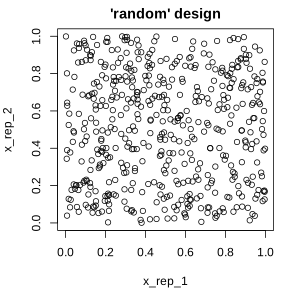
\includegraphics[width=0.45\linewidth]{06-technical-paradox_files/figure-latex/05-technical-paradox-023-1} 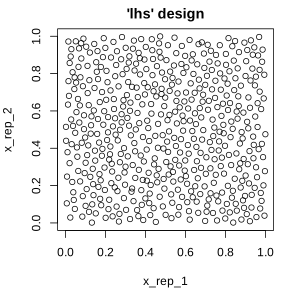
\includegraphics[width=0.45\linewidth]{06-technical-paradox_files/figure-latex/05-technical-paradox-023-2} \end{center}

\hypertarget{generalized-sampling-the-sampler-class}{%
\subsubsection{\texorpdfstring{Generalized Sampling: The \texttt{Sampler} Class}{Generalized Sampling: The Sampler Class}}\label{generalized-sampling-the-sampler-class}}

It may sometimes be desirable to configure parameter sampling in more detail.
\texttt{paradox} uses the \texttt{Sampler} abstract base class for sampling, which has many different sub-classes that can be parameterized and combined to control the sampling process.
It is even possible to create further sub-classes of the \texttt{Sampler} class (or of any of \emph{its} subclasses) for even more possibilities.

Every \texttt{Sampler} object has a \texttt{sample()} function, which takes one argument, the number of instances to sample, and returns a \protect\hyperlink{parameter-designs}{\texttt{Design}} object.

\hypertarget{d-samplers}{%
\paragraph{1D-Samplers}\label{d-samplers}}

There is a variety of samplers that sample values for a single parameter.
These are \texttt{Sampler1DUnif} (uniform sampling), \texttt{Sampler1DCateg} (sampling for categorical parameters), \texttt{Sampler1DNormal} (normally distributed sampling, truncated at parameter bounds), and \texttt{Sampler1DRfun} (arbitrary 1D sampling, given a random-function).
These are initialized with a single \texttt{Param}, and can then be used to sample values.

\begin{Shaded}
\begin{Highlighting}[]
\NormalTok{sampA }\OtherTok{=}\NormalTok{ Sampler1DCateg}\SpecialCharTok{$}\FunctionTok{new}\NormalTok{(parA)}
\NormalTok{sampA}\SpecialCharTok{$}\FunctionTok{sample}\NormalTok{(}\DecValTok{5}\NormalTok{)}
\end{Highlighting}
\end{Shaded}

\begin{verbatim}
## <Design> with 5 rows:
##        A
## 1:  TRUE
## 2:  TRUE
## 3: FALSE
## 4: FALSE
## 5:  TRUE
\end{verbatim}

\hypertarget{hierarchical-sampler}{%
\paragraph{Hierarchical Sampler}\label{hierarchical-sampler}}

The \texttt{SamplerHierarchical} sampler is an auxiliary sampler that combines many 1D-Samplers to get a combined distribution.
Its name ``hierarchical'' implies that it is able to respect parameter dependencies.
This suggests that parameters only get sampled when their dependencies are met.

The following example shows how this works: The \texttt{Int} parameter \texttt{B} depends on the \texttt{Lgl} parameter \texttt{A} being \texttt{TRUE}.
\texttt{A} is sampled to be \texttt{TRUE} in about half the cases, in which case \texttt{B} takes a value between 0 and 10.
In the cases where \texttt{A} is \texttt{FALSE}, \texttt{B} is set to \texttt{NA}.

\begin{Shaded}
\begin{Highlighting}[]
\NormalTok{psSmall}\SpecialCharTok{$}\FunctionTok{add\_dep}\NormalTok{(}\StringTok{"B"}\NormalTok{, }\StringTok{"A"}\NormalTok{, CondEqual}\SpecialCharTok{$}\FunctionTok{new}\NormalTok{(}\ConstantTok{TRUE}\NormalTok{))}
\NormalTok{sampH }\OtherTok{=}\NormalTok{ SamplerHierarchical}\SpecialCharTok{$}\FunctionTok{new}\NormalTok{(psSmall,}
  \FunctionTok{list}\NormalTok{(Sampler1DCateg}\SpecialCharTok{$}\FunctionTok{new}\NormalTok{(parA),}
\NormalTok{    Sampler1DUnif}\SpecialCharTok{$}\FunctionTok{new}\NormalTok{(parB),}
\NormalTok{    Sampler1DUnif}\SpecialCharTok{$}\FunctionTok{new}\NormalTok{(parC))}
\NormalTok{)}
\NormalTok{sampled }\OtherTok{=}\NormalTok{ sampH}\SpecialCharTok{$}\FunctionTok{sample}\NormalTok{(}\DecValTok{1000}\NormalTok{)}
\FunctionTok{table}\NormalTok{(sampled}\SpecialCharTok{$}\NormalTok{data[, }\FunctionTok{c}\NormalTok{(}\StringTok{"A"}\NormalTok{, }\StringTok{"B"}\NormalTok{)], }\AttributeTok{useNA =} \StringTok{"ifany"}\NormalTok{)}
\end{Highlighting}
\end{Shaded}

\begin{verbatim}
##        B
## A         0   1   2   3   4   5   6   7   8   9  10 <NA>
##   FALSE   0   0   0   0   0   0   0   0   0   0   0  487
##   TRUE   46  41  47  56  50  42  49  48  45  47  42    0
\end{verbatim}

\hypertarget{joint-sampler}{%
\paragraph{Joint Sampler}\label{joint-sampler}}

Another way of combining samplers is the \texttt{SamplerJointIndep}.
\texttt{SamplerJointIndep} also makes it possible to combine \texttt{Sampler}s that are not 1D.
However, \texttt{SamplerJointIndep} currently can not handle \texttt{ParamSet}s with dependencies.

\begin{Shaded}
\begin{Highlighting}[]
\NormalTok{sampJ }\OtherTok{=}\NormalTok{ SamplerJointIndep}\SpecialCharTok{$}\FunctionTok{new}\NormalTok{(}
  \FunctionTok{list}\NormalTok{(Sampler1DUnif}\SpecialCharTok{$}\FunctionTok{new}\NormalTok{(ParamDbl}\SpecialCharTok{$}\FunctionTok{new}\NormalTok{(}\StringTok{"x"}\NormalTok{, }\DecValTok{0}\NormalTok{, }\DecValTok{1}\NormalTok{)),}
\NormalTok{    Sampler1DUnif}\SpecialCharTok{$}\FunctionTok{new}\NormalTok{(ParamDbl}\SpecialCharTok{$}\FunctionTok{new}\NormalTok{(}\StringTok{"y"}\NormalTok{, }\DecValTok{0}\NormalTok{, }\DecValTok{1}\NormalTok{)))}
\NormalTok{)}
\NormalTok{sampJ}\SpecialCharTok{$}\FunctionTok{sample}\NormalTok{(}\DecValTok{5}\NormalTok{)}
\end{Highlighting}
\end{Shaded}

\begin{verbatim}
## <Design> with 5 rows:
##         x       y
## 1: 0.3508 0.78770
## 2: 0.2547 0.07967
## 3: 0.6562 0.10313
## 4: 0.9719 0.03180
## 5: 0.6477 0.56455
\end{verbatim}

\hypertarget{samplerunif}{%
\paragraph{SamplerUnif}\label{samplerunif}}

The \texttt{Sampler} used in \texttt{generate\_design\_random} is the \texttt{SamplerUnif} sampler, which corresponds to a \texttt{HierarchicalSampler} of \texttt{Sampler1DUnif} for all parameters.

\hypertarget{parameter-transformation}{%
\subsection{Parameter Transformation}\label{parameter-transformation}}

While the different \texttt{Sampler}s allow for a wide specification of parameter distributions, there are cases where the simplest way of getting a desired distribution is to sample parameters from a simple distribution (such as the uniform distribution) and then transform them.
This can be done by assigning a function to the \texttt{\$trafo} slot of a \texttt{ParamSet}.
The \texttt{\$trafo} function is called with two parameters:

\begin{itemize}
\tightlist
\item
  The list of parameter values to be transformed as \texttt{x}
\item
  The \texttt{ParamSet} itself as \texttt{param\_set}
\end{itemize}

The \texttt{\$trafo} function must return a list of transformed parameter values.

The transformation is performed when calling the \texttt{\$transpose} function of the \texttt{Design} object returned by a \texttt{Sampler} with the \texttt{trafo} ParamSet to \texttt{TRUE} (the default).
The following, for example, creates a parameter that is exponentially distributed:

\begin{Shaded}
\begin{Highlighting}[]
\NormalTok{psexp }\OtherTok{=}\NormalTok{ ParamSet}\SpecialCharTok{$}\FunctionTok{new}\NormalTok{(}\FunctionTok{list}\NormalTok{(ParamDbl}\SpecialCharTok{$}\FunctionTok{new}\NormalTok{(}\StringTok{"par"}\NormalTok{, }\DecValTok{0}\NormalTok{, }\DecValTok{1}\NormalTok{)))}
\NormalTok{psexp}\SpecialCharTok{$}\NormalTok{trafo }\OtherTok{=} \ControlFlowTok{function}\NormalTok{(x, param\_set) \{}
\NormalTok{  x}\SpecialCharTok{$}\NormalTok{par }\OtherTok{=} \SpecialCharTok{{-}}\FunctionTok{log}\NormalTok{(x}\SpecialCharTok{$}\NormalTok{par)}
\NormalTok{  x}
\NormalTok{\}}
\NormalTok{design }\OtherTok{=} \FunctionTok{generate\_design\_random}\NormalTok{(psexp, }\DecValTok{2}\NormalTok{)}
\FunctionTok{print}\NormalTok{(design)}
\end{Highlighting}
\end{Shaded}

\begin{verbatim}
## <Design> with 2 rows:
##        par
## 1: 0.05488
## 2: 0.37323
\end{verbatim}

\begin{Shaded}
\begin{Highlighting}[]
\NormalTok{design}\SpecialCharTok{$}\FunctionTok{transpose}\NormalTok{()  }\CommentTok{\# trafo is TRUE}
\end{Highlighting}
\end{Shaded}

\begin{verbatim}
## [[1]]
## [[1]]$par
## [1] 2.903
## 
## 
## [[2]]
## [[2]]$par
## [1] 0.9856
\end{verbatim}

Compare this to \texttt{\$transpose()} without transformation:

\begin{Shaded}
\begin{Highlighting}[]
\NormalTok{design}\SpecialCharTok{$}\FunctionTok{transpose}\NormalTok{(}\AttributeTok{trafo =} \ConstantTok{FALSE}\NormalTok{)}
\end{Highlighting}
\end{Shaded}

\begin{verbatim}
## [[1]]
## [[1]]$par
## [1] 0.05488
## 
## 
## [[2]]
## [[2]]$par
## [1] 0.3732
\end{verbatim}

\hypertarget{transformation-between-types}{%
\subsubsection{Transformation between Types}\label{transformation-between-types}}

Usually the design created with one \texttt{ParamSet} is then used to configure other objects that themselves have a \texttt{ParamSet} which defines the values they take.
The \texttt{ParamSet}s which can be used for random sampling, however, are restricted in some ways:
They must have finite bounds, and they may not contain ``untyped'' (\texttt{ParamUty}) parameters.
\texttt{\$trafo} provides the glue for these situations.
There is relatively little constraint on the trafo function's return value, so it is possible to return values that have different bounds or even types than the original \texttt{ParamSet}.
It is even possible to remove some parameters and add new ones.

Suppose, for example, that a certain method requires a \emph{function} as a parameter.
Let's say a function that summarizes its data in a certain way.
The user can pass functions like \texttt{median()} or \texttt{mean()}, but could also pass quantiles or something completely different.
This method would probably use the following \texttt{ParamSet}:

\begin{Shaded}
\begin{Highlighting}[]
\NormalTok{methodPS }\OtherTok{=}\NormalTok{ ParamSet}\SpecialCharTok{$}\FunctionTok{new}\NormalTok{(}
  \FunctionTok{list}\NormalTok{(}
\NormalTok{    ParamUty}\SpecialCharTok{$}\FunctionTok{new}\NormalTok{(}\StringTok{"fun"}\NormalTok{,}
      \AttributeTok{custom\_check =} \ControlFlowTok{function}\NormalTok{(x) checkmate}\SpecialCharTok{::}\FunctionTok{checkFunction}\NormalTok{(x, }\AttributeTok{nargs =} \DecValTok{1}\NormalTok{))}
\NormalTok{  )}
\NormalTok{)}
\FunctionTok{print}\NormalTok{(methodPS)}
\end{Highlighting}
\end{Shaded}

\begin{verbatim}
## <ParamSet>
##     id    class lower upper nlevels        default value
## 1: fun ParamUty    NA    NA     Inf <NoDefault[3]>
\end{verbatim}

If one wanted to sample this method, using one of four functions, a way to do this would be:

\begin{Shaded}
\begin{Highlighting}[]
\NormalTok{samplingPS }\OtherTok{=}\NormalTok{ ParamSet}\SpecialCharTok{$}\FunctionTok{new}\NormalTok{(}
  \FunctionTok{list}\NormalTok{(}
\NormalTok{    ParamFct}\SpecialCharTok{$}\FunctionTok{new}\NormalTok{(}\StringTok{"fun"}\NormalTok{, }\FunctionTok{c}\NormalTok{(}\StringTok{"mean"}\NormalTok{, }\StringTok{"median"}\NormalTok{, }\StringTok{"min"}\NormalTok{, }\StringTok{"max"}\NormalTok{))}
\NormalTok{  )}
\NormalTok{)}

\NormalTok{samplingPS}\SpecialCharTok{$}\NormalTok{trafo }\OtherTok{=} \ControlFlowTok{function}\NormalTok{(x, param\_set) \{}
  \CommentTok{\# x$fun is a \textasciigrave{}character(1)\textasciigrave{},}
  \CommentTok{\# in particular one of \textquotesingle{}mean\textquotesingle{}, \textquotesingle{}median\textquotesingle{}, \textquotesingle{}min\textquotesingle{}, \textquotesingle{}max\textquotesingle{}.}
  \CommentTok{\# We want to turn it into a function!}
\NormalTok{  x}\SpecialCharTok{$}\NormalTok{fun }\OtherTok{=} \FunctionTok{get}\NormalTok{(x}\SpecialCharTok{$}\NormalTok{fun, }\AttributeTok{mode =} \StringTok{"function"}\NormalTok{)}
\NormalTok{  x}
\NormalTok{\}}
\end{Highlighting}
\end{Shaded}

\begin{Shaded}
\begin{Highlighting}[]
\NormalTok{design }\OtherTok{=} \FunctionTok{generate\_design\_random}\NormalTok{(samplingPS, }\DecValTok{2}\NormalTok{)}
\FunctionTok{print}\NormalTok{(design)}
\end{Highlighting}
\end{Shaded}

\begin{verbatim}
## <Design> with 2 rows:
##       fun
## 1: median
## 2:    min
\end{verbatim}

Note that the \texttt{Design} only contains the column ``\texttt{fun}'' as a \texttt{character} column.
To get a single value as a \emph{function}, the \texttt{\$transpose} function is used.

\begin{Shaded}
\begin{Highlighting}[]
\NormalTok{xvals }\OtherTok{=}\NormalTok{ design}\SpecialCharTok{$}\FunctionTok{transpose}\NormalTok{()}
\FunctionTok{print}\NormalTok{(xvals[[}\DecValTok{1}\NormalTok{]])}
\end{Highlighting}
\end{Shaded}

\begin{verbatim}
## $fun
## function (x, na.rm = FALSE, ...) 
## UseMethod("median")
## <bytecode: 0x558bf68478a0>
## <environment: namespace:stats>
\end{verbatim}

We can now check that it fits the requirements set by \texttt{methodPS}, and that \texttt{fun} it is in fact a function:

\begin{Shaded}
\begin{Highlighting}[]
\NormalTok{methodPS}\SpecialCharTok{$}\FunctionTok{check}\NormalTok{(xvals[[}\DecValTok{1}\NormalTok{]])}
\end{Highlighting}
\end{Shaded}

\begin{verbatim}
## [1] "fun: Must have exactly 1 formal arguments, but has 2"
\end{verbatim}

\begin{Shaded}
\begin{Highlighting}[]
\NormalTok{xvals[[}\DecValTok{1}\NormalTok{]]}\SpecialCharTok{$}\FunctionTok{fun}\NormalTok{(}\DecValTok{1}\SpecialCharTok{:}\DecValTok{10}\NormalTok{)}
\end{Highlighting}
\end{Shaded}

\begin{verbatim}
## [1] 5.5
\end{verbatim}

Imagine now that a different kind of parametrization of the function is desired:
The user wants to give a function that selects a certain quantile, where the quantile is set by a parameter.
In that case the \texttt{\$transpose} function could generate a function in a different way.
For interpretability, the parameter is called ``\texttt{quantile}'' before transformation, and the ``\texttt{fun}'' parameter is generated on the fly.

\begin{Shaded}
\begin{Highlighting}[]
\NormalTok{samplingPS2 }\OtherTok{=}\NormalTok{ ParamSet}\SpecialCharTok{$}\FunctionTok{new}\NormalTok{(}
  \FunctionTok{list}\NormalTok{(}
\NormalTok{    ParamDbl}\SpecialCharTok{$}\FunctionTok{new}\NormalTok{(}\StringTok{"quantile"}\NormalTok{, }\DecValTok{0}\NormalTok{, }\DecValTok{1}\NormalTok{)}
\NormalTok{  )}
\NormalTok{)}

\NormalTok{samplingPS2}\SpecialCharTok{$}\NormalTok{trafo }\OtherTok{=} \ControlFlowTok{function}\NormalTok{(x, param\_set) \{}
  \CommentTok{\# x$quantile is a \textasciigrave{}numeric(1)\textasciigrave{} between 0 and 1.}
  \CommentTok{\# We want to turn it into a function!}
  \FunctionTok{list}\NormalTok{(}\AttributeTok{fun =} \ControlFlowTok{function}\NormalTok{(input) }\FunctionTok{quantile}\NormalTok{(input, x}\SpecialCharTok{$}\NormalTok{quantile))}
\NormalTok{\}}
\end{Highlighting}
\end{Shaded}

\begin{Shaded}
\begin{Highlighting}[]
\NormalTok{design }\OtherTok{=} \FunctionTok{generate\_design\_random}\NormalTok{(samplingPS2, }\DecValTok{2}\NormalTok{)}
\FunctionTok{print}\NormalTok{(design)}
\end{Highlighting}
\end{Shaded}

\begin{verbatim}
## <Design> with 2 rows:
##    quantile
## 1:   0.7855
## 2:   0.1431
\end{verbatim}

The \texttt{Design} now contains the column ``\texttt{quantile}'' that will be used by the \texttt{\$transpose} function to create the \texttt{fun} parameter.
We also check that it fits the requirement set by \texttt{methodPS}, and that it is a function.

\begin{Shaded}
\begin{Highlighting}[]
\NormalTok{xvals }\OtherTok{=}\NormalTok{ design}\SpecialCharTok{$}\FunctionTok{transpose}\NormalTok{()}
\FunctionTok{print}\NormalTok{(xvals[[}\DecValTok{1}\NormalTok{]])}
\end{Highlighting}
\end{Shaded}

\begin{verbatim}
## $fun
## function(input) quantile(input, x$quantile)
## <environment: 0x558bfa4f4ae8>
\end{verbatim}

\begin{Shaded}
\begin{Highlighting}[]
\NormalTok{methodPS}\SpecialCharTok{$}\FunctionTok{check}\NormalTok{(xvals[[}\DecValTok{1}\NormalTok{]])}
\end{Highlighting}
\end{Shaded}

\begin{verbatim}
## [1] TRUE
\end{verbatim}

\begin{Shaded}
\begin{Highlighting}[]
\NormalTok{xvals[[}\DecValTok{1}\NormalTok{]]}\SpecialCharTok{$}\FunctionTok{fun}\NormalTok{(}\DecValTok{1}\SpecialCharTok{:}\DecValTok{10}\NormalTok{)}
\end{Highlighting}
\end{Shaded}

\begin{verbatim}
## 78.54963% 
##     8.069
\end{verbatim}

\hypertarget{logging}{%
\section{Logging}\label{logging}}

We use the \href{https://cran.r-project.org/package=lgr}{lgr} package for logging and progress output.

\hypertarget{changing-mlr3-logging-levels}{%
\subsection{Changing mlr3 logging levels}\label{changing-mlr3-logging-levels}}

To change the setting for \href{https://mlr3.mlr-org.com}{mlr3} for the current session, you need to retrieve the logger (which is a \href{https://cran.r-project.org/package=R6}{R6} object) from \href{https://cran.r-project.org/package=lgr}{lgr}, and then change the threshold of the like this:

\begin{Shaded}
\begin{Highlighting}[]
\FunctionTok{requireNamespace}\NormalTok{(}\StringTok{"lgr"}\NormalTok{)}

\NormalTok{logger }\OtherTok{=}\NormalTok{ lgr}\SpecialCharTok{::}\FunctionTok{get\_logger}\NormalTok{(}\StringTok{"mlr3"}\NormalTok{)}
\NormalTok{logger}\SpecialCharTok{$}\FunctionTok{set\_threshold}\NormalTok{(}\StringTok{"\textless{}level\textgreater{}"}\NormalTok{)}
\end{Highlighting}
\end{Shaded}

The default log level is \texttt{"info"}.
All available levels can be listed as follows:

\begin{Shaded}
\begin{Highlighting}[]
\FunctionTok{getOption}\NormalTok{(}\StringTok{"lgr.log\_levels"}\NormalTok{)}
\end{Highlighting}
\end{Shaded}

\begin{verbatim}
## fatal error  warn  info debug trace 
##   100   200   300   400   500   600
\end{verbatim}

To increase verbosity, set the log level to a higher value, e.g.~to \texttt{"debug"} with:

\begin{Shaded}
\begin{Highlighting}[]
\NormalTok{lgr}\SpecialCharTok{::}\FunctionTok{get\_logger}\NormalTok{(}\StringTok{"mlr3"}\NormalTok{)}\SpecialCharTok{$}\FunctionTok{set\_threshold}\NormalTok{(}\StringTok{"debug"}\NormalTok{)}
\end{Highlighting}
\end{Shaded}

To reduce the verbosity, reduce the log level to warn:

\begin{Shaded}
\begin{Highlighting}[]
\NormalTok{lgr}\SpecialCharTok{::}\FunctionTok{get\_logger}\NormalTok{(}\StringTok{"mlr3"}\NormalTok{)}\SpecialCharTok{$}\FunctionTok{set\_threshold}\NormalTok{(}\StringTok{"warn"}\NormalTok{)}
\end{Highlighting}
\end{Shaded}

\href{https://cran.r-project.org/package=lgr}{lgr} comes with a global option called \texttt{"lgr.default\_threshold"} which can be set via \texttt{options()} to make your choice permanent across sessions.

Also note that the optimization packages such as \href{https://mlr3tuning.mlr-org.com}{mlr3tuning} \href{https://mlr3fselect.mlr-org.com}{mlr3fselect} use the logger of their base package \href{https://bbotk.mlr-org.com}{bbotk}.
To disable the output from \href{https://mlr3.mlr-org.com}{mlr3}, but keep the output from \href{https://mlr3tuning.mlr-org.com}{mlr3tuning}, reduce the verbosity for the logger \href{https://mlr3.mlr-org.com}{mlr3}
and optionally change the logger \href{https://bbotk.mlr-org.com}{bbotk} to the desired level.

\begin{Shaded}
\begin{Highlighting}[]
\NormalTok{lgr}\SpecialCharTok{::}\FunctionTok{get\_logger}\NormalTok{(}\StringTok{"mlr3"}\NormalTok{)}\SpecialCharTok{$}\FunctionTok{set\_threshold}\NormalTok{(}\StringTok{"warn"}\NormalTok{)}
\NormalTok{lgr}\SpecialCharTok{::}\FunctionTok{get\_logger}\NormalTok{(}\StringTok{"bbotk"}\NormalTok{)}\SpecialCharTok{$}\FunctionTok{set\_threshold}\NormalTok{(}\StringTok{"info"}\NormalTok{)}
\end{Highlighting}
\end{Shaded}

\hypertarget{redirecting-output}{%
\subsection{Redirecting output}\label{redirecting-output}}

Redirecting output is already extensively covered in the documentation and vignette of \href{https://cran.r-project.org/package=lgr}{lgr}.
Here is just a short example which adds an additional appender to log events into a temporary file in \href{https://en.wikipedia.org/wiki/JSON}{JSON} format:

\begin{Shaded}
\begin{Highlighting}[]
\NormalTok{tf }\OtherTok{=} \FunctionTok{tempfile}\NormalTok{(}\StringTok{"mlr3log\_"}\NormalTok{, }\AttributeTok{fileext =} \StringTok{".json"}\NormalTok{)}

\CommentTok{\# get the logger as R6 object}
\NormalTok{logger }\OtherTok{=}\NormalTok{ lgr}\SpecialCharTok{::}\FunctionTok{get\_logger}\NormalTok{(}\StringTok{"mlr"}\NormalTok{)}

\CommentTok{\# add Json appender}
\NormalTok{logger}\SpecialCharTok{$}\FunctionTok{add\_appender}\NormalTok{(lgr}\SpecialCharTok{::}\NormalTok{AppenderJson}\SpecialCharTok{$}\FunctionTok{new}\NormalTok{(tf), }\AttributeTok{name =} \StringTok{"json"}\NormalTok{)}

\CommentTok{\# signal a warning}
\NormalTok{logger}\SpecialCharTok{$}\FunctionTok{warn}\NormalTok{(}\StringTok{"this is a warning from mlr3"}\NormalTok{)}

\CommentTok{\# print the contents of the file}
\FunctionTok{cat}\NormalTok{(}\FunctionTok{readLines}\NormalTok{(tf))}

\CommentTok{\# remove the appender again}
\NormalTok{logger}\SpecialCharTok{$}\FunctionTok{remove\_appender}\NormalTok{(}\StringTok{"json"}\NormalTok{)}
\end{Highlighting}
\end{Shaded}

\hypertarget{immediate-log-feedback}{%
\subsection{Immediate Log Feedback}\label{immediate-log-feedback}}

\href{https://mlr3.mlr-org.com}{mlr3} uses the \protect\hyperlink{parallelization}{future} package and \protect\hyperlink{encapsulation}{encapsulation} to make evaluations fast, stable, and reproducible.
However, this may lead to logs being delayed, out of order, or, in case of some errors, not present at all.
When it is necessary to have immediate access to log messages, for example to investigate problems, one may therefore choose to disable \href{https://cran.r-project.org/package=future}{future} and encapsulation.
This can be done by enabling the debug mode using \texttt{options(mlr.debug\ =\ TRUE)}; the \texttt{\$encapsulate} slot of learners should also be set to \texttt{"none"} (default) or \texttt{"evaluate"}, but not \texttt{"callr"}.
This should only be done to investigate problems, however, and not for production use, because (1) this disables parallelization, and (2) this leads to different RNG behavior and therefore to results that are not reproducible when the debug mode is not set.

\hypertarget{extending}{%
\chapter{Extending}\label{extending}}

This chapter gives instructions on how to extend \href{https://mlr3.mlr-org.com}{mlr3} and its extension packages with custom objects.

The approach is always the same:

\begin{enumerate}
\def\labelenumi{\arabic{enumi}.}
\tightlist
\item
  determine the base class you want to inherit from,
\item
  extend the class with your custom functionality,
\item
  test your implementation
\item
  (optionally) add new object to the respective \href{https://mlr3misc.mlr-org.com/reference/Dictionary.html}{\texttt{Dictionary}}.
\end{enumerate}

The chapter \protect\hyperlink{extending-learners}{Create a new learner} illustrates the steps needed to create a custom learner in \href{https://mlr3.mlr-org.com}{mlr3}.

\hypertarget{extending-learners}{%
\section{Adding new Learners}\label{extending-learners}}

Here, we show how to create a custom mlr3learner step-by-step using \href{https://mlr3extralearners.mlr-org.com/reference/create_learner.html}{\texttt{mlr3extralearners::create\_learner}}.

\textbf{It is strongly recommended} that you \textbf{first} open a \href{https://github.com/mlr-org/mlr3extralearners/issues/new?assignees=\&labels=new+learner\&template=learner-request-template.md\&title=\%5BLRNRQ\%5D+Add+\%3Calgorithm\%3E+from+package+\%3Cpackage\%3E}{learner request issue} to discuss the learner you want to implement if you plan on creating a pull request to the mlr-org. This allows us to discuss the purpose and necessity of the learner before you start to put the real work in!

This section gives insights on how a mlr3learner is constructed and how to troubleshoot issues.
See the \protect\hyperlink{learner-faq}{Learner FAQ subsection} for help.

\textbf{Summary of steps for adding a new learner}

\begin{enumerate}
\def\labelenumi{\arabic{enumi}.}
\tightlist
\item
  Check the learner does not already exist \href{https://mlr3extralearners.mlr-org.com/articles/learners/list_learners.html}{here}.
\item
  \protect\hyperlink{setup}{Fork, clone and load} \texttt{mlr3extralearners}.
\item
  \protect\hyperlink{create-learner}{Run} \href{https://mlr3extralearners.mlr-org.com/reference/create_learner.html}{\texttt{mlr3extralearners::create\_learner}}.
\item
  Add the learner \protect\hyperlink{param-set}{\texttt{param\_set}}.
\item
  Manually add \protect\hyperlink{learner-train}{\texttt{.train}} and \protect\hyperlink{learner-predict}{\texttt{.predict}} private methods to the learner.
\item
  If applicable add \texttt{importance} and \texttt{oob\_error} public methods to the learner.
\item
  If applicable add references to the learner.
\item
  Check \protect\hyperlink{learner-test}{unit tests} and \protect\hyperlink{learner-test}{paramtests} pass (these are automatically created).
\item
  Run \protect\hyperlink{cleaning}{cleaning functions}
\item
  Open a \href{https://github.com/mlr-org/mlr3extralearners/pulls}{pull request} with the new learner template.
\end{enumerate}

\textbf{(Do not copy/paste the code shown in this section. Use the create\_learner to start.)}

\hypertarget{setup}{%
\subsection{Setting-up mlr3extralearners}\label{setup}}

In order to use the \href{https://mlr3extralearners.mlr-org.com/reference/create_learner.html}{\texttt{mlr3extralearners::create\_learner}} function you must have a local copy of the \texttt{mlr3extralearners} repository and must specify the correct path to the package. To do so, follow these steps:

\begin{enumerate}
\def\labelenumi{\arabic{enumi}.}
\tightlist
\item
  \href{https://docs.github.com/en/free-pro-team@latest/github/getting-started-with-github/fork-a-repo}{Fork} the \href{https://github.com/mlr-org/mlr3extralearners}{repository}
\item
  \href{https://docs.github.com/en/free-pro-team@latest/github/creating-cloning-and-archiving-repositories/cloning-a-repository}{Clone} a local copy of your forked repository.
\end{enumerate}

Then do one of:

\begin{itemize}
\tightlist
\item
  Open a new R session, call \texttt{library("mlr3extralearners")} (install if you haven't already), and then \protect\hyperlink{create-learner}{run} \href{https://mlr3extralearners.mlr-org.com/reference/create_learner.html}{\texttt{mlr3extralearners::create\_learner}} with the \texttt{pkg} argument set as the path (the folder location) to the package directory.
\item
  Open a new R session, set your working directory as your newly cloned repository, run \href{https://www.rdocumentation.org/packages/devtools/topics/load_all}{\texttt{devtools::load\_all}}, and then \protect\hyperlink{create-learner}{run} \href{https://mlr3extralearners.mlr-org.com/reference/create_learner.html}{\texttt{mlr3extralearners::create\_learner}}, leaving \texttt{pkg\ =\ "."}.
\item
  In your newly cloned repository, open the R project, which will automatically set your working directory, run \href{https://www.rdocumentation.org/packages/devtools/topics/load_all}{\texttt{devtools::load\_all}}, and then \protect\hyperlink{create-learner}{run} \href{https://mlr3extralearners.mlr-org.com/reference/create_learner.html}{\texttt{mlr3extralearners::create\_learner}}, leaving \texttt{pkg\ =\ "."}.
\end{itemize}

We recommend the last option. It is also important that you are familiar with the three \texttt{devtools} commands:

\begin{itemize}
\tightlist
\item
  \href{https://www.rdocumentation.org/packages/devtools/topics/document}{\texttt{devtools::document}} - Generates roxygen documentation for your new learner.
\item
  \href{https://www.rdocumentation.org/packages/devtools/topics/load_all}{\texttt{devtools::load\_all}} - Loads all functions from \texttt{mlr3extralearners} locally, including hidden helper functions.
\item
  \href{https://www.rdocumentation.org/packages/devtools/topics/check}{\texttt{devtools::check}} - Checks that the package still passes all tests locally.
\end{itemize}

\hypertarget{create-learner}{%
\subsection{Calling create\_learner}\label{create-learner}}

The learner \texttt{classif.rpart} will be used as a running example throughout this section.

\begin{Shaded}
\begin{Highlighting}[]
\FunctionTok{library}\NormalTok{(}\StringTok{"mlr3extralearners"}\NormalTok{)}
\FunctionTok{create\_learner}\NormalTok{(}
  \AttributeTok{pkg =} \StringTok{"."}\NormalTok{,}
  \AttributeTok{classname =} \StringTok{"Rpart"}\NormalTok{,}
  \AttributeTok{algorithm =} \StringTok{"decision tree"}\NormalTok{,}
  \AttributeTok{type =} \StringTok{"classif"}\NormalTok{,}
  \AttributeTok{key =} \StringTok{"rpart"}\NormalTok{,}
  \AttributeTok{package =} \StringTok{"rpart"}\NormalTok{,}
  \AttributeTok{caller =} \StringTok{"rpart"}\NormalTok{,}
  \AttributeTok{feature\_types =} \FunctionTok{c}\NormalTok{(}\StringTok{"logical"}\NormalTok{, }\StringTok{"integer"}\NormalTok{, }\StringTok{"numeric"}\NormalTok{, }\StringTok{"factor"}\NormalTok{, }\StringTok{"ordered"}\NormalTok{),}
  \AttributeTok{predict\_types =} \FunctionTok{c}\NormalTok{(}\StringTok{"response"}\NormalTok{, }\StringTok{"prob"}\NormalTok{),}
  \AttributeTok{properties =} \FunctionTok{c}\NormalTok{(}\StringTok{"importance"}\NormalTok{, }\StringTok{"missings"}\NormalTok{, }\StringTok{"multiclass"}\NormalTok{, }\StringTok{"selected\_features"}\NormalTok{, }\StringTok{"twoclass"}\NormalTok{, }\StringTok{"weights"}\NormalTok{),}
  \AttributeTok{references =} \ConstantTok{TRUE}\NormalTok{,}
  \AttributeTok{gh\_name =} \StringTok{"RaphaelS1"}
\NormalTok{)}
\end{Highlighting}
\end{Shaded}

The full documentation for the function arguments is in \href{https://mlr3extralearners.mlr-org.com/reference/create_learner.html}{\texttt{mlr3extralearners::create\_learner}}, in this example we are doing the following:

\begin{enumerate}
\def\labelenumi{\arabic{enumi}.}
\tightlist
\item
  \texttt{pkg\ =\ "."} - Set the package root to the current directory (assumes \texttt{mlr3extralearners} already set as the working directory)
\item
  \texttt{classname\ =\ "Rpart"} - Set the R6 class name to LearnerClassifRpart (classif is below)
\item
  \texttt{algorithm\ =\ "decision\ tree"} - Create the title as ``Classification Decision Tree Learner'', where ``Classification'' is determined automatically from \texttt{type} and ``Learner'' is added for all learners.
\item
  \texttt{type\ =\ "classif"} - Setting the learner as a classification learner, automatically filling the title, class name, id (``classif.rpart'') and task type.
\item
  \texttt{key\ =\ "rpart"} - Used with \texttt{type} to create the unique ID of the learner, \texttt{classif.rpart}.
\item
  \texttt{package\ =\ "rpart"} - Setting the package from which the learner is implemented, this fills in things like the training function (along with \texttt{caller}) and the \texttt{man} field.
\item
  \texttt{caller\ =\ "rpart"} - This tells the \texttt{.train} function, and the description which function is called to run the algorithm, with \texttt{package} this automatically fills \texttt{rpart::rpart}.
\item
  \texttt{feature\_types\ =\ c("logical",\ "integer",\ "numeric",\ "factor",\ "ordered")} - Sets the type of features that can be handled by the learner. See \protect\hyperlink{learner-meta-information}{meta information}.
\item
  \texttt{predict\_types\ =\ c("response",\ "prob"),} - Sets the possible prediction types as response (deterministic) and prob (probabilistic). See \protect\hyperlink{learner-meta-information}{meta information}.
\item
  \texttt{properties\ =\ c("importance",\ "missings",\ "multiclass",\ "selected\_features",\ "twoclass",\ "weights")} - Sets the properties that are handled by the learner, by including \texttt{"importance"} a public method called \texttt{importance} will be created that must be manually filled. See \protect\hyperlink{learner-meta-information}{meta information}.
\item
  \texttt{references\ =\ TRUE} - Tells the template to add a ``references'' tag that must be filled manually.
\item
  \texttt{gh\_name\ =\ "RaphaelS1"} - Fills the ``author'' tag with my GitHub handle, this is required as it identifies the maintainer of the learner.
\end{enumerate}

The sections below demonstrate what happens after the function has been run and the files that are created.

\hypertarget{learner_package_type_key.r}{%
\subsection{learner\_package\_type\_key.R}\label{learner_package_type_key.r}}

The first script to complete after running \texttt{create\_learner} is the file with the form \texttt{learner\_package\_type\_key.R}, in our case this will actually be \texttt{learner\_rpart\_classif\_rpart.key}. \textbf{This name must not be changed} as triggering automated tests rely on a strict naming scheme. For our example, the resulting script looks like this:

\begin{Shaded}
\begin{Highlighting}[]
\CommentTok{\#\textquotesingle{} @title Classification Decision Tree Learner}
\CommentTok{\#\textquotesingle{} @author RaphaelS1}
\CommentTok{\#\textquotesingle{} @name mlr\_learners\_classif.rpart}
\CommentTok{\#\textquotesingle{}}
\CommentTok{\#\textquotesingle{} @template class\_learner}
\CommentTok{\#\textquotesingle{} @templateVar id classif.rpart}
\CommentTok{\#\textquotesingle{} @templateVar caller rpart}
\CommentTok{\#\textquotesingle{}}
\CommentTok{\#\textquotesingle{} @references}
\CommentTok{\#\textquotesingle{} \textless{}}\AlertTok{FIXME}\CommentTok{ {-} DELETE THIS AND LINE ABOVE IF OMITTED\textgreater{}}
\CommentTok{\#\textquotesingle{}}
\CommentTok{\#\textquotesingle{} @template seealso\_learner}
\CommentTok{\#\textquotesingle{} @template example}
\CommentTok{\#\textquotesingle{} @export}
\NormalTok{LearnerClassifRpart }\OtherTok{=} \FunctionTok{R6Class}\NormalTok{(}\StringTok{"LearnerClassifRpart"}\NormalTok{,}
  \AttributeTok{inherit =}\NormalTok{ LearnerClassif,}

  \AttributeTok{public =} \FunctionTok{list}\NormalTok{(}
    \CommentTok{\#\textquotesingle{} @description}
    \CommentTok{\#\textquotesingle{} Creates a new instance of this [R6][R6::R6Class] class.}
    \AttributeTok{initialize =} \ControlFlowTok{function}\NormalTok{() \{}
      \CommentTok{\# }\AlertTok{FIXME}\CommentTok{ {-} MANUALLY ADD PARAM\_SET BELOW AND THEN DELETE THIS LINE}
\NormalTok{      ps }\OtherTok{=} \ErrorTok{\textless{}}\NormalTok{param\_set}\SpecialCharTok{\textgreater{}}

      \CommentTok{\# }\AlertTok{FIXME}\CommentTok{ {-} MANUALLY UPDATE PARAM VALUES BELOW IF APPLICABLE THEN DELETE THIS LINE.}
      \CommentTok{\# OTHERWISE DELETE THIS AND LINE BELOW.}
\NormalTok{      ps}\SpecialCharTok{$}\NormalTok{values }\OtherTok{=} \FunctionTok{list}\NormalTok{(}\SpecialCharTok{\textless{}}\NormalTok{param\_vals}\SpecialCharTok{\textgreater{}}\NormalTok{)}

\NormalTok{      super}\SpecialCharTok{$}\FunctionTok{initialize}\NormalTok{(}
        \AttributeTok{id =} \StringTok{"classif.rpart"}\NormalTok{,}
        \AttributeTok{packages =} \StringTok{"rpart"}\NormalTok{,}
        \AttributeTok{feature\_types =} \FunctionTok{c}\NormalTok{(}\StringTok{"logical"}\NormalTok{, }\StringTok{"integer"}\NormalTok{, }\StringTok{"numeric"}\NormalTok{, }\StringTok{"factor"}\NormalTok{, }\StringTok{"ordered"}\NormalTok{),}
        \AttributeTok{predict\_types =} \FunctionTok{c}\NormalTok{(}\StringTok{"response"}\NormalTok{, }\StringTok{"prob"}\NormalTok{),}
        \AttributeTok{param\_set =}\NormalTok{ ps,}
        \AttributeTok{properties =} \FunctionTok{c}\NormalTok{(}\StringTok{"importance"}\NormalTok{, }\StringTok{"missings"}\NormalTok{, }\StringTok{"multiclass"}\NormalTok{, }\StringTok{"selected\_features"}\NormalTok{, }\StringTok{"twoclass"}\NormalTok{, }\StringTok{"weights"}\NormalTok{),}
        \AttributeTok{man =} \StringTok{"mlr3extralearners::mlr\_learners\_classif.rpart"}
\NormalTok{      )}
\NormalTok{    \},}

    \CommentTok{\# }\AlertTok{FIXME}\CommentTok{ {-} ADD IMPORTANCE METHOD HERE AND DELETE THIS LINE.}
    \CommentTok{\# \textless{}See LearnerRegrRandomForest for an example\textgreater{}}
    \CommentTok{\#\textquotesingle{} @description}
    \CommentTok{\#\textquotesingle{} The importance scores are extracted from the slot \textless{}}\AlertTok{FIXME}\CommentTok{\textgreater{}.}
    \CommentTok{\#\textquotesingle{} @return Named \textasciigrave{}numeric()\textasciigrave{}.}
    \AttributeTok{importance =} \ControlFlowTok{function}\NormalTok{() \{ \}}

\NormalTok{  ),}

  \AttributeTok{private =} \FunctionTok{list}\NormalTok{(}

    \AttributeTok{.train =} \ControlFlowTok{function}\NormalTok{(task) \{}
\NormalTok{      pars }\OtherTok{=}\NormalTok{ self}\SpecialCharTok{$}\NormalTok{param\_set}\SpecialCharTok{$}\FunctionTok{get\_values}\NormalTok{(}\AttributeTok{tags =} \StringTok{"train"}\NormalTok{)}

      \CommentTok{\# set column names to ensure consistency in fit and predict}
\NormalTok{      self}\SpecialCharTok{$}\NormalTok{state}\SpecialCharTok{$}\NormalTok{feature\_names }\OtherTok{=}\NormalTok{ task}\SpecialCharTok{$}\NormalTok{feature\_names}

      \CommentTok{\# }\AlertTok{FIXME}\CommentTok{ {-} \textless{}Create objects for the train call}
      \CommentTok{\# \textless{}At least "data" and "formula" are required\textgreater{}}
\NormalTok{      formula }\OtherTok{=}\NormalTok{ task}\SpecialCharTok{$}\FunctionTok{formula}\NormalTok{()}
\NormalTok{      data }\OtherTok{=}\NormalTok{ task}\SpecialCharTok{$}\FunctionTok{data}\NormalTok{()}

      \CommentTok{\# }\AlertTok{FIXME}\CommentTok{ {-} \textless{}here is space for some custom adjustments before proceeding to the}
      \CommentTok{\# train call. Check other learners for what can be done here\textgreater{}}

      \CommentTok{\# use the mlr3misc::invoke function (it\textquotesingle{}s similar to do.call())}
\NormalTok{      mlr3misc}\SpecialCharTok{::}\FunctionTok{invoke}\NormalTok{(rpart}\SpecialCharTok{::}\NormalTok{rpart,}
                       \AttributeTok{formula =}\NormalTok{ formula,}
                       \AttributeTok{data =}\NormalTok{ data,}
                       \AttributeTok{.args =}\NormalTok{ pars)}
\NormalTok{    \},}

    \AttributeTok{.predict =} \ControlFlowTok{function}\NormalTok{(task) \{}
      \CommentTok{\# get parameters with tag "predict"}
\NormalTok{      pars }\OtherTok{=}\NormalTok{ self}\SpecialCharTok{$}\NormalTok{param\_set}\SpecialCharTok{$}\FunctionTok{get\_values}\NormalTok{(}\AttributeTok{tags =} \StringTok{"predict"}\NormalTok{)}
      \CommentTok{\# get newdata}
\NormalTok{      newdata }\OtherTok{=}\NormalTok{ task}\SpecialCharTok{$}\FunctionTok{data}\NormalTok{(}\AttributeTok{cols =}\NormalTok{ task}\SpecialCharTok{$}\NormalTok{feature\_names)}

\NormalTok{      pred }\OtherTok{=}\NormalTok{ mlr3misc}\SpecialCharTok{::}\FunctionTok{invoke}\NormalTok{(predict, self}\SpecialCharTok{$}\NormalTok{model, }\AttributeTok{newdata =}\NormalTok{ newdata,}
                              \AttributeTok{type =}\NormalTok{ type, }\AttributeTok{.args =}\NormalTok{ pars)}

      \CommentTok{\# }\AlertTok{FIXME}\CommentTok{ {-} ADD PREDICTIONS TO LIST BELOW}
      \FunctionTok{list}\NormalTok{(...)}
\NormalTok{    \}}
\NormalTok{  )}
\NormalTok{)}

\NormalTok{.extralrns\_dict}\SpecialCharTok{$}\FunctionTok{add}\NormalTok{(}\StringTok{"classif.rpart"}\NormalTok{, LearnerClassifRpart)}
\end{Highlighting}
\end{Shaded}

Now we have to do the following (from top to bottom):

\begin{enumerate}
\def\labelenumi{\arabic{enumi}.}
\tightlist
\item
  Fill in the references under ``references'' and delete the tag that starts ``FIXME''
\item
  Replace \texttt{\textless{}param\_set\textgreater{}} with a \protect\hyperlink{param-set}{parameter set}
\item
  Optionally \protect\hyperlink{param-set}{change default values} for parameters in \texttt{\textless{}param\_vals\textgreater{}}
\item
  As we included ``importance'' in \texttt{properties} we have to add a function to the public method \texttt{importance}
\item
  Fill in the private \protect\hyperlink{learner-train}{\texttt{.train}} method, which takes a (filtered) \href{https://mlr3.mlr-org.com/reference/Task.html}{\texttt{Task}} and returns a model.
\item
  Fill in the private \protect\hyperlink{learner-predict}{\texttt{.predict}} method, which operates on the model in \texttt{self\$model} (stored during \texttt{\$train()}) and a (differently subsetted) \href{https://mlr3.mlr-org.com/reference/Task.html}{\texttt{Task}} to return a named list of predictions.
\end{enumerate}

\hypertarget{learner-meta-information}{%
\subsection{Meta-information}\label{learner-meta-information}}

In the constructor (\texttt{initialize()}) the constructor of the super class (e.g.~\href{https://mlr3.mlr-org.com/reference/LearnerClassif.html}{\texttt{LearnerClassif}}) is called with meta information about the learner which should be constructed.
This includes:

\begin{itemize}
\tightlist
\item
  \texttt{id}: The ID of the new learner. Usually consists of \texttt{\textless{}type\textgreater{}.\textless{}algorithm\textgreater{}}, for example: \texttt{"classif.rpart"}.
\item
  \texttt{packages}: The upstream package name of the implemented learner.
\item
  \texttt{param\_set}: A set of hyperparameters and their descriptions provided as a \href{https://paradox.mlr-org.com/reference/ParamSet.html}{\texttt{paradox::ParamSet}}.
  For each hyperparameter the appropriate class needs to be chosen. When using the \href{https://paradox.mlr-org.com/reference/ps.html}{\texttt{paradox::ps}} shortcut, a short constructor of the form \texttt{p\_***} can be used:

  \begin{itemize}
  \tightlist
  \item
    \href{https://paradox.mlr-org.com/reference/ParamLgl.html}{\texttt{paradox::ParamLgl}} / \href{https://paradox.mlr-org.com/reference/Domain.html}{\texttt{paradox::p\_lgl}} for scalar logical hyperparameters.
  \item
    \href{https://paradox.mlr-org.com/reference/ParamInt.html}{\texttt{paradox::ParamInt}} / \href{https://paradox.mlr-org.com/reference/Domain.html}{\texttt{paradox::p\_int}} for scalar integer hyperparameters.
  \item
    \href{https://paradox.mlr-org.com/reference/ParamDbl.html}{\texttt{paradox::ParamDbl}} / \href{https://paradox.mlr-org.com/reference/Domain.html}{\texttt{paradox::p\_dbl}} for scalar numeric hyperparameters.
  \item
    \href{https://paradox.mlr-org.com/reference/ParamFct.html}{\texttt{paradox::ParamFct}} / \href{https://paradox.mlr-org.com/reference/Domain.html}{\texttt{paradox::p\_fct}} for scalar factor hyperparameters (this includes characters).
  \item
    \href{https://paradox.mlr-org.com/reference/ParamUty.html}{\texttt{paradox::ParamUty}} / \href{https://paradox.mlr-org.com/reference/Domain.html}{\texttt{paradox::p\_uty}} for everything else (e.g.~vector paramters or list parameters).
  \end{itemize}
\item
  \texttt{predict\_types}: Set of predict types the learner is able to handle.
  These differ depending on the type of the learner. See \href{https://mlr3.mlr-org.com/reference/mlr_reflections.html}{\texttt{mlr\_reflections\$learner\_predict\_types}} for the full list of feature types supported by \texttt{mlr3}.

  \begin{itemize}
  \tightlist
  \item
    \texttt{LearnerClassif}

    \begin{itemize}
    \tightlist
    \item
      \texttt{response}: Only predicts a class label for each observation in the test set.
    \item
      \texttt{prob}: Also predicts the posterior probability for each class for each observation in the test set.
    \end{itemize}
  \item
    \texttt{LearnerRegr}

    \begin{itemize}
    \tightlist
    \item
      \texttt{response}: Only predicts a numeric response for each observation in the test set.
    \item
      \texttt{se}: Also predicts the standard error for each value of response for each observation in the test set.
    \end{itemize}
  \end{itemize}
\item
  \texttt{feature\_types}: Set of feature types the learner is able to handle.
  See \href{https://mlr3.mlr-org.com/reference/mlr_reflections.html}{\texttt{mlr\_reflections\$task\_feature\_types}} for feature types supported by \texttt{mlr3}.
\item
  \texttt{properties}: Set of properties of the learner. See \href{https://mlr3.mlr-org.com/reference/mlr_reflections.html}{\texttt{mlr\_reflections\$learner\_properties}} for the full list of feature types supported by \texttt{mlr3}. Possible properties include:

  \begin{itemize}
  \tightlist
  \item
    \texttt{"twoclass"}: The learner works on binary classification problems.
  \item
    \texttt{"multiclass"}: The learner works on multi-class classification problems.
  \item
    \texttt{"missings"}: The learner can natively handle missing values.
  \item
    \texttt{"weights"}: The learner can work on tasks which have observation weights / case weights.
  \item
    \texttt{"parallel"}: The learner supports internal parallelization in some way.
    Currently not used, this is an experimental property.
  \item
    \texttt{"importance"}: The learner supports extracting importance values for features.
    If this property is set, you must also implement a public method \texttt{importance()} to retrieve the importance values from the model.
  \item
    \texttt{"selected\_features"}: The learner supports extracting the features which were used.
    If this property is set, you must also implement a public method \texttt{selected\_features()} to retrieve the set of used features from the model.
  \end{itemize}
\item
  \texttt{man}: The roxygen identifier of the learner.
  This is used within the \texttt{\$help()} method of the super class to open the help page of the learner.
\end{itemize}

\hypertarget{param-set}{%
\subsection{ParamSet}\label{param-set}}

The \texttt{param\_set} is the set of hyperparameters used in model training and predicting, this is given as a \href{https://paradox.mlr-org.com/reference/ParamSet.html}{\texttt{paradox::ParamSet}}. The set consists of a list of hyperparameters, each has a specific class for the hyperparameter type (see above).

For \texttt{classif.rpart} the following replace \texttt{\textless{}param\_set\textgreater{}} above:

\begin{Shaded}
\begin{Highlighting}[]
\NormalTok{ps }\OtherTok{=}\NormalTok{ ParamSet}\SpecialCharTok{$}\FunctionTok{new}\NormalTok{(}\FunctionTok{list}\NormalTok{(}
\NormalTok{  ParamInt}\SpecialCharTok{$}\FunctionTok{new}\NormalTok{(}\AttributeTok{id =} \StringTok{"minsplit"}\NormalTok{, }\AttributeTok{default =}\NormalTok{ 20L, }\AttributeTok{lower =}\NormalTok{ 1L, }\AttributeTok{tags =} \StringTok{"train"}\NormalTok{),}
\NormalTok{  ParamInt}\SpecialCharTok{$}\FunctionTok{new}\NormalTok{(}\AttributeTok{id =} \StringTok{"minbucket"}\NormalTok{, }\AttributeTok{lower =}\NormalTok{ 1L, }\AttributeTok{tags =} \StringTok{"train"}\NormalTok{),}
\NormalTok{  ParamDbl}\SpecialCharTok{$}\FunctionTok{new}\NormalTok{(}\AttributeTok{id =} \StringTok{"cp"}\NormalTok{, }\AttributeTok{default =} \FloatTok{0.01}\NormalTok{, }\AttributeTok{lower =} \DecValTok{0}\NormalTok{, }\AttributeTok{upper =} \DecValTok{1}\NormalTok{, }\AttributeTok{tags =} \StringTok{"train"}\NormalTok{),}
\NormalTok{  ParamInt}\SpecialCharTok{$}\FunctionTok{new}\NormalTok{(}\AttributeTok{id =} \StringTok{"maxcompete"}\NormalTok{, }\AttributeTok{default =}\NormalTok{ 4L, }\AttributeTok{lower =}\NormalTok{ 0L, }\AttributeTok{tags =} \StringTok{"train"}\NormalTok{),}
\NormalTok{  ParamInt}\SpecialCharTok{$}\FunctionTok{new}\NormalTok{(}\AttributeTok{id =} \StringTok{"maxsurrogate"}\NormalTok{, }\AttributeTok{default =}\NormalTok{ 5L, }\AttributeTok{lower =}\NormalTok{ 0L, }\AttributeTok{tags =} \StringTok{"train"}\NormalTok{),}
\NormalTok{  ParamInt}\SpecialCharTok{$}\FunctionTok{new}\NormalTok{(}\AttributeTok{id =} \StringTok{"maxdepth"}\NormalTok{, }\AttributeTok{default =}\NormalTok{ 30L, }\AttributeTok{lower =}\NormalTok{ 1L, }\AttributeTok{upper =}\NormalTok{ 30L, }\AttributeTok{tags =} \StringTok{"train"}\NormalTok{),}
\NormalTok{  ParamInt}\SpecialCharTok{$}\FunctionTok{new}\NormalTok{(}\AttributeTok{id =} \StringTok{"usesurrogate"}\NormalTok{, }\AttributeTok{default =}\NormalTok{ 2L, }\AttributeTok{lower =}\NormalTok{ 0L, }\AttributeTok{upper =}\NormalTok{ 2L, }\AttributeTok{tags =} \StringTok{"train"}\NormalTok{),}
\NormalTok{  ParamInt}\SpecialCharTok{$}\FunctionTok{new}\NormalTok{(}\AttributeTok{id =} \StringTok{"surrogatestyle"}\NormalTok{, }\AttributeTok{default =}\NormalTok{ 0L, }\AttributeTok{lower =}\NormalTok{ 0L, }\AttributeTok{upper =}\NormalTok{ 1L, }\AttributeTok{tags =} \StringTok{"train"}\NormalTok{),}
\NormalTok{  ParamInt}\SpecialCharTok{$}\FunctionTok{new}\NormalTok{(}\AttributeTok{id =} \StringTok{"xval"}\NormalTok{, }\AttributeTok{default =}\NormalTok{ 0L, }\AttributeTok{lower =}\NormalTok{ 0L, }\AttributeTok{tags =} \StringTok{"train"}\NormalTok{),}
\NormalTok{  ParamLgl}\SpecialCharTok{$}\FunctionTok{new}\NormalTok{(}\AttributeTok{id =} \StringTok{"keep\_model"}\NormalTok{, }\AttributeTok{default =} \ConstantTok{FALSE}\NormalTok{, }\AttributeTok{tags =} \StringTok{"train"}\NormalTok{)}
\NormalTok{))}
\NormalTok{ps}\SpecialCharTok{$}\NormalTok{values }\OtherTok{=} \FunctionTok{list}\NormalTok{(}\AttributeTok{xval =}\NormalTok{ 0L)}
\end{Highlighting}
\end{Shaded}

Within mlr3 packages we suggest to stick to the lengthly definition for consistency, however the \texttt{\textless{}param\_set\textgreater{}} can be written shorter, using the \href{https://paradox.mlr-org.com/reference/ps.html}{\texttt{paradox::ps}} shortcut:

\begin{Shaded}
\begin{Highlighting}[]
\NormalTok{ps }\OtherTok{=} \FunctionTok{ps}\NormalTok{(}
  \AttributeTok{minsplit =} \FunctionTok{p\_int}\NormalTok{(}\AttributeTok{lower =}\NormalTok{ 1L, }\AttributeTok{default =}\NormalTok{ 20L, }\AttributeTok{tags =} \StringTok{"train"}\NormalTok{),}
  \AttributeTok{minbucket =} \FunctionTok{p\_int}\NormalTok{(}\AttributeTok{lower =}\NormalTok{ 1L, }\AttributeTok{tags =} \StringTok{"train"}\NormalTok{),}
  \AttributeTok{cp =} \FunctionTok{p\_dbl}\NormalTok{(}\AttributeTok{lower =} \DecValTok{0}\NormalTok{, }\AttributeTok{upper =} \DecValTok{1}\NormalTok{, }\AttributeTok{default =} \FloatTok{0.01}\NormalTok{, }\AttributeTok{tags =} \StringTok{"train"}\NormalTok{),}
  \AttributeTok{maxcompete =} \FunctionTok{p\_int}\NormalTok{(}\AttributeTok{lower =}\NormalTok{ 0L, }\AttributeTok{default =}\NormalTok{ 4L, }\AttributeTok{tags =} \StringTok{"train"}\NormalTok{),}
  \AttributeTok{maxsurrogate =} \FunctionTok{p\_int}\NormalTok{(}\AttributeTok{lower =}\NormalTok{ 0L, }\AttributeTok{default =}\NormalTok{ 5L, }\AttributeTok{tags =} \StringTok{"train"}\NormalTok{),}
  \AttributeTok{maxdepth =} \FunctionTok{p\_int}\NormalTok{(}\AttributeTok{lower =}\NormalTok{ 1L, }\AttributeTok{upper =}\NormalTok{ 30L, }\AttributeTok{default =}\NormalTok{ 30L, }\AttributeTok{tags =} \StringTok{"train"}\NormalTok{),}
  \AttributeTok{usesurrogate =} \FunctionTok{p\_int}\NormalTok{(}\AttributeTok{lower =}\NormalTok{ 0L, }\AttributeTok{upper =}\NormalTok{ 2L, }\AttributeTok{default =}\NormalTok{ 2L, }\AttributeTok{tags =} \StringTok{"train"}\NormalTok{),}
  \AttributeTok{surrogatestyle =} \FunctionTok{p\_int}\NormalTok{(}\AttributeTok{lower =}\NormalTok{ 0L, }\AttributeTok{upper =}\NormalTok{ 1L, }\AttributeTok{default =}\NormalTok{ 0L, }\AttributeTok{tags =} \StringTok{"train"}\NormalTok{),}
  \AttributeTok{xval =} \FunctionTok{p\_int}\NormalTok{(}\AttributeTok{lower =}\NormalTok{ 0L, }\AttributeTok{default =}\NormalTok{ 0L, }\AttributeTok{tags =} \StringTok{"train"}\NormalTok{),}
  \AttributeTok{keep\_model =} \FunctionTok{p\_lgl}\NormalTok{(}\AttributeTok{default =} \ConstantTok{FALSE}\NormalTok{, }\AttributeTok{tags =} \StringTok{"train"}\NormalTok{)}
\NormalTok{)}
\end{Highlighting}
\end{Shaded}

You should read though the learner documentation to find the full list of available parameters. Just looking at some of these in this example:

\begin{itemize}
\tightlist
\item
  \texttt{"cp"} is numeric, has a feasible range of \texttt{{[}0,1{]}} and defaults to \texttt{0.01}.
  The parameter is used during \texttt{"train"}.
\item
  \texttt{"xval"} is integer has a lower bound of \texttt{0}, a default of \texttt{0} and the parameter is used during \texttt{"train"}.
\item
  \texttt{"keep\_model"} is logical with a default of \texttt{FALSE} and is used during \texttt{"train"}.
\end{itemize}

In some rare cases you may want to change the default parameter values. You can do this by passing a list to \texttt{\textless{}param\_vals\textgreater{}} in the template script above. You can see we have done this for \texttt{"classif.rpart"} where the default for \texttt{xval} is changed to \texttt{0}. Note that the default in the \texttt{ParamSet} is recorded as our changed default (0), and not the original (10). It is strongly recommended to only change the defaults if absolutely required, when this is the case add the following to the learner documentation:

\begin{Shaded}
\begin{Highlighting}[]
\CommentTok{\#\textquotesingle{} @section Custom mlr3 defaults:}
\CommentTok{\#\textquotesingle{} {-} \textasciigrave{}\textless{}parameter\textgreater{}\textasciigrave{}:}
\CommentTok{\#\textquotesingle{}   {-} Actual default: \textless{}value\textgreater{}}
\CommentTok{\#\textquotesingle{}   {-} Adjusted default: \textless{}value\textgreater{}}
\CommentTok{\#\textquotesingle{}   {-} Reason for change: \textless{}text\textgreater{}}
\end{Highlighting}
\end{Shaded}

\hypertarget{learner-train}{%
\subsection{Train function}\label{learner-train}}

Let's talk about the \texttt{.train()} method.
The train function takes a \href{https://mlr3.mlr-org.com/reference/Task.html}{\texttt{Task}} as input and must return a model.

Let's say we want to translate the following call of \texttt{rpart::rpart()} into code that can be used inside the \texttt{.train()} method.

First, we write something down that works completely without \texttt{mlr3}:

\begin{Shaded}
\begin{Highlighting}[]
\NormalTok{data }\OtherTok{=}\NormalTok{ iris}
\NormalTok{model }\OtherTok{=}\NormalTok{ rpart}\SpecialCharTok{::}\FunctionTok{rpart}\NormalTok{(Species }\SpecialCharTok{\textasciitilde{}}\NormalTok{ ., }\AttributeTok{data =}\NormalTok{ iris, }\AttributeTok{xval =} \DecValTok{0}\NormalTok{)}
\end{Highlighting}
\end{Shaded}

We need to pass the formula notation \texttt{Species\ \textasciitilde{}\ .}, the data and the hyperparameters.
To get the hyperparameters, we call \texttt{self\$param\_set\$get\_values()} and query all parameters that are using during \texttt{"train"}.

The dataset is extracted from the \href{https://mlr3.mlr-org.com/reference/Task.html}{\texttt{Task}}.

Last, we call the upstream function \texttt{rpart::rpart()} with the data and pass all hyperparameters via argument \texttt{.args} using the \texttt{mlr3misc::invoke()} function.
The latter is simply an optimized version of \texttt{do.call()} that we use within the mlr3 ecosystem.

\begin{Shaded}
\begin{Highlighting}[]
\NormalTok{.train }\OtherTok{=} \ControlFlowTok{function}\NormalTok{(task) \{}
\NormalTok{  pars }\OtherTok{=}\NormalTok{ self}\SpecialCharTok{$}\NormalTok{param\_set}\SpecialCharTok{$}\FunctionTok{get\_values}\NormalTok{(}\AttributeTok{tags =} \StringTok{"train"}\NormalTok{)}
\NormalTok{  formula }\OtherTok{=}\NormalTok{ task}\SpecialCharTok{$}\FunctionTok{formula}\NormalTok{()}
\NormalTok{  data }\OtherTok{=}\NormalTok{ task}\SpecialCharTok{$}\FunctionTok{data}\NormalTok{()}
\NormalTok{  mlr3misc}\SpecialCharTok{::}\FunctionTok{invoke}\NormalTok{(rpart}\SpecialCharTok{::}\NormalTok{rpart,}
    \AttributeTok{formula =}\NormalTok{ formula,}
    \AttributeTok{data =}\NormalTok{ data,}
    \AttributeTok{.args =}\NormalTok{ pars)}
\NormalTok{\}}
\end{Highlighting}
\end{Shaded}

\hypertarget{learner-predict}{%
\subsection{Predict function}\label{learner-predict}}

The internal predict method \texttt{.predict()} also operates on a \href{https://mlr3.mlr-org.com/reference/Task.html}{\texttt{Task}} as well as on the fitted model that has been created by the \texttt{train()} call previously and has been stored in \texttt{self\$model}.

The return value is a \href{https://mlr3.mlr-org.com/reference/Prediction.html}{\texttt{Prediction}} object.
We proceed analogously to what we did in the previous section.
We start with a version without any \texttt{mlr3} objects and continue to replace objects until we have reached the desired interface:

\begin{Shaded}
\begin{Highlighting}[]
\CommentTok{\# inputs:}
\NormalTok{task }\OtherTok{=} \FunctionTok{tsk}\NormalTok{(}\StringTok{"iris"}\NormalTok{)}
\NormalTok{self }\OtherTok{=} \FunctionTok{list}\NormalTok{(}\AttributeTok{model =}\NormalTok{ rpart}\SpecialCharTok{::}\FunctionTok{rpart}\NormalTok{(task}\SpecialCharTok{$}\FunctionTok{formula}\NormalTok{(), }\AttributeTok{data =}\NormalTok{ task}\SpecialCharTok{$}\FunctionTok{data}\NormalTok{()))}

\NormalTok{data }\OtherTok{=}\NormalTok{ iris}
\NormalTok{response }\OtherTok{=} \FunctionTok{predict}\NormalTok{(self}\SpecialCharTok{$}\NormalTok{model, }\AttributeTok{newdata =}\NormalTok{ data, }\AttributeTok{type =} \StringTok{"class"}\NormalTok{)}
\NormalTok{prob }\OtherTok{=} \FunctionTok{predict}\NormalTok{(self}\SpecialCharTok{$}\NormalTok{model, }\AttributeTok{newdata =}\NormalTok{ data, }\AttributeTok{type =} \StringTok{"prob"}\NormalTok{)}
\end{Highlighting}
\end{Shaded}

The \href{https://www.rdocumentation.org/packages/rpart/topics/predict.rpart}{\texttt{rpart::predict.rpart()}} function predicts class labels if argument \texttt{type} is set to to \texttt{"class"}, and class probabilities if set to \texttt{"prob"}.

Next, we transition from \texttt{data} to a \texttt{task} again and construct a list with the return type requested by the user, this is stored in the \texttt{\$predict\_type} slot of a learner class. Note that the \texttt{task} is automatically passed to the prediction object, so all you need to do is return the predictions! Make sure the list names are identical to the task predict types.

The final \texttt{.predict()} method is below, we could omit the \texttt{pars} line as there are no parameters with the \texttt{"predict"} tag but we keep it here to be consistent:

\begin{Shaded}
\begin{Highlighting}[]
\NormalTok{.predict }\OtherTok{=} \ControlFlowTok{function}\NormalTok{(task) \{}
\NormalTok{  pars }\OtherTok{=}\NormalTok{ self}\SpecialCharTok{$}\NormalTok{param\_set}\SpecialCharTok{$}\FunctionTok{get\_values}\NormalTok{(}\AttributeTok{tags =} \StringTok{"predict"}\NormalTok{)}
  \CommentTok{\# get newdata and ensure same ordering in train and predict}
\NormalTok{  newdata }\OtherTok{=}\NormalTok{ task}\SpecialCharTok{$}\FunctionTok{data}\NormalTok{(}\AttributeTok{cols =}\NormalTok{ self}\SpecialCharTok{$}\NormalTok{state}\SpecialCharTok{$}\NormalTok{feature\_names)}
  \ControlFlowTok{if}\NormalTok{ (self}\SpecialCharTok{$}\NormalTok{predict\_type }\SpecialCharTok{==} \StringTok{"response"}\NormalTok{) \{}
\NormalTok{    response }\OtherTok{=}\NormalTok{ mlr3misc}\SpecialCharTok{::}\FunctionTok{invoke}\NormalTok{(predict,}
\NormalTok{      self}\SpecialCharTok{$}\NormalTok{model,}
      \AttributeTok{newdata =}\NormalTok{ newdata,}
      \AttributeTok{type =} \StringTok{"class"}\NormalTok{,}
      \AttributeTok{.args =}\NormalTok{ pars)}

    \FunctionTok{return}\NormalTok{(}\FunctionTok{list}\NormalTok{(}\AttributeTok{response =}\NormalTok{ response))}
\NormalTok{  \} }\ControlFlowTok{else}\NormalTok{ \{}
\NormalTok{    prob }\OtherTok{=}\NormalTok{ mlr3misc}\SpecialCharTok{::}\FunctionTok{invoke}\NormalTok{(predict,}
\NormalTok{      self}\SpecialCharTok{$}\NormalTok{model,}
      \AttributeTok{newdata =}\NormalTok{ newdata,}
      \AttributeTok{type =} \StringTok{"prob"}\NormalTok{,}
      \AttributeTok{.args =}\NormalTok{ pars)}
    \FunctionTok{return}\NormalTok{(}\FunctionTok{list}\NormalTok{(}\AttributeTok{prob =}\NormalTok{ prob))}
\NormalTok{  \}}
\NormalTok{\}}
\end{Highlighting}
\end{Shaded}

Note that you cannot rely on the column order of the data returned by \texttt{task\$data()} as the order of columns may be different from the order of the columns during \texttt{\$.train}. The \texttt{newdata} line ensures the ordering is the same by calling the saved order set in \texttt{\$.train}, don't delete either of these lines!

\hypertarget{learner-control}{%
\subsection{Control objects/functions of learners}\label{learner-control}}

Some learners rely on a ``control'' object/function such as \texttt{glmnet::glmnet.control()}.
Accounting for such depends on how the underlying package works:

\begin{itemize}
\tightlist
\item
  If the package forwards the control parameters via \texttt{...} and makes it possible to just pass control parameters as additional parameters directly to the train call, there is no need to distinguish both \texttt{"train"} and \texttt{"control"} parameters.
  Both can be tagged with ``train'' in the ParamSet and just be handed over as shown previously.
\item
  If the control parameters need to be passed via a separate argument, the parameters should also be tagged accordingly in the ParamSet.
  Afterwards they can be queried via their tag and passed separately to \texttt{mlr3misc::invoke()}.
  See example below.
\end{itemize}

\begin{Shaded}
\begin{Highlighting}[]
\NormalTok{control\_pars }\OtherTok{=}\NormalTok{ mlr3misc}\SpecialCharTok{::}\NormalTok{(}\SpecialCharTok{\textless{}}\NormalTok{package}\SpecialCharTok{\textgreater{}}\ErrorTok{::\textless{}}\ControlFlowTok{function}\SpecialCharTok{\textgreater{}}\NormalTok{,}
\NormalTok{   self}\SpecialCharTok{$}\NormalTok{param\_set}\SpecialCharTok{$}\FunctionTok{get\_values}\NormalTok{(}\AttributeTok{tags =} \StringTok{"control"}\NormalTok{))}

\NormalTok{train\_pars }\OtherTok{=}\NormalTok{ self}\SpecialCharTok{$}\NormalTok{param\_set}\SpecialCharTok{$}\FunctionTok{get\_values}\NormalTok{(}\AttributeTok{tags =} \StringTok{"train"}\NormalTok{)}\ErrorTok{)}

\NormalTok{mlr3misc}\SpecialCharTok{::}\FunctionTok{invoke}\NormalTok{([...], }\AttributeTok{.args =}\NormalTok{ train\_pars, }\AttributeTok{control =}\NormalTok{ control\_pars)}
\end{Highlighting}
\end{Shaded}

\hypertarget{learner-test}{%
\subsection{Testing the learner}\label{learner-test}}

Once your learner is created, you are ready to start testing if it works, there are three types of tests: \protect\hyperlink{learner-test-manual}{manual}, \protect\hyperlink{learner-test-unit}{unit} and \protect\hyperlink{learner-test-parameter}{parameter}.

\hypertarget{learner-test-manual}{%
\subsubsection{Train and Predict}\label{learner-test-manual}}

For a bare-bone check you can just try to run a simple \texttt{train()} call locally.

\begin{Shaded}
\begin{Highlighting}[]
\NormalTok{task }\OtherTok{=} \FunctionTok{tsk}\NormalTok{(}\StringTok{"iris"}\NormalTok{) }\CommentTok{\# assuming a Classif learner}
\NormalTok{lrn }\OtherTok{=} \FunctionTok{lrn}\NormalTok{(}\StringTok{"classif.rpart"}\NormalTok{)}
\NormalTok{lrn}\SpecialCharTok{$}\FunctionTok{train}\NormalTok{(task)}
\NormalTok{p }\OtherTok{=}\NormalTok{ lrn}\SpecialCharTok{$}\FunctionTok{predict}\NormalTok{(task)}
\NormalTok{p}\SpecialCharTok{$}\NormalTok{confusion}
\end{Highlighting}
\end{Shaded}

If it runs without erroring, that's a very good start!

\hypertarget{learner-test-unit}{%
\subsubsection{Autotest}\label{learner-test-unit}}

To ensure that your learner is able to handle all kinds of different properties and feature types, we have written an ``autotest'' that checks the learner for different combinations of such.

The ``autotest'' setup is generated automatically by \texttt{create\_learner} and will open after running the function, it will have a name with the form \texttt{test\_package\_type\_key.R}, in our case this will actually be \texttt{test\_rpart\_classif\_rpart.key}. \textbf{This name must not be changed} as triggering automated tests rely on a strict naming scheme. In our example this will create the following script, for which no changes are required to pass (assuming the learner was correctly created):

\begin{Shaded}
\begin{Highlighting}[]
\FunctionTok{install\_learners}\NormalTok{(}\StringTok{"classif.rpart"}\NormalTok{)}

\FunctionTok{test\_that}\NormalTok{(}\StringTok{"autotest"}\NormalTok{, \{}
\NormalTok{  learner }\OtherTok{=}\NormalTok{ LearnerClassifRpart}\SpecialCharTok{$}\FunctionTok{new}\NormalTok{()}
  \FunctionTok{expect\_learner}\NormalTok{(learner)}
\NormalTok{  result }\OtherTok{=} \FunctionTok{run\_autotest}\NormalTok{(learner)}
  \FunctionTok{expect\_true}\NormalTok{(result, }\AttributeTok{info =}\NormalTok{ result}\SpecialCharTok{$}\NormalTok{error)}
\NormalTok{\})}
\end{Highlighting}
\end{Shaded}

For some learners that have required parameters, it is needed to set some values for required parameters after construction so that the learner can be run in the first place.

You can also exclude some specific test arrangements within the ``autotest'' via the argument \texttt{exclude} in the \texttt{run\_autotest()} function.
Currently the \texttt{run\_autotest()} function lives in \href{https://github.com/mlr-org/mlr3/blob/f16326bf34bcac59c3b0a2fdbcf90dbebb3b4bbc/inst/testthat/helper_autotest.R}{inst/testthat} of the \texttt{mlr\_plkg("mlr3")} and still lacks documentation.
This should change in the near future.

To finally run the test suite, call \texttt{devtools::test()} or hit \texttt{CTRL\ +\ Shift\ +\ T} if you are using RStudio.

\hypertarget{learner-test-parameter}{%
\subsubsection{Checking Parameters}\label{learner-test-parameter}}

Some learners have a high number of parameters and it is easy to miss out on some during the creation of a new learner.
In addition, if the maintainer of the upstream package changes something with respect to the arguments of the algorithm, the learner is in danger to break.
Also, new arguments could be added upstream and manually checking for new additions all the time is tedious.

Therefore we have written a ``Parameter Check'' that runs for every learner asynchronously to the R CMD Check of the package itself. This ``Parameter Check'' compares the parameters of the mlr3 ParamSet against all arguments available in the upstream function that is called during \texttt{\$train()} and \texttt{\$predict()}. Again the file is automatically created and opened by \texttt{create\_learner}, this will be named like \texttt{test\_paramtest\_package\_type\_key.R}, so in our example \texttt{test\_paramtest\_rpart\_classif\_rpart.R}.

The test comes with an \texttt{exclude} argument that should be used to \emph{exclude and explain} why certain arguments of the upstream function are not within the ParamSet of the mlr3learner. This will likely be required for all learners as common arguments like \texttt{x}, \texttt{target} or \texttt{data} are handled by the mlr3 interface and are therefore not included within the ParamSet.

However, there might be more parameters that need to be excluded, for example:

\begin{itemize}
\tightlist
\item
  Type dependent parameters, i.e.~parameters that only apply for classification or regression learners.
\item
  Parameters that are actually deprecated by the upstream package and which were therefore not included in the mlr3 ParamSet.
\end{itemize}

All excluded parameters should have a comment justifying their exclusion.

In our example, the final paramtest script looks like:

\begin{Shaded}
\begin{Highlighting}[]
\FunctionTok{library}\NormalTok{(}\StringTok{"mlr3extralearners"}\NormalTok{)}
\FunctionTok{install\_learners}\NormalTok{(}\StringTok{"classif.rpart"}\NormalTok{)}

\FunctionTok{test\_that}\NormalTok{(}\StringTok{"classif.rpart train"}\NormalTok{, \{}
\NormalTok{  learner }\OtherTok{=} \FunctionTok{lrn}\NormalTok{(}\StringTok{"classif.rpart"}\NormalTok{)}
\NormalTok{  fun }\OtherTok{=}\NormalTok{ rpart}\SpecialCharTok{::}\NormalTok{rpart}
\NormalTok{  exclude }\OtherTok{=} \FunctionTok{c}\NormalTok{(}
    \StringTok{"formula"}\NormalTok{, }\CommentTok{\# handled internally}
    \StringTok{"model"}\NormalTok{, }\CommentTok{\# handled internally}
    \StringTok{"data"}\NormalTok{, }\CommentTok{\# handled internally}
    \StringTok{"weights"}\NormalTok{, }\CommentTok{\# handled by task}
    \StringTok{"subset"}\NormalTok{, }\CommentTok{\# handled by task}
    \StringTok{"na.action"}\NormalTok{, }\CommentTok{\# handled internally}
    \StringTok{"method"}\NormalTok{, }\CommentTok{\# handled internally}
    \StringTok{"x"}\NormalTok{, }\CommentTok{\# handled internally}
    \StringTok{"y"}\NormalTok{, }\CommentTok{\# handled internally}
    \StringTok{"parms"}\NormalTok{, }\CommentTok{\# handled internally}
    \StringTok{"control"}\NormalTok{, }\CommentTok{\# handled internally}
    \StringTok{"cost"} \CommentTok{\# handled internally}
\NormalTok{  )}

\NormalTok{  ParamTest }\OtherTok{=} \FunctionTok{run\_paramtest}\NormalTok{(learner, fun, exclude)}
  \FunctionTok{expect\_true}\NormalTok{(ParamTest, }\AttributeTok{info =} \FunctionTok{paste0}\NormalTok{(}
    \StringTok{"Missing parameters:"}\NormalTok{,}
    \FunctionTok{paste0}\NormalTok{(}\StringTok{"{-} \textquotesingle{}"}\NormalTok{, ParamTest}\SpecialCharTok{$}\NormalTok{missing, }\StringTok{"\textquotesingle{}"}\NormalTok{, }\AttributeTok{collapse =} \StringTok{"}
\StringTok{"}\NormalTok{)))}
\NormalTok{\})}

\FunctionTok{test\_that}\NormalTok{(}\StringTok{"classif.rpart predict"}\NormalTok{, \{}
\NormalTok{  learner }\OtherTok{=} \FunctionTok{lrn}\NormalTok{(}\StringTok{"classif.rpart"}\NormalTok{)}
\NormalTok{  fun }\OtherTok{=}\NormalTok{ rpart}\SpecialCharTok{:::}\NormalTok{predict.rpart}
\NormalTok{  exclude }\OtherTok{=} \FunctionTok{c}\NormalTok{(}
    \StringTok{"object"}\NormalTok{, }\CommentTok{\# handled internally}
    \StringTok{"newdata"}\NormalTok{, }\CommentTok{\# handled internally}
    \StringTok{"type"}\NormalTok{, }\CommentTok{\# handled internally}
    \StringTok{"na.action"} \CommentTok{\# handled internally}
\NormalTok{  )}

\NormalTok{  ParamTest }\OtherTok{=} \FunctionTok{run\_paramtest}\NormalTok{(learner, fun, exclude)}
  \FunctionTok{expect\_true}\NormalTok{(ParamTest, }\AttributeTok{info =} \FunctionTok{paste0}\NormalTok{(}
    \StringTok{"Missing parameters:"}\NormalTok{,}
    \FunctionTok{paste0}\NormalTok{(}\StringTok{"{-} \textquotesingle{}"}\NormalTok{, ParamTest}\SpecialCharTok{$}\NormalTok{missing, }\StringTok{"\textquotesingle{}"}\NormalTok{, }\AttributeTok{collapse =} \StringTok{"}
\StringTok{"}\NormalTok{)))}
\NormalTok{\})}
\end{Highlighting}
\end{Shaded}

\hypertarget{cleaning}{%
\subsection{Package Cleaning}\label{cleaning}}

Once all tests are passing, run the following functions to ensure that the package remains clean and tidy

\begin{enumerate}
\def\labelenumi{\arabic{enumi}.}
\tightlist
\item
  \texttt{devtools::document(roclets\ =\ c(\textquotesingle{}rd\textquotesingle{},\ \textquotesingle{}collate\textquotesingle{},\ \textquotesingle{}namespace\textquotesingle{}))}
\item
  If you haven't done this before run: \texttt{remotes::install\_github(\textquotesingle{}pat-s/styler@mlr-style\textquotesingle{})}
\item
  \texttt{styler::style\_pkg(style\ =\ styler::mlr\_style)}
\item
  \texttt{usethis::use\_tidy\_description()}
\item
  \texttt{lintr::lint\_package()}
\end{enumerate}

Please fix any errors indicated by \texttt{lintr} before creating a pull request. Finally ensure that all \texttt{FIXME} are resolved and deleted in the generated files.

You are now ready to add your learner to the mlr3 ecosystem! Simply open a pull request to \url{https://github.com/mlr-org/mlr3extralearners/pulls} with the new learner template and complete the checklist in there. Once the pull request is approved and merged, your learner will automatically appear on the \href{https://mlr3extralearners.mlr-org.com/}{package website}.

\hypertarget{thanks-and-maintenance}{%
\subsection{Thanks and Maintenance}\label{thanks-and-maintenance}}

Thank you for contributing to the mlr3 ecosystem!

When you created the learner you would have given your GitHub handle, meaning that you are now listed as the learner author and maintainer. This means that if the learner breaks it is your responsibility to fix the learner - you can view the status of your learner \href{https://mlr3extralearners.mlr-org.com/articles/learners/learner_status.html}{here}.

\hypertarget{learner-faq}{%
\subsection{Learner FAQ}\label{learner-faq}}

\textbf{Question 1}

How to deal with Parameters which have no default?

\textbf{Answer}

If the learner does not work without providing a value, set a reasonable default in \texttt{param\_set\$values}, add tag \texttt{"required"} to the parameter and document your default properly.

\textbf{Question 2}

Where to add the package of the upstream package in the DESCRIPTION file?

Add it to the ``Suggests'' section.

\textbf{Question 3}

How to handle arguments from external ``control'' functions such as \texttt{glmnet::glmnet\_control()}?

\textbf{Answer}

See \href{https://mlr3book.mlr-org.com/extending-learners.html\#learner-control}{``Control objects/functions of learners''}.

\textbf{Question 4}

How to document if my learner uses a custom default value that differs to the default of the upstream package?

\textbf{Answer}

If you set a custom default for the mlr3learner that does not cope with the one of the upstream package (think twice if this is really needed!), add this information to the help page of the respective learner.

You can use the following skeleton for this:

\begin{Shaded}
\begin{Highlighting}[]
\CommentTok{\#\textquotesingle{} @section Custom mlr3 defaults:}
\CommentTok{\#\textquotesingle{} {-} \textasciigrave{}\textless{}parameter\textgreater{}\textasciigrave{}:}
\CommentTok{\#\textquotesingle{}   {-} Actual default: \textless{}value\textgreater{}}
\CommentTok{\#\textquotesingle{}   {-} Adjusted default: \textless{}value\textgreater{}}
\CommentTok{\#\textquotesingle{}   {-} Reason for change: \textless{}text\textgreater{}}
\end{Highlighting}
\end{Shaded}

\textbf{Question 5}

When should the \texttt{"required"} tag be used when defining Params and what is its purpose?

\textbf{Answer}

The \texttt{"required"} tag should be used when the following conditions are met:

\begin{itemize}
\tightlist
\item
  The upstream function cannot be run without setting this parameter, i.e.~it would throw an error.
\item
  The parameter has no default in the upstream function.
\end{itemize}

In mlr3 we follow the principle that every learner should be constructable without setting custom parameters.
Therefore, if a parameter has no default in the upstream function, a custom value is usually set for this parameter in the mlr3learner (remember to document such changes in the help page of the learner).

Even though this practice ensures that no parameter is unset in an mlr3learner and partially removes the usefulness of the \texttt{"required"} tag, the tag is still useful in the following scenario:

If a user sets custom parameters after construction of the learner

\begin{Shaded}
\begin{Highlighting}[]
\NormalTok{lrn }\OtherTok{=} \FunctionTok{lrn}\NormalTok{(}\StringTok{"\textless{}id\textgreater{}"}\NormalTok{)}
\NormalTok{lrn}\SpecialCharTok{$}\NormalTok{param\_set}\SpecialCharTok{$}\NormalTok{values }\OtherTok{=} \FunctionTok{list}\NormalTok{(}\StringTok{"\textless{}param\textgreater{}"} \OtherTok{=} \ErrorTok{\textless{}}\NormalTok{value}\SpecialCharTok{\textgreater{}}\NormalTok{)}
\end{Highlighting}
\end{Shaded}

Here, all parameters besides the ones set in the list would be unset.
See \texttt{paradox::ParamSet} for more information.
If a parameter is tagged as \texttt{"required"} in the ParamSet, the call above would error and prompt the user that required parameters are missing.

\textbf{Question 6}

What is this error when I run \texttt{devtools::load\_all()}

\begin{Shaded}
\begin{Highlighting}[]
\SpecialCharTok{\textgreater{}}\NormalTok{ devtools}\SpecialCharTok{::}\FunctionTok{load\_all}\NormalTok{(}\StringTok{"."}\NormalTok{)}
\NormalTok{Loading mlr3extralearners}
\NormalTok{Warning message}\SpecialCharTok{:}
\NormalTok{.onUnload failed }\ControlFlowTok{in} \FunctionTok{unloadNamespace}\NormalTok{() }\ControlFlowTok{for} \StringTok{\textquotesingle{}mlr3extralearners\textquotesingle{}}\NormalTok{, details}\SpecialCharTok{:}
\NormalTok{  call}\SpecialCharTok{:} \FunctionTok{vapply}\NormalTok{(hooks, }\ControlFlowTok{function}\NormalTok{(x) }\FunctionTok{environment}\NormalTok{(x)}\SpecialCharTok{$}\NormalTok{pkgname, }\ConstantTok{NA\_character\_}\NormalTok{)}
\NormalTok{  error}\SpecialCharTok{:}\NormalTok{ values must be length }\DecValTok{1}\NormalTok{,}
\NormalTok{ but }\FunctionTok{FUN}\NormalTok{(X[[}\DecValTok{1}\NormalTok{]]) result is length }\DecValTok{0}
\end{Highlighting}
\end{Shaded}

\textbf{Answer}

This is not an error but a warning and you can safely ignore it!

\hypertarget{extending-measures}{%
\section{Adding new Measures}\label{extending-measures}}

In this section we showcase how to implement a custom performance measure.

A good starting point is writing down the loss function independently of mlr3 (we also did this in the \href{https://mlr3measures.mlr-org.com}{mlr3measures} package).
Here, we illustrate writing measure by implementing the root of the mean squared error for regression problems:

\begin{Shaded}
\begin{Highlighting}[]
\NormalTok{root\_mse }\OtherTok{=} \ControlFlowTok{function}\NormalTok{(truth, response) \{}
\NormalTok{  mse }\OtherTok{=} \FunctionTok{mean}\NormalTok{((truth }\SpecialCharTok{{-}}\NormalTok{ response)}\SpecialCharTok{\^{}}\DecValTok{2}\NormalTok{)}
  \FunctionTok{sqrt}\NormalTok{(mse)}
\NormalTok{\}}

\FunctionTok{root\_mse}\NormalTok{(}\FunctionTok{c}\NormalTok{(}\DecValTok{0}\NormalTok{, }\FloatTok{0.5}\NormalTok{, }\DecValTok{1}\NormalTok{), }\FunctionTok{c}\NormalTok{(}\FloatTok{0.5}\NormalTok{, }\FloatTok{0.5}\NormalTok{, }\FloatTok{0.5}\NormalTok{))}
\end{Highlighting}
\end{Shaded}

\begin{verbatim}
## [1] 0.4082
\end{verbatim}

In the next step, we embed the \texttt{root\_mse()} function into a new \href{https://cran.r-project.org/package=R6}{R6} class inheriting from base classes \href{https://mlr3.mlr-org.com/reference/MeasureRegr.html}{\texttt{MeasureRegr}}/\href{https://mlr3.mlr-org.com/reference/Measure.html}{\texttt{Measure}}.
For classification measures, use \href{https://mlr3.mlr-org.com/reference/MeasureClassif.html}{\texttt{MeasureClassif}}.
We keep it simple here and only explain the most important parts of the \href{https://mlr3.mlr-org.com/reference/Measure.html}{\texttt{Measure}} class:

\begin{Shaded}
\begin{Highlighting}[]
\NormalTok{MeasureRootMSE }\OtherTok{=}\NormalTok{ R6}\SpecialCharTok{::}\FunctionTok{R6Class}\NormalTok{(}\StringTok{"MeasureRootMSE"}\NormalTok{,}
  \AttributeTok{inherit =}\NormalTok{ mlr3}\SpecialCharTok{::}\NormalTok{MeasureRegr,}
  \AttributeTok{public =} \FunctionTok{list}\NormalTok{(}
    \AttributeTok{initialize =} \ControlFlowTok{function}\NormalTok{() \{}
\NormalTok{      super}\SpecialCharTok{$}\FunctionTok{initialize}\NormalTok{(}
        \CommentTok{\# custom id for the measure}
        \AttributeTok{id =} \StringTok{"root\_mse"}\NormalTok{,}

        \CommentTok{\# additional packages required to calculate this measure}
        \AttributeTok{packages =} \FunctionTok{character}\NormalTok{(),}

        \CommentTok{\# properties, see below}
        \AttributeTok{properties =} \FunctionTok{character}\NormalTok{(),}

        \CommentTok{\# required predict type of the learner}
        \AttributeTok{predict\_type =} \StringTok{"response"}\NormalTok{,}

        \CommentTok{\# feasible range of values}
        \AttributeTok{range =} \FunctionTok{c}\NormalTok{(}\DecValTok{0}\NormalTok{, }\ConstantTok{Inf}\NormalTok{),}

        \CommentTok{\# minimize during tuning?}
        \AttributeTok{minimize =} \ConstantTok{TRUE}
\NormalTok{      )}
\NormalTok{    \}}
\NormalTok{  ),}

  \AttributeTok{private =} \FunctionTok{list}\NormalTok{(}
    \CommentTok{\# custom scoring function operating on the prediction object}
    \AttributeTok{.score =} \ControlFlowTok{function}\NormalTok{(prediction, ...) \{}
\NormalTok{      root\_mse }\OtherTok{=} \ControlFlowTok{function}\NormalTok{(truth, response) \{}
\NormalTok{        mse }\OtherTok{=} \FunctionTok{mean}\NormalTok{((truth }\SpecialCharTok{{-}}\NormalTok{ response)}\SpecialCharTok{\^{}}\DecValTok{2}\NormalTok{)}
        \FunctionTok{sqrt}\NormalTok{(mse)}
\NormalTok{      \}}

      \FunctionTok{root\_mse}\NormalTok{(prediction}\SpecialCharTok{$}\NormalTok{truth, prediction}\SpecialCharTok{$}\NormalTok{response)}
\NormalTok{    \}}
\NormalTok{  )}
\NormalTok{)}
\end{Highlighting}
\end{Shaded}

This class can be used as template for most performance measures.
If something is missing, you might want to consider having a deeper dive into the following arguments:

\begin{itemize}
\tightlist
\item
  \texttt{properties}: If you tag you measure with the property \texttt{"requires\_task"}, the \href{https://mlr3.mlr-org.com/reference/Task.html}{\texttt{Task}} is automatically passed to your \texttt{.score()} function (don't forget to add the argument \texttt{task} in the signature).
  The same is possible with \texttt{"requires\_learner"} if you need to operate on the \href{https://mlr3.mlr-org.com/reference/Learner.html}{\texttt{Learner}} and \texttt{"requires\_train\_set"} if you want to access the set of training indices in the score function.
\item
  \texttt{aggregator}: This function (defaulting to \texttt{mean()}) controls how multiple performance scores, i.e.~from different resampling iterations, are aggregated into a single numeric value if \texttt{average} is set to micro averaging.
  This is ignored for macro averaging.
\item
  \texttt{predict\_sets}: Prediction sets (subset of \texttt{("train",\ "test")}) to operate on.
  Defaults to the ``test'' set.
\end{itemize}

Finally, if you want to use your custom measure just like any other measure shipped with \href{https://mlr3.mlr-org.com}{mlr3} and access it via the \href{https://mlr3.mlr-org.com/reference/mlr_measures.html}{\texttt{mlr\_measures}} dictionary, you can easily add it:

\begin{Shaded}
\begin{Highlighting}[]
\NormalTok{mlr3}\SpecialCharTok{::}\NormalTok{mlr\_measures}\SpecialCharTok{$}\FunctionTok{add}\NormalTok{(}\StringTok{"root\_mse"}\NormalTok{, MeasureRootMSE)}
\end{Highlighting}
\end{Shaded}

Typically it is a good idea to put the measure together with the call to \texttt{mlr\_measures\$add()} in a new R file and just source it in your project.

\begin{Shaded}
\begin{Highlighting}[]
\DocumentationTok{\#\# source("measure\_root\_mse.R")}
\FunctionTok{msr}\NormalTok{(}\StringTok{"root\_mse"}\NormalTok{)}
\end{Highlighting}
\end{Shaded}

\begin{verbatim}
## <MeasureRootMSE:root_mse>
## * Packages: mlr3
## * Range: [0, Inf]
## * Minimize: TRUE
## * Average: macro
## * Parameters: list()
## * Properties: -
## * Predict type: response
\end{verbatim}

\hypertarget{extending-pipeops}{%
\section{Adding new PipeOps}\label{extending-pipeops}}

This section showcases how the \texttt{mlr3pipelines} package can be extended to include custom \texttt{PipeOp}s.
To run the following examples, we will need a \texttt{Task}; we are using the well-known ``Iris'' task:

\begin{Shaded}
\begin{Highlighting}[]
\FunctionTok{library}\NormalTok{(}\StringTok{"mlr3"}\NormalTok{)}
\NormalTok{task }\OtherTok{=} \FunctionTok{tsk}\NormalTok{(}\StringTok{"iris"}\NormalTok{)}
\NormalTok{task}\SpecialCharTok{$}\FunctionTok{data}\NormalTok{()}
\end{Highlighting}
\end{Shaded}

\begin{verbatim}
##        Species Petal.Length Petal.Width Sepal.Length Sepal.Width
##   1:    setosa          1.4         0.2          5.1         3.5
##   2:    setosa          1.4         0.2          4.9         3.0
##   3:    setosa          1.3         0.2          4.7         3.2
##   4:    setosa          1.5         0.2          4.6         3.1
##   5:    setosa          1.4         0.2          5.0         3.6
##  ---                                                            
## 146: virginica          5.2         2.3          6.7         3.0
## 147: virginica          5.0         1.9          6.3         2.5
## 148: virginica          5.2         2.0          6.5         3.0
## 149: virginica          5.4         2.3          6.2         3.4
## 150: virginica          5.1         1.8          5.9         3.0
\end{verbatim}

\texttt{mlr3pipelines} is fundamentally built around \href{https://r6.r-lib.org/}{\texttt{R6}}. When planning to create custom \href{https://mlr3pipelines.mlr-org.com/reference/PipeOp.html}{\texttt{PipeOp}} objects, it can only help to \href{https://adv-r.hadley.nz/r6.html}{familiarize yourself with it}.

In principle, all a \texttt{PipeOp} must do is inherit from the \texttt{PipeOp} R6 class and implement the \texttt{.train()} and \texttt{.predict()} functions.
There are, however, several auxiliary subclasses that can make the creation of \emph{certain} operations much easier.

\hypertarget{ext-pipeopcopy}{%
\subsection{\texorpdfstring{General Case Example: \texttt{PipeOpCopy}}{General Case Example: PipeOpCopy}}\label{ext-pipeopcopy}}

A very simple yet useful \texttt{PipeOp} is \texttt{PipeOpCopy}, which takes a single input and creates a variable number of output channels, all of which receive a copy of the input data.
It is a simple example that showcases the important steps in defining a custom \texttt{PipeOp}.
We will show a simplified version here, \textbf{\texttt{PipeOpCopyTwo}}, that creates exactly two copies of its input data.

The following figure visualizes how our \texttt{PipeOp} is situated in the \texttt{Pipeline} and the significant in- and outputs.

\begin{center}\includegraphics[width=11.94in]{images/po_multi_viz} \end{center}

\hypertarget{first-steps-inheriting-from-pipeop}{%
\subsubsection{\texorpdfstring{First Steps: Inheriting from \texttt{PipeOp}}{First Steps: Inheriting from PipeOp}}\label{first-steps-inheriting-from-pipeop}}

The first part of creating a custom \texttt{PipeOp} is inheriting from \texttt{PipeOp}.
We make a mental note that we need to implement a \texttt{.train()} and a \texttt{.predict()} function, and that we probably want to have an \texttt{initialize()} as well:

\begin{Shaded}
\begin{Highlighting}[]
\NormalTok{PipeOpCopyTwo }\OtherTok{=}\NormalTok{ R6}\SpecialCharTok{::}\FunctionTok{R6Class}\NormalTok{(}\StringTok{"PipeOpCopyTwo"}\NormalTok{,}
  \AttributeTok{inherit =}\NormalTok{ mlr3pipelines}\SpecialCharTok{::}\NormalTok{PipeOp,}
  \AttributeTok{public =} \FunctionTok{list}\NormalTok{(}
    \AttributeTok{initialize =} \ControlFlowTok{function}\NormalTok{(}\AttributeTok{id =} \StringTok{"copy.two"}\NormalTok{) \{}
\NormalTok{      ....}
\NormalTok{    \},}
\NormalTok{  ),}
\NormalTok{  private }\SpecialCharTok{==} \FunctionTok{list}\NormalTok{(}
    \AttributeTok{.train =} \ControlFlowTok{function}\NormalTok{(inputs) \{}
\NormalTok{      ....}
\NormalTok{    \},}

    \AttributeTok{.predict =} \ControlFlowTok{function}\NormalTok{(inputs) \{}
\NormalTok{      ....}
\NormalTok{    \}}
\NormalTok{  )}
\NormalTok{)}
\end{Highlighting}
\end{Shaded}

Note, that \textbf{private} methods, e.g.~\texttt{.train} and \texttt{.predict} etc are prefixed with a \texttt{.}.

\hypertarget{channel-definitions}{%
\subsubsection{Channel Definitions}\label{channel-definitions}}

We need to tell the \texttt{PipeOp} the layout of its channels: How many there are, what their names are going to be, and what types are acceptable.
This is done on initialization of the \texttt{PipeOp} (using a \texttt{super\$initialize} call) by giving the \texttt{input} and \texttt{output} \texttt{data.table} objects.
These must have three columns: a \texttt{"name"} column giving the names of input and output channels, and a \texttt{"train"} and \texttt{"predict"} column naming the class of objects we expect during training and prediction as input / output.
A special value for these classes is \texttt{"*"}, which indicates that any class will be accepted; our simple copy operator accepts any kind of input, so this will be useful. We have only one input, but two output channels.

By convention, we name a single channel \texttt{"input"} or \texttt{"output"}, and a group of channels {[}\texttt{"input1"}, \texttt{"input2"}, \ldots{]}, unless there is a reason to give specific different names. Therefore, our \texttt{input} \texttt{data.table} will have a single row \texttt{\textless{}"input",\ "*",\ "*"\textgreater{}}, and our \texttt{output} table will have two rows, \texttt{\textless{}"output1",\ "*",\ "*"\textgreater{}} and \texttt{\textless{}"output2",\ "*",\ "*"\textgreater{}}.

All of this is given to the \texttt{PipeOp} creator. Our \texttt{initialize()} will thus look as follows:

\begin{Shaded}
\begin{Highlighting}[]
\NormalTok{initialize }\OtherTok{=} \ControlFlowTok{function}\NormalTok{(}\AttributeTok{id =} \StringTok{"copy.two"}\NormalTok{) \{}
\NormalTok{  input }\OtherTok{=}\NormalTok{ data.table}\SpecialCharTok{::}\FunctionTok{data.table}\NormalTok{(}\AttributeTok{name =} \StringTok{"input"}\NormalTok{, }\AttributeTok{train =} \StringTok{"*"}\NormalTok{, }\AttributeTok{predict =} \StringTok{"*"}\NormalTok{)}
  \CommentTok{\# the following will create two rows and automatically fill the \textasciigrave{}train\textasciigrave{}}
  \CommentTok{\# and \textasciigrave{}predict\textasciigrave{} cols with "*"}
\NormalTok{  output }\OtherTok{=}\NormalTok{ data.table}\SpecialCharTok{::}\FunctionTok{data.table}\NormalTok{(}
    \AttributeTok{name =} \FunctionTok{c}\NormalTok{(}\StringTok{"output1"}\NormalTok{, }\StringTok{"output2"}\NormalTok{),}
    \AttributeTok{train =} \StringTok{"*"}\NormalTok{, }\AttributeTok{predict =} \StringTok{"*"}
\NormalTok{  )}
\NormalTok{  super}\SpecialCharTok{$}\FunctionTok{initialize}\NormalTok{(id,}
    \AttributeTok{input =}\NormalTok{ input,}
    \AttributeTok{output =}\NormalTok{ output}
\NormalTok{  )}
\NormalTok{\}}
\end{Highlighting}
\end{Shaded}

\hypertarget{train-and-predict}{%
\subsubsection{Train and Predict}\label{train-and-predict}}

Both \texttt{.train()} and \texttt{.predict()} will receive a \texttt{list} as input and must give a \texttt{list} in return.
According to our \texttt{input} and \texttt{output} definitions, we will always get a list with a single element as input, and will need to return a list with two elements. Because all we want to do is create two copies, we will just create the copies using \texttt{c(inputs,\ inputs)}.

Two things to consider:

\begin{itemize}
\item
  The \texttt{.train()} function must always modify the \texttt{self\$state} variable to something that is not \texttt{NULL} or \texttt{NO\_OP}.
  This is because the \texttt{\$state} slot is used as a signal that \texttt{PipeOp} has been trained on data, even if the state itself is not important to the \texttt{PipeOp} (as in our case).
  Therefore, our \texttt{.train()} will set \texttt{self\$state\ =\ list()}.
\item
  It is not necessary to ``clone'' our input or make deep copies, because we don't modify the data.
  However, if we were changing a reference-passed object, for example by changing data in a \texttt{Task}, we would have to make a deep copy first.
  This is because a \texttt{PipeOp} may never modify its input object by reference.
\end{itemize}

Our \texttt{.train()} and \texttt{.predict()} functions are now:

\begin{Shaded}
\begin{Highlighting}[]
\NormalTok{.train }\OtherTok{=} \ControlFlowTok{function}\NormalTok{(inputs) \{}
\NormalTok{  self}\SpecialCharTok{$}\NormalTok{state }\OtherTok{=} \FunctionTok{list}\NormalTok{()}
  \FunctionTok{c}\NormalTok{(inputs, inputs)}
\NormalTok{\}}
\end{Highlighting}
\end{Shaded}

\begin{Shaded}
\begin{Highlighting}[]
\NormalTok{.predict }\OtherTok{=} \ControlFlowTok{function}\NormalTok{(inputs) \{}
  \FunctionTok{c}\NormalTok{(inputs, inputs)}
\NormalTok{\}}
\end{Highlighting}
\end{Shaded}

\hypertarget{putting-it-together}{%
\subsubsection{Putting it Together}\label{putting-it-together}}

The whole definition thus becomes

\begin{Shaded}
\begin{Highlighting}[]
\NormalTok{PipeOpCopyTwo }\OtherTok{=}\NormalTok{ R6}\SpecialCharTok{::}\FunctionTok{R6Class}\NormalTok{(}\StringTok{"PipeOpCopyTwo"}\NormalTok{,}
  \AttributeTok{inherit =}\NormalTok{ mlr3pipelines}\SpecialCharTok{::}\NormalTok{PipeOp,}
  \AttributeTok{public =} \FunctionTok{list}\NormalTok{(}
    \AttributeTok{initialize =} \ControlFlowTok{function}\NormalTok{(}\AttributeTok{id =} \StringTok{"copy.two"}\NormalTok{) \{}
\NormalTok{      super}\SpecialCharTok{$}\FunctionTok{initialize}\NormalTok{(id,}
        \AttributeTok{input =}\NormalTok{ data.table}\SpecialCharTok{::}\FunctionTok{data.table}\NormalTok{(}\AttributeTok{name =} \StringTok{"input"}\NormalTok{, }\AttributeTok{train =} \StringTok{"*"}\NormalTok{, }\AttributeTok{predict =} \StringTok{"*"}\NormalTok{),}
        \AttributeTok{output =}\NormalTok{ data.table}\SpecialCharTok{::}\FunctionTok{data.table}\NormalTok{(}\AttributeTok{name =} \FunctionTok{c}\NormalTok{(}\StringTok{"output1"}\NormalTok{, }\StringTok{"output2"}\NormalTok{),}
                            \AttributeTok{train =} \StringTok{"*"}\NormalTok{, }\AttributeTok{predict =} \StringTok{"*"}\NormalTok{)}
\NormalTok{      )}
\NormalTok{    \}}
\NormalTok{  ),}
  \AttributeTok{private =} \FunctionTok{list}\NormalTok{(}
    \AttributeTok{.train =} \ControlFlowTok{function}\NormalTok{(inputs) \{}
\NormalTok{      self}\SpecialCharTok{$}\NormalTok{state }\OtherTok{=} \FunctionTok{list}\NormalTok{()}
      \FunctionTok{c}\NormalTok{(inputs, inputs)}
\NormalTok{    \},}

    \AttributeTok{.predict =} \ControlFlowTok{function}\NormalTok{(inputs) \{}
      \FunctionTok{c}\NormalTok{(inputs, inputs)}
\NormalTok{    \}}
\NormalTok{  )}
\NormalTok{)}
\end{Highlighting}
\end{Shaded}

We can create an instance of our \texttt{PipeOp}, put it in a graph, and see what happens when we train it on something:

\begin{Shaded}
\begin{Highlighting}[]
\FunctionTok{library}\NormalTok{(}\StringTok{"mlr3pipelines"}\NormalTok{)}
\NormalTok{poct }\OtherTok{=}\NormalTok{ PipeOpCopyTwo}\SpecialCharTok{$}\FunctionTok{new}\NormalTok{()}
\NormalTok{gr }\OtherTok{=}\NormalTok{ Graph}\SpecialCharTok{$}\FunctionTok{new}\NormalTok{()}
\NormalTok{gr}\SpecialCharTok{$}\FunctionTok{add\_pipeop}\NormalTok{(poct)}

\FunctionTok{print}\NormalTok{(gr)}
\end{Highlighting}
\end{Shaded}

\begin{verbatim}
## Graph with 1 PipeOps:
##        ID         State sccssors prdcssors
##  copy.two <<UNTRAINED>>
\end{verbatim}

\begin{Shaded}
\begin{Highlighting}[]
\NormalTok{result }\OtherTok{=}\NormalTok{ gr}\SpecialCharTok{$}\FunctionTok{train}\NormalTok{(task)}

\FunctionTok{str}\NormalTok{(result)}
\end{Highlighting}
\end{Shaded}

\begin{verbatim}
## List of 2
##  $ copy.two.output1:Classes 'TaskClassif', 'TaskSupervised', 'Task', 'R6' <TaskClassif:iris> 
##  $ copy.two.output2:Classes 'TaskClassif', 'TaskSupervised', 'Task', 'R6' <TaskClassif:iris>
\end{verbatim}

\hypertarget{ext-pipe-preproc}{%
\subsection{Special Case: Preprocessing}\label{ext-pipe-preproc}}

Many \href{https://mlr3pipelines.mlr-org.com/reference/PipeOp.html}{\texttt{PipeOp}}s perform an operation on exactly one \href{https://mlr3.mlr-org.com/reference/Task.html}{\texttt{Task}}, and return exactly one \href{https://mlr3.mlr-org.com/reference/Task.html}{\texttt{Task}}. They may even not care about the ``Target'' / ``Outcome'' variable of that task, and only do some modification of some input data.
However, it is usually important to them that the \texttt{Task} on which they perform prediction has the same data columns as the \texttt{Task} on which they train.
For these cases, the auxiliary base class \href{https://mlr3pipelines.mlr-org.com/reference/PipeOpTaskPreproc.html}{\texttt{PipeOpTaskPreproc}} exists.
It inherits from \href{https://mlr3pipelines.mlr-org.com/reference/PipeOp.html}{\texttt{PipeOp}} itself, and other \texttt{PipeOp}s should use it if they fall in the kind of use-case named above.

When inheriting from \href{https://mlr3pipelines.mlr-org.com/reference/PipeOpTaskPreproc.html}{\texttt{PipeOpTaskPreproc}}, one must either implement the private methods \texttt{.train\_task()} and \texttt{.predict\_task()}, or the methods \texttt{.train\_dt()}, \texttt{.predict\_dt()}, depending on whether wants to operate on a \href{https://mlr3.mlr-org.com/reference/Task.html}{\texttt{Task}} object or on its data as \texttt{data.table}s.
In the second case, one can optionally also overload the \texttt{.select\_cols()} method, which chooses which of the incoming \texttt{Task}'s features are given to the \texttt{.train\_dt()} / \texttt{.predict\_dt()} functions.

The following will show two examples: \texttt{PipeOpDropNA}, which removes a \texttt{Task}'s rows with missing values during training (and implements \texttt{.train\_task()} and \texttt{.predict\_task()}), and \texttt{PipeOpScale}, which scales a \texttt{Task}'s numeric columns (and implements \texttt{.train\_dt()}, \texttt{.predict\_dt()}, and \texttt{.select\_cols()}).

\hypertarget{example-pipeopdropna}{%
\subsubsection{\texorpdfstring{Example: \texttt{PipeOpDropNA}}{Example: PipeOpDropNA}}\label{example-pipeopdropna}}

Dropping rows with missing values may be important when training a model that can not handle them.

Because \texttt{mlr3} \href{https://mlr3.mlr-org.com/reference/Task.html}{\texttt{Tasks}} only contain a view to the underlying data, it is not necessary to modify data to remove rows with missing values.
Instead, the rows can be removed using the \href{https://mlr3.mlr-org.com/reference/Task.html}{\texttt{Task}}'s \texttt{\$filter} method, which modifies the \href{https://mlr3.mlr-org.com/reference/Task.html}{\texttt{Task}} in-place.
This is done in the private method \texttt{.train\_task()}.
We take care that we also set the \texttt{\$state} slot to signal that the \href{https://mlr3pipelines.mlr-org.com/reference/PipeOp.html}{\texttt{PipeOp}} was trained.

The private method \texttt{.predict\_task()} does not need to do anything; removing missing values during prediction is not as useful, since learners that cannot handle them will just ignore the respective rows.
Furthermore, \texttt{mlr3} expects a \href{https://mlr3.mlr-org.com/reference/Learner.html}{\texttt{Learner}} to always return just as many predictions as it was given input rows, so a \href{https://mlr3pipelines.mlr-org.com/reference/PipeOp.html}{\texttt{PipeOp}} that removes \texttt{Task} rows during training can not be used inside a \href{https://mlr3pipelines.mlr-org.com/reference/mlr_learners_graph.html}{\texttt{GraphLearner}}.

When we inherit from \href{https://mlr3pipelines.mlr-org.com/reference/PipeOpTaskPreproc.html}{\texttt{PipeOpTaskPreproc}}, it sets the \texttt{input} and \texttt{output} \texttt{data.table}s for us to only accept a single \href{https://mlr3.mlr-org.com/reference/Task.html}{\texttt{Task}}.
The only thing we do during \texttt{initialize()} is therefore to set an \texttt{id} (which can optionally be changed by the user).

The complete \texttt{PipeOpDropNA} can therefore be written as follows.
Note that it inherits from \href{https://mlr3pipelines.mlr-org.com/reference/PipeOpTaskPreproc.html}{\texttt{PipeOpTaskPreproc}}, unlike the \texttt{PipeOpCopyTwo} example from above:

\begin{Shaded}
\begin{Highlighting}[]
\NormalTok{PipeOpDropNA }\OtherTok{=}\NormalTok{ R6}\SpecialCharTok{::}\FunctionTok{R6Class}\NormalTok{(}\StringTok{"PipeOpDropNA"}\NormalTok{,}
  \AttributeTok{inherit =}\NormalTok{ mlr3pipelines}\SpecialCharTok{::}\NormalTok{PipeOpTaskPreproc,}
  \AttributeTok{public =} \FunctionTok{list}\NormalTok{(}
    \AttributeTok{initialize =} \ControlFlowTok{function}\NormalTok{(}\AttributeTok{id =} \StringTok{"drop.na"}\NormalTok{) \{}
\NormalTok{      super}\SpecialCharTok{$}\FunctionTok{initialize}\NormalTok{(id)}
\NormalTok{    \}}
\NormalTok{  ),}

  \AttributeTok{private =} \FunctionTok{list}\NormalTok{(}
    \AttributeTok{.train\_task =} \ControlFlowTok{function}\NormalTok{(task) \{}
\NormalTok{      self}\SpecialCharTok{$}\NormalTok{state }\OtherTok{=} \FunctionTok{list}\NormalTok{()}
\NormalTok{      featuredata }\OtherTok{=}\NormalTok{ task}\SpecialCharTok{$}\FunctionTok{data}\NormalTok{(}\AttributeTok{cols =}\NormalTok{ task}\SpecialCharTok{$}\NormalTok{feature\_names)}
\NormalTok{      exclude }\OtherTok{=} \FunctionTok{apply}\NormalTok{(}\FunctionTok{is.na}\NormalTok{(featuredata), }\DecValTok{1}\NormalTok{, any)}
\NormalTok{      task}\SpecialCharTok{$}\FunctionTok{filter}\NormalTok{(task}\SpecialCharTok{$}\NormalTok{row\_ids[}\SpecialCharTok{!}\NormalTok{exclude])}
\NormalTok{    \},}

    \AttributeTok{.predict\_task =} \ControlFlowTok{function}\NormalTok{(task) \{}
      \CommentTok{\# nothing to be done}
\NormalTok{      task}
\NormalTok{    \}}
\NormalTok{  )}
\NormalTok{)}
\end{Highlighting}
\end{Shaded}

To test this \texttt{PipeOp}, we create a small task with missing values:

\begin{Shaded}
\begin{Highlighting}[]
\NormalTok{smalliris }\OtherTok{=}\NormalTok{ iris[(}\DecValTok{1}\SpecialCharTok{:}\DecValTok{5}\NormalTok{) }\SpecialCharTok{*} \DecValTok{30}\NormalTok{, ]}
\NormalTok{smalliris[}\DecValTok{1}\NormalTok{, }\DecValTok{1}\NormalTok{] }\OtherTok{=} \ConstantTok{NA}
\NormalTok{smalliris[}\DecValTok{2}\NormalTok{, }\DecValTok{2}\NormalTok{] }\OtherTok{=} \ConstantTok{NA}
\NormalTok{sitask }\OtherTok{=} \FunctionTok{as\_task\_classif}\NormalTok{(smalliris, }\AttributeTok{target =} \StringTok{"Species"}\NormalTok{)}
\FunctionTok{print}\NormalTok{(sitask}\SpecialCharTok{$}\FunctionTok{data}\NormalTok{())}
\end{Highlighting}
\end{Shaded}

\begin{verbatim}
##       Species Petal.Length Petal.Width Sepal.Length Sepal.Width
## 1:     setosa          1.6         0.2           NA         3.2
## 2: versicolor          3.9         1.4          5.2          NA
## 3: versicolor          4.0         1.3          5.5         2.5
## 4:  virginica          5.0         1.5          6.0         2.2
## 5:  virginica          5.1         1.8          5.9         3.0
\end{verbatim}

We test this by feeding it to a new \texttt{Graph} that uses \texttt{PipeOpDropNA}.

\begin{Shaded}
\begin{Highlighting}[]
\NormalTok{gr }\OtherTok{=}\NormalTok{ Graph}\SpecialCharTok{$}\FunctionTok{new}\NormalTok{()}
\NormalTok{gr}\SpecialCharTok{$}\FunctionTok{add\_pipeop}\NormalTok{(PipeOpDropNA}\SpecialCharTok{$}\FunctionTok{new}\NormalTok{())}

\NormalTok{filtered\_task }\OtherTok{=}\NormalTok{ gr}\SpecialCharTok{$}\FunctionTok{train}\NormalTok{(sitask)[[}\DecValTok{1}\NormalTok{]]}
\FunctionTok{print}\NormalTok{(filtered\_task}\SpecialCharTok{$}\FunctionTok{data}\NormalTok{())}
\end{Highlighting}
\end{Shaded}

\begin{verbatim}
##       Species Petal.Length Petal.Width Sepal.Length Sepal.Width
## 1: versicolor          4.0         1.3          5.5         2.5
## 2:  virginica          5.0         1.5          6.0         2.2
## 3:  virginica          5.1         1.8          5.9         3.0
\end{verbatim}

\hypertarget{example-pipeopscalealways}{%
\subsubsection{\texorpdfstring{Example: \texttt{PipeOpScaleAlways}}{Example: PipeOpScaleAlways}}\label{example-pipeopscalealways}}

An often-applied preprocessing step is to simply \textbf{center} and/or \textbf{scale} the data to mean \(0\) and standard deviation \(1\).
This fits the \href{https://mlr3pipelines.mlr-org.com/reference/PipeOpTaskPreproc.html}{\texttt{PipeOpTaskPreproc}} pattern quite well.
Because it always replaces all columns that it operates on, and does not require any information about the task's target, it only needs to overload the \texttt{.train\_dt()} and \texttt{.predict\_dt()} functions.
This saves some boilerplate-code from getting the correct feature columns out of the task, and replacing them after modification.

Because scaling only makes sense on numeric features, we want to instruct \href{https://mlr3pipelines.mlr-org.com/reference/PipeOpTaskPreproc.html}{\texttt{PipeOpTaskPreproc}} to give us only these numeric columns.
We do this by overloading the \texttt{.select\_cols()} function: It is called by the class to determine which columns to pass to \texttt{.train\_dt()} and \texttt{.predict\_dt()}.
Its input is the \href{https://mlr3.mlr-org.com/reference/Task.html}{\texttt{Task}} that is being transformed, and it should return a \texttt{character} vector of all features to work with.
When it is not overloaded, it uses all columns; instead, we will set it to only give us numeric columns.
Because the \texttt{levels()} of the data table given to \texttt{.train\_dt()} and \texttt{.predict\_dt()} may be different from the \texttt{task}'s levels, these functions must also take a \texttt{levels} argument that is a named list of column names indicating their levels.
When working with numeric data, this argument can be ignored, but it should be used instead of \texttt{levels(dt{[}{[}column{]}{]})} for factorial or character columns.

This is the first \texttt{PipeOp} where we will be using the \texttt{\$state} slot for something useful: We save the centering offset and scaling coefficient and use it in \texttt{\$.predict()}!

For simplicity, we are not using hyperparameters and will always scale and center all data.
Compare this \texttt{PipeOpScaleAlways} operator to the one defined inside the \texttt{mlr3pipelines} package, \href{https://mlr3pipelines.mlr-org.com/reference/mlr_pipeops_scale.html}{\texttt{PipeOpScale}}.

\begin{Shaded}
\begin{Highlighting}[]
\NormalTok{PipeOpScaleAlways }\OtherTok{=}\NormalTok{ R6}\SpecialCharTok{::}\FunctionTok{R6Class}\NormalTok{(}\StringTok{"PipeOpScaleAlways"}\NormalTok{,}
  \AttributeTok{inherit =}\NormalTok{ mlr3pipelines}\SpecialCharTok{::}\NormalTok{PipeOpTaskPreproc,}
  \AttributeTok{public =} \FunctionTok{list}\NormalTok{(}
    \AttributeTok{initialize =} \ControlFlowTok{function}\NormalTok{(}\AttributeTok{id =} \StringTok{"scale.always"}\NormalTok{) \{}
\NormalTok{      super}\SpecialCharTok{$}\FunctionTok{initialize}\NormalTok{(}\AttributeTok{id =}\NormalTok{ id)}
\NormalTok{    \}}
\NormalTok{  ),}

  \AttributeTok{private =} \FunctionTok{list}\NormalTok{(}
    \AttributeTok{.select\_cols =} \ControlFlowTok{function}\NormalTok{(task) \{}
\NormalTok{      task}\SpecialCharTok{$}\NormalTok{feature\_types[type }\SpecialCharTok{==} \StringTok{"numeric"}\NormalTok{, id]}
\NormalTok{    \},}

    \AttributeTok{.train\_dt =} \ControlFlowTok{function}\NormalTok{(dt, levels, target) \{}
\NormalTok{      sc }\OtherTok{=} \FunctionTok{scale}\NormalTok{(}\FunctionTok{as.matrix}\NormalTok{(dt))}
\NormalTok{      self}\SpecialCharTok{$}\NormalTok{state }\OtherTok{=} \FunctionTok{list}\NormalTok{(}
        \AttributeTok{center =} \FunctionTok{attr}\NormalTok{(sc, }\StringTok{"scaled:center"}\NormalTok{),}
        \AttributeTok{scale =} \FunctionTok{attr}\NormalTok{(sc, }\StringTok{"scaled:scale"}\NormalTok{)}
\NormalTok{      )}
\NormalTok{      sc}
\NormalTok{    \},}

    \AttributeTok{.predict\_dt =} \ControlFlowTok{function}\NormalTok{(dt, levels) \{}
      \FunctionTok{t}\NormalTok{((}\FunctionTok{t}\NormalTok{(dt) }\SpecialCharTok{{-}}\NormalTok{ self}\SpecialCharTok{$}\NormalTok{state}\SpecialCharTok{$}\NormalTok{center) }\SpecialCharTok{/}\NormalTok{ self}\SpecialCharTok{$}\NormalTok{state}\SpecialCharTok{$}\NormalTok{scale)}
\NormalTok{    \}}
\NormalTok{  )}
\NormalTok{)}
\end{Highlighting}
\end{Shaded}

\emph{(Note for the observant: If you check \texttt{PipeOpScale.R} from the \texttt{mlr3pipelines} package, you will notice that is uses ``\texttt{get("type")}'' and ``\texttt{get("id")}'' instead of ``\texttt{type}'' and ``\texttt{id}'', because the static code checker on CRAN would otherwise complain about references to undefined variables. This is a ``problem'' with \texttt{data.table} and not exclusive to \texttt{mlr3pipelines}.)}

We can, again, create a new \href{https://mlr3pipelines.mlr-org.com/reference/Graph.html}{\texttt{Graph}} that uses this \href{https://mlr3pipelines.mlr-org.com/reference/PipeOp.html}{\texttt{PipeOp}} to test it.
Compare the resulting data to the original ``iris'' \texttt{Task} data printed at the beginning:

\begin{Shaded}
\begin{Highlighting}[]
\NormalTok{gr }\OtherTok{=}\NormalTok{ Graph}\SpecialCharTok{$}\FunctionTok{new}\NormalTok{()}
\NormalTok{gr}\SpecialCharTok{$}\FunctionTok{add\_pipeop}\NormalTok{(PipeOpScaleAlways}\SpecialCharTok{$}\FunctionTok{new}\NormalTok{())}

\NormalTok{result }\OtherTok{=}\NormalTok{ gr}\SpecialCharTok{$}\FunctionTok{train}\NormalTok{(task)}

\NormalTok{result[[}\DecValTok{1}\NormalTok{]]}\SpecialCharTok{$}\FunctionTok{data}\NormalTok{()}
\end{Highlighting}
\end{Shaded}

\begin{verbatim}
##        Species Petal.Length Petal.Width Sepal.Length Sepal.Width
##   1:    setosa      -1.3358     -1.3111     -0.89767     1.01560
##   2:    setosa      -1.3358     -1.3111     -1.13920    -0.13154
##   3:    setosa      -1.3924     -1.3111     -1.38073     0.32732
##   4:    setosa      -1.2791     -1.3111     -1.50149     0.09789
##   5:    setosa      -1.3358     -1.3111     -1.01844     1.24503
##  ---                                                            
## 146: virginica       0.8169      1.4440      1.03454    -0.13154
## 147: virginica       0.7036      0.9192      0.55149    -1.27868
## 148: virginica       0.8169      1.0504      0.79301    -0.13154
## 149: virginica       0.9302      1.4440      0.43072     0.78617
## 150: virginica       0.7602      0.7880      0.06843    -0.13154
\end{verbatim}

\hypertarget{special-case-preprocessing-with-simple-train}{%
\subsection{Special Case: Preprocessing with Simple Train}\label{special-case-preprocessing-with-simple-train}}

It is possible to make even further simplifications for many \href{https://mlr3pipelines.mlr-org.com/reference/PipeOp.html}{\texttt{PipeOp}}s that perform mostly the same operation during training and prediction.
The point of \href{https://mlr3.mlr-org.com/reference/Task.html}{\texttt{Task}} preprocessing is often to modify the training data in mostly the same way as prediction data (but in a way that \emph{may} depend on training data).

Consider constant feature removal, for example: The goal is to remove features that have no variance, or only a single factor level.
However, what features get removed must be decided during \emph{training}, and may only depend on training data.
Furthermore, the actual process of removing features is the same during training and prediction.

A simplification to make is therefore to have a private method \texttt{.get\_state(task)} which sets the \texttt{\$state} slot during training, and a private method \texttt{.transform(task)}, which gets called both during training \emph{and} prediction.
This is done in the \href{https://mlr3pipelines.mlr-org.com/reference/PipeOpTaskPreprocSimple.html}{\texttt{PipeOpTaskPreprocSimple}} class.
Just like \href{https://mlr3pipelines.mlr-org.com/reference/PipeOpTaskPreproc.html}{\texttt{PipeOpTaskPreproc}}, one can inherit from this and overload these functions to get a \texttt{PipeOp} that performs preprocessing with very little boilerplate code.

Just like \href{https://mlr3pipelines.mlr-org.com/reference/PipeOpTaskPreproc.html}{\texttt{PipeOpTaskPreproc}}, \href{https://mlr3pipelines.mlr-org.com/reference/PipeOpTaskPreprocSimple.html}{\texttt{PipeOpTaskPreprocSimple}} offers the possibility to instead overload the \texttt{.get\_state\_dt(dt,\ levels)} and \texttt{.transform\_dt(dt,\ levels)} methods (and optionally, again, the \texttt{.select\_cols(task)} function) to operate on \texttt{data.table} feature data instead of the whole \texttt{Task}.

Even some methods that do not use \href{https://mlr3pipelines.mlr-org.com/reference/PipeOpTaskPreprocSimple.html}{\texttt{PipeOpTaskPreprocSimple}} \emph{could} work in a similar way: The \texttt{PipeOpScaleAlways} example from above will be shown to also work with this paradigm.

\hypertarget{example-pipeopdropconst}{%
\subsubsection{\texorpdfstring{Example: \texttt{PipeOpDropConst}}{Example: PipeOpDropConst}}\label{example-pipeopdropconst}}

A typical example of a preprocessing operation that does almost the same operation during training and prediction is an operation that drops features depending on a criterion that is evaluated during training.
One simple example of this is dropping constant features.
Because the \texttt{mlr3} \texttt{Task} class offers a flexible view on underlying data, it is most efficient to drop columns from the task directly using its \texttt{\$select()} function, so the \texttt{.get\_state\_dt(dt,\ levels)} / \texttt{.transform\_dt(dt,\ levels)} functions will \emph{not} get used; instead we overload the \texttt{.get\_state(task)} and \texttt{.transform(task)} methods.

The \texttt{.get\_state()} function's result is saved to the \texttt{\$state} slot, so we want to return something that is useful for dropping features.
We choose to save the names of all the columns that have nonzero variance.
For brevity, we use \texttt{length(unique(column))\ \textgreater{}\ 1} to check whether more than one distinct value is present; a more sophisticated version could have a tolerance parameter for numeric values that are very close to each other.

The \texttt{.transform()} method is evaluated both during training \emph{and} prediction, and can rely on the \texttt{\$state} slot being present.
All it does here is call the \texttt{Task\$select} function with the columns we chose to keep.

The full \href{https://mlr3pipelines.mlr-org.com/reference/PipeOp.html}{\texttt{PipeOp}} could be written as follows:

\begin{Shaded}
\begin{Highlighting}[]
\NormalTok{PipeOpDropConst }\OtherTok{=}\NormalTok{ R6}\SpecialCharTok{::}\FunctionTok{R6Class}\NormalTok{(}\StringTok{"PipeOpDropConst"}\NormalTok{,}
  \AttributeTok{inherit =}\NormalTok{ mlr3pipelines}\SpecialCharTok{::}\NormalTok{PipeOpTaskPreprocSimple,}
  \AttributeTok{public =} \FunctionTok{list}\NormalTok{(}
    \AttributeTok{initialize =} \ControlFlowTok{function}\NormalTok{(}\AttributeTok{id =} \StringTok{"drop.const"}\NormalTok{) \{}
\NormalTok{      super}\SpecialCharTok{$}\FunctionTok{initialize}\NormalTok{(}\AttributeTok{id =}\NormalTok{ id)}
\NormalTok{    \}}
\NormalTok{  ),}

  \AttributeTok{private =} \FunctionTok{list}\NormalTok{(}
    \AttributeTok{.get\_state =} \ControlFlowTok{function}\NormalTok{(task) \{}
\NormalTok{      data }\OtherTok{=}\NormalTok{ task}\SpecialCharTok{$}\FunctionTok{data}\NormalTok{(}\AttributeTok{cols =}\NormalTok{ task}\SpecialCharTok{$}\NormalTok{feature\_names)}
\NormalTok{      nonconst }\OtherTok{=} \FunctionTok{sapply}\NormalTok{(data, }\ControlFlowTok{function}\NormalTok{(column) }\FunctionTok{length}\NormalTok{(}\FunctionTok{unique}\NormalTok{(column)) }\SpecialCharTok{\textgreater{}} \DecValTok{1}\NormalTok{)}
      \FunctionTok{list}\NormalTok{(}\AttributeTok{cnames =} \FunctionTok{colnames}\NormalTok{(data)[nonconst])}
\NormalTok{    \},}

    \AttributeTok{.transform =} \ControlFlowTok{function}\NormalTok{(task) \{}
\NormalTok{      task}\SpecialCharTok{$}\FunctionTok{select}\NormalTok{(self}\SpecialCharTok{$}\NormalTok{state}\SpecialCharTok{$}\NormalTok{cnames)}
\NormalTok{    \}}
\NormalTok{  )}
\NormalTok{)}
\end{Highlighting}
\end{Shaded}

This can be tested using the first five rows of the ``Iris'' \texttt{Task}, for which one feature (\texttt{"Petal.Width"}) is constant:

\begin{Shaded}
\begin{Highlighting}[]
\NormalTok{irishead }\OtherTok{=}\NormalTok{ task}\SpecialCharTok{$}\FunctionTok{clone}\NormalTok{()}\SpecialCharTok{$}\FunctionTok{filter}\NormalTok{(}\DecValTok{1}\SpecialCharTok{:}\DecValTok{5}\NormalTok{)}
\NormalTok{irishead}\SpecialCharTok{$}\FunctionTok{data}\NormalTok{()}
\end{Highlighting}
\end{Shaded}

\begin{verbatim}
##    Species Petal.Length Petal.Width Sepal.Length Sepal.Width
## 1:  setosa          1.4         0.2          5.1         3.5
## 2:  setosa          1.4         0.2          4.9         3.0
## 3:  setosa          1.3         0.2          4.7         3.2
## 4:  setosa          1.5         0.2          4.6         3.1
## 5:  setosa          1.4         0.2          5.0         3.6
\end{verbatim}

\begin{Shaded}
\begin{Highlighting}[]
\NormalTok{gr }\OtherTok{=}\NormalTok{ Graph}\SpecialCharTok{$}\FunctionTok{new}\NormalTok{()}\SpecialCharTok{$}\FunctionTok{add\_pipeop}\NormalTok{(PipeOpDropConst}\SpecialCharTok{$}\FunctionTok{new}\NormalTok{())}
\NormalTok{dropped\_task }\OtherTok{=}\NormalTok{ gr}\SpecialCharTok{$}\FunctionTok{train}\NormalTok{(irishead)[[}\DecValTok{1}\NormalTok{]]}

\NormalTok{dropped\_task}\SpecialCharTok{$}\FunctionTok{data}\NormalTok{()}
\end{Highlighting}
\end{Shaded}

\begin{verbatim}
##    Species Petal.Length Sepal.Length Sepal.Width
## 1:  setosa          1.4          5.1         3.5
## 2:  setosa          1.4          4.9         3.0
## 3:  setosa          1.3          4.7         3.2
## 4:  setosa          1.5          4.6         3.1
## 5:  setosa          1.4          5.0         3.6
\end{verbatim}

We can also see that the \texttt{\$state} was correctly set.
Calling \texttt{\$.predict()} with this graph, even with different data (the whole Iris \texttt{Task}!) will still drop the \texttt{"Petal.Width"} column, as it should.

\begin{Shaded}
\begin{Highlighting}[]
\NormalTok{gr}\SpecialCharTok{$}\NormalTok{pipeops}\SpecialCharTok{$}\NormalTok{drop.const}\SpecialCharTok{$}\NormalTok{state}
\end{Highlighting}
\end{Shaded}

\begin{verbatim}
## $cnames
## [1] "Petal.Length" "Sepal.Length" "Sepal.Width" 
## 
## $affected_cols
## [1] "Petal.Length" "Petal.Width"  "Sepal.Length" "Sepal.Width" 
## 
## $intasklayout
##              id    type
## 1: Petal.Length numeric
## 2:  Petal.Width numeric
## 3: Sepal.Length numeric
## 4:  Sepal.Width numeric
## 
## $outtasklayout
##              id    type
## 1: Petal.Length numeric
## 2: Sepal.Length numeric
## 3:  Sepal.Width numeric
## 
## $outtaskshell
## Empty data.table (0 rows and 4 cols): Species,Petal.Length,Sepal.Length,Sepal.Width
\end{verbatim}

\begin{Shaded}
\begin{Highlighting}[]
\NormalTok{dropped\_predict }\OtherTok{=}\NormalTok{ gr}\SpecialCharTok{$}\FunctionTok{predict}\NormalTok{(task)[[}\DecValTok{1}\NormalTok{]]}

\NormalTok{dropped\_predict}\SpecialCharTok{$}\FunctionTok{data}\NormalTok{()}
\end{Highlighting}
\end{Shaded}

\begin{verbatim}
##        Species Petal.Length Sepal.Length Sepal.Width
##   1:    setosa          1.4          5.1         3.5
##   2:    setosa          1.4          4.9         3.0
##   3:    setosa          1.3          4.7         3.2
##   4:    setosa          1.5          4.6         3.1
##   5:    setosa          1.4          5.0         3.6
##  ---                                                
## 146: virginica          5.2          6.7         3.0
## 147: virginica          5.0          6.3         2.5
## 148: virginica          5.2          6.5         3.0
## 149: virginica          5.4          6.2         3.4
## 150: virginica          5.1          5.9         3.0
\end{verbatim}

\hypertarget{example-pipeopscalealwayssimple}{%
\subsubsection{\texorpdfstring{Example: \texttt{PipeOpScaleAlwaysSimple}}{Example: PipeOpScaleAlwaysSimple}}\label{example-pipeopscalealwayssimple}}

This example will show how a \texttt{PipeOpTaskPreprocSimple} can be used when only working on feature data in form of a \texttt{data.table}.
Instead of calling the \texttt{scale()} function, the \texttt{center} and \texttt{scale} values are calculated directly and saved to the \texttt{\$state} slot.
The \texttt{.transform\_dt()} function will then perform the same operation during both training and prediction: subtract the \texttt{center} and divide by the \texttt{scale} value.
As in the \protect\hyperlink{example-pipeopscalealways}{\texttt{PipeOpScaleAlways} example above}, we use \texttt{.select\_cols()} so that we only work on numeric columns.

\begin{Shaded}
\begin{Highlighting}[]
\NormalTok{PipeOpScaleAlwaysSimple }\OtherTok{=}\NormalTok{ R6}\SpecialCharTok{::}\FunctionTok{R6Class}\NormalTok{(}\StringTok{"PipeOpScaleAlwaysSimple"}\NormalTok{,}
  \AttributeTok{inherit =}\NormalTok{ mlr3pipelines}\SpecialCharTok{::}\NormalTok{PipeOpTaskPreprocSimple,}
  \AttributeTok{public =} \FunctionTok{list}\NormalTok{(}
    \AttributeTok{initialize =} \ControlFlowTok{function}\NormalTok{(}\AttributeTok{id =} \StringTok{"scale.always.simple"}\NormalTok{) \{}
\NormalTok{      super}\SpecialCharTok{$}\FunctionTok{initialize}\NormalTok{(}\AttributeTok{id =}\NormalTok{ id)}
\NormalTok{    \}}
\NormalTok{  ),}

  \AttributeTok{private =} \FunctionTok{list}\NormalTok{(}
    \AttributeTok{.select\_cols =} \ControlFlowTok{function}\NormalTok{(task) \{}
\NormalTok{      task}\SpecialCharTok{$}\NormalTok{feature\_types[type }\SpecialCharTok{==} \StringTok{"numeric"}\NormalTok{, id]}
\NormalTok{    \},}

    \AttributeTok{.get\_state\_dt =} \ControlFlowTok{function}\NormalTok{(dt, levels, target) \{}
      \FunctionTok{list}\NormalTok{(}
        \AttributeTok{center =} \FunctionTok{sapply}\NormalTok{(dt, mean),}
        \AttributeTok{scale =} \FunctionTok{sapply}\NormalTok{(dt, sd)}
\NormalTok{      )}
\NormalTok{    \},}

    \AttributeTok{.transform\_dt =} \ControlFlowTok{function}\NormalTok{(dt, levels) \{}
      \FunctionTok{t}\NormalTok{((}\FunctionTok{t}\NormalTok{(dt) }\SpecialCharTok{{-}}\NormalTok{ self}\SpecialCharTok{$}\NormalTok{state}\SpecialCharTok{$}\NormalTok{center) }\SpecialCharTok{/}\NormalTok{ self}\SpecialCharTok{$}\NormalTok{state}\SpecialCharTok{$}\NormalTok{scale)}
\NormalTok{    \}}
\NormalTok{  )}
\NormalTok{)}
\end{Highlighting}
\end{Shaded}

We can compare this \href{https://mlr3pipelines.mlr-org.com/reference/PipeOp.html}{\texttt{PipeOp}} to the one above to show that it behaves the same.

\begin{Shaded}
\begin{Highlighting}[]
\NormalTok{gr }\OtherTok{=}\NormalTok{ Graph}\SpecialCharTok{$}\FunctionTok{new}\NormalTok{()}\SpecialCharTok{$}\FunctionTok{add\_pipeop}\NormalTok{(PipeOpScaleAlways}\SpecialCharTok{$}\FunctionTok{new}\NormalTok{())}
\NormalTok{result\_posa }\OtherTok{=}\NormalTok{ gr}\SpecialCharTok{$}\FunctionTok{train}\NormalTok{(task)[[}\DecValTok{1}\NormalTok{]]}

\NormalTok{gr }\OtherTok{=}\NormalTok{ Graph}\SpecialCharTok{$}\FunctionTok{new}\NormalTok{()}\SpecialCharTok{$}\FunctionTok{add\_pipeop}\NormalTok{(PipeOpScaleAlwaysSimple}\SpecialCharTok{$}\FunctionTok{new}\NormalTok{())}
\NormalTok{result\_posa\_simple }\OtherTok{=}\NormalTok{ gr}\SpecialCharTok{$}\FunctionTok{train}\NormalTok{(task)[[}\DecValTok{1}\NormalTok{]]}
\end{Highlighting}
\end{Shaded}

\begin{Shaded}
\begin{Highlighting}[]
\NormalTok{result\_posa}\SpecialCharTok{$}\FunctionTok{data}\NormalTok{()}
\end{Highlighting}
\end{Shaded}

\begin{verbatim}
##        Species Petal.Length Petal.Width Sepal.Length Sepal.Width
##   1:    setosa      -1.3358     -1.3111     -0.89767     1.01560
##   2:    setosa      -1.3358     -1.3111     -1.13920    -0.13154
##   3:    setosa      -1.3924     -1.3111     -1.38073     0.32732
##   4:    setosa      -1.2791     -1.3111     -1.50149     0.09789
##   5:    setosa      -1.3358     -1.3111     -1.01844     1.24503
##  ---                                                            
## 146: virginica       0.8169      1.4440      1.03454    -0.13154
## 147: virginica       0.7036      0.9192      0.55149    -1.27868
## 148: virginica       0.8169      1.0504      0.79301    -0.13154
## 149: virginica       0.9302      1.4440      0.43072     0.78617
## 150: virginica       0.7602      0.7880      0.06843    -0.13154
\end{verbatim}

\begin{Shaded}
\begin{Highlighting}[]
\NormalTok{result\_posa\_simple}\SpecialCharTok{$}\FunctionTok{data}\NormalTok{()}
\end{Highlighting}
\end{Shaded}

\begin{verbatim}
##        Species Petal.Length Petal.Width Sepal.Length Sepal.Width
##   1:    setosa      -1.3358     -1.3111     -0.89767     1.01560
##   2:    setosa      -1.3358     -1.3111     -1.13920    -0.13154
##   3:    setosa      -1.3924     -1.3111     -1.38073     0.32732
##   4:    setosa      -1.2791     -1.3111     -1.50149     0.09789
##   5:    setosa      -1.3358     -1.3111     -1.01844     1.24503
##  ---                                                            
## 146: virginica       0.8169      1.4440      1.03454    -0.13154
## 147: virginica       0.7036      0.9192      0.55149    -1.27868
## 148: virginica       0.8169      1.0504      0.79301    -0.13154
## 149: virginica       0.9302      1.4440      0.43072     0.78617
## 150: virginica       0.7602      0.7880      0.06843    -0.13154
\end{verbatim}

\hypertarget{ext-pipe-hyperpars}{%
\subsection{Hyperparameters}\label{ext-pipe-hyperpars}}

\texttt{mlr3pipelines} uses the \href{https://paradox.mlr-org.com}{\texttt{paradox}} package to define parameter spaces for \texttt{PipeOp}s.
Parameters for \texttt{PipeOp}s can modify their behavior in certain ways, e.g.~switch centering or scaling off in the \texttt{PipeOpScale} operator.
The unified interface makes it possible to have parameters for whole \texttt{Graph}s that modify the individual \texttt{PipeOp}'s behavior.
The \texttt{Graph}s, when encapsulated in \texttt{GraphLearner}s, can even be tuned using the tuning functionality in \href{https://mlr3tuning.mlr-org.com}{mlr3tuning}.

Hyperparameters are declared during initialization, when calling the \texttt{PipeOp}'s \texttt{\$initialize()} function, by giving a \texttt{param\_set} argument.
The \texttt{param\_set} must be a \texttt{ParamSet} from the \texttt{paradox} package; see \protect\hyperlink{searchspace}{the tuning chapter} or the \protect\hyperlink{paradox}{in-depth \texttt{paradox} chapter} for more information on how to define parameter spaces.
After construction, the \texttt{ParamSet} can be accessed through the \texttt{\$param\_set} slot.
While it is \emph{possible} to modify this \texttt{ParamSet}, using e.g.~the \texttt{\$add()} and \texttt{\$add\_dep()} functions, \emph{after} adding it to the \texttt{PipeOp}, it is strongly advised against.

Hyperparameters can be set and queried through the \texttt{\$values} slot.
When setting hyperparameters, they are automatically checked to satisfy all conditions set by the \texttt{\$param\_set}, so it is not necessary to type check them.
Be aware that it is always possible to \emph{remove} hyperparameter values.

When a \texttt{PipeOp} is initialized, it usually does not have any parameter values---\texttt{\$values} takes the value \texttt{list()}.
It is possible to set initial parameter values in the \texttt{\$initialize()} constructor; this must be done \emph{after} the \texttt{super\$initialize()} call where the corresponding \texttt{ParamSet} must be supplied.
This is because setting \texttt{\$values} checks against the current \texttt{\$param\_set}, which would fail if the \texttt{\$param\_set} was not set yet.

When using an underlying library function (the \texttt{scale} function in \texttt{PipeOpScale}, say), then there is usually a ``default'' behaviour of that function when a parameter is not given.
It is good practice to use this default behaviour whenever a parameter is not set (or when it was removed).
This can easily be done when using the \href{https://mlr3misc.mlr-org.com}{mlr3misc} library's \href{https://mlr3misc.mlr-org.com/reference/invoke.html}{\texttt{mlr3misc::invoke()}} function, which has functionality similar to \href{https://www.rdocumentation.org/packages/base/topics/do.call}{\texttt{do.call()}}.

\hypertarget{hyperparameter-example-pipeopscale}{%
\subsubsection{\texorpdfstring{Hyperparameter Example: \texttt{PipeOpScale}}{Hyperparameter Example: PipeOpScale}}\label{hyperparameter-example-pipeopscale}}

How to use hyperparameters can best be shown through the example of \href{https://mlr3pipelines.mlr-org.com/reference/mlr_pipeops_scale.html}{\texttt{PipeOpScale}}, which is very similar to the example above, \texttt{PipeOpScaleAlways}.
The difference is made by the presence of hyperparameters.
\href{https://mlr3pipelines.mlr-org.com/reference/mlr_pipeops_scale.html}{\texttt{PipeOpScale}} constructs a \texttt{ParamSet} in its \texttt{\$initialize} function and passes this on to the \texttt{super\$initialize} function:

\begin{Shaded}
\begin{Highlighting}[]
\NormalTok{PipeOpScale}\SpecialCharTok{$}\NormalTok{public\_methods}\SpecialCharTok{$}\NormalTok{initialize}
\end{Highlighting}
\end{Shaded}

\begin{verbatim}
## function (id = "scale", param_vals = list()) 
## .__PipeOpScale__initialize(self = self, private = private, super = super, 
##     id = id, param_vals = param_vals)
## <environment: namespace:mlr3pipelines>
\end{verbatim}

The user has access to this and can set and get parameters.
Types are automatically checked:

\begin{Shaded}
\begin{Highlighting}[]
\NormalTok{pss }\OtherTok{=} \FunctionTok{po}\NormalTok{(}\StringTok{"scale"}\NormalTok{)}
\FunctionTok{print}\NormalTok{(pss}\SpecialCharTok{$}\NormalTok{param\_set)}
\end{Highlighting}
\end{Shaded}

\begin{verbatim}
## <ParamSet:scale>
##                id    class lower upper nlevels        default value
## 1:         center ParamLgl    NA    NA       2           TRUE      
## 2:          scale ParamLgl    NA    NA       2           TRUE      
## 3:         robust ParamLgl    NA    NA       2 <NoDefault[3]> FALSE
## 4: affect_columns ParamUty    NA    NA     Inf  <Selector[1]>
\end{verbatim}

\begin{Shaded}
\begin{Highlighting}[]
\NormalTok{pss}\SpecialCharTok{$}\NormalTok{param\_set}\SpecialCharTok{$}\NormalTok{values}\SpecialCharTok{$}\NormalTok{center }\OtherTok{=} \ConstantTok{FALSE}
\FunctionTok{print}\NormalTok{(pss}\SpecialCharTok{$}\NormalTok{param\_set}\SpecialCharTok{$}\NormalTok{values)}
\end{Highlighting}
\end{Shaded}

\begin{verbatim}
## $robust
## [1] FALSE
## 
## $center
## [1] FALSE
\end{verbatim}

\begin{Shaded}
\begin{Highlighting}[]
\NormalTok{pss}\SpecialCharTok{$}\NormalTok{param\_set}\SpecialCharTok{$}\NormalTok{values}\SpecialCharTok{$}\NormalTok{scale }\OtherTok{=} \StringTok{"TRUE"} \CommentTok{\# bad input is checked!}
\end{Highlighting}
\end{Shaded}

\begin{verbatim}
## Error in self$assert(xs): Assertion on 'xs' failed: scale: Must be of type 'logical flag', not 'character'.
\end{verbatim}

How \href{https://mlr3pipelines.mlr-org.com/reference/mlr_pipeops_scale.html}{\texttt{PipeOpScale}} handles its parameters can be seen in its \texttt{\$.train\_dt} method: It gets the relevant parameters from its \texttt{\$values} slot and uses them in the \href{https://mlr3misc.mlr-org.com/reference/invoke.html}{\texttt{mlr3misc::invoke()}} call.
This has the advantage over calling \texttt{scale()} directly that if a parameter is not given, its default value from the \href{https://www.rdocumentation.org/packages/base/topics/scale}{\texttt{scale()}} function will be used.

\begin{Shaded}
\begin{Highlighting}[]
\NormalTok{PipeOpScale}\SpecialCharTok{$}\NormalTok{private\_methods}\SpecialCharTok{$}\NormalTok{.train\_dt}
\end{Highlighting}
\end{Shaded}

\begin{verbatim}
## function (dt, levels, target) 
## .__PipeOpScale__.train_dt(self = self, private = private, super = super, 
##     dt = dt, levels = levels, target = target)
## <environment: namespace:mlr3pipelines>
\end{verbatim}

Another change that is necessary compared to \texttt{PipeOpScaleAlways} is that the attributes \texttt{"scaled:scale"} and \texttt{"scaled:center"} are not always present, depending on parameters, and possibly need to be set to default values \(1\) or \(0\), respectively.

It is now even possible (if a bit pointless) to call \texttt{PipeOpScale} with both \texttt{scale} and \texttt{center} set to \texttt{FALSE}, which returns the original dataset, unchanged.

\begin{Shaded}
\begin{Highlighting}[]
\NormalTok{pss}\SpecialCharTok{$}\NormalTok{param\_set}\SpecialCharTok{$}\NormalTok{values}\SpecialCharTok{$}\NormalTok{scale }\OtherTok{=} \ConstantTok{FALSE}
\NormalTok{pss}\SpecialCharTok{$}\NormalTok{param\_set}\SpecialCharTok{$}\NormalTok{values}\SpecialCharTok{$}\NormalTok{center }\OtherTok{=} \ConstantTok{FALSE}

\NormalTok{gr }\OtherTok{=}\NormalTok{ Graph}\SpecialCharTok{$}\FunctionTok{new}\NormalTok{()}
\NormalTok{gr}\SpecialCharTok{$}\FunctionTok{add\_pipeop}\NormalTok{(pss)}

\NormalTok{result }\OtherTok{=}\NormalTok{ gr}\SpecialCharTok{$}\FunctionTok{train}\NormalTok{(task)}

\NormalTok{result[[}\DecValTok{1}\NormalTok{]]}\SpecialCharTok{$}\FunctionTok{data}\NormalTok{()}
\end{Highlighting}
\end{Shaded}

\begin{verbatim}
##        Species Petal.Length Petal.Width Sepal.Length Sepal.Width
##   1:    setosa          1.4         0.2          5.1         3.5
##   2:    setosa          1.4         0.2          4.9         3.0
##   3:    setosa          1.3         0.2          4.7         3.2
##   4:    setosa          1.5         0.2          4.6         3.1
##   5:    setosa          1.4         0.2          5.0         3.6
##  ---                                                            
## 146: virginica          5.2         2.3          6.7         3.0
## 147: virginica          5.0         1.9          6.3         2.5
## 148: virginica          5.2         2.0          6.5         3.0
## 149: virginica          5.4         2.3          6.2         3.4
## 150: virginica          5.1         1.8          5.9         3.0
\end{verbatim}

\hypertarget{extending-tuners}{%
\section{Adding new Tuners}\label{extending-tuners}}

In this section, we show how to implement a custom tuner for \href{https://mlr3tuning.mlr-org.com}{mlr3tuning}.
The main task of a tuner is to iteratively propose new hyperparameter configurations that we want to evaluate for a given task, learner and validation strategy.
The second task is to decide which configuration should be returned as a tuning result - usually it is the configuration that led to the best observed performance value.
If you want to implement your own tuner, you have to implement an R6-Object that offers an \protect\hyperlink{tuner-optimize}{\texttt{.optimize}} method that implements the iterative proposal and you are free to implement \protect\hyperlink{tuner-add-result}{\texttt{.assign\_result}} to differ from the before-mentioned default process of determining the result.

Before you start with the implementation make yourself familiar with the main R6-Objects in \href{https://bbotk.mlr-org.com}{bbotk} (Black-Box Optimization Toolkit).
This package does not only provide basic black box optimization algorithms and but also the objects that represent the optimization problem (\texttt{bbotk::OptimInstance}) and the log of all evaluated configurations (\texttt{bbotk::Archive}).

There are two ways to implement a new tuner:
a ) If your new tuner can be applied to any kind of optimization problem it should be implemented as a \texttt{bbotk::Optimizer}.
Any \texttt{bbotk::Optimizer} can be easily transformed to a \texttt{mlr3tuning::Tuner}.
b) If the new custom tuner is only usable for hyperparameter tuning, for example because it needs to access the task, learner or resampling objects it should be directly implemented in \href{https://mlr3tuning.mlr-org.com}{mlr3tuning} as a \texttt{mlr3tuning::Tuner}.

\hypertarget{extending-tuners-summary}{%
\subsection{Adding a new Tuner}\label{extending-tuners-summary}}

This is a summary of steps for adding a new tuner.
The fifth step is only required if the new tuner is added via \href{https://bbotk.mlr-org.com}{bbotk}.

\begin{enumerate}
\def\labelenumi{\arabic{enumi}.}
\tightlist
\item
  Check the tuner does not already exist as a \href{https://github.com/mlr-org/bbotk/tree/master/R}{\texttt{bbotk::Optimizer}} or \href{https://github.com/mlr-org/mlr3tuning/tree/master/R}{\texttt{mlr3tuning::Tuner}} in the GitHub repositories.
\item
  Use one of the existing optimizers / tuners as a \protect\hyperlink{tuner-template}{template}.
\item
  Overwrite the \protect\hyperlink{tuner-optimize}{\texttt{.optimize}} private method of the optimizer / tuner.
\item
  Optionally, overwrite the default \protect\hyperlink{tuner-add-result}{\texttt{.assign\_result}} private method.
\item
  Use the \protect\hyperlink{tuner-from-optimizer}{\texttt{mlr3tuning::TunerFromOptimizer}} class to transform the \texttt{bbotk::Optimizer} to a \texttt{mlr3tuning::Tuner}.
\item
  Add \protect\hyperlink{tuner-test}{unit tests} for the tuner and optionally for the optimizer.
\item
  Open a new pull request for the \href{https://github.com/mlr-org/mlr3tuning/pulls}{\texttt{mlr3tuning::Tuner}} and optionally a second one for the \href{https://github.com/mlr-org/bbotk/pulls}{\texttt{bbotk::Optimizer}}.
\end{enumerate}

\hypertarget{tuner-template}{%
\subsection{Template}\label{tuner-template}}

If the new custom tuner is implemented via \href{https://bbotk.mlr-org.com}{bbotk}, use one of the existing optimizer as a template e.g.~\href{https://github.com/mlr-org/bbotk/blob/master/R/OptimizerRandomSearch.R}{\texttt{bbotk::OptimizerRandomSearch}}. There are currently only two tuners that are not based on a \texttt{bbotk::Optimizer}: \href{https://github.com/mlr-org/mlr3hyperband/blob/master/R/TunerHyperband.R}{\texttt{mlr3hyperband::TunerHyperband}} and \href{https://github.com/mlr-org/mlr3tuning/blob/master/R/TunerIrace.R}{\texttt{mlr3tuning::TunerIrace}}. Both are rather complex but you can still use the documentation and class structure as a template. The following steps are identical for optimizers and tuners.

Rewrite the meta information in the documentation and create a new class name.
Scientific sources can be added in \texttt{R/bibentries.R} which are added under \texttt{@source} in the documentation.
The example and dictionary sections of the documentation are auto-generated based on the \texttt{@templateVar\ id\ \textless{}tuner\_id\textgreater{}}.
Change the parameter set of the optimizer / tuner and document them under \texttt{@section\ Parameters}.
Do not forget to change \texttt{mlr\_optimizers\$add()} / \texttt{mlr\_tuners\$add()} in the last line which adds the optimizer / tuner to the dictionary.

\hypertarget{tuner-optimize}{%
\subsection{Optimize method}\label{tuner-optimize}}

The \texttt{\$.optimize()} private method is the main part of the tuner.
It takes an instance, proposes new points and calls the \texttt{\$eval\_batch()} method of the instance to evaluate them.
Here you can go two ways: Implement the iterative process yourself or call an external optimization function that resides in another package.

\hypertarget{writing-a-custom-iteration}{%
\subsubsection{Writing a custom iteration}\label{writing-a-custom-iteration}}

Usually, the proposal and evaluation is done in a \texttt{repeat}-loop which you have to implement.
Please consider the following points:

\begin{itemize}
\tightlist
\item
  You can evaluate one or multiple points per iteration
\item
  You don't have to care about termination, as \texttt{\$eval\_batch()} won't allow more evaluations then allowed by the \texttt{bbotk::Terminator}. This implies, that code after the \texttt{repeat}-loop will not be executed.
\item
  You don't have to care about keeping track of the evaluations as every evaluation is automatically stored in \texttt{inst\$archive}.
\item
  If you want to log additional information for each evaluation of the \texttt{bbotk::Objective\textasciigrave{}\textasciigrave{}\ in\ the}bbotk::Archive\texttt{you\ can\ simply\ add\ columns\ to\ the}data.table\texttt{object\ that\ is\ passed\ to}\$eval\_batch()`.
\end{itemize}

\hypertarget{calling-an-external-optimization-function}{%
\subsubsection{Calling an external optimization function}\label{calling-an-external-optimization-function}}

Optimization functions from external packages usually take an objective function as an argument.
In this case, you can pass \texttt{inst\$objective\_function} which internally calls \texttt{\$eval\_batch()}.
Check out \href{https://github.com/mlr-org/bbotk/blob/master/R/OptimizerGenSA.R}{\texttt{OptimizerGenSA}} for an example.

\hypertarget{tuner-add-result}{%
\subsection{Assign result method}\label{tuner-add-result}}

The default \texttt{\$.assign\_result()} private method simply obtains the best performing result from the archive.
The default method can be overwritten if the new tuner determines the result of the optimization in a different way.
The new function must call the \texttt{\$assign\_result()} method of the instance to write the final result to the instance.
See \href{https://github.com/mlr-org/mlr3tuning/blob/master/R/TunerIrace.R}{\texttt{mlr3tuning::TunerIrace}} for an implementation of \texttt{\$.assign\_result()}.

\hypertarget{tuner-from-optimizer}{%
\subsection{Transform optimizer to tuner}\label{tuner-from-optimizer}}

This step is only needed if you implement via \href{https://bbotk.mlr-org.com}{bbotk}.
The \texttt{mlr3tuning::TunerFromOptimizer} class transforms a \texttt{bbotk::Optimizer} to a \texttt{mlr3tuning::Tuner}.
Just add the \texttt{bbotk::Optimizer} to the \texttt{optimizer} field.
See \href{https://github.com/mlr-org/mlr3tuning/blob/master/R/TunerRandomSearch.R}{\texttt{mlr3tuning::TunerRandomSearch}} for an example.

\hypertarget{tuner-test}{%
\subsection{Add unit tests}\label{tuner-test}}

The new custom tuner should be thoroughly tested with unit tests.
\texttt{mlr3tuning::Tuner}s can be tested with the \texttt{test\_tuner()} helper function.
If you added the Tuner via a \texttt{bbotk::Optimizer}, you should additionally test the \texttt{bbotk::Optimizer} with the \texttt{test\_optimizer()} helper function.

\hypertarget{special-tasks}{%
\chapter{Special Tasks}\label{special-tasks}}

This chapter explores the different functions of \texttt{mlr3} when dealing with specific data sets that require further statistical modification to undertake sensible analysis.
Following topics are discussed:

\textbf{Survival Analysis}

This sub-chapter explains how to conduct sound \protect\hyperlink{survival}{survival analysis} in mlr3.
\protect\hyperlink{survival}{Survival analysis} is used to monitor the period of time until a specific event takes places.
This specific event could be e.g.~death, transmission of a disease, marriage or divorce.
Two considerations are important when conducting \protect\hyperlink{survival}{survival analysis}:

\begin{itemize}
\tightlist
\item
  Whether the event occurred within the frame of the given data
\item
  How much time it took until the event occurred
\end{itemize}

In summary, this sub-chapter explains how to account for these considerations and conduct survival analysis using the \texttt{mlr3proba} extension package.

\textbf{Density Estimation}

This sub-chapter explains how to conduct (unconditional) \protect\hyperlink{density}{density estimation} in mlr3.
\protect\hyperlink{density}{Density estimation} is used to estimate the probability density function of a continuous variable. Unconditional density estimation is an unsupervised task so there is no `value' to predict, instead densities are \emph{estimated}.

This sub-chapter explains how to estimate probability distributions for continuous variables using the \texttt{mlr3proba} extension package.

\textbf{Spatiotemporal Analysis}

\protect\hyperlink{spatiotemporal}{Spatiotemporal analysis} data observations entail reference information about spatial and temporal characteristics.
One of the largest issues of \protect\hyperlink{spatiotemporal}{spatiotemporal data analysis} is the inevitable presence of auto-correlation in the data.
Auto-correlation is especially severe in data with marginal spatiotemporal variation.
The sub-chapter on \protect\hyperlink{spatiotemporal}{Spatiotemporal analysis} provides instructions on how to account for spatiotemporal data.

\textbf{Ordinal Analysis}

This is work in progress.
See \href{https://github.com/mlr-org/mlr3ordinal}{mlr3ordinal} for the current state.

\textbf{Functional Analysis}

\protect\hyperlink{functional}{Functional analysis} contains data that consists of curves varying over a continuum e.g.~time, frequency or wavelength.
This type of analysis is frequently used when examining measurements over various time points.
Steps on how to accommodate functional data structures in mlr3 are explained in the \protect\hyperlink{functional}{functional analysis} sub-chapter.

\textbf{Multilabel Classification}

\protect\hyperlink{multilabel}{Multilabel classification} deals with objects that can belong to more than one category at the same time.
Numerous target labels are attributed to a single observation.
Working with multilabel data requires one to use modified algorithms, to accommodate data specific characteristics.
Two approaches to \protect\hyperlink{multilabel}{multilabel classification} are prominently used:

\begin{itemize}
\tightlist
\item
  The problem transformation method
\item
  The algorithm adaption method
\end{itemize}

Instructions on how to deal with \protect\hyperlink{multilabel}{multilabel classification} in mlr3 can be found in this sub-chapter.

\textbf{Cost Sensitive Classification}

This sub-chapter deals with the implementation of \protect\hyperlink{cost-sens}{cost-sensitive classification}.
Regular classification aims to minimize the misclassification rate and thus all types of misclassification errors are deemed equally severe.
\protect\hyperlink{cost-sens}{Cost-sensitive classification} is a setting where the costs caused by different kinds of errors are not assumed to be equal.
The objective is to minimize the expected costs.

Analytical data for a big credit institution is used as a use case to illustrate the different features.
Firstly, the sub-chapter provides guidance on how to implement a first model.
Subsequently, the sub-chapter contains instructions on how to modify cost sensitivity measures, thresholding and threshold tuning.

\textbf{Cluster Analysis}

\protect\hyperlink{cluster}{Cluster analysis} aims to group data into clusters such that objects that are similar end up in the same cluster.\\
Fundamentally, clustering and classification are similar.
However, clustering is an unsupervised task because observations do not contain true labels while in classification, labels are needed in order to train a model.

This sub-chapter explains how to perform \protect\hyperlink{cluster}{cluster analysis} in mlr3 with the help of \texttt{mlr3cluster} extension package.

\hypertarget{survival}{%
\section{Survival Analysis}\label{survival}}

Survival analysis is a sub-field of supervised machine learning in which the aim is to predict the survival distribution of a given individual.
Arguably the main feature of survival analysis is that unlike classification and regression, learners are trained on two features:

\begin{enumerate}
\def\labelenumi{\arabic{enumi}.}
\tightlist
\item
  the time until the event takes place
\item
  the event type: either censoring or death.
\end{enumerate}

At a particular time-point, an individual is either: alive, dead, or censored.
Censoring occurs if it is unknown if an individual is alive or dead.
For example, say we are interested in patients in hospital and every day it is recorded if they are alive or dead, then after a patient leaves it is unknown if they are alive or dead, hence they are censored.
If there was no censoring, then ordinary regression analysis could be used instead.
Furthermore, survival data contains solely positive values and therefore needs to be transformed to avoid biases.

Note that survival analysis accounts for both censored and uncensored observations while adjusting respective model parameters.

The package \href{https://mlr3proba.mlr-org.com}{mlr3proba} (\protect\hyperlink{ref-mlr3proba}{Sonabend et al. 2021}) extends \href{https://mlr3.mlr-org.com}{mlr3} with the following objects for survival analysis:

\begin{itemize}
\tightlist
\item
  \href{https://mlr3proba.mlr-org.com/reference/TaskSurv.html}{\texttt{TaskSurv}} to define (censored) survival tasks
\item
  \href{https://mlr3proba.mlr-org.com/reference/LearnerSurv.html}{\texttt{LearnerSurv}} as base class for survival learners
\item
  \href{https://mlr3proba.mlr-org.com/reference/PredictionSurv.html}{\texttt{PredictionSurv}} as specialized class for \href{https://mlr3.mlr-org.com/reference/Prediction.html}{\texttt{Prediction}} objects
\item
  \href{https://mlr3proba.mlr-org.com/reference/MeasureSurv.html}{\texttt{MeasureSurv}} as specialized class for performance measures
\end{itemize}

For a good introduction to survival analysis see \emph{Modelling Survival Data in Medical Research} (\protect\hyperlink{ref-Collett2014}{Collett 2014}).

\hypertarget{tasksurv}{%
\subsection{TaskSurv}\label{tasksurv}}

Unlike \texttt{TaskClassif} and \texttt{TaskRegr} which have a single `target' argument, \texttt{TaskSurv} mimics the
\texttt{survival::Surv} object and has three to four target arguments (dependent on censoring type).
A \texttt{TaskSurv} can be constructed with the function \href{https://mlr3proba.mlr-org.com/reference/as_task_surv.html}{\texttt{as\_task\_surv()}}:

\begin{Shaded}
\begin{Highlighting}[]
\FunctionTok{library}\NormalTok{(}\StringTok{"mlr3"}\NormalTok{)}
\FunctionTok{library}\NormalTok{(}\StringTok{"mlr3proba"}\NormalTok{)}
\FunctionTok{library}\NormalTok{(}\StringTok{"survival"}\NormalTok{)}

\FunctionTok{as\_task\_surv}\NormalTok{(survival}\SpecialCharTok{::}\NormalTok{bladder2[, }\SpecialCharTok{{-}}\NormalTok{1L], }\AttributeTok{id =} \StringTok{"interval\_censored"}\NormalTok{,}
  \AttributeTok{time =} \StringTok{"start"}\NormalTok{, }\AttributeTok{event =} \StringTok{"event"}\NormalTok{, }\AttributeTok{time2 =} \StringTok{"stop"}\NormalTok{, }\AttributeTok{type =} \StringTok{"interval"}\NormalTok{)}
\end{Highlighting}
\end{Shaded}

\begin{verbatim}
## <TaskSurv:interval_censored> (178 x 7)
## * Target: start, stop, event
## * Properties: -
## * Features (4):
##   - dbl (2): enum, rx
##   - int (2): number, size
\end{verbatim}

\begin{Shaded}
\begin{Highlighting}[]
\CommentTok{\# type = "right" is default}
\NormalTok{task }\OtherTok{=} \FunctionTok{as\_task\_surv}\NormalTok{(survival}\SpecialCharTok{::}\NormalTok{rats, }\AttributeTok{id =} \StringTok{"right\_censored"}\NormalTok{,}
  \AttributeTok{time =} \StringTok{"time"}\NormalTok{, }\AttributeTok{event =} \StringTok{"status"}\NormalTok{, }\AttributeTok{type =} \StringTok{"right"}\NormalTok{)}

\FunctionTok{print}\NormalTok{(task)}
\end{Highlighting}
\end{Shaded}

\begin{verbatim}
## <TaskSurv:right_censored> (300 x 5)
## * Target: time, status
## * Properties: -
## * Features (3):
##   - int (1): litter
##   - dbl (1): rx
##   - chr (1): sex
\end{verbatim}

\begin{Shaded}
\begin{Highlighting}[]
\CommentTok{\# the target column is a survival object:}
\FunctionTok{head}\NormalTok{(task}\SpecialCharTok{$}\FunctionTok{truth}\NormalTok{())}
\end{Highlighting}
\end{Shaded}

\begin{verbatim}
## [1] 101+  49  104+  91+ 104+ 102+
\end{verbatim}

\begin{Shaded}
\begin{Highlighting}[]
\CommentTok{\# kaplan{-}meier plot}
\FunctionTok{library}\NormalTok{(}\StringTok{"mlr3viz"}\NormalTok{)}
\FunctionTok{autoplot}\NormalTok{(task)}
\end{Highlighting}
\end{Shaded}

\begin{verbatim}
## Registered S3 method overwritten by 'GGally':
##   method from   
##   +.gg   ggplot2
\end{verbatim}

\begin{center}\includegraphics{08-special-survival_files/figure-latex/07-special-survival-001-1} \end{center}

\hypertarget{predict-types---crank-lp-and-distr}{%
\subsection{Predict Types - crank, lp, and distr}\label{predict-types---crank-lp-and-distr}}

Every \texttt{PredictionSurv} object can predict one or more of:

\begin{itemize}
\tightlist
\item
  \texttt{lp} - Linear predictor calculated as the fitted coefficients multiplied by the test data.
\item
  \texttt{distr} - Predicted survival distribution, either discrete or continuous. Implemented in \href{https://cran.r-project.org/package=distr6}{distr6}.
\item
  \texttt{crank} - Continuous risk ranking.
\item
  \texttt{response} - Predicted survival time.
\end{itemize}

\texttt{lp} and \texttt{crank} can be used with measures of discrimination such as the concordance index.
Whilst \texttt{lp} is a specific mathematical prediction, \texttt{crank} is any continuous ranking that identifies who is more or less likely to experience the event.
So far the only implemented learner that only returns a continuous ranking is \texttt{surv.svm}.
If a \texttt{PredictionSurv} returns an \texttt{lp} then the \texttt{crank} is identical to this.
Otherwise \texttt{crank} is calculated as the expectation of the predicted survival distribution.
Note that for linear proportional hazards models, the ranking (but not necessarily the \texttt{crank} score itself) given by \texttt{lp} and the expectation of \texttt{distr}, is identical.

The example below uses the \href{https://mlr3proba.mlr-org.com/reference/mlr_tasks_rats.html}{\texttt{rats}} task shipped with \href{https://mlr3proba.mlr-org.com}{mlr3proba}.

\begin{Shaded}
\begin{Highlighting}[]
\NormalTok{task }\OtherTok{=} \FunctionTok{tsk}\NormalTok{(}\StringTok{"rats"}\NormalTok{)}
\NormalTok{learn }\OtherTok{=} \FunctionTok{lrn}\NormalTok{(}\StringTok{"surv.coxph"}\NormalTok{)}

\NormalTok{train\_set }\OtherTok{=} \FunctionTok{sample}\NormalTok{(task}\SpecialCharTok{$}\NormalTok{nrow, }\FloatTok{0.8} \SpecialCharTok{*}\NormalTok{ task}\SpecialCharTok{$}\NormalTok{nrow)}
\NormalTok{test\_set }\OtherTok{=} \FunctionTok{setdiff}\NormalTok{(}\FunctionTok{seq\_len}\NormalTok{(task}\SpecialCharTok{$}\NormalTok{nrow), train\_set)}

\NormalTok{learn}\SpecialCharTok{$}\FunctionTok{train}\NormalTok{(task, }\AttributeTok{row\_ids =}\NormalTok{ train\_set)}
\NormalTok{prediction }\OtherTok{=}\NormalTok{ learn}\SpecialCharTok{$}\FunctionTok{predict}\NormalTok{(task, }\AttributeTok{row\_ids =}\NormalTok{ test\_set)}

\FunctionTok{print}\NormalTok{(prediction)}
\end{Highlighting}
\end{Shaded}

\begin{verbatim}
## <PredictionSurv> for 60 observations:
##     row_ids time status   crank      lp     distr
##           1  101  FALSE  0.7082  0.7082 <list[1]>
##           8  102  FALSE -0.3207 -0.3207 <list[1]>
##          10   91  FALSE -2.0842 -2.0842 <list[1]>
## ---                                              
##         291  104  FALSE  0.3221  0.3221 <list[1]>
##         295  104  FALSE  1.3783  1.3783 <list[1]>
##         297   79   TRUE  0.3357  0.3357 <list[1]>
\end{verbatim}

\hypertarget{composition}{%
\subsection{Composition}\label{composition}}

Finally we take a look at the \texttt{PipeOp}s implemented in \href{https://mlr3proba.mlr-org.com}{mlr3proba}, which are used for composition of predict types.
For example, a predict linear predictor does not have a lot of meaning by itself, but it can be composed into a survival distribution.
See \href{https://mlr3pipelines.mlr-org.com}{mlr3pipelines} for full tutorials and details on \texttt{PipeOp}s.

\begin{Shaded}
\begin{Highlighting}[]
\FunctionTok{library}\NormalTok{(}\StringTok{"mlr3pipelines"}\NormalTok{)}
\FunctionTok{library}\NormalTok{(}\StringTok{"mlr3learners"}\NormalTok{)}
\CommentTok{\# PipeOpDistrCompositor {-} Train one model with a baseline distribution,}
\CommentTok{\# (Kaplan{-}Meier or Nelson{-}Aalen), and another with a predicted linear predictor.}
\NormalTok{task }\OtherTok{=} \FunctionTok{tsk}\NormalTok{(}\StringTok{"rats"}\NormalTok{)}
\CommentTok{\# remove the factor column for support with glmnet}
\NormalTok{task}\SpecialCharTok{$}\FunctionTok{select}\NormalTok{(}\FunctionTok{c}\NormalTok{(}\StringTok{"litter"}\NormalTok{, }\StringTok{"rx"}\NormalTok{))}
\NormalTok{learner\_lp }\OtherTok{=} \FunctionTok{lrn}\NormalTok{(}\StringTok{"surv.glmnet"}\NormalTok{)}
\NormalTok{learner\_distr }\OtherTok{=} \FunctionTok{lrn}\NormalTok{(}\StringTok{"surv.kaplan"}\NormalTok{)}
\NormalTok{prediction\_lp }\OtherTok{=}\NormalTok{ learner\_lp}\SpecialCharTok{$}\FunctionTok{train}\NormalTok{(task)}\SpecialCharTok{$}\FunctionTok{predict}\NormalTok{(task)}
\NormalTok{prediction\_distr }\OtherTok{=}\NormalTok{ learner\_distr}\SpecialCharTok{$}\FunctionTok{train}\NormalTok{(task)}\SpecialCharTok{$}\FunctionTok{predict}\NormalTok{(task)}
\NormalTok{prediction\_lp}\SpecialCharTok{$}\NormalTok{distr}

\CommentTok{\# Doesn\textquotesingle{}t need training. Base = baseline distribution. ph = Proportional hazards.}

\NormalTok{pod }\OtherTok{=} \FunctionTok{po}\NormalTok{(}\StringTok{"compose\_distr"}\NormalTok{, }\AttributeTok{form =} \StringTok{"ph"}\NormalTok{, }\AttributeTok{overwrite =} \ConstantTok{FALSE}\NormalTok{)}
\NormalTok{prediction }\OtherTok{=}\NormalTok{ pod}\SpecialCharTok{$}\FunctionTok{predict}\NormalTok{(}\FunctionTok{list}\NormalTok{(}\AttributeTok{base =}\NormalTok{ prediction\_distr, }\AttributeTok{pred =}\NormalTok{ prediction\_lp))}\SpecialCharTok{$}\NormalTok{output}

\CommentTok{\# Now we have a predicted distr!}

\NormalTok{prediction}\SpecialCharTok{$}\NormalTok{distr}

\CommentTok{\# This can all be simplified by using the distrcompose pipeline}

\NormalTok{glm.distr }\OtherTok{=} \FunctionTok{ppl}\NormalTok{(}\StringTok{"distrcompositor"}\NormalTok{, }\AttributeTok{learner =} \FunctionTok{lrn}\NormalTok{(}\StringTok{"surv.glmnet"}\NormalTok{),}
  \AttributeTok{estimator =} \StringTok{"kaplan"}\NormalTok{, }\AttributeTok{form =} \StringTok{"ph"}\NormalTok{, }\AttributeTok{overwrite =} \ConstantTok{FALSE}\NormalTok{, }\AttributeTok{graph\_learner =} \ConstantTok{TRUE}\NormalTok{)}
\NormalTok{glm.distr}\SpecialCharTok{$}\FunctionTok{train}\NormalTok{(task)}\SpecialCharTok{$}\FunctionTok{predict}\NormalTok{(task)}
\end{Highlighting}
\end{Shaded}

\hypertarget{benchmark-experiment}{%
\subsection{Benchmark Experiment}\label{benchmark-experiment}}

Finally, we conduct a small benchmark study on the \href{https://mlr3proba.mlr-org.com/reference/mlr_tasks_rats.html}{\texttt{rats}} task using some of the integrated survival learners:

\begin{Shaded}
\begin{Highlighting}[]
\FunctionTok{library}\NormalTok{(}\StringTok{"mlr3learners"}\NormalTok{)}

\NormalTok{task }\OtherTok{=} \FunctionTok{tsk}\NormalTok{(}\StringTok{"rats"}\NormalTok{)}

\CommentTok{\# some integrated learners}
\NormalTok{learners }\OtherTok{=} \FunctionTok{lrns}\NormalTok{(}\FunctionTok{c}\NormalTok{(}\StringTok{"surv.coxph"}\NormalTok{, }\StringTok{"surv.kaplan"}\NormalTok{, }\StringTok{"surv.ranger"}\NormalTok{))}
\FunctionTok{print}\NormalTok{(learners)}
\end{Highlighting}
\end{Shaded}

\begin{verbatim}
## [[1]]
## <LearnerSurvCoxPH:surv.coxph>
## * Model: -
## * Parameters: list()
## * Packages: mlr3, survival, distr6
## * Predict Type: distr
## * Feature types: logical, integer, numeric, factor
## * Properties: weights
## 
## [[2]]
## <LearnerSurvKaplan:surv.kaplan>
## * Model: -
## * Parameters: list()
## * Packages: mlr3, survival, distr6
## * Predict Type: crank
## * Feature types: logical, integer, numeric, character, factor, ordered
## * Properties: missings
## 
## [[3]]
## <LearnerSurvRanger:surv.ranger>
## * Model: -
## * Parameters: num.threads=1
## * Packages: mlr3, mlr3learners, ranger
## * Predict Type: distr
## * Feature types: logical, integer, numeric, character, factor, ordered
## * Properties: importance, oob_error, weights
\end{verbatim}

\begin{Shaded}
\begin{Highlighting}[]
\CommentTok{\# Harrell\textquotesingle{}s C{-}Index for survival}
\NormalTok{measure }\OtherTok{=} \FunctionTok{msr}\NormalTok{(}\StringTok{"surv.cindex"}\NormalTok{)}
\FunctionTok{print}\NormalTok{(measure)}
\end{Highlighting}
\end{Shaded}

\begin{verbatim}
## <MeasureSurvCindex:surv.harrell_c>
## * Packages: mlr3
## * Range: [0, 1]
## * Minimize: FALSE
## * Average: macro
## * Parameters: list()
## * Properties: -
## * Predict type: crank
## * Return type: Score
\end{verbatim}

\begin{Shaded}
\begin{Highlighting}[]
\FunctionTok{set.seed}\NormalTok{(}\DecValTok{1}\NormalTok{)}
\NormalTok{bmr }\OtherTok{=} \FunctionTok{benchmark}\NormalTok{(}\FunctionTok{benchmark\_grid}\NormalTok{(task, learners, }\FunctionTok{rsmp}\NormalTok{(}\StringTok{"cv"}\NormalTok{, }\AttributeTok{folds =} \DecValTok{3}\NormalTok{)))}
\NormalTok{bmr}\SpecialCharTok{$}\FunctionTok{aggregate}\NormalTok{(measure)}
\end{Highlighting}
\end{Shaded}

\begin{verbatim}
##    nr      resample_result task_id  learner_id resampling_id iters
## 1:  1 <ResampleResult[22]>    rats  surv.coxph            cv     3
## 2:  2 <ResampleResult[22]>    rats surv.kaplan            cv     3
## 3:  3 <ResampleResult[22]>    rats surv.ranger            cv     3
##    surv.harrell_c
## 1:         0.7671
## 2:         0.5000
## 3:         0.7737
\end{verbatim}

\begin{Shaded}
\begin{Highlighting}[]
\FunctionTok{autoplot}\NormalTok{(bmr, }\AttributeTok{measure =}\NormalTok{ measure)}
\end{Highlighting}
\end{Shaded}

\begin{center}\includegraphics{08-special-survival_files/figure-latex/07-special-survival-004-1} \end{center}

The experiment indicates that both the Cox PH and the random forest have better discrimination than the Kaplan-Meier baseline estimator, but that the machine learning random forest is not consistently better than the interpretable Cox PH.

\hypertarget{density}{%
\section{Density Estimation}\label{density}}

Density estimation is the learning task to find the unknown distribution from which an i.i.d. data set is generated.
We interpret this broadly, with this distribution not necessarily being continuous (so may possess a mass not density).
The conditional case, where a distribution is predicted conditional on covariates, is known as `probabilistic supervised regression', and will be implemented in \href{https://mlr3proba.mlr-org.com}{mlr3proba} in the near-future.
Unconditional density estimation is viewed as an unsupervised task.
For a good overview to density estimation see \emph{Density estimation for statistics and data analysis} (\protect\hyperlink{ref-Silverman1986}{Silverman 1986}).

The package \href{https://mlr3proba.mlr-org.com}{mlr3proba} extends \href{https://mlr3.mlr-org.com}{mlr3} with the following objects for density estimation:

\begin{itemize}
\tightlist
\item
  \href{https://mlr3proba.mlr-org.com/reference/TaskDens.html}{\texttt{TaskDens}} to define density tasks
\item
  \href{https://mlr3proba.mlr-org.com/reference/LearnerDens.html}{\texttt{LearnerDens}} as base class for density estimators
\item
  \href{https://mlr3proba.mlr-org.com/reference/PredictionDens.html}{\texttt{PredictionDens}} as specialized class for \href{https://mlr3.mlr-org.com/reference/Prediction.html}{\texttt{Prediction}} objects
\item
  \href{https://mlr3proba.mlr-org.com/reference/MeasureDens.html}{\texttt{MeasureDens}} as specialized class for performance measures
\end{itemize}

In this example we demonstrate the basic functionality of the package on the \href{https://www.rdocumentation.org/packages/datasets/topics/faithful}{\texttt{faithful}} data from the datasets package.
This task ships as pre-defined \href{https://mlr3proba.mlr-org.com/reference/TaskDens.html}{\texttt{TaskDens}} with \href{https://mlr3proba.mlr-org.com}{mlr3proba}.

\begin{Shaded}
\begin{Highlighting}[]
\FunctionTok{library}\NormalTok{(}\StringTok{"mlr3"}\NormalTok{)}
\FunctionTok{library}\NormalTok{(}\StringTok{"mlr3proba"}\NormalTok{)}

\NormalTok{task }\OtherTok{=} \FunctionTok{tsk}\NormalTok{(}\StringTok{"precip"}\NormalTok{)}
\FunctionTok{print}\NormalTok{(task)}
\end{Highlighting}
\end{Shaded}

\begin{verbatim}
## <TaskDens:precip> (70 x 1)
## * Target: -
## * Properties: -
## * Features (1):
##   - dbl (1): precip
\end{verbatim}

\begin{Shaded}
\begin{Highlighting}[]
\CommentTok{\# histogram and density plot}
\FunctionTok{library}\NormalTok{(}\StringTok{"mlr3viz"}\NormalTok{)}
\FunctionTok{autoplot}\NormalTok{(task, }\AttributeTok{type =} \StringTok{"overlay"}\NormalTok{)}
\end{Highlighting}
\end{Shaded}

\begin{verbatim}
## `stat_bin()` using `bins = 30`. Pick better value with `binwidth`.
\end{verbatim}

\begin{center}\includegraphics{08-special-density_files/figure-latex/07-special-density-001-1} \end{center}

Unconditional density estimation is an unsupervised method.
Hence, \texttt{TaskDens} is an unsupervised task which inherits directly from \texttt{Task} unlike \texttt{TaskClassif} and \texttt{TaskRegr}.
However, \texttt{TaskDens} still has a \texttt{target} argument and a \texttt{\$truth} field defined by:

\begin{itemize}
\tightlist
\item
  \texttt{target} - the name of the variable in the data for which to estimate density
\item
  \texttt{\$truth} - the values of the \texttt{target} column (which is \emph{not} the true density, which is always unknown)
\end{itemize}

\hypertarget{train-and-predict-1}{%
\subsection{Train and Predict}\label{train-and-predict-1}}

Density learners have \texttt{train} and \texttt{predict} methods, though being unsupervised, `prediction' is actually `estimation'.
In training, a \href{https://cran.r-project.org/package=distr6}{distr6} object is created,
\href{https://alan-turing-institute.github.io/distr6/}{see here} for full tutorials on how to access the probability density function, \texttt{pdf}, cumulative distribution function, \texttt{cdf}, and other important fields and methods.
The predict method is simply a wrapper around \texttt{self\$model\$pdf} and if available \texttt{self\$model\$cdf}, i.e.~evaluates the pdf/cdf at given points.
Note that in prediction the points to evaluate the pdf and cdf are determined by the \texttt{target} column in the \texttt{TaskDens} object used for testing.

\begin{Shaded}
\begin{Highlighting}[]
\CommentTok{\# create task and learner}

\NormalTok{task\_faithful }\OtherTok{=}\NormalTok{ TaskDens}\SpecialCharTok{$}\FunctionTok{new}\NormalTok{(}\AttributeTok{id =} \StringTok{"eruptions"}\NormalTok{, }\AttributeTok{backend =}\NormalTok{ datasets}\SpecialCharTok{::}\NormalTok{faithful}\SpecialCharTok{$}\NormalTok{eruptions)}
\NormalTok{learner }\OtherTok{=} \FunctionTok{lrn}\NormalTok{(}\StringTok{"dens.hist"}\NormalTok{)}

\CommentTok{\# train/test split}
\NormalTok{train\_set }\OtherTok{=} \FunctionTok{sample}\NormalTok{(task\_faithful}\SpecialCharTok{$}\NormalTok{nrow, }\FloatTok{0.8} \SpecialCharTok{*}\NormalTok{ task\_faithful}\SpecialCharTok{$}\NormalTok{nrow)}
\NormalTok{test\_set }\OtherTok{=} \FunctionTok{setdiff}\NormalTok{(}\FunctionTok{seq\_len}\NormalTok{(task\_faithful}\SpecialCharTok{$}\NormalTok{nrow), train\_set)}

\CommentTok{\# fitting KDE and model inspection}
\NormalTok{learner}\SpecialCharTok{$}\FunctionTok{train}\NormalTok{(task\_faithful, }\AttributeTok{row\_ids =}\NormalTok{ train\_set)}
\NormalTok{learner}\SpecialCharTok{$}\NormalTok{model}
\end{Highlighting}
\end{Shaded}

\begin{verbatim}
## $distr
## Histogram() 
## 
## $hist
## $breaks
## [1] 1.5 2.0 2.5 3.0 3.5 4.0 4.5 5.0 5.5
## 
## $counts
## [1] 41 36  4  5 25 56 48  2
## 
## $density
## [1] 0.37788 0.33180 0.03687 0.04608 0.23041 0.51613 0.44240 0.01843
## 
## $mids
## [1] 1.75 2.25 2.75 3.25 3.75 4.25 4.75 5.25
## 
## $xname
## [1] "dat"
## 
## $equidist
## [1] TRUE
## 
## attr(,"class")
## [1] "histogram"
## 
## attr(,"class")
## [1] "dens.hist"
\end{verbatim}

\begin{Shaded}
\begin{Highlighting}[]
\FunctionTok{class}\NormalTok{(learner}\SpecialCharTok{$}\NormalTok{model)}
\end{Highlighting}
\end{Shaded}

\begin{verbatim}
## [1] "dens.hist"
\end{verbatim}

\begin{Shaded}
\begin{Highlighting}[]
\CommentTok{\# make predictions for new data}
\NormalTok{prediction }\OtherTok{=}\NormalTok{ learner}\SpecialCharTok{$}\FunctionTok{predict}\NormalTok{(task\_faithful, }\AttributeTok{row\_ids =}\NormalTok{ test\_set)}
\end{Highlighting}
\end{Shaded}

Every \texttt{PredictionDens} object can estimate:

\begin{itemize}
\tightlist
\item
  \texttt{pdf} - probability density function
\end{itemize}

Some learners can estimate:

\begin{itemize}
\tightlist
\item
  \texttt{cdf} - cumulative distribution function
\end{itemize}

\hypertarget{benchmark-experiment-1}{%
\subsection{Benchmark Experiment}\label{benchmark-experiment-1}}

Finally, we conduct a small benchmark study on the \href{https://mlr3proba.mlr-org.com/reference/mlr_tasks_precip.html}{\texttt{precip}} task using some of the integrated survival learners:

\begin{Shaded}
\begin{Highlighting}[]
\CommentTok{\# some integrated learners}
\NormalTok{learners }\OtherTok{=} \FunctionTok{lrns}\NormalTok{(}\FunctionTok{c}\NormalTok{(}\StringTok{"dens.hist"}\NormalTok{, }\StringTok{"dens.kde"}\NormalTok{))}
\FunctionTok{print}\NormalTok{(learners)}
\end{Highlighting}
\end{Shaded}

\begin{verbatim}
## [[1]]
## <LearnerDensHistogram:dens.hist>
## * Model: -
## * Parameters: list()
## * Packages: mlr3, distr6
## * Predict Type: pdf
## * Feature types: integer, numeric
## * Properties: -
## 
## [[2]]
## <LearnerDensKDE:dens.kde>
## * Model: -
## * Parameters: kernel=Epan, bandwidth=silver
## * Packages: mlr3, distr6
## * Predict Type: pdf
## * Feature types: integer, numeric
## * Properties: missings
\end{verbatim}

\begin{Shaded}
\begin{Highlighting}[]
\CommentTok{\# Logloss for probabilistic predictions}
\NormalTok{measure }\OtherTok{=} \FunctionTok{msr}\NormalTok{(}\StringTok{"dens.logloss"}\NormalTok{)}
\FunctionTok{print}\NormalTok{(measure)}
\end{Highlighting}
\end{Shaded}

\begin{verbatim}
## <MeasureDensLogloss:dens.logloss>
## * Packages: mlr3
## * Range: [0, Inf]
## * Minimize: TRUE
## * Average: macro
## * Parameters: list()
## * Properties: -
## * Predict type: pdf
\end{verbatim}

\begin{Shaded}
\begin{Highlighting}[]
\FunctionTok{set.seed}\NormalTok{(}\DecValTok{1}\NormalTok{)}
\NormalTok{bmr }\OtherTok{=} \FunctionTok{benchmark}\NormalTok{(}\FunctionTok{benchmark\_grid}\NormalTok{(task, learners, }\FunctionTok{rsmp}\NormalTok{(}\StringTok{"cv"}\NormalTok{, }\AttributeTok{folds =} \DecValTok{3}\NormalTok{)))}
\NormalTok{bmr}\SpecialCharTok{$}\FunctionTok{aggregate}\NormalTok{(measure)}
\end{Highlighting}
\end{Shaded}

\begin{verbatim}
##    nr      resample_result task_id learner_id resampling_id iters dens.logloss
## 1:  1 <ResampleResult[22]>  precip  dens.hist            cv     3        4.396
## 2:  2 <ResampleResult[22]>  precip   dens.kde            cv     3        4.818
\end{verbatim}

\begin{Shaded}
\begin{Highlighting}[]
\FunctionTok{autoplot}\NormalTok{(bmr, }\AttributeTok{measure =}\NormalTok{ measure)}
\end{Highlighting}
\end{Shaded}

\begin{center}\includegraphics{08-special-density_files/figure-latex/07-special-density-003-1} \end{center}

The results of this experiment show that the sophisticated Penalized Density Estimator does not outperform the baseline Histogram, but that the Kernel Density Estimator has at least consistently \texttt{better} (i.e.~lower logloss) results.

\hypertarget{spatiotemporal}{%
\section{Spatiotemporal Analysis}\label{spatiotemporal}}

Data observations may entail reference information about spatial or temporal characteristics.
Spatial information is stored as coordinates, usually named ``x'' and ``y'' or ``lat''/``lon''.
Treating spatiotemporal data using non-spatial data methods can lead to over-optimistic performance estimates.
Hence, methods specifically designed to account for the special nature of spatiotemporal data are needed.

In the \href{https://cran.r-project.org/package=mlr3}{mlr3} framework, the following packages relate to this field:

\begin{itemize}
\tightlist
\item
  \href{https://github.com/mlr-org/mlr3spatiotemporal}{mlr3spatiotemporal} (biased-reduced performance estimation)
\item
  \href{https://github.com/mlr-org/mlr3forecasting}{mlr3forecasting} (time-series support)
\item
  \href{https://github.com/mlr-org/mlr3spatial}{mlr3spatial} (spatial prediction support)
\end{itemize}

The following (sub-)sections introduce the potential pitfalls of spatiotemporal data in machine learning and how to account for it.
Note that not all functionality will be covered, and that some of the used packages are still in early lifecycles.
If you want to contribute to one of the packages mentioned above, please contact \href{https://github.com/pat-s}{Patrick Schratz}.

\hypertarget{creating-a-spatial-task}{%
\subsection{Creating a spatial Task}\label{creating-a-spatial-task}}

To make use of spatial resampling methods, a \{mlr3\} task that is aware of its spatial characteristic needs to be created.
Two child classes exist in \{mlr3spatiotempcv\} for this purpose:

\begin{itemize}
\tightlist
\item
  \texttt{TaskClassifST}
\item
  \texttt{TaskRegrST}
\end{itemize}

To create one of these, one can either pass a \texttt{sf} object as the ``backend'' directly:

\begin{Shaded}
\begin{Highlighting}[]
\CommentTok{\# create \textquotesingle{}sf\textquotesingle{} object}
\NormalTok{data\_sf }\OtherTok{=}\NormalTok{ sf}\SpecialCharTok{::}\FunctionTok{st\_as\_sf}\NormalTok{(ecuador, }\AttributeTok{coords =} \FunctionTok{c}\NormalTok{(}\StringTok{"x"}\NormalTok{, }\StringTok{"y"}\NormalTok{), }\AttributeTok{crs =} \DecValTok{32717}\NormalTok{)}
\CommentTok{\# create mlr3 task}
\NormalTok{task }\OtherTok{=}\NormalTok{ TaskClassifST}\SpecialCharTok{$}\FunctionTok{new}\NormalTok{(}\StringTok{"ecuador\_sf"}\NormalTok{,}
  \AttributeTok{backend =}\NormalTok{ data\_sf, }\AttributeTok{target =} \StringTok{"slides"}\NormalTok{, }\AttributeTok{positive =} \StringTok{"TRUE"}
\NormalTok{)}
\end{Highlighting}
\end{Shaded}

or use a plain \texttt{data.frame}.
In this case, the constructor of \texttt{TaskClassifST} needs a few more arguments:

\begin{Shaded}
\begin{Highlighting}[]
\NormalTok{data }\OtherTok{=}\NormalTok{ mlr3}\SpecialCharTok{::}\FunctionTok{as\_data\_backend}\NormalTok{(ecuador)}
\NormalTok{task }\OtherTok{=}\NormalTok{ TaskClassifST}\SpecialCharTok{$}\FunctionTok{new}\NormalTok{(}\StringTok{"ecuador"}\NormalTok{,}
  \AttributeTok{backend =}\NormalTok{ data, }\AttributeTok{target =} \StringTok{"slides"}\NormalTok{,}
  \AttributeTok{positive =} \StringTok{"TRUE"}\NormalTok{, }\AttributeTok{extra\_args =} \FunctionTok{list}\NormalTok{(}\AttributeTok{coordinate\_names =} \FunctionTok{c}\NormalTok{(}\StringTok{"x"}\NormalTok{, }\StringTok{"y"}\NormalTok{),}
  \AttributeTok{crs =} \DecValTok{32717}\NormalTok{)}
\NormalTok{)}
\end{Highlighting}
\end{Shaded}

Now this Task can be used as a normal \{mlr3\} task in any kind of modeling scenario.

\hypertarget{spatiotemporal-intro}{%
\subsection{Autocorrelation}\label{spatiotemporal-intro}}

Data which includes spatial or temporal information requires special treatment in machine learning (similar to \protect\hyperlink{survival}{survival}, \protect\hyperlink{ordinal}{ordinal} and other task types listed in the \protect\hyperlink{special-tasks}{special tasks} chapter).
In contrast to non-spatial/non-temporal data, observations inherit a natural grouping, either in space or time or in both space and time (\protect\hyperlink{ref-legendre1993}{Legendre 1993}).
This grouping causes observations to be autocorrelated, either in space (spatial autocorrelation (SAC)), time (temporal autocorrelation (TAC)) or both space and time (spatiotemporal autocorrelation (STAC)).
For simplicity, the acronym STAC is used as a generic term in the following chapter for all the different characteristics introduced above.

\emph{What effects does STAC have in statistical/machine learning?}

The overarching problem is that STAC violates the assumption that the observations in the train and test datasets are independent (\protect\hyperlink{ref-hastie2001}{Hastie, Friedman, and Tibshirani 2001}).
If this assumption is violated, the reliability of the resulting performance estimates, for example retrieved via cross-validation, is decreased.
The magnitude of this decrease is linked to the magnitude of STAC in the dataset, which cannot be determined easily.

One approach to account for the existence of STAC is to use dedicated resampling methods.
\href{https://github.com/mlr-org/mlr3spatiotemporal}{mlr3spatiotemporal} provides access to the most frequently used spatiotemporal resampling methods.
The following example showcases how a spatial dataset can be used to retrieve a bias-reduced performance estimate of a learner.

The following examples use the \href{https://mlr3spatiotempcv.mlr-org.com/reference/mlr_tasks_ecuador.html}{ecuador} dataset created by \href{https://scholar.google.com/citations?user=Slq94Y4AAAAJ\&hl=de\&authuser=1\&oi=ao}{Jannes Muenchow}.
It contains information on the occurrence of landslides (binary) in the Andes of Southern Ecuador.
The landslides were mapped from aerial photos taken in 2000.
The dataset is well suited to serve as an example because it it relatively small and of course due to the spatial nature of the observations.
Please refer to Muenchow, Brenning, and Richter (\protect\hyperlink{ref-muenchow2012}{2012}) for a detailed description of the dataset.

To account for the spatial autocorrelation probably present in the landslide data, we will make use one of the most used spatial partitioning methods, a cluster-based k-means grouping (\protect\hyperlink{ref-brenning2012}{Brenning 2012}), (\texttt{"spcv\_coords"} in \href{https://github.com/mlr-org/mlr3spatiotemporal}{mlr3spatiotemporal}).
This method performs a clustering in 2D space which contrasts with the commonly used random partitioning for non-spatial data.
The grouping has the effect that train and test data are more separated in space as they would be by conducting a random partitioning, thereby reducing the effect of STAC.

By contrast, when using the classical random partitioning approach with spatial data, train and test observations would be located side-by-side across the full study area (a visual example is provided further below).
This leads to a high similarity between train and test sets, resulting in ``better'' but biased performance estimates in every fold of a CV compared to the spatial CV approach.
However, these low error rates are mainly caused due to the STAC in the observations and the lack of appropriate partitioning methods and not by the power of the fitted model.

\hypertarget{sp-vs-nsp-cv}{%
\subsection{Spatial CV vs.~Non-Spatial CV}\label{sp-vs-nsp-cv}}

In the following a spatial and a non-spatial CV will be conducted to showcase the mentioned performance differences.

The performance of a simple classification tree (\texttt{"classif.rpart"}) is evaluated on a random partitioning (\texttt{"repeated\_cv"}) with four folds and two repetitions.
The chosen evaluation measure is ``classification error'' (\texttt{"classif.ce"}).
The only difference in the spatial setting is that \texttt{"repeated\_spcv\_coords"} is chosen instead of \texttt{"repeated\_cv"}.

\hypertarget{nsp-cv}{%
\subsubsection{Non-Spatial CV}\label{nsp-cv}}

\begin{Shaded}
\begin{Highlighting}[]
\FunctionTok{library}\NormalTok{(}\StringTok{"mlr3"}\NormalTok{)}
\FunctionTok{library}\NormalTok{(}\StringTok{"mlr3spatiotempcv"}\NormalTok{)}
\FunctionTok{set.seed}\NormalTok{(}\DecValTok{42}\NormalTok{)}

\CommentTok{\# be less verbose}
\NormalTok{lgr}\SpecialCharTok{::}\FunctionTok{get\_logger}\NormalTok{(}\StringTok{"bbotk"}\NormalTok{)}\SpecialCharTok{$}\FunctionTok{set\_threshold}\NormalTok{(}\StringTok{"warn"}\NormalTok{)}
\NormalTok{lgr}\SpecialCharTok{::}\FunctionTok{get\_logger}\NormalTok{(}\StringTok{"mlr3"}\NormalTok{)}\SpecialCharTok{$}\FunctionTok{set\_threshold}\NormalTok{(}\StringTok{"warn"}\NormalTok{)}

\NormalTok{task }\OtherTok{=} \FunctionTok{tsk}\NormalTok{(}\StringTok{"ecuador"}\NormalTok{)}

\NormalTok{learner }\OtherTok{=} \FunctionTok{lrn}\NormalTok{(}\StringTok{"classif.rpart"}\NormalTok{, }\AttributeTok{maxdepth =} \DecValTok{3}\NormalTok{, }\AttributeTok{predict\_type =} \StringTok{"prob"}\NormalTok{)}
\NormalTok{resampling\_nsp }\OtherTok{=} \FunctionTok{rsmp}\NormalTok{(}\StringTok{"repeated\_cv"}\NormalTok{, }\AttributeTok{folds =} \DecValTok{4}\NormalTok{, }\AttributeTok{repeats =} \DecValTok{2}\NormalTok{)}
\NormalTok{rr\_nsp }\OtherTok{=} \FunctionTok{resample}\NormalTok{(}
  \AttributeTok{task =}\NormalTok{ task, }\AttributeTok{learner =}\NormalTok{ learner,}
  \AttributeTok{resampling =}\NormalTok{ resampling\_nsp)}

\NormalTok{rr\_nsp}\SpecialCharTok{$}\FunctionTok{aggregate}\NormalTok{(}\AttributeTok{measures =} \FunctionTok{msr}\NormalTok{(}\StringTok{"classif.ce"}\NormalTok{))}
\end{Highlighting}
\end{Shaded}

\begin{verbatim}
## classif.ce 
##     0.3389
\end{verbatim}

\hypertarget{sp-cv}{%
\subsubsection{Spatial CV}\label{sp-cv}}

\begin{Shaded}
\begin{Highlighting}[]
\NormalTok{task }\OtherTok{=} \FunctionTok{tsk}\NormalTok{(}\StringTok{"ecuador"}\NormalTok{)}

\NormalTok{learner }\OtherTok{=} \FunctionTok{lrn}\NormalTok{(}\StringTok{"classif.rpart"}\NormalTok{, }\AttributeTok{maxdepth =} \DecValTok{3}\NormalTok{, }\AttributeTok{predict\_type =} \StringTok{"prob"}\NormalTok{)}
\NormalTok{resampling\_sp }\OtherTok{=} \FunctionTok{rsmp}\NormalTok{(}\StringTok{"repeated\_spcv\_coords"}\NormalTok{, }\AttributeTok{folds =} \DecValTok{4}\NormalTok{, }\AttributeTok{repeats =} \DecValTok{2}\NormalTok{)}
\NormalTok{rr\_sp }\OtherTok{=} \FunctionTok{resample}\NormalTok{(}
  \AttributeTok{task =}\NormalTok{ task, }\AttributeTok{learner =}\NormalTok{ learner,}
  \AttributeTok{resampling =}\NormalTok{ resampling\_sp)}

\NormalTok{rr\_sp}\SpecialCharTok{$}\FunctionTok{aggregate}\NormalTok{(}\AttributeTok{measures =} \FunctionTok{msr}\NormalTok{(}\StringTok{"classif.ce"}\NormalTok{))}
\end{Highlighting}
\end{Shaded}

\begin{verbatim}
## classif.ce 
##     0.4125
\end{verbatim}

Here, the classification tree learner is around 0.05 percentage points worse when using Spatial Cross-Validation (SpCV) compared to Non-Spatial Cross-Validation (NSpCV).
The magnitude of this difference is variable as it depends on the dataset, the magnitude of STAC and the learner itself.
For algorithms with a higher tendency of overfitting to the training set, the difference between the two methods will be larger.

\hypertarget{vis-spt-partitions}{%
\subsection{Visualization of Spatiotemporal Partitions}\label{vis-spt-partitions}}

Every partitioning method in \href{https://github.com/mlr-org/mlr3spatiotemporal}{mlr3spatiotemporal} comes with a generic \texttt{plot()} method to visualize the created groups.
In a 2D space this happens via \href{https://cran.r-project.org/package=ggplot2}{ggplot2} while for spatiotemporal methods 3D visualizations via \href{https://cran.r-project.org/package=plotly}{plotly} are created.

\begin{Shaded}
\begin{Highlighting}[]
\FunctionTok{autoplot}\NormalTok{(resampling\_sp, task, }\AttributeTok{fold\_id =} \FunctionTok{c}\NormalTok{(}\DecValTok{1}\SpecialCharTok{:}\DecValTok{4}\NormalTok{), }\AttributeTok{size =} \FloatTok{0.7}\NormalTok{) }\SpecialCharTok{*}
\NormalTok{  ggplot2}\SpecialCharTok{::}\FunctionTok{scale\_y\_continuous}\NormalTok{(}\AttributeTok{breaks =} \FunctionTok{seq}\NormalTok{(}\SpecialCharTok{{-}}\FloatTok{3.97}\NormalTok{, }\SpecialCharTok{{-}}\DecValTok{4}\NormalTok{, }\SpecialCharTok{{-}}\FloatTok{0.01}\NormalTok{)) }\SpecialCharTok{*}
\NormalTok{  ggplot2}\SpecialCharTok{::}\FunctionTok{scale\_x\_continuous}\NormalTok{(}\AttributeTok{breaks =} \FunctionTok{seq}\NormalTok{(}\SpecialCharTok{{-}}\FloatTok{79.06}\NormalTok{, }\SpecialCharTok{{-}}\FloatTok{79.08}\NormalTok{, }\SpecialCharTok{{-}}\FloatTok{0.01}\NormalTok{))}
\end{Highlighting}
\end{Shaded}

\begin{center}\includegraphics{08-special-spatiotemp_files/figure-latex/07-special-spatiotemp-003-1} \end{center}

Note that setting the correct CRS for the given data is important which is done during task creation
Spatial offsets of up to multiple meters may occur if the wrong CRS is supplied initially.

This example used an already created task via the sugar function \texttt{tsk()}.
In practice however, one needs to create a spatiotemporal task via \texttt{TaskClassifST()}/\texttt{TaskRegrST()} and set the \texttt{crs} argument.

The spatial grouping of the k-means based approach above contrasts visually ver well compared to the NSpCV (random) partitioning:

\begin{Shaded}
\begin{Highlighting}[]
\FunctionTok{autoplot}\NormalTok{(resampling\_nsp, task, }\AttributeTok{fold\_id =} \FunctionTok{c}\NormalTok{(}\DecValTok{1}\SpecialCharTok{:}\DecValTok{4}\NormalTok{), }\AttributeTok{size =} \FloatTok{0.7}\NormalTok{) }\SpecialCharTok{*}
\NormalTok{  ggplot2}\SpecialCharTok{::}\FunctionTok{scale\_y\_continuous}\NormalTok{(}\AttributeTok{breaks =} \FunctionTok{seq}\NormalTok{(}\SpecialCharTok{{-}}\FloatTok{3.97}\NormalTok{, }\SpecialCharTok{{-}}\DecValTok{4}\NormalTok{, }\SpecialCharTok{{-}}\FloatTok{0.01}\NormalTok{)) }\SpecialCharTok{*}
\NormalTok{  ggplot2}\SpecialCharTok{::}\FunctionTok{scale\_x\_continuous}\NormalTok{(}\AttributeTok{breaks =} \FunctionTok{seq}\NormalTok{(}\SpecialCharTok{{-}}\FloatTok{79.06}\NormalTok{, }\SpecialCharTok{{-}}\FloatTok{79.08}\NormalTok{, }\SpecialCharTok{{-}}\FloatTok{0.01}\NormalTok{))}
\end{Highlighting}
\end{Shaded}

\begin{center}\includegraphics{08-special-spatiotemp_files/figure-latex/07-special-spatiotemp-004-1} \end{center}

\hypertarget{vis-spatial-block}{%
\subsection{Spatial Block Visualization}\label{vis-spatial-block}}

The \texttt{spcv-block} method makes use of rectangular blocks to divide the study area into equally-sized parts.
These blocks can be visualized by their spatial location and fold ID to get a better understanding how these influenced the final partitions.

\begin{Shaded}
\begin{Highlighting}[]
\NormalTok{task }\OtherTok{=} \FunctionTok{tsk}\NormalTok{(}\StringTok{"ecuador"}\NormalTok{)}
\NormalTok{resampling }\OtherTok{=} \FunctionTok{rsmp}\NormalTok{(}\StringTok{"spcv\_block"}\NormalTok{, }\AttributeTok{range =}\NormalTok{ 1000L)}
\NormalTok{resampling}\SpecialCharTok{$}\FunctionTok{instantiate}\NormalTok{(task)}

\DocumentationTok{\#\# Visualize train/test splits of multiple folds}
\FunctionTok{autoplot}\NormalTok{(resampling, task, }\AttributeTok{size =} \FloatTok{0.7}\NormalTok{,}
  \AttributeTok{fold\_id =} \FunctionTok{c}\NormalTok{(}\DecValTok{1}\NormalTok{, }\DecValTok{2}\NormalTok{), }\AttributeTok{show\_blocks =} \ConstantTok{TRUE}\NormalTok{, }\AttributeTok{show\_labels =} \ConstantTok{TRUE}\NormalTok{) }\SpecialCharTok{*}
\NormalTok{  ggplot2}\SpecialCharTok{::}\FunctionTok{scale\_x\_continuous}\NormalTok{(}\AttributeTok{breaks =} \FunctionTok{seq}\NormalTok{(}\SpecialCharTok{{-}}\FloatTok{79.085}\NormalTok{, }\SpecialCharTok{{-}}\FloatTok{79.055}\NormalTok{, }\FloatTok{0.01}\NormalTok{))}
\end{Highlighting}
\end{Shaded}

\begin{center}\includegraphics{08-special-spatiotemp_files/figure-latex/07-special-spatiotemp-005-1} \end{center}

\hypertarget{choose-spt-rsmp}{%
\subsection{Choosing a Resampling Method}\label{choose-spt-rsmp}}

While the example used the \texttt{"spcv\_coords"} method, this does not mean that this method is the best or only method suitable for this task.
Even though this method is quite popular, it was mainly chosen because of the clear visual grouping differences compared to random partitioning.

In fact, most often multiple spatial partitioning methods can be used for a dataset.
It is recommended (required) that users familiarize themselves with each implemented method and decide which method to choose based on the specific characteristics of the dataset.
For almost all methods implemented in \href{https://github.com/mlr-org/mlr3spatiotemporal}{mlr3spatiotemporal}, there is a scientific publication describing the strengths and weaknesses of the respective approach (either linked in the help file of \href{https://github.com/mlr-org/mlr3spatiotemporal}{mlr3spatiotemporal} or its respective dependency packages).

In the example above, a cross-validation without hyperparameter tuning was shown.
If a nested CV is desired, it is recommended to use the same spatial partitioning method for the inner loop (= tuning level).
See Schratz et al. (\protect\hyperlink{ref-schratz2019}{2019}) for more details and chapter 11 of \href{https://geocompr.robinlovelace.net/spatial-cv.html}{Geocomputation with R} (\protect\hyperlink{ref-lovelace2019}{Lovelace, Nowosad, and Muenchow 2019})\footnote{The chapter will soon be rewritten using the \textbf{mlr3} and \textbf{mlr3spatiotempcv} packages.}.

A list of all implemented methods in \href{https://github.com/mlr-org/mlr3spatiotemporal}{mlr3spatiotemporal} can be found in the \href{https://mlr3spatiotempcv.mlr-org.com/articles/mlr3spatiotempcv.html\#resampling-methods}{Getting Started} vignette of the package.

If you want to learn even more about the field of spatial partitioning, STAC and the problems associated with it, the work of \href{https://scholar.google.com/citations?user=9YibxW0AAAAJ\&hl=en}{Prof.~Hanna Meyer} is very much recommended for further reference.

\hypertarget{spatial-prediction}{%
\subsection{Spatial Prediction}\label{spatial-prediction}}

Experimental support for spatial prediction with \href{https://cran.r-project.org/package=terra}{terra}, \href{https://cran.r-project.org/package=raster}{raster}, \href{https://cran.r-project.org/package=stars}{stars} and \href{https://cran.r-project.org/package=sf}{sf} objects is available in \href{https://github.com/mlr-org/mlr3spatial}{mlr3spatial}.

Until the package is released on CRAN, please see the package vignettes for usage examples.

\hypertarget{ordinal}{%
\section{Ordinal Analysis}\label{ordinal}}

This is work in progress.
See \href{https://github.com/mlr-org/mlr3ordinal}{mlr3ordinal} for the current state of the implementation.

\hypertarget{functional}{%
\section{Functional Analysis}\label{functional}}

Functional data is data containing an ordering on the dimensions.
This implies that functional data consists of curves varying over a continuum, such as time, frequency, or wavelength.

\hypertarget{how-to-model-functional-data}{%
\subsection{How to model functional data?}\label{how-to-model-functional-data}}

There are two ways to model functional data:

\begin{itemize}
\tightlist
\item
  Modification of the learner, so that the learner is suitable for the functional data
\item
  Modification of the task, so that the task matches the standard- or classification-learner
\end{itemize}

The development has not started yet, we are looking for contributors.
Open an issue in \href{https://github.com/mlr-org/mlr3fda}{mlr3fda} if you are interested!

\hypertarget{multilabel}{%
\section{Multilabel Classification}\label{multilabel}}

Multilabel classification deals with objects that can belong to more than one category at the same time.

The development has not started yet, we are looking for contributes.
Open an issue in \href{https://github.com/mlr-org/mlr3multioutput}{mlr3multioutput} if you are interested!

\hypertarget{cost-sens}{%
\section{Cost-Sensitive Classification}\label{cost-sens}}

In regular classification the aim is to minimize the misclassification rate and thus all types of misclassification errors are deemed equally severe.
A more general setting is cost-sensitive classification.
Cost sensitive classification does not assume that the costs caused by different kinds of errors are equal.
The objective of cost sensitive classification is to minimize the expected costs.

Imagine you are an analyst for a big credit institution.
Let's also assume that a correct decision of the bank would result in 35\% of the profit at the end of a specific period.
A correct decision means that the bank predicts that a customer will pay their bills (hence would obtain a loan), and the customer indeed has good credit.
On the other hand, a wrong decision means that the bank predicts that the customer's credit is in good standing, but the opposite is true.
This would result in a loss of 100\% of the given loan.

\begin{longtable}[]{@{}ccc@{}}
\toprule
& Good Customer (truth) & Bad Customer (truth) \\
\midrule
\endhead
Good Customer (predicted) & + 0.35 & - 1.0 \\
Bad Customer (predicted) & 0 & 0 \\
\bottomrule
\end{longtable}

Expressed as costs (instead of profit), we can write down the cost-matrix as follows:

\begin{Shaded}
\begin{Highlighting}[]
\NormalTok{costs }\OtherTok{=} \FunctionTok{matrix}\NormalTok{(}\FunctionTok{c}\NormalTok{(}\SpecialCharTok{{-}}\FloatTok{0.35}\NormalTok{, }\DecValTok{0}\NormalTok{, }\DecValTok{1}\NormalTok{, }\DecValTok{0}\NormalTok{), }\AttributeTok{nrow =} \DecValTok{2}\NormalTok{)}
\FunctionTok{dimnames}\NormalTok{(costs) }\OtherTok{=} \FunctionTok{list}\NormalTok{(}\AttributeTok{response =} \FunctionTok{c}\NormalTok{(}\StringTok{"good"}\NormalTok{, }\StringTok{"bad"}\NormalTok{), }\AttributeTok{truth =} \FunctionTok{c}\NormalTok{(}\StringTok{"good"}\NormalTok{, }\StringTok{"bad"}\NormalTok{))}
\FunctionTok{print}\NormalTok{(costs)}
\end{Highlighting}
\end{Shaded}

\begin{verbatim}
##         truth
## response  good bad
##     good -0.35   1
##     bad   0.00   0
\end{verbatim}

An exemplary data set for such a problem is the \href{https://mlr3.mlr-org.com/reference/mlr_tasks_german_credit.html}{\texttt{German\ Credit}} task:

\begin{Shaded}
\begin{Highlighting}[]
\FunctionTok{library}\NormalTok{(}\StringTok{"mlr3"}\NormalTok{)}
\NormalTok{task }\OtherTok{=} \FunctionTok{tsk}\NormalTok{(}\StringTok{"german\_credit"}\NormalTok{)}
\FunctionTok{table}\NormalTok{(task}\SpecialCharTok{$}\FunctionTok{truth}\NormalTok{())}
\end{Highlighting}
\end{Shaded}

\begin{verbatim}
## 
## good  bad 
##  700  300
\end{verbatim}

The data has 70\% customers who are able to pay back their credit, and 30\% bad customers who default on the debt.
A manager, who doesn't have any model, could decide to give either everybody a credit or to give nobody a credit.
The resulting costs for the German credit data are:

\begin{Shaded}
\begin{Highlighting}[]
\CommentTok{\# nobody:}
\NormalTok{(}\DecValTok{700} \SpecialCharTok{*}\NormalTok{ costs[}\DecValTok{2}\NormalTok{, }\DecValTok{1}\NormalTok{] }\SpecialCharTok{+} \DecValTok{300} \SpecialCharTok{*}\NormalTok{ costs[}\DecValTok{2}\NormalTok{, }\DecValTok{2}\NormalTok{]) }\SpecialCharTok{/} \DecValTok{1000}
\end{Highlighting}
\end{Shaded}

\begin{verbatim}
## [1] 0
\end{verbatim}

\begin{Shaded}
\begin{Highlighting}[]
\CommentTok{\# everybody}
\NormalTok{(}\DecValTok{700} \SpecialCharTok{*}\NormalTok{ costs[}\DecValTok{1}\NormalTok{, }\DecValTok{1}\NormalTok{] }\SpecialCharTok{+} \DecValTok{300} \SpecialCharTok{*}\NormalTok{ costs[}\DecValTok{1}\NormalTok{, }\DecValTok{2}\NormalTok{]) }\SpecialCharTok{/} \DecValTok{1000}
\end{Highlighting}
\end{Shaded}

\begin{verbatim}
## [1] 0.055
\end{verbatim}

If the average loan is \$20,000, the credit institute would lose more than one million dollar if it would grant everybody a credit:

\begin{Shaded}
\begin{Highlighting}[]
\CommentTok{\# average profit * average loan * number of customers}
\FloatTok{0.055} \SpecialCharTok{*} \DecValTok{20000} \SpecialCharTok{*} \DecValTok{1000}
\end{Highlighting}
\end{Shaded}

\begin{verbatim}
## [1] 1100000
\end{verbatim}

Our goal is to find a model which minimizes the costs (and thereby maximizes the expected profit).

\hypertarget{a-first-model}{%
\subsection{A First Model}\label{a-first-model}}

For our first model, we choose an ordinary logistic regression (implemented in the add-on package \href{https://mlr3learners.mlr-org.com}{mlr3learners}).
We first create a classification task, then resample the model using a 10-fold cross validation and extract the resulting confusion matrix:

\begin{Shaded}
\begin{Highlighting}[]
\FunctionTok{library}\NormalTok{(}\StringTok{"mlr3learners"}\NormalTok{)}
\NormalTok{learner }\OtherTok{=} \FunctionTok{lrn}\NormalTok{(}\StringTok{"classif.log\_reg"}\NormalTok{)}
\NormalTok{rr }\OtherTok{=} \FunctionTok{resample}\NormalTok{(task, learner, }\FunctionTok{rsmp}\NormalTok{(}\StringTok{"cv"}\NormalTok{))}

\NormalTok{confusion }\OtherTok{=}\NormalTok{ rr}\SpecialCharTok{$}\FunctionTok{prediction}\NormalTok{()}\SpecialCharTok{$}\NormalTok{confusion}
\FunctionTok{print}\NormalTok{(confusion)}
\end{Highlighting}
\end{Shaded}

\begin{verbatim}
##         truth
## response good bad
##     good  604 156
##     bad    96 144
\end{verbatim}

To calculate the average costs like above, we can simply multiply the elements of the confusion matrix with the elements of the previously introduced cost matrix, and sum the values of the resulting matrix:

\begin{Shaded}
\begin{Highlighting}[]
\NormalTok{avg\_costs }\OtherTok{=} \FunctionTok{sum}\NormalTok{(confusion }\SpecialCharTok{*}\NormalTok{ costs) }\SpecialCharTok{/} \DecValTok{1000}
\FunctionTok{print}\NormalTok{(avg\_costs)}
\end{Highlighting}
\end{Shaded}

\begin{verbatim}
## [1] -0.0554
\end{verbatim}

With an average loan of \$20,000, the logistic regression yields the following costs:

\begin{Shaded}
\begin{Highlighting}[]
\NormalTok{avg\_costs }\SpecialCharTok{*} \DecValTok{20000} \SpecialCharTok{*} \DecValTok{1000}
\end{Highlighting}
\end{Shaded}

\begin{verbatim}
## [1] -1108000
\end{verbatim}

Instead of losing over \$1,000,000, the credit institute now can expect a profit of more than \$1,000,000.

\hypertarget{cost-sensitive-measure}{%
\subsection{Cost-sensitive Measure}\label{cost-sensitive-measure}}

Our natural next step would be to further improve the modeling step in order to maximize the profit.
For this purpose we first create a cost-sensitive classification measure which calculates the costs based on our cost matrix.
This allows us to conveniently quantify and compare modeling decisions.
Fortunately, there already is a predefined measure \href{https://mlr3.mlr-org.com/reference/Measure.html}{\texttt{Measure}} for this purpose: \href{https://mlr3.mlr-org.com/reference/mlr_measures_classif.costs.html}{\texttt{MeasureClassifCosts}}:

\begin{Shaded}
\begin{Highlighting}[]
\NormalTok{cost\_measure }\OtherTok{=} \FunctionTok{msr}\NormalTok{(}\StringTok{"classif.costs"}\NormalTok{, }\AttributeTok{costs =}\NormalTok{ costs)}
\FunctionTok{print}\NormalTok{(cost\_measure)}
\end{Highlighting}
\end{Shaded}

\begin{verbatim}
## <MeasureClassifCosts:classif.costs>
## * Packages: mlr3
## * Range: [-Inf, Inf]
## * Minimize: TRUE
## * Average: macro
## * Parameters: normalize=TRUE
## * Properties: requires_task
## * Predict type: response
\end{verbatim}

If we now call \href{https://mlr3.mlr-org.com/reference/resample.html}{\texttt{resample()}} or \href{https://mlr3.mlr-org.com/reference/benchmark.html}{\texttt{benchmark()}}, the cost-sensitive measures will be evaluated.
We compare the logistic regression to a simple featureless learner and to a random forest from package \href{https://cran.r-project.org/package=ranger}{ranger} :

\begin{Shaded}
\begin{Highlighting}[]
\NormalTok{learners }\OtherTok{=} \FunctionTok{list}\NormalTok{(}
  \FunctionTok{lrn}\NormalTok{(}\StringTok{"classif.log\_reg"}\NormalTok{),}
  \FunctionTok{lrn}\NormalTok{(}\StringTok{"classif.featureless"}\NormalTok{),}
  \FunctionTok{lrn}\NormalTok{(}\StringTok{"classif.ranger"}\NormalTok{)}
\NormalTok{)}
\NormalTok{cv3 }\OtherTok{=} \FunctionTok{rsmp}\NormalTok{(}\StringTok{"cv"}\NormalTok{, }\AttributeTok{folds =} \DecValTok{3}\NormalTok{)}
\NormalTok{bmr }\OtherTok{=} \FunctionTok{benchmark}\NormalTok{(}\FunctionTok{benchmark\_grid}\NormalTok{(task, learners, cv3))}
\NormalTok{bmr}\SpecialCharTok{$}\FunctionTok{aggregate}\NormalTok{(cost\_measure)}
\end{Highlighting}
\end{Shaded}

\begin{verbatim}
##    nr      resample_result       task_id          learner_id resampling_id
## 1:  1 <ResampleResult[22]> german_credit     classif.log_reg            cv
## 2:  2 <ResampleResult[22]> german_credit classif.featureless            cv
## 3:  3 <ResampleResult[22]> german_credit      classif.ranger            cv
##    iters classif.costs
## 1:     3      -0.06238
## 2:     3       0.05498
## 3:     3      -0.05405
\end{verbatim}

As expected, the featureless learner is performing comparably bad.
The logistic regression and the random forest work equally well.

\hypertarget{thresholding-1}{%
\subsection{Thresholding}\label{thresholding-1}}

Although we now correctly evaluate the models in a cost-sensitive fashion, the models themselves are unaware of the classification costs.
They assume the same costs for both wrong classification decisions (false positives and false negatives).
Some learners natively support cost-sensitive classification (e.g., XXX).
However, we will concentrate on a more generic approach which works for all models which can predict probabilities for class labels: thresholding.

Most learners can calculate the probability \(p\) for the positive class.
If \(p\) exceeds the threshold \(0.5\), they predict the positive class, and the negative class otherwise.

For our binary classification case of the credit data, the we primarily want to minimize the errors where the model predicts ``good'', but truth is ``bad'' (i.e., the number of false positives) as this is the more expensive error.
If we now increase the threshold to values \(> 0.5\), we reduce the number of false negatives.
Note that we increase the number of false positives simultaneously, or, in other words, we are trading false positives for false negatives.

\begin{Shaded}
\begin{Highlighting}[]
\CommentTok{\# fit models with probability prediction}
\NormalTok{learner }\OtherTok{=} \FunctionTok{lrn}\NormalTok{(}\StringTok{"classif.log\_reg"}\NormalTok{, }\AttributeTok{predict\_type =} \StringTok{"prob"}\NormalTok{)}
\NormalTok{rr }\OtherTok{=} \FunctionTok{resample}\NormalTok{(task, learner, }\FunctionTok{rsmp}\NormalTok{(}\StringTok{"cv"}\NormalTok{))}
\NormalTok{p }\OtherTok{=}\NormalTok{ rr}\SpecialCharTok{$}\FunctionTok{prediction}\NormalTok{()}
\FunctionTok{print}\NormalTok{(p)}
\end{Highlighting}
\end{Shaded}

\begin{verbatim}
## <PredictionClassif> for 1000 observations:
##     row_ids truth response prob.good prob.bad
##           9  good     good    0.9917 0.008329
##          36   bad      bad    0.3975 0.602460
##          55   bad      bad    0.2393 0.760669
## ---                                          
##         992  good     good    0.7780 0.221951
##         996  good     good    0.9538 0.046173
##         997  good     good    0.5037 0.496343
\end{verbatim}

\begin{Shaded}
\begin{Highlighting}[]
\CommentTok{\# helper function to try different threshold values interactively}
\NormalTok{with\_threshold }\OtherTok{=} \ControlFlowTok{function}\NormalTok{(p, th) \{}
\NormalTok{  p}\SpecialCharTok{$}\FunctionTok{set\_threshold}\NormalTok{(th)}
  \FunctionTok{list}\NormalTok{(}\AttributeTok{confusion =}\NormalTok{ p}\SpecialCharTok{$}\NormalTok{confusion, }\AttributeTok{costs =}\NormalTok{ p}\SpecialCharTok{$}\FunctionTok{score}\NormalTok{(}\AttributeTok{measures =}\NormalTok{ cost\_measure, }\AttributeTok{task =}\NormalTok{ task))}
\NormalTok{\}}

\FunctionTok{with\_threshold}\NormalTok{(p, }\FloatTok{0.5}\NormalTok{)}
\end{Highlighting}
\end{Shaded}

\begin{verbatim}
## $confusion
##         truth
## response good bad
##     good  602 143
##     bad    98 157
## 
## $costs
## classif.costs 
##       -0.0677
\end{verbatim}

\begin{Shaded}
\begin{Highlighting}[]
\FunctionTok{with\_threshold}\NormalTok{(p, }\FloatTok{0.75}\NormalTok{)}
\end{Highlighting}
\end{Shaded}

\begin{verbatim}
## $confusion
##         truth
## response good bad
##     good  468  73
##     bad   232 227
## 
## $costs
## classif.costs 
##       -0.0908
\end{verbatim}

\begin{Shaded}
\begin{Highlighting}[]
\FunctionTok{with\_threshold}\NormalTok{(p, }\FloatTok{1.0}\NormalTok{)}
\end{Highlighting}
\end{Shaded}

\begin{verbatim}
## $confusion
##         truth
## response good bad
##     good    0   0
##     bad   700 300
## 
## $costs
## classif.costs 
##             0
\end{verbatim}

\begin{Shaded}
\begin{Highlighting}[]
\CommentTok{\# }\AlertTok{TODO}\CommentTok{: include plot of threshold vs performance}
\end{Highlighting}
\end{Shaded}

Instead of manually trying different threshold values, one uses use \href{https://www.rdocumentation.org/packages/stats/topics/optimize}{\texttt{optimize()}} to find a good threshold value w.r.t. our performance measure:

\begin{Shaded}
\begin{Highlighting}[]
\CommentTok{\# simple wrapper function which takes a threshold and returns the resulting model performance}
\CommentTok{\# this wrapper is passed to optimize() to find its minimum for thresholds in [0.5, 1]}
\NormalTok{f }\OtherTok{=} \ControlFlowTok{function}\NormalTok{(th) \{}
  \FunctionTok{with\_threshold}\NormalTok{(p, th)}\SpecialCharTok{$}\NormalTok{costs}
\NormalTok{\}}
\NormalTok{best }\OtherTok{=} \FunctionTok{optimize}\NormalTok{(f, }\FunctionTok{c}\NormalTok{(}\FloatTok{0.5}\NormalTok{, }\DecValTok{1}\NormalTok{))}
\FunctionTok{print}\NormalTok{(best)}
\end{Highlighting}
\end{Shaded}

\begin{verbatim}
## $minimum
## [1] 0.8153
## 
## $objective
## classif.costs 
##       -0.0943
\end{verbatim}

\begin{Shaded}
\begin{Highlighting}[]
\CommentTok{\# optimized confusion matrix:}
\FunctionTok{with\_threshold}\NormalTok{(p, best}\SpecialCharTok{$}\NormalTok{minimum)}\SpecialCharTok{$}\NormalTok{confusion}
\end{Highlighting}
\end{Shaded}

\begin{verbatim}
##         truth
## response good bad
##     good  418  52
##     bad   282 248
\end{verbatim}

Note that the function \href{https://www.rdocumentation.org/packages/stats/topics/optimize}{\texttt{optimize()}} is intended for unimodal functions and therefore may converge to a local optimum here.
See below for better alternatives to find good threshold values.

\hypertarget{threshold-tuning}{%
\subsection{Threshold Tuning}\label{threshold-tuning}}

Before we start, we have load all required packages:

\begin{Shaded}
\begin{Highlighting}[]
\FunctionTok{library}\NormalTok{(}\StringTok{"mlr3"}\NormalTok{)}
\FunctionTok{library}\NormalTok{(}\StringTok{"mlr3pipelines"}\NormalTok{)}
\FunctionTok{library}\NormalTok{(}\StringTok{"mlr3tuning"}\NormalTok{)}
\end{Highlighting}
\end{Shaded}

\begin{verbatim}
## Loading required package: paradox
\end{verbatim}

\hypertarget{adjusting-thresholds-two-strategies}{%
\subsection{Adjusting thresholds: Two strategies}\label{adjusting-thresholds-two-strategies}}

Currently \texttt{mlr3pipelines} offers two main strategies towards adjusting \texttt{classification\ thresholds}.
We can either expose the thresholds as a \texttt{hyperparameter} of the Learner by using \texttt{PipeOpThreshold}.
This allows us to tune the \texttt{thresholds} via an outside optimizer from \texttt{mlr3tuning}.

Alternatively, we can also use \texttt{PipeOpTuneThreshold} which automatically tunes the threshold after each learner is fit.

In this blog-post, we'll go through both strategies.

\hypertarget{pipeopthreshold}{%
\subsection{PipeOpThreshold}\label{pipeopthreshold}}

\texttt{PipeOpThreshold} can be put directly after a \texttt{Learner}.

A simple example would be:

\begin{Shaded}
\begin{Highlighting}[]
\NormalTok{gr }\OtherTok{=} \FunctionTok{lrn}\NormalTok{(}\StringTok{"classif.rpart"}\NormalTok{, }\AttributeTok{predict\_type =} \StringTok{"prob"}\NormalTok{) }\SpecialCharTok{\%\textgreater{}\textgreater{}\%} \FunctionTok{po}\NormalTok{(}\StringTok{"threshold"}\NormalTok{)}
\NormalTok{l }\OtherTok{=} \FunctionTok{as\_learner}\NormalTok{(gr)}
\end{Highlighting}
\end{Shaded}

Note, that \texttt{predict\_type} = ``prob'' is required for \texttt{po("threshold")} to have any effect.

The \texttt{thresholds} are now exposed as a \texttt{hyperparameter} of the \texttt{GraphLearner} we created:

\begin{Shaded}
\begin{Highlighting}[]
\NormalTok{l}\SpecialCharTok{$}\NormalTok{param\_set}
\end{Highlighting}
\end{Shaded}

\begin{verbatim}
## <ParamSetCollection>
##                               id    class lower upper nlevels        default
##  1:             classif.rpart.cp ParamDbl     0     1     Inf           0.01
##  2:     classif.rpart.keep_model ParamLgl    NA    NA       2          FALSE
##  3:     classif.rpart.maxcompete ParamInt     0   Inf     Inf              4
##  4:       classif.rpart.maxdepth ParamInt     1    30      30             30
##  5:   classif.rpart.maxsurrogate ParamInt     0   Inf     Inf              5
##  6:      classif.rpart.minbucket ParamInt     1   Inf     Inf <NoDefault[3]>
##  7:       classif.rpart.minsplit ParamInt     1   Inf     Inf             20
##  8: classif.rpart.surrogatestyle ParamInt     0     1       2              0
##  9:   classif.rpart.usesurrogate ParamInt     0     2       3              2
## 10:           classif.rpart.xval ParamInt     0   Inf     Inf             10
## 11:         threshold.thresholds ParamUty    NA    NA     Inf <NoDefault[3]>
##     value
##  1:      
##  2:      
##  3:      
##  4:      
##  5:      
##  6:      
##  7:      
##  8:      
##  9:      
## 10:     0
## 11:   0.5
\end{verbatim}

We can now tune those thresholds from the outside as follows:

Before \texttt{tuning}, we have to define which hyperparameters we want to tune over.
In this example, we only tune over the \texttt{thresholds} parameter of the \texttt{threshold} pipeop.
you can easily imagine, that we can also jointly tune over additional hyperparameters, i.e.~rpart's \texttt{cp} parameter.

As the \texttt{Task} we aim to optimize for is a binary task, we can simply specify the threshold param:

\begin{Shaded}
\begin{Highlighting}[]
\FunctionTok{library}\NormalTok{(}\StringTok{"paradox"}\NormalTok{)}
\NormalTok{ps }\OtherTok{=} \FunctionTok{ps}\NormalTok{(}\AttributeTok{threshold.thresholds =} \FunctionTok{p\_dbl}\NormalTok{(}\AttributeTok{lower =} \DecValTok{0}\NormalTok{, }\AttributeTok{upper =} \DecValTok{1}\NormalTok{))}
\end{Highlighting}
\end{Shaded}

We now create a \texttt{AutoTuner}, which automatically tunes the supplied learner over the \texttt{ParamSet} we supplied above.

\begin{Shaded}
\begin{Highlighting}[]
\NormalTok{at }\OtherTok{=}\NormalTok{ AutoTuner}\SpecialCharTok{$}\FunctionTok{new}\NormalTok{(}
  \AttributeTok{learner =}\NormalTok{ l,}
  \AttributeTok{resampling =} \FunctionTok{rsmp}\NormalTok{(}\StringTok{"cv"}\NormalTok{, }\AttributeTok{folds =}\NormalTok{ 3L),}
  \AttributeTok{measure =} \FunctionTok{msr}\NormalTok{(}\StringTok{"classif.ce"}\NormalTok{),}
  \AttributeTok{search\_space =}\NormalTok{ ps,}
  \AttributeTok{terminator =} \FunctionTok{trm}\NormalTok{(}\StringTok{"evals"}\NormalTok{, }\AttributeTok{n\_evals =}\NormalTok{ 5L),}
  \AttributeTok{tuner =} \FunctionTok{tnr}\NormalTok{(}\StringTok{"random\_search"}\NormalTok{)}
\NormalTok{)}

\NormalTok{at}\SpecialCharTok{$}\FunctionTok{train}\NormalTok{(}\FunctionTok{tsk}\NormalTok{(}\StringTok{"german\_credit"}\NormalTok{))}
\end{Highlighting}
\end{Shaded}

\begin{verbatim}
## INFO  [00:00:17.853] [bbotk] Starting to optimize 1 parameter(s) with '<OptimizerRandomSearch>' and '<TerminatorEvals> [n_evals=5, k=0]' 
## INFO  [00:00:17.907] [bbotk] Evaluating 1 configuration(s) 
## INFO  [00:00:18.320] [bbotk] Result of batch 1: 
## INFO  [00:00:18.322] [bbotk]  threshold.thresholds classif.ce runtime_learners 
## INFO  [00:00:18.322] [bbotk]                0.1902      0.266            0.236 
## INFO  [00:00:18.322] [bbotk]                                 uhash 
## INFO  [00:00:18.322] [bbotk]  eea9722f-526e-474c-a8e1-ee6298e33698 
## INFO  [00:00:18.326] [bbotk] Evaluating 1 configuration(s) 
## INFO  [00:00:18.658] [bbotk] Result of batch 2: 
## INFO  [00:00:18.660] [bbotk]  threshold.thresholds classif.ce runtime_learners 
## INFO  [00:00:18.660] [bbotk]                0.6818      0.266            0.192 
## INFO  [00:00:18.660] [bbotk]                                 uhash 
## INFO  [00:00:18.660] [bbotk]  6119b4f8-e75d-4aea-9ed3-dd2db6cb4769 
## INFO  [00:00:18.663] [bbotk] Evaluating 1 configuration(s) 
## INFO  [00:00:18.999] [bbotk] Result of batch 3: 
## INFO  [00:00:19.001] [bbotk]  threshold.thresholds classif.ce runtime_learners 
## INFO  [00:00:19.001] [bbotk]                0.8214     0.3509            0.193 
## INFO  [00:00:19.001] [bbotk]                                 uhash 
## INFO  [00:00:19.001] [bbotk]  35335299-bb6d-406a-ab7a-afed1748b4be 
## INFO  [00:00:19.004] [bbotk] Evaluating 1 configuration(s) 
## INFO  [00:00:19.339] [bbotk] Result of batch 4: 
## INFO  [00:00:19.341] [bbotk]  threshold.thresholds classif.ce runtime_learners 
## INFO  [00:00:19.341] [bbotk]                0.3686      0.263            0.191 
## INFO  [00:00:19.341] [bbotk]                                 uhash 
## INFO  [00:00:19.341] [bbotk]  ed4fd4d1-edaa-4132-8898-1f5f3dcf62cc 
## INFO  [00:00:19.344] [bbotk] Evaluating 1 configuration(s) 
## INFO  [00:00:19.691] [bbotk] Result of batch 5: 
## INFO  [00:00:19.693] [bbotk]  threshold.thresholds classif.ce runtime_learners 
## INFO  [00:00:19.693] [bbotk]                0.3717      0.263            0.198 
## INFO  [00:00:19.693] [bbotk]                                 uhash 
## INFO  [00:00:19.693] [bbotk]  d6a8259b-4d4e-414f-8df1-8b60a1ed6d80 
## INFO  [00:00:19.702] [bbotk] Finished optimizing after 5 evaluation(s) 
## INFO  [00:00:19.703] [bbotk] Result: 
## INFO  [00:00:19.704] [bbotk]  threshold.thresholds learner_param_vals  x_domain classif.ce 
## INFO  [00:00:19.704] [bbotk]                0.3686          <list[2]> <list[1]>      0.263
\end{verbatim}

Inside the \texttt{trafo}, we simply collect all set params into a named vector via \texttt{map\_dbl} and store it
in the \texttt{threshold.thresholds} slot expected by the learner.

Again, we create a \texttt{AutoTuner}, which automatically tunes the supplied learner over the \texttt{ParamSet} we supplied above.

One drawback of this strategy is, that this requires us to fit a new model for each new threshold setting.
While setting a threshold and computing performance is relatively cheap, fitting the learner is often
more computationally demanding.
A better strategy is therefore often to optimize the thresholds separately after each model fit.

\hypertarget{pipeoptunethreshold}{%
\subsection{PipeOpTunethreshold}\label{pipeoptunethreshold}}

\texttt{PipeOpTuneThreshold} on the other hand works together with \texttt{PipeOpLearnerCV}.
It directly optimizes the \texttt{cross-validated} predictions made by this \texttt{PipeOp}.
This is done in order to avoid over-fitting the threshold tuning.

A simple example would be:

\begin{Shaded}
\begin{Highlighting}[]
\NormalTok{gr }\OtherTok{=} \FunctionTok{po}\NormalTok{(}\StringTok{"learner\_cv"}\NormalTok{, }\FunctionTok{lrn}\NormalTok{(}\StringTok{"classif.rpart"}\NormalTok{, }\AttributeTok{predict\_type =} \StringTok{"prob"}\NormalTok{)) }\SpecialCharTok{\%\textgreater{}\textgreater{}\%} \FunctionTok{po}\NormalTok{(}\StringTok{"tunethreshold"}\NormalTok{)}
\NormalTok{l2 }\OtherTok{=} \FunctionTok{as\_learner}\NormalTok{(gr)}
\end{Highlighting}
\end{Shaded}

Note, that \texttt{predict\_type} = ``prob'' is required for \texttt{po("tunethreshold")} to work.
Additionally, note that this time no \texttt{threshold} parameter is exposed, it is automatically tuned internally.

\begin{Shaded}
\begin{Highlighting}[]
\NormalTok{l2}\SpecialCharTok{$}\NormalTok{param\_set}
\end{Highlighting}
\end{Shaded}

\begin{verbatim}
## <ParamSetCollection>
##                                         id    class lower upper nlevels
##  1:        classif.rpart.resampling.method ParamFct    NA    NA       2
##  2:         classif.rpart.resampling.folds ParamInt     2   Inf     Inf
##  3: classif.rpart.resampling.keep_response ParamLgl    NA    NA       2
##  4:                       classif.rpart.cp ParamDbl     0     1     Inf
##  5:               classif.rpart.keep_model ParamLgl    NA    NA       2
##  6:               classif.rpart.maxcompete ParamInt     0   Inf     Inf
##  7:                 classif.rpart.maxdepth ParamInt     1    30      30
##  8:             classif.rpart.maxsurrogate ParamInt     0   Inf     Inf
##  9:                classif.rpart.minbucket ParamInt     1   Inf     Inf
## 10:                 classif.rpart.minsplit ParamInt     1   Inf     Inf
## 11:           classif.rpart.surrogatestyle ParamInt     0     1       2
## 12:             classif.rpart.usesurrogate ParamInt     0     2       3
## 13:                     classif.rpart.xval ParamInt     0   Inf     Inf
## 14:           classif.rpart.affect_columns ParamUty    NA    NA     Inf
## 15:                  tunethreshold.measure ParamUty    NA    NA     Inf
## 16:                tunethreshold.optimizer ParamUty    NA    NA     Inf
## 17:                tunethreshold.log_level ParamUty    NA    NA     Inf
##            default      value
##  1: <NoDefault[3]>         cv
##  2: <NoDefault[3]>          3
##  3: <NoDefault[3]>      FALSE
##  4:           0.01           
##  5:          FALSE           
##  6:              4           
##  7:             30           
##  8:              5           
##  9: <NoDefault[3]>           
## 10:             20           
## 11:              0           
## 12:              2           
## 13:             10          0
## 14:  <Selector[1]>           
## 15: <NoDefault[3]> classif.ce
## 16: <NoDefault[3]>      gensa
## 17:  <function[1]>       warn
\end{verbatim}

Note that we can set \texttt{rsmp("intask")} as a resampling strategy for ``learner\_cv'' in order to evaluate
predictions on the ``training'' data. This is generally not advised, as it might lead to over-fitting
on the thresholds but can significantly reduce runtime.

For more information, see the post on Threshold Tuning on the \href{https://mlr3gallery.mlr-org.com/}{mlr3 gallery}.

\hypertarget{cluster}{%
\section{Cluster Analysis}\label{cluster}}

Cluster analysis is a type of unsupervised machine learning where the goal is to group data into clusters, where each cluster contains similar observations.
The similarity is based on specified metrics that are task and application dependent.
Cluster analysis is closely related to classification in a sense that each observation needs to be assigned to a cluster or a class.
However, unlike classification problems where each observation is labeled, clustering works on data sets without true labels or class assignments.

The package \href{https://mlr3cluster.mlr-org.com}{mlr3cluster} extends \href{https://mlr3.mlr-org.com}{mlr3} with the following objects for cluster analysis:

\begin{itemize}
\tightlist
\item
  \href{https://mlr3cluster.mlr-org.com/reference/TaskClust.html}{\texttt{TaskClust}} to define clustering tasks
\item
  \href{https://mlr3cluster.mlr-org.com/reference/LearnerClust.html}{\texttt{LearnerClust}} as base class for clustering learners
\item
  \href{https://mlr3cluster.mlr-org.com/reference/PredictionClust.html}{\texttt{PredictionClust}} as specialized class for \href{https://mlr3.mlr-org.com/reference/Prediction.html}{\texttt{Prediction}} objects
\item
  \href{https://mlr3cluster.mlr-org.com/reference/MeasureClust.html}{\texttt{MeasureClust}} as specialized class for performance measures
\end{itemize}

Since clustering is a type of unsupervised learning, \texttt{TaskClust} is slightly different from \texttt{TaskRegr} and \texttt{TaskClassif} objects.
More specifically:

\begin{itemize}
\tightlist
\item
  \texttt{truth()} function is missing because observations are not labeled.
\item
  \texttt{target} field is empty and will return \texttt{character(0)} if accessed anyway.
\end{itemize}

Additionally, \texttt{LearnerClust} provides two extra fields that are absent from supervised learners:

\begin{itemize}
\tightlist
\item
  \texttt{assignments} returns cluster assignments for training data. It return \texttt{NULL} if accessed before training.
\item
  \texttt{save\_assignments} is a boolean field that controls whether or not to store training set assignments in a learner.
\end{itemize}

Finally, \texttt{PredictionClust} contains additional two fields:

\begin{itemize}
\tightlist
\item
  \texttt{partition} stores cluster partitions.
\item
  \texttt{prob} stores cluster probabilities for each observation.
\end{itemize}

\hypertarget{train-and-predict-2}{%
\subsection{Train and Predict}\label{train-and-predict-2}}

Clustering learners provide both \texttt{train} and \texttt{predict} methods.
The analysis typically consists of building clusters using all available data.
To be consistent with the rest of the library, we refer to this process as training.

Some learners can assign new observations to existing groups with \texttt{predict}.
However, prediction does not always make sense, as it is the case for hierarchical clustering.
In hierarchical clustering, the goal is to build a hierarchy of nested clusters by either splitting large clusters into smaller ones or merging smaller clusters into bigger ones.
The final result is a tree or dendrogram which can change if a new data point is added.
For consistency with the rest of the ecosystem, \href{https://mlr3cluster.mlr-org.com}{mlr3cluster} offers \texttt{predict} method for hierarchical clusterers but it simply assigns all points to a specified number of clusters by cutting the resulting tree at a corresponding level.
Moreover, some learners estimate the probability of each observation belonging to a given cluster.
\texttt{predict\_types} field gives a list of prediction types for each learner.

After training, the \texttt{model} field stores a learner's model that looks different for each learner depending on the underlying library.
\texttt{predict} returns a \texttt{PredictionClust} object that gives a simplified view of the learned model.
If the data given to the \texttt{predict} method is the same as the one on which the learner was trained, \texttt{predict} simply returns cluster assignments for the ``training'' observations.
On the other hand, if the test set contains new data, \texttt{predict} will estimate cluster assignments for that data set.
Some learners do not support estimating cluster partitions on new data and will instead return assignments for training data and print a warning message.

In the following example, a \href{https://mlr3cluster.mlr-org.com/reference/mlr_learners_clust.kmeans.html}{\texttt{\$k\$-means\ learner}} is applied on the \href{https://mlr3cluster.mlr-org.com/reference/mlr_tasks_usarrests.html}{\texttt{US\ arrest\ data\ set}}.
The class labels are predicted and the contribution of the task features to assignment of the respective class are visualized.

\begin{Shaded}
\begin{Highlighting}[]
\FunctionTok{library}\NormalTok{(}\StringTok{"mlr3"}\NormalTok{)}
\FunctionTok{library}\NormalTok{(}\StringTok{"mlr3cluster"}\NormalTok{)}
\FunctionTok{library}\NormalTok{(}\StringTok{"mlr3viz"}\NormalTok{)}
\FunctionTok{set.seed}\NormalTok{(1L)}

\CommentTok{\# create an example task}
\NormalTok{task }\OtherTok{=} \FunctionTok{tsk}\NormalTok{(}\StringTok{"usarrests"}\NormalTok{)}
\FunctionTok{print}\NormalTok{(task)}
\end{Highlighting}
\end{Shaded}

\begin{verbatim}
## <TaskClust:usarrests> (50 x 4)
## * Target: -
## * Properties: -
## * Features (4):
##   - int (2): Assault, UrbanPop
##   - dbl (2): Murder, Rape
\end{verbatim}

\begin{Shaded}
\begin{Highlighting}[]
\FunctionTok{autoplot}\NormalTok{(task)}
\end{Highlighting}
\end{Shaded}

\begin{center}\includegraphics{08-special-cluster_files/figure-latex/07-special-cluster-002-1} \end{center}

\begin{Shaded}
\begin{Highlighting}[]
\CommentTok{\# create a k{-}means learner}
\NormalTok{learner }\OtherTok{=} \FunctionTok{lrn}\NormalTok{(}\StringTok{"clust.kmeans"}\NormalTok{)}

\CommentTok{\# assigning each observation to one of the two clusters (default in clust.kmeans)}
\NormalTok{learner}\SpecialCharTok{$}\FunctionTok{train}\NormalTok{(task)}
\NormalTok{learner}\SpecialCharTok{$}\NormalTok{model}
\end{Highlighting}
\end{Shaded}

\begin{verbatim}
## K-means clustering with 2 clusters of sizes 21, 29
## 
## Cluster means:
##   Assault Murder  Rape UrbanPop
## 1   255.0 11.857 28.11    67.62
## 2   109.8  4.841 16.25    64.03
## 
## Clustering vector:
##  [1] 1 1 1 1 1 1 2 1 1 1 2 2 1 2 2 2 2 1 2 1 2 1 2 1 2 2 2 1 2 2 1 1 1 2 2 2 2 2
## [39] 2 1 2 1 1 2 2 2 2 2 2 2
## 
## Within cluster sum of squares by cluster:
## [1] 41637 54762
##  (between_SS / total_SS =  72.9 %)
## 
## Available components:
## 
## [1] "cluster"      "centers"      "totss"        "withinss"     "tot.withinss"
## [6] "betweenss"    "size"         "iter"         "ifault"
\end{verbatim}

\begin{Shaded}
\begin{Highlighting}[]
\CommentTok{\# make "predictions" for the same data}
\NormalTok{prediction }\OtherTok{=}\NormalTok{ learner}\SpecialCharTok{$}\FunctionTok{predict}\NormalTok{(task)}
\FunctionTok{autoplot}\NormalTok{(prediction, task)}
\end{Highlighting}
\end{Shaded}

\begin{center}\includegraphics{08-special-cluster_files/figure-latex/07-special-cluster-002-2} \end{center}

\hypertarget{measures}{%
\subsection{Measures}\label{measures}}

The difference between supervised and unsupervised learning is that there is no ground truth data in unsupervised learning.
In a supervised setting, such as classification, we would need to compare our predictions to true labels.
Since clustering is an example of unsupervised learning, there are no true labels to which we can compare.
However, we can still measure the quality of cluster assignments by quantifying how closely objects within the same cluster are related (cluster cohesion) as well as how distinct different clusters are from each other (cluster separation).

To assess the quality of clustering, there are a few built-in evaluation metrics available.
One of them is \href{https://mlr3cluster.mlr-org.com/reference/mlr_measures_clust.wss.html}{\texttt{within\ sum\ of\ squares\ (WSS)}} which calculates the sum of squared differences between observations and centroids.
WSS is useful because it quantifies cluster cohesion.
The range of this measure is \([0, \infty)\) where a smaller value means that clusters are more compact.

Another measure is \href{https://mlr3cluster.mlr-org.com/reference/mlr_measures_clust.silhouette.html}{\texttt{silhouette\ quality\ index}} that quantifies how well each point belongs to its assigned cluster versus neighboring cluster.
Silhouette values are in \([-1, 1]\) range.

Points with silhouette closer to:

\begin{itemize}
\tightlist
\item
  1 are well clustered
\item
  0 lie between two clusters
\item
  -1 likely placed in the wrong cluster
\end{itemize}

The following is an example of conducting a benchmark experiment with various learners on \href{https://mlr3.mlr-org.com/reference/mlr_tasks_iris.html}{\texttt{iris\ data\ set}} without target variable and assessing the quality of each learner with both within sum of squares and silhouette measures.

\begin{Shaded}
\begin{Highlighting}[]
\NormalTok{design }\OtherTok{=} \FunctionTok{benchmark\_grid}\NormalTok{(}
  \AttributeTok{tasks =}\NormalTok{ TaskClust}\SpecialCharTok{$}\FunctionTok{new}\NormalTok{(}\StringTok{"iris"}\NormalTok{, iris[}\SpecialCharTok{{-}}\DecValTok{5}\NormalTok{]),}
  \AttributeTok{learners =} \FunctionTok{list}\NormalTok{(}
    \FunctionTok{lrn}\NormalTok{(}\StringTok{"clust.kmeans"}\NormalTok{, }\AttributeTok{centers =}\NormalTok{ 3L),}
    \FunctionTok{lrn}\NormalTok{(}\StringTok{"clust.pam"}\NormalTok{, }\AttributeTok{k =}\NormalTok{ 2L),}
    \FunctionTok{lrn}\NormalTok{(}\StringTok{"clust.cmeans"}\NormalTok{, }\AttributeTok{centers =}\NormalTok{ 3L)),}
  \AttributeTok{resamplings =} \FunctionTok{rsmp}\NormalTok{(}\StringTok{"insample"}\NormalTok{))}
\FunctionTok{print}\NormalTok{(design)}
\end{Highlighting}
\end{Shaded}

\begin{verbatim}
##               task                  learner               resampling
## 1: <TaskClust[45]> <LearnerClustKMeans[37]> <ResamplingInsample[19]>
## 2: <TaskClust[45]>    <LearnerClustPAM[37]> <ResamplingInsample[19]>
## 3: <TaskClust[45]> <LearnerClustCMeans[37]> <ResamplingInsample[19]>
\end{verbatim}

\begin{Shaded}
\begin{Highlighting}[]
\CommentTok{\# execute benchmark}
\NormalTok{bmr }\OtherTok{=} \FunctionTok{benchmark}\NormalTok{(design)}

\CommentTok{\# define measure}
\NormalTok{measures }\OtherTok{=} \FunctionTok{list}\NormalTok{(}\FunctionTok{msr}\NormalTok{(}\StringTok{"clust.wss"}\NormalTok{), }\FunctionTok{msr}\NormalTok{(}\StringTok{"clust.silhouette"}\NormalTok{))}
\NormalTok{bmr}\SpecialCharTok{$}\FunctionTok{aggregate}\NormalTok{(measures)}
\end{Highlighting}
\end{Shaded}

\begin{verbatim}
##    nr      resample_result task_id   learner_id resampling_id iters clust.wss
## 1:  1 <ResampleResult[22]>    iris clust.kmeans      insample     1     78.85
## 2:  2 <ResampleResult[22]>    iris    clust.pam      insample     1    153.33
## 3:  3 <ResampleResult[22]>    iris clust.cmeans      insample     1     79.03
##    clust.silhouette
## 1:           0.5555
## 2:           0.7158
## 3:           0.5493
\end{verbatim}

The experiment shows that using k-means algorithm with three centers produces a better within sum of squares score than any other learner considered. However, pam (partitioning around medoids) learner with two clusters performs the best when considering silhouette measure which takes into the account both cluster cohesion and separation.

\hypertarget{visualization}{%
\subsection{Visualization}\label{visualization}}

Cluster analysis in \href{https://mlr3.mlr-org.com}{mlr3} is integrated with \href{https://mlr3viz.mlr-org.com}{mlr3viz} which provides a number of useful plots. Some of those plots are shown below.

\begin{Shaded}
\begin{Highlighting}[]
\NormalTok{task }\OtherTok{=}\NormalTok{ TaskClust}\SpecialCharTok{$}\FunctionTok{new}\NormalTok{(}\StringTok{"iris"}\NormalTok{, iris[}\SpecialCharTok{{-}}\DecValTok{5}\NormalTok{])}
\NormalTok{learner }\OtherTok{=} \FunctionTok{lrn}\NormalTok{(}\StringTok{"clust.kmeans"}\NormalTok{)}
\NormalTok{learner}\SpecialCharTok{$}\FunctionTok{train}\NormalTok{(task)}
\NormalTok{prediction }\OtherTok{=}\NormalTok{ learner}\SpecialCharTok{$}\FunctionTok{predict}\NormalTok{(task)}

\CommentTok{\# performing PCA on task and showing assignments}
\FunctionTok{autoplot}\NormalTok{(prediction, task, }\AttributeTok{type =} \StringTok{"pca"}\NormalTok{)}
\end{Highlighting}
\end{Shaded}

\begin{center}\includegraphics{08-special-cluster_files/figure-latex/07-special-cluster-004-1} \end{center}

\begin{Shaded}
\begin{Highlighting}[]
\CommentTok{\# same as above but with probability ellipse that assumes normal distribution}
\FunctionTok{autoplot}\NormalTok{(prediction, task, }\AttributeTok{type =} \StringTok{"pca"}\NormalTok{, }\AttributeTok{frame =} \ConstantTok{TRUE}\NormalTok{, }\AttributeTok{frame.type =} \StringTok{"norm"}\NormalTok{)}
\end{Highlighting}
\end{Shaded}

\begin{center}\includegraphics{08-special-cluster_files/figure-latex/07-special-cluster-004-2} \end{center}

\begin{Shaded}
\begin{Highlighting}[]
\NormalTok{task }\OtherTok{=} \FunctionTok{tsk}\NormalTok{(}\StringTok{"usarrests"}\NormalTok{)}
\NormalTok{learner }\OtherTok{=} \FunctionTok{lrn}\NormalTok{(}\StringTok{"clust.agnes"}\NormalTok{)}
\NormalTok{learner}\SpecialCharTok{$}\FunctionTok{train}\NormalTok{(task)}

\CommentTok{\# dendrogram for hierarchical clustering}
\FunctionTok{autoplot}\NormalTok{(learner)}
\end{Highlighting}
\end{Shaded}

\begin{center}\includegraphics{08-special-cluster_files/figure-latex/07-special-cluster-004-3} \end{center}

\begin{Shaded}
\begin{Highlighting}[]
\CommentTok{\# advanced dendrogram options from \textasciigrave{}factoextra::fviz\_dend\textasciigrave{}}
\FunctionTok{autoplot}\NormalTok{(learner,}
  \AttributeTok{k =}\NormalTok{ learner}\SpecialCharTok{$}\NormalTok{param\_set}\SpecialCharTok{$}\NormalTok{values}\SpecialCharTok{$}\NormalTok{k, }\AttributeTok{rect\_fill =} \ConstantTok{TRUE}\NormalTok{,}
  \AttributeTok{rect =} \ConstantTok{TRUE}\NormalTok{)}
\end{Highlighting}
\end{Shaded}

\begin{center}\includegraphics{08-special-cluster_files/figure-latex/07-special-cluster-004-4} \end{center}

Silhouette plots can help to visually assess the quality of the analysis and help choose a number of clusters for a given data set.
The red dotted line shows the mean silhouette value and each bar represents a data point.
If most points in each cluster have an index around or higher than mean silhouette, the number of clusters is chosen well.

\begin{Shaded}
\begin{Highlighting}[]
\CommentTok{\# silhouette plot allows to visually inspect the quality of clustering}
\NormalTok{task }\OtherTok{=}\NormalTok{ TaskClust}\SpecialCharTok{$}\FunctionTok{new}\NormalTok{(}\StringTok{"iris"}\NormalTok{, iris[}\SpecialCharTok{{-}}\DecValTok{5}\NormalTok{])}
\NormalTok{learner }\OtherTok{=} \FunctionTok{lrn}\NormalTok{(}\StringTok{"clust.kmeans"}\NormalTok{)}
\NormalTok{learner}\SpecialCharTok{$}\NormalTok{param\_set}\SpecialCharTok{$}\NormalTok{values }\OtherTok{=} \FunctionTok{list}\NormalTok{(}\AttributeTok{centers =}\NormalTok{ 5L)}
\NormalTok{learner}\SpecialCharTok{$}\FunctionTok{train}\NormalTok{(task)}
\NormalTok{prediction }\OtherTok{=}\NormalTok{ learner}\SpecialCharTok{$}\FunctionTok{predict}\NormalTok{(task)}
\FunctionTok{autoplot}\NormalTok{(prediction, task, }\AttributeTok{type =} \StringTok{"sil"}\NormalTok{)}
\end{Highlighting}
\end{Shaded}

\begin{center}\includegraphics{08-special-cluster_files/figure-latex/07-special-cluster-005-1} \end{center}

The plot shows that all points in cluster 5 and almost all points in clusters 4, 2 and 1 are below average silhouette index.
This means that a lot of observations lie either on the border of clusters or are likely assigned to the wrong cluster.

\begin{Shaded}
\begin{Highlighting}[]
\NormalTok{learner }\OtherTok{=} \FunctionTok{lrn}\NormalTok{(}\StringTok{"clust.kmeans"}\NormalTok{)}
\NormalTok{learner}\SpecialCharTok{$}\NormalTok{param\_set}\SpecialCharTok{$}\NormalTok{values }\OtherTok{=} \FunctionTok{list}\NormalTok{(}\AttributeTok{centers =}\NormalTok{ 2L)}
\NormalTok{learner}\SpecialCharTok{$}\FunctionTok{train}\NormalTok{(task)}
\NormalTok{prediction }\OtherTok{=}\NormalTok{ learner}\SpecialCharTok{$}\FunctionTok{predict}\NormalTok{(task)}
\FunctionTok{autoplot}\NormalTok{(prediction, task, }\AttributeTok{type =} \StringTok{"sil"}\NormalTok{)}
\end{Highlighting}
\end{Shaded}

\begin{center}\includegraphics{08-special-cluster_files/figure-latex/07-special-cluster-006-1} \end{center}

Setting the number of centers to two improves both average silhouette score as well as overall quality of clustering because almost all points in cluster 1 are higher than and a lot of points in cluster 2 are close to mean silhouette.
Hence, having two centers might be a better choice for the number of clusters.

\hypertarget{interpretation}{%
\chapter{Model Interpretation}\label{interpretation}}

In principle, all generic frameworks for model interpretation are applicable on the models fitted with \texttt{mlr3} by just extracting the fitted models from the \href{https://mlr3.mlr-org.com/reference/Learner.html}{\texttt{Learner}} objects.

However, two of the most popular frameworks,

\begin{itemize}
\tightlist
\item
  \href{https://cran.r-project.org/package=iml}{iml} in Subsection \ref{iml},
\item
  \href{https://cran.r-project.org/package=DALEX}{DALEX} in Subsection \ref{dalex}, and
\end{itemize}

additionally come with some convenience for \texttt{mlr3}.

\hypertarget{iml}{%
\section{IML}\label{iml}}

\emph{Author: Shawn Storm}

\href{https://cran.r-project.org/package=iml}{iml} is an R package that interprets the behavior and explains predictions of machine learning models. The functions provided in the \href{https://cran.r-project.org/package=iml}{iml} package are model-agnostic which gives the flexibility to use any machine learning model.

This chapter provides examples of how to use \texttt{iml} with \texttt{mlr3}. For more information refer to the \href{https://github.com/christophM/iml}{IML github} and the \href{https://christophm.github.io/interpretable-ml-book/}{IML book}

\hypertarget{penguin-task}{%
\subsection{Penguin Task}\label{penguin-task}}

To understand what \texttt{iml} can offer, we start off with a thorough example. The goal of this example is to figure out the species of penguins given a set of features. The \href{https://www.rdocumentation.org/packages/palmerpenguins/topics/penguins}{\texttt{palmerpenguins::penguins}} data set will be used which is an alternative to the \texttt{iris} data set.
The \texttt{penguins} data sets contains 8 variables of 344 penguins:

\begin{Shaded}
\begin{Highlighting}[]
\FunctionTok{data}\NormalTok{(}\StringTok{"penguins"}\NormalTok{, }\AttributeTok{package =} \StringTok{"palmerpenguins"}\NormalTok{)}
\FunctionTok{str}\NormalTok{(penguins)}
\end{Highlighting}
\end{Shaded}

\begin{verbatim}
## tibble [344 x 8] (S3: tbl_df/tbl/data.frame)
##  $ species          : Factor w/ 3 levels "Adelie","Chinstrap",..: 1 1 1 1 1 1 1 1 1 1 ...
##  $ island           : Factor w/ 3 levels "Biscoe","Dream",..: 3 3 3 3 3 3 3 3 3 3 ...
##  $ bill_length_mm   : num [1:344] 39.1 39.5 40.3 NA 36.7 39.3 38.9 39.2 34.1 42 ...
##  $ bill_depth_mm    : num [1:344] 18.7 17.4 18 NA 19.3 20.6 17.8 19.6 18.1 20.2 ...
##  $ flipper_length_mm: int [1:344] 181 186 195 NA 193 190 181 195 193 190 ...
##  $ body_mass_g      : int [1:344] 3750 3800 3250 NA 3450 3650 3625 4675 3475 4250 ...
##  $ sex              : Factor w/ 2 levels "female","male": 2 1 1 NA 1 2 1 2 NA NA ...
##  $ year             : int [1:344] 2007 2007 2007 2007 2007 2007 2007 2007 2007 2007 ...
\end{verbatim}

To get started run:

\begin{Shaded}
\begin{Highlighting}[]
\FunctionTok{library}\NormalTok{(}\StringTok{"iml"}\NormalTok{)}
\FunctionTok{library}\NormalTok{(}\StringTok{"mlr3"}\NormalTok{)}
\FunctionTok{library}\NormalTok{(}\StringTok{"mlr3learners"}\NormalTok{)}
\FunctionTok{set.seed}\NormalTok{(}\DecValTok{1}\NormalTok{)}
\end{Highlighting}
\end{Shaded}

\begin{Shaded}
\begin{Highlighting}[]
\NormalTok{penguins }\OtherTok{=} \FunctionTok{na.omit}\NormalTok{(penguins)}
\NormalTok{task\_peng }\OtherTok{=} \FunctionTok{as\_task\_classif}\NormalTok{(penguins, }\AttributeTok{target =} \StringTok{"species"}\NormalTok{)}
\end{Highlighting}
\end{Shaded}

\texttt{penguins\ =\ na.omit(penguins)} is to omit the 11 cases with missing values.
If not omitted, there will be an error when running the learner from the data points that have N/A for some features.

\begin{Shaded}
\begin{Highlighting}[]
\NormalTok{learner }\OtherTok{=} \FunctionTok{lrn}\NormalTok{(}\StringTok{"classif.ranger"}\NormalTok{)}
\NormalTok{learner}\SpecialCharTok{$}\NormalTok{predict\_type }\OtherTok{=} \StringTok{"prob"}
\NormalTok{learner}\SpecialCharTok{$}\FunctionTok{train}\NormalTok{(task\_peng)}
\NormalTok{learner}\SpecialCharTok{$}\NormalTok{model}
\end{Highlighting}
\end{Shaded}

\begin{verbatim}
## Ranger result
## 
## Call:
##  ranger::ranger(dependent.variable.name = task$target_names, data = task$data(),      probability = self$predict_type == "prob", case.weights = task$weights$weight,      num.threads = 1L) 
## 
## Type:                             Probability estimation 
## Number of trees:                  500 
## Sample size:                      333 
## Number of independent variables:  7 
## Mtry:                             2 
## Target node size:                 10 
## Variable importance mode:         none 
## Splitrule:                        gini 
## OOB prediction error (Brier s.):  0.0179
\end{verbatim}

\begin{Shaded}
\begin{Highlighting}[]
\NormalTok{x }\OtherTok{=}\NormalTok{ penguins[}\FunctionTok{which}\NormalTok{(}\FunctionTok{names}\NormalTok{(penguins) }\SpecialCharTok{!=} \StringTok{"species"}\NormalTok{)]}
\NormalTok{model }\OtherTok{=}\NormalTok{ Predictor}\SpecialCharTok{$}\FunctionTok{new}\NormalTok{(learner, }\AttributeTok{data =}\NormalTok{ x, }\AttributeTok{y =}\NormalTok{ penguins}\SpecialCharTok{$}\NormalTok{species)}
\end{Highlighting}
\end{Shaded}

As explained in Section \href{https://mlr3book.mlr-org.com/learners.html}{2.3}, specific learners can be queried with \texttt{mlr\_learners}.
In Section \href{https://mlr3book.mlr-org.com/train-predict.html}{2.5} it is recommended for some classifiers to use the \texttt{predict\_type} as \texttt{prob} instead of directly predicting a label.
This is what is done in this example.
\texttt{penguins{[}which(names(penguins)\ !=\ "species"){]}} is the data of all the features and \texttt{y} will be the penguins\texttt{species}.
\texttt{learner\$train(task\_peng)} trains the model and \texttt{learner\$model} stores the model from the training command.
\texttt{Predictor} holds the machine learning model and the data.
All interpretation methods in \texttt{iml} need the machine learning model and the data to be wrapped in the \texttt{Predictor} object.

Next is the core functionality of \texttt{iml}. In this example three separate interpretation methods will be used: \href{https://github.com/christophM/iml/blob/master/R/FeatureEffects.R}{FeatureEffects}, \href{https://github.com/christophM/iml/blob/master/R/FeatureImp.R}{FeatureImp} and \href{https://github.com/christophM/iml/blob/master/R/Shapley.R}{Shapley}

\begin{itemize}
\item
  \texttt{FeatureEffects} computes the effects for all given features on the model prediction. Different methods are implemented: \href{https://christophm.github.io/interpretable-ml-book/ale.html}{Accumulated Local Effect (ALE) plots}, \href{https://christophm.github.io/interpretable-ml-book/pdp.html}{Partial Dependence Plots (PDPs)} and \href{https://christophm.github.io/interpretable-ml-book/ice.html}{Individual Conditional Expectation (ICE) curves}.
\item
  \texttt{Shapley} computes feature contributions for single predictions with the Shapley value -- an approach from cooperative game theory (\href{https://christophm.github.io/interpretable-ml-book/shapley.html}{Shapley Value}).
\item
  \texttt{FeatureImp} computes the importance of features by calculating the increase in the model's prediction error after permuting the feature (more \href{https://christophm.github.io/interpretable-ml-book/feature-importance.html\#feature-importance}{here}).
\end{itemize}

\hypertarget{featureeffects}{%
\subsection{FeatureEffects}\label{featureeffects}}

In addition to the commands above the following two need to be ran:

\begin{Shaded}
\begin{Highlighting}[]
\NormalTok{num\_features }\OtherTok{=} \FunctionTok{c}\NormalTok{(}\StringTok{"bill\_length\_mm"}\NormalTok{, }\StringTok{"bill\_depth\_mm"}\NormalTok{, }\StringTok{"flipper\_length\_mm"}\NormalTok{, }\StringTok{"body\_mass\_g"}\NormalTok{, }\StringTok{"year"}\NormalTok{)}
\NormalTok{effect }\OtherTok{=}\NormalTok{ FeatureEffects}\SpecialCharTok{$}\FunctionTok{new}\NormalTok{(model)}
\FunctionTok{plot}\NormalTok{(effect, }\AttributeTok{features =}\NormalTok{ num\_features)}
\end{Highlighting}
\end{Shaded}

\begin{figure}

{\centering \includegraphics{09-interpretation-iml_files/figure-latex/08-interpretation-iml-005-1} 

}

\caption{Plot of the results from FeatureEffects. FeatureEffects computes and plots feature effects of prediction models}\label{fig:08-interpretation-iml-005}
\end{figure}

\texttt{effect} stores the object from the \texttt{FeatureEffect} computation and the results can then be plotted. In this example, all of the features provided by the \texttt{penguins} data set were used.

All features except for \texttt{year} provide meaningful interpretable information. It should be clear why \texttt{year} doesn't provide anything of significance. \texttt{bill\_length\_mm} shows for example that when the bill length is smaller than roughly 40mm, there is a high chance that the penguin is an Adelie.

\hypertarget{shapley}{%
\subsection{Shapley}\label{shapley}}

\begin{Shaded}
\begin{Highlighting}[]
\NormalTok{x }\OtherTok{=}\NormalTok{ penguins[}\FunctionTok{which}\NormalTok{(}\FunctionTok{names}\NormalTok{(penguins) }\SpecialCharTok{!=} \StringTok{"species"}\NormalTok{)]}
\NormalTok{model }\OtherTok{=}\NormalTok{ Predictor}\SpecialCharTok{$}\FunctionTok{new}\NormalTok{(learner, }\AttributeTok{data =}\NormalTok{ penguins, }\AttributeTok{y =} \StringTok{"species"}\NormalTok{)}
\NormalTok{x.interest }\OtherTok{=} \FunctionTok{data.frame}\NormalTok{(penguins[}\DecValTok{1}\NormalTok{, ])}
\NormalTok{shapley }\OtherTok{=}\NormalTok{ Shapley}\SpecialCharTok{$}\FunctionTok{new}\NormalTok{(model, }\AttributeTok{x.interest =}\NormalTok{ x.interest)}
\FunctionTok{plot}\NormalTok{(shapley)}
\end{Highlighting}
\end{Shaded}

\begin{figure}

{\centering \includegraphics{09-interpretation-iml_files/figure-latex/08-interpretation-iml-006-1} 

}

\caption{Plot of the results from Shapley. $\phi$ gives the increase or decrease in probability given the values on the vertical axis}\label{fig:08-interpretation-iml-006}
\end{figure}

The \(\phi\) provides insight into the probability given the values on the vertical axis. For example, a penguin is less likely to be Gentoo if the bill\_depth=18.7 is and much more likely to be Adelie than Chinstrap.

\hypertarget{featureimp}{%
\subsection{FeatureImp}\label{featureimp}}

\begin{Shaded}
\begin{Highlighting}[]
\NormalTok{effect }\OtherTok{=}\NormalTok{ FeatureImp}\SpecialCharTok{$}\FunctionTok{new}\NormalTok{(model, }\AttributeTok{loss =} \StringTok{"ce"}\NormalTok{)}
\NormalTok{effect}\SpecialCharTok{$}\FunctionTok{plot}\NormalTok{(}\AttributeTok{features =}\NormalTok{ num\_features)}
\end{Highlighting}
\end{Shaded}

\begin{figure}

{\centering \includegraphics{09-interpretation-iml_files/figure-latex/08-interpretation-iml-007-1} 

}

\caption{Plot of the results from FeatureImp. FeatureImp visualizes the importance of features given the prediction model}\label{fig:08-interpretation-iml-007}
\end{figure}

\texttt{FeatureImp} shows the level of importance of the features when classifying the penguins. It is clear to see that the \texttt{bill\_length\_mm} is of high importance and one should concentrate on different boundaries of this feature when attempting to classify the three species.

\hypertarget{independent-test-data}{%
\subsection{Independent Test Data}\label{independent-test-data}}

It is also interesting to see how well the model performs on a test data set. For this section, exactly as was recommended in Section \href{https://mlr3book.mlr-org.com/train-predict.html}{2.4}, 80\% of the penguin data set will be used for the training set and 20\% for the test set:

\begin{Shaded}
\begin{Highlighting}[]
\NormalTok{train\_set }\OtherTok{=} \FunctionTok{sample}\NormalTok{(task\_peng}\SpecialCharTok{$}\NormalTok{nrow, }\FloatTok{0.8} \SpecialCharTok{*}\NormalTok{ task\_peng}\SpecialCharTok{$}\NormalTok{nrow)}
\NormalTok{test\_set }\OtherTok{=} \FunctionTok{setdiff}\NormalTok{(}\FunctionTok{seq\_len}\NormalTok{(task\_peng}\SpecialCharTok{$}\NormalTok{nrow), train\_set)}
\NormalTok{learner}\SpecialCharTok{$}\FunctionTok{train}\NormalTok{(task\_peng, }\AttributeTok{row\_ids =}\NormalTok{ train\_set)}
\NormalTok{prediction }\OtherTok{=}\NormalTok{ learner}\SpecialCharTok{$}\FunctionTok{predict}\NormalTok{(task\_peng, }\AttributeTok{row\_ids =}\NormalTok{ test\_set)}
\end{Highlighting}
\end{Shaded}

First, we compare the feature importance on training and test set

\begin{Shaded}
\begin{Highlighting}[]
\CommentTok{\# plot on training}
\NormalTok{model }\OtherTok{=}\NormalTok{ Predictor}\SpecialCharTok{$}\FunctionTok{new}\NormalTok{(learner, }\AttributeTok{data =}\NormalTok{ penguins[train\_set, ], }\AttributeTok{y =} \StringTok{"species"}\NormalTok{)}
\NormalTok{effect }\OtherTok{=}\NormalTok{ FeatureImp}\SpecialCharTok{$}\FunctionTok{new}\NormalTok{(model, }\AttributeTok{loss =} \StringTok{"ce"}\NormalTok{)}
\NormalTok{plot\_train }\OtherTok{=} \FunctionTok{plot}\NormalTok{(effect, }\AttributeTok{features =}\NormalTok{ num\_features)}

\CommentTok{\# plot on test data}
\NormalTok{model }\OtherTok{=}\NormalTok{ Predictor}\SpecialCharTok{$}\FunctionTok{new}\NormalTok{(learner, }\AttributeTok{data =}\NormalTok{ penguins[test\_set, ], }\AttributeTok{y =} \StringTok{"species"}\NormalTok{)}
\NormalTok{effect }\OtherTok{=}\NormalTok{ FeatureImp}\SpecialCharTok{$}\FunctionTok{new}\NormalTok{(model, }\AttributeTok{loss =} \StringTok{"ce"}\NormalTok{)}
\NormalTok{plot\_test }\OtherTok{=} \FunctionTok{plot}\NormalTok{(effect, }\AttributeTok{features =}\NormalTok{ num\_features)}

\CommentTok{\# combine into single plot}
\FunctionTok{library}\NormalTok{(}\StringTok{"patchwork"}\NormalTok{)}
\NormalTok{plot\_train }\SpecialCharTok{+}\NormalTok{ plot\_test}
\end{Highlighting}
\end{Shaded}

\begin{figure}

{\centering \includegraphics{09-interpretation-iml_files/figure-latex/08-interpretation-iml-009-1} 

}

\caption{FeatImp on train (left) and test (right)}\label{fig:08-interpretation-iml-009}
\end{figure}

The results of the train set for \texttt{FeatureImp} are very similar, which is expected.
We follow a similar approach to compare the feature effects:

\begin{Shaded}
\begin{Highlighting}[]
\NormalTok{model }\OtherTok{=}\NormalTok{ Predictor}\SpecialCharTok{$}\FunctionTok{new}\NormalTok{(learner, }\AttributeTok{data =}\NormalTok{ penguins[train\_set, ], }\AttributeTok{y =} \StringTok{"species"}\NormalTok{)}
\NormalTok{effect }\OtherTok{=}\NormalTok{ FeatureEffects}\SpecialCharTok{$}\FunctionTok{new}\NormalTok{(model)}
\FunctionTok{plot}\NormalTok{(effect, }\AttributeTok{features =}\NormalTok{ num\_features)}
\end{Highlighting}
\end{Shaded}

\begin{figure}

{\centering \includegraphics{09-interpretation-iml_files/figure-latex/08-interpretation-iml-010-1} 

}

\caption{FeatEffect train data set}\label{fig:08-interpretation-iml-010}
\end{figure}

\begin{Shaded}
\begin{Highlighting}[]
\NormalTok{model }\OtherTok{=}\NormalTok{ Predictor}\SpecialCharTok{$}\FunctionTok{new}\NormalTok{(learner, }\AttributeTok{data =}\NormalTok{ penguins[test\_set, ], }\AttributeTok{y =} \StringTok{"species"}\NormalTok{)}
\NormalTok{effect }\OtherTok{=}\NormalTok{ FeatureEffects}\SpecialCharTok{$}\FunctionTok{new}\NormalTok{(model)}
\FunctionTok{plot}\NormalTok{(effect, }\AttributeTok{features =}\NormalTok{ num\_features)}
\end{Highlighting}
\end{Shaded}

\begin{figure}

{\centering \includegraphics{09-interpretation-iml_files/figure-latex/08-interpretation-iml-011-1} 

}

\caption{FeatEffect test data set}\label{fig:08-interpretation-iml-011}
\end{figure}

As is the case with \texttt{FeatureImp}, the test data results show either an over- or underestimate of feature importance / feature effects compared to the results where the entire penguin data set was used.
This would be a good opportunity for the reader to attempt to resolve the estimation by playing with the amount of features and the amount of data used for both the test and train data sets of \texttt{FeatureImp} and \texttt{FeatureEffects}.
Be sure to not change the line \texttt{train\_set\ =\ sample(task\_peng\$nrow,\ 0.8\ *\ task\_peng\$nrow)} as it will randomly sample the data again.

\hypertarget{dalex}{%
\section{DALEX}\label{dalex}}

\emph{Authors: \href{https://github.com/pbiecek}{Przemysław Biecek}, \href{https://github.com/maksymiuks}{Szymon Maksymiuk}}

\hypertarget{interpretability-dalex-introduction}{%
\subsection{Introduction}\label{interpretability-dalex-introduction}}

The \href{https://cran.r-project.org/package=DALEX}{DALEX} package X-rays any predictive model and helps to explore, explain and visualize its behaviour. The package implements a collection of methods for \href{https://pbiecek.github.io/ema/}{Explanatory Model Analysis}. It is based on a unified grammar summarised in Figure \ref{fig:08-interpretation-dalex-001}.

In the following sections, we will present subsequent methods available in the DALEX package based on a random forest model trained for football players worth prediction on the FIFA 20 data. We will show both methods analyzing the model at the level of a single prediction and the global level - for the whole data set.

The structure of this chapter is the following:

\begin{itemize}
\tightlist
\item
  In Section \ref{interpretability-data-fifa} we introduce the FIFA 20 dataset and then in section \ref{interpretability-train-ranger} we train a random regression forest using the \href{https://cran.r-project.org/package=ranger}{ranger} package.
\item
  Section \ref{interpretability-architecture} introduces general logic beyond DALEX explainers.
\item
  Section \ref{interpretability-dataset-level} introduces methods for dataset level model exploration.
\item
  Section \ref{interpretability-instance-level} introduces methods for instance-level model exploration.
\end{itemize}

\begin{figure}

{\centering \includegraphics[width=0.92\linewidth]{images/DALEX_ema} 

}

\caption{Taxonomy of methods for model exploration presented in this chapter. Left part overview methods for instance level exploration while right part is related to dataset level model exploration.}\label{fig:08-interpretation-dalex-001}
\end{figure}

\hypertarget{interpretability-data-fifa}{%
\subsection{Read data: FIFA}\label{interpretability-data-fifa}}

Examples presented in this chapter are based on data retrieved from the FIFA video game. We will use the data scrapped from the \href{https://sofifa.com/}{sofifa} website. The raw data is available at \href{https://www.kaggle.com/stefanoleone992/fifa-20-complete-player-dataset}{kaggle}. After some basic data cleaning, the processed data for the top 5000 football players is available in the DALEX package under the name \texttt{fifa}.

\begin{Shaded}
\begin{Highlighting}[]
\FunctionTok{library}\NormalTok{(}\StringTok{"DALEX"}\NormalTok{)}
\NormalTok{fifa[}\DecValTok{1}\SpecialCharTok{:}\DecValTok{2}\NormalTok{, }\FunctionTok{c}\NormalTok{(}\StringTok{"value\_eur"}\NormalTok{, }\StringTok{"age"}\NormalTok{, }\StringTok{"height\_cm"}\NormalTok{, }\StringTok{"nationality"}\NormalTok{, }\StringTok{"attacking\_crossing"}\NormalTok{)]}
\end{Highlighting}
\end{Shaded}

\begin{verbatim}
##                   value_eur age height_cm nationality attacking_crossing
## L. Messi           95500000  32       170   Argentina                 88
## Cristiano Ronaldo  58500000  34       187    Portugal                 84
\end{verbatim}

For every player, we have 42 features available.

\begin{Shaded}
\begin{Highlighting}[]
\FunctionTok{dim}\NormalTok{(fifa)}
\end{Highlighting}
\end{Shaded}

\begin{verbatim}
## [1] 5000   42
\end{verbatim}

In the table below we overview these 42 features for three selected players.
One of the features, called \texttt{value\_eur}, is the worth of the footballer in euros. In the next section, we will build a prediction model, which will estimate the worth of the player based on other player characteristics.

\begin{longtable}[]{@{}llll@{}}
\toprule
& Lionel Messi & Cristiano Ronaldo & Neymar Junior \\
\midrule
\endhead
wage\_eur & 565000 & 405000 & 290000 \\
age & 32 & 34 & 27 \\
height\_cm & 170 & 187 & 175 \\
weight\_kg & 72 & 83 & 68 \\
nationality & Argentina & Portugal & Brazil \\
overall & 94 & 93 & 92 \\
potential & 94 & 93 & 92 \\
value\_eur & 95 500 000 & 58 500 000 & 105 500 000 \\
attacking\_crossing & 88 & 84 & 87 \\
attacking\_finishing & 95 & 94 & 87 \\
attacking\_heading\_accuracy & 70 & 89 & 62 \\
attacking\_short\_passing & 92 & 83 & 87 \\
attacking\_volleys & 88 & 87 & 87 \\
skill\_dribbling & 97 & 89 & 96 \\
skill\_curve & 93 & 81 & 88 \\
skill\_fk\_accuracy & 94 & 76 & 87 \\
skill\_long\_passing & 92 & 77 & 81 \\
skill\_ball\_control & 96 & 92 & 95 \\
movement\_acceleration & 91 & 89 & 94 \\
movement\_sprint\_speed & 84 & 91 & 89 \\
movement\_agility & 93 & 87 & 96 \\
movement\_reactions & 95 & 96 & 92 \\
movement\_balance & 95 & 71 & 84 \\
power\_shot\_power & 86 & 95 & 80 \\
power\_jumping & 68 & 95 & 61 \\
power\_stamina & 75 & 85 & 81 \\
power\_strength & 68 & 78 & 49 \\
power\_long\_shots & 94 & 93 & 84 \\
mentality\_aggression & 48 & 63 & 51 \\
mentality\_interceptions & 40 & 29 & 36 \\
mentality\_positioning & 94 & 95 & 87 \\
mentality\_vision & 94 & 82 & 90 \\
mentality\_penalties & 75 & 85 & 90 \\
mentality\_composure & 96 & 95 & 94 \\
defending\_marking & 33 & 28 & 27 \\
defending\_standing\_tackle & 37 & 32 & 26 \\
defending\_sliding\_tackle & 26 & 24 & 29 \\
goalkeeping\_diving & 6 & 7 & 9 \\
goalkeeping\_handling & 11 & 11 & 9 \\
goalkeeping\_kicking & 15 & 15 & 15 \\
goalkeeping\_positioning & 14 & 14 & 15 \\
goalkeeping\_reflexes & 8 & 11 & 11 \\
\bottomrule
\end{longtable}

In order to get a more stable model we remove four variables i.e.~\texttt{nationality}, \texttt{overall}, \texttt{potential}, \texttt{wage\_eur}.

\begin{Shaded}
\begin{Highlighting}[]
\NormalTok{fifa[, }\FunctionTok{c}\NormalTok{(}\StringTok{"nationality"}\NormalTok{, }\StringTok{"overall"}\NormalTok{, }\StringTok{"potential"}\NormalTok{, }\StringTok{"wage\_eur"}\NormalTok{)] }\OtherTok{=} \ConstantTok{NULL}
\ControlFlowTok{for}\NormalTok{ (i }\ControlFlowTok{in} \DecValTok{1}\SpecialCharTok{:}\FunctionTok{ncol}\NormalTok{(fifa)) fifa[, i] }\OtherTok{=} \FunctionTok{as.numeric}\NormalTok{(fifa[, i])}
\end{Highlighting}
\end{Shaded}

\hypertarget{interpretability-train-ranger}{%
\subsection{Train a model: Ranger}\label{interpretability-train-ranger}}

The \texttt{DALEX} package works for any model regardless of its internal structure. Examples of how this package works are shown on a random forest model implemented in the \href{https://cran.r-project.org/package=ranger}{ranger} package.

We use the \texttt{mlr3} package to build a predictive model.
First, let's load the required packages.

\begin{Shaded}
\begin{Highlighting}[]
\FunctionTok{library}\NormalTok{(}\StringTok{"mlr3"}\NormalTok{)}
\FunctionTok{library}\NormalTok{(}\StringTok{"mlr3learners"}\NormalTok{)}
\end{Highlighting}
\end{Shaded}

Then we can define the regression task - prediction of the \texttt{value\_eur} variable:

\begin{Shaded}
\begin{Highlighting}[]
\NormalTok{fifa\_task }\OtherTok{=} \FunctionTok{as\_task\_regr}\NormalTok{(fifa, }\AttributeTok{target =} \StringTok{"value\_eur"}\NormalTok{)}
\end{Highlighting}
\end{Shaded}

Finally, we train mlr3's \href{https://mlr3learners.mlr-org.com/reference/mlr_learners_regr.ranger.html}{\texttt{ranger\ learner}} with 250 trees. Note that in this example for brevity we do not split the data into a train/test data. The model is built on the whole data.

\begin{Shaded}
\begin{Highlighting}[]
\NormalTok{fifa\_ranger }\OtherTok{=} \FunctionTok{lrn}\NormalTok{(}\StringTok{"regr.ranger"}\NormalTok{)}
\NormalTok{fifa\_ranger}\SpecialCharTok{$}\NormalTok{param\_set}\SpecialCharTok{$}\NormalTok{values }\OtherTok{=} \FunctionTok{list}\NormalTok{(}\AttributeTok{num.trees =} \DecValTok{250}\NormalTok{)}
\NormalTok{fifa\_ranger}\SpecialCharTok{$}\FunctionTok{train}\NormalTok{(fifa\_task)}
\NormalTok{fifa\_ranger}
\end{Highlighting}
\end{Shaded}

\begin{verbatim}
## <LearnerRegrRanger:regr.ranger>
## * Model: ranger
## * Parameters: num.trees=250
## * Packages: mlr3, mlr3learners, ranger
## * Predict Type: response
## * Feature types: logical, integer, numeric, character, factor, ordered
## * Properties: hotstart_backward, importance, oob_error, weights
\end{verbatim}

\hypertarget{interpretability-architecture}{%
\subsection{The general workflow}\label{interpretability-architecture}}

Working with explanations in the DALEX package always consists of three steps schematically shown in the pipe below.

\begin{verbatim}
model %>%
  explain_mlr3(data = ..., y = ..., label = ...) %>%
  model_parts() %>%
  plot()
\end{verbatim}

\begin{enumerate}
\def\labelenumi{\arabic{enumi}.}
\item
  All functions in the DALEX package can work for models with any structure. It is possible because in the first step we create an adapter that allows the downstream functions to access the model in a consistent fashion. In general, such an adapter is created with \href{https://www.rdocumentation.org/packages/DALEX/topics/explain.default}{\texttt{DALEX::explain.default()}} function, but for models created in the \texttt{mlr3} package it is more convenient to use the \href{https://www.rdocumentation.org/packages/DALEXtra/topics/explain_mlr3}{\texttt{DALEXtra::explain\_mlr3()}}.
\item
  Explanations are determined by the functions \href{https://www.rdocumentation.org/packages/DALEX/topics/model_parts}{\texttt{DALEX::model\_parts()}}, \href{https://www.rdocumentation.org/packages/DALEX/topics/model_profile}{\texttt{DALEX::model\_profile()}}, \href{https://www.rdocumentation.org/packages/DALEX/topics/predict_parts}{\texttt{DALEX::predict\_parts()}} and \href{https://www.rdocumentation.org/packages/DALEX/topics/predict_profile}{\texttt{DALEX::predict\_profile()}}. Each of these functions takes the model adapter as its first argument. The other arguments describe how the function works. We will present them in the following section.
\item
  Explanations can be visualized with the generic function \texttt{plot} or summarised with the generic function \href{https://www.rdocumentation.org/packages/base/topics/print}{\texttt{print()}}. Each explanation is a data frame with an additional class attribute. The \texttt{plot} function creates graphs using the \href{https://cran.r-project.org/package=ggplot2}{ggplot2} package, so they can be easily modified with usual \texttt{ggplot2} decorators.
\end{enumerate}

We show this cascade of functions based on the FIFA example.

To get started with the exploration of the model behaviour we need to create an explainer. \href{https://www.rdocumentation.org/packages/DALEX/topics/explain.default}{\texttt{DALEX::explain.default}} function handles is for all types of predictive models. In the \href{https://cran.r-project.org/package=DALEXtra}{DALEXtra} package there generic versions for the most common ML frameworks. Among them the \href{https://www.rdocumentation.org/packages/DALEXtra/topics/explain_mlr3}{\texttt{DALEXtra::explain\_mlr3()}} function works for \texttt{mlr3} models.

This function performs a series of internal checks so the output is a bit verbose. Turn the \texttt{verbose\ =\ FALSE} argument to make it less wordy.

\begin{Shaded}
\begin{Highlighting}[]
\FunctionTok{library}\NormalTok{(}\StringTok{"DALEX"}\NormalTok{)}
\FunctionTok{library}\NormalTok{(}\StringTok{"DALEXtra"}\NormalTok{)}

\NormalTok{ranger\_exp }\OtherTok{=} \FunctionTok{explain\_mlr3}\NormalTok{(fifa\_ranger,}
  \AttributeTok{data     =}\NormalTok{ fifa,}
  \AttributeTok{y        =}\NormalTok{ fifa}\SpecialCharTok{$}\NormalTok{value\_eur,}
  \AttributeTok{label    =} \StringTok{"Ranger RF"}\NormalTok{,}
  \AttributeTok{colorize =} \ConstantTok{FALSE}\NormalTok{)}
\end{Highlighting}
\end{Shaded}

\begin{verbatim}
## Preparation of a new explainer is initiated
##   -> model label       :  Ranger RF 
##   -> data              :  5000  rows  38  cols 
##   -> target variable   :  5000  values 
##   -> predict function  :  yhat.LearnerRegr  will be used (  default  )
##   -> predicted values  :  No value for predict function target column. (  default  )
##   -> model_info        :  package mlr3 , ver. 0.13.0 , task regression (  default  ) 
##   -> predicted values  :  numerical, min =  460911 , mean =  7476048 , max =  87396533  
##   -> residual function :  difference between y and yhat (  default  )
##   -> residuals         :  numerical, min =  -8387553 , mean =  -2761 , max =  18103467  
##   A new explainer has been created!
\end{verbatim}

\hypertarget{interpretability-dataset-level}{%
\subsection{Dataset level exploration}\label{interpretability-dataset-level}}

The \href{https://www.rdocumentation.org/packages/DALEX/topics/model_parts}{\texttt{DALEX::model\_parts()}} function calculates the importance of variables using the \href{https://pbiecek.github.io/ema/featureImportance.html}{permutations based importance}.

\begin{Shaded}
\begin{Highlighting}[]
\NormalTok{fifa\_vi }\OtherTok{=} \FunctionTok{model\_parts}\NormalTok{(ranger\_exp)}
\FunctionTok{head}\NormalTok{(fifa\_vi)}
\end{Highlighting}
\end{Shaded}

\begin{verbatim}
##               variable mean_dropout_loss     label
## 1         _full_model_           1298823 Ranger RF
## 2            value_eur           1298823 Ranger RF
## 3            weight_kg           1364375 Ranger RF
## 4     movement_balance           1369542 Ranger RF
## 5            height_cm           1371794 Ranger RF
## 6 mentality_aggression           1372479 Ranger RF
\end{verbatim}

Results can be visualized with generic \texttt{plot()}. The chart for all 38 variables would be unreadable, so with the \texttt{max\_vars} argument, we limit the number of variables on the plot.

\begin{Shaded}
\begin{Highlighting}[]
\FunctionTok{plot}\NormalTok{(fifa\_vi, }\AttributeTok{max\_vars =} \DecValTok{12}\NormalTok{, }\AttributeTok{show\_boxplots =} \ConstantTok{FALSE}\NormalTok{)}
\end{Highlighting}
\end{Shaded}

\begin{center}\includegraphics{09-interpretation-dalex_files/figure-latex/08-interpretation-dalex-011-1} \end{center}

Once we know which variables are most important, we can use \href{https://pbiecek.github.io/ema/partialDependenceProfiles.html}{Partial Dependence Plots} to show how the model, on average, changes with changes in selected variables. In this example, they show the average relation between the particular variables and players' value.

\begin{Shaded}
\begin{Highlighting}[]
\NormalTok{selected\_variables }\OtherTok{=} \FunctionTok{c}\NormalTok{(}\StringTok{"age"}\NormalTok{, }\StringTok{"movement\_reactions"}\NormalTok{,}
  \StringTok{"skill\_ball\_control"}\NormalTok{, }\StringTok{"skill\_dribbling"}\NormalTok{)}

\NormalTok{fifa\_pd }\OtherTok{=} \FunctionTok{model\_profile}\NormalTok{(ranger\_exp,}
  \AttributeTok{variables =}\NormalTok{ selected\_variables)}\SpecialCharTok{$}\NormalTok{agr\_profiles}
\NormalTok{fifa\_pd}
\end{Highlighting}
\end{Shaded}

\begin{verbatim}
## Top profiles    : 
##              _vname_   _label_ _x_  _yhat_ _ids_
## 1 skill_ball_control Ranger RF   5 6990708     0
## 2    skill_dribbling Ranger RF   7 7543002     0
## 3    skill_dribbling Ranger RF  11 7541294     0
## 4    skill_dribbling Ranger RF  12 7541151     0
## 5    skill_dribbling Ranger RF  13 7540086     0
## 6    skill_dribbling Ranger RF  14 7539068     0
\end{verbatim}

Again, the result of the explanation can be presented with the generic function \texttt{plot()}.

\begin{Shaded}
\begin{Highlighting}[]
\FunctionTok{library}\NormalTok{(}\StringTok{"ggplot2"}\NormalTok{)}
\FunctionTok{plot}\NormalTok{(fifa\_pd) }\SpecialCharTok{+}
  \FunctionTok{scale\_y\_continuous}\NormalTok{(}\StringTok{"Estimated value in Euro"}\NormalTok{, }\AttributeTok{labels =}\NormalTok{ scales}\SpecialCharTok{::}\FunctionTok{dollar\_format}\NormalTok{(}\AttributeTok{suffix =} \StringTok{"€"}\NormalTok{, }\AttributeTok{prefix =} \StringTok{""}\NormalTok{)) }\SpecialCharTok{+}
  \FunctionTok{ggtitle}\NormalTok{(}\StringTok{"Partial Dependence profiles for selected variables"}\NormalTok{)}
\end{Highlighting}
\end{Shaded}

\begin{center}\includegraphics{09-interpretation-dalex_files/figure-latex/08-interpretation-dalex-013-1} \end{center}

The general trend for most player characteristics is the same. The higher are the skills the higher is the player's worth. With a single exception -- variable Age.

\hypertarget{interpretability-instance-level}{%
\subsection{Instance level explanation}\label{interpretability-instance-level}}

Time to see how the model behaves for a single observation/player
This can be done for any player, but this example we will use the Cristiano Ronaldo.

The function \texttt{predict\_parts} is an instance-level version of the \texttt{model\_parts} function introduced in the previous section. For the background behind that method see the \href{https://pbiecek.github.io/ema/breakDown.html}{Introduction to Break Down}.

\begin{Shaded}
\begin{Highlighting}[]
\NormalTok{ronaldo }\OtherTok{=}\NormalTok{ fifa[}\StringTok{"Cristiano Ronaldo"}\NormalTok{, ]}
\NormalTok{ronaldo\_bd\_ranger }\OtherTok{=} \FunctionTok{predict\_parts}\NormalTok{(ranger\_exp,}
  \AttributeTok{new\_observation =}\NormalTok{ ronaldo)}
\FunctionTok{head}\NormalTok{(ronaldo\_bd\_ranger)}
\end{Highlighting}
\end{Shaded}

\begin{verbatim}
##                                         contribution
## Ranger RF: intercept                         7476048
## Ranger RF: movement_reactions = 96          11652990
## Ranger RF: skill_ball_control = 92           7107702
## Ranger RF: attacking_finishing = 94          5342518
## Ranger RF: mentality_positioning = 95        4573740
## Ranger RF: attacking_short_passing = 83      5089773
\end{verbatim}

The generic \texttt{plot()} function shows the estimated contribution of variables to the final prediction.

Cristiano is a striker, therefore characteristics that influence his worth are those related to attack, like \texttt{attacking\_volleys} or \texttt{skill\_dribbling}. The only variable with negative attribution is \texttt{age}.

\begin{Shaded}
\begin{Highlighting}[]
\FunctionTok{plot}\NormalTok{(ronaldo\_bd\_ranger)}
\end{Highlighting}
\end{Shaded}

\begin{center}\includegraphics{09-interpretation-dalex_files/figure-latex/08-interpretation-dalex-016-1} \end{center}

Another way to inspect the local behaviour of the model is to use \href{https://pbiecek.github.io/ema/shapley.html}{SHapley Additive exPlanations (SHAP)}. It locally shows the contribution of variables to a single observation, just like Break Down.

\begin{Shaded}
\begin{Highlighting}[]
\NormalTok{ronaldo\_shap\_ranger }\OtherTok{=} \FunctionTok{predict\_parts}\NormalTok{(ranger\_exp,}
  \AttributeTok{new\_observation =}\NormalTok{ ronaldo,}
  \AttributeTok{type =} \StringTok{"shap"}\NormalTok{)}

\FunctionTok{plot}\NormalTok{(ronaldo\_shap\_ranger) }\SpecialCharTok{+}
  \FunctionTok{scale\_y\_continuous}\NormalTok{(}\StringTok{"Estimated value in Euro"}\NormalTok{, }\AttributeTok{labels =}\NormalTok{ scales}\SpecialCharTok{::}\FunctionTok{dollar\_format}\NormalTok{(}\AttributeTok{suffix =} \StringTok{"€"}\NormalTok{, }\AttributeTok{prefix =} \StringTok{""}\NormalTok{))}
\end{Highlighting}
\end{Shaded}

\begin{center}\includegraphics{09-interpretation-dalex_files/figure-latex/08-interpretation-dalex-017-1} \end{center}

In the previous section, we've introduced a global explanation - Partial Dependence Plots. \href{https://pbiecek.github.io/ema/ceterisParibus.html}{Ceteris Paribus} is the instance level version of that plot. It shows the response of the model for observation when we change only one variable while others stay unchanged. Blue dot stands for the original value.

\begin{Shaded}
\begin{Highlighting}[]
\NormalTok{selected\_variables }\OtherTok{=} \FunctionTok{c}\NormalTok{(}\StringTok{"age"}\NormalTok{, }\StringTok{"movement\_reactions"}\NormalTok{,}
  \StringTok{"skill\_ball\_control"}\NormalTok{, }\StringTok{"skill\_dribbling"}\NormalTok{)}

\NormalTok{ronaldo\_cp\_ranger }\OtherTok{=} \FunctionTok{predict\_profile}\NormalTok{(ranger\_exp, ronaldo, }\AttributeTok{variables =}\NormalTok{ selected\_variables)}

\FunctionTok{plot}\NormalTok{(ronaldo\_cp\_ranger, }\AttributeTok{variables =}\NormalTok{ selected\_variables) }\SpecialCharTok{+}
  \FunctionTok{scale\_y\_continuous}\NormalTok{(}\StringTok{"Estimated value of Christiano Ronaldo"}\NormalTok{, }\AttributeTok{labels =}\NormalTok{ scales}\SpecialCharTok{::}\FunctionTok{dollar\_format}\NormalTok{(}\AttributeTok{suffix =} \StringTok{"€"}\NormalTok{, }\AttributeTok{prefix =} \StringTok{""}\NormalTok{))}
\end{Highlighting}
\end{Shaded}

\begin{center}\includegraphics{09-interpretation-dalex_files/figure-latex/08-interpretation-dalex-018-1} \end{center}

\hypertarget{appendix}{%
\chapter{Appendix}\label{appendix}}

\hypertarget{list-learners}{%
\section{Integrated Learners}\label{list-learners}}

Learners are available from one of the following packages:

\begin{itemize}
\tightlist
\item
  \href{https://mlr3.mlr-org.com}{mlr3}: debug learner and \href{https://cran.r-project.org/package=rpart}{rpart} learners.
\item
  \href{https://mlr3learners.mlr-org.com}{mlr3learners}: opinionated selection of some default learners.
\item
  \href{https://mlr3proba.mlr-org.com}{mlr3proba}: base learners for survival and probabilistic regression.
\item
  \href{https://mlr3cluster.mlr-org.com}{mlr3cluster}: learners for unsupervised clustering.
\item
  \href{https://mlr3extralearners.mlr-org.com}{mlr3extralearners}: more experimental learners for regression, classification and survival.
\end{itemize}

Use the \href{https://mlr3extralearners.mlr-org.com/articles/learners/list_learners.html}{interactive search table} to look through all our learners.

\hypertarget{list-measures}{%
\section{Integrated Performance Measures}\label{list-measures}}

Also see the \href{https://mlr3measures.mlr-org.com/reference/}{overview on the website} of \href{https://cran.r-project.org/package=mlr3measures}{mlr3measures}.

\begin{tabular}{l|l|l|l}
\hline
Id & Packages & Task Type & Predict Type\\
\hline
[`aic`](https://mlr3.mlr-org.com/reference/mlr\_measures\_aic.html) & [mlr3](https://cran.r-project.org/package=mlr3) & NA & response\\
\hline
[`bic`](https://mlr3.mlr-org.com/reference/mlr\_measures\_bic.html) & [mlr3](https://cran.r-project.org/package=mlr3) & NA & response\\
\hline
[`classif.acc`](https://mlr3.mlr-org.com/reference/mlr\_measures\_classif.acc.html) & [mlr3](https://cran.r-project.org/package=mlr3), [mlr3measures](https://cran.r-project.org/package=mlr3measures) & classif & response\\
\hline
[`classif.auc`](https://mlr3.mlr-org.com/reference/mlr\_measures\_classif.auc.html) & [mlr3](https://cran.r-project.org/package=mlr3), [mlr3measures](https://cran.r-project.org/package=mlr3measures) & classif & prob\\
\hline
[`classif.bacc`](https://mlr3.mlr-org.com/reference/mlr\_measures\_classif.bacc.html) & [mlr3](https://cran.r-project.org/package=mlr3), [mlr3measures](https://cran.r-project.org/package=mlr3measures) & classif & response\\
\hline
[`classif.bbrier`](https://mlr3.mlr-org.com/reference/mlr\_measures\_classif.bbrier.html) & [mlr3](https://cran.r-project.org/package=mlr3), [mlr3measures](https://cran.r-project.org/package=mlr3measures) & classif & prob\\
\hline
[`classif.ce`](https://mlr3.mlr-org.com/reference/mlr\_measures\_classif.ce.html) & [mlr3](https://cran.r-project.org/package=mlr3), [mlr3measures](https://cran.r-project.org/package=mlr3measures) & classif & response\\
\hline
[`classif.costs`](https://mlr3.mlr-org.com/reference/mlr\_measures\_classif.costs.html) & [mlr3](https://cran.r-project.org/package=mlr3) & classif & response\\
\hline
[`classif.dor`](https://mlr3.mlr-org.com/reference/mlr\_measures\_classif.dor.html) & [mlr3](https://cran.r-project.org/package=mlr3), [mlr3measures](https://cran.r-project.org/package=mlr3measures) & classif & response\\
\hline
[`classif.fbeta`](https://mlr3.mlr-org.com/reference/mlr\_measures\_classif.fbeta.html) & [mlr3](https://cran.r-project.org/package=mlr3), [mlr3measures](https://cran.r-project.org/package=mlr3measures) & classif & response\\
\hline
[`classif.fdr`](https://mlr3.mlr-org.com/reference/mlr\_measures\_classif.fdr.html) & [mlr3](https://cran.r-project.org/package=mlr3), [mlr3measures](https://cran.r-project.org/package=mlr3measures) & classif & response\\
\hline
[`classif.fn`](https://mlr3.mlr-org.com/reference/mlr\_measures\_classif.fn.html) & [mlr3](https://cran.r-project.org/package=mlr3), [mlr3measures](https://cran.r-project.org/package=mlr3measures) & classif & response\\
\hline
[`classif.fnr`](https://mlr3.mlr-org.com/reference/mlr\_measures\_classif.fnr.html) & [mlr3](https://cran.r-project.org/package=mlr3), [mlr3measures](https://cran.r-project.org/package=mlr3measures) & classif & response\\
\hline
[`classif.fomr`](https://mlr3.mlr-org.com/reference/mlr\_measures\_classif.fomr.html) & [mlr3](https://cran.r-project.org/package=mlr3), [mlr3measures](https://cran.r-project.org/package=mlr3measures) & classif & response\\
\hline
[`classif.fp`](https://mlr3.mlr-org.com/reference/mlr\_measures\_classif.fp.html) & [mlr3](https://cran.r-project.org/package=mlr3), [mlr3measures](https://cran.r-project.org/package=mlr3measures) & classif & response\\
\hline
[`classif.fpr`](https://mlr3.mlr-org.com/reference/mlr\_measures\_classif.fpr.html) & [mlr3](https://cran.r-project.org/package=mlr3), [mlr3measures](https://cran.r-project.org/package=mlr3measures) & classif & response\\
\hline
[`classif.logloss`](https://mlr3.mlr-org.com/reference/mlr\_measures\_classif.logloss.html) & [mlr3](https://cran.r-project.org/package=mlr3), [mlr3measures](https://cran.r-project.org/package=mlr3measures) & classif & prob\\
\hline
[`classif.mbrier`](https://mlr3.mlr-org.com/reference/mlr\_measures\_classif.mbrier.html) & [mlr3](https://cran.r-project.org/package=mlr3), [mlr3measures](https://cran.r-project.org/package=mlr3measures) & classif & prob\\
\hline
[`classif.mcc`](https://mlr3.mlr-org.com/reference/mlr\_measures\_classif.mcc.html) & [mlr3](https://cran.r-project.org/package=mlr3), [mlr3measures](https://cran.r-project.org/package=mlr3measures) & classif & response\\
\hline
[`classif.npv`](https://mlr3.mlr-org.com/reference/mlr\_measures\_classif.npv.html) & [mlr3](https://cran.r-project.org/package=mlr3), [mlr3measures](https://cran.r-project.org/package=mlr3measures) & classif & response\\
\hline
[`classif.ppv`](https://mlr3.mlr-org.com/reference/mlr\_measures\_classif.ppv.html) & [mlr3](https://cran.r-project.org/package=mlr3), [mlr3measures](https://cran.r-project.org/package=mlr3measures) & classif & response\\
\hline
[`classif.prauc`](https://mlr3.mlr-org.com/reference/mlr\_measures\_classif.prauc.html) & [mlr3](https://cran.r-project.org/package=mlr3), [mlr3measures](https://cran.r-project.org/package=mlr3measures) & classif & prob\\
\hline
[`classif.precision`](https://mlr3.mlr-org.com/reference/mlr\_measures\_classif.precision.html) & [mlr3](https://cran.r-project.org/package=mlr3), [mlr3measures](https://cran.r-project.org/package=mlr3measures) & classif & response\\
\hline
[`classif.recall`](https://mlr3.mlr-org.com/reference/mlr\_measures\_classif.recall.html) & [mlr3](https://cran.r-project.org/package=mlr3), [mlr3measures](https://cran.r-project.org/package=mlr3measures) & classif & response\\
\hline
[`classif.sensitivity`](https://mlr3.mlr-org.com/reference/mlr\_measures\_classif.sensitivity.html) & [mlr3](https://cran.r-project.org/package=mlr3), [mlr3measures](https://cran.r-project.org/package=mlr3measures) & classif & response\\
\hline
[`classif.specificity`](https://mlr3.mlr-org.com/reference/mlr\_measures\_classif.specificity.html) & [mlr3](https://cran.r-project.org/package=mlr3), [mlr3measures](https://cran.r-project.org/package=mlr3measures) & classif & response\\
\hline
[`classif.tn`](https://mlr3.mlr-org.com/reference/mlr\_measures\_classif.tn.html) & [mlr3](https://cran.r-project.org/package=mlr3), [mlr3measures](https://cran.r-project.org/package=mlr3measures) & classif & response\\
\hline
[`classif.tnr`](https://mlr3.mlr-org.com/reference/mlr\_measures\_classif.tnr.html) & [mlr3](https://cran.r-project.org/package=mlr3), [mlr3measures](https://cran.r-project.org/package=mlr3measures) & classif & response\\
\hline
[`classif.tp`](https://mlr3.mlr-org.com/reference/mlr\_measures\_classif.tp.html) & [mlr3](https://cran.r-project.org/package=mlr3), [mlr3measures](https://cran.r-project.org/package=mlr3measures) & classif & response\\
\hline
[`classif.tpr`](https://mlr3.mlr-org.com/reference/mlr\_measures\_classif.tpr.html) & [mlr3](https://cran.r-project.org/package=mlr3), [mlr3measures](https://cran.r-project.org/package=mlr3measures) & classif & response\\
\hline
[`debug`](https://mlr3.mlr-org.com/reference/mlr\_measures\_debug.html) & [mlr3](https://cran.r-project.org/package=mlr3) & NA & response\\
\hline
[`dens.logloss`](https://mlr3proba.mlr-org.com/reference/mlr\_measures\_dens.logloss.html) & [mlr3](https://cran.r-project.org/package=mlr3) & dens & pdf\\
\hline
[`oob\_error`](https://mlr3.mlr-org.com/reference/mlr\_measures\_oob\_error.html) & [mlr3](https://cran.r-project.org/package=mlr3) & NA & response\\
\hline
[`regr.bias`](https://mlr3.mlr-org.com/reference/mlr\_measures\_regr.bias.html) & [mlr3](https://cran.r-project.org/package=mlr3), [mlr3measures](https://cran.r-project.org/package=mlr3measures) & regr & response\\
\hline
[`regr.ktau`](https://mlr3.mlr-org.com/reference/mlr\_measures\_regr.ktau.html) & [mlr3](https://cran.r-project.org/package=mlr3), [mlr3measures](https://cran.r-project.org/package=mlr3measures) & regr & response\\
\hline
[`regr.mae`](https://mlr3.mlr-org.com/reference/mlr\_measures\_regr.mae.html) & [mlr3](https://cran.r-project.org/package=mlr3), [mlr3measures](https://cran.r-project.org/package=mlr3measures) & regr & response\\
\hline
[`regr.mape`](https://mlr3.mlr-org.com/reference/mlr\_measures\_regr.mape.html) & [mlr3](https://cran.r-project.org/package=mlr3), [mlr3measures](https://cran.r-project.org/package=mlr3measures) & regr & response\\
\hline
[`regr.maxae`](https://mlr3.mlr-org.com/reference/mlr\_measures\_regr.maxae.html) & [mlr3](https://cran.r-project.org/package=mlr3), [mlr3measures](https://cran.r-project.org/package=mlr3measures) & regr & response\\
\hline
[`regr.medae`](https://mlr3.mlr-org.com/reference/mlr\_measures\_regr.medae.html) & [mlr3](https://cran.r-project.org/package=mlr3), [mlr3measures](https://cran.r-project.org/package=mlr3measures) & regr & response\\
\hline
[`regr.medse`](https://mlr3.mlr-org.com/reference/mlr\_measures\_regr.medse.html) & [mlr3](https://cran.r-project.org/package=mlr3), [mlr3measures](https://cran.r-project.org/package=mlr3measures) & regr & response\\
\hline
[`regr.mse`](https://mlr3.mlr-org.com/reference/mlr\_measures\_regr.mse.html) & [mlr3](https://cran.r-project.org/package=mlr3), [mlr3measures](https://cran.r-project.org/package=mlr3measures) & regr & response\\
\hline
[`regr.msle`](https://mlr3.mlr-org.com/reference/mlr\_measures\_regr.msle.html) & [mlr3](https://cran.r-project.org/package=mlr3), [mlr3measures](https://cran.r-project.org/package=mlr3measures) & regr & response\\
\hline
[`regr.pbias`](https://mlr3.mlr-org.com/reference/mlr\_measures\_regr.pbias.html) & [mlr3](https://cran.r-project.org/package=mlr3), [mlr3measures](https://cran.r-project.org/package=mlr3measures) & regr & response\\
\hline
[`regr.rae`](https://mlr3.mlr-org.com/reference/mlr\_measures\_regr.rae.html) & [mlr3](https://cran.r-project.org/package=mlr3), [mlr3measures](https://cran.r-project.org/package=mlr3measures) & regr & response\\
\hline
[`regr.rmse`](https://mlr3.mlr-org.com/reference/mlr\_measures\_regr.rmse.html) & [mlr3](https://cran.r-project.org/package=mlr3), [mlr3measures](https://cran.r-project.org/package=mlr3measures) & regr & response\\
\hline
[`regr.rmsle`](https://mlr3.mlr-org.com/reference/mlr\_measures\_regr.rmsle.html) & [mlr3](https://cran.r-project.org/package=mlr3), [mlr3measures](https://cran.r-project.org/package=mlr3measures) & regr & response\\
\hline
[`regr.rrse`](https://mlr3.mlr-org.com/reference/mlr\_measures\_regr.rrse.html) & [mlr3](https://cran.r-project.org/package=mlr3), [mlr3measures](https://cran.r-project.org/package=mlr3measures) & regr & response\\
\hline
[`regr.rse`](https://mlr3.mlr-org.com/reference/mlr\_measures\_regr.rse.html) & [mlr3](https://cran.r-project.org/package=mlr3), [mlr3measures](https://cran.r-project.org/package=mlr3measures) & regr & response\\
\hline
[`regr.rsq`](https://mlr3.mlr-org.com/reference/mlr\_measures\_regr.rsq.html) & [mlr3](https://cran.r-project.org/package=mlr3), [mlr3measures](https://cran.r-project.org/package=mlr3measures) & regr & response\\
\hline
[`regr.sae`](https://mlr3.mlr-org.com/reference/mlr\_measures\_regr.sae.html) & [mlr3](https://cran.r-project.org/package=mlr3), [mlr3measures](https://cran.r-project.org/package=mlr3measures) & regr & response\\
\hline
[`regr.smape`](https://mlr3.mlr-org.com/reference/mlr\_measures\_regr.smape.html) & [mlr3](https://cran.r-project.org/package=mlr3), [mlr3measures](https://cran.r-project.org/package=mlr3measures) & regr & response\\
\hline
[`regr.srho`](https://mlr3.mlr-org.com/reference/mlr\_measures\_regr.srho.html) & [mlr3](https://cran.r-project.org/package=mlr3), [mlr3measures](https://cran.r-project.org/package=mlr3measures) & regr & response\\
\hline
[`regr.sse`](https://mlr3.mlr-org.com/reference/mlr\_measures\_regr.sse.html) & [mlr3](https://cran.r-project.org/package=mlr3), [mlr3measures](https://cran.r-project.org/package=mlr3measures) & regr & response\\
\hline
[`selected\_features`](https://mlr3.mlr-org.com/reference/mlr\_measures\_selected\_features.html) & [mlr3](https://cran.r-project.org/package=mlr3) & NA & response\\
\hline
[`sim.jaccard`](https://mlr3.mlr-org.com/reference/mlr\_measures\_sim.jaccard.html) & [mlr3](https://cran.r-project.org/package=mlr3), [mlr3measures](https://cran.r-project.org/package=mlr3measures) & NA & response\\
\hline
[`sim.phi`](https://mlr3.mlr-org.com/reference/mlr\_measures\_sim.phi.html) & [mlr3](https://cran.r-project.org/package=mlr3), [mlr3measures](https://cran.r-project.org/package=mlr3measures) & NA & response\\
\hline
[`surv.brier`](https://mlr3proba.mlr-org.com/reference/mlr\_measures\_surv.graf.html) & [mlr3](https://cran.r-project.org/package=mlr3) & surv & distr\\
\hline
[`surv.calib\_alpha`](https://mlr3proba.mlr-org.com/reference/mlr\_measures\_surv.calib\_alpha.html) & [mlr3](https://cran.r-project.org/package=mlr3) & surv & distr\\
\hline
[`surv.calib\_beta`](https://mlr3proba.mlr-org.com/reference/mlr\_measures\_surv.calib\_beta.html) & [mlr3](https://cran.r-project.org/package=mlr3) & surv & lp\\
\hline
[`surv.chambless\_auc`](https://mlr3proba.mlr-org.com/reference/mlr\_measures\_surv.chambless\_auc.html) & [mlr3](https://cran.r-project.org/package=mlr3), [survAUC](https://cran.r-project.org/package=survAUC) & surv & lp\\
\hline
[`surv.cindex`](https://mlr3proba.mlr-org.com/reference/mlr\_measures\_surv.cindex.html) & [mlr3](https://cran.r-project.org/package=mlr3) & surv & crank\\
\hline
[`surv.dcalib`](https://mlr3proba.mlr-org.com/reference/mlr\_measures\_surv.dcalib.html) & [mlr3](https://cran.r-project.org/package=mlr3) & surv & distr\\
\hline
[`surv.graf`](https://mlr3proba.mlr-org.com/reference/mlr\_measures\_surv.graf.html) & [mlr3](https://cran.r-project.org/package=mlr3) & surv & distr\\
\hline
[`surv.hung\_auc`](https://mlr3proba.mlr-org.com/reference/mlr\_measures\_surv.hung\_auc.html) & [mlr3](https://cran.r-project.org/package=mlr3), [survAUC](https://cran.r-project.org/package=survAUC) & surv & lp\\
\hline
[`surv.intlogloss`](https://mlr3proba.mlr-org.com/reference/mlr\_measures\_surv.intlogloss.html) & [distr6](https://cran.r-project.org/package=distr6), [mlr3](https://cran.r-project.org/package=mlr3) & surv & distr\\
\hline
[`surv.logloss`](https://mlr3proba.mlr-org.com/reference/mlr\_measures\_surv.logloss.html) & [distr6](https://cran.r-project.org/package=distr6), [mlr3](https://cran.r-project.org/package=mlr3) & surv & distr\\
\hline
[`surv.mae`](https://mlr3proba.mlr-org.com/reference/mlr\_measures\_surv.mae.html) & [mlr3](https://cran.r-project.org/package=mlr3) & surv & response\\
\hline
[`surv.mse`](https://mlr3proba.mlr-org.com/reference/mlr\_measures\_surv.mse.html) & [mlr3](https://cran.r-project.org/package=mlr3) & surv & response\\
\hline
[`surv.nagelk\_r2`](https://mlr3proba.mlr-org.com/reference/mlr\_measures\_surv.nagelk\_r2.html) & [mlr3](https://cran.r-project.org/package=mlr3), [survAUC](https://cran.r-project.org/package=survAUC) & surv & lp\\
\hline
[`surv.oquigley\_r2`](https://mlr3proba.mlr-org.com/reference/mlr\_measures\_surv.oquigley\_r2.html) & [mlr3](https://cran.r-project.org/package=mlr3), [survAUC](https://cran.r-project.org/package=survAUC) & surv & lp\\
\hline
[`surv.rmse`](https://mlr3proba.mlr-org.com/reference/mlr\_measures\_surv.rmse.html) & [mlr3](https://cran.r-project.org/package=mlr3) & surv & response\\
\hline
[`surv.schmid`](https://mlr3proba.mlr-org.com/reference/mlr\_measures\_surv.schmid.html) & [distr6](https://cran.r-project.org/package=distr6), [mlr3](https://cran.r-project.org/package=mlr3) & surv & distr\\
\hline
[`surv.song\_auc`](https://mlr3proba.mlr-org.com/reference/mlr\_measures\_surv.song\_auc.html) & [mlr3](https://cran.r-project.org/package=mlr3), [survAUC](https://cran.r-project.org/package=survAUC) & surv & lp\\
\hline
[`surv.song\_tnr`](https://mlr3proba.mlr-org.com/reference/mlr\_measures\_surv.song\_tnr.html) & [mlr3](https://cran.r-project.org/package=mlr3), [survAUC](https://cran.r-project.org/package=survAUC) & surv & lp\\
\hline
[`surv.song\_tpr`](https://mlr3proba.mlr-org.com/reference/mlr\_measures\_surv.song\_tpr.html) & [mlr3](https://cran.r-project.org/package=mlr3), [survAUC](https://cran.r-project.org/package=survAUC) & surv & lp\\
\hline
[`surv.uno\_auc`](https://mlr3proba.mlr-org.com/reference/mlr\_measures\_surv.uno\_auc.html) & [mlr3](https://cran.r-project.org/package=mlr3), [survAUC](https://cran.r-project.org/package=survAUC) & surv & lp\\
\hline
[`surv.uno\_tnr`](https://mlr3proba.mlr-org.com/reference/mlr\_measures\_surv.uno\_tnr.html) & [mlr3](https://cran.r-project.org/package=mlr3), [survAUC](https://cran.r-project.org/package=survAUC) & surv & lp\\
\hline
[`surv.uno\_tpr`](https://mlr3proba.mlr-org.com/reference/mlr\_measures\_surv.uno\_tpr.html) & [mlr3](https://cran.r-project.org/package=mlr3), [survAUC](https://cran.r-project.org/package=survAUC) & surv & lp\\
\hline
[`surv.xu\_r2`](https://mlr3proba.mlr-org.com/reference/mlr\_measures\_surv.xu\_r2.html) & [mlr3](https://cran.r-project.org/package=mlr3), [survAUC](https://cran.r-project.org/package=survAUC) & surv & lp\\
\hline
[`time\_both`](https://mlr3.mlr-org.com/reference/mlr\_measures\_elapsed\_time.html) & [mlr3](https://cran.r-project.org/package=mlr3) & NA & response\\
\hline
[`time\_predict`](https://mlr3.mlr-org.com/reference/mlr\_measures\_elapsed\_time.html) & [mlr3](https://cran.r-project.org/package=mlr3) & NA & response\\
\hline
[`time\_train`](https://mlr3.mlr-org.com/reference/mlr\_measures\_elapsed\_time.html) & [mlr3](https://cran.r-project.org/package=mlr3) & NA & response\\
\hline
\end{tabular}

\hypertarget{list-filters}{%
\section{Integrated Filter Methods}\label{list-filters}}

\hypertarget{fs-filter-list}{%
\subsection{Standalone filter methods}\label{fs-filter-list}}

\begin{tabular}{l|l|l|l}
\hline
Id & Packages & Task Types & Feature Types\\
\hline
[`anova`](https://mlr3filters.mlr-org.com/reference/mlr\_filters\_anova.html) & stats & classif & int, dbl\\
\hline
[`auc`](https://mlr3filters.mlr-org.com/reference/mlr\_filters\_auc.html) & [mlr3measures](https://cran.r-project.org/package=mlr3measures) & classif & int, dbl\\
\hline
[`carscore`](https://mlr3filters.mlr-org.com/reference/mlr\_filters\_carscore.html) & [care](https://cran.r-project.org/package=care) & regr & dbl\\
\hline
[`cmim`](https://mlr3filters.mlr-org.com/reference/mlr\_filters\_cmim.html) & [praznik](https://cran.r-project.org/package=praznik) & classif, regr & int, dbl, fct, ord\\
\hline
[`correlation`](https://mlr3filters.mlr-org.com/reference/mlr\_filters\_correlation.html) & stats & regr & int, dbl\\
\hline
[`disr`](https://mlr3filters.mlr-org.com/reference/mlr\_filters\_disr.html) & [praznik](https://cran.r-project.org/package=praznik) & classif, regr & int, dbl, fct, ord\\
\hline
[`find\_correlation`](https://mlr3filters.mlr-org.com/reference/mlr\_filters\_find\_correlation.html) & stats & classif, regr & int, dbl\\
\hline
[`importance`](https://mlr3filters.mlr-org.com/reference/mlr\_filters\_importance.html) & [mlr3](https://cran.r-project.org/package=mlr3), [rpart](https://cran.r-project.org/package=rpart) & classif & lgl, int, dbl, fct, ord\\
\hline
[`information\_gain`](https://mlr3filters.mlr-org.com/reference/mlr\_filters\_information\_gain.html) & [FSelectorRcpp](https://cran.r-project.org/package=FSelectorRcpp) & classif, regr & int, dbl, fct, ord\\
\hline
[`jmi`](https://mlr3filters.mlr-org.com/reference/mlr\_filters\_jmi.html) & [praznik](https://cran.r-project.org/package=praznik) & classif, regr & int, dbl, fct, ord\\
\hline
[`jmim`](https://mlr3filters.mlr-org.com/reference/mlr\_filters\_jmim.html) & [praznik](https://cran.r-project.org/package=praznik) & classif, regr & int, dbl, fct, ord\\
\hline
[`kruskal\_test`](https://mlr3filters.mlr-org.com/reference/mlr\_filters\_kruskal\_test.html) & stats & classif & int, dbl\\
\hline
[`mim`](https://mlr3filters.mlr-org.com/reference/mlr\_filters\_mim.html) & [praznik](https://cran.r-project.org/package=praznik) & classif, regr & int, dbl, fct, ord\\
\hline
[`mrmr`](https://mlr3filters.mlr-org.com/reference/mlr\_filters\_mrmr.html) & [praznik](https://cran.r-project.org/package=praznik) & classif, regr & int, dbl, fct, ord\\
\hline
[`njmim`](https://mlr3filters.mlr-org.com/reference/mlr\_filters\_njmim.html) & [praznik](https://cran.r-project.org/package=praznik) & classif, regr & int, dbl, fct, ord\\
\hline
[`performance`](https://mlr3filters.mlr-org.com/reference/mlr\_filters\_performance.html) & [mlr3](https://cran.r-project.org/package=mlr3), [mlr3measures](https://cran.r-project.org/package=mlr3measures), [rpart](https://cran.r-project.org/package=rpart) & classif & lgl, int, dbl, fct, ord\\
\hline
[`permutation`](https://mlr3filters.mlr-org.com/reference/mlr\_filters\_permutation.html) & [mlr3](https://cran.r-project.org/package=mlr3), [mlr3measures](https://cran.r-project.org/package=mlr3measures), [rpart](https://cran.r-project.org/package=rpart) & classif & lgl, int, dbl, fct, ord\\
\hline
[`relief`](https://mlr3filters.mlr-org.com/reference/mlr\_filters\_relief.html) & [FSelectorRcpp](https://cran.r-project.org/package=FSelectorRcpp) & classif, regr & int, dbl, fct, ord\\
\hline
[`variance`](https://mlr3filters.mlr-org.com/reference/mlr\_filters\_variance.html) & stats & classif, regr & int, dbl\\
\hline
\end{tabular}

\hypertarget{fs-filter-embedded-list}{%
\subsection{Learners With Embedded Filter Methods}\label{fs-filter-embedded-list}}

\begin{verbatim}
##  [1] "classif.featureless" "classif.ranger"      "classif.rpart"      
##  [4] "classif.xgboost"     "regr.featureless"    "regr.ranger"        
##  [7] "regr.rpart"          "regr.xgboost"        "surv.ranger"        
## [10] "surv.rpart"          "surv.xgboost"
\end{verbatim}

\hypertarget{list-pipeops}{%
\section{Integrated Pipe Operators}\label{list-pipeops}}

\begin{tabular}{l|l|l|l|l}
\hline
Id & Packages & Tags & Train & Predict\\
\hline
[`boxcox`](https://mlr3pipelines.mlr-org.com/reference/mlr\_pipeops\_boxcox.html) & [bestNormalize](https://cran.r-project.org/package=bestNormalize), [mlr3pipelines](https://cran.r-project.org/package=mlr3pipelines) & data transform & Task \$
ightarrow Task & Task\$
ightarrowTask\\
\hline
[`colapply`](https://mlr3pipelines.mlr-org.com/reference/mlr\_pipeops\_colapply.html) & [mlr3pipelines](https://cran.r-project.org/package=mlr3pipelines) & data transform & Task \$
ightarrow Task & Task\$
ightarrowTask\\
\hline
[`collapsefactors`](https://mlr3pipelines.mlr-org.com/reference/mlr\_pipeops\_collapsefactors.html) & [mlr3pipelines](https://cran.r-project.org/package=mlr3pipelines) & data transform & Task \$
ightarrow Task & Task\$
ightarrowTask\\
\hline
[`colroles`](https://mlr3pipelines.mlr-org.com/reference/mlr\_pipeops\_colroles.html) & [mlr3pipelines](https://cran.r-project.org/package=mlr3pipelines) & data transform & Task \$
ightarrow Task & Task\$
ightarrowTask\\
\hline
[`datefeatures`](https://mlr3pipelines.mlr-org.com/reference/mlr\_pipeops\_datefeatures.html) & [mlr3pipelines](https://cran.r-project.org/package=mlr3pipelines) & data transform & Task \$
ightarrow Task & Task\$
ightarrowTask\\
\hline
[`histbin`](https://mlr3pipelines.mlr-org.com/reference/mlr\_pipeops\_histbin.html) & graphics, [mlr3pipelines](https://cran.r-project.org/package=mlr3pipelines) & data transform & Task \$
ightarrow Task & Task\$
ightarrowTask\\
\hline
[`ica`](https://mlr3pipelines.mlr-org.com/reference/mlr\_pipeops\_ica.html) & [fastICA](https://cran.r-project.org/package=fastICA), [mlr3pipelines](https://cran.r-project.org/package=mlr3pipelines) & data transform & Task \$
ightarrow Task & Task\$
ightarrowTask\\
\hline
[`kernelpca`](https://mlr3pipelines.mlr-org.com/reference/mlr\_pipeops\_kernelpca.html) & [kernlab](https://cran.r-project.org/package=kernlab), [mlr3pipelines](https://cran.r-project.org/package=mlr3pipelines) & data transform & Task \$
ightarrow Task & Task\$
ightarrowTask\\
\hline
[`modelmatrix`](https://mlr3pipelines.mlr-org.com/reference/mlr\_pipeops\_modelmatrix.html) & [mlr3pipelines](https://cran.r-project.org/package=mlr3pipelines), stats & data transform & Task \$
ightarrow Task & Task\$
ightarrowTask\\
\hline
[`mutate`](https://mlr3pipelines.mlr-org.com/reference/mlr\_pipeops\_mutate.html) & [mlr3pipelines](https://cran.r-project.org/package=mlr3pipelines) & data transform & Task \$
ightarrow Task & Task\$
ightarrowTask\\
\hline
[`nmf`](https://mlr3pipelines.mlr-org.com/reference/mlr\_pipeops\_nmf.html) & [MASS](https://cran.r-project.org/package=MASS), [mlr3pipelines](https://cran.r-project.org/package=mlr3pipelines), [NMF](https://cran.r-project.org/package=NMF) & data transform & Task \$
ightarrow Task & Task\$
ightarrowTask\\
\hline
[`pca`](https://mlr3pipelines.mlr-org.com/reference/mlr\_pipeops\_pca.html) & [mlr3pipelines](https://cran.r-project.org/package=mlr3pipelines) & data transform & Task \$
ightarrow Task & Task\$
ightarrowTask\\
\hline
[`quantilebin`](https://mlr3pipelines.mlr-org.com/reference/mlr\_pipeops\_quantilebin.html) & [mlr3pipelines](https://cran.r-project.org/package=mlr3pipelines), stats & data transform & Task \$
ightarrow Task & Task\$
ightarrowTask\\
\hline
[`randomprojection`](https://mlr3pipelines.mlr-org.com/reference/mlr\_pipeops\_randomprojection.html) & [mlr3pipelines](https://cran.r-project.org/package=mlr3pipelines) & data transform & Task \$
ightarrow Task & Task\$
ightarrowTask\\
\hline
[`renamecolumns`](https://mlr3pipelines.mlr-org.com/reference/mlr\_pipeops\_renamecolumns.html) & [mlr3pipelines](https://cran.r-project.org/package=mlr3pipelines) & data transform & Task \$
ightarrow Task & Task\$
ightarrowTask\\
\hline
[`scale`](https://mlr3pipelines.mlr-org.com/reference/mlr\_pipeops\_scale.html) & [mlr3pipelines](https://cran.r-project.org/package=mlr3pipelines) & data transform & Task \$
ightarrow Task & Task\$
ightarrowTask\\
\hline
[`scalemaxabs`](https://mlr3pipelines.mlr-org.com/reference/mlr\_pipeops\_scalemaxabs.html) & [mlr3pipelines](https://cran.r-project.org/package=mlr3pipelines) & data transform & Task \$
ightarrow Task & Task\$
ightarrowTask\\
\hline
[`scalerange`](https://mlr3pipelines.mlr-org.com/reference/mlr\_pipeops\_scalerange.html) & [mlr3pipelines](https://cran.r-project.org/package=mlr3pipelines) & data transform & Task \$
ightarrow Task & Task\$
ightarrowTask\\
\hline
[`spatialsign`](https://mlr3pipelines.mlr-org.com/reference/mlr\_pipeops\_spatialsign.html) & [mlr3pipelines](https://cran.r-project.org/package=mlr3pipelines) & data transform & Task \$
ightarrow Task & Task\$
ightarrowTask\\
\hline
[`subsample`](https://mlr3pipelines.mlr-org.com/reference/mlr\_pipeops\_subsample.html) & [mlr3pipelines](https://cran.r-project.org/package=mlr3pipelines) & data transform & Task \$
ightarrow Task & Task\$
ightarrowTask\\
\hline
[`textvectorizer`](https://mlr3pipelines.mlr-org.com/reference/mlr\_pipeops\_textvectorizer.html) & [mlr3pipelines](https://cran.r-project.org/package=mlr3pipelines), [quanteda](https://cran.r-project.org/package=quanteda), [stopwords](https://cran.r-project.org/package=stopwords) & data transform & Task \$
ightarrow Task & Task\$
ightarrowTask\\
\hline
[`yeojohnson`](https://mlr3pipelines.mlr-org.com/reference/mlr\_pipeops\_yeojohnson.html) & [bestNormalize](https://cran.r-project.org/package=bestNormalize), [mlr3pipelines](https://cran.r-project.org/package=mlr3pipelines) & data transform & Task \$
ightarrow Task & Task\$
ightarrowTask\\
\hline
[`encode`](https://mlr3pipelines.mlr-org.com/reference/mlr\_pipeops\_encode.html) & [mlr3pipelines](https://cran.r-project.org/package=mlr3pipelines), stats & encode        , data transform & Task \$
ightarrow Task & Task\$
ightarrowTask\\
\hline
[`encodeimpact`](https://mlr3pipelines.mlr-org.com/reference/mlr\_pipeops\_encodeimpact.html) & [mlr3pipelines](https://cran.r-project.org/package=mlr3pipelines) & encode        , data transform & Task \$
ightarrow Task & Task\$
ightarrowTask\\
\hline
[`encodelmer`](https://mlr3pipelines.mlr-org.com/reference/mlr\_pipeops\_encodelmer.html) & [lme4](https://cran.r-project.org/package=lme4), [mlr3pipelines](https://cran.r-project.org/package=mlr3pipelines), [nloptr](https://cran.r-project.org/package=nloptr) & encode        , data transform & Task \$
ightarrow Task & Task\$
ightarrowTask\\
\hline
[`vtreat`](https://mlr3pipelines.mlr-org.com/reference/mlr\_pipeops\_vtreat.html) & [mlr3pipelines](https://cran.r-project.org/package=mlr3pipelines), [vtreat](https://cran.r-project.org/package=vtreat) & encode        , missings      , data transform & Task \$
ightarrow Task & Task\$
ightarrowTask\\
\hline
[`classifavg`](https://mlr3pipelines.mlr-org.com/reference/mlr\_pipeops\_classifavg.html) & [mlr3pipelines](https://cran.r-project.org/package=mlr3pipelines), stats & ensemble & NULL \$
ightarrow NULL & PredictionClassif\$
ightarrowPredictionClassif\\
\hline
[`featureunion`](https://mlr3pipelines.mlr-org.com/reference/mlr\_pipeops\_featureunion.html) & [mlr3pipelines](https://cran.r-project.org/package=mlr3pipelines) & ensemble & Task \$
ightarrow Task & Task\$
ightarrowTask\\
\hline
[`regravg`](https://mlr3pipelines.mlr-org.com/reference/mlr\_pipeops\_regravg.html) & [mlr3pipelines](https://cran.r-project.org/package=mlr3pipelines) & ensemble & NULL \$
ightarrow NULL & PredictionRegr\$
ightarrowPredictionRegr\\
\hline
[`survavg`](https://mlr3proba.mlr-org.com/reference/mlr\_pipeops\_survavg.html) & [mlr3pipelines](https://cran.r-project.org/package=mlr3pipelines) & ensemble & NULL \$
ightarrow NULL & PredictionSurv\$
ightarrowPredictionSurv\\
\hline
[`filter`](https://mlr3pipelines.mlr-org.com/reference/mlr\_pipeops\_filter.html) & [mlr3pipelines](https://cran.r-project.org/package=mlr3pipelines) & feature selection, data transform & Task \$
ightarrow Task & Task\$
ightarrowTask\\
\hline
[`select`](https://mlr3pipelines.mlr-org.com/reference/mlr\_pipeops\_select.html) & [mlr3pipelines](https://cran.r-project.org/package=mlr3pipelines) & feature selection, data transform & Task \$
ightarrow Task & Task\$
ightarrowTask\\
\hline
[`classbalancing`](https://mlr3pipelines.mlr-org.com/reference/mlr\_pipeops\_classbalancing.html) & [mlr3pipelines](https://cran.r-project.org/package=mlr3pipelines) & imbalanced data, data transform & TaskClassif \$
ightarrow TaskClassif & TaskClassif\$
ightarrowTaskClassif\\
\hline
[`classweights`](https://mlr3pipelines.mlr-org.com/reference/mlr\_pipeops\_classweights.html) & [mlr3pipelines](https://cran.r-project.org/package=mlr3pipelines) & imbalanced data, data transform & TaskClassif \$
ightarrow TaskClassif & TaskClassif\$
ightarrowTaskClassif\\
\hline
[`smote`](https://mlr3pipelines.mlr-org.com/reference/mlr\_pipeops\_smote.html) & [mlr3pipelines](https://cran.r-project.org/package=mlr3pipelines), [smotefamily](https://cran.r-project.org/package=smotefamily) & imbalanced data, data transform & Task \$
ightarrow Task & Task\$
ightarrowTask\\
\hline
[`learner`](https://mlr3pipelines.mlr-org.com/reference/mlr\_pipeops\_learner.html) & [mlr3pipelines](https://cran.r-project.org/package=mlr3pipelines) & learner & TaskClassif \$
ightarrow NULL & TaskClassif\$
ightarrowPredictionClassif\\
\hline
[`learner\_cv`](https://mlr3pipelines.mlr-org.com/reference/mlr\_pipeops\_learner\_cv.html) & [mlr3pipelines](https://cran.r-project.org/package=mlr3pipelines) & learner       , ensemble      , data transform & TaskClassif \$
ightarrow TaskClassif & TaskClassif\$
ightarrowTaskClassif\\
\hline
[`imputeconstant`](https://mlr3pipelines.mlr-org.com/reference/mlr\_pipeops\_imputeconstant.html) & [mlr3pipelines](https://cran.r-project.org/package=mlr3pipelines) & missings & Task \$
ightarrow Task & Task\$
ightarrowTask\\
\hline
[`imputehist`](https://mlr3pipelines.mlr-org.com/reference/mlr\_pipeops\_imputehist.html) & graphics, [mlr3pipelines](https://cran.r-project.org/package=mlr3pipelines) & missings & Task \$
ightarrow Task & Task\$
ightarrowTask\\
\hline
[`imputelearner`](https://mlr3pipelines.mlr-org.com/reference/mlr\_pipeops\_imputelearner.html) & [mlr3pipelines](https://cran.r-project.org/package=mlr3pipelines) & missings & Task \$
ightarrow Task & Task\$
ightarrowTask\\
\hline
[`imputemean`](https://mlr3pipelines.mlr-org.com/reference/mlr\_pipeops\_imputemean.html) & [mlr3pipelines](https://cran.r-project.org/package=mlr3pipelines) & missings & Task \$
ightarrow Task & Task\$
ightarrowTask\\
\hline
[`imputemedian`](https://mlr3pipelines.mlr-org.com/reference/mlr\_pipeops\_imputemedian.html) & [mlr3pipelines](https://cran.r-project.org/package=mlr3pipelines), stats & missings & Task \$
ightarrow Task & Task\$
ightarrowTask\\
\hline
[`imputemode`](https://mlr3pipelines.mlr-org.com/reference/mlr\_pipeops\_imputemode.html) & [mlr3pipelines](https://cran.r-project.org/package=mlr3pipelines) & missings & Task \$
ightarrow Task & Task\$
ightarrowTask\\
\hline
[`imputeoor`](https://mlr3pipelines.mlr-org.com/reference/mlr\_pipeops\_imputeoor.html) & [mlr3pipelines](https://cran.r-project.org/package=mlr3pipelines) & missings & Task \$
ightarrow Task & Task\$
ightarrowTask\\
\hline
[`imputesample`](https://mlr3pipelines.mlr-org.com/reference/mlr\_pipeops\_imputesample.html) & [mlr3pipelines](https://cran.r-project.org/package=mlr3pipelines) & missings & Task \$
ightarrow Task & Task\$
ightarrowTask\\
\hline
[`missind`](https://mlr3pipelines.mlr-org.com/reference/mlr\_pipeops\_missind.html) & [mlr3pipelines](https://cran.r-project.org/package=mlr3pipelines) & missings      , data transform & Task \$
ightarrow Task & Task\$
ightarrowTask\\
\hline
[`multiplicityexply`](https://mlr3pipelines.mlr-org.com/reference/mlr\_pipeops\_multiplicityexply.html) & [mlr3pipelines](https://cran.r-project.org/package=mlr3pipelines) & multiplicity & [*] \$
ightarrow * & [*]\$
ightarrow*\\
\hline
[`multiplicityimply`](https://mlr3pipelines.mlr-org.com/reference/mlr\_pipeops\_multiplicityimply.html) & [mlr3pipelines](https://cran.r-project.org/package=mlr3pipelines) & multiplicity & * \$
ightarrow [*] & *\$
ightarrow[*]\\
\hline
[`ovrunite`](https://mlr3pipelines.mlr-org.com/reference/mlr\_pipeops\_ovrunite.html) & [mlr3pipelines](https://cran.r-project.org/package=mlr3pipelines) & multiplicity, ensemble & [NULL] \$
ightarrow NULL & [PredictionClassif]\$
ightarrowPredictionClassif\\
\hline
[`replicate`](https://mlr3pipelines.mlr-org.com/reference/mlr\_pipeops\_replicate.html) & [mlr3pipelines](https://cran.r-project.org/package=mlr3pipelines) & multiplicity & * \$
ightarrow [*] & *\$
ightarrow[*]\\
\hline
[`fixfactors`](https://mlr3pipelines.mlr-org.com/reference/mlr\_pipeops\_fixfactors.html) & [mlr3pipelines](https://cran.r-project.org/package=mlr3pipelines) & robustify     , data transform & Task \$
ightarrow Task & Task\$
ightarrowTask\\
\hline
[`removeconstants`](https://mlr3pipelines.mlr-org.com/reference/mlr\_pipeops\_removeconstants.html) & [mlr3pipelines](https://cran.r-project.org/package=mlr3pipelines) & robustify     , data transform & Task \$
ightarrow Task & Task\$
ightarrowTask\\
\hline
[`ovrsplit`](https://mlr3pipelines.mlr-org.com/reference/mlr\_pipeops\_ovrsplit.html) & [mlr3pipelines](https://cran.r-project.org/package=mlr3pipelines) & target transform, multiplicity & TaskClassif \$
ightarrow [TaskClassif] & TaskClassif\$
ightarrow[TaskClassif]\\
\hline
[`targetmutate`](https://mlr3pipelines.mlr-org.com/reference/mlr\_pipeops\_targetmutate.html) & [mlr3pipelines](https://cran.r-project.org/package=mlr3pipelines) & target transform & Task \$
ightarrow NULL, Task & Task\$
ightarrowfunction, Task\\
\hline
[`targettrafoscalerange`](https://mlr3pipelines.mlr-org.com/reference/mlr\_pipeops\_targettrafoscalerange.html) & [mlr3pipelines](https://cran.r-project.org/package=mlr3pipelines) & target transform & TaskRegr \$
ightarrow NULL, TaskRegr & TaskRegr\$
ightarrowfunction, TaskRegr\\
\hline
[`threshold`](https://mlr3pipelines.mlr-org.com/reference/mlr\_pipeops\_threshold.html) & [mlr3pipelines](https://cran.r-project.org/package=mlr3pipelines) & target transform & NULL \$
ightarrow NULL & PredictionClassif\$
ightarrowPredictionClassif\\
\hline
[`tunethreshold`](https://mlr3pipelines.mlr-org.com/reference/mlr\_pipeops\_tunethreshold.html) & [bbotk](https://cran.r-project.org/package=bbotk), [mlr3pipelines](https://cran.r-project.org/package=mlr3pipelines) & target transform & Task \$
ightarrow NULL & Task\$
ightarrowPrediction\\
\hline
[`branch`](https://mlr3pipelines.mlr-org.com/reference/mlr\_pipeops\_branch.html) & [mlr3pipelines](https://cran.r-project.org/package=mlr3pipelines) & meta & * \$
ightarrow * & *\$
ightarrow*\\
\hline
[`chunk`](https://mlr3pipelines.mlr-org.com/reference/mlr\_pipeops\_chunk.html) & [mlr3pipelines](https://cran.r-project.org/package=mlr3pipelines) & meta & Task \$
ightarrow Task & Task\$
ightarrowTask\\
\hline
[`copy`](https://mlr3pipelines.mlr-org.com/reference/mlr\_pipeops\_copy.html) & [mlr3pipelines](https://cran.r-project.org/package=mlr3pipelines) & meta & * \$
ightarrow * & *\$
ightarrow*\\
\hline
[`nop`](https://mlr3pipelines.mlr-org.com/reference/mlr\_pipeops\_nop.html) & [mlr3pipelines](https://cran.r-project.org/package=mlr3pipelines) & meta & * \$
ightarrow * & *\$
ightarrow*\\
\hline
[`proxy`](https://mlr3pipelines.mlr-org.com/reference/mlr\_pipeops\_proxy.html) & [mlr3pipelines](https://cran.r-project.org/package=mlr3pipelines) & meta & * \$
ightarrow * & *\$
ightarrow*\\
\hline
[`unbranch`](https://mlr3pipelines.mlr-org.com/reference/mlr\_pipeops\_unbranch.html) & [mlr3pipelines](https://cran.r-project.org/package=mlr3pipelines) & meta & * \$
ightarrow * & *\$
ightarrow*\\
\hline
[`compose\_crank`](https://mlr3proba.mlr-org.com/reference/mlr\_pipeops\_compose\_crank.html) & [distr6](https://cran.r-project.org/package=distr6), [mlr3pipelines](https://cran.r-project.org/package=mlr3pipelines) & abstract & NULL \$
ightarrow NULL & PredictionSurv\$
ightarrowPredictionSurv\\
\hline
[`compose\_distr`](https://mlr3proba.mlr-org.com/reference/mlr\_pipeops\_compose\_distr.html) & [distr6](https://cran.r-project.org/package=distr6), [mlr3pipelines](https://cran.r-project.org/package=mlr3pipelines) & abstract & NULL, NULL \$
ightarrow NULL & PredictionSurv, PredictionSurv\$
ightarrowPredictionSurv\\
\hline
[`compose\_probregr`](https://mlr3proba.mlr-org.com/reference/mlr\_pipeops\_compose\_probregr.html) & [distr6](https://cran.r-project.org/package=distr6), [mlr3pipelines](https://cran.r-project.org/package=mlr3pipelines) & abstract & NULL, NULL \$
ightarrow NULL & PredictionRegr, PredictionRegr\$
ightarrowPredictionRegr\\
\hline
crankcompose & [distr6](https://cran.r-project.org/package=distr6), [mlr3pipelines](https://cran.r-project.org/package=mlr3pipelines) & abstract & NULL \$
ightarrow NULL & PredictionSurv\$
ightarrowPredictionSurv\\
\hline
distrcompose & [distr6](https://cran.r-project.org/package=distr6), [mlr3pipelines](https://cran.r-project.org/package=mlr3pipelines) & abstract & NULL, NULL \$
ightarrow NULL & PredictionSurv, PredictionSurv\$
ightarrowPredictionSurv\\
\hline
[`randomresponse`](https://mlr3pipelines.mlr-org.com/reference/mlr\_pipeops\_randomresponse.html) & [mlr3pipelines](https://cran.r-project.org/package=mlr3pipelines) & abstract & NULL \$
ightarrow NULL & Prediction\$
ightarrowPrediction\\
\hline
[`targetinvert`](https://mlr3pipelines.mlr-org.com/reference/mlr\_pipeops\_targetinvert.html) & [mlr3pipelines](https://cran.r-project.org/package=mlr3pipelines) & abstract & NULL, NULL \$
ightarrow NULL & function, Prediction\$
ightarrowPrediction\\
\hline
[`trafopred\_regrsurv`](https://mlr3proba.mlr-org.com/reference/mlr\_pipeops\_trafopred\_regrsurv.html) & [mlr3pipelines](https://cran.r-project.org/package=mlr3pipelines) & abstract & NULL, NULL \$
ightarrow NULL & PredictionRegr, *\$
ightarrowPredictionSurv\\
\hline
[`trafopred\_survregr`](https://mlr3proba.mlr-org.com/reference/mlr\_pipeops\_trafopred\_survregr.html) & [mlr3pipelines](https://cran.r-project.org/package=mlr3pipelines) & abstract & NULL \$
ightarrow NULL & PredictionSurv\$
ightarrowPredictionRegr\\
\hline
[`trafotask\_regrsurv`](https://mlr3proba.mlr-org.com/reference/mlr\_pipeops\_trafotask\_regrsurv.html) & [mlr3pipelines](https://cran.r-project.org/package=mlr3pipelines) & abstract & TaskRegr, * \$
ightarrow TaskSurv & TaskRegr, *\$
ightarrowTaskSurv\\
\hline
[`trafotask\_survregr`](https://mlr3proba.mlr-org.com/reference/mlr\_pipeops\_trafotask\_survregr.html) & [mlr3pipelines](https://cran.r-project.org/package=mlr3pipelines) & abstract & TaskSurv, * \$
ightarrow TaskRegr & TaskSurv, *\$
ightarrowTaskRegr\\
\hline
\end{tabular}

\hypertarget{compare-frameworks}{%
\section{Framework Comparison}\label{compare-frameworks}}

Below, we collected some examples, where \textbf{\href{https://cran.r-project.org/package=mlr3pipelines}{mlr3pipelines}} is compared to different other software packages,
such as \textbf{\href{https://cran.r-project.org/package=mlr}{mlr}}, \textbf{\href{https://cran.r-project.org/package=recipes}{recipes}} and \textbf{\href{https://scikit-learn.org/stable/}{sklearn}}.

Before diving deeper, we give a short introduction to PipeOps.

\hypertarget{an-introduction-to-pipeops}{%
\subsection{An introduction to ``PipeOp''s}\label{an-introduction-to-pipeops}}

In this example, we create a linear Pipeline.
After scaling all input features, we rotate our data using principal component analysis.
After this transformation, we use a simple Decision Tree learner for classification.

As exemplary data, we will use the ``\texttt{iris}'' classification task.
This object contains the famous iris dataset and some meta-information, such as the target variable.

\begin{Shaded}
\begin{Highlighting}[]
\FunctionTok{library}\NormalTok{(}\StringTok{"mlr3"}\NormalTok{)}
\NormalTok{task }\OtherTok{=} \FunctionTok{tsk}\NormalTok{(}\StringTok{"iris"}\NormalTok{)}
\end{Highlighting}
\end{Shaded}

We quickly split our data into a train and a test set:

\begin{Shaded}
\begin{Highlighting}[]
\NormalTok{test.idx }\OtherTok{=} \FunctionTok{sample}\NormalTok{(}\FunctionTok{seq\_len}\NormalTok{(task}\SpecialCharTok{$}\NormalTok{nrow), }\DecValTok{30}\NormalTok{)}
\NormalTok{train.idx }\OtherTok{=} \FunctionTok{setdiff}\NormalTok{(}\FunctionTok{seq\_len}\NormalTok{(task}\SpecialCharTok{$}\NormalTok{nrow), test.idx)}
\CommentTok{\# Set task to only use train indexes}
\NormalTok{task}\SpecialCharTok{$}\NormalTok{row\_roles}\SpecialCharTok{$}\NormalTok{use }\OtherTok{=}\NormalTok{ train.idx}
\end{Highlighting}
\end{Shaded}

A Pipeline (or \texttt{Graph}) contains multiple pipeline operators (``\texttt{PipeOp}''s), where each \texttt{PipeOp} transforms the data when it flows through it.
For this use case, we require 3 transformations:

\begin{itemize}
\tightlist
\item
  A \texttt{PipeOp} that scales the data
\item
  A \texttt{PipeOp} that performs PCA
\item
  A \texttt{PipeOp} that contains the \textbf{Decision Tree} learner
\end{itemize}

A list of available \texttt{PipeOp}s can be obtained from

\begin{Shaded}
\begin{Highlighting}[]
\FunctionTok{library}\NormalTok{(}\StringTok{"mlr3pipelines"}\NormalTok{)}
\FunctionTok{po}\NormalTok{()}
\end{Highlighting}
\end{Shaded}

\begin{verbatim}
## <DictionaryPipeOp> with 64 stored values
## Keys: boxcox, branch, chunk, classbalancing, classifavg, classweights,
##   colapply, collapsefactors, colroles, copy, datefeatures, encode,
##   encodeimpact, encodelmer, featureunion, filter, fixfactors, histbin,
##   ica, imputeconstant, imputehist, imputelearner, imputemean,
##   imputemedian, imputemode, imputeoor, imputesample, kernelpca,
##   learner, learner_cv, missind, modelmatrix, multiplicityexply,
##   multiplicityimply, mutate, nmf, nop, ovrsplit, ovrunite, pca, proxy,
##   quantilebin, randomprojection, randomresponse, regravg,
##   removeconstants, renamecolumns, replicate, scale, scalemaxabs,
##   scalerange, select, smote, spatialsign, subsample, targetinvert,
##   targetmutate, targettrafoscalerange, textvectorizer, threshold,
##   tunethreshold, unbranch, vtreat, yeojohnson
\end{verbatim}

First we define the required \texttt{PipeOp}s:

\begin{Shaded}
\begin{Highlighting}[]
\NormalTok{op1 }\OtherTok{=} \FunctionTok{po}\NormalTok{(}\StringTok{"scale"}\NormalTok{)}
\NormalTok{op2 }\OtherTok{=} \FunctionTok{po}\NormalTok{(}\StringTok{"pca"}\NormalTok{)}
\NormalTok{op3 }\OtherTok{=} \FunctionTok{po}\NormalTok{(}\StringTok{"learner"}\NormalTok{, }\AttributeTok{learner =} \FunctionTok{lrn}\NormalTok{(}\StringTok{"classif.rpart"}\NormalTok{))}
\end{Highlighting}
\end{Shaded}

\hypertarget{a-quick-glance-into-a-pipeop}{%
\subsubsection{A quick glance into a PipeOp}\label{a-quick-glance-into-a-pipeop}}

In order to get a better understanding of what the respective PipeOps do, we quickly look at one of them in detail:

The most important slots in a PipeOp are:

\begin{itemize}
\tightlist
\item
  \texttt{\$train()}: A function used to train the PipeOp.
\item
  \texttt{\$predict()}: A function used to predict with the PipeOp.
\end{itemize}

The \texttt{\$train()} and \texttt{\$predict()} functions define the core functionality of our PipeOp.
In many cases, in order to not leak information from the training set into the test set it is imperative to treat train and test data separately.
For this we require a \texttt{\$train()} function that learns the appropriate transformations from the training set and a \texttt{\$predict()} function that applies the transformation on future data.

In the case of \texttt{PipeOpPCA} this means the following:

\begin{itemize}
\tightlist
\item
  \texttt{\$train()} learns a rotation matrix from its input and saves this matrix to an additional slot, \texttt{\$state}.
  It returns the rotated input data stored in a new \texttt{Task}.
\item
  \texttt{\$predict()} uses the rotation matrix stored in \texttt{\$state} in order to rotate future, unseen data.
  It returns those in a new \texttt{Task}.
\end{itemize}

\hypertarget{constructing-the-pipeline}{%
\subsubsection{Constructing the Pipeline}\label{constructing-the-pipeline}}

We can now connect the \texttt{PipeOp}s constructed earlier to a \textbf{Pipeline}.
We can do this using the \texttt{\%\textgreater{}\textgreater{}\%} operator.

\begin{Shaded}
\begin{Highlighting}[]
\NormalTok{linear\_pipeline }\OtherTok{=}\NormalTok{ op1 }\SpecialCharTok{\%\textgreater{}\textgreater{}\%}\NormalTok{ op2 }\SpecialCharTok{\%\textgreater{}\textgreater{}\%}\NormalTok{ op3}
\end{Highlighting}
\end{Shaded}

The result of this operation is a ``\texttt{Graph}''.
A \texttt{Graph} connects the input and output of each \texttt{PipeOp} to the following \texttt{PipeOp}.
This allows us to specify linear processing pipelines.
In this case, we connect the output of the \textbf{scaling} PipeOp to the input of the \textbf{PCA} PipeOp and the output of the \textbf{PCA} PipeOp to the input of \textbf{PipeOpLearner}.

We can now train the \texttt{Graph} using the \texttt{iris} \texttt{Task}.

\begin{Shaded}
\begin{Highlighting}[]
\NormalTok{linear\_pipeline}\SpecialCharTok{$}\FunctionTok{train}\NormalTok{(task)}
\end{Highlighting}
\end{Shaded}

\begin{verbatim}
## $classif.rpart.output
## NULL
\end{verbatim}

When we now train the graph, the data flows through the graph as follows:

\begin{itemize}
\tightlist
\item
  The Task flows into the \texttt{PipeOpScale}.
  The \texttt{PipeOp} scales each column in the data contained in the Task and returns a new Task that contains the scaled data to its output.
\item
  The scaled Task flows into the \texttt{PipeOpPCA}.
  PCA transforms the data and returns a (possibly smaller) Task, that contains the transformed data.
\item
  This transformed data then flows into the learner, in our case \textbf{classif.rpart}.
  It is then used to train the learner, and as a result saves a model that can be used to predict new data.
\end{itemize}

In order to predict on new data, we need to save the relevant transformations our data went through while training.
As a result, each \texttt{PipeOp} saves a state, where information required to appropriately transform future data is stored.
In our case, this is \textbf{mean} and \textbf{standard deviation} of each column for \texttt{PipeOpScale}, the PCA rotation matrix for \texttt{PipeOpPCA} and the learned model for \texttt{PipeOpLearner}.

\begin{Shaded}
\begin{Highlighting}[]
\CommentTok{\# predict on test.idx}
\NormalTok{task}\SpecialCharTok{$}\NormalTok{row\_roles}\SpecialCharTok{$}\NormalTok{use }\OtherTok{=}\NormalTok{ test.idx}
\NormalTok{linear\_pipeline}\SpecialCharTok{$}\FunctionTok{predict}\NormalTok{(task)}
\end{Highlighting}
\end{Shaded}

\begin{verbatim}
## $classif.rpart.output
## <PredictionClassif> for 30 observations:
##     row_ids      truth   response
##          28     setosa     setosa
##          97 versicolor versicolor
##          22     setosa     setosa
## ---                              
##          13     setosa     setosa
##           8     setosa     setosa
##          54 versicolor versicolor
\end{verbatim}

\hypertarget{mlr3pipelines-vs.-mlr}{%
\subsection{mlr3pipelines vs.~mlr}\label{mlr3pipelines-vs.-mlr}}

In order to showcase the benefits of \href{https://cran.r-project.org/package=mlr3pipelines}{mlr3pipelines} over \href{https://cran.r-project.org/package=mlr}{mlr}'s \texttt{Wrapper} mechanism, we compare the case of imputing missing values before filtering the top 2 features and then applying a learner.

While \href{https://cran.r-project.org/package=mlr}{mlr} wrappers are generally less verbose and require a little less code, this heavily inhibits flexibility.
As an example, wrappers can generally not process data in parallel.

\hypertarget{mlr}{%
\subsubsection{mlr}\label{mlr}}

\begin{Shaded}
\begin{Highlighting}[]
\FunctionTok{library}\NormalTok{(}\StringTok{"mlr"}\NormalTok{)}
\CommentTok{\# We first create a learner}
\NormalTok{lrn }\OtherTok{=} \FunctionTok{makeLearner}\NormalTok{(}\StringTok{"classif.rpart"}\NormalTok{)}
\CommentTok{\# Wrap this learner in a FilterWrapper}
\NormalTok{lrn.wrp }\OtherTok{=} \FunctionTok{makeFilterWrapper}\NormalTok{(lrn, }\AttributeTok{fw.abs =}\NormalTok{ 2L)}
\CommentTok{\# And wrap the resulting wrapped learner into an ImputeWrapper.}
\NormalTok{lrn.wrp }\OtherTok{=} \FunctionTok{makeImputeWrapper}\NormalTok{(lrn.wrp, }\AttributeTok{classes =} \FunctionTok{list}\NormalTok{(}\AttributeTok{factor =} \FunctionTok{imputeConstant}\NormalTok{(}\StringTok{"missing"}\NormalTok{)))}

\CommentTok{\# Afterwards, we can train the resulting learner on a task}
\FunctionTok{train}\NormalTok{(lrn, iris.task)}
\end{Highlighting}
\end{Shaded}

\hypertarget{mlr3pipelines}{%
\subsubsection{mlr3pipelines}\label{mlr3pipelines}}

\begin{Shaded}
\begin{Highlighting}[]
\FunctionTok{library}\NormalTok{(}\StringTok{"mlr3"}\NormalTok{)}
\FunctionTok{library}\NormalTok{(}\StringTok{"mlr3pipelines"}\NormalTok{)}
\FunctionTok{library}\NormalTok{(}\StringTok{"mlr3filters"}\NormalTok{)}

\NormalTok{impute }\OtherTok{=} \FunctionTok{po}\NormalTok{(}\StringTok{"imputeoor"}\NormalTok{)}
\NormalTok{filter }\OtherTok{=} \FunctionTok{po}\NormalTok{(}\StringTok{"filter"}\NormalTok{, }\AttributeTok{filter =} \FunctionTok{flt}\NormalTok{(}\StringTok{"variance"}\NormalTok{), }\AttributeTok{filter.nfeat =}\NormalTok{ 2L)}
\NormalTok{rpart }\OtherTok{=} \FunctionTok{po}\NormalTok{(}\StringTok{"learner"}\NormalTok{, }\FunctionTok{lrn}\NormalTok{(}\StringTok{"classif.rpart"}\NormalTok{))}

\CommentTok{\# Assemble the Pipeline}
\NormalTok{pipeline }\OtherTok{=}\NormalTok{ impute }\SpecialCharTok{\%\textgreater{}\textgreater{}\%}\NormalTok{ filter }\SpecialCharTok{\%\textgreater{}\textgreater{}\%}\NormalTok{ rpart}
\CommentTok{\# And convert to a \textquotesingle{}GraphLearner\textquotesingle{}}
\NormalTok{learner }\OtherTok{=} \FunctionTok{as\_learner}\NormalTok{(pipeline)}
\end{Highlighting}
\end{Shaded}

The fact that \textbf{mlr's} wrappers have to be applied inside-out, i.e.~in the reverse order is often confusing.
This is way more straight-forward in \texttt{mlr3pipelines}, where we simply chain the different methods using \texttt{\%\textgreater{}\textgreater{}\%}.
Additionally, \texttt{mlr3pipelines} offers way greater possibilities with respect to the kinds of Pipelines that can be constructed.
In \texttt{mlr3pipelines}, we allow for the construction of parallel and conditional pipelines.
This was previously not possible.

\hypertarget{mlr3pipelines-vs.-sklearn.pipeline.pipeline}{%
\subsection{mlr3pipelines vs.~sklearn.pipeline.Pipeline}\label{mlr3pipelines-vs.-sklearn.pipeline.pipeline}}

In order to broaden the horizon, we compare to \textbf{Python} \href{https://scikit-learn.org/stable/}{sklearn's} \texttt{Pipeline} methods.
\texttt{sklearn.pipeline.Pipeline} sequentially applies a list of transforms before fitting a final estimator.
Intermediate steps of the pipeline are \texttt{transforms}, i.e.~steps that can learn from the data, but also transform the data while it flows through it.
The purpose of the pipeline is to assemble several steps that can be cross-validated together while setting different parameters.
For this, it enables setting parameters of the various steps.

It is thus conceptually very similar to \href{https://cran.r-project.org/package=mlr3pipelines}{mlr3pipelines}.
Similarly to \href{https://cran.r-project.org/package=mlr3pipelines}{mlr3pipelines}, we can tune over a full \texttt{Pipeline} using various tuning methods.
\texttt{Pipeline} mainly supports linear pipelines.
This means, that it can execute parallel steps, such as for example \textbf{Bagging}, but it does not support conditional execution, i.e.~\texttt{PipeOpBranch}.
At the same time, the different \texttt{transforms} in the pipeline can be cached, which makes tuning over the configuration space of a \texttt{Pipeline} more efficient, as executing some steps multiple times can be avoided.

We compare functionality available in both \href{https://cran.r-project.org/package=mlr3pipelines}{mlr3pipelines} and \texttt{sklearn.pipeline.Pipeline} to give a comparison.

The following example obtained from the \href{https://scikit-learn.org/stable/}{sklearn} documentation showcases a \textbf{Pipeline} that first Selects a feature and performs PCA on the original data, concatenates the resulting datasets and applies a Support Vector Machine.

\hypertarget{sklearn}{%
\subsubsection{sklearn}\label{sklearn}}

\begin{Shaded}
\begin{Highlighting}[]
\ImportTok{from}\NormalTok{ sklearn.pipeline }\ImportTok{import}\NormalTok{ Pipeline, FeatureUnion}
\ImportTok{from}\NormalTok{ sklearn.model\_selection }\ImportTok{import}\NormalTok{ GridSearchCV}
\ImportTok{from}\NormalTok{ sklearn.svm }\ImportTok{import}\NormalTok{ SVC}
\ImportTok{from}\NormalTok{ sklearn.datasets }\ImportTok{import}\NormalTok{ load\_iris}
\ImportTok{from}\NormalTok{ sklearn.decomposition }\ImportTok{import}\NormalTok{ PCA}
\ImportTok{from}\NormalTok{ sklearn.feature\_selection }\ImportTok{import}\NormalTok{ SelectKBest}

\NormalTok{iris }\OperatorTok{=}\NormalTok{ load\_iris()}

\NormalTok{X, y }\OperatorTok{=}\NormalTok{ iris.data, iris.target}

\CommentTok{\# This dataset is way too high{-}dimensional. Better do PCA:}
\NormalTok{pca }\OperatorTok{=}\NormalTok{ PCA(n\_components}\OperatorTok{=}\DecValTok{2}\NormalTok{)}

\CommentTok{\# Maybe some original features where good, too?}
\NormalTok{selection }\OperatorTok{=}\NormalTok{ SelectKBest(k}\OperatorTok{=}\DecValTok{1}\NormalTok{)}

\CommentTok{\# Build estimator from PCA and Univariate selection:}
\NormalTok{combined\_features }\OperatorTok{=}\NormalTok{ FeatureUnion([(}\StringTok{"pca"}\NormalTok{, pca), (}\StringTok{"univ\_select"}\NormalTok{, selection)])}

\CommentTok{\# Use combined features to transform dataset:}
\NormalTok{X\_features }\OperatorTok{=}\NormalTok{ combined\_features.fit(X, y).transform(X)}

\NormalTok{svm }\OperatorTok{=}\NormalTok{ SVC(kernel}\OperatorTok{=}\StringTok{"linear"}\NormalTok{)}

\CommentTok{\# Do grid search over k, n\_components and C:}
\NormalTok{pipeline }\OperatorTok{=}\NormalTok{ Pipeline([(}\StringTok{"features"}\NormalTok{, combined\_features), (}\StringTok{"svm"}\NormalTok{, svm)])}

\NormalTok{param\_grid }\OperatorTok{=} \BuiltInTok{dict}\NormalTok{(features\_\_pca\_\_n\_components}\OperatorTok{=}\NormalTok{[}\DecValTok{1}\NormalTok{, }\DecValTok{2}\NormalTok{, }\DecValTok{3}\NormalTok{],}
\NormalTok{                  features\_\_univ\_select\_\_k}\OperatorTok{=}\NormalTok{[}\DecValTok{1}\NormalTok{, }\DecValTok{2}\NormalTok{],}
\NormalTok{                  svm\_\_C}\OperatorTok{=}\NormalTok{[}\FloatTok{0.1}\NormalTok{, }\DecValTok{1}\NormalTok{, }\DecValTok{10}\NormalTok{])}

\NormalTok{grid\_search }\OperatorTok{=}\NormalTok{ GridSearchCV(pipeline, param\_grid}\OperatorTok{=}\NormalTok{param\_grid, cv}\OperatorTok{=}\DecValTok{5}\NormalTok{, verbose}\OperatorTok{=}\DecValTok{10}\NormalTok{)}
\NormalTok{grid\_search.fit(X, y)}
\end{Highlighting}
\end{Shaded}

\hypertarget{mlr3pipelines-1}{%
\subsubsection{mlr3pipelines}\label{mlr3pipelines-1}}

\begin{Shaded}
\begin{Highlighting}[]
\FunctionTok{library}\NormalTok{(}\StringTok{"mlr3verse"}\NormalTok{)}
\NormalTok{iris }\OtherTok{=} \FunctionTok{tsk}\NormalTok{(}\StringTok{"iris"}\NormalTok{)}

\CommentTok{\# Build the steps}
\NormalTok{copy }\OtherTok{=} \FunctionTok{po}\NormalTok{(}\StringTok{"copy"}\NormalTok{, }\DecValTok{2}\NormalTok{)}
\NormalTok{pca }\OtherTok{=} \FunctionTok{po}\NormalTok{(}\StringTok{"pca"}\NormalTok{)}
\NormalTok{selection }\OtherTok{=} \FunctionTok{po}\NormalTok{(}\StringTok{"filter"}\NormalTok{, }\AttributeTok{filter =} \FunctionTok{flt}\NormalTok{(}\StringTok{"variance"}\NormalTok{))}
\NormalTok{union }\OtherTok{=} \FunctionTok{po}\NormalTok{(}\StringTok{"featureunion"}\NormalTok{, }\DecValTok{2}\NormalTok{)}
\NormalTok{svm }\OtherTok{=} \FunctionTok{po}\NormalTok{(}\StringTok{"learner"}\NormalTok{, }\FunctionTok{lrn}\NormalTok{(}\StringTok{"classif.svm"}\NormalTok{, }\AttributeTok{kernel =} \StringTok{"linear"}\NormalTok{, }\AttributeTok{type =} \StringTok{"C{-}classification"}\NormalTok{))}

\CommentTok{\# Assemble the Pipeline}
\NormalTok{pipeline }\OtherTok{=}\NormalTok{ copy }\SpecialCharTok{\%\textgreater{}\textgreater{}\%} \FunctionTok{gunion}\NormalTok{(}\FunctionTok{list}\NormalTok{(pca, selection)) }\SpecialCharTok{\%\textgreater{}\textgreater{}\%}\NormalTok{ union }\SpecialCharTok{\%\textgreater{}\textgreater{}\%}\NormalTok{ svm}
\NormalTok{learner }\OtherTok{=} \FunctionTok{as\_learner}\NormalTok{(pipeline)}

\CommentTok{\# For tuning, we define the resampling and the Parameter Space}
\NormalTok{resampling }\OtherTok{=} \FunctionTok{rsmp}\NormalTok{(}\StringTok{"cv"}\NormalTok{, }\AttributeTok{folds =}\NormalTok{ 5L)}

\FunctionTok{library}\NormalTok{(}\StringTok{"paradox"}\NormalTok{)}
\NormalTok{search\_space }\OtherTok{=} \FunctionTok{ps}\NormalTok{(}
  \AttributeTok{classif.svm.cost =} \FunctionTok{p\_dbl}\NormalTok{(}\AttributeTok{lower =} \FloatTok{0.1}\NormalTok{, }\AttributeTok{upper =} \DecValTok{1}\NormalTok{),}
  \AttributeTok{pca.rank. =} \FunctionTok{p\_int}\NormalTok{(}\AttributeTok{lower =} \DecValTok{1}\NormalTok{, }\AttributeTok{upper =} \DecValTok{3}\NormalTok{),}
  \AttributeTok{variance.filter.nfeat =} \FunctionTok{p\_int}\NormalTok{(}\AttributeTok{lower =} \DecValTok{1}\NormalTok{, }\AttributeTok{upper =} \DecValTok{2}\NormalTok{)}
\NormalTok{)}

\NormalTok{instance }\OtherTok{=}\NormalTok{ TuningInstanceSingleCrit}\SpecialCharTok{$}\FunctionTok{new}\NormalTok{(}
  \AttributeTok{task =}\NormalTok{ iris,}
  \AttributeTok{learner =}\NormalTok{ learner,}
  \AttributeTok{resampling =}\NormalTok{ resampling,}
  \AttributeTok{measure =} \FunctionTok{msr}\NormalTok{(}\StringTok{"classif.ce"}\NormalTok{),}
  \AttributeTok{terminator =} \FunctionTok{trm}\NormalTok{(}\StringTok{"none"}\NormalTok{),}
  \AttributeTok{search\_space =}\NormalTok{ search\_space}
\NormalTok{)}

\NormalTok{tuner }\OtherTok{=} \FunctionTok{tnr}\NormalTok{(}\StringTok{"grid\_search"}\NormalTok{, }\AttributeTok{resolution =} \DecValTok{10}\NormalTok{)}
\NormalTok{tuner}\SpecialCharTok{$}\FunctionTok{optimize}\NormalTok{(instance)}

\NormalTok{Set the learner to the optimal values and train}
\NormalTok{learner}\SpecialCharTok{$}\NormalTok{param\_set}\SpecialCharTok{$}\NormalTok{values }\OtherTok{=}\NormalTok{ instance}\SpecialCharTok{$}\NormalTok{result\_learner\_param\_vals}
\end{Highlighting}
\end{Shaded}

In summary, we can achieve similar results with a comparable number of lines, while at the same time offering greater flexibility with respect to which kinds of pipelines we want to optimize over.
At the same time, experiments using \texttt{mlr3} can now be arbitrarily parallelized using \texttt{futures}.

\hypertarget{mlr3pipelines-vs-recipes}{%
\subsection{mlr3pipelines vs recipes}\label{mlr3pipelines-vs-recipes}}

\href{https://cran.r-project.org/package=recipes}{recipes} is a new package, that covers some of the same applications steps as \href{https://cran.r-project.org/package=mlr3pipelines}{mlr3pipelines}.
Both packages feature the possibility to connect different pre- and post-processing methods using a pipe-operator.
As the \href{https://cran.r-project.org/package=recipes}{recipes} package tightly integrates with the \href{https://cran.r-project.org/package=tidymodels}{tidymodels} ecosystem, much of the functionality integrated there can be used in \texttt{recipes}.
We compare \href{https://cran.r-project.org/package=recipes}{recipes} to \href{https://cran.r-project.org/package=mlr3pipelines}{mlr3pipelines} using an example from the \href{https://cran.r-project.org/package=recipes}{recipes} vignette.

The aim of the analysis is to predict whether customers pay back their loans given some information on the customers.
In order to do this, we build a model that does the following:

\begin{enumerate}
\def\labelenumi{\arabic{enumi}.}
\tightlist
\item
  It first imputes missing values using k-nearest neighbors
\item
  All factor variables are converted to numerics using dummy encoding
\item
  The data is first centered then scaled.
\end{enumerate}

In order to validate the algorithm, data is first split into a train and test set using \texttt{initial\_split}, \texttt{training}, \texttt{testing}.
The recipe trained on the train data (see steps above) is then applied to the test data.

\hypertarget{recipes}{%
\subsubsection{recipes}\label{recipes}}

\begin{Shaded}
\begin{Highlighting}[]
\FunctionTok{library}\NormalTok{(}\StringTok{"tidymodels"}\NormalTok{)}
\FunctionTok{library}\NormalTok{(}\StringTok{"rsample"}\NormalTok{)}
\FunctionTok{data}\NormalTok{(}\StringTok{"credit\_data"}\NormalTok{, }\AttributeTok{package =} \StringTok{"modeldata"}\NormalTok{)}

\FunctionTok{set.seed}\NormalTok{(}\DecValTok{55}\NormalTok{)}
\NormalTok{train\_test\_split }\OtherTok{=} \FunctionTok{initial\_split}\NormalTok{(credit\_data)}
\NormalTok{credit\_train }\OtherTok{=} \FunctionTok{training}\NormalTok{(train\_test\_split)}
\NormalTok{credit\_test }\OtherTok{=} \FunctionTok{testing}\NormalTok{(train\_test\_split)}

\NormalTok{rec }\OtherTok{=} \FunctionTok{recipe}\NormalTok{(Status }\SpecialCharTok{\textasciitilde{}}\NormalTok{ ., }\AttributeTok{data =}\NormalTok{ credit\_train) }\SpecialCharTok{\%\textgreater{}\%}
  \FunctionTok{step\_knnimpute}\NormalTok{(}\FunctionTok{all\_predictors}\NormalTok{()) }\SpecialCharTok{\%\textgreater{}\%}
  \FunctionTok{step\_dummy}\NormalTok{(}\FunctionTok{all\_predictors}\NormalTok{(), }\SpecialCharTok{{-}}\FunctionTok{all\_numeric}\NormalTok{()) }\SpecialCharTok{\%\textgreater{}\%}
  \FunctionTok{step\_center}\NormalTok{(}\FunctionTok{all\_numeric}\NormalTok{()) }\SpecialCharTok{\%\textgreater{}\%}
  \FunctionTok{step\_scale}\NormalTok{(}\FunctionTok{all\_numeric}\NormalTok{())}

\NormalTok{trained\_rec }\OtherTok{=} \FunctionTok{prep}\NormalTok{(rec, }\AttributeTok{training =}\NormalTok{ credit\_train)}

\CommentTok{\# Apply to train and test set}
\NormalTok{train\_data }\OtherTok{\textless{}{-}} \FunctionTok{bake}\NormalTok{(trained\_rec, }\AttributeTok{new\_data =}\NormalTok{ credit\_train)}
\NormalTok{test\_data  }\OtherTok{\textless{}{-}} \FunctionTok{bake}\NormalTok{(trained\_rec, }\AttributeTok{new\_data =}\NormalTok{ credit\_test)}
\end{Highlighting}
\end{Shaded}

Afterwards, the transformed data can be used during train and predict:

\begin{Shaded}
\begin{Highlighting}[]
\CommentTok{\# Train}
\NormalTok{rf }\OtherTok{=} \FunctionTok{rand\_forest}\NormalTok{(}\AttributeTok{mtry =} \DecValTok{12}\NormalTok{, }\AttributeTok{trees =} \DecValTok{200}\NormalTok{, }\AttributeTok{mode =} \StringTok{"classification"}\NormalTok{) }\SpecialCharTok{\%\textgreater{}\%}
  \FunctionTok{set\_engine}\NormalTok{(}\StringTok{"ranger"}\NormalTok{, }\AttributeTok{importance =} \StringTok{\textquotesingle{}impurity\textquotesingle{}}\NormalTok{) }\SpecialCharTok{\%\textgreater{}\%}
  \FunctionTok{fit}\NormalTok{(Status }\SpecialCharTok{\textasciitilde{}}\NormalTok{ ., }\AttributeTok{data =}\NormalTok{ train\_data)}

\CommentTok{\# Predict}
\NormalTok{prds }\OtherTok{=} \FunctionTok{predict}\NormalTok{(rf, test\_data)}
\end{Highlighting}
\end{Shaded}

\hypertarget{mlr3pipelines-2}{%
\subsubsection{mlr3pipelines}\label{mlr3pipelines-2}}

The same analysis can be performed in \href{https://cran.r-project.org/package=mlr3pipelines}{mlr3pipelines}.
Note, that for now we do not impute via \texttt{knn} but instead via sampling.

\begin{Shaded}
\begin{Highlighting}[]
\FunctionTok{library}\NormalTok{(}\StringTok{"data.table"}\NormalTok{)}
\FunctionTok{library}\NormalTok{(}\StringTok{"mlr3"}\NormalTok{)}
\FunctionTok{library}\NormalTok{(}\StringTok{"mlr3learners"}\NormalTok{)}
\FunctionTok{library}\NormalTok{(}\StringTok{"mlr3pipelines"}\NormalTok{)}
\FunctionTok{data}\NormalTok{(}\StringTok{"credit\_data"}\NormalTok{, }\AttributeTok{package =} \StringTok{"modeldata"}\NormalTok{)}
\FunctionTok{set.seed}\NormalTok{(}\DecValTok{55}\NormalTok{)}

\CommentTok{\# Create the task}
\NormalTok{task }\OtherTok{=} \FunctionTok{as\_task\_classif}\NormalTok{(credit\_data, }\AttributeTok{target =} \StringTok{"Status"}\NormalTok{)}

\CommentTok{\# Build up the Pipeline:}
\NormalTok{g }\OtherTok{=} \FunctionTok{po}\NormalTok{(}\StringTok{"imputesample"}\NormalTok{, }\AttributeTok{id =} \StringTok{"impute"}\NormalTok{) }\SpecialCharTok{\%\textgreater{}\textgreater{}\%}
  \FunctionTok{po}\NormalTok{(}\StringTok{"encode"}\NormalTok{, }\AttributeTok{method =} \StringTok{"one{-}hot"}\NormalTok{) }\SpecialCharTok{\%\textgreater{}\textgreater{}\%}
  \FunctionTok{po}\NormalTok{(}\StringTok{"scale"}\NormalTok{) }\SpecialCharTok{\%\textgreater{}\textgreater{}\%}
  \FunctionTok{po}\NormalTok{(}\StringTok{"learner"}\NormalTok{, }\FunctionTok{lrn}\NormalTok{(}\StringTok{"classif.ranger"}\NormalTok{, }\AttributeTok{num.trees =} \DecValTok{200}\NormalTok{, }\AttributeTok{mtry =} \DecValTok{12}\NormalTok{))}

\CommentTok{\# We can visualize what happens to the data using the \textasciigrave{}plot\textasciigrave{} function:}
\NormalTok{g}\SpecialCharTok{$}\FunctionTok{plot}\NormalTok{()}

\CommentTok{\# And we can use \textasciigrave{}mlr3\textquotesingle{}s\textasciigrave{} full functionality be wrapping the Graph into a GraphLearner.}
\NormalTok{glrn }\OtherTok{=} \FunctionTok{as\_learner}\NormalTok{(g)}
\FunctionTok{resample}\NormalTok{(task, glrn, }\FunctionTok{rsmp}\NormalTok{(}\StringTok{"holdout"}\NormalTok{))}
\end{Highlighting}
\end{Shaded}

\hypertarget{citation-info}{%
\chapter*{Citation Info}\label{citation-info}}
\addcontentsline{toc}{chapter}{Citation Info}

To cite this book, please use the following information:

\begin{verbatim}
@misc{
  title = {},
  author = {},
  url = {https://mlr3book.mlr-org.com},
  year = {2021},
  month = {12},
  day = {23},
}
\end{verbatim}

For the package \texttt{mlr3}, please cite our JOSS paper:

\begin{verbatim}
## @Article{mlr3,
##   title = {{mlr3}: A modern object-oriented machine learning framework in {R}},
##   author = {Michel Lang and Martin Binder and Jakob Richter and Patrick Schratz and Florian Pfisterer and Stefan Coors and Quay Au and Giuseppe Casalicchio and Lars Kotthoff and Bernd Bischl},
##   journal = {Journal of Open Source Software},
##   year = {2019},
##   month = {dec},
##   doi = {10.21105/joss.01903},
##   url = {https://joss.theoj.org/papers/10.21105/joss.01903},
## }
\end{verbatim}

\hypertarget{references}{%
\chapter*{References}\label{references}}
\addcontentsline{toc}{chapter}{References}

\hypertarget{refs}{}
\begin{CSLReferences}{1}{0}
\leavevmode\vadjust pre{\hypertarget{ref-bergstra2012}{}}%
Bergstra, James, and Yoshua Bengio. 2012. {``Random {Search} for {Hyper}-Parameter {Optimization}.''} \emph{J. Mach. Learn. Res.} 13: 281--305.

\leavevmode\vadjust pre{\hypertarget{ref-mlr3pipelines}{}}%
Binder, Martin, Florian Pfisterer, Michel Lang, Lennart Schneider, Lars Kotthoff, and Bernd Bischl. 2021. {``{mlr3pipelines} - Flexible Machine Learning Pipelines in r.''} \emph{Journal of Machine Learning Research} 22 (184): 1--7. \url{http://jmlr.org/papers/v22/21-0281.html}.

\leavevmode\vadjust pre{\hypertarget{ref-mlr}{}}%
Bischl, Bernd, Michel Lang, Lars Kotthoff, Julia Schiffner, Jakob Richter, Erich Studerus, Giuseppe Casalicchio, and Zachary M. Jones. 2016. {``{mlr}: {M}achine {L}earning in {R}.''} \emph{Journal of Machine Learning Research} 17 (170): 1--5. \url{http://jmlr.org/papers/v17/15-066.html}.

\leavevmode\vadjust pre{\hypertarget{ref-Breiman1996}{}}%
Breiman, Leo. 1996. {``Bagging Predictors.''} \emph{Machine Learning} 24 (2): 123--40.

\leavevmode\vadjust pre{\hypertarget{ref-brenning2012}{}}%
Brenning, Alexander. 2012. {``Spatial Cross-Validation and Bootstrap for the Assessment of Prediction Rules in Remote Sensing: The r Package Sperrorest.''} In \emph{2012 {IEEE} International Geoscience and Remote Sensing Symposium}. {IEEE}. \url{https://doi.org/10.1109/igarss.2012.6352393}.

\leavevmode\vadjust pre{\hypertarget{ref-chandrashekar2014}{}}%
Chandrashekar, Girish, and Ferat Sahin. 2014. {``A Survey on Feature Selection Methods.''} \emph{Computers and Electrical Engineering} 40 (1): 16--28. https://doi.org/\url{https://doi.org/10.1016/j.compeleceng.2013.11.024}.

\leavevmode\vadjust pre{\hypertarget{ref-Collett2014}{}}%
Collett, David. 2014. \emph{{Modelling Survival Data in Medical Research}}. 3rd ed. CRC.

\leavevmode\vadjust pre{\hypertarget{ref-guyon2003}{}}%
Guyon, Isabelle, and André Elisseeff. 2003. {``An Introduction to Variable and Feature Selection.''} \emph{Journal of Machine Learning Research} 3 (Mar): 1157--82.

\leavevmode\vadjust pre{\hypertarget{ref-hastie2001}{}}%
Hastie, Trevor, Jerome Friedman, and Robert Tibshirani. 2001. \emph{The Elements of Statistical Learning}. Springer New York. \url{https://doi.org/10.1007/978-0-387-21606-5}.

\leavevmode\vadjust pre{\hypertarget{ref-checkmate}{}}%
Lang, Michel. 2017. {``{checkmate: Fast Argument Checks for Defensive R Programming}.''} \emph{{The R Journal}} 9 (1): 437--45. \url{https://doi.org/10.32614/RJ-2017-028}.

\leavevmode\vadjust pre{\hypertarget{ref-mlr3}{}}%
Lang, Michel, Martin Binder, Jakob Richter, Patrick Schratz, Florian Pfisterer, Stefan Coors, Quay Au, Giuseppe Casalicchio, Lars Kotthoff, and Bernd Bischl. 2019. {``{mlr3}: A Modern Object-Oriented Machine Learning Framework in {R}.''} \emph{Journal of Open Source Software}, December. \url{https://doi.org/10.21105/joss.01903}.

\leavevmode\vadjust pre{\hypertarget{ref-legendre1993}{}}%
Legendre, Pierre. 1993. {``Spatial Autocorrelation: Trouble or New Paradigm?''} \emph{Ecology} 74 (6): 1659--73. \url{https://doi.org/10.2307/1939924}.

\leavevmode\vadjust pre{\hypertarget{ref-Li2016}{}}%
Li, Lisha, Kevin G. Jamieson, Giulia DeSalvo, Afshin Rostamizadeh, and Ameet Talwalkar. 2016. {``Efficient Hyperparameter Optimization and Infinitely Many Armed Bandits.''} \emph{CoRR} abs/1603.06560. \url{http://arxiv.org/abs/1603.06560}.

\leavevmode\vadjust pre{\hypertarget{ref-lovelace2019}{}}%
Lovelace, Robin, Jakub Nowosad, and Jannes Muenchow. 2019. \emph{Geocomputation with r}. CRC Press.

\leavevmode\vadjust pre{\hypertarget{ref-muenchow2012}{}}%
Muenchow, J., A. Brenning, and M. Richter. 2012. {``Geomorphic Process Rates of Landslides Along a Humidity Gradient in the Tropical Andes.''} \emph{Geomorphology} 139-140: 271--84. https://doi.org/\url{https://doi.org/10.1016/j.geomorph.2011.10.029}.

\leavevmode\vadjust pre{\hypertarget{ref-R}{}}%
R Core Team. 2019. \emph{R: A Language and Environment for Statistical Computing}. Vienna, Austria: R Foundation for Statistical Computing. \url{https://www.R-project.org/}.

\leavevmode\vadjust pre{\hypertarget{ref-schratz2019}{}}%
Schratz, Patrick, Jannes Muenchow, Eugenia Iturritxa, Jakob Richter, and Alexander Brenning. 2019. {``Hyperparameter Tuning and Performance Assessment of Statistical and Machine-Learning Algorithms Using Spatial Data.''} \emph{Ecological Modelling} 406 (August): 109--20. \url{https://doi.org/10.1016/j.ecolmodel.2019.06.002}.

\leavevmode\vadjust pre{\hypertarget{ref-Silverman1986}{}}%
Silverman, Bernard W. 1986. \emph{Density Estimation for Statistics and Data Analysis}. Vol. 26. CRC press.

\leavevmode\vadjust pre{\hypertarget{ref-Simon2007}{}}%
Simon, Richard. 2007. {``Resampling Strategies for Model Assessment and Selection.''} In \emph{Fundamentals of Data Mining in Genomics and Proteomics}, edited by Werner Dubitzky, Martin Granzow, and Daniel Berrar, 173--86. {Boston, MA}: {Springer US}. \url{https://doi.org/10.1007/978-0-387-47509-7_8}.

\leavevmode\vadjust pre{\hypertarget{ref-mlr3proba}{}}%
Sonabend, Raphael, Franz J Király, Andreas Bender, Bernd Bischl, and Michel Lang. 2021. {``Mlr3proba: An r Package for Machine Learning in Survival Analysis.''} \emph{Bioinformatics}, February. \url{https://doi.org/10.1093/bioinformatics/btab039}.

\leavevmode\vadjust pre{\hypertarget{ref-Wolpert1992}{}}%
Wolpert, David H. 1992. {``Stacked Generalization.''} \emph{Neural Networks} 5 (2): 241--59. https://doi.org/\url{https://doi.org/10.1016/S0893-6080(05)80023-1}.

\end{CSLReferences}

\end{document}
